\documentclass[10pt,a4paper]{article}
\usepackage{../sty/dm-editorial}
\usepackage{fontspec}
\usepackage{multicol}
% 문항 전사용 보조 매크로(dm-editorial 매크로를 덮어쓰지 않는다)
\newcommand{\pt}[1]{\mathrm{#1}}
\newcommand{\seg}[1]{\overline{\mathrm{#1}}}
\newcommand{\arc}[1]{\overset{\frown}{\mathrm{#1}}}
\newcommand{\vecAB}[1]{\overrightarrow{\mathrm{#1}}}
\newcommand{\exprbox}[1]{\par\smallskip\noindent\begin{center}\fbox{\begin{minipage}{0.9\linewidth}\centering\vspace{1.5mm}#1\vspace{1.5mm}\end{minipage}}\end{center}}
% 여집합 · 「보기」 상자(ㄱ·ㄴ·ㄷ 참거짓 문항 — 줄바꿈은 \\)
\newcommand{\comp}[1]{{#1}^{\mathrm{c}}}
% 별도 줄 수식(원문의 가운데 줄): 좁은 낱장 폭보다 넓으면 폭에 맞게 줄인다(전사본의 \centerline 을 build 가 이것으로 바꾼다).
\newcommand{\dispeq}[1]{\centerline{\resizebox{\ifdim\width>\linewidth\linewidth\else\width\fi}{!}{#1}}}
\newcommand{\bogi}[1]{\par\smallskip\noindent\begin{center}\fbox{\begin{minipage}{0.9\linewidth}\vspace{1mm}{\small\bfseries 보기}\par\smallskip\setlength{\parskip}{0.6mm}#1\vspace{1mm}\end{minipage}}\end{center}}
\newcommand{\blank}[1][1.5em]{\raisebox{-0.15ex}{\framebox[#1]{\rule{0pt}{1.4ex}}}}
\newcommand{\dmhint}[1]{\par\smallskip\begin{tcolorbox}[enhanced,colback=dm-navylight!60,colframe=dm-navy!40,boxrule=0.3pt,sharp corners,left=3mm,right=3mm,top=2mm,bottom=2mm,boxsep=0mm]\small\setlength{\parskip}{1mm}#1\end{tcolorbox}}
% 구역 제목·공통 지시문은 뒤에 문항 한 개는 붙을 자리가 있어야 찍는다(쪽 끝 고아 방지).
\newcommand{\dmsection}[1]{\par\needspace{10\baselineskip}\vspace{3mm}\noindent{\color{dm-navy}\hrule height 0.6pt}\vspace{1.2mm}\noindent{\dmheadingfont\bfseries\fontsize{11}{13}\selectfont\color{dm-navy}#1}\par\vspace{4mm}}
% 지시문 뒤 4mm: 다음 문항의 출처 배지가 5mm 위로 올라오므로 긴 지시문 줄과 겹치지 않게 한다.
\newcommand{\dmpassage}[1]{\par\needspace{8\baselineskip}\medskip\noindent{\dmheadingfont\bfseries\color{dm-navy}#1}\par\vspace{4mm}}
% 줄바꿈 규약(프로토타입 mathbook-problems.sty · style.sty 와 같음): 수식 안에서는 줄을 바꾸지 않고, 「(단, …)」·「x축」은 한 덩어리.
\binoppenalty=10000 \relpenalty=10000
% 수식 안 글루는 늘이지 않는다. 낱장 폭(110mm)에서 긴 수식이 한 덩어리로 묶이면 남은 늘임이 \medmuskip·\thickmuskip 으로
% 들어가 「y  =  2x^2  -  3x」 처럼 연산자 둘레가 벌어진다(검수 지적 쎈B 공통수학1 95-42·95-44·130-35·136-67·26-68 등).
% 늘임은 낱말 사이로만 보낸다.
\thinmuskip=3mu \medmuskip=4mu \thickmuskip=5mu
\newlength{\dmfigw}
% 수식을 안 끊는 대신, 긴 수식 앞에서 줄을 바꾸면 앞 줄이 많이 비는 경우(RPM 중3-1 1022 지시문·0979)에 overfull 로 잘리지 않도록
% 비상 늘임 폭을 준다 — tolerance 안에서 조판되는 문단에는 영향이 없다.
\emergencystretch=2em
\newcommand{\nob}[1]{\mbox{#1}}
% 「(단, …)」 은 한 덩어리가 원칙이지만 그림 옆 좁은 폭(0.58)에서 긴 조건이 그림 뒤로 넘어가 잘리므로(RPM 공통수학2 0151),
% 「(단,」 만 첫 낱말에 붙이고 안쪽 낱말 사이에서는 줄을 바꿀 수 있게 둔다(수식 안은 여전히 안 끊긴다).
\newcommand{\cond}[1]{\mbox{(단,}\nobreakspace#1)}
% 본문 끝의 「(단, …)」(build 가 \cond 를 \dmcondfill{조건}{배점 상자} 로 바꾼 것): 같은 줄에 들어가면 그 줄 오른쪽 끝, 안 들어가면 다음 줄 오른쪽 끝에 두고
% 앞 줄은 fill 로 채워 어간이 벌어지지 않게 한다(TeXbook 의 증명 끝 기호 배치 · 검수 지적 개념원리 미적분Ⅱ 185-e19·106-e1 ⑴). 조건이 줄 폭(-2em)보다 넓으면
% (그림 옆 0.58 폭의 긴 조건) 예전처럼 「(단,」 만 앞 낱말에 붙이고 안쪽에서 줄을 바꾼다.
\newlength{\dmcondw}
\newcommand{\dmcondfill}[2]{%
  \settowidth{\dmcondw}{\mbox{(단,~#1)#2}}%
  \ifdim\dmcondw<\dimexpr\linewidth-2em\relax
    \unskip\nobreak\hfill\penalty0\hskip1.5em\hbox{}\nobreak\hfill\mbox{(단,~#1)#2}%
  \else
    \cond{#1}#2%
  \fi}
% 짧은 5지선다 한 줄 배치(원본이 보기 5개를 한 줄에 둔 것 · 검수 지적). \dmchoicesi 는 한 줄 5칸(칸 사이 fill · choices_layout "i" 강제).
% \dmchoicesauto{지주}{①}…{⑤} 는 build 가 시각 길이로 고른 후보를 TeX 이 실제 폭으로 재서, 칸 사이 최소 1.5em 으로 낱장 본문 폭(110mm 낱장 여백 6mm·번호 9mm
% 를 뺀 89mm · 현재 줄 폭이 더 좁으면 그 폭) 안에 들어가면 한 줄, 아니면 choices32(3+2 · 분수 지주 포함)로 되돌린다. 번호 기호는 sty 환경과 같은 \small.
\newlength{\dmchoicesw}\newlength{\dmchoiceslim}
\newcommand{\dmchoicesi}[5]{\par\medskip\noindent\mbox{\small ①\ #1}\hfill\mbox{\small ②\ #2}\hfill\mbox{\small ③\ #3}\hfill\mbox{\small ④\ #4}\hfill\mbox{\small ⑤\ #5}\par\medskip}
\newcommand{\dmchoicesauto}[6]{%
  \settowidth{\dmchoicesw}{\mbox{\small ①\ #2}\hskip1.5em\mbox{\small ②\ #3}\hskip1.5em\mbox{\small ③\ #4}\hskip1.5em\mbox{\small ④\ #5}\hskip1.5em\mbox{\small ⑤\ #6}}%
  \setlength{\dmchoiceslim}{\linewidth}\ifdim\dmchoiceslim>89mm \setlength{\dmchoiceslim}{89mm}\fi
  \ifdim\dmchoicesw<\dmchoiceslim \dmchoicesi{#2}{#3}{#4}{#5}{#6}\else\begin{choices32}{#1#2}{#1#3}{#1#4}{#1#5}{#1#6}\end{choices32}\fi}
\raggedbottom

\begin{document}
\renewcommand{\dmchapunit}{01 여러 가지 순열}
\dmchapter{01}{여러 가지 순열}
\setcounter{dmproblemcount}{0}
\dmsection{개념 01 중복순열}
\dmpassage{다음을 기호를 사용하여 ${}_n\Pi_r$ 꼴로 나타내시오.}
\setcounter{dmproblemcount}{0}\dmpnum{8-01}{% id: 8-01
% book: 베이직쎈 확률과 통계 · 01 여러 가지 순열
% section: 개념 01 중복순열
% passage: 다음을 기호를 사용하여 ${}_n\Pi_r$ 꼴로 나타내시오.
% figure: none
% answer: 
% answer_source: 
% variant_level: 0 (원본 전사)
% 이 파일은 build.mjs 가 items.json 에서 만든다. 고칠 때는 items.json 을 고친다.
\smash{\raisebox{1.5mm}{\dmkichul{베이직쎈 확률과 통계 8쪽 01번}}}
3개의 문자 $\mathrm{A}$, $\mathrm{B}$, $\mathrm{C}$에서 2개를 택하는 중복순열의 수
}\vspace{8mm}
\setcounter{dmproblemcount}{1}\dmpnum{8-02}{% id: 8-02
% book: 베이직쎈 확률과 통계 · 01 여러 가지 순열
% section: 개념 01 중복순열
% passage: 다음을 기호를 사용하여 ${}_n\Pi_r$ 꼴로 나타내시오.
% figure: none
% answer: 
% answer_source: 
% variant_level: 0 (원본 전사)
% 이 파일은 build.mjs 가 items.json 에서 만든다. 고칠 때는 items.json 을 고친다.
\smash{\raisebox{1.5mm}{\dmkichul{베이직쎈 확률과 통계 8쪽 02번}}}
2개의 문자 $a$, $b$에서 3개를 택하는 중복순열의 수
}\vspace{8mm}
\setcounter{dmproblemcount}{2}\dmpnum{8-03}{% id: 8-03
% book: 베이직쎈 확률과 통계 · 01 여러 가지 순열
% section: 개념 01 중복순열
% passage: 다음을 기호를 사용하여 ${}_n\Pi_r$ 꼴로 나타내시오.
% figure: none
% answer: 
% answer_source: 
% variant_level: 0 (원본 전사)
% 이 파일은 build.mjs 가 items.json 에서 만든다. 고칠 때는 items.json 을 고친다.
\smash{\raisebox{1.5mm}{\dmkichul{베이직쎈 확률과 통계 8쪽 03번}}}
5개의 숫자 1, 2, 3, 4, 5에서 중복을 허용하여 2개를 뽑아 만들 수 있는 두 자리 자연수의 개수
}\vspace{8mm}
\setcounter{dmproblemcount}{3}\dmpnum{8-04}{% id: 8-04
% book: 베이직쎈 확률과 통계 · 01 여러 가지 순열
% section: 개념 01 중복순열
% passage: 다음을 기호를 사용하여 ${}_n\Pi_r$ 꼴로 나타내시오.
% figure: none
% answer: 
% answer_source: 
% variant_level: 0 (원본 전사)
% 이 파일은 build.mjs 가 items.json 에서 만든다. 고칠 때는 items.json 을 고친다.
\smash{\raisebox{1.5mm}{\dmkichul{베이직쎈 확률과 통계 8쪽 04번}}}
3개의 숫자 1, 2, 3에서 중복을 허용하여 6개를 뽑아 만들 수 있는 여섯 자리 자연수의 개수
}\vspace{8mm}
\dmpassage{다음 값을 구하시오.}
\setcounter{dmproblemcount}{4}\dmpnum{8-05}{% id: 8-05
% book: 베이직쎈 확률과 통계 · 01 여러 가지 순열
% section: 개념 01 중복순열
% passage: 다음 값을 구하시오.
% figure: none
% answer: 
% answer_source: 
% variant_level: 0 (원본 전사)
% 이 파일은 build.mjs 가 items.json 에서 만든다. 고칠 때는 items.json 을 고친다.
\smash{\raisebox{1.5mm}{\dmkichul{베이직쎈 확률과 통계 8쪽 05번}}}
${}_6\Pi_2$
}\vspace{8mm}
\setcounter{dmproblemcount}{5}\dmpnum{8-06}{% id: 8-06
% book: 베이직쎈 확률과 통계 · 01 여러 가지 순열
% section: 개념 01 중복순열
% passage: 다음 값을 구하시오.
% figure: none
% answer: 
% answer_source: 
% variant_level: 0 (원본 전사)
% 이 파일은 build.mjs 가 items.json 에서 만든다. 고칠 때는 items.json 을 고친다.
\smash{\raisebox{1.5mm}{\dmkichul{베이직쎈 확률과 통계 8쪽 06번}}}
${}_4\Pi_4$
}\vspace{8mm}
\setcounter{dmproblemcount}{6}\dmpnum{8-07}{% id: 8-07
% book: 베이직쎈 확률과 통계 · 01 여러 가지 순열
% section: 개념 01 중복순열
% passage: 다음 값을 구하시오.
% figure: none
% answer: 
% answer_source: 
% variant_level: 0 (원본 전사)
% 이 파일은 build.mjs 가 items.json 에서 만든다. 고칠 때는 items.json 을 고친다.
\smash{\raisebox{1.5mm}{\dmkichul{베이직쎈 확률과 통계 8쪽 07번}}}
${}_2\Pi_5$
}\vspace{8mm}
\setcounter{dmproblemcount}{7}\dmpnum{8-08}{% id: 8-08
% book: 베이직쎈 확률과 통계 · 01 여러 가지 순열
% section: 개념 01 중복순열
% passage: 다음 값을 구하시오.
% figure: none
% answer: 
% answer_source: 
% variant_level: 0 (원본 전사)
% 이 파일은 build.mjs 가 items.json 에서 만든다. 고칠 때는 items.json 을 고친다.
\smash{\raisebox{1.5mm}{\dmkichul{베이직쎈 확률과 통계 8쪽 08번}}}
${}_5\Pi_3$
}\vspace{8mm}
\dmpassage{다음을 만족시키는 자연수 $n$ 또는 $r$의 값을 구하시오.}
\setcounter{dmproblemcount}{8}\dmpnum{8-09}{% id: 8-09
% book: 베이직쎈 확률과 통계 · 01 여러 가지 순열
% section: 개념 01 중복순열
% passage: 다음을 만족시키는 자연수 $n$ 또는 $r$의 값을 구하시오.
% figure: none
% answer: 
% answer_source: 
% variant_level: 0 (원본 전사)
% 이 파일은 build.mjs 가 items.json 에서 만든다. 고칠 때는 items.json 을 고친다.
\smash{\raisebox{1.5mm}{\dmkichul{베이직쎈 확률과 통계 8쪽 09번}}}
${}_n\Pi_2=64$
}\vspace{8mm}
\setcounter{dmproblemcount}{9}\dmpnum{8-10}{% id: 8-10
% book: 베이직쎈 확률과 통계 · 01 여러 가지 순열
% section: 개념 01 중복순열
% passage: 다음을 만족시키는 자연수 $n$ 또는 $r$의 값을 구하시오.
% figure: none
% answer: 
% answer_source: 
% variant_level: 0 (원본 전사)
% 이 파일은 build.mjs 가 items.json 에서 만든다. 고칠 때는 items.json 을 고친다.
\smash{\raisebox{1.5mm}{\dmkichul{베이직쎈 확률과 통계 8쪽 10번}}}
${}_n\Pi_n=27$
}\vspace{8mm}
\setcounter{dmproblemcount}{10}\dmpnum{8-11}{% id: 8-11
% book: 베이직쎈 확률과 통계 · 01 여러 가지 순열
% section: 개념 01 중복순열
% passage: 다음을 만족시키는 자연수 $n$ 또는 $r$의 값을 구하시오.
% figure: none
% answer: 
% answer_source: 
% variant_level: 0 (원본 전사)
% 이 파일은 build.mjs 가 items.json 에서 만든다. 고칠 때는 items.json 을 고친다.
\smash{\raisebox{1.5mm}{\dmkichul{베이직쎈 확률과 통계 8쪽 11번}}}
${}_4\Pi_r=16$
}\vspace{8mm}
\setcounter{dmproblemcount}{11}\dmpnum{8-12}{% id: 8-12
% book: 베이직쎈 확률과 통계 · 01 여러 가지 순열
% section: 개념 01 중복순열
% passage: 다음을 만족시키는 자연수 $n$ 또는 $r$의 값을 구하시오.
% figure: none
% answer: 
% answer_source: 
% variant_level: 0 (원본 전사)
% 이 파일은 build.mjs 가 items.json 에서 만든다. 고칠 때는 items.json 을 고친다.
\smash{\raisebox{1.5mm}{\dmkichul{베이직쎈 확률과 통계 8쪽 12번}}}
${}_5\Pi_r=625$
}\vspace{8mm}
\dmpassage{다음을 구하시오.}
\setcounter{dmproblemcount}{12}\dmpnum{9-13}{% id: 9-13
% book: 베이직쎈 확률과 통계 · 01 여러 가지 순열
% section: 개념 01 중복순열
% passage: 다음을 구하시오.
% figure: none
% answer: 
% answer_source: 
% variant_level: 0 (원본 전사)
% 이 파일은 build.mjs 가 items.json 에서 만든다. 고칠 때는 items.json 을 고친다.
\smash{\raisebox{1.5mm}{\dmkichul{베이직쎈 확률과 통계 9쪽 13번}}}
서로 다른 3개의 놀이기구 중에서 중복을 허용하여 2개를 순서대로 타는 경우의 수
}\vspace{8mm}
\setcounter{dmproblemcount}{13}\dmpnum{9-14}{% id: 9-14
% book: 베이직쎈 확률과 통계 · 01 여러 가지 순열
% section: 개념 01 중복순열
% passage: 다음을 구하시오.
% figure: none
% answer: 
% answer_source: 
% variant_level: 0 (원본 전사)
% 이 파일은 build.mjs 가 items.json 에서 만든다. 고칠 때는 items.json 을 고친다.
\smash{\raisebox{1.5mm}{\dmkichul{베이직쎈 확률과 통계 9쪽 14번}}}
4개의 문자 $a$, $b$, $c$, $d$에서 중복을 허용하여 3개의 문자를 뽑아 일렬로 나열하는 경우의 수
}\vspace{8mm}
\setcounter{dmproblemcount}{14}\dmpnum{9-15}{% id: 9-15
% book: 베이직쎈 확률과 통계 · 01 여러 가지 순열
% section: 개념 01 중복순열
% passage: 다음을 구하시오.
% figure: none
% answer: 
% answer_source: 
% variant_level: 0 (원본 전사)
% 이 파일은 build.mjs 가 items.json 에서 만든다. 고칠 때는 items.json 을 고친다.
\smash{\raisebox{1.5mm}{\dmkichul{베이직쎈 확률과 통계 9쪽 15번}}}
3개의 숫자 1, 2, 3에서 중복을 허용하여 4개를 뽑아 만들 수 있는 네 자리 자연수의 개수
}\vspace{8mm}
\setcounter{dmproblemcount}{15}\dmpnum{9-16}{% id: 9-16
% book: 베이직쎈 확률과 통계 · 01 여러 가지 순열
% section: 개념 01 중복순열
% passage: 다음을 구하시오.
% figure: none
% answer: 
% answer_source: 
% variant_level: 0 (원본 전사)
% 이 파일은 build.mjs 가 items.json 에서 만든다. 고칠 때는 items.json 을 고친다.
\smash{\raisebox{1.5mm}{\dmkichul{베이직쎈 확률과 통계 9쪽 16번}}}
5명의 학생이 각각 3종류의 공책 $\mathrm{A}$, $\mathrm{B}$, $\mathrm{C}$ 중에서 하나를 택하는 경우의 수
}\vspace{8mm}
\setcounter{dmproblemcount}{16}\dmpnum{9-17}{% id: 9-17
% book: 베이직쎈 확률과 통계 · 01 여러 가지 순열
% section: 개념 01 중복순열
% passage: 다음을 구하시오.
% figure: none
% answer: 
% answer_source: 
% variant_level: 0 (원본 전사)
% 이 파일은 build.mjs 가 items.json 에서 만든다. 고칠 때는 items.json 을 고친다.
\smash{\raisebox{1.5mm}{\dmkichul{베이직쎈 확률과 통계 9쪽 17번}}}
5개의 숫자 1, 2, 3, 4, 5에서 중복을 허용하여 3개를 뽑아 만들 수 있는 세 자리 자연수 중에서 홀수의 개수
\dmhint{일의 자리의 숫자가 될 수 있는 것은\\ 1, \blank, 5의 3개\\ 백의 자리의 숫자, 십의 자리의 숫자를 택하는 경우의 수는\\ ${}_5\Pi_{\text{\scriptsize\setlength{\fboxsep}{1.5pt}\framebox[1.5em]{\rule{0pt}{1.6ex}}}}=\blank$\\ 따라서 구하는 홀수의 개수는\\ $3\cdot\blank=\blank$}
}\vspace{8mm}
\setcounter{dmproblemcount}{17}\dmpnum{9-18}{% id: 9-18
% book: 베이직쎈 확률과 통계 · 01 여러 가지 순열
% section: 개념 01 중복순열
% passage: 다음을 구하시오.
% figure: none
% answer: 
% answer_source: 
% variant_level: 0 (원본 전사)
% 이 파일은 build.mjs 가 items.json 에서 만든다. 고칠 때는 items.json 을 고친다.
\smash{\raisebox{1.5mm}{\dmkichul{베이직쎈 확률과 통계 9쪽 18번}}}
3개의 숫자 5, 6, 7에서 중복을 허용하여 5개를 뽑아 만들 수 있는 다섯 자리 자연수 중에서 5의 배수의 개수
}\vspace{8mm}
\setcounter{dmproblemcount}{18}\dmpnum{9-19}{% id: 9-19
% book: 베이직쎈 확률과 통계 · 01 여러 가지 순열
% section: 개념 01 중복순열
% passage: 다음을 구하시오.
% figure: none
% answer: 
% answer_source: 
% variant_level: 0 (원본 전사)
% 이 파일은 build.mjs 가 items.json 에서 만든다. 고칠 때는 items.json 을 고친다.
\smash{\raisebox{1.5mm}{\dmkichul{베이직쎈 확률과 통계 9쪽 19번}}}
5개의 숫자 0, 1, 2, 3, 4에서 중복을 허용하여 3개를 뽑아 만들 수 있는 세 자리 자연수의 개수
\dmhint{백의 자리의 숫자가 될 수 있는 것은\\ \blank, \blank, 3, 4의 \blank개\\ 십의 자리의 숫자, 일의 자리의 숫자를 택하는 경우의 수는\\ ${}_{\text{\scriptsize\setlength{\fboxsep}{1.5pt}\framebox[1.5em]{\rule{0pt}{1.6ex}}}}\Pi_2=\blank$\\ 따라서 구하는 자연수의 개수는\\ $4\cdot\blank=\blank$}
}\vspace{8mm}
\setcounter{dmproblemcount}{19}\dmpnum{9-20}{% id: 9-20
% book: 베이직쎈 확률과 통계 · 01 여러 가지 순열
% section: 개념 01 중복순열
% passage: 다음을 구하시오.
% figure: none
% answer: 
% answer_source: 
% variant_level: 0 (원본 전사)
% 이 파일은 build.mjs 가 items.json 에서 만든다. 고칠 때는 items.json 을 고친다.
\smash{\raisebox{1.5mm}{\dmkichul{베이직쎈 확률과 통계 9쪽 20번}}}
4개의 숫자 0, 1, 2, 3에서 중복을 허용하여 4개를 뽑아 만들 수 있는 네 자리 자연수의 개수
}\vspace{8mm}
\dmpassage{다음 두 집합 $X$, $Y$에 대하여 $X$에서 $Y$로의 함수의 개수를 구하시오.}
\setcounter{dmproblemcount}{20}\dmpnum{9-21}{% id: 9-21
% book: 베이직쎈 확률과 통계 · 01 여러 가지 순열
% section: 개념 01 중복순열
% passage: 다음 두 집합 $X$, $Y$에 대하여 $X$에서 $Y$로의 함수의 개수를 구하시오.
% figure: none
% answer: 
% answer_source: 
% variant_level: 0 (원본 전사)
% 이 파일은 build.mjs 가 items.json 에서 만든다. 고칠 때는 items.json 을 고친다.
\smash{\raisebox{1.5mm}{\dmkichul{베이직쎈 확률과 통계 9쪽 21번}}}
$X=\{a{,}\mkern3mu\mathopen{}b\}$, $Y=\{1{,}\mkern3mu\mathopen{}2{,}\mkern3mu\mathopen{}3\}$
\dmhint{$\blacktriangleright$ $Y$의 원소 3개에서 중복을 허용하여 \blank개를 뽑아 $X$의 원소 $a$, $b$에 대응시키는 경우의 수\\ $\blacktriangleright$ 서로 다른 3개에서 \blank개를 택하는 중복순열의 수\\ $\blacktriangleright$ ${}_3\Pi_{\text{\scriptsize\setlength{\fboxsep}{1.5pt}\framebox[1.5em]{\rule{0pt}{1.6ex}}}}=\blank$}
}\vspace{8mm}
\setcounter{dmproblemcount}{21}\dmpnum{9-22}{% id: 9-22
% book: 베이직쎈 확률과 통계 · 01 여러 가지 순열
% section: 개념 01 중복순열
% passage: 다음 두 집합 $X$, $Y$에 대하여 $X$에서 $Y$로의 함수의 개수를 구하시오.
% figure: none
% answer: 
% answer_source: 
% variant_level: 0 (원본 전사)
% 이 파일은 build.mjs 가 items.json 에서 만든다. 고칠 때는 items.json 을 고친다.
\smash{\raisebox{1.5mm}{\dmkichul{베이직쎈 확률과 통계 9쪽 22번}}}
$X=\{a{,}\mkern3mu\mathopen{}b{,}\mkern3mu\mathopen{}c\}$, $Y=\{1{,}\mkern3mu\mathopen{}2\}$
}\vspace{8mm}
\setcounter{dmproblemcount}{22}\dmpnum{9-23}{% id: 9-23
% book: 베이직쎈 확률과 통계 · 01 여러 가지 순열
% section: 개념 01 중복순열
% passage: 다음 두 집합 $X$, $Y$에 대하여 $X$에서 $Y$로의 함수의 개수를 구하시오.
% figure: none
% answer: 
% answer_source: 
% variant_level: 0 (원본 전사)
% 이 파일은 build.mjs 가 items.json 에서 만든다. 고칠 때는 items.json 을 고친다.
\smash{\raisebox{1.5mm}{\dmkichul{베이직쎈 확률과 통계 9쪽 23번}}}
$X=\{a{,}\mkern3mu\mathopen{}b{,}\mkern3mu\mathopen{}c\}$, $Y=\{1{,}\mkern3mu\mathopen{}2{,}\mkern3mu\mathopen{}3{,}\mkern3mu\mathopen{}4\}$
}\vspace{8mm}
\dmsection{유형 001 중복순열의 수의 계산}
\setcounter{dmproblemcount}{0}\dmpnum{10-01}{% id: 10-01
% book: 베이직쎈 확률과 통계 · 01 여러 가지 순열
% section: 유형 001 중복순열의 수의 계산
% figure: none
% answer: 
% answer_source: 
% variant_level: 0 (원본 전사)
% 이 파일은 build.mjs 가 items.json 에서 만든다. 고칠 때는 items.json 을 고친다.
\smash{\raisebox{1.5mm}{\dmkichul{베이직쎈 확률과 통계 10쪽 01번}}}
${}_5\mathrm{P}_2+{}_2\Pi_4$의 값은?
\dmchoicesauto{}{$32$}{$36$}{$40$}{$44$}{$48$}
}\vspace{8mm}
\setcounter{dmproblemcount}{1}\dmpnum{10-02}{% id: 10-02
% book: 베이직쎈 확률과 통계 · 01 여러 가지 순열
% section: 유형 001 중복순열의 수의 계산
% figure: none
% answer: 
% answer_source: 
% variant_level: 0 (원본 전사)
% 이 파일은 build.mjs 가 items.json 에서 만든다. 고칠 때는 items.json 을 고친다.
\smash{\raisebox{1.5mm}{\dmkichul{베이직쎈 확률과 통계 10쪽 02번}}}
${}_1\Pi_2+{}_3\Pi_2+{}_5\Pi_2+{}_7\Pi_2$의 값을 구하시오.
}\vspace{8mm}
\setcounter{dmproblemcount}{2}\dmpnum{10-03}{% id: 10-03
% book: 베이직쎈 확률과 통계 · 01 여러 가지 순열
% section: 유형 001 중복순열의 수의 계산
% figure: none
% answer: 
% answer_source: 
% variant_level: 0 (원본 전사)
% 이 파일은 build.mjs 가 items.json 에서 만든다. 고칠 때는 items.json 을 고친다.
\smash{\raisebox{1.5mm}{\dmkichul{베이직쎈 확률과 통계 10쪽 03번}}}
${}_4\Pi_r=1024$를 만족시키는 자연수 $r$의 값은?
\dmchoicesauto{}{$3$}{$4$}{$5$}{$6$}{$7$}
}\vspace{8mm}
\dmsection{유형 002 중복순열의 수}
\setcounter{dmproblemcount}{3}\dmpnum{10-04}{% id: 10-04
% book: 베이직쎈 확률과 통계 · 01 여러 가지 순열
% section: 유형 002 중복순열의 수
% figure: none
% answer: 
% answer_source: 
% variant_level: 0 (원본 전사)
% 이 파일은 build.mjs 가 items.json 에서 만든다. 고칠 때는 items.json 을 고친다.
\smash{\raisebox{1.5mm}{\dmkichul{베이직쎈 확률과 통계 10쪽 04번}}}
네 명의 학생이 가위바위보를 할 때, 나오는 모든 경우의 수를 구하시오.
}\vspace{8mm}
\setcounter{dmproblemcount}{4}\dmpnum{10-05}{% id: 10-05
% book: 베이직쎈 확률과 통계 · 01 여러 가지 순열
% section: 유형 002 중복순열의 수
% figure: none
% answer: 
% answer_source: 
% variant_level: 0 (원본 전사)
% 이 파일은 build.mjs 가 items.json 에서 만든다. 고칠 때는 items.json 을 고친다.
\smash{\raisebox{1.5mm}{\dmkichul{베이직쎈 확률과 통계 10쪽 05번}}}
$\bigcirc$, $\times$로 답하는 5개의 문제에 임의로 답하는 경우의 수는?
\dmchoicesauto{}{$32$}{$40$}{$48$}{$56$}{$64$}
}\vspace{8mm}
\setcounter{dmproblemcount}{5}\dmpnum{10-06}{% id: 10-06
% book: 베이직쎈 확률과 통계 · 01 여러 가지 순열
% section: 유형 002 중복순열의 수
% figure: none
% answer: 
% answer_source: 
% variant_level: 0 (원본 전사)
% 이 파일은 build.mjs 가 items.json 에서 만든다. 고칠 때는 items.json 을 고친다.
\smash{\raisebox{1.5mm}{\dmkichul{베이직쎈 확률과 통계 10쪽 06번}}}
어느 분식집에서는 떡볶이, 순대, 김밥만을 판매하고 있다. 학생 5명이 이 분식집에서 각각 메뉴를 1개씩 택하는 경우의 수를 구하시오.
}\vspace{8mm}
\setcounter{dmproblemcount}{6}\dmpnum{10-07}{% id: 10-07
% book: 베이직쎈 확률과 통계 · 01 여러 가지 순열
% section: 유형 002 중복순열의 수
% figure: none
% answer: 
% answer_source: 
% variant_level: 0 (원본 전사)
% 이 파일은 build.mjs 가 items.json 에서 만든다. 고칠 때는 items.json 을 고친다.
\smash{\raisebox{1.5mm}{\dmkichul{베이직쎈 확률과 통계 10쪽 07번}}}
서로 다른 3개의 과일을 서로 다른 6개의 바구니에 넣는 경우의 수를 구하시오. \dmcondfill{빈 바구니가 있을 수 있다.}{}
}\vspace{8mm}
\setcounter{dmproblemcount}{7}\dmpnum{10-08}{% id: 10-08
% book: 베이직쎈 확률과 통계 · 01 여러 가지 순열
% section: 유형 002 중복순열의 수
% figure: none
% answer: 
% answer_source: 
% variant_level: 0 (원본 전사)
% 이 파일은 build.mjs 가 items.json 에서 만든다. 고칠 때는 items.json 을 고친다.
\smash{\raisebox{1.5mm}{\dmkichul{베이직쎈 확률과 통계 10쪽 08번}}}
$\mathrm{A}$, $\mathrm{B}$, $\mathrm{C}$ 세 사람이 6층짜리 건물의 1층에서 엘리베이터를 탔다. 이 엘리베이터가 6층까지 올라갈 때, 세 사람은 어느 한 층에서 반드시 내린다고 한다. 이때 세 사람이 내리는 모든 경우의 수는? \dmcondfill{1층에서 내리는 사람은 없고 어느 한 층에서 두 명 이상 내릴 수도 있다.}{}
\dmchoicesauto{}{$81$}{$100$}{$125$}{$243$}{$625$}
}\vspace{8mm}
\dmsection{유형 003 신호의 개수}
\setcounter{dmproblemcount}{8}\dmpnum{11-09}{% id: 11-09
% book: 베이직쎈 확률과 통계 · 01 여러 가지 순열
% section: 유형 003 신호의 개수
% figure: none
% answer: 
% answer_source: 
% variant_level: 0 (원본 전사)
% 이 파일은 build.mjs 가 items.json 에서 만든다. 고칠 때는 items.json 을 고친다.
\smash{\raisebox{1.5mm}{\dmkichul{베이직쎈 확률과 통계 11쪽 09번}}}
두 기호 $\cdot$, $-$를 일렬로 나열하여 신호를 만들려고 한다. 두 기호를 합해서 4개 사용하여 만들 수 있는 신호의 개수는?
\dmchoicesauto{}{$16$}{$27$}{$64$}{$81$}{$256$}
}\vspace{8mm}
\setcounter{dmproblemcount}{9}\dmpnum{11-10}{% id: 11-10
% book: 베이직쎈 확률과 통계 · 01 여러 가지 순열
% section: 유형 003 신호의 개수
% figure: none
% answer: 
% answer_source: 
% variant_level: 0 (원본 전사)
% 이 파일은 build.mjs 가 items.json 에서 만든다. 고칠 때는 items.json 을 고친다.
\smash{\raisebox{1.5mm}{\dmkichul{베이직쎈 확률과 통계 11쪽 10번}}}
일렬로 나열된 전구 5개를 각각 켜거나 꺼서 만들 수 있는 신호의 개수는? \dmcondfill{모든 전구는 동시에 작동되고, 전구가 모두 꺼진 경우는 신호에서 제외된다.}{}
\dmchoicesauto{}{$15$}{$16$}{$31$}{$32$}{$63$}
}\vspace{8mm}
\setcounter{dmproblemcount}{10}\dmpnum{11-11}{% id: 11-11
% book: 베이직쎈 확률과 통계 · 01 여러 가지 순열
% section: 유형 003 신호의 개수
% figure: none
% answer: 
% answer_source: 
% variant_level: 0 (원본 전사)
% 이 파일은 build.mjs 가 items.json 에서 만든다. 고칠 때는 items.json 을 고친다.
\smash{\raisebox{1.5mm}{\dmkichul{베이직쎈 확률과 통계 11쪽 11번}}}
빨간색 깃발과 검은색 깃발이 각각 한 개씩 있다. 두 깃발을 합해서 2번 또는 3번 들어 올려서 만들 수 있는 신호의 개수를 구하시오. \dmcondfill{두 깃발을 동시에 들어 올리지 않는다.}{}
}\vspace{8mm}
\setcounter{dmproblemcount}{11}\dmpnum{11-12}{% id: 11-12
% book: 베이직쎈 확률과 통계 · 01 여러 가지 순열
% section: 유형 003 신호의 개수
% figure: none
% answer: 
% answer_source: 
% variant_level: 0 (원본 전사)
% 이 파일은 build.mjs 가 items.json 에서 만든다. 고칠 때는 items.json 을 고친다.
\smash{\raisebox{1.5mm}{\dmkichul{베이직쎈 확률과 통계 11쪽 12번}}}
두 기호 $\Diamond$, $\bullet$를 일렬로 나열하여 신호를 만들려고 한다. 두 기호를 합해서 $n$개 사용하여 만들 수 있는 신호가 50개 이상일 때, $n$의 최솟값을 구하시오.
}\vspace{8mm}
\dmsection{유형 004 중복순열의 수; 자연수의 개수}
\setcounter{dmproblemcount}{12}\dmpnum{11-13}{% id: 11-13
% book: 베이직쎈 확률과 통계 · 01 여러 가지 순열
% section: 유형 004 중복순열의 수; 자연수의 개수
% figure: none
% answer: 
% answer_source: 
% variant_level: 0 (원본 전사)
% 이 파일은 build.mjs 가 items.json 에서 만든다. 고칠 때는 items.json 을 고친다.
\smash{\raisebox{1.5mm}{\dmkichul{베이직쎈 확률과 통계 11쪽 13번}}}
5개의 숫자 3, 4, 5, 6, 7에서 중복을 허용하여 4개를 뽑아 만들 수 있는 네 자리 자연수 중에서 5의 배수의 개수는?
\dmchoicesauto{}{$64$}{$81$}{$125$}{$256$}{$625$}
}\vspace{8mm}
\setcounter{dmproblemcount}{13}\dmpnum{11-14}{% id: 11-14
% book: 베이직쎈 확률과 통계 · 01 여러 가지 순열
% section: 유형 004 중복순열의 수; 자연수의 개수
% figure: none
% answer: 
% answer_source: 
% variant_level: 0 (원본 전사)
% 이 파일은 build.mjs 가 items.json 에서 만든다. 고칠 때는 items.json 을 고친다.
\smash{\raisebox{1.5mm}{\dmkichul{베이직쎈 확률과 통계 11쪽 14번}}}
네 개의 숫자 1, 2, 3, 4에서 중복을 허용하여 3개를 뽑아 만들 수 있는 세 자리 자연수 중에서 300보다 큰 자연수의 개수를 구하시오.
}\vspace{8mm}
\setcounter{dmproblemcount}{14}\dmpnum{11-15}{% id: 11-15
% book: 베이직쎈 확률과 통계 · 01 여러 가지 순열
% section: 유형 004 중복순열의 수; 자연수의 개수
% figure: none
% answer: 
% answer_source: 
% variant_level: 0 (원본 전사)
% 이 파일은 build.mjs 가 items.json 에서 만든다. 고칠 때는 items.json 을 고친다.
\smash{\raisebox{1.5mm}{\dmkichul{베이직쎈 확률과 통계 11쪽 15번}}}
네 개의 숫자 1, 3, 5, 7에서 중복을 허용하여 3개를 뽑아 만들 수 있는 세 자리 자연수 중에서 숫자 3을 반드시 포함하는 것의 개수는?
\dmchoicesauto{}{$33$}{$34$}{$35$}{$36$}{$37$}
}\vspace{8mm}
\setcounter{dmproblemcount}{15}\dmpnum{12-16}{% id: 12-16
% book: 베이직쎈 확률과 통계 · 01 여러 가지 순열
% section: 유형 004 중복순열의 수; 자연수의 개수
% figure: none
% answer: 
% answer_source: 
% variant_level: 0 (원본 전사)
% 이 파일은 build.mjs 가 items.json 에서 만든다. 고칠 때는 items.json 을 고친다.
\smash{\raisebox{1.5mm}{\dmkichul{베이직쎈 확률과 통계 12쪽 16번}}}
6개의 숫자 0, 1, 2, 3, 4, 5에서 중복을 허용하여 3개를 뽑아 만들 수 있는 세 자리 자연수의 개수는?
\dmchoicesauto{}{$120$}{$140$}{$160$}{$180$}{$200$}
}\vspace{8mm}
\setcounter{dmproblemcount}{16}\dmpnum{12-17}{% id: 12-17
% book: 베이직쎈 확률과 통계 · 01 여러 가지 순열
% section: 유형 004 중복순열의 수; 자연수의 개수
% figure: none
% answer: 
% answer_source: 
% variant_level: 0 (원본 전사)
% 이 파일은 build.mjs 가 items.json 에서 만든다. 고칠 때는 items.json 을 고친다.
\smash{\raisebox{1.5mm}{\dmkichul{베이직쎈 확률과 통계 12쪽 17번}}}
5개의 숫자 0, 1, 2, 3, 4에서 중복을 허용하여 4개를 뽑아 만들 수 있는 네 자리 자연수 중에서 짝수의 개수를 구하시오.
}\vspace{8mm}
\dmsection{유형 005 중복순열의 수; 함수의 개수}
\setcounter{dmproblemcount}{17}\dmpnum{12-18}{% id: 12-18
% book: 베이직쎈 확률과 통계 · 01 여러 가지 순열
% section: 유형 005 중복순열의 수; 함수의 개수
% figure: none
% answer: 
% answer_source: 
% variant_level: 0 (원본 전사)
% 이 파일은 build.mjs 가 items.json 에서 만든다. 고칠 때는 items.json 을 고친다.
\smash{\raisebox{1.5mm}{\dmkichul{베이직쎈 확률과 통계 12쪽 18번}}}
두 집합 $X=\{3{,}\mkern3mu\mathopen{}4\}$, $Y=\{a{,}\mkern3mu\mathopen{}b{,}\mkern3mu\mathopen{}c{,}\mkern3mu\mathopen{}d{,}\mkern3mu\mathopen{}e\}$에 대하여 $X$에서 $Y$로의 함수의 개수는?
\dmchoicesauto{}{$16$}{$25$}{$36$}{$49$}{$64$}
}\vspace{8mm}
\setcounter{dmproblemcount}{18}\dmpnum{12-19}{% id: 12-19
% book: 베이직쎈 확률과 통계 · 01 여러 가지 순열
% section: 유형 005 중복순열의 수; 함수의 개수
% figure: none
% answer: 
% answer_source: 
% variant_level: 0 (원본 전사)
% 이 파일은 build.mjs 가 items.json 에서 만든다. 고칠 때는 items.json 을 고친다.
\smash{\raisebox{1.5mm}{\dmkichul{베이직쎈 확률과 통계 12쪽 19번}}}
두 집합 $X=\{1{,}\mkern3mu\mathopen{}3{,}\mkern3mu\mathopen{}5\}$, $Y=\{-1{,}\mkern3mu\mathopen{}0{,}\mkern3mu\mathopen{}1{,}\mkern3mu\mathopen{}2\}$에 대하여 함수 $f:X\longrightarrow Y$의 개수를 $a$, 함수 $f$ 중에서 일대일함수의 개수를 $b$라 할 때, $a-b$의 값을 구하시오.
}\vspace{8mm}
\setcounter{dmproblemcount}{19}\dmpnum{12-20}{% id: 12-20
% book: 베이직쎈 확률과 통계 · 01 여러 가지 순열
% section: 유형 005 중복순열의 수; 함수의 개수
% figure: none
% answer: 
% answer_source: 
% variant_level: 0 (원본 전사)
% 이 파일은 build.mjs 가 items.json 에서 만든다. 고칠 때는 items.json 을 고친다.
\smash{\raisebox{1.5mm}{\dmkichul{베이직쎈 확률과 통계 12쪽 20번}}}
두 집합 $X=\{a{,}\mkern3mu\mathopen{}b{,}\mkern3mu\mathopen{}c{,}\mkern3mu\mathopen{}d\}$, $Y=\{0{,}\mkern3mu\mathopen{}1{,}\mkern3mu\mathopen{}2\}$에 대하여 $X$에서 $Y$로의 함수 $f$ 중에서 $f(a)=0$을 만족시키는 함수의 개수를 구하시오.
}\vspace{8mm}
\setcounter{dmproblemcount}{20}\dmpnum{12-21}{% id: 12-21
% book: 베이직쎈 확률과 통계 · 01 여러 가지 순열
% section: 유형 005 중복순열의 수; 함수의 개수
% figure: none
% answer: 
% answer_source: 
% variant_level: 0 (원본 전사)
% 이 파일은 build.mjs 가 items.json 에서 만든다. 고칠 때는 items.json 을 고친다.
\smash{\raisebox{1.5mm}{\dmkichul{베이직쎈 확률과 통계 12쪽 21번}}}
두 집합 $X=\{2{,}\mkern3mu\mathopen{}3{,}\mkern3mu\mathopen{}5\}$, $Y=\{a{,}\mkern3mu\mathopen{}b{,}\mkern3mu\mathopen{}c{,}\mkern3mu\mathopen{}d{,}\mkern3mu\mathopen{}e\}$에 대하여 $X$에서 $Y$로의 함수 $f$ 중에서 $f(3)\ne a$를 만족시키는 함수의 개수는?
\dmchoicesauto{}{$100$}{$120$}{$140$}{$160$}{$180$}
}\vspace{8mm}
\setcounter{dmproblemcount}{21}\dmpnum{12-22}{% id: 12-22
% book: 베이직쎈 확률과 통계 · 01 여러 가지 순열
% section: 유형 005 중복순열의 수; 함수의 개수
% figure: none
% answer: 
% answer_source: 
% variant_level: 0 (원본 전사)
% 이 파일은 build.mjs 가 items.json 에서 만든다. 고칠 때는 items.json 을 고친다.
\smash{\raisebox{1.5mm}{\dmkichul{베이직쎈 확률과 통계 12쪽 22번}}}
두 집합 $X=\{a{,}\mkern3mu\mathopen{}b{,}\mkern3mu\mathopen{}c{,}\mkern3mu\mathopen{}d{,}\mkern3mu\mathopen{}e\}$, $Y=\{8{,}\mkern3mu\mathopen{}9\}$에 대하여 함수 $f:X\longrightarrow Y$ 중에서 $f(a)=8$, $f(b)\ne8$인 함수의 개수는?
\dmchoicesauto{}{$8$}{$9$}{$10$}{$11$}{$12$}
}\vspace{8mm}
\dmsection{개념 02 같은 것이 있는 순열}
\dmpassage{다음 숫자를 일렬로 나열하는 경우의 수를 구하시오.}
\setcounter{dmproblemcount}{0}\dmpnum{13-01}{% id: 13-01
% book: 베이직쎈 확률과 통계 · 01 여러 가지 순열
% section: 개념 02 같은 것이 있는 순열
% passage: 다음 숫자를 일렬로 나열하는 경우의 수를 구하시오.
% figure: none
% answer: 
% answer_source: 
% variant_level: 0 (원본 전사)
% 이 파일은 build.mjs 가 items.json 에서 만든다. 고칠 때는 items.json 을 고친다.
\smash{\raisebox{1.5mm}{\dmkichul{베이직쎈 확률과 통계 13쪽 01번}}}
$2$, $3$, $3$, $3$
\dmhint{$\blank$개의 숫자 중 같은 것이 $\blank$개\\ $\dfrac{\blank!}{\blank!}=\blank$}
}\vspace{8mm}
\setcounter{dmproblemcount}{1}\dmpnum{13-02}{% id: 13-02
% book: 베이직쎈 확률과 통계 · 01 여러 가지 순열
% section: 개념 02 같은 것이 있는 순열
% passage: 다음 숫자를 일렬로 나열하는 경우의 수를 구하시오.
% figure: none
% answer: 
% answer_source: 
% variant_level: 0 (원본 전사)
% 이 파일은 build.mjs 가 items.json 에서 만든다. 고칠 때는 items.json 을 고친다.
\smash{\raisebox{1.5mm}{\dmkichul{베이직쎈 확률과 통계 13쪽 02번}}}
$1$, $1$, $2$, $2$, $3$
}\vspace{8mm}
\setcounter{dmproblemcount}{2}\dmpnum{13-03}{% id: 13-03
% book: 베이직쎈 확률과 통계 · 01 여러 가지 순열
% section: 개념 02 같은 것이 있는 순열
% passage: 다음 숫자를 일렬로 나열하는 경우의 수를 구하시오.
% figure: none
% answer: 
% answer_source: 
% variant_level: 0 (원본 전사)
% 이 파일은 build.mjs 가 items.json 에서 만든다. 고칠 때는 items.json 을 고친다.
\smash{\raisebox{1.5mm}{\dmkichul{베이직쎈 확률과 통계 13쪽 03번}}}
$1$, $2$, $3$, $1$, $2$, $3$
}\vspace{8mm}
\dmpassage{다음 문자를 일렬로 나열하는 경우의 수를 구하시오.}
\setcounter{dmproblemcount}{3}\dmpnum{13-04}{% id: 13-04
% book: 베이직쎈 확률과 통계 · 01 여러 가지 순열
% section: 개념 02 같은 것이 있는 순열
% passage: 다음 문자를 일렬로 나열하는 경우의 수를 구하시오.
% figure: none
% answer: 
% answer_source: 
% variant_level: 0 (원본 전사)
% 이 파일은 build.mjs 가 items.json 에서 만든다. 고칠 때는 items.json 을 고친다.
\smash{\raisebox{1.5mm}{\dmkichul{베이직쎈 확률과 통계 13쪽 04번}}}
$a$, $b$, $c$, $c$
}\vspace{8mm}
\setcounter{dmproblemcount}{4}\dmpnum{13-05}{% id: 13-05
% book: 베이직쎈 확률과 통계 · 01 여러 가지 순열
% section: 개념 02 같은 것이 있는 순열
% passage: 다음 문자를 일렬로 나열하는 경우의 수를 구하시오.
% figure: none
% answer: 
% answer_source: 
% variant_level: 0 (원본 전사)
% 이 파일은 build.mjs 가 items.json 에서 만든다. 고칠 때는 items.json 을 고친다.
\smash{\raisebox{1.5mm}{\dmkichul{베이직쎈 확률과 통계 13쪽 05번}}}
$a$, $b$, $a$, $a$, $c$
}\vspace{8mm}
\setcounter{dmproblemcount}{5}\dmpnum{13-06}{% id: 13-06
% book: 베이직쎈 확률과 통계 · 01 여러 가지 순열
% section: 개념 02 같은 것이 있는 순열
% passage: 다음 문자를 일렬로 나열하는 경우의 수를 구하시오.
% figure: none
% answer: 
% answer_source: 
% variant_level: 0 (원본 전사)
% 이 파일은 build.mjs 가 items.json 에서 만든다. 고칠 때는 items.json 을 고친다.
\smash{\raisebox{1.5mm}{\dmkichul{베이직쎈 확률과 통계 13쪽 06번}}}
$a$, $b$, $c$, $a$, $b$, $b$
}\vspace{8mm}
\setcounter{dmproblemcount}{6}\dmpnum{13-07}{% id: 13-07
% book: 베이직쎈 확률과 통계 · 01 여러 가지 순열
% section: 개념 02 같은 것이 있는 순열
% passage: 다음 문자를 일렬로 나열하는 경우의 수를 구하시오.
% figure: none
% answer: 
% answer_source: 
% variant_level: 0 (원본 전사)
% 이 파일은 build.mjs 가 items.json 에서 만든다. 고칠 때는 items.json 을 고친다.
\smash{\raisebox{1.5mm}{\dmkichul{베이직쎈 확률과 통계 13쪽 07번}}}
health에 있는 6개의 문자
}\vspace{8mm}
\setcounter{dmproblemcount}{7}\dmpnum{13-08}{% id: 13-08
% book: 베이직쎈 확률과 통계 · 01 여러 가지 순열
% section: 개념 02 같은 것이 있는 순열
% passage: 다음 문자를 일렬로 나열하는 경우의 수를 구하시오.
% figure: none
% answer: 
% answer_source: 
% variant_level: 0 (원본 전사)
% 이 파일은 build.mjs 가 items.json 에서 만든다. 고칠 때는 items.json 을 고친다.
\smash{\raisebox{1.5mm}{\dmkichul{베이직쎈 확률과 통계 13쪽 08번}}}
student에 있는 7개의 문자
}\vspace{8mm}
\setcounter{dmproblemcount}{8}\dmpnum{13-09}{% id: 13-09
% book: 베이직쎈 확률과 통계 · 01 여러 가지 순열
% section: 개념 02 같은 것이 있는 순열
% passage: 다음 문자를 일렬로 나열하는 경우의 수를 구하시오.
% figure: none
% answer: 
% answer_source: 
% variant_level: 0 (원본 전사)
% 이 파일은 build.mjs 가 items.json 에서 만든다. 고칠 때는 items.json 을 고친다.
\smash{\raisebox{1.5mm}{\dmkichul{베이직쎈 확률과 통계 13쪽 09번}}}
luggage에 있는 7개의 문자
}\vspace{8mm}
\setcounter{dmproblemcount}{9}\dmpnum{13-10}{% id: 13-10
% book: 베이직쎈 확률과 통계 · 01 여러 가지 순열
% section: 개념 02 같은 것이 있는 순열
% passage: 다음 문자를 일렬로 나열하는 경우의 수를 구하시오.
% figure: none
% answer: 
% answer_source: 
% variant_level: 0 (원본 전사)
% 이 파일은 build.mjs 가 items.json 에서 만든다. 고칠 때는 items.json 을 고친다.
\smash{\raisebox{1.5mm}{\dmkichul{베이직쎈 확률과 통계 13쪽 10번}}}
success에 있는 7개의 문자
}\vspace{8mm}
\setcounter{dmproblemcount}{10}\dmpnum{13-11}{% id: 13-11
% book: 베이직쎈 확률과 통계 · 01 여러 가지 순열
% section: 개념 02 같은 것이 있는 순열
% passage: 다음 문자를 일렬로 나열하는 경우의 수를 구하시오.
% figure: none
% answer: 
% answer_source: 
% variant_level: 0 (원본 전사)
% 이 파일은 build.mjs 가 items.json 에서 만든다. 고칠 때는 items.json 을 고친다.
\smash{\raisebox{1.5mm}{\dmkichul{베이직쎈 확률과 통계 13쪽 11번}}}
remember에 있는 8개의 문자
}\vspace{8mm}
\dmsection{개념 03 최단 거리로 가는 경우의 수}
\dmpassage{다음 그림과 같은 도로망이 있다. $\pt{A}$에서 $\pt{B}$까지 최단 거리로 가는 경우의 수를 구하시오.}
\setcounter{dmproblemcount}{11}\dmpnum{14-12}{% id: 14-12
% book: 베이직쎈 확률과 통계 · 01 여러 가지 순열
% section: 개념 03 최단 거리로 가는 경우의 수
% passage: 다음 그림과 같은 도로망이 있다. $\pt{A}$에서 $\pt{B}$까지 최단 거리로 가는 경우의 수를 구하시오.
% figure: tikz:fig-14-12
% answer: 
% answer_source: 
% variant_level: 0 (원본 전사)
% 이 파일은 build.mjs 가 items.json 에서 만든다. 고칠 때는 items.json 을 고친다.
\smash{\raisebox{1.5mm}{\dmkichul{베이직쎈 확률과 통계 14쪽 12번}}}
\noindent\begin{minipage}[t]{0.58\linewidth}\vspace{0pt}\raggedright \end{minipage}\hfill\begin{minipage}[t]{0.4\linewidth}\vspace{0pt}\centering \resizebox{\ifdim\width>\linewidth\linewidth\else\width\fi}{!}{% 14-12(본책 14쪽) — 가로 2칸·세로 1칸 도로망(A 왼쪽 아래 · B 오른쪽 위). 스캔 그림을 TikZ 로 다시 그림(스캔 화질).
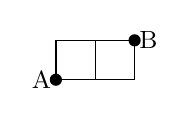
\begin{tikzpicture}[line width=0.5pt]
  \foreach \x in {0, 0.5, 1} { \draw (\x,0) -- (\x,0.5); }
  \foreach \y in {0, 0.5} { \draw (0,\y) -- (1,\y); }
  \fill (0,0) circle (2.2pt);
  \node[left, font=\small, inner sep=1.5pt] at (0,0) {$\pt{A}$};
  \fill (1,0.5) circle (2.2pt);
  \node[right, font=\small, inner sep=1.5pt] at (1,0.5) {$\pt{B}$};
\end{tikzpicture}
}\end{minipage}\par
\dmhint{$\pt{A}$에서 $\pt{B}$까지 최단 거리로 가려면 오른쪽으로 $\blank$칸, 위쪽으로 $\blank$칸 이동해야 한다.\\ 오른쪽으로 1칸 가는 것을 $a$, 위쪽으로 1칸 가는 것을 $b$라 하면 최단 거리로 가는 경우의 수는 $a$, $a$, $\blank$를 일렬로 나열하는 경우의 수와 같다.\\ 따라서 구하는 경우의 수는 $\dfrac{3!}{\blank!}=\blank$}
}\vspace{8mm}
\setcounter{dmproblemcount}{12}\dmpnum{14-13}{% id: 14-13
% book: 베이직쎈 확률과 통계 · 01 여러 가지 순열
% section: 개념 03 최단 거리로 가는 경우의 수
% passage: 다음 그림과 같은 도로망이 있다. $\pt{A}$에서 $\pt{B}$까지 최단 거리로 가는 경우의 수를 구하시오.
% figure: tikz:fig-14-13
% answer: 
% answer_source: 
% variant_level: 0 (원본 전사)
% 이 파일은 build.mjs 가 items.json 에서 만든다. 고칠 때는 items.json 을 고친다.
\smash{\raisebox{1.5mm}{\dmkichul{베이직쎈 확률과 통계 14쪽 13번}}}
\noindent\begin{minipage}[t]{0.58\linewidth}\vspace{0pt}\raggedright \end{minipage}\hfill\begin{minipage}[t]{0.4\linewidth}\vspace{0pt}\centering \resizebox{\ifdim\width>\linewidth\linewidth\else\width\fi}{!}{% 14-13(본책 14쪽) — 가로 3칸·세로 1칸 도로망(A 왼쪽 아래 · B 오른쪽 위). 스캔 그림을 TikZ 로 다시 그림(스캔 화질).
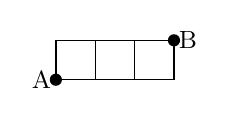
\begin{tikzpicture}[line width=0.5pt]
  \foreach \x in {0, 0.5, 1, 1.5} { \draw (\x,0) -- (\x,0.5); }
  \foreach \y in {0, 0.5} { \draw (0,\y) -- (1.5,\y); }
  \fill (0,0) circle (2.2pt);
  \node[left, font=\small, inner sep=1.5pt] at (0,0) {$\pt{A}$};
  \fill (1.5,0.5) circle (2.2pt);
  \node[right, font=\small, inner sep=1.5pt] at (1.5,0.5) {$\pt{B}$};
\end{tikzpicture}
}\end{minipage}\par
}\vspace{8mm}
\setcounter{dmproblemcount}{13}\dmpnum{14-14}{% id: 14-14
% book: 베이직쎈 확률과 통계 · 01 여러 가지 순열
% section: 개념 03 최단 거리로 가는 경우의 수
% passage: 다음 그림과 같은 도로망이 있다. $\pt{A}$에서 $\pt{B}$까지 최단 거리로 가는 경우의 수를 구하시오.
% figure: tikz:fig-14-14
% answer: 
% answer_source: 
% variant_level: 0 (원본 전사)
% 이 파일은 build.mjs 가 items.json 에서 만든다. 고칠 때는 items.json 을 고친다.
\smash{\raisebox{1.5mm}{\dmkichul{베이직쎈 확률과 통계 14쪽 14번}}}
\noindent\begin{minipage}[t]{0.58\linewidth}\vspace{0pt}\raggedright \end{minipage}\hfill\begin{minipage}[t]{0.4\linewidth}\vspace{0pt}\centering \resizebox{\ifdim\width>\linewidth\linewidth\else\width\fi}{!}{% 14-14(본책 14쪽) — 가로 2칸·세로 2칸 도로망(A 왼쪽 아래 · B 오른쪽 위). 스캔 그림을 TikZ 로 다시 그림(스캔 화질).
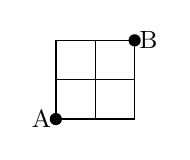
\begin{tikzpicture}[line width=0.5pt]
  \foreach \x in {0, 0.5, 1} { \draw (\x,0) -- (\x,1); }
  \foreach \y in {0, 0.5, 1} { \draw (0,\y) -- (1,\y); }
  \fill (0,0) circle (2.2pt);
  \node[left, font=\small, inner sep=1.5pt] at (0,0) {$\pt{A}$};
  \fill (1,1) circle (2.2pt);
  \node[right, font=\small, inner sep=1.5pt] at (1,1) {$\pt{B}$};
\end{tikzpicture}
}\end{minipage}\par
}\vspace{8mm}
\setcounter{dmproblemcount}{14}\dmpnum{14-15}{% id: 14-15
% book: 베이직쎈 확률과 통계 · 01 여러 가지 순열
% section: 개념 03 최단 거리로 가는 경우의 수
% passage: 다음 그림과 같은 도로망이 있다. $\pt{A}$에서 $\pt{B}$까지 최단 거리로 가는 경우의 수를 구하시오.
% figure: tikz:fig-14-15
% answer: 
% answer_source: 
% variant_level: 0 (원본 전사)
% 이 파일은 build.mjs 가 items.json 에서 만든다. 고칠 때는 items.json 을 고친다.
\smash{\raisebox{1.5mm}{\dmkichul{베이직쎈 확률과 통계 14쪽 15번}}}
\noindent\begin{minipage}[t]{0.58\linewidth}\vspace{0pt}\raggedright \end{minipage}\hfill\begin{minipage}[t]{0.4\linewidth}\vspace{0pt}\centering \resizebox{\ifdim\width>\linewidth\linewidth\else\width\fi}{!}{% 14-15(본책 14쪽) — 가로 3칸·세로 2칸 도로망(A 왼쪽 아래 · B 오른쪽 위). 스캔 그림을 TikZ 로 다시 그림(스캔 화질).
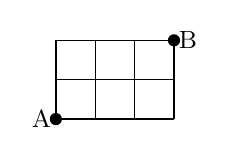
\begin{tikzpicture}[line width=0.5pt]
  \foreach \x in {0, 0.5, 1, 1.5} { \draw (\x,0) -- (\x,1); }
  \foreach \y in {0, 0.5, 1} { \draw (0,\y) -- (1.5,\y); }
  \fill (0,0) circle (2.2pt);
  \node[left, font=\small, inner sep=1.5pt] at (0,0) {$\pt{A}$};
  \fill (1.5,1) circle (2.2pt);
  \node[right, font=\small, inner sep=1.5pt] at (1.5,1) {$\pt{B}$};
\end{tikzpicture}
}\end{minipage}\par
}\vspace{8mm}
\dmpassage{다음 그림과 같은 도로망이 있다. $\pt{A}$에서 $\pt{P}$를 거쳐 $\pt{B}$까지 최단 거리로 가는 경우의 수를 구하시오.}
\setcounter{dmproblemcount}{15}\dmpnum{14-16}{% id: 14-16
% book: 베이직쎈 확률과 통계 · 01 여러 가지 순열
% section: 개념 03 최단 거리로 가는 경우의 수
% passage: 다음 그림과 같은 도로망이 있다. $\pt{A}$에서 $\pt{P}$를 거쳐 $\pt{B}$까지 최단 거리로 가는 경우의 수를 구하시오.
% figure: tikz:fig-14-16
% answer: 
% answer_source: 
% variant_level: 0 (원본 전사)
% 이 파일은 build.mjs 가 items.json 에서 만든다. 고칠 때는 items.json 을 고친다.
\smash{\raisebox{1.5mm}{\dmkichul{베이직쎈 확률과 통계 14쪽 16번}}}
\noindent\begin{minipage}[t]{0.58\linewidth}\vspace{0pt}\raggedright \end{minipage}\hfill\begin{minipage}[t]{0.4\linewidth}\vspace{0pt}\centering \resizebox{\ifdim\width>\linewidth\linewidth\else\width\fi}{!}{% 14-16(본책 14쪽) — 가로 4칸·세로 3칸 도로망(A 왼쪽 아래 · B 오른쪽 위 · P 는 오른쪽 3칸·위 1칸 지점). 스캔 그림을 TikZ 로 다시 그림(스캔 화질).
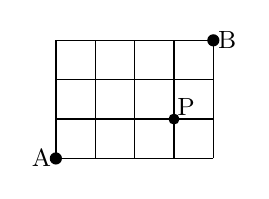
\begin{tikzpicture}[line width=0.5pt]
  \foreach \x in {0, 0.5, 1, 1.5, 2} { \draw (\x,0) -- (\x,1.5); }
  \foreach \y in {0, 0.5, 1, 1.5} { \draw (0,\y) -- (2,\y); }
  \fill (0,0) circle (2.2pt);
  \node[left, font=\small, inner sep=1.5pt] at (0,0) {$\pt{A}$};
  \fill (2,1.5) circle (2.2pt);
  \node[right, font=\small, inner sep=1.5pt] at (2,1.5) {$\pt{B}$};
  \fill (1.5,0.5) circle (2pt);
  \node[above right, font=\small, inner sep=1pt] at (1.5,0.5) {$\pt{P}$};
\end{tikzpicture}
}\end{minipage}\par
\dmhint{$\pt{A}$에서 $\pt{P}$까지 최단 거리로 가는 경우의 수는\\ $\dfrac{4!}{\blank!}=\blank$\\ $\pt{P}$에서 $\pt{B}$까지 최단 거리로 가는 경우의 수는\\ $\dfrac{3!}{\blank!}=3$\\ 따라서 구하는 경우의 수는 $\blank\cdot 3=\blank$}
}\vspace{8mm}
\setcounter{dmproblemcount}{16}\dmpnum{14-17}{% id: 14-17
% book: 베이직쎈 확률과 통계 · 01 여러 가지 순열
% section: 개념 03 최단 거리로 가는 경우의 수
% passage: 다음 그림과 같은 도로망이 있다. $\pt{A}$에서 $\pt{P}$를 거쳐 $\pt{B}$까지 최단 거리로 가는 경우의 수를 구하시오.
% figure: tikz:fig-14-17
% answer: 
% answer_source: 
% variant_level: 0 (원본 전사)
% 이 파일은 build.mjs 가 items.json 에서 만든다. 고칠 때는 items.json 을 고친다.
\smash{\raisebox{1.5mm}{\dmkichul{베이직쎈 확률과 통계 14쪽 17번}}}
\noindent\begin{minipage}[t]{0.58\linewidth}\vspace{0pt}\raggedright \end{minipage}\hfill\begin{minipage}[t]{0.4\linewidth}\vspace{0pt}\centering \resizebox{\ifdim\width>\linewidth\linewidth\else\width\fi}{!}{% 14-17(본책 14쪽) — 가로 4칸·세로 3칸 도로망(A 왼쪽 아래 · B 오른쪽 위 · P 는 오른쪽 2칸·위 1칸 지점). 스캔 그림을 TikZ 로 다시 그림(스캔 화질).
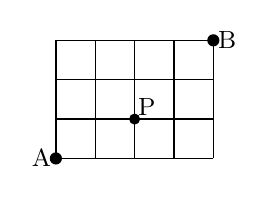
\begin{tikzpicture}[line width=0.5pt]
  \foreach \x in {0, 0.5, 1, 1.5, 2} { \draw (\x,0) -- (\x,1.5); }
  \foreach \y in {0, 0.5, 1, 1.5} { \draw (0,\y) -- (2,\y); }
  \fill (0,0) circle (2.2pt);
  \node[left, font=\small, inner sep=1.5pt] at (0,0) {$\pt{A}$};
  \fill (2,1.5) circle (2.2pt);
  \node[right, font=\small, inner sep=1.5pt] at (2,1.5) {$\pt{B}$};
  \fill (1,0.5) circle (2pt);
  \node[above right, font=\small, inner sep=1pt] at (1,0.5) {$\pt{P}$};
\end{tikzpicture}
}\end{minipage}\par
}\vspace{8mm}
\setcounter{dmproblemcount}{17}\dmpnum{14-18}{% id: 14-18
% book: 베이직쎈 확률과 통계 · 01 여러 가지 순열
% section: 개념 03 최단 거리로 가는 경우의 수
% passage: 다음 그림과 같은 도로망이 있다. $\pt{A}$에서 $\pt{P}$를 거쳐 $\pt{B}$까지 최단 거리로 가는 경우의 수를 구하시오.
% figure: tikz:fig-14-18
% answer: 
% answer_source: 
% variant_level: 0 (원본 전사)
% 이 파일은 build.mjs 가 items.json 에서 만든다. 고칠 때는 items.json 을 고친다.
\smash{\raisebox{1.5mm}{\dmkichul{베이직쎈 확률과 통계 14쪽 18번}}}
\noindent\begin{minipage}[t]{0.58\linewidth}\vspace{0pt}\raggedright \end{minipage}\hfill\begin{minipage}[t]{0.4\linewidth}\vspace{0pt}\centering \resizebox{\ifdim\width>\linewidth\linewidth\else\width\fi}{!}{% 14-18(본책 14쪽) — 가로 5칸·세로 3칸 도로망(A 왼쪽 아래 · B 오른쪽 위 · P 는 오른쪽 4칸·위 2칸 지점). 스캔 그림을 TikZ 로 다시 그림(스캔 화질).
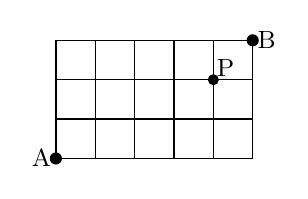
\begin{tikzpicture}[line width=0.5pt]
  \foreach \x in {0, 0.5, 1, 1.5, 2, 2.5} { \draw (\x,0) -- (\x,1.5); }
  \foreach \y in {0, 0.5, 1, 1.5} { \draw (0,\y) -- (2.5,\y); }
  \fill (0,0) circle (2.2pt);
  \node[left, font=\small, inner sep=1.5pt] at (0,0) {$\pt{A}$};
  \fill (2.5,1.5) circle (2.2pt);
  \node[right, font=\small, inner sep=1.5pt] at (2.5,1.5) {$\pt{B}$};
  \fill (2,1) circle (2pt);
  \node[above right, font=\small, inner sep=1pt] at (2,1) {$\pt{P}$};
\end{tikzpicture}
}\end{minipage}\par
}\vspace{8mm}
\dmsection{유형 006 같은 것이 있는 순열의 수; 문자를 나열하는 경우의 수}
\setcounter{dmproblemcount}{0}\dmpnum{15-01}{% id: 15-01
% book: 베이직쎈 확률과 통계 · 01 여러 가지 순열
% section: 유형 006 같은 것이 있는 순열의 수; 문자를 나열하는 경우의 수
% figure: none
% answer: 
% answer_source: 
% variant_level: 0 (원본 전사)
% 이 파일은 build.mjs 가 items.json 에서 만든다. 고칠 때는 items.json 을 고친다.
\smash{\raisebox{1.5mm}{\dmkichul{베이직쎈 확률과 통계 15쪽 01번}}}
interest에 있는 8개의 문자를 일렬로 나열할 때, 양 끝에 t가 오도록 나열하는 경우의 수는?
\dmchoicesauto{}{$360$}{$400$}{$440$}{$480$}{$520$}
}\vspace{8mm}
\setcounter{dmproblemcount}{1}\dmpnum{15-02}{% id: 15-02
% book: 베이직쎈 확률과 통계 · 01 여러 가지 순열
% section: 유형 006 같은 것이 있는 순열의 수; 문자를 나열하는 경우의 수
% figure: none
% answer: 
% answer_source: 
% variant_level: 0 (원본 전사)
% 이 파일은 build.mjs 가 items.json 에서 만든다. 고칠 때는 items.json 을 고친다.
\smash{\raisebox{1.5mm}{\dmkichul{베이직쎈 확률과 통계 15쪽 02번}}}
banana에 있는 6개의 문자를 일렬로 나열할 때, a끼리 이웃하게 나열하는 경우의 수는?
\dmchoicesauto{}{$6$}{$12$}{$18$}{$24$}{$30$}
}\vspace{8mm}
\setcounter{dmproblemcount}{2}\dmpnum{15-03}{% id: 15-03
% book: 베이직쎈 확률과 통계 · 01 여러 가지 순열
% section: 유형 006 같은 것이 있는 순열의 수; 문자를 나열하는 경우의 수
% figure: none
% answer: 
% answer_source: 
% variant_level: 0 (원본 전사)
% 이 파일은 build.mjs 가 items.json 에서 만든다. 고칠 때는 items.json 을 고친다.
\smash{\raisebox{1.5mm}{\dmkichul{베이직쎈 확률과 통계 15쪽 03번}}}
8개의 문자 $\mathrm{A}$, $\mathrm{A}$, $\mathrm{B}$, $\mathrm{B}$, $\mathrm{B}$, $\mathrm{B}$, $\mathrm{C}$, $\mathrm{D}$를 일렬로 나열할 때, $\mathrm{C}$와 $\mathrm{D}$가 이웃하지 않도록 나열하는 경우의 수를 구하시오.
}\vspace{8mm}
\dmsection{유형 007 같은 것이 있는 순열의 수; 자연수의 개수}
\setcounter{dmproblemcount}{3}\dmpnum{15-04}{% id: 15-04
% book: 베이직쎈 확률과 통계 · 01 여러 가지 순열
% section: 유형 007 같은 것이 있는 순열의 수; 자연수의 개수
% figure: none
% answer: 
% answer_source: 
% variant_level: 0 (원본 전사)
% 이 파일은 build.mjs 가 items.json 에서 만든다. 고칠 때는 items.json 을 고친다.
\smash{\raisebox{1.5mm}{\dmkichul{베이직쎈 확률과 통계 15쪽 04번}}}
5개의 숫자 $1$, $2$, $3$, $3$, $4$를 모두 이용하여 만들 수 있는 다섯 자리 자연수의 개수를 구하시오.
}\vspace{8mm}
\setcounter{dmproblemcount}{4}\dmpnum{15-05}{% id: 15-05
% book: 베이직쎈 확률과 통계 · 01 여러 가지 순열
% section: 유형 007 같은 것이 있는 순열의 수; 자연수의 개수
% figure: none
% answer: 
% answer_source: 
% variant_level: 0 (원본 전사)
% 이 파일은 build.mjs 가 items.json 에서 만든다. 고칠 때는 items.json 을 고친다.
\smash{\raisebox{1.5mm}{\dmkichul{베이직쎈 확률과 통계 15쪽 05번}}}
6개의 숫자 $0$, $1$, $1$, $2$, $2$, $2$를 모두 이용하여 만들 수 있는 여섯 자리 자연수의 개수는?
\dmchoicesauto{}{$35$}{$40$}{$45$}{$50$}{$55$}
}\vspace{8mm}
\setcounter{dmproblemcount}{5}\dmpnum{15-06}{% id: 15-06
% book: 베이직쎈 확률과 통계 · 01 여러 가지 순열
% section: 유형 007 같은 것이 있는 순열의 수; 자연수의 개수
% figure: none
% answer: 
% answer_source: 
% variant_level: 0 (원본 전사)
% 이 파일은 build.mjs 가 items.json 에서 만든다. 고칠 때는 items.json 을 고친다.
\smash{\raisebox{1.5mm}{\dmkichul{베이직쎈 확률과 통계 15쪽 06번}}}
6개의 숫자 $3$, $5$, $5$, $8$, $8$, $8$을 모두 이용하여 만들 수 있는 여섯 자리 자연수 중에서 홀수의 개수를 구하시오.
}\vspace{8mm}
\setcounter{dmproblemcount}{6}\dmpnum{15-07}{% id: 15-07
% book: 베이직쎈 확률과 통계 · 01 여러 가지 순열
% section: 유형 007 같은 것이 있는 순열의 수; 자연수의 개수
% figure: none
% answer: 
% answer_source: 
% variant_level: 0 (원본 전사)
% 이 파일은 build.mjs 가 items.json 에서 만든다. 고칠 때는 items.json 을 고친다.
\smash{\raisebox{1.5mm}{\dmkichul{베이직쎈 확률과 통계 15쪽 07번}}}
8개의 숫자 $2$, $2$, $3$, $4$, $5$, $6$, $6$, $6$을 모두 이용하여 만들 수 있는 여덟 자리 자연수 중에서 일의 자리, 십의 자리, 백의 자리, 천의 자리의 숫자가 모두 소수인 자연수의 개수는?
\dmchoicesauto{}{$32$}{$40$}{$48$}{$56$}{$64$}
}\vspace{8mm}
\setcounter{dmproblemcount}{7}\dmpnum{16-08}{% id: 16-08
% book: 베이직쎈 확률과 통계 · 01 여러 가지 순열
% section: 유형 007 같은 것이 있는 순열의 수; 자연수의 개수
% figure: none
% answer: 
% answer_source: 
% variant_level: 0 (원본 전사)
% 이 파일은 build.mjs 가 items.json 에서 만든다. 고칠 때는 items.json 을 고친다.
\smash{\raisebox{1.5mm}{\dmkichul{베이직쎈 확률과 통계 16쪽 08번}}}
5개의 숫자 $1$, $3$, $4$, $4$, $5$를 모두 이용하여 만들 수 있는 다섯 자리 자연수 중에서 $40000$보다 큰 자연수의 개수를 구하시오.
}\vspace{8mm}
\dmsection{유형 008 순서가 정해진 경우의 수}
\setcounter{dmproblemcount}{8}\dmpnum{16-09}{% id: 16-09
% book: 베이직쎈 확률과 통계 · 01 여러 가지 순열
% section: 유형 008 순서가 정해진 경우의 수
% figure: none
% answer: 
% answer_source: 
% variant_level: 0 (원본 전사)
% 이 파일은 build.mjs 가 items.json 에서 만든다. 고칠 때는 items.json 을 고친다.
\smash{\raisebox{1.5mm}{\dmkichul{베이직쎈 확률과 통계 16쪽 09번}}}
5개의 문자 $a$, $b$, $c$, $d$, $e$를 일렬로 나열할 때, $a$가 $d$보다 앞에 오도록 나열하는 경우의 수는?
\dmchoicesauto{}{$12$}{$24$}{$36$}{$48$}{$60$}
}\vspace{8mm}
\setcounter{dmproblemcount}{9}\dmpnum{16-10}{% id: 16-10
% book: 베이직쎈 확률과 통계 · 01 여러 가지 순열
% section: 유형 008 순서가 정해진 경우의 수
% figure: none
% answer: 
% answer_source: 
% variant_level: 0 (원본 전사)
% 이 파일은 build.mjs 가 items.json 에서 만든다. 고칠 때는 items.json 을 고친다.
\smash{\raisebox{1.5mm}{\dmkichul{베이직쎈 확률과 통계 16쪽 10번}}}
pleasure에 있는 8개의 문자를 일렬로 나열할 때, 모음을 알파벳 순서로 나열하는 경우의 수는?
\dmchoicesauto{}{$840$}{$1260$}{$1680$}{$2100$}{$2520$}
}\vspace{8mm}
\setcounter{dmproblemcount}{10}\dmpnum{16-11}{% id: 16-11
% book: 베이직쎈 확률과 통계 · 01 여러 가지 순열
% section: 유형 008 순서가 정해진 경우의 수
% figure: none
% answer: 
% answer_source: 
% variant_level: 0 (원본 전사)
% 이 파일은 build.mjs 가 items.json 에서 만든다. 고칠 때는 items.json 을 고친다.
\smash{\raisebox{1.5mm}{\dmkichul{베이직쎈 확률과 통계 16쪽 11번}}}
6개의 문자 $a$, $b$, $c$, $d$, $e$, $f$를 일렬로 나열할 때, 양 끝에 $a$, $b$가 오고 $c$는 $d$보다 앞에 오도록 나열하는 경우의 수를 구하시오.
}\vspace{8mm}
\setcounter{dmproblemcount}{11}\dmpnum{16-12}{% id: 16-12
% book: 베이직쎈 확률과 통계 · 01 여러 가지 순열
% section: 유형 008 순서가 정해진 경우의 수
% figure: none
% answer: 
% answer_source: 
% variant_level: 0 (원본 전사)
% 이 파일은 build.mjs 가 items.json 에서 만든다. 고칠 때는 items.json 을 고친다.
\smash{\raisebox{1.5mm}{\dmkichul{베이직쎈 확률과 통계 16쪽 12번}}}
7개의 숫자 $1$, $2$, $3$, $4$, $4$, $4$, $5$를 일렬로 나열할 때, $1$, $2$, $3$을 크기가 큰 것부터 순서대로 나열하는 경우의 수를 구하시오.
}\vspace{8mm}
\dmsection{유형 009 최단 거리로 가는 경우의 수}
\setcounter{dmproblemcount}{12}\dmpnum{16-13}{% id: 16-13
% book: 베이직쎈 확률과 통계 · 01 여러 가지 순열
% section: 유형 009 최단 거리로 가는 경우의 수
% figure: tikz:fig-16-13
% answer: 
% answer_source: 
% variant_level: 0 (원본 전사)
% 이 파일은 build.mjs 가 items.json 에서 만든다. 고칠 때는 items.json 을 고친다.
\smash{\raisebox{1.5mm}{\dmkichul{베이직쎈 확률과 통계 16쪽 13번}}}
\noindent\begin{minipage}[t]{0.58\linewidth}\vspace{0pt}\raggedright 오른쪽 그림과 같은 도로망이 있다. $\pt{A}$에서 $\pt{P}$를 거쳐 $\pt{B}$까지 최단 거리로 가는 경우의 수는?\end{minipage}\hfill\begin{minipage}[t]{0.4\linewidth}\vspace{0pt}\centering \resizebox{\ifdim\width>\linewidth\linewidth\else\width\fi}{!}{% 16-13(본책 16쪽) — 가로 5칸·세로 4칸 도로망(A 왼쪽 아래 · B 오른쪽 위 · P 는 오른쪽 2칸·위 1칸 지점). 스캔 그림을 TikZ 로 다시 그림(스캔 화질).
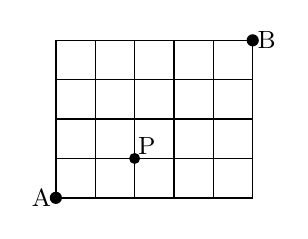
\begin{tikzpicture}[line width=0.5pt]
  \foreach \x in {0, 0.5, 1, 1.5, 2, 2.5} { \draw (\x,0) -- (\x,2); }
  \foreach \y in {0, 0.5, 1, 1.5, 2} { \draw (0,\y) -- (2.5,\y); }
  \fill (0,0) circle (2.2pt);
  \node[left, font=\small, inner sep=1.5pt] at (0,0) {$\pt{A}$};
  \fill (2.5,2) circle (2.2pt);
  \node[right, font=\small, inner sep=1.5pt] at (2.5,2) {$\pt{B}$};
  \fill (1,0.5) circle (2pt);
  \node[above right, font=\small, inner sep=1pt] at (1,0.5) {$\pt{P}$};
\end{tikzpicture}
}\end{minipage}\par
\dmchoicesauto{}{$48$}{$51$}{$54$}{$57$}{$60$}
}\vspace{8mm}
\setcounter{dmproblemcount}{13}\dmpnum{17-14}{% id: 17-14
% book: 베이직쎈 확률과 통계 · 01 여러 가지 순열
% section: 유형 009 최단 거리로 가는 경우의 수
% figure: tikz:fig-17-14
% answer: 
% answer_source: 
% variant_level: 0 (원본 전사)
% 이 파일은 build.mjs 가 items.json 에서 만든다. 고칠 때는 items.json 을 고친다.
\smash{\raisebox{1.5mm}{\dmkichul{베이직쎈 확률과 통계 17쪽 14번}}}
다음 그림과 같은 도로망이 있다. $\pt{A}$에서 $\pt{P}$, $\pt{Q}$를 모두 거쳐 $\pt{B}$까지 최단 거리로 가는 경우의 수는?
\par\smallskip\begin{center}\resizebox{\ifdim\width>\linewidth\linewidth\else\width\fi}{!}{% 17-14(본책 17쪽) — 가로 6칸·세로 4칸 도로망(A 왼쪽 위 · B 오른쪽 아래 · P, Q 는 위에서 1칸 내려온 가로줄의 오른쪽 3칸·4칸 지점). 스캔 그림을 TikZ 로 다시 그림(스캔 화질).
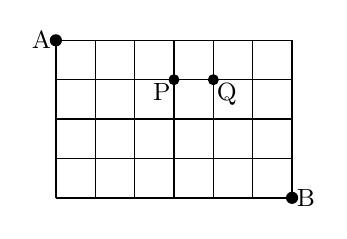
\begin{tikzpicture}[line width=0.5pt]
  \foreach \x in {0, 0.5, 1, 1.5, 2, 2.5, 3} { \draw (\x,0) -- (\x,2); }
  \foreach \y in {0, 0.5, 1, 1.5, 2} { \draw (0,\y) -- (3,\y); }
  \fill (0,2) circle (2.2pt);
  \node[left, font=\small, inner sep=1.5pt] at (0,2) {$\pt{A}$};
  \fill (3,0) circle (2.2pt);
  \node[right, font=\small, inner sep=1.5pt] at (3,0) {$\pt{B}$};
  \fill (1.5,1.5) circle (2pt);
  \node[below left, font=\small, inner sep=1pt] at (1.5,1.5) {$\pt{P}$};
  \fill (2,1.5) circle (2pt);
  \node[below right, font=\small, inner sep=1pt] at (2,1.5) {$\pt{Q}$};
\end{tikzpicture}
}\end{center}
\dmchoicesauto{}{$36$}{$38$}{$40$}{$42$}{$44$}
}\vspace{8mm}
\setcounter{dmproblemcount}{14}\dmpnum{17-15}{% id: 17-15
% book: 베이직쎈 확률과 통계 · 01 여러 가지 순열
% section: 유형 009 최단 거리로 가는 경우의 수
% figure: tikz:fig-17-15
% answer: 
% answer_source: 
% variant_level: 0 (원본 전사)
% 이 파일은 build.mjs 가 items.json 에서 만든다. 고칠 때는 items.json 을 고친다.
\smash{\raisebox{1.5mm}{\dmkichul{베이직쎈 확률과 통계 17쪽 15번}}}
\noindent\begin{minipage}[t]{0.58\linewidth}\vspace{0pt}\raggedright 오른쪽 그림과 같은 도로망이 있다. $\pt{A}$에서 $\pt{P}$를 거치지 않고 $\pt{B}$까지 최단 거리로 가는 경우의 수는?\end{minipage}\hfill\begin{minipage}[t]{0.4\linewidth}\vspace{0pt}\centering \resizebox{\ifdim\width>\linewidth\linewidth\else\width\fi}{!}{% 17-15(본책 17쪽) — 가로 5칸·세로 3칸 도로망(A 왼쪽 아래 · B 오른쪽 위 · P 는 오른쪽 2칸·위 1칸 지점). 스캔 그림을 TikZ 로 다시 그림(스캔 화질).
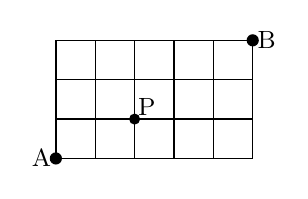
\begin{tikzpicture}[line width=0.5pt]
  \foreach \x in {0, 0.5, 1, 1.5, 2, 2.5} { \draw (\x,0) -- (\x,1.5); }
  \foreach \y in {0, 0.5, 1, 1.5} { \draw (0,\y) -- (2.5,\y); }
  \fill (0,0) circle (2.2pt);
  \node[left, font=\small, inner sep=1.5pt] at (0,0) {$\pt{A}$};
  \fill (2.5,1.5) circle (2.2pt);
  \node[right, font=\small, inner sep=1.5pt] at (2.5,1.5) {$\pt{B}$};
  \fill (1,0.5) circle (2pt);
  \node[above right, font=\small, inner sep=1pt] at (1,0.5) {$\pt{P}$};
\end{tikzpicture}
}\end{minipage}\par
\dmchoicesauto{}{$26$}{$27$}{$28$}{$29$}{$30$}
}\vspace{8mm}
\setcounter{dmproblemcount}{15}\dmpnum{17-16}{% id: 17-16
% book: 베이직쎈 확률과 통계 · 01 여러 가지 순열
% section: 유형 009 최단 거리로 가는 경우의 수
% figure: tikz:fig-17-16
% answer: 
% answer_source: 
% variant_level: 0 (원본 전사)
% 이 파일은 build.mjs 가 items.json 에서 만든다. 고칠 때는 items.json 을 고친다.
\smash{\raisebox{1.5mm}{\dmkichul{베이직쎈 확률과 통계 17쪽 16번}}}
\noindent\begin{minipage}[t]{0.58\linewidth}\vspace{0pt}\raggedright 오른쪽 그림과 같은 도로망이 있다. 다음을 구하시오.\end{minipage}\hfill\begin{minipage}[t]{0.4\linewidth}\vspace{0pt}\centering \resizebox{\ifdim\width>\linewidth\linewidth\else\width\fi}{!}{% 17-16(본책 17쪽) — 가로 6칸·세로 4칸 도로망(A 왼쪽 위 · B 오른쪽 아래 · P 는 오른쪽 2칸·아래 2칸 · Q 는 오른쪽 4칸·아래 3칸 지점). 스캔 그림을 TikZ 로 다시 그림(스캔 화질).
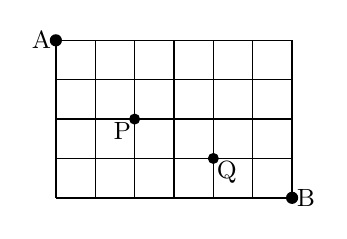
\begin{tikzpicture}[line width=0.5pt]
  \foreach \x in {0, 0.5, 1, 1.5, 2, 2.5, 3} { \draw (\x,0) -- (\x,2); }
  \foreach \y in {0, 0.5, 1, 1.5, 2} { \draw (0,\y) -- (3,\y); }
  \fill (0,2) circle (2.2pt);
  \node[left, font=\small, inner sep=1.5pt] at (0,2) {$\pt{A}$};
  \fill (3,0) circle (2.2pt);
  \node[right, font=\small, inner sep=1.5pt] at (3,0) {$\pt{B}$};
  \fill (1,1) circle (2pt);
  \node[below left, font=\small, inner sep=1pt] at (1,1) {$\pt{P}$};
  \fill (2,0.5) circle (2pt);
  \node[below right, font=\small, inner sep=1pt] at (2,0.5) {$\pt{Q}$};
\end{tikzpicture}
}\end{minipage}\par
\dmsubprob{1} $\pt{A}$에서 $\pt{P}$까지 최단 거리로 가는 경우의 수
\dmsubprob{2} $\pt{P}$에서 $\pt{Q}$를 거치지 않고 $\pt{B}$까지 최단 거리로 가는 경우의 수
\dmsubprob{3} $\pt{A}$에서 $\pt{B}$까지 최단 거리로 갈 때, $\pt{P}$는 거치고 $\pt{Q}$는 거치지 않고 가는 경우의 수
}\vspace{8mm}
\dmsection{유형 010 최단 거리로 가는 경우의 수; 중간 지점을 잡아야 하는 경우}
\setcounter{dmproblemcount}{16}\dmpnum{17-17}{% id: 17-17
% book: 베이직쎈 확률과 통계 · 01 여러 가지 순열
% section: 유형 010 최단 거리로 가는 경우의 수; 중간 지점을 잡아야 하는 경우
% figure: none
% answer: 
% answer_source: 
% variant_level: 0 (원본 전사)
% 이 파일은 build.mjs 가 items.json 에서 만든다. 고칠 때는 items.json 을 고친다.
\smash{\raisebox{1.5mm}{\dmkichul{베이직쎈 확률과 통계 17쪽 17번}}}
다음 그림과 같은 도로망이 있다. $\pt{A}$에서 $\pt{B}$까지 최단 거리로 가는 경우의 수를 구하시오.
\dmsubprob{1} % 17-17 ⑴(본책 17쪽) — 계단 모양 도로망(왼쪽 아래 2칸×1칸 블록 + 그 오른쪽 위로 2칸×2칸 블록 · 두 블록은 가운데 가로줄로 이어진다). A 왼쪽 아래 · B 오른쪽 위. 스캔 그림을 TikZ 로 다시 그림(스캔 화질).
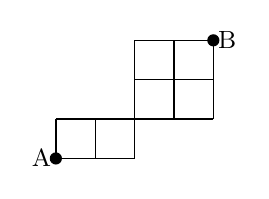
\begin{tikzpicture}[line width=0.5pt]
  % 아래 블록(가로 2칸·세로 1칸)
  \foreach \x in {0, 0.5, 1} { \draw (\x,0) -- (\x,0.5); }
  \draw (0,0) -- (1,0);
  % 두 블록을 잇는 가운데 가로줄
  \draw (0,0.5) -- (2,0.5);
  % 위 블록(가로 2칸·세로 2칸)
  \foreach \x in {1, 1.5, 2} { \draw (\x,0.5) -- (\x,1.5); }
  \foreach \y in {1, 1.5} { \draw (1,\y) -- (2,\y); }
  \fill (0,0) circle (2.2pt);
  \node[left, font=\small, inner sep=1.5pt] at (0,0) {$\pt{A}$};
  \fill (2,1.5) circle (2.2pt);
  \node[right, font=\small, inner sep=1.5pt] at (2,1.5) {$\pt{B}$};
\end{tikzpicture}

\dmsubprob{2} % 17-17 ⑵(본책 17쪽) — 가로 4칸·세로 3칸 도로망에서 가운데 가로줄 사이의 세로 도로 한 칸(왼쪽에서 둘째 세로줄·가운데 띠)이 없는 그림. A 왼쪽 위 · B 오른쪽 아래. 스캔 그림을 TikZ 로 다시 그림(스캔 화질).
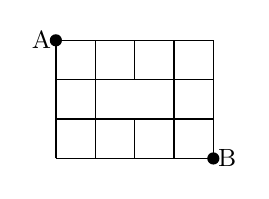
\begin{tikzpicture}[line width=0.5pt]
  \foreach \y in {0, 0.5, 1, 1.5} { \draw (0,\y) -- (2,\y); }
  \foreach \x in {0, 0.5, 1.5, 2} { \draw (\x,0) -- (\x,1.5); }
  \draw (1,0) -- (1,0.5);
  \draw (1,1) -- (1,1.5);
  \fill (0,1.5) circle (2.2pt);
  \node[left, font=\small, inner sep=1.5pt] at (0,1.5) {$\pt{A}$};
  \fill (2,0) circle (2.2pt);
  \node[right, font=\small, inner sep=1.5pt] at (2,0) {$\pt{B}$};
\end{tikzpicture}

}\vspace{8mm}
\setcounter{dmproblemcount}{17}\dmpnum{17-18}{% id: 17-18
% book: 베이직쎈 확률과 통계 · 01 여러 가지 순열
% section: 유형 010 최단 거리로 가는 경우의 수; 중간 지점을 잡아야 하는 경우
% figure: tikz:fig-17-18
% answer: 
% answer_source: 
% variant_level: 0 (원본 전사)
% 이 파일은 build.mjs 가 items.json 에서 만든다. 고칠 때는 items.json 을 고친다.
\smash{\raisebox{1.5mm}{\dmkichul{베이직쎈 확률과 통계 17쪽 18번}}}
\noindent\begin{minipage}[t]{0.58\linewidth}\vspace{0pt}\raggedright 오른쪽 그림과 같은 도로망이 있다. $\pt{A}$에서 $\pt{B}$까지 최단 거리로 가는 경우의 수를 구하시오.\end{minipage}\hfill\begin{minipage}[t]{0.4\linewidth}\vspace{0pt}\centering \resizebox{\ifdim\width>\linewidth\linewidth\else\width\fi}{!}{% 17-18(본책 17쪽) — ㄴ자 모양 도로망(아래 가로 4칸·세로 1칸 띠 + 그 오른쪽 위로 가로 2칸·세로 3칸 블록). A 왼쪽 아래 · B 오른쪽 위. 스캔 그림을 TikZ 로 다시 그림(스캔 화질).
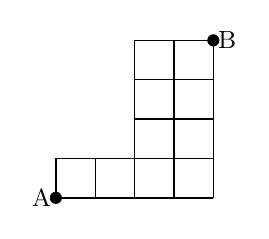
\begin{tikzpicture}[line width=0.5pt]
  % 아래 띠(가로 4칸·세로 1칸)
  \foreach \x in {0, 0.5, 1, 1.5, 2} { \draw (\x,0) -- (\x,0.5); }
  \foreach \y in {0, 0.5} { \draw (0,\y) -- (2,\y); }
  % 위 블록(가로 2칸·세로 3칸)
  \foreach \x in {1, 1.5, 2} { \draw (\x,0.5) -- (\x,2); }
  \foreach \y in {1, 1.5, 2} { \draw (1,\y) -- (2,\y); }
  \fill (0,0) circle (2.2pt);
  \node[left, font=\small, inner sep=1.5pt] at (0,0) {$\pt{A}$};
  \fill (2,2) circle (2.2pt);
  \node[right, font=\small, inner sep=1.5pt] at (2,2) {$\pt{B}$};
\end{tikzpicture}
}\end{minipage}\par
}\vspace{8mm}
\setcounter{dmproblemcount}{18}\dmpnum{17-19}{% id: 17-19
% book: 베이직쎈 확률과 통계 · 01 여러 가지 순열
% section: 유형 010 최단 거리로 가는 경우의 수; 중간 지점을 잡아야 하는 경우
% figure: tikz:fig-17-19
% answer: 
% answer_source: 
% variant_level: 0 (원본 전사)
% 이 파일은 build.mjs 가 items.json 에서 만든다. 고칠 때는 items.json 을 고친다.
\smash{\raisebox{1.5mm}{\dmkichul{베이직쎈 확률과 통계 17쪽 19번}}}
\noindent\begin{minipage}[t]{0.58\linewidth}\vspace{0pt}\raggedright 오른쪽 그림과 같은 도로망이 있다. $\pt{A}$에서 $\pt{B}$까지 최단 거리로 가는 경우의 수는?\end{minipage}\hfill\begin{minipage}[t]{0.4\linewidth}\vspace{0pt}\centering \resizebox{\ifdim\width>\linewidth\linewidth\else\width\fi}{!}{% 17-19(본책 17쪽) — 가로 4칸·세로 4칸 도로망 한가운데를 호수(하늘색 얼룩)가 덮어 가운데 교차점으로는 지날 수 없는 그림. A 왼쪽 위 · B 오른쪽 아래. 스캔 그림을 TikZ 로 다시 그림(스캔 화질 · 호수는 원문처럼 가운데 교차점과 그 둘레 네 도로만 덮는다 · 윤곽 모양은 스캔과 똑같지 않다).
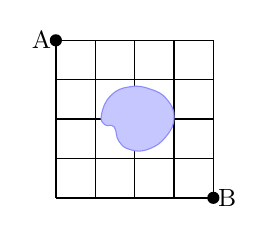
\begin{tikzpicture}[line width=0.5pt]
  \foreach \x in {0, 0.5, 1, 1.5, 2} { \draw (\x,0) -- (\x,2); }
  \foreach \y in {0, 0.5, 1, 1.5, 2} { \draw (0,\y) -- (2,\y); }
  \fill[blue!22, draw=blue!45, line width=0.4pt]
    plot[smooth cycle, tension=0.8] coordinates
    {(0.58,1.06) (0.70,1.30) (0.94,1.41) (1.20,1.38) (1.41,1.25) (1.50,1.02)
     (1.40,0.78) (1.18,0.62) (0.95,0.61) (0.80,0.72) (0.74,0.90) (0.62,0.93)};
  \fill (0,2) circle (2.2pt);
  \node[left, font=\small, inner sep=1.5pt] at (0,2) {$\pt{A}$};
  \fill (2,0) circle (2.2pt);
  \node[right, font=\small, inner sep=1.5pt] at (2,0) {$\pt{B}$};
\end{tikzpicture}
}\end{minipage}\par
\dmchoicesauto{}{$30$}{$31$}{$32$}{$33$}{$34$}
}\vspace{8mm}
\setcounter{dmproblemcount}{19}\dmpnum{17-20}{% id: 17-20
% book: 베이직쎈 확률과 통계 · 01 여러 가지 순열
% section: 유형 010 최단 거리로 가는 경우의 수; 중간 지점을 잡아야 하는 경우
% figure: tikz:fig-17-20
% answer: 
% answer_source: 
% variant_level: 0 (원본 전사)
% 이 파일은 build.mjs 가 items.json 에서 만든다. 고칠 때는 items.json 을 고친다.
\smash{\raisebox{1.5mm}{\dmkichul{베이직쎈 확률과 통계 17쪽 20번}}}
\noindent\begin{minipage}[t]{0.58\linewidth}\vspace{0pt}\raggedright 오른쪽 그림과 같은 도로망이 있다. $\pt{A}$에서 $\pt{B}$까지 최단 거리로 가는 경우의 수를 구하시오.\end{minipage}\hfill\begin{minipage}[t]{0.4\linewidth}\vspace{0pt}\centering \resizebox{\ifdim\width>\linewidth\linewidth\else\width\fi}{!}{% 17-20(본책 17쪽) — 가로 3칸·세로 5칸 도로망에서 가운데 왼쪽 두 칸 넓이만큼 도로가 없는 그림(왼쪽에서 둘째 세로줄은 위 1칸과 아래 2칸만, 위에서 셋째 가로줄은 오른쪽 1칸만 있다). A 왼쪽 위 · B 오른쪽 아래. 스캔 그림을 TikZ 로 다시 그림(스캔 화질).
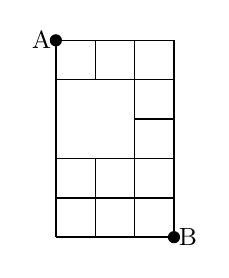
\begin{tikzpicture}[line width=0.5pt]
  % 가로줄 — 위에서 셋째(y=1.5)만 오른쪽 한 칸
  \foreach \y in {0, 0.5, 1, 2, 2.5} { \draw (0,\y) -- (1.5,\y); }
  \draw (1,1.5) -- (1.5,1.5);
  % 세로줄 — 왼쪽에서 둘째(x=0.5)는 위 1칸과 아래 2칸만
  \foreach \x in {0, 1, 1.5} { \draw (\x,0) -- (\x,2.5); }
  \draw (0.5,2) -- (0.5,2.5);
  \draw (0.5,0) -- (0.5,1);
  \fill (0,2.5) circle (2.2pt);
  \node[left, font=\small, inner sep=1.5pt] at (0,2.5) {$\pt{A}$};
  \fill (1.5,0) circle (2.2pt);
  \node[right, font=\small, inner sep=1.5pt] at (1.5,0) {$\pt{B}$};
\end{tikzpicture}
}\end{minipage}\par
}\vspace{8mm}
\dmsection{실전 감각 UP}
\setcounter{dmproblemcount}{0}\dmpnum{18-01}{% id: 18-01
% book: 베이직쎈 확률과 통계 · 01 여러 가지 순열
% section: 실전 감각 UP
% figure: none
% answer: 
% answer_source: 
% variant_level: 0 (원본 전사)
% 이 파일은 build.mjs 가 items.json 에서 만든다. 고칠 때는 items.json 을 고친다.
\smash{\raisebox{1.5mm}{\dmkichul{베이직쎈 확률과 통계 18쪽 01번}}}
5명의 등산가가 서로 다른 3개의 산 중에서 등산할 1개의 산을 각각 택하는 경우의 수는?
\dmchoicesauto{}{$81$}{$125$}{$162$}{$243$}{$256$}
}\vspace{8mm}
\setcounter{dmproblemcount}{1}\dmpnum{18-02}{% id: 18-02
% book: 베이직쎈 확률과 통계 · 01 여러 가지 순열
% section: 실전 감각 UP
% figure: none
% answer: 
% answer_source: 
% variant_level: 0 (원본 전사)
% 이 파일은 build.mjs 가 items.json 에서 만든다. 고칠 때는 items.json 을 고친다.
\smash{\raisebox{1.5mm}{\dmkichul{베이직쎈 확률과 통계 18쪽 02번 · 꼭 나와요}}}
6개의 특수 문자 @, \#, \$, \%, \&, $*$에서 중복을 허용하여 택한 3개를 일렬로 나열하여 만들 수 있는 암호의 개수는?
\dmchoicesauto{}{$108$}{$216$}{$432$}{$648$}{$729$}
}\vspace{8mm}
\setcounter{dmproblemcount}{2}\dmpnum{18-03}{% id: 18-03
% book: 베이직쎈 확률과 통계 · 01 여러 가지 순열
% section: 실전 감각 UP
% figure: none
% answer: 
% answer_source: 
% variant_level: 0 (원본 전사)
% 이 파일은 build.mjs 가 items.json 에서 만든다. 고칠 때는 items.json 을 고친다.
\smash{\raisebox{1.5mm}{\dmkichul{베이직쎈 확률과 통계 18쪽 03번}}}
6개의 숫자 $1$, $2$, $3$, $4$, $5$, $6$에서 중복을 허용하여 4개를 뽑아 만들 수 있는 네 자리 자연수 중에서 백의 자리의 숫자와 일의 자리의 숫자의 곱이 $6$인 자연수의 개수는?
\dmchoicesauto{}{$112$}{$128$}{$144$}{$160$}{$176$}
}\vspace{8mm}
\setcounter{dmproblemcount}{3}\dmpnum{18-04}{% id: 18-04
% book: 베이직쎈 확률과 통계 · 01 여러 가지 순열
% section: 실전 감각 UP
% figure: none
% answer: 
% answer_source: 
% variant_level: 0 (원본 전사)
% 이 파일은 build.mjs 가 items.json 에서 만든다. 고칠 때는 items.json 을 고친다.
\smash{\raisebox{1.5mm}{\dmkichul{베이직쎈 확률과 통계 18쪽 04번}}}
7개의 숫자 $1$, $2$, $3$, $4$, $5$, $6$, $7$에서 중복을 허용하여 4개를 뽑아 만들 수 있는 네 자리 자연수 중에서 $6000$ 이상인 짝수의 개수는?
\dmchoicesauto{}{$222$}{$240$}{$258$}{$276$}{$294$}
}\vspace{8mm}
\setcounter{dmproblemcount}{4}\dmpnum{18-05}{% id: 18-05
% book: 베이직쎈 확률과 통계 · 01 여러 가지 순열
% section: 실전 감각 UP
% figure: none
% answer: 
% answer_source: 
% variant_level: 0 (원본 전사)
% 이 파일은 build.mjs 가 items.json 에서 만든다. 고칠 때는 items.json 을 고친다.
\smash{\raisebox{1.5mm}{\dmkichul{베이직쎈 확률과 통계 18쪽 05번}}}
집합 $X=\{0{,}\mkern3mu\mathopen{}1{,}\mkern3mu\mathopen{}2{,}\mkern3mu\mathopen{}3{,}\mkern3mu\mathopen{}4\}$에 대하여 함수 $f:X\longrightarrow X$ 중에서 $f(1)+f(2)=2$를 만족시키는 함수의 개수는?
\dmchoicesauto{}{$50$}{$75$}{$150$}{$250$}{$375$}
}\vspace{8mm}
\setcounter{dmproblemcount}{5}\dmpnum{18-06}{% id: 18-06
% book: 베이직쎈 확률과 통계 · 01 여러 가지 순열
% section: 실전 감각 UP
% figure: none
% answer: 
% answer_source: 
% variant_level: 0 (원본 전사)
% 이 파일은 build.mjs 가 items.json 에서 만든다. 고칠 때는 items.json 을 고친다.
\smash{\raisebox{1.5mm}{\dmkichul{베이직쎈 확률과 통계 18쪽 06번 · 꼭 나와요}}}
7개의 자음 ㄱ, ㄱ, ㄴ, ㄴ, ㄴ, ㄷ, ㄹ을 일렬로 나열할 때, 양 끝에 ㄴ이 오도록 나열하는 경우의 수는?
\dmchoicesauto{}{$30$}{$60$}{$90$}{$120$}{$150$}
}\vspace{8mm}
\setcounter{dmproblemcount}{6}\dmpnum{18-07}{% id: 18-07
% book: 베이직쎈 확률과 통계 · 01 여러 가지 순열
% section: 실전 감각 UP
% figure: none
% answer: 
% answer_source: 
% variant_level: 0 (원본 전사)
% 이 파일은 build.mjs 가 items.json 에서 만든다. 고칠 때는 items.json 을 고친다.
\smash{\raisebox{1.5mm}{\dmkichul{베이직쎈 확률과 통계 18쪽 07번}}}
7개의 숫자 $0$, $3$, $3$, $3$, $3$, $4$, $4$가 각각 하나씩 적힌 7장의 카드를 모두 이용하여 만들 수 있는 일곱 자리 자연수 중에서 홀수의 개수는?
\dmchoicesauto{}{$50$}{$60$}{$70$}{$80$}{$90$}
}\vspace{8mm}
\setcounter{dmproblemcount}{7}\dmpnum{19-08}{% id: 19-08
% book: 베이직쎈 확률과 통계 · 01 여러 가지 순열
% section: 실전 감각 UP
% figure: tikz:fig-19-08
% answer: 
% answer_source: 
% variant_level: 0 (원본 전사)
% 이 파일은 build.mjs 가 items.json 에서 만든다. 고칠 때는 items.json 을 고친다.
\smash{\raisebox{1.5mm}{\dmkichul{베이직쎈 확률과 통계 19쪽 08번}}}
\noindent\begin{minipage}[t]{0.58\linewidth}\vspace{0pt}\raggedright 오른쪽 그림은 크기가 같은 정육면체 6개를 이어 붙여 만든 직육면체이다. 정육면체의 모서리를 따라 꼭짓점~$\pt{A}$에서 꼭짓점~$\pt{B}$까지 최단 거리로 가는 경우의 수는?\end{minipage}\hfill\begin{minipage}[t]{0.4\linewidth}\vspace{0pt}\centering \resizebox{\ifdim\width>\linewidth\linewidth\else\width\fi}{!}{% 19-08(19쪽) — 크기가 같은 정육면체 6개(가로 3 · 세로 2 · 높이 1)를 이어 붙인 직육면체와 꼭짓점 A, B.
% 스캔 화질이 낮아 TikZ 로 다시 그림(보이는 모서리 실선 · 숨은 모서리 파선 · 라벨은 원문에 있는 A, B 뿐 · 경우의 수는 적지 않는다).
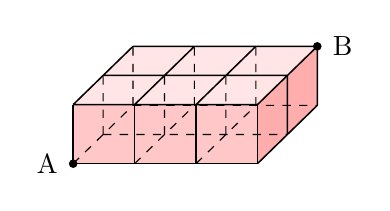
\begin{tikzpicture}[x={(0.78cm,0cm)},y={(0.38cm,0.37cm)},z={(0cm,0.75cm)},line width=0.55pt]
  \fill[red!10] (0,0,1) -- (3,0,1) -- (3,2,1) -- (0,2,1) -- cycle;
  \fill[red!22] (0,0,0) -- (3,0,0) -- (3,0,1) -- (0,0,1) -- cycle;
  \fill[red!32] (3,0,0) -- (3,2,0) -- (3,2,1) -- (3,0,1) -- cycle;
  % 숨은 모서리(아랫면 격자 · 왼쪽면 · 뒷면 · 속 모서리)
  \draw[dashed,line width=0.4pt] (0,0,0) -- (0,2,0) (1,0,0) -- (1,2,0) (2,0,0) -- (2,2,0)
    (0,1,0) -- (3,1,0) (0,2,0) -- (3,2,0)
    (0,1,0) -- (0,1,1) (0,2,0) -- (0,2,1) (1,1,0) -- (1,1,1) (1,2,0) -- (1,2,1)
    (2,1,0) -- (2,1,1) (2,2,0) -- (2,2,1);
  % 윗면 3x2 격자
  \draw (0,0,1) -- (3,0,1) (0,1,1) -- (3,1,1) (0,2,1) -- (3,2,1)
    (0,0,1) -- (0,2,1) (1,0,1) -- (1,2,1) (2,0,1) -- (2,2,1) (3,0,1) -- (3,2,1);
  % 앞면 3x1 · 오른쪽면 2x1
  \draw (0,0,0) -- (3,0,0) (0,0,0) -- (0,0,1) (1,0,0) -- (1,0,1) (2,0,0) -- (2,0,1) (3,0,0) -- (3,0,1);
  \draw (3,0,0) -- (3,2,0) (3,1,0) -- (3,1,1) (3,2,0) -- (3,2,1);
  \node[fill,circle,inner sep=1.1pt] at (0,0,0) {};
  \node[fill,circle,inner sep=1.1pt] at (3,2,1) {};
  \node[left=2pt] at (0,0,0) {$\pt{A}$};
  \node[right=2pt] at (3,2,1) {$\pt{B}$};
\end{tikzpicture}
}\end{minipage}\par
\dmchoicesauto{}{$52$}{$56$}{$60$}{$64$}{$68$}
}\vspace{8mm}
\setcounter{dmproblemcount}{8}\dmpnum{19-09}{% id: 19-09
% book: 베이직쎈 확률과 통계 · 01 여러 가지 순열
% section: 실전 감각 UP
% figure: none
% answer: 
% answer_source: 
% variant_level: 0 (원본 전사)
% 이 파일은 build.mjs 가 items.json 에서 만든다. 고칠 때는 items.json 을 고친다.
\smash{\raisebox{1.5mm}{\dmkichul{베이직쎈 확률과 통계 19쪽 09번 · 서답형}}}
서로 다른 7개의 쿠키를 세 주머니 $\mathrm{A}$, $\mathrm{B}$, $\mathrm{C}$에 남김없이 나누어 넣을 때, 주머니 $\mathrm{A}$에 넣은 쿠키의 개수가 $4$가 되도록 나누어 넣는 경우의 수를 구하시오. \dmcondfill{빈 주머니가 있을 수도 있다.}{}
}\vspace{8mm}
\setcounter{dmproblemcount}{9}\dmpnum{19-10}{% id: 19-10
% book: 베이직쎈 확률과 통계 · 01 여러 가지 순열
% section: 실전 감각 UP
% figure: none
% answer: 
% answer_source: 
% variant_level: 0 (원본 전사)
% 이 파일은 build.mjs 가 items.json 에서 만든다. 고칠 때는 items.json 을 고친다.
\smash{\raisebox{1.5mm}{\dmkichul{베이직쎈 확률과 통계 19쪽 10번 · 서답형 · 서술형}}}
노란색 깃발과 초록색 깃발이 각각 한 개씩 있다. 두 깃발을 합해서 $n$번 들어 올려서 128개의 신호를 만들 때, $n$의 값을 구하시오. \dmcondfill{두 깃발을 동시에 들어 올리지 않는다.}{}
}\vspace{8mm}
\setcounter{dmproblemcount}{10}\dmpnum{19-11}{% id: 19-11
% book: 베이직쎈 확률과 통계 · 01 여러 가지 순열
% section: 실전 감각 UP
% figure: none
% answer: 
% answer_source: 
% variant_level: 0 (원본 전사)
% 이 파일은 build.mjs 가 items.json 에서 만든다. 고칠 때는 items.json 을 고친다.
\smash{\raisebox{1.5mm}{\dmkichul{베이직쎈 확률과 통계 19쪽 11번 · 서술형}}}
4개의 숫자 $0$, $1$, $2$, $3$에서 중복을 허용하여 4개를 뽑아 네 자리 자연수를 만들 때, $2300$보다 작은 자연수의 개수를 구하시오.
}\vspace{8mm}
\setcounter{dmproblemcount}{11}\dmpnum{19-12}{% id: 19-12
% book: 베이직쎈 확률과 통계 · 01 여러 가지 순열
% section: 실전 감각 UP
% figure: none
% answer: 
% answer_source: 
% variant_level: 0 (원본 전사)
% 이 파일은 build.mjs 가 items.json 에서 만든다. 고칠 때는 items.json 을 고친다.
\smash{\raisebox{1.5mm}{\dmkichul{베이직쎈 확률과 통계 19쪽 12번 · 서답형 · 서술형}}}
9개의 숫자 $1$, $2$, $2$, $3$, $3$, $4$, $4$, $4$, $7$을 일렬로 나열할 때, 홀수를 짝수 번째 자리에 나열하는 경우의 수를 구하시오.
}\vspace{8mm}
\setcounter{dmproblemcount}{12}\dmpnum{19-13}{% id: 19-13
% book: 베이직쎈 확률과 통계 · 01 여러 가지 순열
% section: 실전 감각 UP
% figure: none
% answer: 
% answer_source: 
% variant_level: 0 (원본 전사)
% 이 파일은 build.mjs 가 items.json 에서 만든다. 고칠 때는 items.json 을 고친다.
\smash{\raisebox{1.5mm}{\dmkichul{베이직쎈 확률과 통계 19쪽 13번 · 서답형}}}
6개의 문자 $\mathrm{A}$, $\mathrm{B}$, $\mathrm{C}$, $\mathrm{D}$, $\mathrm{E}$, $\mathrm{F}$를 일렬로 나열할 때, $\mathrm{A}$는 $\mathrm{B}$보다 오른쪽에 나열하고 $\mathrm{C}$는 $\mathrm{D}$보다 왼쪽에 나열하는 경우의 수를 구하시오.
}\vspace{8mm}
\setcounter{dmproblemcount}{13}\dmpnum{19-14}{% id: 19-14
% book: 베이직쎈 확률과 통계 · 01 여러 가지 순열
% section: 실전 감각 UP
% figure: tikz:fig-19-14
% answer: 
% answer_source: 
% variant_level: 0 (원본 전사)
% 이 파일은 build.mjs 가 items.json 에서 만든다. 고칠 때는 items.json 을 고친다.
\smash{\raisebox{1.5mm}{\dmkichul{베이직쎈 확률과 통계 19쪽 14번}}}
다음 그림과 같이 도로망이 $\pt{P}$에서 서로 연결되어 있다. $\pt{A}$에서 $\pt{B}$까지 최단 거리로 가는 경우의 수를 구하시오.
\par\smallskip\begin{center}\resizebox{\ifdim\width>\linewidth\linewidth\else\width\fi}{!}{% 19-14(19쪽) — P 에서 서로 연결된 두 도로망(45도로 놓인 격자 · 왼쪽 2×3칸 · 오른쪽 2×2칸)과 지점 A, P, B.
% 스캔 화질이 낮아 TikZ 로 다시 그림(라벨은 원문에 있는 A, P, B 뿐 · 경우의 수는 그림에 적지 않는다).
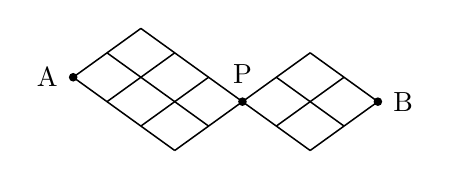
\begin{tikzpicture}[x={(0.43cm,0.31cm)},y={(0.43cm,-0.31cm)},line width=0.55pt]
  % 왼쪽 도로망: A(0,0) 에서 북동 2칸 · 남동 3칸
  \foreach \i in {0,1,2} \draw (\i,0) -- (\i,3);
  \foreach \j in {0,1,2,3} \draw (0,\j) -- (2,\j);
  % 오른쪽 도로망: P(2,3) 에서 북동 2칸 · 남동 2칸
  \foreach \i in {2,3,4} \draw (\i,3) -- (\i,5);
  \foreach \j in {3,4,5} \draw (2,\j) -- (4,\j);
  \node[fill,circle,inner sep=1.1pt] at (0,0) {};
  \node[fill,circle,inner sep=1.1pt] at (2,3) {};
  \node[fill,circle,inner sep=1.1pt] at (4,5) {};
  \node[left=2pt] at (0,0) {$\pt{A}$};
  \node[above=3pt] at (2,3) {$\pt{P}$};
  \node[right=2pt] at (4,5) {$\pt{B}$};
\end{tikzpicture}
}\end{center}
}\vspace{8mm}
\vspace*{0pt plus 1filll}
\clearpage
\renewcommand{\dmchapunit}{02 중복조합과 이항정리}
\dmchapter{02}{중복조합과 이항정리}
\setcounter{dmproblemcount}{0}
\dmsection{개념 04 중복조합}
\dmpassage{다음을 기호를 사용하여 ${}_n\mathrm{H}_r$ 꼴로 나타내시오.}
\setcounter{dmproblemcount}{0}\dmpnum{20-01}{% id: 20-01
% book: 베이직쎈 확률과 통계 · 02 중복조합과 이항정리
% section: 개념 04 중복조합
% passage: 다음을 기호를 사용하여 ${}_n\mathrm{H}_r$ 꼴로 나타내시오.
% figure: none
% answer: 
% answer_source: 
% variant_level: 0 (원본 전사)
% 이 파일은 build.mjs 가 items.json 에서 만든다. 고칠 때는 items.json 을 고친다.
\smash{\raisebox{1.5mm}{\dmkichul{베이직쎈 확률과 통계 20쪽 01번}}}
3개의 문자 $a$, $b$, $c$에서 2개를 택하는 중복조합의 수
}\vspace{8mm}
\setcounter{dmproblemcount}{1}\dmpnum{20-02}{% id: 20-02
% book: 베이직쎈 확률과 통계 · 02 중복조합과 이항정리
% section: 개념 04 중복조합
% passage: 다음을 기호를 사용하여 ${}_n\mathrm{H}_r$ 꼴로 나타내시오.
% figure: none
% answer: 
% answer_source: 
% variant_level: 0 (원본 전사)
% 이 파일은 build.mjs 가 items.json 에서 만든다. 고칠 때는 items.json 을 고친다.
\smash{\raisebox{1.5mm}{\dmkichul{베이직쎈 확률과 통계 20쪽 02번}}}
2개의 문자 $a$, $b$에서 5개를 택하는 중복조합의 수
}\vspace{8mm}
\setcounter{dmproblemcount}{2}\dmpnum{20-03}{% id: 20-03
% book: 베이직쎈 확률과 통계 · 02 중복조합과 이항정리
% section: 개념 04 중복조합
% passage: 다음을 기호를 사용하여 ${}_n\mathrm{H}_r$ 꼴로 나타내시오.
% figure: none
% answer: 
% answer_source: 
% variant_level: 0 (원본 전사)
% 이 파일은 build.mjs 가 items.json 에서 만든다. 고칠 때는 items.json 을 고친다.
\smash{\raisebox{1.5mm}{\dmkichul{베이직쎈 확률과 통계 20쪽 03번}}}
5개의 숫자 1, 2, 3, 4, 5에서 4개를 택하는 중복조합의 수
}\vspace{8mm}
\setcounter{dmproblemcount}{3}\dmpnum{20-04}{% id: 20-04
% book: 베이직쎈 확률과 통계 · 02 중복조합과 이항정리
% section: 개념 04 중복조합
% passage: 다음을 기호를 사용하여 ${}_n\mathrm{H}_r$ 꼴로 나타내시오.
% figure: none
% answer: 
% answer_source: 
% variant_level: 0 (원본 전사)
% 이 파일은 build.mjs 가 items.json 에서 만든다. 고칠 때는 items.json 을 고친다.
\smash{\raisebox{1.5mm}{\dmkichul{베이직쎈 확률과 통계 20쪽 04번}}}
4개의 숫자 0, 1, 2, 3에서 7개를 택하는 중복조합의 수
}\vspace{8mm}
\dmpassage{다음 값을 구하시오.}
\setcounter{dmproblemcount}{4}\dmpnum{20-05}{% id: 20-05
% book: 베이직쎈 확률과 통계 · 02 중복조합과 이항정리
% section: 개념 04 중복조합
% passage: 다음 값을 구하시오.
% figure: none
% answer: 
% answer_source: 
% variant_level: 0 (원본 전사)
% 이 파일은 build.mjs 가 items.json 에서 만든다. 고칠 때는 items.json 을 고친다.
\smash{\raisebox{1.5mm}{\dmkichul{베이직쎈 확률과 통계 20쪽 05번}}}
${}_4\mathrm{H}_2={}_{4+\text{\blank[1.2em]}-1}\mathrm{C}_{\text{\scriptsize\setlength{\fboxsep}{1.5pt}\framebox[1.5em]{\rule{0pt}{1.6ex}}}}=\blank$
}\vspace{8mm}
\setcounter{dmproblemcount}{5}\dmpnum{20-06}{% id: 20-06
% book: 베이직쎈 확률과 통계 · 02 중복조합과 이항정리
% section: 개념 04 중복조합
% passage: 다음 값을 구하시오.
% figure: none
% answer: 
% answer_source: 
% variant_level: 0 (원본 전사)
% 이 파일은 build.mjs 가 items.json 에서 만든다. 고칠 때는 items.json 을 고친다.
\smash{\raisebox{1.5mm}{\dmkichul{베이직쎈 확률과 통계 20쪽 06번}}}
${}_8\mathrm{H}_3$
}\vspace{8mm}
\setcounter{dmproblemcount}{6}\dmpnum{20-07}{% id: 20-07
% book: 베이직쎈 확률과 통계 · 02 중복조합과 이항정리
% section: 개념 04 중복조합
% passage: 다음 값을 구하시오.
% figure: none
% answer: 
% answer_source: 
% variant_level: 0 (원본 전사)
% 이 파일은 build.mjs 가 items.json 에서 만든다. 고칠 때는 items.json 을 고친다.
\smash{\raisebox{1.5mm}{\dmkichul{베이직쎈 확률과 통계 20쪽 07번}}}
${}_3\mathrm{H}_6$
}\vspace{8mm}
\setcounter{dmproblemcount}{7}\dmpnum{20-08}{% id: 20-08
% book: 베이직쎈 확률과 통계 · 02 중복조합과 이항정리
% section: 개념 04 중복조합
% passage: 다음 값을 구하시오.
% figure: none
% answer: 
% answer_source: 
% variant_level: 0 (원본 전사)
% 이 파일은 build.mjs 가 items.json 에서 만든다. 고칠 때는 items.json 을 고친다.
\smash{\raisebox{1.5mm}{\dmkichul{베이직쎈 확률과 통계 20쪽 08번}}}
${}_5\mathrm{H}_5$
}\vspace{8mm}
\dmpassage{다음을 만족시키는 자연수 $n$ 또는 $r$의 값을 구하시오.}
\setcounter{dmproblemcount}{8}\dmpnum{21-09}{% id: 21-09
% book: 베이직쎈 확률과 통계 · 02 중복조합과 이항정리
% section: 개념 04 중복조합
% passage: 다음을 만족시키는 자연수 $n$ 또는 $r$의 값을 구하시오.
% figure: none
% answer: 
% answer_source: 
% variant_level: 0 (원본 전사)
% 이 파일은 build.mjs 가 items.json 에서 만든다. 고칠 때는 items.json 을 고친다.
\smash{\raisebox{1.5mm}{\dmkichul{베이직쎈 확률과 통계 21쪽 09번}}}
${}_n\mathrm{H}_3={}_6\mathrm{C}_3$
}\vspace{8mm}
\setcounter{dmproblemcount}{9}\dmpnum{21-10}{% id: 21-10
% book: 베이직쎈 확률과 통계 · 02 중복조합과 이항정리
% section: 개념 04 중복조합
% passage: 다음을 만족시키는 자연수 $n$ 또는 $r$의 값을 구하시오.
% figure: none
% answer: 
% answer_source: 
% variant_level: 0 (원본 전사)
% 이 파일은 build.mjs 가 items.json 에서 만든다. 고칠 때는 items.json 을 고친다.
\smash{\raisebox{1.5mm}{\dmkichul{베이직쎈 확률과 통계 21쪽 10번}}}
${}_5\mathrm{H}_r={}_8\mathrm{C}_4$
}\vspace{8mm}
\setcounter{dmproblemcount}{10}\dmpnum{21-11}{% id: 21-11
% book: 베이직쎈 확률과 통계 · 02 중복조합과 이항정리
% section: 개념 04 중복조합
% passage: 다음을 만족시키는 자연수 $n$ 또는 $r$의 값을 구하시오.
% figure: none
% answer: 
% answer_source: 
% variant_level: 0 (원본 전사)
% 이 파일은 build.mjs 가 items.json 에서 만든다. 고칠 때는 items.json 을 고친다.
\smash{\raisebox{1.5mm}{\dmkichul{베이직쎈 확률과 통계 21쪽 11번}}}
${}_n\mathrm{H}_2=6$
\dmhint{${}_n\mathrm{H}_2={}_{\text{\scriptsize\setlength{\fboxsep}{1.5pt}\framebox[1.5em]{\rule{0pt}{1.6ex}}}}\mathrm{C}_2=\dfrac{(\blank[2.4em])n}{2\cdot 1}$이므로 ${}_n\mathrm{H}_2=6$에서\\ $\dfrac{(\blank[2.4em])n}{2\cdot 1}=6$, \quad $(\blank[2.4em])n=4\cdot\blank$\\ $\therefore\ n=\blank$}
}\vspace{8mm}
\setcounter{dmproblemcount}{11}\dmpnum{21-12}{% id: 21-12
% book: 베이직쎈 확률과 통계 · 02 중복조합과 이항정리
% section: 개념 04 중복조합
% passage: 다음을 만족시키는 자연수 $n$ 또는 $r$의 값을 구하시오.
% figure: none
% answer: 
% answer_source: 
% variant_level: 0 (원본 전사)
% 이 파일은 build.mjs 가 items.json 에서 만든다. 고칠 때는 items.json 을 고친다.
\smash{\raisebox{1.5mm}{\dmkichul{베이직쎈 확률과 통계 21쪽 12번}}}
${}_n\mathrm{H}_2=55$
}\vspace{8mm}
\setcounter{dmproblemcount}{12}\dmpnum{21-13}{% id: 21-13
% book: 베이직쎈 확률과 통계 · 02 중복조합과 이항정리
% section: 개념 04 중복조합
% passage: 다음을 만족시키는 자연수 $n$ 또는 $r$의 값을 구하시오.
% figure: none
% answer: 
% answer_source: 
% variant_level: 0 (원본 전사)
% 이 파일은 build.mjs 가 items.json 에서 만든다. 고칠 때는 items.json 을 고친다.
\smash{\raisebox{1.5mm}{\dmkichul{베이직쎈 확률과 통계 21쪽 13번}}}
${}_n\mathrm{H}_3=4$
}\vspace{8mm}
\dmpassage{다음을 구하시오.}
\setcounter{dmproblemcount}{13}\dmpnum{21-14}{% id: 21-14
% book: 베이직쎈 확률과 통계 · 02 중복조합과 이항정리
% section: 개념 04 중복조합
% passage: 다음을 구하시오.
% figure: none
% answer: 
% answer_source: 
% variant_level: 0 (원본 전사)
% 이 파일은 build.mjs 가 items.json 에서 만든다. 고칠 때는 items.json 을 고친다.
\smash{\raisebox{1.5mm}{\dmkichul{베이직쎈 확률과 통계 21쪽 14번}}}
서로 다른 2가지 색의 공 중에서 5개의 공을 택하는 경우의 수 \dmcondfill{같은 색의 공은 서로 구별하지 않는다.}{}
}\vspace{8mm}
\setcounter{dmproblemcount}{14}\dmpnum{21-15}{% id: 21-15
% book: 베이직쎈 확률과 통계 · 02 중복조합과 이항정리
% section: 개념 04 중복조합
% passage: 다음을 구하시오.
% figure: none
% answer: 
% answer_source: 
% variant_level: 0 (원본 전사)
% 이 파일은 build.mjs 가 items.json 에서 만든다. 고칠 때는 items.json 을 고친다.
\smash{\raisebox{1.5mm}{\dmkichul{베이직쎈 확률과 통계 21쪽 15번}}}
서로 다른 6가지 모양의 풍선 중에서 3개의 풍선을 고르는 경우의 수 \dmcondfill{같은 모양의 풍선은 서로 구별하지 않는다.}{}
}\vspace{8mm}
\setcounter{dmproblemcount}{15}\dmpnum{21-16}{% id: 21-16
% book: 베이직쎈 확률과 통계 · 02 중복조합과 이항정리
% section: 개념 04 중복조합
% passage: 다음을 구하시오.
% figure: none
% answer: 
% answer_source: 
% variant_level: 0 (원본 전사)
% 이 파일은 build.mjs 가 items.json 에서 만든다. 고칠 때는 items.json 을 고친다.
\smash{\raisebox{1.5mm}{\dmkichul{베이직쎈 확률과 통계 21쪽 16번}}}
사과, 딸기, 귤, 포도 중에서 8개의 과일을 고르는 경우의 수 \dmcondfill{같은 종류의 과일은 서로 구별하지 않는다.}{}
}\vspace{8mm}
\dmpassage{같은 종류의 음료수 5개를 3명의 학생에게 나누어 주려고 한다. 다음을 구하시오.}
\setcounter{dmproblemcount}{16}\dmpnum{21-17}{% id: 21-17
% book: 베이직쎈 확률과 통계 · 02 중복조합과 이항정리
% section: 개념 04 중복조합
% passage: 같은 종류의 음료수 5개를 3명의 학생에게 나누어 주려고 한다. 다음을 구하시오.
% figure: none
% answer: 
% answer_source: 
% variant_level: 0 (원본 전사)
% 이 파일은 build.mjs 가 items.json 에서 만든다. 고칠 때는 items.json 을 고친다.
\smash{\raisebox{1.5mm}{\dmkichul{베이직쎈 확률과 통계 21쪽 17번}}}
음료수를 학생들에게 나누어 주는 경우의 수 \dmcondfill{음료수를 받지 못하는 학생이 있을 수 있다.}{}
}\vspace{8mm}
\setcounter{dmproblemcount}{17}\dmpnum{21-18}{% id: 21-18
% book: 베이직쎈 확률과 통계 · 02 중복조합과 이항정리
% section: 개념 04 중복조합
% passage: 같은 종류의 음료수 5개를 3명의 학생에게 나누어 주려고 한다. 다음을 구하시오.
% figure: none
% answer: 
% answer_source: 
% variant_level: 0 (원본 전사)
% 이 파일은 build.mjs 가 items.json 에서 만든다. 고칠 때는 items.json 을 고친다.
\smash{\raisebox{1.5mm}{\dmkichul{베이직쎈 확률과 통계 21쪽 18번}}}
음료수를 학생들이 \underline{적어도 한 개씩 받도록} 나누어 주는 경우의 수
\dmhint{음료수를 학생들이 적어도 한 개씩 받으려면 먼저 음료수를 3명의 학생에게 각각 1개씩 나누어 주고, 나머지 \blank개의 음료수를 3명의 학생에게 나누어 주면 된다.\\ 따라서 구하는 경우의 수는 서로 다른 \blank개에서 \blank개를 택하는 중복조합의 수와 같으므로\\ ${}_{\text{\scriptsize\setlength{\fboxsep}{1.5pt}\framebox[1.5em]{\rule{0pt}{1.6ex}}}}\mathrm{H}_{\text{\scriptsize\setlength{\fboxsep}{1.5pt}\framebox[1.5em]{\rule{0pt}{1.6ex}}}}={}_{\text{\scriptsize\setlength{\fboxsep}{1.5pt}\framebox[1.5em]{\rule{0pt}{1.6ex}}}}\mathrm{C}_2=\blank$}
}\vspace{8mm}
\dmpassage{같은 종류의 펜 7자루를 서로 다른 4개의 필통에 넣으려고 한다. 다음을 구하시오.}
\setcounter{dmproblemcount}{18}\dmpnum{21-19}{% id: 21-19
% book: 베이직쎈 확률과 통계 · 02 중복조합과 이항정리
% section: 개념 04 중복조합
% passage: 같은 종류의 펜 7자루를 서로 다른 4개의 필통에 넣으려고 한다. 다음을 구하시오.
% figure: none
% answer: 
% answer_source: 
% variant_level: 0 (원본 전사)
% 이 파일은 build.mjs 가 items.json 에서 만든다. 고칠 때는 items.json 을 고친다.
\smash{\raisebox{1.5mm}{\dmkichul{베이직쎈 확률과 통계 21쪽 19번}}}
펜을 필통에 넣는 경우의 수 \dmcondfill{빈 필통이 있을 수 있다.}{}
}\vspace{8mm}
\setcounter{dmproblemcount}{19}\dmpnum{21-20}{% id: 21-20
% book: 베이직쎈 확률과 통계 · 02 중복조합과 이항정리
% section: 개념 04 중복조합
% passage: 같은 종류의 펜 7자루를 서로 다른 4개의 필통에 넣으려고 한다. 다음을 구하시오.
% figure: none
% answer: 
% answer_source: 
% variant_level: 0 (원본 전사)
% 이 파일은 build.mjs 가 items.json 에서 만든다. 고칠 때는 items.json 을 고친다.
\smash{\raisebox{1.5mm}{\dmkichul{베이직쎈 확률과 통계 21쪽 20번}}}
펜이 필통에 적어도 한 자루씩 들어가도록 넣는 경우의 수
}\vspace{8mm}
\dmsection{개념 05 순열, 중복순열, 조합, 중복조합의 비교}
\dmpassage{5개의 숫자 1, 2, 3, 4, 5에 대하여 다음을 구하시오.}
\setcounter{dmproblemcount}{20}\dmpnum{22-21}{% id: 22-21
% book: 베이직쎈 확률과 통계 · 02 중복조합과 이항정리
% section: 개념 05 순열, 중복순열, 조합, 중복조합의 비교
% passage: 5개의 숫자 1, 2, 3, 4, 5에 대하여 다음을 구하시오.
% figure: none
% answer: 
% answer_source: 
% variant_level: 0 (원본 전사)
% 이 파일은 build.mjs 가 items.json 에서 만든다. 고칠 때는 items.json 을 고친다.
\smash{\raisebox{1.5mm}{\dmkichul{베이직쎈 확률과 통계 22쪽 21번}}}
서로 다른 3개를 뽑아 만들 수 있는 세 자리 자연수의 개수
}\vspace{8mm}
\setcounter{dmproblemcount}{21}\dmpnum{22-22}{% id: 22-22
% book: 베이직쎈 확률과 통계 · 02 중복조합과 이항정리
% section: 개념 05 순열, 중복순열, 조합, 중복조합의 비교
% passage: 5개의 숫자 1, 2, 3, 4, 5에 대하여 다음을 구하시오.
% figure: none
% answer: 
% answer_source: 
% variant_level: 0 (원본 전사)
% 이 파일은 build.mjs 가 items.json 에서 만든다. 고칠 때는 items.json 을 고친다.
\smash{\raisebox{1.5mm}{\dmkichul{베이직쎈 확률과 통계 22쪽 22번}}}
중복을 허용하여 3개를 뽑아 만들 수 있는 세 자리 자연수의 개수
}\vspace{8mm}
\setcounter{dmproblemcount}{22}\dmpnum{22-23}{% id: 22-23
% book: 베이직쎈 확률과 통계 · 02 중복조합과 이항정리
% section: 개념 05 순열, 중복순열, 조합, 중복조합의 비교
% passage: 5개의 숫자 1, 2, 3, 4, 5에 대하여 다음을 구하시오.
% figure: none
% answer: 
% answer_source: 
% variant_level: 0 (원본 전사)
% 이 파일은 build.mjs 가 items.json 에서 만든다. 고칠 때는 items.json 을 고친다.
\smash{\raisebox{1.5mm}{\dmkichul{베이직쎈 확률과 통계 22쪽 23번}}}
서로 다른 3개를 택하는 경우의 수
}\vspace{8mm}
\setcounter{dmproblemcount}{23}\dmpnum{22-24}{% id: 22-24
% book: 베이직쎈 확률과 통계 · 02 중복조합과 이항정리
% section: 개념 05 순열, 중복순열, 조합, 중복조합의 비교
% passage: 5개의 숫자 1, 2, 3, 4, 5에 대하여 다음을 구하시오.
% figure: none
% answer: 
% answer_source: 
% variant_level: 0 (원본 전사)
% 이 파일은 build.mjs 가 items.json 에서 만든다. 고칠 때는 items.json 을 고친다.
\smash{\raisebox{1.5mm}{\dmkichul{베이직쎈 확률과 통계 22쪽 24번}}}
중복을 허용하여 3개를 택하는 경우의 수
}\vspace{8mm}
\dmpassage{두 집합 $X=\{1{,}\mkern3mu\mathopen{}2\}$, $Y=\{1{,}\mkern3mu\mathopen{}2{,}\mkern3mu\mathopen{}3\}$에 대하여 $a\in X$, $b\in X$일 때, 다음을 만족시키는 함수 $f:X\longrightarrow Y$의 개수를 구하시오.}
\setcounter{dmproblemcount}{24}\dmpnum{22-25}{% id: 22-25
% book: 베이직쎈 확률과 통계 · 02 중복조합과 이항정리
% section: 개념 05 순열, 중복순열, 조합, 중복조합의 비교
% passage: 두 집합 $X=\{1{,}\mkern3mu\mathopen{}2\}$, $Y=\{1{,}\mkern3mu\mathopen{}2{,}\mkern3mu\mathopen{}3\}$에 대하여 $a\in X$, $b\in X$일 때, 다음을 만족시키는 함수 $f:X\longrightarrow Y$의 개수를 구하시오.
% figure: none
% answer: 
% answer_source: 
% variant_level: 0 (원본 전사)
% 이 파일은 build.mjs 가 items.json 에서 만든다. 고칠 때는 items.json 을 고친다.
\smash{\raisebox{1.5mm}{\dmkichul{베이직쎈 확률과 통계 22쪽 25번}}}
$a<b$이면 $f(a)<f(b)$
\dmhint{$\Rightarrow$ $Y$의 원소 3개에서 서로 다른 \blank개를 뽑아 작은 수부터 차례대로 $X$의 원소 1, 2에 대응시키는 경우의 수\\ $\Rightarrow$ 서로 다른 3개에서 \blank개를 택하는 조합의 수\\ $\Rightarrow$ ${}_3\mathrm{C}_{\text{\scriptsize\setlength{\fboxsep}{1.5pt}\framebox[1.5em]{\rule{0pt}{1.6ex}}}}=\blank$}
}\vspace{8mm}
\setcounter{dmproblemcount}{25}\dmpnum{22-26}{% id: 22-26
% book: 베이직쎈 확률과 통계 · 02 중복조합과 이항정리
% section: 개념 05 순열, 중복순열, 조합, 중복조합의 비교
% passage: 두 집합 $X=\{1{,}\mkern3mu\mathopen{}2\}$, $Y=\{1{,}\mkern3mu\mathopen{}2{,}\mkern3mu\mathopen{}3\}$에 대하여 $a\in X$, $b\in X$일 때, 다음을 만족시키는 함수 $f:X\longrightarrow Y$의 개수를 구하시오.
% figure: none
% answer: 
% answer_source: 
% variant_level: 0 (원본 전사)
% 이 파일은 build.mjs 가 items.json 에서 만든다. 고칠 때는 items.json 을 고친다.
\smash{\raisebox{1.5mm}{\dmkichul{베이직쎈 확률과 통계 22쪽 26번}}}
$a<b$이면 $f(a)\le f(b)$
\dmhint{$\Rightarrow$ $Y$의 원소 3개에서 중복을 허용하여 \blank개를 뽑아 작거나 같은 수부터 차례대로 $X$의 원소 1, 2에 대응시키는 경우의 수\\ $\Rightarrow$ 서로 다른 3개에서 \blank개를 택하는 중복조합의 수\\ $\Rightarrow$ ${}_3\mathrm{H}_{\text{\scriptsize\setlength{\fboxsep}{1.5pt}\framebox[1.5em]{\rule{0pt}{1.6ex}}}}={}_{\text{\scriptsize\setlength{\fboxsep}{1.5pt}\framebox[1.5em]{\rule{0pt}{1.6ex}}}}\mathrm{C}_{\text{\scriptsize\setlength{\fboxsep}{1.5pt}\framebox[1.5em]{\rule{0pt}{1.6ex}}}}=\blank$}
}\vspace{8mm}
\dmpassage{두 집합 $X=\{5{,}\mkern3mu\mathopen{}6{,}\mkern3mu\mathopen{}7\}$, $Y=\{1{,}\mkern3mu\mathopen{}2{,}\mkern3mu\mathopen{}3{,}\mkern3mu\mathopen{}4\}$에 대하여 $a\in X$, $b\in X$일 때, 다음을 만족시키는 함수 $f:X\longrightarrow Y$의 개수를 구하시오.}
\setcounter{dmproblemcount}{26}\dmpnum{22-27}{% id: 22-27
% book: 베이직쎈 확률과 통계 · 02 중복조합과 이항정리
% section: 개념 05 순열, 중복순열, 조합, 중복조합의 비교
% passage: 두 집합 $X=\{5{,}\mkern3mu\mathopen{}6{,}\mkern3mu\mathopen{}7\}$, $Y=\{1{,}\mkern3mu\mathopen{}2{,}\mkern3mu\mathopen{}3{,}\mkern3mu\mathopen{}4\}$에 대하여 $a\in X$, $b\in X$일 때, 다음을 만족시키는 함수 $f:X\longrightarrow Y$의 개수를 구하시오.
% figure: none
% answer: 
% answer_source: 
% variant_level: 0 (원본 전사)
% 이 파일은 build.mjs 가 items.json 에서 만든다. 고칠 때는 items.json 을 고친다.
\smash{\raisebox{1.5mm}{\dmkichul{베이직쎈 확률과 통계 22쪽 27번}}}
$a<b$이면 $f(a)<f(b)$
}\vspace{8mm}
\setcounter{dmproblemcount}{27}\dmpnum{22-28}{% id: 22-28
% book: 베이직쎈 확률과 통계 · 02 중복조합과 이항정리
% section: 개념 05 순열, 중복순열, 조합, 중복조합의 비교
% passage: 두 집합 $X=\{5{,}\mkern3mu\mathopen{}6{,}\mkern3mu\mathopen{}7\}$, $Y=\{1{,}\mkern3mu\mathopen{}2{,}\mkern3mu\mathopen{}3{,}\mkern3mu\mathopen{}4\}$에 대하여 $a\in X$, $b\in X$일 때, 다음을 만족시키는 함수 $f:X\longrightarrow Y$의 개수를 구하시오.
% figure: none
% answer: 
% answer_source: 
% variant_level: 0 (원본 전사)
% 이 파일은 build.mjs 가 items.json 에서 만든다. 고칠 때는 items.json 을 고친다.
\smash{\raisebox{1.5mm}{\dmkichul{베이직쎈 확률과 통계 22쪽 28번}}}
$a<b$이면 $f(a)\le f(b)$
}\vspace{8mm}
\dmsection{개념 06 방정식의 해의 개수}
\dmpassage{다음 방정식의 음이 아닌 정수인 해의 개수를 구하시오.}
\setcounter{dmproblemcount}{28}\dmpnum{23-29}{% id: 23-29
% book: 베이직쎈 확률과 통계 · 02 중복조합과 이항정리
% section: 개념 06 방정식의 해의 개수
% passage: 다음 방정식의 음이 아닌 정수인 해의 개수를 구하시오.
% figure: none
% answer: 
% answer_source: 
% variant_level: 0 (원본 전사)
% 이 파일은 build.mjs 가 items.json 에서 만든다. 고칠 때는 items.json 을 고친다.
\smash{\raisebox{1.5mm}{\dmkichul{베이직쎈 확률과 통계 23쪽 29번}}}
$x+y+z=6$
\dmhint{구하는 해의 개수는 $x$, $y$, $z$의 3개에서 \blank개를 택하는 중복조합의 수와 같으므로\\ ${}_{\text{\scriptsize\setlength{\fboxsep}{1.5pt}\framebox[1.5em]{\rule{0pt}{1.6ex}}}}\mathrm{H}_{\text{\scriptsize\setlength{\fboxsep}{1.5pt}\framebox[1.5em]{\rule{0pt}{1.6ex}}}}={}_{\text{\scriptsize\setlength{\fboxsep}{1.5pt}\framebox[1.5em]{\rule{0pt}{1.6ex}}}}\mathrm{C}_6=\blank$}
}\vspace{8mm}
\setcounter{dmproblemcount}{29}\dmpnum{23-30}{% id: 23-30
% book: 베이직쎈 확률과 통계 · 02 중복조합과 이항정리
% section: 개념 06 방정식의 해의 개수
% passage: 다음 방정식의 음이 아닌 정수인 해의 개수를 구하시오.
% figure: none
% answer: 
% answer_source: 
% variant_level: 0 (원본 전사)
% 이 파일은 build.mjs 가 items.json 에서 만든다. 고칠 때는 items.json 을 고친다.
\smash{\raisebox{1.5mm}{\dmkichul{베이직쎈 확률과 통계 23쪽 30번}}}
$x+y+z=7$
}\vspace{8mm}
\setcounter{dmproblemcount}{30}\dmpnum{23-31}{% id: 23-31
% book: 베이직쎈 확률과 통계 · 02 중복조합과 이항정리
% section: 개념 06 방정식의 해의 개수
% passage: 다음 방정식의 음이 아닌 정수인 해의 개수를 구하시오.
% figure: none
% answer: 
% answer_source: 
% variant_level: 0 (원본 전사)
% 이 파일은 build.mjs 가 items.json 에서 만든다. 고칠 때는 items.json 을 고친다.
\smash{\raisebox{1.5mm}{\dmkichul{베이직쎈 확률과 통계 23쪽 31번}}}
$x+y+z=8$
}\vspace{8mm}
\setcounter{dmproblemcount}{31}\dmpnum{23-32}{% id: 23-32
% book: 베이직쎈 확률과 통계 · 02 중복조합과 이항정리
% section: 개념 06 방정식의 해의 개수
% passage: 다음 방정식의 음이 아닌 정수인 해의 개수를 구하시오.
% figure: none
% answer: 
% answer_source: 
% variant_level: 0 (원본 전사)
% 이 파일은 build.mjs 가 items.json 에서 만든다. 고칠 때는 items.json 을 고친다.
\smash{\raisebox{1.5mm}{\dmkichul{베이직쎈 확률과 통계 23쪽 32번}}}
$x+y+z+w=6$
}\vspace{8mm}
\dmpassage{다음 방정식의 양의 정수인 해의 개수를 구하시오.}
\setcounter{dmproblemcount}{32}\dmpnum{23-33}{% id: 23-33
% book: 베이직쎈 확률과 통계 · 02 중복조합과 이항정리
% section: 개념 06 방정식의 해의 개수
% passage: 다음 방정식의 양의 정수인 해의 개수를 구하시오.
% figure: none
% answer: 
% answer_source: 
% variant_level: 0 (원본 전사)
% 이 파일은 build.mjs 가 items.json 에서 만든다. 고칠 때는 items.json 을 고친다.
\smash{\raisebox{1.5mm}{\dmkichul{베이직쎈 확률과 통계 23쪽 33번}}}
$x+y+z=6$
\dmhint{$x$, $y$, $z$가 양의 정수이므로 $x-1=a$, $y-1=b$, $z-1=c$로 놓으면 $a$, $b$, $c$는 음이 아닌 정수이다. $x+y+z=6$에서\\ $a+b+c=\blank$ \cond{$a$, $b$, $c$는 음이 아닌 정수}\\ 따라서 구하는 해의 개수는 $a$, $b$, $c$의 3개에서 \blank개를 택하는 중복조합의 수와 같으므로\\ ${}_{\text{\scriptsize\setlength{\fboxsep}{1.5pt}\framebox[1.5em]{\rule{0pt}{1.6ex}}}}\mathrm{H}_{\text{\scriptsize\setlength{\fboxsep}{1.5pt}\framebox[1.5em]{\rule{0pt}{1.6ex}}}}={}_{\text{\scriptsize\setlength{\fboxsep}{1.5pt}\framebox[1.5em]{\rule{0pt}{1.6ex}}}}\mathrm{C}_3=\blank$}
}\vspace{8mm}
\setcounter{dmproblemcount}{33}\dmpnum{23-34}{% id: 23-34
% book: 베이직쎈 확률과 통계 · 02 중복조합과 이항정리
% section: 개념 06 방정식의 해의 개수
% passage: 다음 방정식의 양의 정수인 해의 개수를 구하시오.
% figure: none
% answer: 
% answer_source: 
% variant_level: 0 (원본 전사)
% 이 파일은 build.mjs 가 items.json 에서 만든다. 고칠 때는 items.json 을 고친다.
\smash{\raisebox{1.5mm}{\dmkichul{베이직쎈 확률과 통계 23쪽 34번}}}
$x+y+z=7$
}\vspace{8mm}
\setcounter{dmproblemcount}{34}\dmpnum{23-35}{% id: 23-35
% book: 베이직쎈 확률과 통계 · 02 중복조합과 이항정리
% section: 개념 06 방정식의 해의 개수
% passage: 다음 방정식의 양의 정수인 해의 개수를 구하시오.
% figure: none
% answer: 
% answer_source: 
% variant_level: 0 (원본 전사)
% 이 파일은 build.mjs 가 items.json 에서 만든다. 고칠 때는 items.json 을 고친다.
\smash{\raisebox{1.5mm}{\dmkichul{베이직쎈 확률과 통계 23쪽 35번}}}
$x+y+z=8$
}\vspace{8mm}
\setcounter{dmproblemcount}{35}\dmpnum{23-36}{% id: 23-36
% book: 베이직쎈 확률과 통계 · 02 중복조합과 이항정리
% section: 개념 06 방정식의 해의 개수
% passage: 다음 방정식의 양의 정수인 해의 개수를 구하시오.
% figure: none
% answer: 
% answer_source: 
% variant_level: 0 (원본 전사)
% 이 파일은 build.mjs 가 items.json 에서 만든다. 고칠 때는 items.json 을 고친다.
\smash{\raisebox{1.5mm}{\dmkichul{베이직쎈 확률과 통계 23쪽 36번}}}
$x+y+z+w=6$
}\vspace{8mm}
\dmsection{유형 011 중복조합의 수의 계산}
\setcounter{dmproblemcount}{0}\dmpnum{24-01}{% id: 24-01
% book: 베이직쎈 확률과 통계 · 02 중복조합과 이항정리
% section: 유형 011 중복조합의 수의 계산
% figure: none
% answer: 
% answer_source: 
% variant_level: 0 (원본 전사)
% 이 파일은 build.mjs 가 items.json 에서 만든다. 고칠 때는 items.json 을 고친다.
\smash{\raisebox{1.5mm}{\dmkichul{베이직쎈 확률과 통계 24쪽 01번}}}
${}_3\mathrm{P}_2+{}_2\mathrm{H}_5+{}_6\mathrm{C}_1$의 값은?
\dmchoicesauto{}{$12$}{$14$}{$16$}{$18$}{$20$}
}\vspace{8mm}
\setcounter{dmproblemcount}{1}\dmpnum{24-02}{% id: 24-02
% book: 베이직쎈 확률과 통계 · 02 중복조합과 이항정리
% section: 유형 011 중복조합의 수의 계산
% figure: none
% answer: 
% answer_source: 
% variant_level: 0 (원본 전사)
% 이 파일은 build.mjs 가 items.json 에서 만든다. 고칠 때는 items.json 을 고친다.
\smash{\raisebox{1.5mm}{\dmkichul{베이직쎈 확률과 통계 24쪽 02번}}}
${}_4\mathrm{H}_6={}_n\mathrm{C}_3$을 만족시키는 자연수 $n$에 대하여 ${}_{10}\mathrm{C}_n$의 값은?
\dmchoicesauto{}{$10$}{$45$}{$120$}{$210$}{$252$}
}\vspace{8mm}
\setcounter{dmproblemcount}{2}\dmpnum{24-03}{% id: 24-03
% book: 베이직쎈 확률과 통계 · 02 중복조합과 이항정리
% section: 유형 011 중복조합의 수의 계산
% figure: none
% answer: 
% answer_source: 
% variant_level: 0 (원본 전사)
% 이 파일은 build.mjs 가 items.json 에서 만든다. 고칠 때는 items.json 을 고친다.
\smash{\raisebox{1.5mm}{\dmkichul{베이직쎈 확률과 통계 24쪽 03번}}}
${}_3\mathrm{H}_r=28$을 만족시키는 자연수 $r$의 값을 구하시오.
}\vspace{8mm}
\setcounter{dmproblemcount}{3}\dmpnum{24-04}{% id: 24-04
% book: 베이직쎈 확률과 통계 · 02 중복조합과 이항정리
% section: 유형 011 중복조합의 수의 계산
% figure: none
% answer: 
% answer_source: 
% variant_level: 0 (원본 전사)
% 이 파일은 build.mjs 가 items.json 에서 만든다. 고칠 때는 items.json 을 고친다.
\smash{\raisebox{1.5mm}{\dmkichul{베이직쎈 확률과 통계 24쪽 04번}}}
${}_{9-r}\mathrm{H}_r={}_{11-r}\mathrm{H}_{r-2}$를 만족시키는 자연수 $r$의 값을 구하시오.
}\vspace{8mm}
\dmsection{유형 012 중복조합의 수}
\setcounter{dmproblemcount}{4}\dmpnum{24-05}{% id: 24-05
% book: 베이직쎈 확률과 통계 · 02 중복조합과 이항정리
% section: 유형 012 중복조합의 수
% figure: none
% answer: 
% answer_source: 
% variant_level: 0 (원본 전사)
% 이 파일은 build.mjs 가 items.json 에서 만든다. 고칠 때는 items.json 을 고친다.
\smash{\raisebox{1.5mm}{\dmkichul{베이직쎈 확률과 통계 24쪽 05번}}}
야채김밥, 치즈김밥, 참치김밥만을 판매하는 분식집에서 김밥 4줄을 구매하는 경우의 수는? \dmcondfill{같은 종류의 김밥은 서로 구별하지 않는다.}{}
\dmchoicesauto{}{$13$}{$14$}{$15$}{$16$}{$17$}
}\vspace{8mm}
\setcounter{dmproblemcount}{5}\dmpnum{24-06}{% id: 24-06
% book: 베이직쎈 확률과 통계 · 02 중복조합과 이항정리
% section: 유형 012 중복조합의 수
% figure: none
% answer: 
% answer_source: 
% variant_level: 0 (원본 전사)
% 이 파일은 build.mjs 가 items.json 에서 만든다. 고칠 때는 items.json 을 고친다.
\smash{\raisebox{1.5mm}{\dmkichul{베이직쎈 확률과 통계 24쪽 06번}}}
빨간 구슬 5개, 노란 구슬 8개, 흰 구슬 7개가 들어 있는 주머니에서 5개의 구슬을 꺼내는 경우의 수를 구하시오. \dmcondfill{같은 색의 구슬은 서로 구별하지 않는다.}{}
}\vspace{8mm}
\setcounter{dmproblemcount}{6}\dmpnum{24-07}{% id: 24-07
% book: 베이직쎈 확률과 통계 · 02 중복조합과 이항정리
% section: 유형 012 중복조합의 수
% figure: none
% answer: 
% answer_source: 
% variant_level: 0 (원본 전사)
% 이 파일은 build.mjs 가 items.json 에서 만든다. 고칠 때는 items.json 을 고친다.
\smash{\raisebox{1.5mm}{\dmkichul{베이직쎈 확률과 통계 24쪽 07번}}}
2명의 후보가 출마한 선거에서 6명의 유권자가 한 명의 후보에게 각각 투표하려고 한다. 무기명으로 투표할 때, 투표 결과의 경우의 수는? \dmcondfill{기권이나 무효표는 없다.}{}
\dmchoicesauto{}{$5$}{$7$}{$9$}{$11$}{$13$}
}\vspace{8mm}
\setcounter{dmproblemcount}{7}\dmpnum{25-08}{% id: 25-08
% book: 베이직쎈 확률과 통계 · 02 중복조합과 이항정리
% section: 유형 012 중복조합의 수
% figure: none
% answer: 
% answer_source: 
% variant_level: 0 (원본 전사)
% 이 파일은 build.mjs 가 items.json 에서 만든다. 고칠 때는 items.json 을 고친다.
\smash{\raisebox{1.5mm}{\dmkichul{베이직쎈 확률과 통계 25쪽 08번}}}
야구공 5개와 농구공 4개를 서로 다른 두 상자 $\mathrm{A}$, $\mathrm{B}$에 나누어 넣는 경우의 수는? \dmcondfill{같은 종류의 공은 서로 구별하지 않고, 빈 상자가 있을 수 있다.}{}
\dmchoicesauto{}{$14$}{$18$}{$22$}{$26$}{$30$}
}\vspace{8mm}
\dmsection{유형 013 중복조합의 수; ‘적어도’의 조건이 있는 경우}
\setcounter{dmproblemcount}{8}\dmpnum{25-09}{% id: 25-09
% book: 베이직쎈 확률과 통계 · 02 중복조합과 이항정리
% section: 유형 013 중복조합의 수; ‘적어도’의 조건이 있는 경우
% figure: none
% answer: 
% answer_source: 
% variant_level: 0 (원본 전사)
% 이 파일은 build.mjs 가 items.json 에서 만든다. 고칠 때는 items.json 을 고친다.
\smash{\raisebox{1.5mm}{\dmkichul{베이직쎈 확률과 통계 25쪽 09번}}}
같은 종류의 사탕 12개를 3명의 학생에게 나누어 주려고 한다. 이때 각 학생이 적어도 한 개씩 받도록 나누어 주는 경우의 수는?
\dmchoicesauto{}{$55$}{$58$}{$61$}{$64$}{$67$}
}\vspace{8mm}
\setcounter{dmproblemcount}{9}\dmpnum{25-10}{% id: 25-10
% book: 베이직쎈 확률과 통계 · 02 중복조합과 이항정리
% section: 유형 013 중복조합의 수; ‘적어도’의 조건이 있는 경우
% figure: none
% answer: 
% answer_source: 
% variant_level: 0 (원본 전사)
% 이 파일은 build.mjs 가 items.json 에서 만든다. 고칠 때는 items.json 을 고친다.
\smash{\raisebox{1.5mm}{\dmkichul{베이직쎈 확률과 통계 25쪽 10번}}}
같은 종류의 연필 8자루를 서로 다른 5개의 연필꽂이에 꽂으려고 한다. 빈 연필꽂이가 없도록 연필을 꽂는 경우의 수를 구하시오.
}\vspace{8mm}
\setcounter{dmproblemcount}{10}\dmpnum{25-11}{% id: 25-11
% book: 베이직쎈 확률과 통계 · 02 중복조합과 이항정리
% section: 유형 013 중복조합의 수; ‘적어도’의 조건이 있는 경우
% figure: none
% answer: 
% answer_source: 
% variant_level: 0 (원본 전사)
% 이 파일은 build.mjs 가 items.json 에서 만든다. 고칠 때는 items.json 을 고친다.
\smash{\raisebox{1.5mm}{\dmkichul{베이직쎈 확률과 통계 25쪽 11번}}}
흰 공, 파란 공, 검은 공이 각각 5개씩 들어 있는 상자에서 8개의 공을 꺼낼 때, 각 색깔의 공이 적어도 두 개씩은 포함되도록 꺼내는 경우의 수는? \dmcondfill{같은 색의 공은 서로 구별하지 않는다.}{}
\dmchoicesauto{}{$6$}{$7$}{$8$}{$9$}{$10$}
}\vspace{8mm}
\setcounter{dmproblemcount}{11}\dmpnum{25-12}{% id: 25-12
% book: 베이직쎈 확률과 통계 · 02 중복조합과 이항정리
% section: 유형 013 중복조합의 수; ‘적어도’의 조건이 있는 경우
% figure: none
% answer: 
% answer_source: 
% variant_level: 0 (원본 전사)
% 이 파일은 build.mjs 가 items.json 에서 만든다. 고칠 때는 items.json 을 고친다.
\smash{\raisebox{1.5mm}{\dmkichul{베이직쎈 확률과 통계 25쪽 12번}}}
딸기 맛 우유, 초콜릿 맛 우유 중에서 9개의 우유를 택할 때, 초콜릿 맛 우유를 2개 이상 택하는 경우의 수를 구하시오. \dmcondfill{같은 맛의 우유는 서로 구별하지 않고, 딸기 맛 우유를 하나도 택하지 않을 수 있다.}{}
}\vspace{8mm}
\dmsection{유형 014 전개식의 항의 개수}
\setcounter{dmproblemcount}{12}\dmpnum{25-13}{% id: 25-13
% book: 베이직쎈 확률과 통계 · 02 중복조합과 이항정리
% section: 유형 014 전개식의 항의 개수
% figure: none
% answer: 
% answer_source: 
% variant_level: 0 (원본 전사)
% 이 파일은 build.mjs 가 items.json 에서 만든다. 고칠 때는 items.json 을 고친다.
\smash{\raisebox{1.5mm}{\dmkichul{베이직쎈 확률과 통계 25쪽 13번}}}
다음 식의 전개식에서 서로 다른 항의 개수를 구하시오.
\dmsubprob{1} $(a+b+c)^8$
\dmsubprob{2} $(a+b+c+d)^6$
}\vspace{8mm}
\setcounter{dmproblemcount}{13}\dmpnum{26-14}{% id: 26-14
% book: 베이직쎈 확률과 통계 · 02 중복조합과 이항정리
% section: 유형 014 전개식의 항의 개수
% figure: none
% answer: 
% answer_source: 
% variant_level: 0 (원본 전사)
% 이 파일은 build.mjs 가 items.json 에서 만든다. 고칠 때는 items.json 을 고친다.
\smash{\raisebox{1.5mm}{\dmkichul{베이직쎈 확률과 통계 26쪽 14번}}}
$(a+b)^6(c+d+e)^3$의 전개식에 대하여 다음을 구하시오.
\dmsubprob{1} $(a+b)^6$의 전개식에서 서로 다른 항의 개수
\dmsubprob{2} $(c+d+e)^3$의 전개식에서 서로 다른 항의 개수
\dmsubprob{3} $(a+b)^6(c+d+e)^3$의 전개식에서 서로 다른 항의 개수
}\vspace{8mm}
\dmsection{유형 015 방정식의 해의 개수}
\setcounter{dmproblemcount}{14}\dmpnum{26-15}{% id: 26-15
% book: 베이직쎈 확률과 통계 · 02 중복조합과 이항정리
% section: 유형 015 방정식의 해의 개수
% figure: none
% answer: 
% answer_source: 
% variant_level: 0 (원본 전사)
% 이 파일은 build.mjs 가 items.json 에서 만든다. 고칠 때는 items.json 을 고친다.
\smash{\raisebox{1.5mm}{\dmkichul{베이직쎈 확률과 통계 26쪽 15번}}}
방정식 $x+y+z=9$를 만족시키는 음이 아닌 정수 $x$, $y$, $z$의 순서쌍 $(x{,}\mkern3mu\mathopen{}y{,}\mkern3mu\mathopen{}z)$의 개수는?
\dmchoicesauto{}{$46$}{$49$}{$52$}{$55$}{$58$}
}\vspace{8mm}
\setcounter{dmproblemcount}{15}\dmpnum{26-16}{% id: 26-16
% book: 베이직쎈 확률과 통계 · 02 중복조합과 이항정리
% section: 유형 015 방정식의 해의 개수
% figure: none
% answer: 
% answer_source: 
% variant_level: 0 (원본 전사)
% 이 파일은 build.mjs 가 items.json 에서 만든다. 고칠 때는 items.json 을 고친다.
\smash{\raisebox{1.5mm}{\dmkichul{베이직쎈 확률과 통계 26쪽 16번}}}
다음 각 경우에 대하여 방정식 $x+y+z+w=10$을 만족시키는 $x$, $y$, $z$, $w$의 순서쌍 $(x{,}\mkern3mu\mathopen{}y{,}\mkern3mu\mathopen{}z{,}\mkern3mu\mathopen{}w)$의 개수를 구하시오.
\dmsubprob{1} $x$, $y$, $z$, $w$가 음이 아닌 정수인 경우
\dmsubprob{2} $x$, $y$, $z$, $w$가 양의 정수인 경우
}\vspace{8mm}
\setcounter{dmproblemcount}{16}\dmpnum{26-17}{% id: 26-17
% book: 베이직쎈 확률과 통계 · 02 중복조합과 이항정리
% section: 유형 015 방정식의 해의 개수
% figure: none
% answer: 
% answer_source: 
% variant_level: 0 (원본 전사)
% 이 파일은 build.mjs 가 items.json 에서 만든다. 고칠 때는 items.json 을 고친다.
\smash{\raisebox{1.5mm}{\dmkichul{베이직쎈 확률과 통계 26쪽 17번}}}
방정식 $x+y+z=11$을 만족시키는 $x\ge 1$, $y\ge 2$, $z\ge 3$인 정수 $x$, $y$, $z$의 순서쌍 $(x{,}\mkern3mu\mathopen{}y{,}\mkern3mu\mathopen{}z)$의 개수는?
\dmchoicesauto{}{$17$}{$18$}{$19$}{$20$}{$21$}
}\vspace{8mm}
\setcounter{dmproblemcount}{17}\dmpnum{26-18}{% id: 26-18
% book: 베이직쎈 확률과 통계 · 02 중복조합과 이항정리
% section: 유형 015 방정식의 해의 개수
% figure: none
% answer: 
% answer_source: 
% variant_level: 0 (원본 전사)
% 이 파일은 build.mjs 가 items.json 에서 만든다. 고칠 때는 items.json 을 고친다.
\smash{\raisebox{1.5mm}{\dmkichul{베이직쎈 확률과 통계 26쪽 18번}}}
부등식 $x+y+z\le 2$를 만족시키는 음이 아닌 정수 $x$, $y$, $z$에 대하여 다음을 구하시오.
\dmsubprob{1} $x+y+z$가 가질 수 있는 값
\dmsubprob{2} 순서쌍 $(x{,}\mkern3mu\mathopen{}y{,}\mkern3mu\mathopen{}z)$의 개수
}\vspace{8mm}
\dmsection{유형 016 대소 관계가 정해진 순서쌍의 개수}
\setcounter{dmproblemcount}{18}\dmpnum{26-19}{% id: 26-19
% book: 베이직쎈 확률과 통계 · 02 중복조합과 이항정리
% section: 유형 016 대소 관계가 정해진 순서쌍의 개수
% figure: none
% answer: 
% answer_source: 
% variant_level: 0 (원본 전사)
% 이 파일은 build.mjs 가 items.json 에서 만든다. 고칠 때는 items.json 을 고친다.
\smash{\raisebox{1.5mm}{\dmkichul{베이직쎈 확률과 통계 26쪽 19번}}}
$a\le b\le 8$을 만족시키는 자연수 $a$, $b$의 순서쌍 $(a{,}\mkern3mu\mathopen{}b)$의 개수는?
\dmchoicesauto{}{$32$}{$33$}{$34$}{$35$}{$36$}
}\vspace{8mm}
\setcounter{dmproblemcount}{19}\dmpnum{27-20}{% id: 27-20
% book: 베이직쎈 확률과 통계 · 02 중복조합과 이항정리
% section: 유형 016 대소 관계가 정해진 순서쌍의 개수
% figure: none
% answer: 
% answer_source: 
% variant_level: 0 (원본 전사)
% 이 파일은 build.mjs 가 items.json 에서 만든다. 고칠 때는 items.json 을 고친다.
\smash{\raisebox{1.5mm}{\dmkichul{베이직쎈 확률과 통계 27쪽 20번}}}
각 면에 $2$부터 $7$까지의 자연수가 각각 하나씩 적힌 서로 다른 세 개의 정육면체 $\mathrm{A}$, $\mathrm{B}$, $\mathrm{C}$를 동시에 던져 바닥에 닿는 면에 적힌 숫자를 각각 $a$, $b$, $c$라 하자. 이때 $a\le b\le c$를 만족시키는 $a$, $b$, $c$의 순서쌍 $(a{,}\mkern3mu\mathopen{}b{,}\mkern3mu\mathopen{}c)$의 개수를 구하시오.
}\vspace{8mm}
\setcounter{dmproblemcount}{20}\dmpnum{27-21}{% id: 27-21
% book: 베이직쎈 확률과 통계 · 02 중복조합과 이항정리
% section: 유형 016 대소 관계가 정해진 순서쌍의 개수
% figure: none
% answer: 
% answer_source: 
% variant_level: 0 (원본 전사)
% 이 파일은 build.mjs 가 items.json 에서 만든다. 고칠 때는 items.json 을 고친다.
\smash{\raisebox{1.5mm}{\dmkichul{베이직쎈 확률과 통계 27쪽 21번}}}
다음을 모두 만족시키는 자연수 $a$, $b$, $c$의 순서쌍 $(a{,}\mkern3mu\mathopen{}b{,}\mkern3mu\mathopen{}c)$의 개수는? \exprbox{\begin{minipage}{0.96\linewidth}\raggedright ㈎ $a$, $b$, $c$는 짝수이다.\\ ㈏ $a\le b\le c\le 14$\end{minipage}}
\dmchoicesauto{}{$80$}{$82$}{$84$}{$86$}{$88$}
}\vspace{8mm}
\dmsection{유형 017 함수의 개수}
\setcounter{dmproblemcount}{21}\dmpnum{27-22}{% id: 27-22
% book: 베이직쎈 확률과 통계 · 02 중복조합과 이항정리
% section: 유형 017 함수의 개수
% figure: none
% answer: 
% answer_source: 
% variant_level: 0 (원본 전사)
% 이 파일은 build.mjs 가 items.json 에서 만든다. 고칠 때는 items.json 을 고친다.
\smash{\raisebox{1.5mm}{\dmkichul{베이직쎈 확률과 통계 27쪽 22번}}}
두 집합 $X=\{2{,}\mkern3mu\mathopen{}3{,}\mkern3mu\mathopen{}4{,}\mkern3mu\mathopen{}5\}$, $Y=\{1{,}\mkern3mu\mathopen{}3{,}\mkern3mu\mathopen{}5{,}\mkern3mu\mathopen{}7{,}\mkern3mu\mathopen{}9\}$에 대하여 $a$, $b$가 모두 집합 $X$의 원소이고 $a<b$일 때, 다음을 만족시키는 $X$에서 $Y$로의 함수 $f$의 개수를 구하시오.
\dmsubprob{1} $f(a)<f(b)$
\dmsubprob{2} $f(a)\le f(b)$
}\vspace{8mm}
\setcounter{dmproblemcount}{22}\dmpnum{27-23}{% id: 27-23
% book: 베이직쎈 확률과 통계 · 02 중복조합과 이항정리
% section: 유형 017 함수의 개수
% figure: none
% answer: 
% answer_source: 
% variant_level: 0 (원본 전사)
% 이 파일은 build.mjs 가 items.json 에서 만든다. 고칠 때는 items.json 을 고친다.
\smash{\raisebox{1.5mm}{\dmkichul{베이직쎈 확률과 통계 27쪽 23번}}}
두 집합 $X=\{1{,}\mkern3mu\mathopen{}2{,}\mkern3mu\mathopen{}3\}$, $Y=\{1{,}\mkern3mu\mathopen{}2{,}\mkern3mu\mathopen{}3{,}\mkern3mu\mathopen{}4{,}\mkern3mu\mathopen{}5\}$에 대하여 다음을 만족시키는 $X$에서 $Y$로의 함수 $f$의 개수는? \exprbox{\begin{minipage}{0.96\linewidth}\raggedright 집합 $X$의 두 원소 $a$, $b$에 대하여 $a<b$이면 $f(a)\ge f(b)$이다.\end{minipage}}
\dmchoicesauto{}{$25$}{$30$}{$35$}{$40$}{$45$}
}\vspace{8mm}
\setcounter{dmproblemcount}{23}\dmpnum{27-24}{% id: 27-24
% book: 베이직쎈 확률과 통계 · 02 중복조합과 이항정리
% section: 유형 017 함수의 개수
% figure: none
% answer: 
% answer_source: 
% variant_level: 0 (원본 전사)
% 이 파일은 build.mjs 가 items.json 에서 만든다. 고칠 때는 items.json 을 고친다.
\smash{\raisebox{1.5mm}{\dmkichul{베이직쎈 확률과 통계 27쪽 24번}}}
두 집합 $X=\{1{,}\mkern3mu\mathopen{}3{,}\mkern3mu\mathopen{}5\}$, $Y=\{4{,}\mkern3mu\mathopen{}5{,}\mkern3mu\mathopen{}6{,}\mkern3mu\mathopen{}7{,}\mkern3mu\mathopen{}8{,}\mkern3mu\mathopen{}9\}$에 대하여 $X$에서 $Y$로의 함수 $f$ 중에서 $f(5)\le f(1)\le f(3)$을 만족시키는 함수의 개수를 구하시오.
}\vspace{8mm}
\setcounter{dmproblemcount}{24}\dmpnum{27-25}{% id: 27-25
% book: 베이직쎈 확률과 통계 · 02 중복조합과 이항정리
% section: 유형 017 함수의 개수
% figure: none
% answer: 
% answer_source: 
% variant_level: 0 (원본 전사)
% 이 파일은 build.mjs 가 items.json 에서 만든다. 고칠 때는 items.json 을 고친다.
\smash{\raisebox{1.5mm}{\dmkichul{베이직쎈 확률과 통계 27쪽 25번}}}
두 집합 $X=\{-1{,}\mkern3mu\mathopen{}0{,}\mkern3mu\mathopen{}1\}$, $Y=\{2{,}\mkern3mu\mathopen{}4{,}\mkern3mu\mathopen{}6{,}\mkern3mu\mathopen{}8\}$에 대하여 다음을 모두 만족시키는 함수 $f:X\longrightarrow Y$의 개수는? \exprbox{\begin{minipage}{0.96\linewidth}\raggedright ㈎ $f(-1)=4$\\ ㈏ $a\in X$, $b\in X$일 때, $a<b$이면 $f(a)\le f(b)$이다.\end{minipage}}
\dmchoicesauto{}{$6$}{$8$}{$10$}{$12$}{$14$}
}\vspace{8mm}
\dmsection{개념 07 이항정리}
\dmpassage{이항정리를 이용하여 다음 식을 전개하시오.}
\setcounter{dmproblemcount}{0}\dmpnum{28-01}{% id: 28-01
% book: 베이직쎈 확률과 통계 · 02 중복조합과 이항정리
% section: 개념 07 이항정리
% passage: 이항정리를 이용하여 다음 식을 전개하시오.
% figure: none
% answer: 
% answer_source: 
% variant_level: 0 (원본 전사)
% 이 파일은 build.mjs 가 items.json 에서 만든다. 고칠 때는 items.json 을 고친다.
\smash{\raisebox{1.5mm}{\dmkichul{베이직쎈 확률과 통계 28쪽 01번}}}
$(x+1)^6$
}\vspace{8mm}
\setcounter{dmproblemcount}{1}\dmpnum{28-02}{% id: 28-02
% book: 베이직쎈 확률과 통계 · 02 중복조합과 이항정리
% section: 개념 07 이항정리
% passage: 이항정리를 이용하여 다음 식을 전개하시오.
% figure: none
% answer: 
% answer_source: 
% variant_level: 0 (원본 전사)
% 이 파일은 build.mjs 가 items.json 에서 만든다. 고칠 때는 items.json 을 고친다.
\smash{\raisebox{1.5mm}{\dmkichul{베이직쎈 확률과 통계 28쪽 02번}}}
$(a-b)^5$
}\vspace{8mm}
\setcounter{dmproblemcount}{2}\dmpnum{28-03}{% id: 28-03
% book: 베이직쎈 확률과 통계 · 02 중복조합과 이항정리
% section: 개념 07 이항정리
% passage: 이항정리를 이용하여 다음 식을 전개하시오.
% figure: none
% answer: 
% answer_source: 
% variant_level: 0 (원본 전사)
% 이 파일은 build.mjs 가 items.json 에서 만든다. 고칠 때는 items.json 을 고친다.
\smash{\raisebox{1.5mm}{\dmkichul{베이직쎈 확률과 통계 28쪽 03번}}}
$(2x+y)^4$
}\vspace{8mm}
\setcounter{dmproblemcount}{3}\dmpnum{28-04}{% id: 28-04
% book: 베이직쎈 확률과 통계 · 02 중복조합과 이항정리
% section: 개념 07 이항정리
% passage: 이항정리를 이용하여 다음 식을 전개하시오.
% figure: none
% answer: 
% answer_source: 
% variant_level: 0 (원본 전사)
% 이 파일은 build.mjs 가 items.json 에서 만든다. 고칠 때는 items.json 을 고친다.
\smash{\raisebox{1.5mm}{\dmkichul{베이직쎈 확률과 통계 28쪽 04번}}}
$(x-3y)^5$
}\vspace{8mm}
\vspace{3mm}\setcounter{dmproblemcount}{4}\dmpnum{28-05}{% id: 28-05
% book: 베이직쎈 확률과 통계 · 02 중복조합과 이항정리
% section: 개념 07 이항정리
% passage: 이항정리를 이용하여 다음 식을 전개하시오.
% figure: none
% answer: 
% answer_source: 
% variant_level: 0 (원본 전사)
% 이 파일은 build.mjs 가 items.json 에서 만든다. 고칠 때는 items.json 을 고친다.
\smash{\raisebox{4.5mm}{\dmkichul{베이직쎈 확률과 통계 28쪽 05번}}}
$\left(x+\dfrac{1}{x}\right)^4$
}\vspace{8mm}
\dmpassage{다음을 구하시오.}
\setcounter{dmproblemcount}{5}\dmpnum{28-06}{% id: 28-06
% book: 베이직쎈 확률과 통계 · 02 중복조합과 이항정리
% section: 개념 07 이항정리
% passage: 다음을 구하시오.
% figure: none
% answer: 
% answer_source: 
% variant_level: 0 (원본 전사)
% 이 파일은 build.mjs 가 items.json 에서 만든다. 고칠 때는 items.json 을 고친다.
\smash{\raisebox{1.5mm}{\dmkichul{베이직쎈 확률과 통계 28쪽 06번}}}
$(x+2)^6$의 전개식에서 $x^4$의 계수
\dmhint{$(x+2)^6$의 전개식의 일반항은 ${}_6\mathrm{C}_r x^{\text{\scriptsize\setlength{\fboxsep}{1.5pt}\framebox[1.5em]{\rule{0pt}{1.6ex}}}}{}^{-r}2^r={}_6\mathrm{C}_r 2^r x^{\text{\scriptsize\setlength{\fboxsep}{1.5pt}\framebox[1.5em]{\rule{0pt}{1.6ex}}}}{}^{-r}$\\ $x^4$항은 $\blank-r=4$일 때이므로 $r=\blank$\\ 따라서 $x^4$의 계수는 ${}_6\mathrm{C}_{\text{\scriptsize\setlength{\fboxsep}{1.5pt}\framebox[1.5em]{\rule{0pt}{1.6ex}}}}2^{\text{\scriptsize\setlength{\fboxsep}{1.5pt}\framebox[1.5em]{\rule{0pt}{1.6ex}}}}=\blank$}
}\vspace{8mm}
\setcounter{dmproblemcount}{6}\dmpnum{28-07}{% id: 28-07
% book: 베이직쎈 확률과 통계 · 02 중복조합과 이항정리
% section: 개념 07 이항정리
% passage: 다음을 구하시오.
% figure: none
% answer: 
% answer_source: 
% variant_level: 0 (원본 전사)
% 이 파일은 build.mjs 가 items.json 에서 만든다. 고칠 때는 items.json 을 고친다.
\smash{\raisebox{1.5mm}{\dmkichul{베이직쎈 확률과 통계 28쪽 07번}}}
$(4x+y)^5$의 전개식에서 $x^2y^3$의 계수
}\vspace{8mm}
\setcounter{dmproblemcount}{7}\dmpnum{28-08}{% id: 28-08
% book: 베이직쎈 확률과 통계 · 02 중복조합과 이항정리
% section: 개념 07 이항정리
% passage: 다음을 구하시오.
% figure: none
% answer: 
% answer_source: 
% variant_level: 0 (원본 전사)
% 이 파일은 build.mjs 가 items.json 에서 만든다. 고칠 때는 items.json 을 고친다.
\smash{\raisebox{1.5mm}{\dmkichul{베이직쎈 확률과 통계 28쪽 08번}}}
$(a-3b)^4$의 전개식에서 $a^3b$의 계수
}\vspace{8mm}
\vspace{3mm}\setcounter{dmproblemcount}{8}\dmpnum{28-09}{% id: 28-09
% book: 베이직쎈 확률과 통계 · 02 중복조합과 이항정리
% section: 개념 07 이항정리
% passage: 다음을 구하시오.
% figure: none
% answer: 
% answer_source: 
% variant_level: 0 (원본 전사)
% 이 파일은 build.mjs 가 items.json 에서 만든다. 고칠 때는 items.json 을 고친다.
\smash{\raisebox{4.5mm}{\dmkichul{베이직쎈 확률과 통계 28쪽 09번}}}
$\left(a+\dfrac{2}{a}\right)^6$의 전개식에서 상수항
}\vspace{8mm}
\vspace{3mm}\setcounter{dmproblemcount}{9}\dmpnum{28-10}{% id: 28-10
% book: 베이직쎈 확률과 통계 · 02 중복조합과 이항정리
% section: 개념 07 이항정리
% passage: 다음을 구하시오.
% figure: none
% answer: 
% answer_source: 
% variant_level: 0 (원본 전사)
% 이 파일은 build.mjs 가 items.json 에서 만든다. 고칠 때는 items.json 을 고친다.
\smash{\raisebox{4.5mm}{\dmkichul{베이직쎈 확률과 통계 28쪽 10번}}}
$\left(2x+\dfrac{1}{x}\right)^5$의 전개식에서 $x^3$의 계수
}\vspace{8mm}
\dmsection{개념 08 이항계수의 성질}
\dmpassage{다음 식의 값을 구하시오.}
\setcounter{dmproblemcount}{10}\dmpnum{29-11}{% id: 29-11
% book: 베이직쎈 확률과 통계 · 02 중복조합과 이항정리
% section: 개념 08 이항계수의 성질
% passage: 다음 식의 값을 구하시오.
% figure: none
% answer: 
% answer_source: 
% variant_level: 0 (원본 전사)
% 이 파일은 build.mjs 가 items.json 에서 만든다. 고칠 때는 items.json 을 고친다.
\smash{\raisebox{1.5mm}{\dmkichul{베이직쎈 확률과 통계 29쪽 11번}}}
${}_3\mathrm{C}_0+{}_3\mathrm{C}_1+{}_3\mathrm{C}_2+{}_3\mathrm{C}_3$
}\vspace{8mm}
\setcounter{dmproblemcount}{11}\dmpnum{29-12}{% id: 29-12
% book: 베이직쎈 확률과 통계 · 02 중복조합과 이항정리
% section: 개념 08 이항계수의 성질
% passage: 다음 식의 값을 구하시오.
% figure: none
% answer: 
% answer_source: 
% variant_level: 0 (원본 전사)
% 이 파일은 build.mjs 가 items.json 에서 만든다. 고칠 때는 items.json 을 고친다.
\smash{\raisebox{1.5mm}{\dmkichul{베이직쎈 확률과 통계 29쪽 12번}}}
${}_5\mathrm{C}_0+{}_5\mathrm{C}_1+{}_5\mathrm{C}_2+{}_5\mathrm{C}_3+{}_5\mathrm{C}_4+{}_5\mathrm{C}_5$
}\vspace{8mm}
\setcounter{dmproblemcount}{12}\dmpnum{29-13}{% id: 29-13
% book: 베이직쎈 확률과 통계 · 02 중복조합과 이항정리
% section: 개념 08 이항계수의 성질
% passage: 다음 식의 값을 구하시오.
% figure: none
% answer: 
% answer_source: 
% variant_level: 0 (원본 전사)
% 이 파일은 build.mjs 가 items.json 에서 만든다. 고칠 때는 items.json 을 고친다.
\smash{\raisebox{1.5mm}{\dmkichul{베이직쎈 확률과 통계 29쪽 13번}}}
${}_8\mathrm{C}_0-{}_8\mathrm{C}_1+{}_8\mathrm{C}_2-\cdots+{}_8\mathrm{C}_8$
}\vspace{8mm}
\setcounter{dmproblemcount}{13}\dmpnum{29-14}{% id: 29-14
% book: 베이직쎈 확률과 통계 · 02 중복조합과 이항정리
% section: 개념 08 이항계수의 성질
% passage: 다음 식의 값을 구하시오.
% figure: none
% answer: 
% answer_source: 
% variant_level: 0 (원본 전사)
% 이 파일은 build.mjs 가 items.json 에서 만든다. 고칠 때는 items.json 을 고친다.
\smash{\raisebox{1.5mm}{\dmkichul{베이직쎈 확률과 통계 29쪽 14번}}}
${}_7\mathrm{C}_0-{}_7\mathrm{C}_1+{}_7\mathrm{C}_2-\cdots-{}_7\mathrm{C}_7$
}\vspace{8mm}
\setcounter{dmproblemcount}{14}\dmpnum{29-15}{% id: 29-15
% book: 베이직쎈 확률과 통계 · 02 중복조합과 이항정리
% section: 개념 08 이항계수의 성질
% passage: 다음 식의 값을 구하시오.
% figure: none
% answer: 
% answer_source: 
% variant_level: 0 (원본 전사)
% 이 파일은 build.mjs 가 items.json 에서 만든다. 고칠 때는 items.json 을 고친다.
\smash{\raisebox{1.5mm}{\dmkichul{베이직쎈 확률과 통계 29쪽 15번}}}
${}_6\mathrm{C}_0+{}_6\mathrm{C}_2+{}_6\mathrm{C}_4+{}_6\mathrm{C}_6$
}\vspace{8mm}
\setcounter{dmproblemcount}{15}\dmpnum{29-16}{% id: 29-16
% book: 베이직쎈 확률과 통계 · 02 중복조합과 이항정리
% section: 개념 08 이항계수의 성질
% passage: 다음 식의 값을 구하시오.
% figure: none
% answer: 
% answer_source: 
% variant_level: 0 (원본 전사)
% 이 파일은 build.mjs 가 items.json 에서 만든다. 고칠 때는 items.json 을 고친다.
\smash{\raisebox{1.5mm}{\dmkichul{베이직쎈 확률과 통계 29쪽 16번}}}
${}_9\mathrm{C}_1+{}_9\mathrm{C}_3+{}_9\mathrm{C}_5+{}_9\mathrm{C}_7+{}_9\mathrm{C}_9$
}\vspace{8mm}
\dmpassage{다음을 만족시키는 자연수 $n$의 값을 구하시오.}
\setcounter{dmproblemcount}{16}\dmpnum{29-17}{% id: 29-17
% book: 베이직쎈 확률과 통계 · 02 중복조합과 이항정리
% section: 개념 08 이항계수의 성질
% passage: 다음을 만족시키는 자연수 $n$의 값을 구하시오.
% figure: none
% answer: 
% answer_source: 
% variant_level: 0 (원본 전사)
% 이 파일은 build.mjs 가 items.json 에서 만든다. 고칠 때는 items.json 을 고친다.
\smash{\raisebox{1.5mm}{\dmkichul{베이직쎈 확률과 통계 29쪽 17번}}}
${}_n\mathrm{C}_0+{}_n\mathrm{C}_1+{}_n\mathrm{C}_2+\cdots+{}_n\mathrm{C}_n=64$
\dmhint{${}_n\mathrm{C}_0+{}_n\mathrm{C}_1+{}_n\mathrm{C}_2+\cdots+{}_n\mathrm{C}_n=2^{\text{\scriptsize\setlength{\fboxsep}{1.5pt}\framebox[1.5em]{\rule{0pt}{1.6ex}}}}$이고 $64=2^{\text{\scriptsize\setlength{\fboxsep}{1.5pt}\framebox[1.5em]{\rule{0pt}{1.6ex}}}}$이므로\\ $n=\blank$}
}\vspace{8mm}
\setcounter{dmproblemcount}{17}\dmpnum{29-18}{% id: 29-18
% book: 베이직쎈 확률과 통계 · 02 중복조합과 이항정리
% section: 개념 08 이항계수의 성질
% passage: 다음을 만족시키는 자연수 $n$의 값을 구하시오.
% figure: none
% answer: 
% answer_source: 
% variant_level: 0 (원본 전사)
% 이 파일은 build.mjs 가 items.json 에서 만든다. 고칠 때는 items.json 을 고친다.
\smash{\raisebox{1.5mm}{\dmkichul{베이직쎈 확률과 통계 29쪽 18번}}}
${}_n\mathrm{C}_1+{}_n\mathrm{C}_2+{}_n\mathrm{C}_3+\cdots+{}_n\mathrm{C}_n=255$
}\vspace{8mm}
\setcounter{dmproblemcount}{18}\dmpnum{29-19}{% id: 29-19
% book: 베이직쎈 확률과 통계 · 02 중복조합과 이항정리
% section: 개념 08 이항계수의 성질
% passage: 다음을 만족시키는 자연수 $n$의 값을 구하시오.
% figure: none
% answer: 
% answer_source: 
% variant_level: 0 (원본 전사)
% 이 파일은 build.mjs 가 items.json 에서 만든다. 고칠 때는 items.json 을 고친다.
\smash{\raisebox{1.5mm}{\dmkichul{베이직쎈 확률과 통계 29쪽 19번}}}
$100<{}_n\mathrm{C}_0+{}_n\mathrm{C}_1+{}_n\mathrm{C}_2+\cdots+{}_n\mathrm{C}_n<200$
\dmhint{${}_n\mathrm{C}_0+{}_n\mathrm{C}_1+{}_n\mathrm{C}_2+\cdots+{}_n\mathrm{C}_n=\blank$이므로\\ $100<\blank<200$\\ 이때 $2^6=64$, $2^7=128$, $2^8=256$이므로\\ $n=\blank$}
}\vspace{8mm}
\setcounter{dmproblemcount}{19}\dmpnum{29-20}{% id: 29-20
% book: 베이직쎈 확률과 통계 · 02 중복조합과 이항정리
% section: 개념 08 이항계수의 성질
% passage: 다음을 만족시키는 자연수 $n$의 값을 구하시오.
% figure: none
% answer: 
% answer_source: 
% variant_level: 0 (원본 전사)
% 이 파일은 build.mjs 가 items.json 에서 만든다. 고칠 때는 items.json 을 고친다.
\smash{\raisebox{1.5mm}{\dmkichul{베이직쎈 확률과 통계 29쪽 20번}}}
$30<{}_n\mathrm{C}_1+{}_n\mathrm{C}_2+{}_n\mathrm{C}_3+\cdots+{}_n\mathrm{C}_n<40$
}\vspace{8mm}
\dmsection{개념 09 파스칼의 삼각형}
\setcounter{dmproblemcount}{20}\dmpnum{30-21}{% id: 30-21
% book: 베이직쎈 확률과 통계 · 02 중복조합과 이항정리
% section: 개념 09 파스칼의 삼각형
% figure: tikz:fig-30-21
% answer: 
% answer_source: 
% variant_level: 0 (원본 전사)
% 이 파일은 build.mjs 가 items.json 에서 만든다. 고칠 때는 items.json 을 고친다.
\smash{\raisebox{1.5mm}{\dmkichul{베이직쎈 확률과 통계 30쪽 21번}}}
\noindent\begin{minipage}[t]{0.58\linewidth}\vspace{0pt}\raggedright 오른쪽 파스칼의 삼각형에서 $\square$ 안에 알맞은 수를 써넣고, 파스칼의 삼각형을 이용하여 다항식 $(x+y)^4$을 전개하시오.\end{minipage}\hfill\begin{minipage}[t]{0.4\linewidth}\vspace{0pt}\centering \resizebox{\ifdim\width>\linewidth\linewidth\else\width\fi}{!}{% 30-21(인쇄 30쪽) — 빈 네모(□)가 섞인 파스칼의 삼각형 4단계까지. 스캔 화질이 낮아 TikZ 로 다시 그림.
% 원문에 찍힌 수(1, 3, 4)만 적고 □ 는 빈 네모로 둔다 — 답이 그림에서 읽히지 않게.
\begin{tikzpicture}[line width=0.4pt, font=\small,
  num/.style={inner sep=1.2pt},
  bx/.style={draw, line width=0.4pt, minimum size=3.8mm, inner sep=0pt},
  link/.style={line width=0.4pt, shorten >=1.2pt, shorten <=1.2pt}]
  % 행 k · 왼쪽부터 i 번째: x=(i-k/2)*0.86, y=-0.76k
  \node[num] (a00) at (0,0) {$1$};
  \node[num] (a10) at (-0.43,-0.76) {$1$};
  \node[num] (a11) at (0.43,-0.76) {$1$};
  \node[num] (a20) at (-0.86,-1.52) {$1$};
  \node[bx]  (a21) at (0,-1.52) {};
  \node[num] (a22) at (0.86,-1.52) {$1$};
  \node[num] (a30) at (-1.29,-2.28) {$1$};
  \node[bx]  (a31) at (-0.43,-2.28) {};
  \node[num] (a32) at (0.43,-2.28) {$3$};
  \node[num] (a33) at (1.29,-2.28) {$1$};
  \node[num] (a40) at (-1.72,-3.04) {$1$};
  \node[bx]  (a41) at (-0.86,-3.04) {};
  \node[bx]  (a42) at (0,-3.04) {};
  \node[num] (a43) at (0.86,-3.04) {$4$};
  \node[num] (a44) at (1.72,-3.04) {$1$};
  % 이웃하는 두 수를 아래 수에 잇는 짧은 선(가장자리 1 에는 선이 없다 — 원문대로)
  \draw[link] (a10) -- (a21); \draw[link] (a11) -- (a21);
  \draw[link] (a20) -- (a31); \draw[link] (a21) -- (a31);
  \draw[link] (a21) -- (a32); \draw[link] (a22) -- (a32);
  \draw[link] (a30) -- (a41); \draw[link] (a31) -- (a41);
  \draw[link] (a31) -- (a42); \draw[link] (a32) -- (a42);
  \draw[link] (a32) -- (a43); \draw[link] (a33) -- (a43);
\end{tikzpicture}
}\end{minipage}\par
}\vspace{8mm}
\setcounter{dmproblemcount}{21}\dmpnum{30-22}{% id: 30-22
% book: 베이직쎈 확률과 통계 · 02 중복조합과 이항정리
% section: 개념 09 파스칼의 삼각형
% figure: tikz:fig-30-22
% answer: 
% answer_source: 
% variant_level: 0 (원본 전사)
% 이 파일은 build.mjs 가 items.json 에서 만든다. 고칠 때는 items.json 을 고친다.
\smash{\raisebox{1.5mm}{\dmkichul{베이직쎈 확률과 통계 30쪽 22번}}}
\noindent\begin{minipage}[t]{0.58\linewidth}\vspace{0pt}\raggedright 오른쪽 파스칼의 삼각형에서 $\square$ 안에 알맞은 수를 써넣고, 파스칼의 삼각형을 이용하여 다항식 $(x+y)^5$을 전개하시오.\end{minipage}\hfill\begin{minipage}[t]{0.4\linewidth}\vspace{0pt}\centering \resizebox{\ifdim\width>\linewidth\linewidth\else\width\fi}{!}{% 30-22(인쇄 30쪽) — 빈 네모(□)가 섞인 파스칼의 삼각형 5단계까지. 스캔 화질이 낮아 TikZ 로 다시 그림.
% 원문에 찍힌 수(1, 2, 3, 4, 5)만 적고 □ 는 빈 네모로 둔다 — 답이 그림에서 읽히지 않게.
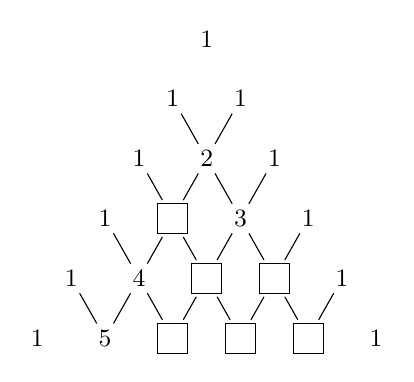
\begin{tikzpicture}[line width=0.4pt, font=\small,
  num/.style={inner sep=1.2pt},
  bx/.style={draw, line width=0.4pt, minimum size=3.8mm, inner sep=0pt},
  link/.style={line width=0.4pt, shorten >=1.2pt, shorten <=1.2pt}]
  % 행 k · 왼쪽부터 i 번째: x=(i-k/2)*0.86, y=-0.76k
  \node[num] (a00) at (0,0) {$1$};
  \node[num] (a10) at (-0.43,-0.76) {$1$};
  \node[num] (a11) at (0.43,-0.76) {$1$};
  \node[num] (a20) at (-0.86,-1.52) {$1$};
  \node[num] (a21) at (0,-1.52) {$2$};
  \node[num] (a22) at (0.86,-1.52) {$1$};
  \node[num] (a30) at (-1.29,-2.28) {$1$};
  \node[bx]  (a31) at (-0.43,-2.28) {};
  \node[num] (a32) at (0.43,-2.28) {$3$};
  \node[num] (a33) at (1.29,-2.28) {$1$};
  \node[num] (a40) at (-1.72,-3.04) {$1$};
  \node[num] (a41) at (-0.86,-3.04) {$4$};
  \node[bx]  (a42) at (0,-3.04) {};
  \node[bx]  (a43) at (0.86,-3.04) {};
  \node[num] (a44) at (1.72,-3.04) {$1$};
  \node[num] (a50) at (-2.15,-3.80) {$1$};
  \node[num] (a51) at (-1.29,-3.80) {$5$};
  \node[bx]  (a52) at (-0.43,-3.80) {};
  \node[bx]  (a53) at (0.43,-3.80) {};
  \node[bx]  (a54) at (1.29,-3.80) {};
  \node[num] (a55) at (2.15,-3.80) {$1$};
  % 이웃하는 두 수를 아래 수에 잇는 짧은 선(가장자리 1 에는 선이 없다 — 원문대로)
  \draw[link] (a10) -- (a21); \draw[link] (a11) -- (a21);
  \draw[link] (a20) -- (a31); \draw[link] (a21) -- (a31);
  \draw[link] (a21) -- (a32); \draw[link] (a22) -- (a32);
  \draw[link] (a30) -- (a41); \draw[link] (a31) -- (a41);
  \draw[link] (a31) -- (a42); \draw[link] (a32) -- (a42);
  \draw[link] (a32) -- (a43); \draw[link] (a33) -- (a43);
  \draw[link] (a40) -- (a51); \draw[link] (a41) -- (a51);
  \draw[link] (a41) -- (a52); \draw[link] (a42) -- (a52);
  \draw[link] (a42) -- (a53); \draw[link] (a43) -- (a53);
  \draw[link] (a43) -- (a54); \draw[link] (a44) -- (a54);
\end{tikzpicture}
}\end{minipage}\par
}\vspace{8mm}
\dmpassage{파스칼의 삼각형을 이용하여 다음 식을 전개하시오.}
\setcounter{dmproblemcount}{22}\dmpnum{30-23}{% id: 30-23
% book: 베이직쎈 확률과 통계 · 02 중복조합과 이항정리
% section: 개념 09 파스칼의 삼각형
% passage: 파스칼의 삼각형을 이용하여 다음 식을 전개하시오.
% figure: none
% answer: 
% answer_source: 
% variant_level: 0 (원본 전사)
% 이 파일은 build.mjs 가 items.json 에서 만든다. 고칠 때는 items.json 을 고친다.
\smash{\raisebox{1.5mm}{\dmkichul{베이직쎈 확률과 통계 30쪽 23번}}}
$(x+4)^4$
}\vspace{8mm}
\setcounter{dmproblemcount}{23}\dmpnum{30-24}{% id: 30-24
% book: 베이직쎈 확률과 통계 · 02 중복조합과 이항정리
% section: 개념 09 파스칼의 삼각형
% passage: 파스칼의 삼각형을 이용하여 다음 식을 전개하시오.
% figure: none
% answer: 
% answer_source: 
% variant_level: 0 (원본 전사)
% 이 파일은 build.mjs 가 items.json 에서 만든다. 고칠 때는 items.json 을 고친다.
\smash{\raisebox{1.5mm}{\dmkichul{베이직쎈 확률과 통계 30쪽 24번}}}
$(2a+b)^5$
}\vspace{8mm}
\dmpassage{다음을 ${}_n\mathrm{C}_r$ 꼴로 나타내시오.}
\setcounter{dmproblemcount}{24}\dmpnum{30-25}{% id: 30-25
% book: 베이직쎈 확률과 통계 · 02 중복조합과 이항정리
% section: 개념 09 파스칼의 삼각형
% passage: 다음을 ${}_n\mathrm{C}_r$ 꼴로 나타내시오.
% figure: none
% answer: 
% answer_source: 
% variant_level: 0 (원본 전사)
% 이 파일은 build.mjs 가 items.json 에서 만든다. 고칠 때는 items.json 을 고친다.
\smash{\raisebox{1.5mm}{\dmkichul{베이직쎈 확률과 통계 30쪽 25번}}}
${}_3\mathrm{C}_2+{}_3\mathrm{C}_3$
}\vspace{8mm}
\setcounter{dmproblemcount}{25}\dmpnum{30-26}{% id: 30-26
% book: 베이직쎈 확률과 통계 · 02 중복조합과 이항정리
% section: 개념 09 파스칼의 삼각형
% passage: 다음을 ${}_n\mathrm{C}_r$ 꼴로 나타내시오.
% figure: none
% answer: 
% answer_source: 
% variant_level: 0 (원본 전사)
% 이 파일은 build.mjs 가 items.json 에서 만든다. 고칠 때는 items.json 을 고친다.
\smash{\raisebox{1.5mm}{\dmkichul{베이직쎈 확률과 통계 30쪽 26번}}}
${}_5\mathrm{C}_1+{}_5\mathrm{C}_2$
}\vspace{8mm}
\setcounter{dmproblemcount}{26}\dmpnum{30-27}{% id: 30-27
% book: 베이직쎈 확률과 통계 · 02 중복조합과 이항정리
% section: 개념 09 파스칼의 삼각형
% passage: 다음을 ${}_n\mathrm{C}_r$ 꼴로 나타내시오.
% figure: none
% answer: 
% answer_source: 
% variant_level: 0 (원본 전사)
% 이 파일은 build.mjs 가 items.json 에서 만든다. 고칠 때는 items.json 을 고친다.
\smash{\raisebox{1.5mm}{\dmkichul{베이직쎈 확률과 통계 30쪽 27번}}}
${}_7\mathrm{C}_3+{}_7\mathrm{C}_4$
}\vspace{8mm}
\setcounter{dmproblemcount}{27}\dmpnum{30-28}{% id: 30-28
% book: 베이직쎈 확률과 통계 · 02 중복조합과 이항정리
% section: 개념 09 파스칼의 삼각형
% passage: 다음을 ${}_n\mathrm{C}_r$ 꼴로 나타내시오.
% figure: none
% answer: 
% answer_source: 
% variant_level: 0 (원본 전사)
% 이 파일은 build.mjs 가 items.json 에서 만든다. 고칠 때는 items.json 을 고친다.
\smash{\raisebox{1.5mm}{\dmkichul{베이직쎈 확률과 통계 30쪽 28번}}}
${}_2\mathrm{C}_0+{}_2\mathrm{C}_1+{}_3\mathrm{C}_2$
}\vspace{8mm}
\setcounter{dmproblemcount}{28}\dmpnum{30-29}{% id: 30-29
% book: 베이직쎈 확률과 통계 · 02 중복조합과 이항정리
% section: 개념 09 파스칼의 삼각형
% passage: 다음을 ${}_n\mathrm{C}_r$ 꼴로 나타내시오.
% figure: none
% answer: 
% answer_source: 
% variant_level: 0 (원본 전사)
% 이 파일은 build.mjs 가 items.json 에서 만든다. 고칠 때는 items.json 을 고친다.
\smash{\raisebox{1.5mm}{\dmkichul{베이직쎈 확률과 통계 30쪽 29번}}}
${}_5\mathrm{C}_2+{}_5\mathrm{C}_3+{}_6\mathrm{C}_4$
}\vspace{8mm}
\setcounter{dmproblemcount}{29}\dmpnum{30-30}{% id: 30-30
% book: 베이직쎈 확률과 통계 · 02 중복조합과 이항정리
% section: 개념 09 파스칼의 삼각형
% passage: 다음을 ${}_n\mathrm{C}_r$ 꼴로 나타내시오.
% figure: none
% answer: 
% answer_source: 
% variant_level: 0 (원본 전사)
% 이 파일은 build.mjs 가 items.json 에서 만든다. 고칠 때는 items.json 을 고친다.
\smash{\raisebox{1.5mm}{\dmkichul{베이직쎈 확률과 통계 30쪽 30번}}}
${}_6\mathrm{C}_2+{}_6\mathrm{C}_3+{}_7\mathrm{C}_2$
}\vspace{8mm}
\dmsection{유형 018 $(a+b)^n$의 전개식}
\setcounter{dmproblemcount}{0}\dmpnum{31-01}{% id: 31-01
% book: 베이직쎈 확률과 통계 · 02 중복조합과 이항정리
% section: 유형 018 $(a+b)^n$의 전개식
% figure: none
% answer: 
% answer_source: 
% variant_level: 0 (원본 전사)
% 이 파일은 build.mjs 가 items.json 에서 만든다. 고칠 때는 items.json 을 고친다.
\smash{\raisebox{1.5mm}{\dmkichul{베이직쎈 확률과 통계 31쪽 01번}}}
$(x+2y)^8$의 전개식에서 $x^6y^2$의 계수는?
\dmchoicesauto{}{$108$}{$110$}{$112$}{$114$}{$116$}
}\vspace{8mm}
\vspace{3mm}\setcounter{dmproblemcount}{1}\dmpnum{31-02}{% id: 31-02
% book: 베이직쎈 확률과 통계 · 02 중복조합과 이항정리
% section: 유형 018 $(a+b)^n$의 전개식
% figure: none
% answer: 
% answer_source: 
% variant_level: 0 (원본 전사)
% 이 파일은 build.mjs 가 items.json 에서 만든다. 고칠 때는 items.json 을 고친다.
\smash{\raisebox{4.5mm}{\dmkichul{베이직쎈 확률과 통계 31쪽 02번}}}
$\left(3x+\dfrac{1}{x^2}\right)^7$의 전개식에서 $\dfrac{1}{x^{11}}$의 계수를 구하시오.
}\vspace{8mm}
\vspace{3mm}\setcounter{dmproblemcount}{2}\dmpnum{31-03}{% id: 31-03
% book: 베이직쎈 확률과 통계 · 02 중복조합과 이항정리
% section: 유형 018 $(a+b)^n$의 전개식
% figure: none
% answer: 
% answer_source: 
% variant_level: 0 (원본 전사)
% 이 파일은 build.mjs 가 items.json 에서 만든다. 고칠 때는 items.json 을 고친다.
\smash{\raisebox{4.5mm}{\dmkichul{베이직쎈 확률과 통계 31쪽 03번}}}
$\left(\dfrac{a}{2}+b\right)^5$의 전개식에서 서로 다른 항의 개수는 $m$이고 $a^2b^3$의 계수는 $n$일 때, $mn$의 값은?
\dmchoicesauto{}{$15$}{$16$}{$17$}{$18$}{$19$}
}\vspace{8mm}
\setcounter{dmproblemcount}{3}\dmpnum{31-04}{% id: 31-04
% book: 베이직쎈 확률과 통계 · 02 중복조합과 이항정리
% section: 유형 018 $(a+b)^n$의 전개식
% figure: none
% answer: 
% answer_source: 
% variant_level: 0 (원본 전사)
% 이 파일은 build.mjs 가 items.json 에서 만든다. 고칠 때는 items.json 을 고친다.
\smash{\raisebox{1.5mm}{\dmkichul{베이직쎈 확률과 통계 31쪽 04번}}}
$(ax+1)^4$의 전개식에서 $x^3$의 계수가 $256$일 때, 상수 $a$의 값을 구하시오.
}\vspace{8mm}
\setcounter{dmproblemcount}{4}\dmpnum{31-05}{% id: 31-05
% book: 베이직쎈 확률과 통계 · 02 중복조합과 이항정리
% section: 유형 018 $(a+b)^n$의 전개식
% figure: none
% answer: 
% answer_source: 
% variant_level: 0 (원본 전사)
% 이 파일은 build.mjs 가 items.json 에서 만든다. 고칠 때는 items.json 을 고친다.
\smash{\raisebox{1.5mm}{\dmkichul{베이직쎈 확률과 통계 31쪽 05번}}}
$(x+a)^5$의 전개식에서 $x^3$의 계수가 $x^4$의 계수의 $4$배일 때, 상수 $a$의 값은? \dmcondfill{$a\ne 0$}{}
\dmchoicesauto{}{$1$}{$2$}{$3$}{$4$}{$5$}
}\vspace{8mm}
\dmsection{유형 019 이항계수의 활용}
\setcounter{dmproblemcount}{5}\dmpnum{31-06}{% id: 31-06
% book: 베이직쎈 확률과 통계 · 02 중복조합과 이항정리
% section: 유형 019 이항계수의 활용
% figure: none
% answer: 
% answer_source: 
% variant_level: 0 (원본 전사)
% 이 파일은 build.mjs 가 items.json 에서 만든다. 고칠 때는 items.json 을 고친다.
\smash{\raisebox{1.5mm}{\dmkichul{베이직쎈 확률과 통계 31쪽 06번}}}
$(1+x)(1-3x)^5$의 전개식에서 $x^3$의 계수는?
\dmchoicesauto{}{$-200$}{$-180$}{$-160$}{$160$}{$180$}
}\vspace{8mm}
\vspace{3mm}\setcounter{dmproblemcount}{6}\dmpnum{31-07}{% id: 31-07
% book: 베이직쎈 확률과 통계 · 02 중복조합과 이항정리
% section: 유형 019 이항계수의 활용
% figure: none
% answer: 
% answer_source: 
% variant_level: 0 (원본 전사)
% 이 파일은 build.mjs 가 items.json 에서 만든다. 고칠 때는 items.json 을 고친다.
\smash{\raisebox{4.5mm}{\dmkichul{베이직쎈 확률과 통계 31쪽 07번}}}
$(x^2-4)\left(x+\dfrac{3}{x}\right)^4$의 전개식에서 상수항을 구하시오.
}\vspace{8mm}
\setcounter{dmproblemcount}{7}\dmpnum{32-08}{% id: 32-08
% book: 베이직쎈 확률과 통계 · 02 중복조합과 이항정리
% section: 유형 019 이항계수의 활용
% figure: none
% answer: 
% answer_source: 
% variant_level: 0 (원본 전사)
% 이 파일은 build.mjs 가 items.json 에서 만든다. 고칠 때는 items.json 을 고친다.
\smash{\raisebox{1.5mm}{\dmkichul{베이직쎈 확률과 통계 32쪽 08번}}}
$(ax+2)(x+1)^6$의 전개식에서 $x^4$의 계수가 $90$일 때, 상수 $a$의 값을 구하시오.
}\vspace{8mm}
\dmsection{유형 020 이항계수의 성질}
\vspace{3mm}\setcounter{dmproblemcount}{8}\dmpnum{32-09}{% id: 32-09
% book: 베이직쎈 확률과 통계 · 02 중복조합과 이항정리
% section: 유형 020 이항계수의 성질
% figure: none
% answer: 
% answer_source: 
% variant_level: 0 (원본 전사)
% 이 파일은 build.mjs 가 items.json 에서 만든다. 고칠 때는 items.json 을 고친다.
\smash{\raisebox{4.5mm}{\dmkichul{베이직쎈 확률과 통계 32쪽 09번}}}
$\dfrac{{}_{30}\mathrm{C}_0+{}_{30}\mathrm{C}_1+{}_{30}\mathrm{C}_2+\cdots+{}_{30}\mathrm{C}_{30}}{{}_{30}\mathrm{C}_0+{}_{30}\mathrm{C}_2+{}_{30}\mathrm{C}_4+\cdots+{}_{30}\mathrm{C}_{30}}$의 값을 구하시오.
}\vspace{8mm}
\setcounter{dmproblemcount}{9}\dmpnum{32-10}{% id: 32-10
% book: 베이직쎈 확률과 통계 · 02 중복조합과 이항정리
% section: 유형 020 이항계수의 성질
% figure: none
% answer: 
% answer_source: 
% variant_level: 0 (원본 전사)
% 이 파일은 build.mjs 가 items.json 에서 만든다. 고칠 때는 items.json 을 고친다.
\smash{\raisebox{1.5mm}{\dmkichul{베이직쎈 확률과 통계 32쪽 10번}}}
옳은 것만을 \textbf{보기}에서 있는 대로 고른 것은? \bogi{ㄱ. ${}_{24}\mathrm{C}_0+{}_{24}\mathrm{C}_1+{}_{24}\mathrm{C}_2+\cdots+{}_{24}\mathrm{C}_{24}=2^{24}$\\ ㄴ. ${}_{13}\mathrm{C}_0-{}_{13}\mathrm{C}_1+{}_{13}\mathrm{C}_2-\cdots-{}_{13}\mathrm{C}_{13}=2^{12}$\\ ㄷ. ${}_8\mathrm{C}_0+{}_8\mathrm{C}_2+{}_8\mathrm{C}_4+{}_8\mathrm{C}_6+{}_8\mathrm{C}_8={}_8\mathrm{C}_1+{}_8\mathrm{C}_3+{}_8\mathrm{C}_5+{}_8\mathrm{C}_7$}
\dmchoicesauto{}{ㄱ}{ㄴ}{ㄱ, ㄷ}{ㄴ, ㄷ}{ㄱ, ㄴ, ㄷ}
}\vspace{8mm}
\setcounter{dmproblemcount}{10}\dmpnum{32-11}{% id: 32-11
% book: 베이직쎈 확률과 통계 · 02 중복조합과 이항정리
% section: 유형 020 이항계수의 성질
% figure: none
% answer: 
% answer_source: 
% variant_level: 0 (원본 전사)
% 이 파일은 build.mjs 가 items.json 에서 만든다. 고칠 때는 items.json 을 고친다.
\smash{\raisebox{1.5mm}{\dmkichul{베이직쎈 확률과 통계 32쪽 11번}}}
${}_{21}\mathrm{C}_0+{}_{21}\mathrm{C}_1+{}_{21}\mathrm{C}_2+\cdots+{}_{21}\mathrm{C}_{10}$의 값은?
\dmchoicesauto{}{$2^{17}$}{$2^{18}$}{$2^{19}$}{$2^{20}$}{$2^{21}$}
}\vspace{8mm}
\setcounter{dmproblemcount}{11}\dmpnum{32-12}{% id: 32-12
% book: 베이직쎈 확률과 통계 · 02 중복조합과 이항정리
% section: 유형 020 이항계수의 성질
% figure: none
% answer: 
% answer_source: 
% variant_level: 0 (원본 전사)
% 이 파일은 build.mjs 가 items.json 에서 만든다. 고칠 때는 items.json 을 고친다.
\smash{\raisebox{1.5mm}{\dmkichul{베이직쎈 확률과 통계 32쪽 12번}}}
${}_n\mathrm{C}_1+{}_n\mathrm{C}_2+{}_n\mathrm{C}_3+\cdots+{}_n\mathrm{C}_n=511$을 만족시키는 자연수 $n$의 값은?
\dmchoicesauto{}{$7$}{$8$}{$9$}{$10$}{$11$}
}\vspace{8mm}
\setcounter{dmproblemcount}{12}\dmpnum{32-13}{% id: 32-13
% book: 베이직쎈 확률과 통계 · 02 중복조합과 이항정리
% section: 유형 020 이항계수의 성질
% figure: none
% answer: 
% answer_source: 
% variant_level: 0 (원본 전사)
% 이 파일은 build.mjs 가 items.json 에서 만든다. 고칠 때는 items.json 을 고친다.
\smash{\raisebox{1.5mm}{\dmkichul{베이직쎈 확률과 통계 32쪽 13번}}}
${}_{15}\mathrm{C}_0+{}_{15}\mathrm{C}_1\cdot 7+{}_{15}\mathrm{C}_2\cdot 7^2+\cdots+{}_{15}\mathrm{C}_{15}\cdot 7^{15}=2^n$을 만족시키는 자연수 $n$의 값을 구하시오.
}\vspace{8mm}
\setcounter{dmproblemcount}{13}\dmpnum{32-14}{% id: 32-14
% book: 베이직쎈 확률과 통계 · 02 중복조합과 이항정리
% section: 유형 020 이항계수의 성질
% figure: none
% answer: 
% answer_source: 
% variant_level: 0 (원본 전사)
% 이 파일은 build.mjs 가 items.json 에서 만든다. 고칠 때는 items.json 을 고친다.
\smash{\raisebox{1.5mm}{\dmkichul{베이직쎈 확률과 통계 32쪽 14번}}}
$n$이 홀수일 때, 부등식\par\smallskip\dispeq{$1000<{}_n\mathrm{C}_1+{}_n\mathrm{C}_3+{}_n\mathrm{C}_5+\cdots+{}_n\mathrm{C}_n<2000$}\par\smallskip\noindent 을 만족시키는 $n$의 값은?
\dmchoicesauto{}{$9$}{$11$}{$13$}{$15$}{$17$}
}\vspace{8mm}
\dmsection{유형 021 이항계수의 합}
\setcounter{dmproblemcount}{14}\dmpnum{33-15}{% id: 33-15
% book: 베이직쎈 확률과 통계 · 02 중복조합과 이항정리
% section: 유형 021 이항계수의 합
% figure: none
% answer: 
% answer_source: 
% variant_level: 0 (원본 전사)
% 이 파일은 build.mjs 가 items.json 에서 만든다. 고칠 때는 items.json 을 고친다.
\smash{\raisebox{1.5mm}{\dmkichul{베이직쎈 확률과 통계 33쪽 15번}}}
${}_{n-1}\mathrm{C}_2+{}_{n-1}\mathrm{C}_3={}_n\mathrm{C}_5$를 만족시키는 자연수 $n$의 값은?
\dmchoicesauto{}{$5$}{$6$}{$7$}{$8$}{$9$}
}\vspace{8mm}
\setcounter{dmproblemcount}{15}\dmpnum{33-16}{% id: 33-16
% book: 베이직쎈 확률과 통계 · 02 중복조합과 이항정리
% section: 유형 021 이항계수의 합
% figure: tikz:fig-33-16
% answer: 
% answer_source: 
% variant_level: 0 (원본 전사)
% 이 파일은 build.mjs 가 items.json 에서 만든다. 고칠 때는 items.json 을 고친다.
\smash{\raisebox{1.5mm}{\dmkichul{베이직쎈 확률과 통계 33쪽 16번}}}
다음은 아래 그림의 색칠한 부분에 있는 수의 합을 구하는 과정이다. ㈎$\sim$㈒에 알맞은 것으로 옳지 \underline{않은} 것은? 
\par\smallskip\begin{center}\resizebox{\ifdim\width>\linewidth\linewidth\else\width\fi}{!}{% 33-16(인쇄 33쪽) — 이항계수로 나타낸 파스칼의 삼각형 5단계까지와 색칠한 띠(₂C₀, ₂C₁ 에서 ₃C₂, ₄C₃, ₅C₄ 로 꺾인 띠).
% 스캔 화질이 낮아 TikZ 로 다시 그림. 색칠한 자리는 원문과 같고, 각 칸의 값(수)은 원문에도 없으므로 적지 않는다.
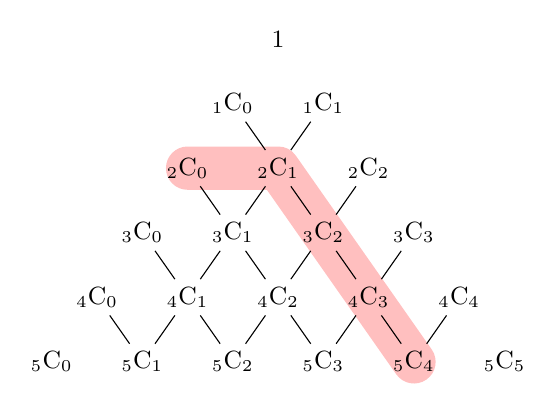
\begin{tikzpicture}[line width=0.4pt, font=\small,
  num/.style={inner sep=1.2pt},
  link/.style={line width=0.4pt, shorten >=8pt, shorten <=8pt}]
  % 행 k · 왼쪽부터 i 번째: x=(i-k/2)*1.15, y=-0.82k
  \coordinate (a00) at (0,0);
  \coordinate (a10) at (-0.575,-0.82); \coordinate (a11) at (0.575,-0.82);
  \coordinate (a20) at (-1.15,-1.64); \coordinate (a21) at (0,-1.64); \coordinate (a22) at (1.15,-1.64);
  \coordinate (a30) at (-1.725,-2.46); \coordinate (a31) at (-0.575,-2.46);
  \coordinate (a32) at (0.575,-2.46); \coordinate (a33) at (1.725,-2.46);
  \coordinate (a40) at (-2.3,-3.28); \coordinate (a41) at (-1.15,-3.28); \coordinate (a42) at (0,-3.28);
  \coordinate (a43) at (1.15,-3.28); \coordinate (a44) at (2.3,-3.28);
  \coordinate (a50) at (-2.875,-4.1); \coordinate (a51) at (-1.725,-4.1); \coordinate (a52) at (-0.575,-4.1);
  \coordinate (a53) at (0.575,-4.1); \coordinate (a54) at (1.725,-4.1); \coordinate (a55) at (2.875,-4.1);
  % 색칠한 띠
  \draw[line width=5.5mm, red!25, line cap=round, line join=round] (a20) -- (a21) -- (a54);
  % 이웃하는 두 수를 아래 수에 잇는 짧은 선(가장자리에는 선이 없다 — 원문대로)
  \draw[link] (a10) -- (a21); \draw[link] (a11) -- (a21);
  \draw[link] (a20) -- (a31); \draw[link] (a21) -- (a31);
  \draw[link] (a21) -- (a32); \draw[link] (a22) -- (a32);
  \draw[link] (a30) -- (a41); \draw[link] (a31) -- (a41);
  \draw[link] (a31) -- (a42); \draw[link] (a32) -- (a42);
  \draw[link] (a32) -- (a43); \draw[link] (a33) -- (a43);
  \draw[link] (a40) -- (a51); \draw[link] (a41) -- (a51);
  \draw[link] (a41) -- (a52); \draw[link] (a42) -- (a52);
  \draw[link] (a42) -- (a53); \draw[link] (a43) -- (a53);
  \draw[link] (a43) -- (a54); \draw[link] (a44) -- (a54);
  \node[num] at (a00) {$1$};
  \node[num] at (a10) {${}_1\mathrm{C}_0$}; \node[num] at (a11) {${}_1\mathrm{C}_1$};
  \node[num] at (a20) {${}_2\mathrm{C}_0$}; \node[num] at (a21) {${}_2\mathrm{C}_1$}; \node[num] at (a22) {${}_2\mathrm{C}_2$};
  \node[num] at (a30) {${}_3\mathrm{C}_0$}; \node[num] at (a31) {${}_3\mathrm{C}_1$};
  \node[num] at (a32) {${}_3\mathrm{C}_2$}; \node[num] at (a33) {${}_3\mathrm{C}_3$};
  \node[num] at (a40) {${}_4\mathrm{C}_0$}; \node[num] at (a41) {${}_4\mathrm{C}_1$}; \node[num] at (a42) {${}_4\mathrm{C}_2$};
  \node[num] at (a43) {${}_4\mathrm{C}_3$}; \node[num] at (a44) {${}_4\mathrm{C}_4$};
  \node[num] at (a50) {${}_5\mathrm{C}_0$}; \node[num] at (a51) {${}_5\mathrm{C}_1$}; \node[num] at (a52) {${}_5\mathrm{C}_2$};
  \node[num] at (a53) {${}_5\mathrm{C}_3$}; \node[num] at (a54) {${}_5\mathrm{C}_4$}; \node[num] at (a55) {${}_5\mathrm{C}_5$};
\end{tikzpicture}
}\end{center}
\noindent \exprbox{${}_2\mathrm{C}_0+{}_2\mathrm{C}_1+{}_3\mathrm{C}_2+{}_4\mathrm{C}_3+{}_5\mathrm{C}_4$\\ $=\fbox{㈎}+{}_3\mathrm{C}_2+{}_4\mathrm{C}_3+{}_5\mathrm{C}_4$\\ $=\fbox{㈏}+{}_4\mathrm{C}_3+{}_5\mathrm{C}_4$\\ $=\fbox{㈐}+{}_5\mathrm{C}_4$\\ $=\fbox{㈑}$\\ $=\fbox{㈒}$}
\dmchoicesauto{}{㈎ ${}_3\mathrm{C}_1$}{㈏ ${}_4\mathrm{C}_2$}{㈐ ${}_5\mathrm{C}_3$}{㈑ ${}_6\mathrm{C}_5$}{㈒ $15$}
}\vspace{8mm}
\setcounter{dmproblemcount}{16}\dmpnum{33-17}{% id: 33-17
% book: 베이직쎈 확률과 통계 · 02 중복조합과 이항정리
% section: 유형 021 이항계수의 합
% figure: tikz:fig-33-17
% answer: 
% answer_source: 
% variant_level: 0 (원본 전사)
% 이 파일은 build.mjs 가 items.json 에서 만든다. 고칠 때는 items.json 을 고친다.
\smash{\raisebox{1.5mm}{\dmkichul{베이직쎈 확률과 통계 33쪽 17번}}}
다음 그림의 색칠한 부분에 있는 수의 합을 구하시오.
\par\smallskip\begin{center}\resizebox{\ifdim\width>\linewidth\linewidth\else\width\fi}{!}{% 33-17(인쇄 33쪽) — 이항계수로 나타낸 파스칼의 삼각형 6단계까지와 색칠한 띠(₃C₃, ₄C₃, ₅C₃, ₆C₃ 를 잇는 비스듬한 띠).
% 스캔 화질이 낮아 TikZ 로 다시 그림. 색칠한 자리는 원문과 같고, 각 칸의 값(수)은 원문에도 없으므로 적지 않는다.
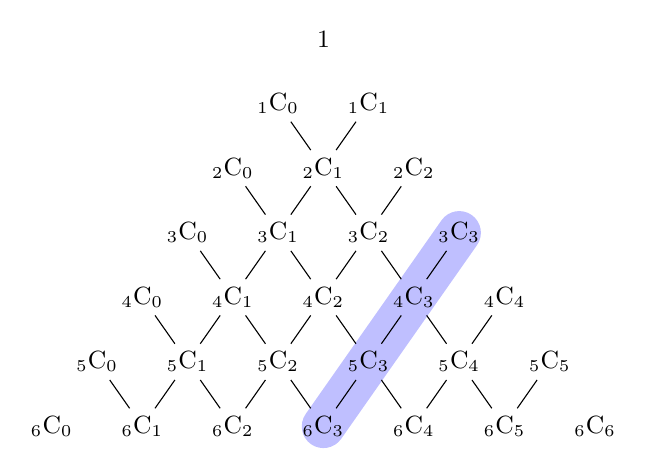
\begin{tikzpicture}[line width=0.4pt, font=\small,
  num/.style={inner sep=1.2pt},
  link/.style={line width=0.4pt, shorten >=8pt, shorten <=8pt}]
  % 행 k · 왼쪽부터 i 번째: x=(i-k/2)*1.15, y=-0.82k
  \coordinate (a00) at (0,0);
  \coordinate (a10) at (-0.575,-0.82); \coordinate (a11) at (0.575,-0.82);
  \coordinate (a20) at (-1.15,-1.64); \coordinate (a21) at (0,-1.64); \coordinate (a22) at (1.15,-1.64);
  \coordinate (a30) at (-1.725,-2.46); \coordinate (a31) at (-0.575,-2.46);
  \coordinate (a32) at (0.575,-2.46); \coordinate (a33) at (1.725,-2.46);
  \coordinate (a40) at (-2.3,-3.28); \coordinate (a41) at (-1.15,-3.28); \coordinate (a42) at (0,-3.28);
  \coordinate (a43) at (1.15,-3.28); \coordinate (a44) at (2.3,-3.28);
  \coordinate (a50) at (-2.875,-4.1); \coordinate (a51) at (-1.725,-4.1); \coordinate (a52) at (-0.575,-4.1);
  \coordinate (a53) at (0.575,-4.1); \coordinate (a54) at (1.725,-4.1); \coordinate (a55) at (2.875,-4.1);
  \coordinate (a60) at (-3.45,-4.92); \coordinate (a61) at (-2.3,-4.92); \coordinate (a62) at (-1.15,-4.92);
  \coordinate (a63) at (0,-4.92); \coordinate (a64) at (1.15,-4.92); \coordinate (a65) at (2.3,-4.92);
  \coordinate (a66) at (3.45,-4.92);
  % 색칠한 띠
  \draw[line width=5.5mm, blue!25, line cap=round] (a33) -- (a63);
  % 이웃하는 두 수를 아래 수에 잇는 짧은 선(가장자리에는 선이 없다 — 원문대로)
  \draw[link] (a10) -- (a21); \draw[link] (a11) -- (a21);
  \draw[link] (a20) -- (a31); \draw[link] (a21) -- (a31);
  \draw[link] (a21) -- (a32); \draw[link] (a22) -- (a32);
  \draw[link] (a30) -- (a41); \draw[link] (a31) -- (a41);
  \draw[link] (a31) -- (a42); \draw[link] (a32) -- (a42);
  \draw[link] (a32) -- (a43); \draw[link] (a33) -- (a43);
  \draw[link] (a40) -- (a51); \draw[link] (a41) -- (a51);
  \draw[link] (a41) -- (a52); \draw[link] (a42) -- (a52);
  \draw[link] (a42) -- (a53); \draw[link] (a43) -- (a53);
  \draw[link] (a43) -- (a54); \draw[link] (a44) -- (a54);
  \draw[link] (a50) -- (a61); \draw[link] (a51) -- (a61);
  \draw[link] (a51) -- (a62); \draw[link] (a52) -- (a62);
  \draw[link] (a52) -- (a63); \draw[link] (a53) -- (a63);
  \draw[link] (a53) -- (a64); \draw[link] (a54) -- (a64);
  \draw[link] (a54) -- (a65); \draw[link] (a55) -- (a65);
  \node[num] at (a00) {$1$};
  \node[num] at (a10) {${}_1\mathrm{C}_0$}; \node[num] at (a11) {${}_1\mathrm{C}_1$};
  \node[num] at (a20) {${}_2\mathrm{C}_0$}; \node[num] at (a21) {${}_2\mathrm{C}_1$}; \node[num] at (a22) {${}_2\mathrm{C}_2$};
  \node[num] at (a30) {${}_3\mathrm{C}_0$}; \node[num] at (a31) {${}_3\mathrm{C}_1$};
  \node[num] at (a32) {${}_3\mathrm{C}_2$}; \node[num] at (a33) {${}_3\mathrm{C}_3$};
  \node[num] at (a40) {${}_4\mathrm{C}_0$}; \node[num] at (a41) {${}_4\mathrm{C}_1$}; \node[num] at (a42) {${}_4\mathrm{C}_2$};
  \node[num] at (a43) {${}_4\mathrm{C}_3$}; \node[num] at (a44) {${}_4\mathrm{C}_4$};
  \node[num] at (a50) {${}_5\mathrm{C}_0$}; \node[num] at (a51) {${}_5\mathrm{C}_1$}; \node[num] at (a52) {${}_5\mathrm{C}_2$};
  \node[num] at (a53) {${}_5\mathrm{C}_3$}; \node[num] at (a54) {${}_5\mathrm{C}_4$}; \node[num] at (a55) {${}_5\mathrm{C}_5$};
  \node[num] at (a60) {${}_6\mathrm{C}_0$}; \node[num] at (a61) {${}_6\mathrm{C}_1$}; \node[num] at (a62) {${}_6\mathrm{C}_2$};
  \node[num] at (a63) {${}_6\mathrm{C}_3$}; \node[num] at (a64) {${}_6\mathrm{C}_4$}; \node[num] at (a65) {${}_6\mathrm{C}_5$};
  \node[num] at (a66) {${}_6\mathrm{C}_6$};
\end{tikzpicture}
}\end{center}
}\vspace{8mm}
\setcounter{dmproblemcount}{17}\dmpnum{33-18}{% id: 33-18
% book: 베이직쎈 확률과 통계 · 02 중복조합과 이항정리
% section: 유형 021 이항계수의 합
% figure: none
% answer: 
% answer_source: 
% variant_level: 0 (원본 전사)
% 이 파일은 build.mjs 가 items.json 에서 만든다. 고칠 때는 items.json 을 고친다.
\smash{\raisebox{1.5mm}{\dmkichul{베이직쎈 확률과 통계 33쪽 18번}}}
다음 중 ${}_3\mathrm{C}_0+{}_4\mathrm{C}_1+{}_5\mathrm{C}_2+\cdots+{}_9\mathrm{C}_6$의 값과 같은 것은?
\dmchoicesauto{}{${}_{10}\mathrm{C}_3$}{${}_{10}\mathrm{C}_4$}{${}_{10}\mathrm{C}_5$}{${}_{11}\mathrm{C}_4$}{${}_{11}\mathrm{C}_5$}
}\vspace{8mm}
\setcounter{dmproblemcount}{18}\dmpnum{33-19}{% id: 33-19
% book: 베이직쎈 확률과 통계 · 02 중복조합과 이항정리
% section: 유형 021 이항계수의 합
% figure: none
% answer: 
% answer_source: 
% variant_level: 0 (원본 전사)
% 이 파일은 build.mjs 가 items.json 에서 만든다. 고칠 때는 items.json 을 고친다.
\smash{\raisebox{1.5mm}{\dmkichul{베이직쎈 확률과 통계 33쪽 19번}}}
${}_2\mathrm{C}_2+{}_3\mathrm{C}_2+{}_4\mathrm{C}_2+\cdots+{}_8\mathrm{C}_2$의 값을 구하시오.
}\vspace{8mm}
\setcounter{dmproblemcount}{19}\dmpnum{33-20}{% id: 33-20
% book: 베이직쎈 확률과 통계 · 02 중복조합과 이항정리
% section: 유형 021 이항계수의 합
% figure: none
% answer: 
% answer_source: 
% variant_level: 0 (원본 전사)
% 이 파일은 build.mjs 가 items.json 에서 만든다. 고칠 때는 items.json 을 고친다.
\smash{\raisebox{1.5mm}{\dmkichul{베이직쎈 확률과 통계 33쪽 20번}}}
다음 중 ${}_9\mathrm{C}_1+{}_{10}\mathrm{C}_2+{}_{11}\mathrm{C}_3$의 값과 같은 것은?
\begin{choices32}{${}_{11}\mathrm{C}_3-1$}{${}_{11}\mathrm{C}_3$}{${}_{12}\mathrm{C}_3-1$}{${}_{12}\mathrm{C}_3$}{${}_{12}\mathrm{C}_4$}\end{choices32}
}\vspace{8mm}
\dmsection{실전 감각 UP}
\setcounter{dmproblemcount}{0}\dmpnum{34-01}{% id: 34-01
% book: 베이직쎈 확률과 통계 · 02 중복조합과 이항정리
% section: 실전 감각 UP
% figure: crop:fig-34-01.jpg
% answer: 
% answer_source: 
% variant_level: 0 (원본 전사)
% 이 파일은 build.mjs 가 items.json 에서 만든다. 고칠 때는 items.json 을 고친다.
\smash{\raisebox{1.5mm}{\dmkichul{베이직쎈 확률과 통계 34쪽 01번}}}
\noindent\begin{minipage}[t]{0.58\linewidth}\vspace{0pt}\raggedright 오른쪽 그림은 어느 음료 가게의 메뉴판이다. 선희가 이 가게에서 메뉴판에 있는 음료 중 7개의 음료를 주문하는 경우의 수는?\end{minipage}\hfill\begin{minipage}[t]{0.4\linewidth}\vspace{0pt}\centering 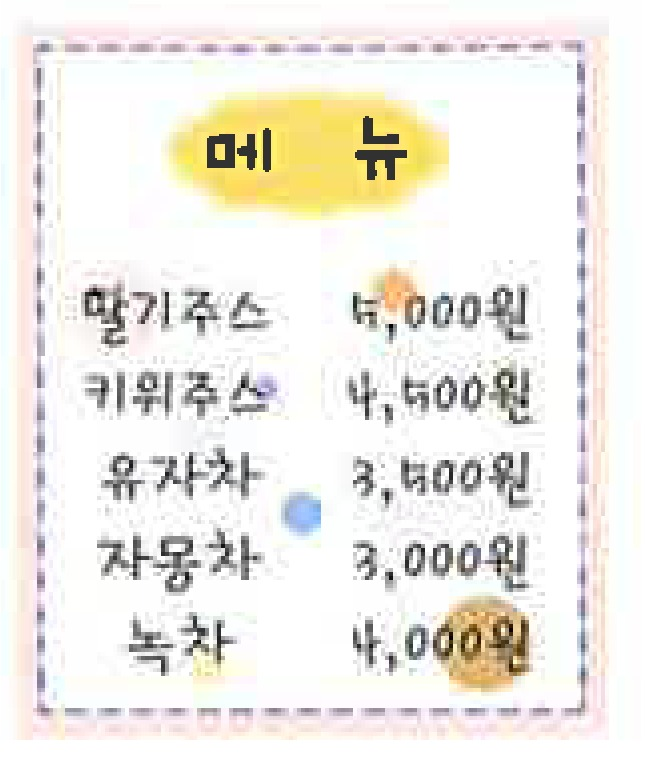
\includegraphics[width=0.92\linewidth]{figures/fig-34-01.jpg}\end{minipage}\par
\dmchoicesauto{}{$170$}{$210$}{$250$}{$290$}{$330$}
}\vspace{8mm}
\setcounter{dmproblemcount}{1}\dmpnum{34-02}{% id: 34-02
% book: 베이직쎈 확률과 통계 · 02 중복조합과 이항정리
% section: 실전 감각 UP
% figure: none
% answer: 
% answer_source: 
% variant_level: 0 (원본 전사)
% 이 파일은 build.mjs 가 items.json 에서 만든다. 고칠 때는 items.json 을 고친다.
\smash{\raisebox{1.5mm}{\dmkichul{베이직쎈 확률과 통계 34쪽 02번 · 꼭 나와요}}}
같은 종류의 공책 11권을 4명의 학생에게 나누어 주려고 한다. 각 학생이 적어도 2권의 공책을 받게 하려고 할 때, 공책을 나누어 주는 경우의 수는?
\dmchoicesauto{}{$12$}{$16$}{$20$}{$24$}{$28$}
}\vspace{8mm}
\setcounter{dmproblemcount}{2}\dmpnum{34-03}{% id: 34-03
% book: 베이직쎈 확률과 통계 · 02 중복조합과 이항정리
% section: 실전 감각 UP
% figure: none
% answer: 
% answer_source: 
% variant_level: 0 (원본 전사)
% 이 파일은 build.mjs 가 items.json 에서 만든다. 고칠 때는 items.json 을 고친다.
\smash{\raisebox{1.5mm}{\dmkichul{베이직쎈 확률과 통계 34쪽 03번}}}
다항식 $(a+b+c)^n$의 전개식에서 서로 다른 항의 개수가 $45$일 때, 자연수 $n$의 값은?
\dmchoicesauto{}{$5$}{$6$}{$7$}{$8$}{$9$}
}\vspace{8mm}
\setcounter{dmproblemcount}{3}\dmpnum{34-04}{% id: 34-04
% book: 베이직쎈 확률과 통계 · 02 중복조합과 이항정리
% section: 실전 감각 UP
% figure: none
% answer: 
% answer_source: 
% variant_level: 0 (원본 전사)
% 이 파일은 build.mjs 가 items.json 에서 만든다. 고칠 때는 items.json 을 고친다.
\smash{\raisebox{1.5mm}{\dmkichul{베이직쎈 확률과 통계 34쪽 04번}}}
방정식 $x+y+z=17$을 만족시키는 음이 아닌 홀수 $x$, $y$, $z$의 순서쌍 $(x{,}\mkern3mu\mathopen{}y{,}\mkern3mu\mathopen{}z)$의 개수는?
\dmchoicesauto{}{$32$}{$36$}{$40$}{$44$}{$48$}
}\vspace{8mm}
\setcounter{dmproblemcount}{4}\dmpnum{34-05}{% id: 34-05
% book: 베이직쎈 확률과 통계 · 02 중복조합과 이항정리
% section: 실전 감각 UP
% figure: none
% answer: 
% answer_source: 
% variant_level: 0 (원본 전사)
% 이 파일은 build.mjs 가 items.json 에서 만든다. 고칠 때는 items.json 을 고친다.
\smash{\raisebox{1.5mm}{\dmkichul{베이직쎈 확률과 통계 34쪽 05번}}}
$3\le a\le b\le c<9$를 만족시키는 세 자연수 $a$, $b$, $c$의 순서쌍 $(a{,}\mkern3mu\mathopen{}b{,}\mkern3mu\mathopen{}c)$의 개수는?
\dmchoicesauto{}{$56$}{$72$}{$88$}{$104$}{$120$}
}\vspace{8mm}
\vspace{3mm}\setcounter{dmproblemcount}{5}\dmpnum{34-06}{% id: 34-06
% book: 베이직쎈 확률과 통계 · 02 중복조합과 이항정리
% section: 실전 감각 UP
% figure: none
% answer: 
% answer_source: 
% variant_level: 0 (원본 전사)
% 이 파일은 build.mjs 가 items.json 에서 만든다. 고칠 때는 items.json 을 고친다.
\smash{\raisebox{4.5mm}{\dmkichul{베이직쎈 확률과 통계 34쪽 06번 · 꼭 나와요}}}
$\left(ax-\dfrac{2}{x}\right)^6$의 전개식에서 $x^2$의 계수가 $960$일 때, 양수 $a$의 값은?
\begin{choicesii}{\rule[-3ex]{0pt}{8ex}$\dfrac{1}{2}$}{\rule[-3ex]{0pt}{8ex}$1$}{\rule[-3ex]{0pt}{8ex}$\dfrac{3}{2}$}{\rule[-3ex]{0pt}{8ex}$2$}{\rule[-3ex]{0pt}{8ex}$\dfrac{5}{2}$}\end{choicesii}
}\vspace{8mm}
\setcounter{dmproblemcount}{6}\dmpnum{34-07}{% id: 34-07
% book: 베이직쎈 확률과 통계 · 02 중복조합과 이항정리
% section: 실전 감각 UP
% figure: none
% answer: 
% answer_source: 
% variant_level: 0 (원본 전사)
% 이 파일은 build.mjs 가 items.json 에서 만든다. 고칠 때는 items.json 을 고친다.
\smash{\raisebox{1.5mm}{\dmkichul{베이직쎈 확률과 통계 34쪽 07번}}}
$(x-y)(3x+2y)^5$의 전개식에서 $x^2y^4$의 계수는?
\dmchoicesauto{}{$-600$}{$-480$}{$-360$}{$-240$}{$-120$}
}\vspace{8mm}
\setcounter{dmproblemcount}{7}\dmpnum{35-08}{% id: 35-08
% book: 베이직쎈 확률과 통계 · 02 중복조합과 이항정리
% section: 실전 감각 UP
% figure: none
% answer: 
% answer_source: 
% variant_level: 0 (원본 전사)
% 이 파일은 build.mjs 가 items.json 에서 만든다. 고칠 때는 items.json 을 고친다.
\smash{\raisebox{1.5mm}{\dmkichul{베이직쎈 확률과 통계 35쪽 08번}}}
다음 중\par\smallskip\dispeq{${}_{10}\mathrm{C}_1\cdot 5+{}_{10}\mathrm{C}_2\cdot 5^2+{}_{10}\mathrm{C}_3\cdot 5^3+\cdots+{}_{10}\mathrm{C}_{10}\cdot 5^{10}$}\par\smallskip\noindent 의 값과 같은 것은?
\dmchoicesauto{}{$5^{10}-1$}{$5^{10}$}{$5^{10}+1$}{$6^{10}-1$}{$6^{10}$}
}\vspace{8mm}
\setcounter{dmproblemcount}{8}\dmpnum{35-09}{% id: 35-09
% book: 베이직쎈 확률과 통계 · 02 중복조합과 이항정리
% section: 실전 감각 UP
% figure: none
% answer: 
% answer_source: 
% variant_level: 0 (원본 전사)
% 이 파일은 build.mjs 가 items.json 에서 만든다. 고칠 때는 items.json 을 고친다.
\smash{\raisebox{1.5mm}{\dmkichul{베이직쎈 확률과 통계 35쪽 09번 · 꼭 나와요}}}
부등식 $50<{}_n\mathrm{C}_1+{}_n\mathrm{C}_2+{}_n\mathrm{C}_3+\cdots+{}_n\mathrm{C}_n<100$을 만족시키는 자연수 $n$의 값은?
\dmchoicesauto{}{$4$}{$5$}{$6$}{$7$}{$8$}
}\vspace{8mm}
\setcounter{dmproblemcount}{9}\dmpnum{35-10}{% id: 35-10
% book: 베이직쎈 확률과 통계 · 02 중복조합과 이항정리
% section: 실전 감각 UP
% figure: none
% answer: 
% answer_source: 
% variant_level: 0 (원본 전사)
% 이 파일은 build.mjs 가 items.json 에서 만든다. 고칠 때는 items.json 을 고친다.
\smash{\raisebox{1.5mm}{\dmkichul{베이직쎈 확률과 통계 35쪽 10번 · 서답형 · 서술형}}}
사과 6개, 귤 4개를 3명의 학생에게 나누어 주는 경우의 수를 구하시오. \dmcondfill{같은 종류의 과일은 서로 구별하지 않고, 과일을 받지 못하는 학생이 있을 수 있다.}{}
}\vspace{8mm}
\setcounter{dmproblemcount}{10}\dmpnum{35-11}{% id: 35-11
% book: 베이직쎈 확률과 통계 · 02 중복조합과 이항정리
% section: 실전 감각 UP
% figure: none
% answer: 
% answer_source: 
% variant_level: 0 (원본 전사)
% 이 파일은 build.mjs 가 items.json 에서 만든다. 고칠 때는 items.json 을 고친다.
\smash{\raisebox{1.5mm}{\dmkichul{베이직쎈 확률과 통계 35쪽 11번 · 서답형}}}
빨간색, 초록색, 파란색, 노란색 컵 중에서 7개의 컵을 사려고 한다. 빨간색 컵은 2개 이상, 파란색 컵은 3개 이상 사는 경우의 수를 구하시오. \dmcondfill{같은 색의 컵은 서로 구별하지 않고, 사지 않는 색의 컵이 있을 수 있다.}{}
}\vspace{8mm}
\setcounter{dmproblemcount}{11}\dmpnum{35-12}{% id: 35-12
% book: 베이직쎈 확률과 통계 · 02 중복조합과 이항정리
% section: 실전 감각 UP
% figure: none
% answer: 
% answer_source: 
% variant_level: 0 (원본 전사)
% 이 파일은 build.mjs 가 items.json 에서 만든다. 고칠 때는 items.json 을 고친다.
\smash{\raisebox{1.5mm}{\dmkichul{베이직쎈 확률과 통계 35쪽 12번 · 서답형 · 서술형}}}
부등식 $2<a+b+c+d\le 4$를 만족시키는 음이 아닌 정수 $a$, $b$, $c$, $d$의 순서쌍 $(a{,}\mkern3mu\mathopen{}b{,}\mkern3mu\mathopen{}c{,}\mkern3mu\mathopen{}d)$의 개수를 구하시오.
}\vspace{8mm}
\setcounter{dmproblemcount}{12}\dmpnum{35-13}{% id: 35-13
% book: 베이직쎈 확률과 통계 · 02 중복조합과 이항정리
% section: 실전 감각 UP
% figure: none
% answer: 
% answer_source: 
% variant_level: 0 (원본 전사)
% 이 파일은 build.mjs 가 items.json 에서 만든다. 고칠 때는 items.json 을 고친다.
\smash{\raisebox{1.5mm}{\dmkichul{베이직쎈 확률과 통계 35쪽 13번 · 서답형}}}
두 집합 $X=\{5{,}\mkern3mu\mathopen{}6{,}\mkern3mu\mathopen{}7{,}\mkern3mu\mathopen{}8\}$, $Y=\{2{,}\mkern3mu\mathopen{}3{,}\mkern3mu\mathopen{}5{,}\mkern3mu\mathopen{}7{,}\mkern3mu\mathopen{}11\}$에 대하여 다음을 모두 만족시키는 $X$에서 $Y$로의 함수 $f$의 개수를 구하시오. \exprbox{\raggedright ㈎ $f(6)=5$\\ ㈏ $a\in X$, $b\in X$일 때, $a<b$이면 $f(a)\le f(b)$이다.}
}\vspace{8mm}
\setcounter{dmproblemcount}{13}\dmpnum{35-14}{% id: 35-14
% book: 베이직쎈 확률과 통계 · 02 중복조합과 이항정리
% section: 실전 감각 UP
% figure: none
% answer: 
% answer_source: 
% variant_level: 0 (원본 전사)
% 이 파일은 build.mjs 가 items.json 에서 만든다. 고칠 때는 items.json 을 고친다.
\smash{\raisebox{1.5mm}{\dmkichul{베이직쎈 확률과 통계 35쪽 14번 · 서답형 · 서술형}}}
$(3x+k)^6$의 전개식에서 $x$의 계수와 상수항이 같을 때, 상수 $k$의 값을 구하시오. \dmcondfill{$k\ne 0$}{}
}\vspace{8mm}
\setcounter{dmproblemcount}{14}\dmpnum{35-15}{% id: 35-15
% book: 베이직쎈 확률과 통계 · 02 중복조합과 이항정리
% section: 실전 감각 UP
% figure: none
% answer: 
% answer_source: 
% variant_level: 0 (원본 전사)
% 이 파일은 build.mjs 가 items.json 에서 만든다. 고칠 때는 items.json 을 고친다.
\smash{\raisebox{1.5mm}{\dmkichul{베이직쎈 확률과 통계 35쪽 15번 · 서답형}}}
${}_6\mathrm{C}_1+{}_7\mathrm{C}_2+{}_8\mathrm{C}_3+{}_9\mathrm{C}_4$의 값을 구하시오.
}\vspace{8mm}
\vspace*{0pt plus 1filll}
\clearpage
\renewcommand{\dmchapunit}{03 확률의 뜻과 활용}
\dmchapter{03}{확률의 뜻과 활용}
\setcounter{dmproblemcount}{0}
\dmsection{개념 10 시행과 사건}
\dmpassage{한 개의 주사위를 던지는 시행에서 다음을 구하시오.}
\setcounter{dmproblemcount}{0}\dmpnum{38-01}{% id: 38-01
% book: 베이직쎈 확률과 통계 · 03 확률의 뜻과 활용
% section: 개념 10 시행과 사건
% passage: 한 개의 주사위를 던지는 시행에서 다음을 구하시오.
% figure: none
% answer: 
% answer_source: 
% variant_level: 0 (원본 전사)
% 이 파일은 build.mjs 가 items.json 에서 만든다. 고칠 때는 items.json 을 고친다.
\smash{\raisebox{1.5mm}{\dmkichul{베이직쎈 확률과 통계 38쪽 01번}}}
표본공간
}\vspace{8mm}
\setcounter{dmproblemcount}{1}\dmpnum{38-02}{% id: 38-02
% book: 베이직쎈 확률과 통계 · 03 확률의 뜻과 활용
% section: 개념 10 시행과 사건
% passage: 한 개의 주사위를 던지는 시행에서 다음을 구하시오.
% figure: none
% answer: 
% answer_source: 
% variant_level: 0 (원본 전사)
% 이 파일은 build.mjs 가 items.json 에서 만든다. 고칠 때는 items.json 을 고친다.
\smash{\raisebox{1.5mm}{\dmkichul{베이직쎈 확률과 통계 38쪽 02번}}}
근원사건
}\vspace{8mm}
\setcounter{dmproblemcount}{2}\dmpnum{38-03}{% id: 38-03
% book: 베이직쎈 확률과 통계 · 03 확률의 뜻과 활용
% section: 개념 10 시행과 사건
% passage: 한 개의 주사위를 던지는 시행에서 다음을 구하시오.
% figure: none
% answer: 
% answer_source: 
% variant_level: 0 (원본 전사)
% 이 파일은 build.mjs 가 items.json 에서 만든다. 고칠 때는 items.json 을 고친다.
\smash{\raisebox{1.5mm}{\dmkichul{베이직쎈 확률과 통계 38쪽 03번}}}
소수의 눈이 나오는 사건
}\vspace{8mm}
\setcounter{dmproblemcount}{3}\dmpnum{38-04}{% id: 38-04
% book: 베이직쎈 확률과 통계 · 03 확률의 뜻과 활용
% section: 개념 10 시행과 사건
% passage: 한 개의 주사위를 던지는 시행에서 다음을 구하시오.
% figure: none
% answer: 
% answer_source: 
% variant_level: 0 (원본 전사)
% 이 파일은 build.mjs 가 items.json 에서 만든다. 고칠 때는 items.json 을 고친다.
\smash{\raisebox{1.5mm}{\dmkichul{베이직쎈 확률과 통계 38쪽 04번}}}
3의 배수의 눈이 나오는 사건
}\vspace{8mm}
\setcounter{dmproblemcount}{4}\dmpnum{38-05}{% id: 38-05
% book: 베이직쎈 확률과 통계 · 03 확률의 뜻과 활용
% section: 개념 10 시행과 사건
% passage: 한 개의 주사위를 던지는 시행에서 다음을 구하시오.
% figure: none
% answer: 
% answer_source: 
% variant_level: 0 (원본 전사)
% 이 파일은 build.mjs 가 items.json 에서 만든다. 고칠 때는 items.json 을 고친다.
\smash{\raisebox{1.5mm}{\dmkichul{베이직쎈 확률과 통계 38쪽 05번}}}
8의 약수의 눈이 나오는 사건
}\vspace{8mm}
\dmpassage{서로 다른 두 개의 동전을 동시에 던지는 시행에서 동전의 앞면을 $\mathrm{H}$, 뒷면을 $\mathrm{T}$라 할 때, 다음을 구하시오.}
\setcounter{dmproblemcount}{5}\dmpnum{38-06}{% id: 38-06
% book: 베이직쎈 확률과 통계 · 03 확률의 뜻과 활용
% section: 개념 10 시행과 사건
% passage: 서로 다른 두 개의 동전을 동시에 던지는 시행에서 동전의 앞면을 $\mathrm{H}$, 뒷면을 $\mathrm{T}$라 할 때, 다음을 구하시오.
% figure: none
% answer: 
% answer_source: 
% variant_level: 0 (원본 전사)
% 이 파일은 build.mjs 가 items.json 에서 만든다. 고칠 때는 items.json 을 고친다.
\smash{\raisebox{1.5mm}{\dmkichul{베이직쎈 확률과 통계 38쪽 06번}}}
표본공간
\dmhint{$\{\mathrm{HH}{,}\mkern3mu\mathopen{}\mathrm{H}\blank[1.2em]{,}\mkern3mu\mathopen{}\mathrm{TH}{,}\mkern3mu\mathopen{}\blank[2.2em]\}$}
}\vspace{8mm}
\setcounter{dmproblemcount}{6}\dmpnum{38-07}{% id: 38-07
% book: 베이직쎈 확률과 통계 · 03 확률의 뜻과 활용
% section: 개념 10 시행과 사건
% passage: 서로 다른 두 개의 동전을 동시에 던지는 시행에서 동전의 앞면을 $\mathrm{H}$, 뒷면을 $\mathrm{T}$라 할 때, 다음을 구하시오.
% figure: none
% answer: 
% answer_source: 
% variant_level: 0 (원본 전사)
% 이 파일은 build.mjs 가 items.json 에서 만든다. 고칠 때는 items.json 을 고친다.
\smash{\raisebox{1.5mm}{\dmkichul{베이직쎈 확률과 통계 38쪽 07번}}}
서로 같은 면이 나오는 사건
}\vspace{8mm}
\setcounter{dmproblemcount}{7}\dmpnum{38-08}{% id: 38-08
% book: 베이직쎈 확률과 통계 · 03 확률의 뜻과 활용
% section: 개념 10 시행과 사건
% passage: 서로 다른 두 개의 동전을 동시에 던지는 시행에서 동전의 앞면을 $\mathrm{H}$, 뒷면을 $\mathrm{T}$라 할 때, 다음을 구하시오.
% figure: none
% answer: 
% answer_source: 
% variant_level: 0 (원본 전사)
% 이 파일은 build.mjs 가 items.json 에서 만든다. 고칠 때는 items.json 을 고친다.
\smash{\raisebox{1.5mm}{\dmkichul{베이직쎈 확률과 통계 38쪽 08번}}}
적어도 한 개는 앞면이 나오는 사건
}\vspace{8mm}
\dmpassage{3개의 숫자 1, 3, 4에서 서로 다른 2개를 뽑아 두 자리 자연수를 만드는 시행에서 다음을 구하시오.}
\setcounter{dmproblemcount}{8}\dmpnum{38-09}{% id: 38-09
% book: 베이직쎈 확률과 통계 · 03 확률의 뜻과 활용
% section: 개념 10 시행과 사건
% passage: 3개의 숫자 1, 3, 4에서 서로 다른 2개를 뽑아 두 자리 자연수를 만드는 시행에서 다음을 구하시오.
% figure: none
% answer: 
% answer_source: 
% variant_level: 0 (원본 전사)
% 이 파일은 build.mjs 가 items.json 에서 만든다. 고칠 때는 items.json 을 고친다.
\smash{\raisebox{1.5mm}{\dmkichul{베이직쎈 확률과 통계 38쪽 09번}}}
표본공간
}\vspace{8mm}
\setcounter{dmproblemcount}{9}\dmpnum{38-10}{% id: 38-10
% book: 베이직쎈 확률과 통계 · 03 확률의 뜻과 활용
% section: 개념 10 시행과 사건
% passage: 3개의 숫자 1, 3, 4에서 서로 다른 2개를 뽑아 두 자리 자연수를 만드는 시행에서 다음을 구하시오.
% figure: none
% answer: 
% answer_source: 
% variant_level: 0 (원본 전사)
% 이 파일은 build.mjs 가 items.json 에서 만든다. 고칠 때는 items.json 을 고친다.
\smash{\raisebox{1.5mm}{\dmkichul{베이직쎈 확률과 통계 38쪽 10번}}}
만든 수가 홀수인 사건
}\vspace{8mm}
\dmsection{개념 11 합사건, 곱사건, 배반사건, 여사건}
\dmpassage{한 개의 주사위를 던지는 시행에서 짝수의 눈이 나오는 사건을 $A$, 6의 약수의 눈이 나오는 사건을 $B$라 하자. 다음을 구하시오.}
\setcounter{dmproblemcount}{10}\dmpnum{39-11}{% id: 39-11
% book: 베이직쎈 확률과 통계 · 03 확률의 뜻과 활용
% section: 개념 11 합사건, 곱사건, 배반사건, 여사건
% passage: 한 개의 주사위를 던지는 시행에서 짝수의 눈이 나오는 사건을 $A$, 6의 약수의 눈이 나오는 사건을 $B$라 하자. 다음을 구하시오.
% figure: none
% answer: 
% answer_source: 
% variant_level: 0 (원본 전사)
% 이 파일은 build.mjs 가 items.json 에서 만든다. 고칠 때는 items.json 을 고친다.
\smash{\raisebox{1.5mm}{\dmkichul{베이직쎈 확률과 통계 39쪽 11번}}}
$A\cup B$
}\vspace{8mm}
\setcounter{dmproblemcount}{11}\dmpnum{39-12}{% id: 39-12
% book: 베이직쎈 확률과 통계 · 03 확률의 뜻과 활용
% section: 개념 11 합사건, 곱사건, 배반사건, 여사건
% passage: 한 개의 주사위를 던지는 시행에서 짝수의 눈이 나오는 사건을 $A$, 6의 약수의 눈이 나오는 사건을 $B$라 하자. 다음을 구하시오.
% figure: none
% answer: 
% answer_source: 
% variant_level: 0 (원본 전사)
% 이 파일은 build.mjs 가 items.json 에서 만든다. 고칠 때는 items.json 을 고친다.
\smash{\raisebox{1.5mm}{\dmkichul{베이직쎈 확률과 통계 39쪽 12번}}}
$A\cap B$
}\vspace{8mm}
\setcounter{dmproblemcount}{12}\dmpnum{39-13}{% id: 39-13
% book: 베이직쎈 확률과 통계 · 03 확률의 뜻과 활용
% section: 개념 11 합사건, 곱사건, 배반사건, 여사건
% passage: 한 개의 주사위를 던지는 시행에서 짝수의 눈이 나오는 사건을 $A$, 6의 약수의 눈이 나오는 사건을 $B$라 하자. 다음을 구하시오.
% figure: none
% answer: 
% answer_source: 
% variant_level: 0 (원본 전사)
% 이 파일은 build.mjs 가 items.json 에서 만든다. 고칠 때는 items.json 을 고친다.
\smash{\raisebox{1.5mm}{\dmkichul{베이직쎈 확률과 통계 39쪽 13번}}}
$\comp{A}$
}\vspace{8mm}
\setcounter{dmproblemcount}{13}\dmpnum{39-14}{% id: 39-14
% book: 베이직쎈 확률과 통계 · 03 확률의 뜻과 활용
% section: 개념 11 합사건, 곱사건, 배반사건, 여사건
% passage: 한 개의 주사위를 던지는 시행에서 짝수의 눈이 나오는 사건을 $A$, 6의 약수의 눈이 나오는 사건을 $B$라 하자. 다음을 구하시오.
% figure: none
% answer: 
% answer_source: 
% variant_level: 0 (원본 전사)
% 이 파일은 build.mjs 가 items.json 에서 만든다. 고칠 때는 items.json 을 고친다.
\smash{\raisebox{1.5mm}{\dmkichul{베이직쎈 확률과 통계 39쪽 14번}}}
$\comp{B}$
}\vspace{8mm}
\dmpassage{1부터 10까지의 자연수가 각각 하나씩 적힌 10장의 카드 중 임의로 한 장의 카드를 뽑는 시행에서 홀수가 적힌 카드를 뽑는 사건을 $A$, 3의 배수가 적힌 카드를 뽑는 사건을 $B$라 하자. 다음을 구하시오.}
\setcounter{dmproblemcount}{14}\dmpnum{39-15}{% id: 39-15
% book: 베이직쎈 확률과 통계 · 03 확률의 뜻과 활용
% section: 개념 11 합사건, 곱사건, 배반사건, 여사건
% passage: 1부터 10까지의 자연수가 각각 하나씩 적힌 10장의 카드 중 임의로 한 장의 카드를 뽑는 시행에서 홀수가 적힌 카드를 뽑는 사건을 $A$, 3의 배수가 적힌 카드를 뽑는 사건을 $B$라 하자. 다음을 구하시오.
% figure: none
% answer: 
% answer_source: 
% variant_level: 0 (원본 전사)
% 이 파일은 build.mjs 가 items.json 에서 만든다. 고칠 때는 items.json 을 고친다.
\smash{\raisebox{1.5mm}{\dmkichul{베이직쎈 확률과 통계 39쪽 15번}}}
$A\cup B$
}\vspace{8mm}
\setcounter{dmproblemcount}{15}\dmpnum{39-16}{% id: 39-16
% book: 베이직쎈 확률과 통계 · 03 확률의 뜻과 활용
% section: 개념 11 합사건, 곱사건, 배반사건, 여사건
% passage: 1부터 10까지의 자연수가 각각 하나씩 적힌 10장의 카드 중 임의로 한 장의 카드를 뽑는 시행에서 홀수가 적힌 카드를 뽑는 사건을 $A$, 3의 배수가 적힌 카드를 뽑는 사건을 $B$라 하자. 다음을 구하시오.
% figure: none
% answer: 
% answer_source: 
% variant_level: 0 (원본 전사)
% 이 파일은 build.mjs 가 items.json 에서 만든다. 고칠 때는 items.json 을 고친다.
\smash{\raisebox{1.5mm}{\dmkichul{베이직쎈 확률과 통계 39쪽 16번}}}
$A\cap B$
}\vspace{8mm}
\setcounter{dmproblemcount}{16}\dmpnum{39-17}{% id: 39-17
% book: 베이직쎈 확률과 통계 · 03 확률의 뜻과 활용
% section: 개념 11 합사건, 곱사건, 배반사건, 여사건
% passage: 1부터 10까지의 자연수가 각각 하나씩 적힌 10장의 카드 중 임의로 한 장의 카드를 뽑는 시행에서 홀수가 적힌 카드를 뽑는 사건을 $A$, 3의 배수가 적힌 카드를 뽑는 사건을 $B$라 하자. 다음을 구하시오.
% figure: none
% answer: 
% answer_source: 
% variant_level: 0 (원본 전사)
% 이 파일은 build.mjs 가 items.json 에서 만든다. 고칠 때는 items.json 을 고친다.
\smash{\raisebox{1.5mm}{\dmkichul{베이직쎈 확률과 통계 39쪽 17번}}}
$\comp{A}$
}\vspace{8mm}
\setcounter{dmproblemcount}{17}\dmpnum{39-18}{% id: 39-18
% book: 베이직쎈 확률과 통계 · 03 확률의 뜻과 활용
% section: 개념 11 합사건, 곱사건, 배반사건, 여사건
% passage: 1부터 10까지의 자연수가 각각 하나씩 적힌 10장의 카드 중 임의로 한 장의 카드를 뽑는 시행에서 홀수가 적힌 카드를 뽑는 사건을 $A$, 3의 배수가 적힌 카드를 뽑는 사건을 $B$라 하자. 다음을 구하시오.
% figure: none
% answer: 
% answer_source: 
% variant_level: 0 (원본 전사)
% 이 파일은 build.mjs 가 items.json 에서 만든다. 고칠 때는 items.json 을 고친다.
\smash{\raisebox{1.5mm}{\dmkichul{베이직쎈 확률과 통계 39쪽 18번}}}
$\comp{B}$
}\vspace{8mm}
\dmpassage{1부터 12까지의 자연수가 각각 하나씩 적힌 12장의 카드 중 임의로 한 장의 카드를 뽑는 시행에서 다음 두 사건 $A$와 $B$가 서로 배반사건이면 ‘○’를, 배반사건이 아니면 ‘×’를 ( ) 안에 써넣으시오.}
\setcounter{dmproblemcount}{18}\dmpnum{39-19}{% id: 39-19
% book: 베이직쎈 확률과 통계 · 03 확률의 뜻과 활용
% section: 개념 11 합사건, 곱사건, 배반사건, 여사건
% passage: 1부터 12까지의 자연수가 각각 하나씩 적힌 12장의 카드 중 임의로 한 장의 카드를 뽑는 시행에서 다음 두 사건 $A$와 $B$가 서로 배반사건이면 ‘○’를, 배반사건이 아니면 ‘×’를 ( ) 안에 써넣으시오.
% figure: none
% answer: 
% answer_source: 
% variant_level: 0 (원본 전사)
% 이 파일은 build.mjs 가 items.json 에서 만든다. 고칠 때는 items.json 을 고친다.
\smash{\raisebox{1.5mm}{\dmkichul{베이직쎈 확률과 통계 39쪽 19번}}}
$A$: 홀수가 적힌 카드를 뽑는 사건\\ $B$: 6의 배수가 적힌 카드를 뽑는 사건 \hfill (\hspace*{2.4em})
}\vspace{8mm}
\setcounter{dmproblemcount}{19}\dmpnum{39-20}{% id: 39-20
% book: 베이직쎈 확률과 통계 · 03 확률의 뜻과 활용
% section: 개념 11 합사건, 곱사건, 배반사건, 여사건
% passage: 1부터 12까지의 자연수가 각각 하나씩 적힌 12장의 카드 중 임의로 한 장의 카드를 뽑는 시행에서 다음 두 사건 $A$와 $B$가 서로 배반사건이면 ‘○’를, 배반사건이 아니면 ‘×’를 ( ) 안에 써넣으시오.
% figure: none
% answer: 
% answer_source: 
% variant_level: 0 (원본 전사)
% 이 파일은 build.mjs 가 items.json 에서 만든다. 고칠 때는 items.json 을 고친다.
\smash{\raisebox{1.5mm}{\dmkichul{베이직쎈 확률과 통계 39쪽 20번}}}
$A$: 소수가 적힌 카드를 뽑는 사건\\ $B$: 3의 배수가 적힌 카드를 뽑는 사건 \hfill (\hspace*{2.4em})
}\vspace{8mm}
\setcounter{dmproblemcount}{20}\dmpnum{39-21}{% id: 39-21
% book: 베이직쎈 확률과 통계 · 03 확률의 뜻과 활용
% section: 개념 11 합사건, 곱사건, 배반사건, 여사건
% passage: 1부터 12까지의 자연수가 각각 하나씩 적힌 12장의 카드 중 임의로 한 장의 카드를 뽑는 시행에서 다음 두 사건 $A$와 $B$가 서로 배반사건이면 ‘○’를, 배반사건이 아니면 ‘×’를 ( ) 안에 써넣으시오.
% figure: none
% answer: 
% answer_source: 
% variant_level: 0 (원본 전사)
% 이 파일은 build.mjs 가 items.json 에서 만든다. 고칠 때는 items.json 을 고친다.
\smash{\raisebox{1.5mm}{\dmkichul{베이직쎈 확률과 통계 39쪽 21번}}}
$A$: 6보다 큰 수가 적힌 카드를 뽑는 사건\\ $B$: 4의 약수가 적힌 카드를 뽑는 사건 \hfill (\hspace*{2.4em})
}\vspace{8mm}
\setcounter{dmproblemcount}{21}\dmpnum{39-22}{% id: 39-22
% book: 베이직쎈 확률과 통계 · 03 확률의 뜻과 활용
% section: 개념 11 합사건, 곱사건, 배반사건, 여사건
% figure: none
% answer: 
% answer_source: 
% variant_level: 0 (원본 전사)
% 이 파일은 build.mjs 가 items.json 에서 만든다. 고칠 때는 items.json 을 고친다.
\smash{\raisebox{1.5mm}{\dmkichul{베이직쎈 확률과 통계 39쪽 22번}}}
표본공간 $S=\{1{,}\mkern3mu\mathopen{}2{,}\mkern3mu\mathopen{}3{,}\mkern3mu\mathopen{}\ldots{,}\mkern3mu\mathopen{}9\}$의 세 사건\par\smallskip\dispeq{$A=\{1{,}\mkern3mu\mathopen{}4{,}\mkern3mu\mathopen{}7{,}\mkern3mu\mathopen{}9\}$, $B=\{5{,}\mkern3mu\mathopen{}6{,}\mkern3mu\mathopen{}7{,}\mkern3mu\mathopen{}8\}$,}\par\dispeq{$C=\{2{,}\mkern3mu\mathopen{}3{,}\mkern3mu\mathopen{}6\}$}\par\smallskip\noindent 에 대하여 $A$와 $B$, $B$와 $C$, $C$와 $A$ 중 두 사건이 서로 배반사건인 것을 모두 찾으시오.
}\vspace{8mm}
\dmsection{유형 022 합사건, 곱사건, 여사건}
\setcounter{dmproblemcount}{0}\dmpnum{40-01}{% id: 40-01
% book: 베이직쎈 확률과 통계 · 03 확률의 뜻과 활용
% section: 유형 022 합사건, 곱사건, 여사건
% figure: none
% answer: 
% answer_source: 
% variant_level: 0 (원본 전사)
% 이 파일은 build.mjs 가 items.json 에서 만든다. 고칠 때는 items.json 을 고친다.
\smash{\raisebox{1.5mm}{\dmkichul{베이직쎈 확률과 통계 40쪽 01번}}}
한 개의 동전과 서로 다른 두 개의 주사위를 동시에 던지는 시행에서 근원사건의 개수는?
\dmchoicesauto{}{$12$}{$14$}{$24$}{$36$}{$72$}
}\vspace{8mm}
\setcounter{dmproblemcount}{1}\dmpnum{40-02}{% id: 40-02
% book: 베이직쎈 확률과 통계 · 03 확률의 뜻과 활용
% section: 유형 022 합사건, 곱사건, 여사건
% figure: none
% answer: 
% answer_source: 
% variant_level: 0 (원본 전사)
% 이 파일은 build.mjs 가 items.json 에서 만든다. 고칠 때는 items.json 을 고친다.
\smash{\raisebox{1.5mm}{\dmkichul{베이직쎈 확률과 통계 40쪽 02번}}}
각 면에 1부터 12까지의 자연수가 각각 하나씩 적힌 정십이면체를 던지는 시행에서 바닥에 닿는 면에 적힌 수가 4의 배수인 사건을 $A$, 8 이하의 수인 사건을 $B$라 할 때, 다음 중 옳지 \underline{않은} 것은?
\par\medskip\par\noindent\hangindent=1.4em\hangafter=1 {\small ①}\ $A=\{4{,}\mkern3mu\mathopen{}8{,}\mkern3mu\mathopen{}12\}$\par\noindent\hangindent=1.4em\hangafter=1 {\small ②}\ $A\cap B=\{4{,}\mkern3mu\mathopen{}8\}$\par\noindent\hangindent=1.4em\hangafter=1 {\small ③}\ $A\cup \comp{B}=\{4{,}\mkern3mu\mathopen{}8{,}\mkern3mu\mathopen{}9{,}\mkern3mu\mathopen{}10{,}\mkern3mu\mathopen{}11{,}\mkern3mu\mathopen{}12\}$\par\noindent\hangindent=1.4em\hangafter=1 {\small ④}\ $n(\comp{A})=9$\par\noindent\hangindent=1.4em\hangafter=1 {\small ⑤}\ $n(\comp{A}\cap B)=5$\par\medskip
}\vspace{8mm}
\setcounter{dmproblemcount}{2}\dmpnum{40-03}{% id: 40-03
% book: 베이직쎈 확률과 통계 · 03 확률의 뜻과 활용
% section: 유형 022 합사건, 곱사건, 여사건
% figure: none
% answer: 
% answer_source: 
% variant_level: 0 (원본 전사)
% 이 파일은 build.mjs 가 items.json 에서 만든다. 고칠 때는 items.json 을 고친다.
\smash{\raisebox{1.5mm}{\dmkichul{베이직쎈 확률과 통계 40쪽 03번}}}
서로 다른 세 개의 동전을 동시에 던지는 시행에서 적어도 한 개는 뒷면이 나오는 사건을 $A$라 할 때, $n(A)$를 구하시오.
}\vspace{8mm}
\setcounter{dmproblemcount}{3}\dmpnum{40-04}{% id: 40-04
% book: 베이직쎈 확률과 통계 · 03 확률의 뜻과 활용
% section: 유형 022 합사건, 곱사건, 여사건
% figure: none
% answer: 
% answer_source: 
% variant_level: 0 (원본 전사)
% 이 파일은 build.mjs 가 items.json 에서 만든다. 고칠 때는 items.json 을 고친다.
\smash{\raisebox{1.5mm}{\dmkichul{베이직쎈 확률과 통계 40쪽 04번}}}
1부터 8까지의 자연수가 각각 하나씩 적힌 8개의 공이 있다. 이 중 임의로 한 개의 공을 꺼내는 시행에서 꺼낸 공에 적힌 수가 3의 배수인 사건을 $A$, 12의 약수인 사건을 $B$라 할 때, $\comp{A}\cap\comp{B}$는?
\begin{choicesii}{$\{3{,}\mkern3mu\mathopen{}6\}$}{$\{1{,}\mkern3mu\mathopen{}2{,}\mkern3mu\mathopen{}4\}$}{$\{5{,}\mkern3mu\mathopen{}7{,}\mkern3mu\mathopen{}8\}$}{$\{3{,}\mkern3mu\mathopen{}5{,}\mkern3mu\mathopen{}6{,}\mkern3mu\mathopen{}7{,}\mkern3mu\mathopen{}8\}$}{$\{1{,}\mkern3mu\mathopen{}2{,}\mkern3mu\mathopen{}4{,}\mkern3mu\mathopen{}5{,}\mkern3mu\mathopen{}7{,}\mkern3mu\mathopen{}8\}$}\end{choicesii}
}\vspace{8mm}
\setcounter{dmproblemcount}{4}\dmpnum{40-05}{% id: 40-05
% book: 베이직쎈 확률과 통계 · 03 확률의 뜻과 활용
% section: 유형 022 합사건, 곱사건, 여사건
% figure: none
% answer: 
% answer_source: 
% variant_level: 0 (원본 전사)
% 이 파일은 build.mjs 가 items.json 에서 만든다. 고칠 때는 items.json 을 고친다.
\smash{\raisebox{1.5mm}{\dmkichul{베이직쎈 확률과 통계 40쪽 05번}}}
표본공간 $S=\{x \mid x$는 6 이하의 자연수$\}$의 두 사건 $A$, $B$에 대하여\par\smallskip\dispeq{$A\cap B=\{2\}$, $\comp{A}\cap B=\{3{,}\mkern3mu\mathopen{}4\}$}\par\smallskip\noindent 일 때, $\comp{B}$의 모든 원소의 합은?
\dmchoicesauto{}{$11$}{$12$}{$13$}{$14$}{$15$}
}\vspace{8mm}
\dmsection{유형 023 배반사건}
\setcounter{dmproblemcount}{5}\dmpnum{40-06}{% id: 40-06
% book: 베이직쎈 확률과 통계 · 03 확률의 뜻과 활용
% section: 유형 023 배반사건
% figure: none
% answer: 
% answer_source: 
% variant_level: 0 (원본 전사)
% 이 파일은 build.mjs 가 items.json 에서 만든다. 고칠 때는 items.json 을 고친다.
\smash{\raisebox{1.5mm}{\dmkichul{베이직쎈 확률과 통계 40쪽 06번}}}
한 개의 주사위를 던지는 시행에서 5 이상의 눈이 나오는 사건을 $A$, 소수의 눈이 나오는 사건을 $B$, 3의 약수의 눈이 나오는 사건을 $C$라 할 때, 사건 $A$와 서로 배반사건인 것만을 보기에서 있는 대로 고르시오.\bogi{ㄱ. $B$ \hfill ㄴ. $C$ \hfill ㄷ. $B\cap C$}
}\vspace{8mm}
\setcounter{dmproblemcount}{6}\dmpnum{41-07}{% id: 41-07
% book: 베이직쎈 확률과 통계 · 03 확률의 뜻과 활용
% section: 유형 023 배반사건
% figure: tikz:fig-41-07
% answer: 
% answer_source: 
% variant_level: 0 (원본 전사)
% 이 파일은 build.mjs 가 items.json 에서 만든다. 고칠 때는 items.json 을 고친다.
\smash{\raisebox{1.5mm}{\dmkichul{베이직쎈 확률과 통계 41쪽 07번}}}
\noindent\begin{minipage}[t]{0.58\linewidth}\vspace{0pt}\raggedright 오른쪽 그림과 같은 전개도로 만든 정육면체를 던지는 시행에서 바닥에 닿는 면에 적힌 수가 2의 배수인 사건을 $A$, 3의 배수인 사건을 $B$라 할 때, 다음 중 옳지 \underline{않은} 것은?\end{minipage}\hfill\begin{minipage}[t]{0.4\linewidth}\vspace{0pt}\centering \resizebox{\ifdim\width>\linewidth\linewidth\else\width\fi}{!}{% 유형 023 41-07(인쇄 41쪽) — 정육면체의 전개도(십자 모양). 가운데 세로줄 1·2·9·8, 가운데 칸 2의 양옆에 3·7.
%   스캔 화질이 낮아 TikZ 로 다시 그림. 바깥 테두리는 실선, 접는 선은 원문대로 점선.
% 라벨은 원문에 있는 숫자만 넣는다(답은 그림에서 읽히지 않는다 — 전개도의 수는 문제의 주어진 조건).
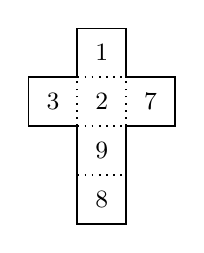
\begin{tikzpicture}[scale=0.62, line width=0.5pt]
  % 바깥 테두리
  \draw[line width=0.6pt] (1,4) -- (2,4) -- (2,3) -- (3,3) -- (3,2) -- (2,2) -- (2,0) -- (1,0) -- (1,2) -- (0,2) -- (0,3) -- (1,3) -- cycle;
  % 접는 선(원문의 점선)
  \draw[dotted, line width=0.6pt] (1,3) -- (2,3);
  \draw[dotted, line width=0.6pt] (1,2) -- (2,2);
  \draw[dotted, line width=0.6pt] (1,1) -- (2,1);
  \draw[dotted, line width=0.6pt] (1,2) -- (1,3);
  \draw[dotted, line width=0.6pt] (2,2) -- (2,3);
  \node[font=\small] at (1.5,3.5) {$1$};
  \node[font=\small] at (0.5,2.5) {$3$};
  \node[font=\small] at (1.5,2.5) {$2$};
  \node[font=\small] at (2.5,2.5) {$7$};
  \node[font=\small] at (1.5,1.5) {$9$};
  \node[font=\small] at (1.5,0.5) {$8$};
\end{tikzpicture}
}\end{minipage}\par
\par\medskip\par\noindent\hangindent=1.4em\hangafter=1 {\small ①}\ $A=\{2{,}\mkern3mu\mathopen{}8\}$\par\noindent\hangindent=1.4em\hangafter=1 {\small ②}\ $B=\{3{,}\mkern3mu\mathopen{}9\}$\par\noindent\hangindent=1.4em\hangafter=1 {\small ③}\ $A\not\subset \comp{B}$\par\noindent\hangindent=1.4em\hangafter=1 {\small ④}\ 두 사건 $A$와 $B$는 서로 배반사건이다.\par\noindent\hangindent=1.4em\hangafter=1 {\small ⑤}\ 이 시행의 근원사건은 $\{1\}$, $\{2\}$, $\{3\}$, $\{7\}$, $\{8\}$, $\{9\}$이다.\par\medskip
}\vspace{8mm}
\setcounter{dmproblemcount}{7}\dmpnum{41-08}{% id: 41-08
% book: 베이직쎈 확률과 통계 · 03 확률의 뜻과 활용
% section: 유형 023 배반사건
% figure: none
% answer: 
% answer_source: 
% variant_level: 0 (원본 전사)
% 이 파일은 build.mjs 가 items.json 에서 만든다. 고칠 때는 items.json 을 고친다.
\smash{\raisebox{1.5mm}{\dmkichul{베이직쎈 확률과 통계 41쪽 08번}}}
1부터 20까지의 자연수가 각각 하나씩 적힌 20장의 카드 중 임의로 한 장의 카드를 뽑는 시행에서 세 사건 $A$, $B$, $C$가 각각 다음과 같을 때, 서로 배반사건인 것만을 보기에서 있는 대로 고른 것은?\exprbox{\begin{minipage}{0.96\linewidth}\raggedright $A$: 5의 배수가 적힌 카드를 뽑는 사건\\ $B$: 9의 배수가 적힌 카드를 뽑는 사건\\ $C$: 15의 약수가 적힌 카드를 뽑는 사건\end{minipage}}\bogi{ㄱ. $A$와 $B$ \hfill ㄴ. $A$와 $C$ \hfill ㄷ. $B$와 $C$}
\dmchoicesauto{}{ㄱ}{ㄷ}{ㄱ, ㄴ}{ㄱ, ㄷ}{ㄴ, ㄷ}
}\vspace{8mm}
\setcounter{dmproblemcount}{8}\dmpnum{41-09}{% id: 41-09
% book: 베이직쎈 확률과 통계 · 03 확률의 뜻과 활용
% section: 유형 023 배반사건
% figure: tikz:fig-41-09
% answer: 
% answer_source: 
% variant_level: 0 (원본 전사)
% 이 파일은 build.mjs 가 items.json 에서 만든다. 고칠 때는 items.json 을 고친다.
\smash{\raisebox{1.5mm}{\dmkichul{베이직쎈 확률과 통계 41쪽 09번}}}
\noindent\begin{minipage}[t]{0.58\linewidth}\vspace{0pt}\raggedright 표본공간 $S=\{1{,}\mkern3mu\mathopen{}2{,}\mkern3mu\mathopen{}3{,}\mkern3mu\mathopen{}4{,}\mkern3mu\mathopen{}5{,}\mkern3mu\mathopen{}6\}$의 부분집합인 두 사건 $A$, $B$가 오른쪽 벤 다이어그램과 같을 때, 옳은 것만을 보기에서 있는 대로 고르시오.\end{minipage}\hfill\begin{minipage}[t]{0.4\linewidth}\vspace{0pt}\centering \resizebox{\ifdim\width>\linewidth\linewidth\else\width\fi}{!}{% 유형 023 41-09(인쇄 41쪽) — 표본공간 S 안에 사건 A 의 원, 그 안에 사건 B 의 원이 놓인 벤 다이어그램.
%   원소 자리: A 밖 1·4, A 안 B 밖 2·5, B 안 3·6. 스캔 화질이 낮아 TikZ 로 다시 그림.
% 라벨(S·A·B·원소)은 원문에 있는 것만. 라벨은 원문처럼 선을 끊고 그 자리에 놓는다.
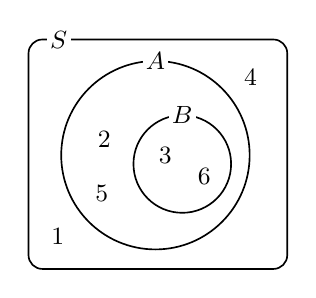
\begin{tikzpicture}[scale=0.62, line width=0.5pt]
  \draw[rounded corners=5pt, line width=0.6pt] (0,0) rectangle (5.3,4.7);
  \draw[line width=0.6pt] (2.6,2.33) circle (1.93);
  \draw[line width=0.6pt] (3.15,2.15) circle (1.0);
  \node[fill=white, inner sep=1.2pt, font=\small] at (0.62,4.7) {$S$};
  \node[fill=white, inner sep=1.2pt, font=\small] at (2.6,4.26) {$A$};
  \node[fill=white, inner sep=1.2pt, font=\small] at (3.15,3.15) {$B$};
  \node[font=\small] at (1.55,2.65) {$2$};
  \node[font=\small] at (1.50,1.55) {$5$};
  \node[font=\small] at (2.80,2.32) {$3$};
  \node[font=\small] at (3.60,1.90) {$6$};
  \node[font=\small] at (0.60,0.67) {$1$};
  \node[font=\small] at (4.55,3.92) {$4$};
\end{tikzpicture}
}\end{minipage}\par
\noindent \bogi{ㄱ. $A$와 $\comp{B}$는 서로 배반사건이 아니다.\\ ㄴ. $\comp{A}$와 $B$는 서로 배반사건이다.\\ ㄷ. $\comp{A}$와 $\comp{B}$는 서로 배반사건이다.}
}\vspace{8mm}
\setcounter{dmproblemcount}{9}\dmpnum{41-10}{% id: 41-10
% book: 베이직쎈 확률과 통계 · 03 확률의 뜻과 활용
% section: 유형 023 배반사건
% figure: none
% answer: 
% answer_source: 
% variant_level: 0 (원본 전사)
% 이 파일은 build.mjs 가 items.json 에서 만든다. 고칠 때는 items.json 을 고친다.
\smash{\raisebox{1.5mm}{\dmkichul{베이직쎈 확률과 통계 41쪽 10번}}}
표본공간 $S$의 두 사건 $A$, $B$가 서로 배반사건일 때, 다음 중 항상 옳은 것이 \underline{아닌} 것은?
\begin{choicesii}{$A\cap B=\varnothing$}{$\comp{A}\cap B=B$}{$A\cup B=S$}{$A\subset \comp{B}$}{$B\subset \comp{A}$}\end{choicesii}
}\vspace{8mm}
\setcounter{dmproblemcount}{10}\dmpnum{41-11}{% id: 41-11
% book: 베이직쎈 확률과 통계 · 03 확률의 뜻과 활용
% section: 유형 023 배반사건
% figure: none
% answer: 
% answer_source: 
% variant_level: 0 (원본 전사)
% 이 파일은 build.mjs 가 items.json 에서 만든다. 고칠 때는 items.json 을 고친다.
\smash{\raisebox{1.5mm}{\dmkichul{베이직쎈 확률과 통계 41쪽 11번}}}
표본공간 $S=\{x \mid x$는 10 미만의 자연수$\}$의 두 사건 $A$, $B$가\par\smallskip\dispeq{$A=\{x \mid x$는 8의 약수$\}$, $B=\{x \mid x$는 소수$\}$}\par\smallskip\noindent 일 때, 표본공간 $S$의 사건 중에서 두 사건 $A$, $B$와 모두 배반인 사건 $C$를 모두 구하시오.
}\vspace{8mm}
\dmsection{개념 12 수학적 확률}
\setcounter{dmproblemcount}{0}\dmpnum{42-01}{% id: 42-01
% book: 베이직쎈 확률과 통계 · 03 확률의 뜻과 활용
% section: 개념 12 수학적 확률
% figure: none
% answer: 
% answer_source: 
% variant_level: 0 (원본 전사)
% 이 파일은 build.mjs 가 items.json 에서 만든다. 고칠 때는 items.json 을 고친다.
\smash{\raisebox{1.5mm}{\dmkichul{베이직쎈 확률과 통계 42쪽 01번}}}
한 개의 주사위를 던지는 시행에서 표본공간을 $S$, 3의 배수의 눈이 나오는 사건을 $A$라 할 때, 다음을 구하시오.
\dmsubprob{1} $n(S)$
\dmsubprob{2} $n(A)$
\dmsubprob{3} $\mathrm{P}(A)$
}\vspace{8mm}
\dmpassage{노란 공 3개, 검은 공 5개가 들어 있는 주머니에서 임의로 한 개의 공을 꺼낼 때, 노란 공을 꺼내는 사건을 $A$, 검은 공을 꺼내는 사건을 $B$라 하자. 다음을 구하시오.}
\setcounter{dmproblemcount}{1}\dmpnum{42-02}{% id: 42-02
% book: 베이직쎈 확률과 통계 · 03 확률의 뜻과 활용
% section: 개념 12 수학적 확률
% passage: 노란 공 3개, 검은 공 5개가 들어 있는 주머니에서 임의로 한 개의 공을 꺼낼 때, 노란 공을 꺼내는 사건을 $A$, 검은 공을 꺼내는 사건을 $B$라 하자. 다음을 구하시오.
% figure: none
% answer: 
% answer_source: 
% variant_level: 0 (원본 전사)
% 이 파일은 build.mjs 가 items.json 에서 만든다. 고칠 때는 items.json 을 고친다.
\smash{\raisebox{1.5mm}{\dmkichul{베이직쎈 확률과 통계 42쪽 02번}}}
$\mathrm{P}(A)$
}\vspace{8mm}
\setcounter{dmproblemcount}{2}\dmpnum{42-03}{% id: 42-03
% book: 베이직쎈 확률과 통계 · 03 확률의 뜻과 활용
% section: 개념 12 수학적 확률
% passage: 노란 공 3개, 검은 공 5개가 들어 있는 주머니에서 임의로 한 개의 공을 꺼낼 때, 노란 공을 꺼내는 사건을 $A$, 검은 공을 꺼내는 사건을 $B$라 하자. 다음을 구하시오.
% figure: none
% answer: 
% answer_source: 
% variant_level: 0 (원본 전사)
% 이 파일은 build.mjs 가 items.json 에서 만든다. 고칠 때는 items.json 을 고친다.
\smash{\raisebox{1.5mm}{\dmkichul{베이직쎈 확률과 통계 42쪽 03번}}}
$\mathrm{P}(B)$
}\vspace{8mm}
\dmpassage{서로 다른 두 개의 동전을 동시에 던질 때, 다음을 구하시오.}
\setcounter{dmproblemcount}{3}\dmpnum{42-04}{% id: 42-04
% book: 베이직쎈 확률과 통계 · 03 확률의 뜻과 활용
% section: 개념 12 수학적 확률
% passage: 서로 다른 두 개의 동전을 동시에 던질 때, 다음을 구하시오.
% figure: none
% answer: 
% answer_source: 
% variant_level: 0 (원본 전사)
% 이 파일은 build.mjs 가 items.json 에서 만든다. 고칠 때는 items.json 을 고친다.
\smash{\raisebox{1.5mm}{\dmkichul{베이직쎈 확률과 통계 42쪽 04번}}}
두 개 모두 뒷면이 나올 확률
}\vspace{8mm}
\setcounter{dmproblemcount}{4}\dmpnum{42-05}{% id: 42-05
% book: 베이직쎈 확률과 통계 · 03 확률의 뜻과 활용
% section: 개념 12 수학적 확률
% passage: 서로 다른 두 개의 동전을 동시에 던질 때, 다음을 구하시오.
% figure: none
% answer: 
% answer_source: 
% variant_level: 0 (원본 전사)
% 이 파일은 build.mjs 가 items.json 에서 만든다. 고칠 때는 items.json 을 고친다.
\smash{\raisebox{1.5mm}{\dmkichul{베이직쎈 확률과 통계 42쪽 05번}}}
서로 다른 면이 나올 확률
}\vspace{8mm}
\setcounter{dmproblemcount}{5}\dmpnum{42-06}{% id: 42-06
% book: 베이직쎈 확률과 통계 · 03 확률의 뜻과 활용
% section: 개념 12 수학적 확률
% passage: 서로 다른 두 개의 동전을 동시에 던질 때, 다음을 구하시오.
% figure: none
% answer: 
% answer_source: 
% variant_level: 0 (원본 전사)
% 이 파일은 build.mjs 가 items.json 에서 만든다. 고칠 때는 items.json 을 고친다.
\smash{\raisebox{1.5mm}{\dmkichul{베이직쎈 확률과 통계 42쪽 06번}}}
적어도 한 개는 앞면이 나올 확률
}\vspace{8mm}
\dmpassage{서로 다른 두 개의 주사위를 동시에 던질 때, 다음을 구하시오.}
\setcounter{dmproblemcount}{6}\dmpnum{42-07}{% id: 42-07
% book: 베이직쎈 확률과 통계 · 03 확률의 뜻과 활용
% section: 개념 12 수학적 확률
% passage: 서로 다른 두 개의 주사위를 동시에 던질 때, 다음을 구하시오.
% figure: none
% answer: 
% answer_source: 
% variant_level: 0 (원본 전사)
% 이 파일은 build.mjs 가 items.json 에서 만든다. 고칠 때는 items.json 을 고친다.
\smash{\raisebox{1.5mm}{\dmkichul{베이직쎈 확률과 통계 42쪽 07번}}}
나온 두 눈의 수가 서로 같을 확률
}\vspace{8mm}
\setcounter{dmproblemcount}{7}\dmpnum{42-08}{% id: 42-08
% book: 베이직쎈 확률과 통계 · 03 확률의 뜻과 활용
% section: 개념 12 수학적 확률
% passage: 서로 다른 두 개의 주사위를 동시에 던질 때, 다음을 구하시오.
% figure: none
% answer: 
% answer_source: 
% variant_level: 0 (원본 전사)
% 이 파일은 build.mjs 가 items.json 에서 만든다. 고칠 때는 items.json 을 고친다.
\smash{\raisebox{1.5mm}{\dmkichul{베이직쎈 확률과 통계 42쪽 08번}}}
나온 두 눈의 수의 합이 5일 확률
}\vspace{8mm}
\setcounter{dmproblemcount}{8}\dmpnum{43-09}{% id: 43-09
% book: 베이직쎈 확률과 통계 · 03 확률의 뜻과 활용
% section: 개념 12 수학적 확률
% passage: 서로 다른 두 개의 주사위를 동시에 던질 때, 다음을 구하시오.
% figure: none
% answer: 
% answer_source: 
% variant_level: 0 (원본 전사)
% 이 파일은 build.mjs 가 items.json 에서 만든다. 고칠 때는 items.json 을 고친다.
\smash{\raisebox{1.5mm}{\dmkichul{베이직쎈 확률과 통계 43쪽 09번}}}
나온 두 눈의 수의 차가 3일 확률
}\vspace{8mm}
\setcounter{dmproblemcount}{9}\dmpnum{43-10}{% id: 43-10
% book: 베이직쎈 확률과 통계 · 03 확률의 뜻과 활용
% section: 개념 12 수학적 확률
% passage: 서로 다른 두 개의 주사위를 동시에 던질 때, 다음을 구하시오.
% figure: none
% answer: 
% answer_source: 
% variant_level: 0 (원본 전사)
% 이 파일은 build.mjs 가 items.json 에서 만든다. 고칠 때는 items.json 을 고친다.
\smash{\raisebox{1.5mm}{\dmkichul{베이직쎈 확률과 통계 43쪽 10번}}}
나온 두 눈의 수의 곱이 4일 확률
}\vspace{8mm}
\setcounter{dmproblemcount}{10}\dmpnum{43-11}{% id: 43-11
% book: 베이직쎈 확률과 통계 · 03 확률의 뜻과 활용
% section: 개념 12 수학적 확률
% figure: none
% answer: 
% answer_source: 
% variant_level: 0 (원본 전사)
% 이 파일은 build.mjs 가 items.json 에서 만든다. 고칠 때는 items.json 을 고친다.
\smash{\raisebox{1.5mm}{\dmkichul{베이직쎈 확률과 통계 43쪽 11번}}}
4개의 문자 $\pt{A}$, $\pt{B}$, $\pt{C}$, $\pt{D}$를 일렬로 나열할 때, 다음을 구하시오.
\dmsubprob{1} 모든 경우의 수
\dmsubprob{2} $\pt{A}$가 맨 앞에 오도록 나열하는 경우의 수
\dmsubprob{3} $\pt{A}$가 맨 앞에 올 확률
}\vspace{8mm}
\dmpassage{5명의 학생 $\pt{A}$, $\pt{B}$, $\pt{C}$, $\pt{D}$, $\pt{E}$가 일렬로 설 때, 다음을 구하시오.}
\setcounter{dmproblemcount}{11}\dmpnum{43-12}{% id: 43-12
% book: 베이직쎈 확률과 통계 · 03 확률의 뜻과 활용
% section: 개념 12 수학적 확률
% passage: 5명의 학생 $\pt{A}$, $\pt{B}$, $\pt{C}$, $\pt{D}$, $\pt{E}$가 일렬로 설 때, 다음을 구하시오.
% figure: none
% answer: 
% answer_source: 
% variant_level: 0 (원본 전사)
% 이 파일은 build.mjs 가 items.json 에서 만든다. 고칠 때는 items.json 을 고친다.
\smash{\raisebox{1.5mm}{\dmkichul{베이직쎈 확률과 통계 43쪽 12번}}}
$\pt{A}$가 맨 뒤에 설 확률
}\vspace{8mm}
\setcounter{dmproblemcount}{12}\dmpnum{43-13}{% id: 43-13
% book: 베이직쎈 확률과 통계 · 03 확률의 뜻과 활용
% section: 개념 12 수학적 확률
% passage: 5명의 학생 $\pt{A}$, $\pt{B}$, $\pt{C}$, $\pt{D}$, $\pt{E}$가 일렬로 설 때, 다음을 구하시오.
% figure: none
% answer: 
% answer_source: 
% variant_level: 0 (원본 전사)
% 이 파일은 build.mjs 가 items.json 에서 만든다. 고칠 때는 items.json 을 고친다.
\smash{\raisebox{1.5mm}{\dmkichul{베이직쎈 확률과 통계 43쪽 13번}}}
$\pt{A}$와 $\pt{B}$가 이웃하게 설 확률
}\vspace{8mm}
\setcounter{dmproblemcount}{13}\dmpnum{43-14}{% id: 43-14
% book: 베이직쎈 확률과 통계 · 03 확률의 뜻과 활용
% section: 개념 12 수학적 확률
% passage: 5명의 학생 $\pt{A}$, $\pt{B}$, $\pt{C}$, $\pt{D}$, $\pt{E}$가 일렬로 설 때, 다음을 구하시오.
% figure: none
% answer: 
% answer_source: 
% variant_level: 0 (원본 전사)
% 이 파일은 build.mjs 가 items.json 에서 만든다. 고칠 때는 items.json 을 고친다.
\smash{\raisebox{1.5mm}{\dmkichul{베이직쎈 확률과 통계 43쪽 14번}}}
$\pt{A}$와 $\pt{B}$가 이웃하지 않게 설 확률
}\vspace{8mm}
\setcounter{dmproblemcount}{14}\dmpnum{43-15}{% id: 43-15
% book: 베이직쎈 확률과 통계 · 03 확률의 뜻과 활용
% section: 개념 12 수학적 확률
% passage: 5명의 학생 $\pt{A}$, $\pt{B}$, $\pt{C}$, $\pt{D}$, $\pt{E}$가 일렬로 설 때, 다음을 구하시오.
% figure: none
% answer: 
% answer_source: 
% variant_level: 0 (원본 전사)
% 이 파일은 build.mjs 가 items.json 에서 만든다. 고칠 때는 items.json 을 고친다.
\smash{\raisebox{1.5mm}{\dmkichul{베이직쎈 확률과 통계 43쪽 15번}}}
$\pt{A}$의 양옆에 $\pt{B}$, $\pt{C}$가 설 확률
}\vspace{8mm}
\setcounter{dmproblemcount}{15}\dmpnum{43-16}{% id: 43-16
% book: 베이직쎈 확률과 통계 · 03 확률의 뜻과 활용
% section: 개념 12 수학적 확률
% figure: none
% answer: 
% answer_source: 
% variant_level: 0 (원본 전사)
% 이 파일은 build.mjs 가 items.json 에서 만든다. 고칠 때는 items.json 을 고친다.
\smash{\raisebox{1.5mm}{\dmkichul{베이직쎈 확률과 통계 43쪽 16번}}}
빨간 구슬 3개, 파란 구슬 2개가 들어 있는 주머니에서 임의로 2개의 구슬을 동시에 꺼낼 때, 다음을 구하시오.
\dmsubprob{1} 모든 경우의 수
\dmsubprob{2} 2개 모두 빨간 구슬을 꺼내는 경우의 수
\dmsubprob{3} 2개 모두 빨간 구슬을 꺼낼 확률
}\vspace{8mm}
\dmpassage{흰 공 4개, 파란 공 2개가 들어 있는 주머니에서 임의로 2개의 공을 동시에 꺼낼 때, 다음을 구하시오.}
\setcounter{dmproblemcount}{16}\dmpnum{43-17}{% id: 43-17
% book: 베이직쎈 확률과 통계 · 03 확률의 뜻과 활용
% section: 개념 12 수학적 확률
% passage: 흰 공 4개, 파란 공 2개가 들어 있는 주머니에서 임의로 2개의 공을 동시에 꺼낼 때, 다음을 구하시오.
% figure: none
% answer: 
% answer_source: 
% variant_level: 0 (원본 전사)
% 이 파일은 build.mjs 가 items.json 에서 만든다. 고칠 때는 items.json 을 고친다.
\smash{\raisebox{1.5mm}{\dmkichul{베이직쎈 확률과 통계 43쪽 17번}}}
2개 모두 흰 공을 꺼낼 확률
}\vspace{8mm}
\setcounter{dmproblemcount}{17}\dmpnum{43-18}{% id: 43-18
% book: 베이직쎈 확률과 통계 · 03 확률의 뜻과 활용
% section: 개념 12 수학적 확률
% passage: 흰 공 4개, 파란 공 2개가 들어 있는 주머니에서 임의로 2개의 공을 동시에 꺼낼 때, 다음을 구하시오.
% figure: none
% answer: 
% answer_source: 
% variant_level: 0 (원본 전사)
% 이 파일은 build.mjs 가 items.json 에서 만든다. 고칠 때는 items.json 을 고친다.
\smash{\raisebox{1.5mm}{\dmkichul{베이직쎈 확률과 통계 43쪽 18번}}}
흰 공 1개, 파란 공 1개를 꺼낼 확률
}\vspace{8mm}
\dmsection{개념 13 통계적 확률}
\dmpassage{다음에 답하시오.}
\setcounter{dmproblemcount}{18}\dmpnum{44-19}{% id: 44-19
% book: 베이직쎈 확률과 통계 · 03 확률의 뜻과 활용
% section: 개념 13 통계적 확률
% passage: 다음에 답하시오.
% figure: none
% answer: 
% answer_source: 
% variant_level: 0 (원본 전사)
% 이 파일은 build.mjs 가 items.json 에서 만든다. 고칠 때는 items.json 을 고친다.
\smash{\raisebox{1.5mm}{\dmkichul{베이직쎈 확률과 통계 44쪽 19번}}}
한 개의 윷짝을 800번 던졌을 때, 평평한 면이 480번 나왔다. 이 윷짝을 한 번 던질 때, 평평한 면이 나올 확률을 구하시오.
}\vspace{8mm}
\setcounter{dmproblemcount}{19}\dmpnum{44-20}{% id: 44-20
% book: 베이직쎈 확률과 통계 · 03 확률의 뜻과 활용
% section: 개념 13 통계적 확률
% passage: 다음에 답하시오.
% figure: none
% answer: 
% answer_source: 
% variant_level: 0 (원본 전사)
% 이 파일은 build.mjs 가 items.json 에서 만든다. 고칠 때는 items.json 을 고친다.
\smash{\raisebox{1.5mm}{\dmkichul{베이직쎈 확률과 통계 44쪽 20번}}}
한 개의 압정을 400번 던졌을 때, 평평한 면이 바닥에 220번 닿았다. 이 압정을 한 번 던질 때, 평평한 면이 바닥에 닿을 확률을 구하시오.
}\vspace{8mm}
\setcounter{dmproblemcount}{20}\dmpnum{44-21}{% id: 44-21
% book: 베이직쎈 확률과 통계 · 03 확률의 뜻과 활용
% section: 개념 13 통계적 확률
% passage: 다음에 답하시오.
% figure: none
% answer: 
% answer_source: 
% variant_level: 0 (원본 전사)
% 이 파일은 build.mjs 가 items.json 에서 만든다. 고칠 때는 items.json 을 고친다.
\smash{\raisebox{1.5mm}{\dmkichul{베이직쎈 확률과 통계 44쪽 21번}}}
어느 야구 선수가 250개의 공을 쳤을 때, 80개의 안타를 쳤다. 이 선수가 한 개의 공을 칠 때, 안타를 칠 확률을 구하시오.
}\vspace{8mm}
\dmpassage{아래는 어느 지역의 휴대폰 사용자 400명을 대상으로 이용하는 통신사를 조사하여 나타낸 표이다. 이 사용자 중에서 임의로 한 명을 택할 때, 다음을 구하시오.}
\begin{center}\resizebox{\ifdim\width>\linewidth\linewidth\else\width\fi}{!}{% 개념 13 44-22~23(인쇄 44쪽) — 공통 지시문의 통신사별 사용자 수 표. 스캔 표라 tabular 로 다시 조판(칸 값 원문 그대로).
{\setlength{\tabcolsep}{6pt}\renewcommand{\arraystretch}{1.3}%
\begin{tabular}{|c|c|c|c|c|}
\hline
\textbf{통신사} & \makebox[11mm]{$\mathrm{A}$} & \makebox[11mm]{$\mathrm{B}$} & \makebox[11mm]{$\mathrm{C}$} & \textbf{합계} \\
\hline
\textbf{사용자 수} & $210$ & $80$ & $110$ & $400$ \\
\hline
\end{tabular}}
}\end{center}\vspace{4mm}
\setcounter{dmproblemcount}{21}\dmpnum{44-22}{% id: 44-22
% book: 베이직쎈 확률과 통계 · 03 확률의 뜻과 활용
% section: 개념 13 통계적 확률
% passage: 아래는 어느 지역의 휴대폰 사용자 400명을 대상으로 이용하는 통신사를 조사하여 나타낸 표이다. 이 사용자 중에서 임의로 한 명을 택할 때, 다음을 구하시오.
% figure: tikz:fig-44-22
% answer: 
% answer_source: 
% variant_level: 0 (원본 전사)
% 이 파일은 build.mjs 가 items.json 에서 만든다. 고칠 때는 items.json 을 고친다.
\smash{\raisebox{1.5mm}{\dmkichul{베이직쎈 확률과 통계 44쪽 22번}}}
택한 사람이 $\mathrm{A}$ 통신사를 이용할 확률
}\vspace{8mm}
\setcounter{dmproblemcount}{22}\dmpnum{44-23}{% id: 44-23
% book: 베이직쎈 확률과 통계 · 03 확률의 뜻과 활용
% section: 개념 13 통계적 확률
% passage: 아래는 어느 지역의 휴대폰 사용자 400명을 대상으로 이용하는 통신사를 조사하여 나타낸 표이다. 이 사용자 중에서 임의로 한 명을 택할 때, 다음을 구하시오.
% figure: tikz:fig-44-22
% answer: 
% answer_source: 
% variant_level: 0 (원본 전사)
% 이 파일은 build.mjs 가 items.json 에서 만든다. 고칠 때는 items.json 을 고친다.
\smash{\raisebox{1.5mm}{\dmkichul{베이직쎈 확률과 통계 44쪽 23번}}}
택한 사람이 $\mathrm{B}$ 통신사를 이용할 확률
}\vspace{8mm}
\dmpassage{아래는 어느 학교의 학생 500명의 혈액형을 조사하여 나타낸 표이다. 이 학교 학생 중에서 임의로 한 명을 택할 때, 다음을 구하시오.}
\begin{center}\resizebox{\ifdim\width>\linewidth\linewidth\else\width\fi}{!}{% 개념 13 44-24~25(인쇄 44쪽) — 공통 지시문의 혈액형별 학생 수 표. 스캔 표라 tabular 로 다시 조판(칸 값 원문 그대로).
{\setlength{\tabcolsep}{6pt}\renewcommand{\arraystretch}{1.3}%
\begin{tabular}{|c|c|c|c|c|c|}
\hline
\textbf{혈액형} & \makebox[10mm]{$\mathrm{A}$형} & \makebox[10mm]{$\mathrm{B}$형} & \makebox[10mm]{$\mathrm{O}$형} & \makebox[12mm]{$\mathrm{AB}$형} & \textbf{합계} \\
\hline
\textbf{학생 수} & $130$ & $120$ & $150$ & $100$ & $500$ \\
\hline
\end{tabular}}
}\end{center}\vspace{4mm}
\setcounter{dmproblemcount}{23}\dmpnum{44-24}{% id: 44-24
% book: 베이직쎈 확률과 통계 · 03 확률의 뜻과 활용
% section: 개념 13 통계적 확률
% passage: 아래는 어느 학교의 학생 500명의 혈액형을 조사하여 나타낸 표이다. 이 학교 학생 중에서 임의로 한 명을 택할 때, 다음을 구하시오.
% figure: tikz:fig-44-24
% answer: 
% answer_source: 
% variant_level: 0 (원본 전사)
% 이 파일은 build.mjs 가 items.json 에서 만든다. 고칠 때는 items.json 을 고친다.
\smash{\raisebox{1.5mm}{\dmkichul{베이직쎈 확률과 통계 44쪽 24번}}}
택한 학생의 혈액형이 $\mathrm{B}$형일 확률
}\vspace{8mm}
\setcounter{dmproblemcount}{24}\dmpnum{44-25}{% id: 44-25
% book: 베이직쎈 확률과 통계 · 03 확률의 뜻과 활용
% section: 개념 13 통계적 확률
% passage: 아래는 어느 학교의 학생 500명의 혈액형을 조사하여 나타낸 표이다. 이 학교 학생 중에서 임의로 한 명을 택할 때, 다음을 구하시오.
% figure: tikz:fig-44-24
% answer: 
% answer_source: 
% variant_level: 0 (원본 전사)
% 이 파일은 build.mjs 가 items.json 에서 만든다. 고칠 때는 items.json 을 고친다.
\smash{\raisebox{1.5mm}{\dmkichul{베이직쎈 확률과 통계 44쪽 25번}}}
택한 학생의 혈액형이 $\mathrm{O}$형일 확률
}\vspace{8mm}
\dmsection{개념 14 확률의 기본 성질}
\dmpassage{한 개의 주사위를 던질 때, 다음을 구하시오.}
\setcounter{dmproblemcount}{25}\dmpnum{45-26}{% id: 45-26
% book: 베이직쎈 확률과 통계 · 03 확률의 뜻과 활용
% section: 개념 14 확률의 기본 성질
% passage: 한 개의 주사위를 던질 때, 다음을 구하시오.
% figure: none
% answer: 
% answer_source: 
% variant_level: 0 (원본 전사)
% 이 파일은 build.mjs 가 items.json 에서 만든다. 고칠 때는 items.json 을 고친다.
\smash{\raisebox{1.5mm}{\dmkichul{베이직쎈 확률과 통계 45쪽 26번}}}
소수의 눈이 나올 확률
}\vspace{8mm}
\setcounter{dmproblemcount}{26}\dmpnum{45-27}{% id: 45-27
% book: 베이직쎈 확률과 통계 · 03 확률의 뜻과 활용
% section: 개념 14 확률의 기본 성질
% passage: 한 개의 주사위를 던질 때, 다음을 구하시오.
% figure: none
% answer: 
% answer_source: 
% variant_level: 0 (원본 전사)
% 이 파일은 build.mjs 가 items.json 에서 만든다. 고칠 때는 items.json 을 고친다.
\smash{\raisebox{1.5mm}{\dmkichul{베이직쎈 확률과 통계 45쪽 27번}}}
자연수의 눈이 나올 확률
}\vspace{8mm}
\setcounter{dmproblemcount}{27}\dmpnum{45-28}{% id: 45-28
% book: 베이직쎈 확률과 통계 · 03 확률의 뜻과 활용
% section: 개념 14 확률의 기본 성질
% passage: 한 개의 주사위를 던질 때, 다음을 구하시오.
% figure: none
% answer: 
% answer_source: 
% variant_level: 0 (원본 전사)
% 이 파일은 build.mjs 가 items.json 에서 만든다. 고칠 때는 items.json 을 고친다.
\smash{\raisebox{1.5mm}{\dmkichul{베이직쎈 확률과 통계 45쪽 28번}}}
$0$의 눈이 나올 확률
}\vspace{8mm}
\dmpassage{흰 구슬 2개, 검은 구슬 3개가 들어 있는 주머니에서 임의로 한 개의 구슬을 꺼낼 때, 다음을 구하시오.}
\setcounter{dmproblemcount}{28}\dmpnum{45-29}{% id: 45-29
% book: 베이직쎈 확률과 통계 · 03 확률의 뜻과 활용
% section: 개념 14 확률의 기본 성질
% passage: 흰 구슬 2개, 검은 구슬 3개가 들어 있는 주머니에서 임의로 한 개의 구슬을 꺼낼 때, 다음을 구하시오.
% figure: none
% answer: 
% answer_source: 
% variant_level: 0 (원본 전사)
% 이 파일은 build.mjs 가 items.json 에서 만든다. 고칠 때는 items.json 을 고친다.
\smash{\raisebox{1.5mm}{\dmkichul{베이직쎈 확률과 통계 45쪽 29번}}}
검은 구슬을 꺼낼 확률
}\vspace{8mm}
\setcounter{dmproblemcount}{29}\dmpnum{45-30}{% id: 45-30
% book: 베이직쎈 확률과 통계 · 03 확률의 뜻과 활용
% section: 개념 14 확률의 기본 성질
% passage: 흰 구슬 2개, 검은 구슬 3개가 들어 있는 주머니에서 임의로 한 개의 구슬을 꺼낼 때, 다음을 구하시오.
% figure: none
% answer: 
% answer_source: 
% variant_level: 0 (원본 전사)
% 이 파일은 build.mjs 가 items.json 에서 만든다. 고칠 때는 items.json 을 고친다.
\smash{\raisebox{1.5mm}{\dmkichul{베이직쎈 확률과 통계 45쪽 30번}}}
흰 구슬 또는 검은 구슬을 꺼낼 확률
}\vspace{8mm}
\setcounter{dmproblemcount}{30}\dmpnum{45-31}{% id: 45-31
% book: 베이직쎈 확률과 통계 · 03 확률의 뜻과 활용
% section: 개념 14 확률의 기본 성질
% passage: 흰 구슬 2개, 검은 구슬 3개가 들어 있는 주머니에서 임의로 한 개의 구슬을 꺼낼 때, 다음을 구하시오.
% figure: none
% answer: 
% answer_source: 
% variant_level: 0 (원본 전사)
% 이 파일은 build.mjs 가 items.json 에서 만든다. 고칠 때는 items.json 을 고친다.
\smash{\raisebox{1.5mm}{\dmkichul{베이직쎈 확률과 통계 45쪽 31번}}}
노란 구슬을 꺼낼 확률
}\vspace{8mm}
\dmpassage{$1$부터 $7$까지의 자연수가 각각 하나씩 적힌 7개의 공이 들어 있는 상자에서 임의로 한 개의 공을 꺼낼 때, 다음을 구하시오.}
\setcounter{dmproblemcount}{31}\dmpnum{45-32}{% id: 45-32
% book: 베이직쎈 확률과 통계 · 03 확률의 뜻과 활용
% section: 개념 14 확률의 기본 성질
% passage: $1$부터 $7$까지의 자연수가 각각 하나씩 적힌 7개의 공이 들어 있는 상자에서 임의로 한 개의 공을 꺼낼 때, 다음을 구하시오.
% figure: none
% answer: 
% answer_source: 
% variant_level: 0 (원본 전사)
% 이 파일은 build.mjs 가 items.json 에서 만든다. 고칠 때는 items.json 을 고친다.
\smash{\raisebox{1.5mm}{\dmkichul{베이직쎈 확률과 통계 45쪽 32번}}}
$6$의 약수가 적힌 공을 꺼낼 확률
}\vspace{8mm}
\setcounter{dmproblemcount}{32}\dmpnum{45-33}{% id: 45-33
% book: 베이직쎈 확률과 통계 · 03 확률의 뜻과 활용
% section: 개념 14 확률의 기본 성질
% passage: $1$부터 $7$까지의 자연수가 각각 하나씩 적힌 7개의 공이 들어 있는 상자에서 임의로 한 개의 공을 꺼낼 때, 다음을 구하시오.
% figure: none
% answer: 
% answer_source: 
% variant_level: 0 (원본 전사)
% 이 파일은 build.mjs 가 items.json 에서 만든다. 고칠 때는 items.json 을 고친다.
\smash{\raisebox{1.5mm}{\dmkichul{베이직쎈 확률과 통계 45쪽 33번}}}
$7$ 이하의 자연수가 적힌 공을 꺼낼 확률
}\vspace{8mm}
\setcounter{dmproblemcount}{33}\dmpnum{45-34}{% id: 45-34
% book: 베이직쎈 확률과 통계 · 03 확률의 뜻과 활용
% section: 개념 14 확률의 기본 성질
% passage: $1$부터 $7$까지의 자연수가 각각 하나씩 적힌 7개의 공이 들어 있는 상자에서 임의로 한 개의 공을 꺼낼 때, 다음을 구하시오.
% figure: none
% answer: 
% answer_source: 
% variant_level: 0 (원본 전사)
% 이 파일은 build.mjs 가 items.json 에서 만든다. 고칠 때는 items.json 을 고친다.
\smash{\raisebox{1.5mm}{\dmkichul{베이직쎈 확률과 통계 45쪽 34번}}}
$8$이 적힌 공을 꺼낼 확률
}\vspace{8mm}
\dmpassage{$1$부터 $10$까지의 자연수가 각각 하나씩 적힌 10장의 카드 중에서 임의로 한 장의 카드를 뽑을 때, 짝수가 적힌 카드를 뽑는 사건을 $A$, 홀수가 적힌 카드를 뽑는 사건을 $B$라 하자. 다음을 구하시오.}
\setcounter{dmproblemcount}{34}\dmpnum{45-35}{% id: 45-35
% book: 베이직쎈 확률과 통계 · 03 확률의 뜻과 활용
% section: 개념 14 확률의 기본 성질
% passage: $1$부터 $10$까지의 자연수가 각각 하나씩 적힌 10장의 카드 중에서 임의로 한 장의 카드를 뽑을 때, 짝수가 적힌 카드를 뽑는 사건을 $A$, 홀수가 적힌 카드를 뽑는 사건을 $B$라 하자. 다음을 구하시오.
% figure: none
% answer: 
% answer_source: 
% variant_level: 0 (원본 전사)
% 이 파일은 build.mjs 가 items.json 에서 만든다. 고칠 때는 items.json 을 고친다.
\smash{\raisebox{1.5mm}{\dmkichul{베이직쎈 확률과 통계 45쪽 35번}}}
$\mathrm{P}(A)$
}\vspace{8mm}
\setcounter{dmproblemcount}{35}\dmpnum{45-36}{% id: 45-36
% book: 베이직쎈 확률과 통계 · 03 확률의 뜻과 활용
% section: 개념 14 확률의 기본 성질
% passage: $1$부터 $10$까지의 자연수가 각각 하나씩 적힌 10장의 카드 중에서 임의로 한 장의 카드를 뽑을 때, 짝수가 적힌 카드를 뽑는 사건을 $A$, 홀수가 적힌 카드를 뽑는 사건을 $B$라 하자. 다음을 구하시오.
% figure: none
% answer: 
% answer_source: 
% variant_level: 0 (원본 전사)
% 이 파일은 build.mjs 가 items.json 에서 만든다. 고칠 때는 items.json 을 고친다.
\smash{\raisebox{1.5mm}{\dmkichul{베이직쎈 확률과 통계 45쪽 36번}}}
$\mathrm{P}(A\cup B)$
}\vspace{8mm}
\setcounter{dmproblemcount}{36}\dmpnum{45-37}{% id: 45-37
% book: 베이직쎈 확률과 통계 · 03 확률의 뜻과 활용
% section: 개념 14 확률의 기본 성질
% passage: $1$부터 $10$까지의 자연수가 각각 하나씩 적힌 10장의 카드 중에서 임의로 한 장의 카드를 뽑을 때, 짝수가 적힌 카드를 뽑는 사건을 $A$, 홀수가 적힌 카드를 뽑는 사건을 $B$라 하자. 다음을 구하시오.
% figure: none
% answer: 
% answer_source: 
% variant_level: 0 (원본 전사)
% 이 파일은 build.mjs 가 items.json 에서 만든다. 고칠 때는 items.json 을 고친다.
\smash{\raisebox{1.5mm}{\dmkichul{베이직쎈 확률과 통계 45쪽 37번}}}
$\mathrm{P}(A\cap B)$
}\vspace{8mm}
\dmsection{유형 024 수학적 확률}
\setcounter{dmproblemcount}{0}\dmpnum{46-01}{% id: 46-01
% book: 베이직쎈 확률과 통계 · 03 확률의 뜻과 활용
% section: 유형 024 수학적 확률
% figure: none
% answer: 
% answer_source: 
% variant_level: 0 (원본 전사)
% 이 파일은 build.mjs 가 items.json 에서 만든다. 고칠 때는 items.json 을 고친다.
\smash{\raisebox{1.5mm}{\dmkichul{베이직쎈 확률과 통계 46쪽 01번}}}
$1$부터 $12$까지의 자연수가 각각 하나씩 적힌 12장의 카드가 들어 있는 상자에서 임의로 한 장의 카드를 꺼낼 때, $8$의 약수가 적힌 카드를 꺼낼 확률을 구하시오.
}\vspace{8mm}
\setcounter{dmproblemcount}{1}\dmpnum{46-02}{% id: 46-02
% book: 베이직쎈 확률과 통계 · 03 확률의 뜻과 활용
% section: 유형 024 수학적 확률
% figure: none
% answer: 
% answer_source: 
% variant_level: 0 (원본 전사)
% 이 파일은 build.mjs 가 items.json 에서 만든다. 고칠 때는 items.json 을 고친다.
\smash{\raisebox{1.5mm}{\dmkichul{베이직쎈 확률과 통계 46쪽 02번}}}
한 개의 주사위를 두 번 던질 때, 첫 번째 나온 눈의 수가 두 번째 나온 눈의 수보다 작을 확률은?
\dmchoicesauto{\rule[-3ex]{0pt}{8ex}}{$\dfrac{1}{6}$}{$\dfrac{1}{4}$}{$\dfrac{1}{3}$}{$\dfrac{5}{12}$}{$\dfrac{1}{2}$}
}\vspace{8mm}
\setcounter{dmproblemcount}{2}\dmpnum{46-03}{% id: 46-03
% book: 베이직쎈 확률과 통계 · 03 확률의 뜻과 활용
% section: 유형 024 수학적 확률
% figure: none
% answer: 
% answer_source: 
% variant_level: 0 (원본 전사)
% 이 파일은 build.mjs 가 items.json 에서 만든다. 고칠 때는 items.json 을 고친다.
\smash{\raisebox{1.5mm}{\dmkichul{베이직쎈 확률과 통계 46쪽 03번}}}
집합 $\{a{,}\mkern3mu\mathopen{}b{,}\mkern3mu\mathopen{}c{,}\mkern3mu\mathopen{}d{,}\mkern3mu\mathopen{}e\}$의 부분집합 중에서 임의로 하나의 부분집합을 택할 때, 택한 부분집합에 두 원소 $d$, $e$가 모두 포함되어 있을 확률을 구하시오.
}\vspace{8mm}
\vspace{3mm}\setcounter{dmproblemcount}{3}\dmpnum{46-04}{% id: 46-04
% book: 베이직쎈 확률과 통계 · 03 확률의 뜻과 활용
% section: 유형 024 수학적 확률
% figure: none
% answer: 
% answer_source: 
% variant_level: 0 (원본 전사)
% 이 파일은 build.mjs 가 items.json 에서 만든다. 고칠 때는 items.json 을 고친다.
\smash{\raisebox{4.5mm}{\dmkichul{베이직쎈 확률과 통계 46쪽 04번}}}
각 면에 $1$, $2$, $3$, $4$의 숫자가 각각 하나씩 적힌 정사면체를 두 번 던질 때, 바닥에 닿는 면에 적힌 숫자를 차례대로 $a$, $b$라 하자. 이때 $\dfrac{a}{b}$가 자연수일 확률은?
\dmchoicesauto{\rule[-3ex]{0pt}{8ex}}{$\dfrac{1}{2}$}{$\dfrac{7}{16}$}{$\dfrac{3}{8}$}{$\dfrac{5}{16}$}{$\dfrac{1}{4}$}
}\vspace{8mm}
\setcounter{dmproblemcount}{4}\dmpnum{46-05}{% id: 46-05
% book: 베이직쎈 확률과 통계 · 03 확률의 뜻과 활용
% section: 유형 024 수학적 확률
% figure: none
% answer: 
% answer_source: 
% variant_level: 0 (원본 전사)
% 이 파일은 build.mjs 가 items.json 에서 만든다. 고칠 때는 items.json 을 고친다.
\smash{\raisebox{1.5mm}{\dmkichul{베이직쎈 확률과 통계 46쪽 05번}}}
서로 다른 두 개의 주사위 $\mathrm{A}$, $\mathrm{B}$를 동시에 던져서 나온 눈의 수를 각각 $a$, $b$라 할 때, 두 직선 $ax+y=1$, $4x+by=3$이 평행할 확률을 구하시오.
}\vspace{8mm}
\dmsection{유형 025 순열을 이용하는 확률}
\setcounter{dmproblemcount}{5}\dmpnum{46-06}{% id: 46-06
% book: 베이직쎈 확률과 통계 · 03 확률의 뜻과 활용
% section: 유형 025 순열을 이용하는 확률
% figure: none
% answer: 
% answer_source: 
% variant_level: 0 (원본 전사)
% 이 파일은 build.mjs 가 items.json 에서 만든다. 고칠 때는 items.json 을 고친다.
\smash{\raisebox{1.5mm}{\dmkichul{베이직쎈 확률과 통계 46쪽 06번}}}
선생님 2명과 학생 4명이 일렬로 설 때, 선생님끼리 이웃하게 설 확률은?
\dmchoicesauto{\rule[-3ex]{0pt}{8ex}}{$\dfrac{1}{12}$}{$\dfrac{1}{6}$}{$\dfrac{1}{4}$}{$\dfrac{1}{3}$}{$\dfrac{5}{12}$}
}\vspace{8mm}
\setcounter{dmproblemcount}{6}\dmpnum{47-07}{% id: 47-07
% book: 베이직쎈 확률과 통계 · 03 확률의 뜻과 활용
% section: 유형 025 순열을 이용하는 확률
% figure: none
% answer: 
% answer_source: 
% variant_level: 0 (원본 전사)
% 이 파일은 build.mjs 가 items.json 에서 만든다. 고칠 때는 items.json 을 고친다.
\smash{\raisebox{1.5mm}{\dmkichul{베이직쎈 확률과 통계 47쪽 07번}}}
서로 다른 소설책 3권과 서로 다른 시집 4권을 책꽂이에 일렬로 꽂을 때, 소설책과 시집을 교대로 꽂을 확률을 구하시오.
}\vspace{8mm}
\setcounter{dmproblemcount}{7}\dmpnum{47-08}{% id: 47-08
% book: 베이직쎈 확률과 통계 · 03 확률의 뜻과 활용
% section: 유형 025 순열을 이용하는 확률
% figure: none
% answer: 
% answer_source: 
% variant_level: 0 (원본 전사)
% 이 파일은 build.mjs 가 items.json 에서 만든다. 고칠 때는 items.json 을 고친다.
\smash{\raisebox{1.5mm}{\dmkichul{베이직쎈 확률과 통계 47쪽 08번}}}
곰 인형 한 개를 포함한 서로 다른 동물 모양인 5개의 인형 중에서 임의로 3개의 인형을 골라 일렬로 진열할 때, 곰 인형이 한가운데에 놓일 확률은?
\dmchoicesauto{\rule[-3ex]{0pt}{8ex}}{$\dfrac{1}{10}$}{$\dfrac{1}{5}$}{$\dfrac{3}{10}$}{$\dfrac{2}{5}$}{$\dfrac{1}{2}$}
}\vspace{8mm}
\setcounter{dmproblemcount}{8}\dmpnum{47-09}{% id: 47-09
% book: 베이직쎈 확률과 통계 · 03 확률의 뜻과 활용
% section: 유형 025 순열을 이용하는 확률
% figure: none
% answer: 
% answer_source: 
% variant_level: 0 (원본 전사)
% 이 파일은 build.mjs 가 items.json 에서 만든다. 고칠 때는 items.json 을 고친다.
\smash{\raisebox{1.5mm}{\dmkichul{베이직쎈 확률과 통계 47쪽 09번}}}
6개의 숫자 $1$, $2$, $3$, $4$, $5$, $6$에서 서로 다른 세 개의 숫자를 택하여 세 자리 자연수를 만들 때, 그 수가 $5$의 배수일 확률은?
\dmchoicesauto{\rule[-3ex]{0pt}{8ex}}{$\dfrac{1}{12}$}{$\dfrac{1}{8}$}{$\dfrac{1}{6}$}{$\dfrac{5}{24}$}{$\dfrac{1}{4}$}
}\vspace{8mm}
\setcounter{dmproblemcount}{9}\dmpnum{47-10}{% id: 47-10
% book: 베이직쎈 확률과 통계 · 03 확률의 뜻과 활용
% section: 유형 025 순열을 이용하는 확률
% figure: none
% answer: 
% answer_source: 
% variant_level: 0 (원본 전사)
% 이 파일은 build.mjs 가 items.json 에서 만든다. 고칠 때는 items.json 을 고친다.
\smash{\raisebox{1.5mm}{\dmkichul{베이직쎈 확률과 통계 47쪽 10번}}}
4개의 숫자 $2$, $3$, $4$, $5$를 모두 사용하여 네 자리 자연수를 만들 때, 다음을 구하시오.
\dmsubprob{1} 만들 수 있는 모든 자연수의 개수
\dmsubprob{2} 만들 수 있는 $4500$보다 큰 자연수의 개수
\dmsubprob{3} 만든 자연수가 $4500$보다 클 확률
}\vspace{8mm}
\dmsection{유형 026 중복순열을 이용하는 확률}
\setcounter{dmproblemcount}{10}\dmpnum{47-11}{% id: 47-11
% book: 베이직쎈 확률과 통계 · 03 확률의 뜻과 활용
% section: 유형 026 중복순열을 이용하는 확률
% figure: crop:fig-47-11.jpg
% answer: 
% answer_source: 
% variant_level: 0 (원본 전사)
% 이 파일은 build.mjs 가 items.json 에서 만든다. 고칠 때는 items.json 을 고친다.
\smash{\raisebox{1.5mm}{\dmkichul{베이직쎈 확률과 통계 47쪽 11번}}}
\noindent\begin{minipage}[t]{0.58\linewidth}\vspace{0pt}\raggedright 어느 분식집에서는 야채김밥, 참치김밥, 치즈김밥, 김치김밥만을 판매하고 있다. 이 분식집에서 민주와 재희가 각각 김밥을 한 줄씩 구매할 때, 두 사람이 같은 종류의 김밥을 구매할 확률을 구하시오.\end{minipage}\hfill\begin{minipage}[t]{0.4\linewidth}\vspace{0pt}\centering 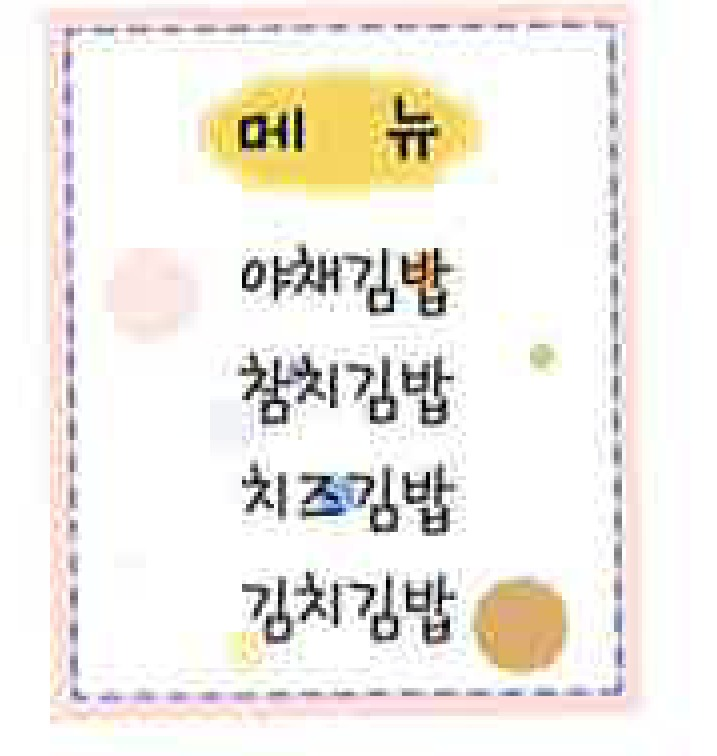
\includegraphics[width=0.92\linewidth]{figures/fig-47-11.jpg}\end{minipage}\par
}\vspace{8mm}
\setcounter{dmproblemcount}{11}\dmpnum{47-12}{% id: 47-12
% book: 베이직쎈 확률과 통계 · 03 확률의 뜻과 활용
% section: 유형 026 중복순열을 이용하는 확률
% figure: none
% answer: 
% answer_source: 
% variant_level: 0 (원본 전사)
% 이 파일은 build.mjs 가 items.json 에서 만든다. 고칠 때는 items.json 을 고친다.
\smash{\raisebox{1.5mm}{\dmkichul{베이직쎈 확률과 통계 47쪽 12번}}}
사과, 귤, 감, 복숭아, 키위, 망고, 배가 각각 1개씩 있다. 이 7개의 과일을 3개의 그릇 $\mathrm{A}$, $\mathrm{B}$, $\mathrm{C}$에 남김없이 담으려고 할 때, 사과, 복숭아, 망고가 그릇 $\mathrm{A}$에 담길 확률은? \dmcondfill{과일을 하나도 담지 않은 그릇이 있을 수도 있다.}{}
\dmchoicesauto{\rule[-3ex]{0pt}{8ex}}{$\dfrac{1}{27}$}{$\dfrac{2}{27}$}{$\dfrac{1}{9}$}{$\dfrac{4}{27}$}{$\dfrac{5}{27}$}
}\vspace{8mm}
\setcounter{dmproblemcount}{12}\dmpnum{48-13}{% id: 48-13
% book: 베이직쎈 확률과 통계 · 03 확률의 뜻과 활용
% section: 유형 026 중복순열을 이용하는 확률
% figure: none
% answer: 
% answer_source: 
% variant_level: 0 (원본 전사)
% 이 파일은 build.mjs 가 items.json 에서 만든다. 고칠 때는 items.json 을 고친다.
\smash{\raisebox{1.5mm}{\dmkichul{베이직쎈 확률과 통계 48쪽 13번}}}
$1$부터 $8$까지의 자연수에서 중복을 허용하여 4개를 뽑아 네 자리 자연수를 만들 때, 그 수가 짝수일 확률은?
\dmchoicesauto{\rule[-3ex]{0pt}{8ex}}{$\dfrac{15}{32}$}{$\dfrac{1}{2}$}{$\dfrac{17}{32}$}{$\dfrac{9}{16}$}{$\dfrac{19}{32}$}
}\vspace{8mm}
\setcounter{dmproblemcount}{13}\dmpnum{48-14}{% id: 48-14
% book: 베이직쎈 확률과 통계 · 03 확률의 뜻과 활용
% section: 유형 026 중복순열을 이용하는 확률
% figure: none
% answer: 
% answer_source: 
% variant_level: 0 (원본 전사)
% 이 파일은 build.mjs 가 items.json 에서 만든다. 고칠 때는 items.json 을 고친다.
\smash{\raisebox{1.5mm}{\dmkichul{베이직쎈 확률과 통계 48쪽 14번}}}
두 집합 $X=\{1{,}\mkern3mu\mathopen{}2{,}\mkern3mu\mathopen{}3\}$, $Y=\{a{,}\mkern3mu\mathopen{}b{,}\mkern3mu\mathopen{}c\}$에 대하여 $X$에서 $Y$로의 함수 중에서 임의로 택한 하나의 함수를 $f$라 할 때, $f$가 일대일대응일 확률을 구하시오.
}\vspace{8mm}
\dmsection{유형 027 같은 것이 있는 순열을 이용하는 확률}
\setcounter{dmproblemcount}{14}\dmpnum{48-15}{% id: 48-15
% book: 베이직쎈 확률과 통계 · 03 확률의 뜻과 활용
% section: 유형 027 같은 것이 있는 순열을 이용하는 확률
% figure: none
% answer: 
% answer_source: 
% variant_level: 0 (원본 전사)
% 이 파일은 build.mjs 가 items.json 에서 만든다. 고칠 때는 items.json 을 고친다.
\smash{\raisebox{1.5mm}{\dmkichul{베이직쎈 확률과 통계 48쪽 15번}}}
apple에 있는 5개의 문자를 일렬로 나열할 때, 양 끝에 모음이 올 확률은?
\dmchoicesauto{\rule[-3ex]{0pt}{8ex}}{$\dfrac{1}{10}$}{$\dfrac{1}{5}$}{$\dfrac{3}{10}$}{$\dfrac{2}{5}$}{$\dfrac{1}{2}$}
}\vspace{8mm}
\setcounter{dmproblemcount}{15}\dmpnum{48-16}{% id: 48-16
% book: 베이직쎈 확률과 통계 · 03 확률의 뜻과 활용
% section: 유형 027 같은 것이 있는 순열을 이용하는 확률
% figure: none
% answer: 
% answer_source: 
% variant_level: 0 (원본 전사)
% 이 파일은 build.mjs 가 items.json 에서 만든다. 고칠 때는 items.json 을 고친다.
\smash{\raisebox{1.5mm}{\dmkichul{베이직쎈 확률과 통계 48쪽 16번}}}
4개의 문자 $\mathrm{A}$, $\mathrm{A}$, $\mathrm{B}$, $\mathrm{B}$와 3개의 숫자 $1$, $2$, $3$을 일렬로 나열할 때, 숫자끼리 이웃할 확률은?
\dmchoicesauto{\rule[-3ex]{0pt}{8ex}}{$\dfrac{1}{21}$}{$\dfrac{2}{21}$}{$\dfrac{1}{7}$}{$\dfrac{4}{21}$}{$\dfrac{5}{21}$}
}\vspace{8mm}
\setcounter{dmproblemcount}{16}\dmpnum{48-17}{% id: 48-17
% book: 베이직쎈 확률과 통계 · 03 확률의 뜻과 활용
% section: 유형 027 같은 것이 있는 순열을 이용하는 확률
% figure: none
% answer: 
% answer_source: 
% variant_level: 0 (원본 전사)
% 이 파일은 build.mjs 가 items.json 에서 만든다. 고칠 때는 items.json 을 고친다.
\smash{\raisebox{1.5mm}{\dmkichul{베이직쎈 확률과 통계 48쪽 17번}}}
positive에 있는 8개의 문자를 일렬로 나열할 때, 모음을 알파벳 순서로 나열할 확률을 구하시오.
}\vspace{8mm}
\setcounter{dmproblemcount}{17}\dmpnum{48-18}{% id: 48-18
% book: 베이직쎈 확률과 통계 · 03 확률의 뜻과 활용
% section: 유형 027 같은 것이 있는 순열을 이용하는 확률
% figure: tikz:fig-48-18
% answer: 
% answer_source: 
% variant_level: 0 (원본 전사)
% 이 파일은 build.mjs 가 items.json 에서 만든다. 고칠 때는 items.json 을 고친다.
\smash{\raisebox{1.5mm}{\dmkichul{베이직쎈 확률과 통계 48쪽 18번}}}
\noindent\begin{minipage}[t]{0.58\linewidth}\vspace{0pt}\raggedright 오른쪽 그림과 같은 도로망이 있다. $\mathrm{A}$에서 $\mathrm{B}$까지 최단 거리로 갈 때, $\mathrm{P}$를 거쳐 갈 확률을 구하시오. \dmcondfill{각 경로를 택할 확률은 같은 것으로 생각한다.}{}\end{minipage}\hfill\begin{minipage}[t]{0.4\linewidth}\vspace{0pt}\centering \resizebox{\ifdim\width>\linewidth\linewidth\else\width\fi}{!}{% 유형 027 48-18(인쇄 48쪽) — 가로 6칸 · 세로 4칸 도로망. A 는 왼쪽 위 꼭짓점, B 는 오른쪽 아래 꼭짓점,
%   P 는 A 에서 오른쪽 1칸 · 아래 2칸 지점. 스캔 화질이 낮아 TikZ 로 다시 그림.
% 점 크기: 정점 2.2pt · 파생점 2pt. 답(경우의 수·확률)은 그림에 넣지 않는다.
\begin{tikzpicture}[scale=0.42, line width=0.5pt]
  \draw[line width=0.5pt] (0,0) grid (6,4);
  \coordinate (A) at (0,4);
  \coordinate (B) at (6,0);
  \coordinate (P) at (1,2);
  \fill (A) circle (2.2pt);
  \fill (B) circle (2.2pt);
  \fill (P) circle (2pt);
  \node[left, font=\small] at (A) {$\mathrm{A}$};
  \node[right, font=\small] at (B) {$\mathrm{B}$};
  \node[above left=-2pt and -2pt, font=\small] at (P) {$\mathrm{P}$};
\end{tikzpicture}
}\end{minipage}\par
}\vspace{8mm}
\dmsection{유형 028 조합을 이용하는 확률}
\setcounter{dmproblemcount}{18}\dmpnum{49-19}{% id: 49-19
% book: 베이직쎈 확률과 통계 · 03 확률의 뜻과 활용
% section: 유형 028 조합을 이용하는 확률
% figure: none
% answer: 
% answer_source: 
% variant_level: 0 (원본 전사)
% 이 파일은 build.mjs 가 items.json 에서 만든다. 고칠 때는 items.json 을 고친다.
\smash{\raisebox{1.5mm}{\dmkichul{베이직쎈 확률과 통계 49쪽 19번}}}
흰 공 5개와 검은 공 3개가 들어 있는 주머니에서 임의로 2개의 공을 동시에 꺼낼 때, 흰 공 1개와 검은 공 1개를 꺼낼 확률을 구하시오.
}\vspace{8mm}
\setcounter{dmproblemcount}{19}\dmpnum{49-20}{% id: 49-20
% book: 베이직쎈 확률과 통계 · 03 확률의 뜻과 활용
% section: 유형 028 조합을 이용하는 확률
% figure: none
% answer: 
% answer_source: 
% variant_level: 0 (원본 전사)
% 이 파일은 build.mjs 가 items.json 에서 만든다. 고칠 때는 items.json 을 고친다.
\smash{\raisebox{1.5mm}{\dmkichul{베이직쎈 확률과 통계 49쪽 20번}}}
은정이와 민욱이를 포함한 7명의 학생 중에서 임의로 3명의 대표를 뽑을 때, 은정이는 포함되고 민욱이는 포함되지 않을 확률은?
\begin{choicesii}{\rule[-3ex]{0pt}{8ex}$\dfrac{1}{14}$}{\rule[-3ex]{0pt}{8ex}$\dfrac{1}{7}$}{\rule[-3ex]{0pt}{8ex}$\dfrac{3}{14}$}{\rule[-3ex]{0pt}{8ex}$\dfrac{2}{7}$}{\rule[-3ex]{0pt}{8ex}$\dfrac{5}{14}$}\end{choicesii}
}\vspace{8mm}
\vspace{3mm}\setcounter{dmproblemcount}{20}\dmpnum{49-21}{% id: 49-21
% book: 베이직쎈 확률과 통계 · 03 확률의 뜻과 활용
% section: 유형 028 조합을 이용하는 확률
% figure: none
% answer: 
% answer_source: 
% variant_level: 0 (원본 전사)
% 이 파일은 build.mjs 가 items.json 에서 만든다. 고칠 때는 items.json 을 고친다.
\smash{\raisebox{4.5mm}{\dmkichul{베이직쎈 확률과 통계 49쪽 21번}}}
$n$개의 당첨 제비를 포함한 10개의 제비 중에서 임의로 2개의 제비를 동시에 뽑을 때, 2개 모두 당첨 제비일 확률은 $\dfrac{1}{15}$이다. 이때 $n$의 값을 구하시오. \dmcondfill{$n\ge 2$}{}
}\vspace{8mm}
\setcounter{dmproblemcount}{21}\dmpnum{49-22}{% id: 49-22
% book: 베이직쎈 확률과 통계 · 03 확률의 뜻과 활용
% section: 유형 028 조합을 이용하는 확률
% figure: none
% answer: 
% answer_source: 
% variant_level: 0 (원본 전사)
% 이 파일은 build.mjs 가 items.json 에서 만든다. 고칠 때는 items.json 을 고친다.
\smash{\raisebox{1.5mm}{\dmkichul{베이직쎈 확률과 통계 49쪽 22번}}}
1부터 6까지의 자연수가 각각 하나씩 적힌 6장의 카드 중에서 임의로 2장의 카드를 동시에 뽑을 때, 뽑힌 카드에 적힌 두 수의 합이 짝수일 확률은?
\begin{choicesii}{\rule[-3ex]{0pt}{8ex}$\dfrac{2}{15}$}{\rule[-3ex]{0pt}{8ex}$\dfrac{1}{5}$}{\rule[-3ex]{0pt}{8ex}$\dfrac{4}{15}$}{\rule[-3ex]{0pt}{8ex}$\dfrac{1}{3}$}{\rule[-3ex]{0pt}{8ex}$\dfrac{2}{5}$}\end{choicesii}
}\vspace{8mm}
\setcounter{dmproblemcount}{22}\dmpnum{49-23}{% id: 49-23
% book: 베이직쎈 확률과 통계 · 03 확률의 뜻과 활용
% section: 유형 028 조합을 이용하는 확률
% figure: tikz:fig-49-23
% answer: 
% answer_source: 
% variant_level: 0 (원본 전사)
% 이 파일은 build.mjs 가 items.json 에서 만든다. 고칠 때는 items.json 을 고친다.
\smash{\raisebox{1.5mm}{\dmkichul{베이직쎈 확률과 통계 49쪽 23번}}}
\noindent\begin{minipage}[t]{0.58\linewidth}\vspace{0pt}\raggedright 오른쪽 그림과 같이 원 위에 같은 간격으로 놓인 8개의 점 중에서 임의로 3개의 점을 택하여 그 3개의 점을 꼭짓점으로 하는 삼각형을 만들 때, 다음을 구하시오.\end{minipage}\hfill\begin{minipage}[t]{0.4\linewidth}\vspace{0pt}\centering \resizebox{\ifdim\width>\linewidth\linewidth\else\width\fi}{!}{% 유형 028 49-23(인쇄 49쪽) — 원 위에 같은 간격으로 놓인 8개의 점. 스캔 화질이 낮아 TikZ 로 다시 그림.
% 원문대로 점만 찍고 지름·삼각형은 그리지 않는다(직각삼각형의 개수가 그림에서 읽히지 않게). 라벨은 원문에 없다.
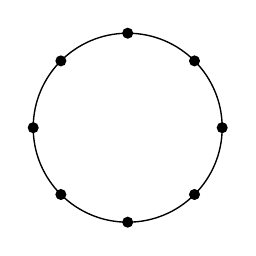
\begin{tikzpicture}[scale=1, line width=0.5pt]
  \draw (0,0) circle (1.2);
  \foreach \a in {0,45,...,315} { \fill (\a:1.2) circle (2pt); }
\end{tikzpicture}
}\end{minipage}\par
\dmsubprob{1} 만들 수 있는 삼각형의 개수
\dmsubprob{2} 만들 수 있는 직각삼각형의 개수
\dmsubprob{3} 만든 삼각형이 직각삼각형일 확률
}\vspace{8mm}
\dmsection{유형 029 통계적 확률}
\setcounter{dmproblemcount}{23}\dmpnum{49-24}{% id: 49-24
% book: 베이직쎈 확률과 통계 · 03 확률의 뜻과 활용
% section: 유형 029 통계적 확률
% figure: none
% answer: 
% answer_source: 
% variant_level: 0 (원본 전사)
% 이 파일은 build.mjs 가 items.json 에서 만든다. 고칠 때는 items.json 을 고친다.
\smash{\raisebox{1.5mm}{\dmkichul{베이직쎈 확률과 통계 49쪽 24번}}}
어느 양계장에서 달걀 1000개 중 850개가 부화에 성공했다고 한다. 같은 조건에서 달걀 한 개를 부화시킬 때, 이 달걀이 부화에 성공할 확률을 구하시오.
}\vspace{8mm}
\setcounter{dmproblemcount}{24}\dmpnum{50-25}{% id: 50-25
% book: 베이직쎈 확률과 통계 · 03 확률의 뜻과 활용
% section: 유형 029 통계적 확률
% figure: none
% answer: 
% answer_source: 
% variant_level: 0 (원본 전사)
% 이 파일은 build.mjs 가 items.json 에서 만든다. 고칠 때는 items.json 을 고친다.
\smash{\raisebox{1.5mm}{\dmkichul{베이직쎈 확률과 통계 50쪽 25번}}}
어느 질병에 걸린 400명의 환자에게 $\mathrm{A}$ 치료제를 투여한 결과 250명이 완치되었다고 한다. 같은 질병에 걸린 환자에게 $\mathrm{A}$ 치료제를 투여할 때, 이 환자가 완치될 확률은?
\begin{choicesii}{\rule[-3ex]{0pt}{8ex}$\dfrac{3}{5}$}{\rule[-3ex]{0pt}{8ex}$\dfrac{5}{8}$}{\rule[-3ex]{0pt}{8ex}$\dfrac{13}{20}$}{\rule[-3ex]{0pt}{8ex}$\dfrac{7}{10}$}{\rule[-3ex]{0pt}{8ex}$\dfrac{3}{4}$}\end{choicesii}
}\vspace{8mm}
\setcounter{dmproblemcount}{25}\dmpnum{50-26}{% id: 50-26
% book: 베이직쎈 확률과 통계 · 03 확률의 뜻과 활용
% section: 유형 029 통계적 확률
% figure: none
% answer: 
% answer_source: 
% variant_level: 0 (원본 전사)
% 이 파일은 build.mjs 가 items.json 에서 만든다. 고칠 때는 items.json 을 고친다.
\smash{\raisebox{1.5mm}{\dmkichul{베이직쎈 확률과 통계 50쪽 26번}}}
다음은 어느 사격 선수가 10점이 만점인 과녁에 총을 100번 쏘아 6점 이상을 맞힌 횟수를 조사하여 나타낸 표이다. 이 선수가 총을 한 번 쏠 때, 9점 이상을 맞힐 확률은?\par\smallskip\dispeq{\begin{tabular}{|c|c|c|c|c|c|}\hline 점수 & 6점 & 7점 & 8점 & 9점 & 10점 \\ \hline 횟수 & 7 & 12 & 23 & 28 & 10 \\ \hline\end{tabular}}\par\smallskip\noindent
\begin{choicesii}{\rule[-3ex]{0pt}{8ex}$\dfrac{19}{50}$}{\rule[-3ex]{0pt}{8ex}$\dfrac{39}{100}$}{\rule[-3ex]{0pt}{8ex}$\dfrac{2}{5}$}{\rule[-3ex]{0pt}{8ex}$\dfrac{41}{100}$}{\rule[-3ex]{0pt}{8ex}$\dfrac{21}{50}$}\end{choicesii}
}\vspace{8mm}
\setcounter{dmproblemcount}{26}\dmpnum{50-27}{% id: 50-27
% book: 베이직쎈 확률과 통계 · 03 확률의 뜻과 활용
% section: 유형 029 통계적 확률
% figure: none
% answer: 
% answer_source: 
% variant_level: 0 (원본 전사)
% 이 파일은 build.mjs 가 items.json 에서 만든다. 고칠 때는 items.json 을 고친다.
\smash{\raisebox{1.5mm}{\dmkichul{베이직쎈 확률과 통계 50쪽 27번}}}
주머니 속에 흰 공 $n$개, 노란 공 33개가 들어 있다. 이 주머니에서 임의로 한 개의 공을 꺼내어 색을 확인하고 다시 넣는 시행을 여러 번 반복했더니 15번에 4번 꼴로 흰 공이 나왔다. 이때 $n$의 값을 구하시오.
}\vspace{8mm}
\dmsection{유형 030 확률의 기본 성질}
\setcounter{dmproblemcount}{27}\dmpnum{50-28}{% id: 50-28
% book: 베이직쎈 확률과 통계 · 03 확률의 뜻과 활용
% section: 유형 030 확률의 기본 성질
% figure: none
% answer: 
% answer_source: 
% variant_level: 0 (원본 전사)
% 이 파일은 build.mjs 가 items.json 에서 만든다. 고칠 때는 items.json 을 고친다.
\smash{\raisebox{1.5mm}{\dmkichul{베이직쎈 확률과 통계 50쪽 28번}}}
빨간 구슬 1개와 검은 구슬 5개가 들어 있는 상자에서 임의로 2개의 구슬을 동시에 꺼낼 때, 2개 모두 빨간 구슬을 꺼낼 확률을 $p$, 적어도 1개는 검은 구슬을 꺼낼 확률을 $q$라 하자. 이때 $p$, $q$의 값을 구하시오.
}\vspace{8mm}
\setcounter{dmproblemcount}{28}\dmpnum{50-29}{% id: 50-29
% book: 베이직쎈 확률과 통계 · 03 확률의 뜻과 활용
% section: 유형 030 확률의 기본 성질
% figure: none
% answer: 
% answer_source: 
% variant_level: 0 (원본 전사)
% 이 파일은 build.mjs 가 items.json 에서 만든다. 고칠 때는 items.json 을 고친다.
\smash{\raisebox{1.5mm}{\dmkichul{베이직쎈 확률과 통계 50쪽 29번}}}
다음 중 표본공간 $S$의 두 사건 $A$, $B$에 대하여 옳지 \underline{않은} 것은? \dmcondfill{$\varnothing$는 절대로 일어나지 않는 사건이다.}{}
\begin{choicesv}{$0\le\mathrm{P}(\comp{A})\le 1$}{$\mathrm{P}(S)+\mathrm{P}(\varnothing)=1$}{$0\le\mathrm{P}(A\cap B)\le 1$}{$1\le\mathrm{P}(A\cup B)\le 2$}{$\mathrm{P}(A\cup\comp{A})=1$}\end{choicesv}
}\vspace{8mm}
\setcounter{dmproblemcount}{29}\dmpnum{50-30}{% id: 50-30
% book: 베이직쎈 확률과 통계 · 03 확률의 뜻과 활용
% section: 유형 030 확률의 기본 성질
% figure: none
% answer: 
% answer_source: 
% variant_level: 0 (원본 전사)
% 이 파일은 build.mjs 가 items.json 에서 만든다. 고칠 때는 items.json 을 고친다.
\smash{\raisebox{1.5mm}{\dmkichul{베이직쎈 확률과 통계 50쪽 30번}}}
서로 다른 두 개의 주사위를 동시에 던질 때,\par\smallskip\dispeq{$p=$(나온 두 눈의 수의 합이 1일 확률),}\par\dispeq{$q=$(나온 두 눈의 수의 차가 4 이상일 확률),}\par\dispeq{$r=$(나온 두 눈의 수의 곱이 36 이하일 확률)}\par\smallskip\noindent 이라 하자. 이때 $p+q+r$의 값은?
\begin{choicesii}{\rule[-3ex]{0pt}{8ex}$\dfrac{7}{6}$}{\rule[-3ex]{0pt}{8ex}$\dfrac{4}{3}$}{\rule[-3ex]{0pt}{8ex}$\dfrac{3}{2}$}{\rule[-3ex]{0pt}{8ex}$\dfrac{5}{3}$}{\rule[-3ex]{0pt}{8ex}$\dfrac{11}{6}$}\end{choicesii}
}\vspace{8mm}
\dmsection{개념 15 확률의 덧셈정리}
\dmpassage{두 사건 $A$, $B$가 다음을 만족시킬 때, $\mathrm{P}(A\cup B)$를 구하시오.}
\vspace{3mm}\setcounter{dmproblemcount}{0}\dmpnum{51-01}{% id: 51-01
% book: 베이직쎈 확률과 통계 · 03 확률의 뜻과 활용
% section: 개념 15 확률의 덧셈정리
% passage: 두 사건 $A$, $B$가 다음을 만족시킬 때, $\mathrm{P}(A\cup B)$를 구하시오.
% figure: none
% answer: 
% answer_source: 
% variant_level: 0 (원본 전사)
% 이 파일은 build.mjs 가 items.json 에서 만든다. 고칠 때는 items.json 을 고친다.
\smash{\raisebox{4.5mm}{\dmkichul{베이직쎈 확률과 통계 51쪽 01번}}}
$\mathrm{P}(A)=\dfrac{1}{2}$, $\mathrm{P}(B)=\dfrac{3}{4}$, $\mathrm{P}(A\cap B)=\dfrac{5}{12}$
}\vspace{8mm}
\vspace{3mm}\setcounter{dmproblemcount}{1}\dmpnum{51-02}{% id: 51-02
% book: 베이직쎈 확률과 통계 · 03 확률의 뜻과 활용
% section: 개념 15 확률의 덧셈정리
% passage: 두 사건 $A$, $B$가 다음을 만족시킬 때, $\mathrm{P}(A\cup B)$를 구하시오.
% figure: none
% answer: 
% answer_source: 
% variant_level: 0 (원본 전사)
% 이 파일은 build.mjs 가 items.json 에서 만든다. 고칠 때는 items.json 을 고친다.
\smash{\raisebox{4.5mm}{\dmkichul{베이직쎈 확률과 통계 51쪽 02번}}}
$\mathrm{P}(A)=\dfrac{1}{5}$, $\mathrm{P}(B)=\dfrac{3}{7}$, $\mathrm{P}(A\cap B)=\dfrac{2}{35}$
}\vspace{8mm}
\dmpassage{두 사건 $A$, $B$에 대하여 다음을 구하시오.}
\vspace{3mm}\setcounter{dmproblemcount}{2}\dmpnum{51-03}{% id: 51-03
% book: 베이직쎈 확률과 통계 · 03 확률의 뜻과 활용
% section: 개념 15 확률의 덧셈정리
% passage: 두 사건 $A$, $B$에 대하여 다음을 구하시오.
% figure: none
% answer: 
% answer_source: 
% variant_level: 0 (원본 전사)
% 이 파일은 build.mjs 가 items.json 에서 만든다. 고칠 때는 items.json 을 고친다.
\smash{\raisebox{4.5mm}{\dmkichul{베이직쎈 확률과 통계 51쪽 03번}}}
$\mathrm{P}(A)=\dfrac{2}{3}$, $\mathrm{P}(B)=\dfrac{2}{5}$, $\mathrm{P}(A\cup B)=\dfrac{5}{6}$일 때, $\mathrm{P}(A\cap B)$
}\vspace{8mm}
\vspace{3mm}\setcounter{dmproblemcount}{3}\dmpnum{51-04}{% id: 51-04
% book: 베이직쎈 확률과 통계 · 03 확률의 뜻과 활용
% section: 개념 15 확률의 덧셈정리
% passage: 두 사건 $A$, $B$에 대하여 다음을 구하시오.
% figure: none
% answer: 
% answer_source: 
% variant_level: 0 (원본 전사)
% 이 파일은 build.mjs 가 items.json 에서 만든다. 고칠 때는 items.json 을 고친다.
\smash{\raisebox{4.5mm}{\dmkichul{베이직쎈 확률과 통계 51쪽 04번}}}
$\mathrm{P}(A)=\dfrac{1}{3}$, $\mathrm{P}(B)=\dfrac{2}{5}$, $\mathrm{P}(A\cup B)=\dfrac{2}{3}$일 때, $\mathrm{P}(A\cap B)$
}\vspace{8mm}
\vspace{3mm}\setcounter{dmproblemcount}{4}\dmpnum{51-05}{% id: 51-05
% book: 베이직쎈 확률과 통계 · 03 확률의 뜻과 활용
% section: 개념 15 확률의 덧셈정리
% passage: 두 사건 $A$, $B$에 대하여 다음을 구하시오.
% figure: none
% answer: 
% answer_source: 
% variant_level: 0 (원본 전사)
% 이 파일은 build.mjs 가 items.json 에서 만든다. 고칠 때는 items.json 을 고친다.
\smash{\raisebox{4.5mm}{\dmkichul{베이직쎈 확률과 통계 51쪽 05번}}}
$\mathrm{P}(A)=\dfrac{1}{4}$, $\mathrm{P}(A\cap B)=\dfrac{1}{12}$, $\mathrm{P}(A\cup B)=\dfrac{7}{12}$일 때, $\mathrm{P}(B)$
}\vspace{8mm}
\vspace{3mm}\setcounter{dmproblemcount}{5}\dmpnum{51-06}{% id: 51-06
% book: 베이직쎈 확률과 통계 · 03 확률의 뜻과 활용
% section: 개념 15 확률의 덧셈정리
% passage: 두 사건 $A$, $B$에 대하여 다음을 구하시오.
% figure: none
% answer: 
% answer_source: 
% variant_level: 0 (원본 전사)
% 이 파일은 build.mjs 가 items.json 에서 만든다. 고칠 때는 items.json 을 고친다.
\smash{\raisebox{4.5mm}{\dmkichul{베이직쎈 확률과 통계 51쪽 06번}}}
$\mathrm{P}(B)=\dfrac{1}{2}$, $\mathrm{P}(A\cap B)=\dfrac{4}{9}$, $\mathrm{P}(A\cup B)=\dfrac{8}{9}$일 때, $\mathrm{P}(A)$
}\vspace{8mm}
\dmpassage{두 사건 $A$, $B$가 서로 배반사건이고 다음을 만족시킬 때, $\mathrm{P}(A\cup B)$를 구하시오.}
\vspace{3mm}\setcounter{dmproblemcount}{6}\dmpnum{51-07}{% id: 51-07
% book: 베이직쎈 확률과 통계 · 03 확률의 뜻과 활용
% section: 개념 15 확률의 덧셈정리
% passage: 두 사건 $A$, $B$가 서로 배반사건이고 다음을 만족시킬 때, $\mathrm{P}(A\cup B)$를 구하시오.
% figure: none
% answer: 
% answer_source: 
% variant_level: 0 (원본 전사)
% 이 파일은 build.mjs 가 items.json 에서 만든다. 고칠 때는 items.json 을 고친다.
\smash{\raisebox{4.5mm}{\dmkichul{베이직쎈 확률과 통계 51쪽 07번}}}
$\mathrm{P}(A)=\dfrac{2}{3}$, $\mathrm{P}(B)=\dfrac{1}{6}$
}\vspace{8mm}
\vspace{3mm}\setcounter{dmproblemcount}{7}\dmpnum{51-08}{% id: 51-08
% book: 베이직쎈 확률과 통계 · 03 확률의 뜻과 활용
% section: 개념 15 확률의 덧셈정리
% passage: 두 사건 $A$, $B$가 서로 배반사건이고 다음을 만족시킬 때, $\mathrm{P}(A\cup B)$를 구하시오.
% figure: none
% answer: 
% answer_source: 
% variant_level: 0 (원본 전사)
% 이 파일은 build.mjs 가 items.json 에서 만든다. 고칠 때는 items.json 을 고친다.
\smash{\raisebox{4.5mm}{\dmkichul{베이직쎈 확률과 통계 51쪽 08번}}}
$\mathrm{P}(A)=\dfrac{1}{4}$, $\mathrm{P}(B)=\dfrac{5}{8}$
}\vspace{8mm}
\dmpassage{두 사건 $A$, $B$가 서로 배반사건일 때, 다음을 구하시오.}
\vspace{3mm}\setcounter{dmproblemcount}{8}\dmpnum{51-09}{% id: 51-09
% book: 베이직쎈 확률과 통계 · 03 확률의 뜻과 활용
% section: 개념 15 확률의 덧셈정리
% passage: 두 사건 $A$, $B$가 서로 배반사건일 때, 다음을 구하시오.
% figure: none
% answer: 
% answer_source: 
% variant_level: 0 (원본 전사)
% 이 파일은 build.mjs 가 items.json 에서 만든다. 고칠 때는 items.json 을 고친다.
\smash{\raisebox{4.5mm}{\dmkichul{베이직쎈 확률과 통계 51쪽 09번}}}
$\mathrm{P}(A)=\dfrac{3}{7}$, $\mathrm{P}(A\cup B)=\dfrac{9}{14}$일 때, $\mathrm{P}(B)$
}\vspace{8mm}
\vspace{3mm}\setcounter{dmproblemcount}{9}\dmpnum{51-10}{% id: 51-10
% book: 베이직쎈 확률과 통계 · 03 확률의 뜻과 활용
% section: 개념 15 확률의 덧셈정리
% passage: 두 사건 $A$, $B$가 서로 배반사건일 때, 다음을 구하시오.
% figure: none
% answer: 
% answer_source: 
% variant_level: 0 (원본 전사)
% 이 파일은 build.mjs 가 items.json 에서 만든다. 고칠 때는 items.json 을 고친다.
\smash{\raisebox{4.5mm}{\dmkichul{베이직쎈 확률과 통계 51쪽 10번}}}
$\mathrm{P}(B)=\dfrac{3}{10}$, $\mathrm{P}(A\cup B)=\dfrac{4}{5}$일 때, $\mathrm{P}(A)$
}\vspace{8mm}
\setcounter{dmproblemcount}{10}\dmpnum{52-11}{% id: 52-11
% book: 베이직쎈 확률과 통계 · 03 확률의 뜻과 활용
% section: 개념 15 확률의 덧셈정리
% figure: none
% answer: 
% answer_source: 
% variant_level: 0 (원본 전사)
% 이 파일은 build.mjs 가 items.json 에서 만든다. 고칠 때는 items.json 을 고친다.
\smash{\raisebox{1.5mm}{\dmkichul{베이직쎈 확률과 통계 52쪽 11번}}}
한 개의 주사위를 던질 때, 짝수의 눈이 나오는 사건을 $A$, 6의 약수의 눈이 나오는 사건을 $B$라 하자. 다음을 구하시오.
\dmsubprob{1} $\mathrm{P}(A)$, $\mathrm{P}(B)$
\dmsubprob{2} $\mathrm{P}(A\cap B)$
\dmsubprob{3} $\mathrm{P}(A\cup B)$
}\vspace{8mm}
\setcounter{dmproblemcount}{11}\dmpnum{52-12}{% id: 52-12
% book: 베이직쎈 확률과 통계 · 03 확률의 뜻과 활용
% section: 개념 15 확률의 덧셈정리
% figure: none
% answer: 
% answer_source: 
% variant_level: 0 (원본 전사)
% 이 파일은 build.mjs 가 items.json 에서 만든다. 고칠 때는 items.json 을 고친다.
\smash{\raisebox{1.5mm}{\dmkichul{베이직쎈 확률과 통계 52쪽 12번}}}
서로 다른 두 개의 주사위를 동시에 던질 때, 다음을 구하시오.
\dmsubprob{1} 나온 두 눈의 수의 합이 7일 확률
\dmsubprob{2} 나온 두 눈의 수의 차가 3일 확률
\dmsubprob{3} 나온 두 눈의 수의 합이 7이고, 차가 3일 확률
\dmsubprob{4} 나온 두 눈의 수의 합이 7이거나 차가 3일 확률
}\vspace{8mm}
\setcounter{dmproblemcount}{12}\dmpnum{52-13}{% id: 52-13
% book: 베이직쎈 확률과 통계 · 03 확률의 뜻과 활용
% section: 개념 15 확률의 덧셈정리
% figure: none
% answer: 
% answer_source: 
% variant_level: 0 (원본 전사)
% 이 파일은 build.mjs 가 items.json 에서 만든다. 고칠 때는 items.json 을 고친다.
\smash{\raisebox{1.5mm}{\dmkichul{베이직쎈 확률과 통계 52쪽 13번}}}
서로 다른 두 개의 주사위를 동시에 던질 때, 나온 두 눈의 수가 서로 같거나 합이 4일 확률을 구하시오.
}\vspace{8mm}
\setcounter{dmproblemcount}{13}\dmpnum{52-14}{% id: 52-14
% book: 베이직쎈 확률과 통계 · 03 확률의 뜻과 활용
% section: 개념 15 확률의 덧셈정리
% figure: none
% answer: 
% answer_source: 
% variant_level: 0 (원본 전사)
% 이 파일은 build.mjs 가 items.json 에서 만든다. 고칠 때는 items.json 을 고친다.
\smash{\raisebox{1.5mm}{\dmkichul{베이직쎈 확률과 통계 52쪽 14번}}}
1부터 20까지의 자연수가 각각 하나씩 적힌 20개의 공이 들어 있는 상자에서 임의로 한 개의 공을 꺼낼 때, 다음을 구하시오.
\dmsubprob{1} 2의 배수가 적힌 공을 꺼낼 확률
\dmsubprob{2} 3의 배수가 적힌 공을 꺼낼 확률
\dmsubprob{3} 6의 배수가 적힌 공을 꺼낼 확률
\dmsubprob{4} 2의 배수 또는 3의 배수가 적힌 공을 꺼낼 확률
}\vspace{8mm}
\setcounter{dmproblemcount}{14}\dmpnum{52-15}{% id: 52-15
% book: 베이직쎈 확률과 통계 · 03 확률의 뜻과 활용
% section: 개념 15 확률의 덧셈정리
% figure: none
% answer: 
% answer_source: 
% variant_level: 0 (원본 전사)
% 이 파일은 build.mjs 가 items.json 에서 만든다. 고칠 때는 items.json 을 고친다.
\smash{\raisebox{1.5mm}{\dmkichul{베이직쎈 확률과 통계 52쪽 15번}}}
1부터 20까지의 자연수가 각각 하나씩 적힌 20개의 공이 들어 있는 상자에서 임의로 한 개의 공을 꺼낼 때, 3의 배수 또는 4의 배수가 적힌 공을 꺼낼 확률을 구하시오.
}\vspace{8mm}
\setcounter{dmproblemcount}{15}\dmpnum{52-16}{% id: 52-16
% book: 베이직쎈 확률과 통계 · 03 확률의 뜻과 활용
% section: 개념 15 확률의 덧셈정리
% figure: none
% answer: 
% answer_source: 
% variant_level: 0 (원본 전사)
% 이 파일은 build.mjs 가 items.json 에서 만든다. 고칠 때는 items.json 을 고친다.
\smash{\raisebox{1.5mm}{\dmkichul{베이직쎈 확률과 통계 52쪽 16번}}}
1부터 30까지의 자연수가 각각 하나씩 적힌 30장의 카드 중에서 임의로 한 장의 카드를 뽑을 때, 다음을 구하시오.
\dmsubprob{1} 10 이하인 수가 적힌 카드를 뽑을 확률
\dmsubprob{2} 23 이상인 수가 적힌 카드를 뽑을 확률
\dmsubprob{3} 10 이하인 수 또는 23 이상인 수가 적힌 카드를 뽑을 확률
}\vspace{8mm}
\setcounter{dmproblemcount}{16}\dmpnum{52-17}{% id: 52-17
% book: 베이직쎈 확률과 통계 · 03 확률의 뜻과 활용
% section: 개념 15 확률의 덧셈정리
% figure: none
% answer: 
% answer_source: 
% variant_level: 0 (원본 전사)
% 이 파일은 build.mjs 가 items.json 에서 만든다. 고칠 때는 items.json 을 고친다.
\smash{\raisebox{1.5mm}{\dmkichul{베이직쎈 확률과 통계 52쪽 17번}}}
1부터 30까지의 자연수가 각각 하나씩 적힌 30장의 카드 중에서 임의로 한 장의 카드를 뽑을 때, 5의 배수 또는 8의 약수가 적힌 카드를 뽑을 확률을 구하시오.
}\vspace{8mm}
\dmsection{개념 16 여사건의 확률}
\dmpassage{두 사건 $A$, $B$에 대하여 다음을 구하시오.}
\vspace{3mm}\setcounter{dmproblemcount}{17}\dmpnum{53-18}{% id: 53-18
% book: 베이직쎈 확률과 통계 · 03 확률의 뜻과 활용
% section: 개념 16 여사건의 확률
% passage: 두 사건 $A$, $B$에 대하여 다음을 구하시오.
% figure: none
% answer: 
% answer_source: 
% variant_level: 0 (원본 전사)
% 이 파일은 build.mjs 가 items.json 에서 만든다. 고칠 때는 items.json 을 고친다.
\smash{\raisebox{4.5mm}{\dmkichul{베이직쎈 확률과 통계 53쪽 18번}}}
$\mathrm{P}(A)=\dfrac{3}{5}$일 때, $\mathrm{P}(\comp{A})$
}\vspace{8mm}
\vspace{3mm}\setcounter{dmproblemcount}{18}\dmpnum{53-19}{% id: 53-19
% book: 베이직쎈 확률과 통계 · 03 확률의 뜻과 활용
% section: 개념 16 여사건의 확률
% passage: 두 사건 $A$, $B$에 대하여 다음을 구하시오.
% figure: none
% answer: 
% answer_source: 
% variant_level: 0 (원본 전사)
% 이 파일은 build.mjs 가 items.json 에서 만든다. 고칠 때는 items.json 을 고친다.
\smash{\raisebox{4.5mm}{\dmkichul{베이직쎈 확률과 통계 53쪽 19번}}}
$\mathrm{P}(A)=\dfrac{1}{7}$일 때, $\mathrm{P}(\comp{A})$
}\vspace{8mm}
\vspace{5mm}\setcounter{dmproblemcount}{19}\dmpnum{53-20}{% id: 53-20
% book: 베이직쎈 확률과 통계 · 03 확률의 뜻과 활용
% section: 개념 16 여사건의 확률
% passage: 두 사건 $A$, $B$에 대하여 다음을 구하시오.
% figure: none
% answer: 
% answer_source: 
% variant_level: 0 (원본 전사)
% 이 파일은 build.mjs 가 items.json 에서 만든다. 고칠 때는 items.json 을 고친다.
\smash{\raisebox{6.5mm}{\dmkichul{베이직쎈 확률과 통계 53쪽 20번}}}
$\mathrm{P}(A\cup B)=\dfrac{2}{3}$일 때,\par\smallskip\dispeq{$\begin{aligned}\mathrm{P}(\comp{A}\cap\comp{B})&=\mathrm{P}((\blank[3em])^{\mathrm{c}})\\ &=1-\mathrm{P}(\blank[3em])\\ &=1-\blank[1.5em]=\blank[1.5em]\end{aligned}$}\par\smallskip\noindent
}\vspace{8mm}
\vspace{3mm}\setcounter{dmproblemcount}{20}\dmpnum{53-21}{% id: 53-21
% book: 베이직쎈 확률과 통계 · 03 확률의 뜻과 활용
% section: 개념 16 여사건의 확률
% passage: 두 사건 $A$, $B$에 대하여 다음을 구하시오.
% figure: none
% answer: 
% answer_source: 
% variant_level: 0 (원본 전사)
% 이 파일은 build.mjs 가 items.json 에서 만든다. 고칠 때는 items.json 을 고친다.
\smash{\raisebox{4.5mm}{\dmkichul{베이직쎈 확률과 통계 53쪽 21번}}}
$\mathrm{P}(A\cup B)=\dfrac{4}{9}$일 때, $\mathrm{P}(\comp{A}\cap\comp{B})$
}\vspace{8mm}
\vspace{3mm}\setcounter{dmproblemcount}{21}\dmpnum{53-22}{% id: 53-22
% book: 베이직쎈 확률과 통계 · 03 확률의 뜻과 활용
% section: 개념 16 여사건의 확률
% passage: 두 사건 $A$, $B$에 대하여 다음을 구하시오.
% figure: none
% answer: 
% answer_source: 
% variant_level: 0 (원본 전사)
% 이 파일은 build.mjs 가 items.json 에서 만든다. 고칠 때는 items.json 을 고친다.
\smash{\raisebox{4.5mm}{\dmkichul{베이직쎈 확률과 통계 53쪽 22번}}}
$\mathrm{P}(A\cap B)=\dfrac{1}{4}$일 때, $\mathrm{P}(\comp{A}\cup\comp{B})$
}\vspace{8mm}
\vspace{3mm}\setcounter{dmproblemcount}{22}\dmpnum{53-23}{% id: 53-23
% book: 베이직쎈 확률과 통계 · 03 확률의 뜻과 활용
% section: 개념 16 여사건의 확률
% passage: 두 사건 $A$, $B$에 대하여 다음을 구하시오.
% figure: none
% answer: 
% answer_source: 
% variant_level: 0 (원본 전사)
% 이 파일은 build.mjs 가 items.json 에서 만든다. 고칠 때는 items.json 을 고친다.
\smash{\raisebox{4.5mm}{\dmkichul{베이직쎈 확률과 통계 53쪽 23번}}}
$\mathrm{P}(A\cap B)=\dfrac{3}{8}$일 때, $\mathrm{P}(\comp{A}\cup\comp{B})$
}\vspace{8mm}
\dmpassage{다음을 구하시오.}
\setcounter{dmproblemcount}{23}\dmpnum{53-24}{% id: 53-24
% book: 베이직쎈 확률과 통계 · 03 확률의 뜻과 활용
% section: 개념 16 여사건의 확률
% passage: 다음을 구하시오.
% figure: none
% answer: 
% answer_source: 
% variant_level: 0 (원본 전사)
% 이 파일은 build.mjs 가 items.json 에서 만든다. 고칠 때는 items.json 을 고친다.
\smash{\raisebox{1.5mm}{\dmkichul{베이직쎈 확률과 통계 53쪽 24번}}}
서로 다른 두 개의 주사위를 동시에 던질 때, 나온 두 눈의 수가 서로 다를 확률
}\vspace{8mm}
\setcounter{dmproblemcount}{24}\dmpnum{53-25}{% id: 53-25
% book: 베이직쎈 확률과 통계 · 03 확률의 뜻과 활용
% section: 개념 16 여사건의 확률
% passage: 다음을 구하시오.
% figure: none
% answer: 
% answer_source: 
% variant_level: 0 (원본 전사)
% 이 파일은 build.mjs 가 items.json 에서 만든다. 고칠 때는 items.json 을 고친다.
\smash{\raisebox{1.5mm}{\dmkichul{베이직쎈 확률과 통계 53쪽 25번}}}
흰 공 3개, 파란 공 2개가 들어 있는 주머니에서 임의로 2개의 공을 동시에 꺼낼 때, 적어도 한 개는 파란 공을 꺼낼 확률
}\vspace{8mm}
\setcounter{dmproblemcount}{25}\dmpnum{53-26}{% id: 53-26
% book: 베이직쎈 확률과 통계 · 03 확률의 뜻과 활용
% section: 개념 16 여사건의 확률
% passage: 다음을 구하시오.
% figure: none
% answer: 
% answer_source: 
% variant_level: 0 (원본 전사)
% 이 파일은 build.mjs 가 items.json 에서 만든다. 고칠 때는 items.json 을 고친다.
\smash{\raisebox{1.5mm}{\dmkichul{베이직쎈 확률과 통계 53쪽 26번}}}
남학생 2명, 여학생 4명 중에서 임의로 2명의 대표를 뽑을 때, 적어도 한 명은 여학생일 확률
}\vspace{8mm}
\setcounter{dmproblemcount}{26}\dmpnum{53-27}{% id: 53-27
% book: 베이직쎈 확률과 통계 · 03 확률의 뜻과 활용
% section: 개념 16 여사건의 확률
% passage: 다음을 구하시오.
% figure: none
% answer: 
% answer_source: 
% variant_level: 0 (원본 전사)
% 이 파일은 build.mjs 가 items.json 에서 만든다. 고칠 때는 items.json 을 고친다.
\smash{\raisebox{1.5mm}{\dmkichul{베이직쎈 확률과 통계 53쪽 27번}}}
서로 다른 4개의 동전을 동시에 던질 때, 앞면이 3개 이하 나올 확률
}\vspace{8mm}
\dmsection{유형 031 확률의 계산}
\vspace{3mm}\setcounter{dmproblemcount}{0}\dmpnum{54-01}{% id: 54-01
% book: 베이직쎈 확률과 통계 · 03 확률의 뜻과 활용
% section: 유형 031 확률의 계산
% figure: none
% answer: 
% answer_source: 
% variant_level: 0 (원본 전사)
% 이 파일은 build.mjs 가 items.json 에서 만든다. 고칠 때는 items.json 을 고친다.
\smash{\raisebox{4.5mm}{\dmkichul{베이직쎈 확률과 통계 54쪽 01번}}}
두 사건 $A$, $B$에 대하여 \par\smallskip\dispeq{$\mathrm{P}(A)=\dfrac{1}{3}$, $\mathrm{P}(A\cap B)=\dfrac{1}{6}$, $\mathrm{P}(A\cup B)=\dfrac{11}{12}$}\par\smallskip\noindent 일 때, $\mathrm{P}(\comp{B})$는?
\dmchoicesauto{\rule[-3ex]{0pt}{8ex}}{$\dfrac{1}{6}$}{$\dfrac{1}{4}$}{$\dfrac{1}{3}$}{$\dfrac{5}{12}$}{$\dfrac{1}{2}$}
}\vspace{8mm}
\vspace{3mm}\setcounter{dmproblemcount}{1}\dmpnum{54-02}{% id: 54-02
% book: 베이직쎈 확률과 통계 · 03 확률의 뜻과 활용
% section: 유형 031 확률의 계산
% figure: none
% answer: 
% answer_source: 
% variant_level: 0 (원본 전사)
% 이 파일은 build.mjs 가 items.json 에서 만든다. 고칠 때는 items.json 을 고친다.
\smash{\raisebox{4.5mm}{\dmkichul{베이직쎈 확률과 통계 54쪽 02번}}}
표본공간 $S$의 두 사건 $A$, $B$가 서로 배반사건이고 \par\smallskip\dispeq{$\mathrm{P}(B)=\dfrac{5}{8}$, $\mathrm{P}(A\cup B)=\mathrm{P}(S)$}\par\smallskip\noindent 일 때, $\mathrm{P}(A)$를 구하시오.
}\vspace{8mm}
\vspace{3mm}\setcounter{dmproblemcount}{2}\dmpnum{54-03}{% id: 54-03
% book: 베이직쎈 확률과 통계 · 03 확률의 뜻과 활용
% section: 유형 031 확률의 계산
% figure: none
% answer: 
% answer_source: 
% variant_level: 0 (원본 전사)
% 이 파일은 build.mjs 가 items.json 에서 만든다. 고칠 때는 items.json 을 고친다.
\smash{\raisebox{4.5mm}{\dmkichul{베이직쎈 확률과 통계 54쪽 03번}}}
두 사건 $A$, $B$가 서로 배반사건이고 \par\smallskip\dispeq{$\mathrm{P}(A\cup B)=\dfrac{3}{4}$, $\mathrm{P}(B)=\dfrac{1}{6}\mathrm{P}(A)$}\par\smallskip\noindent 일 때, $\mathrm{P}(A)$를 구하시오.
}\vspace{8mm}
\setcounter{dmproblemcount}{3}\dmpnum{54-04}{% id: 54-04
% book: 베이직쎈 확률과 통계 · 03 확률의 뜻과 활용
% section: 유형 031 확률의 계산
% figure: none
% answer: 
% answer_source: 
% variant_level: 0 (원본 전사)
% 이 파일은 build.mjs 가 items.json 에서 만든다. 고칠 때는 items.json 을 고친다.
\smash{\raisebox{1.5mm}{\dmkichul{베이직쎈 확률과 통계 54쪽 04번}}}
두 사건 $A$, $B$에 대하여 \par\smallskip\dispeq{$\mathrm{P}(A\cap B)=0.3$, $\mathrm{P}(A\cap \comp{B})=0.15$}\par\smallskip\noindent 일 때, $\mathrm{P}(\comp{A})$는?
\dmchoicesauto{}{$0.5$}{$0.55$}{$0.6$}{$0.65$}{$0.7$}
}\vspace{8mm}
\vspace{3mm}\setcounter{dmproblemcount}{4}\dmpnum{54-05}{% id: 54-05
% book: 베이직쎈 확률과 통계 · 03 확률의 뜻과 활용
% section: 유형 031 확률의 계산
% figure: none
% answer: 
% answer_source: 
% variant_level: 0 (원본 전사)
% 이 파일은 build.mjs 가 items.json 에서 만든다. 고칠 때는 items.json 을 고친다.
\smash{\raisebox{4.5mm}{\dmkichul{베이직쎈 확률과 통계 54쪽 05번}}}
두 사건 $A$, $B$에 대하여 \par\smallskip\dispeq{$\mathrm{P}(A)=\dfrac{2}{5}$, $\mathrm{P}(\comp{B})=\dfrac{7}{10}$, $\mathrm{P}(A\cup B)=\dfrac{1}{2}$}\par\smallskip\noindent 일 때, $\mathrm{P}(\comp{A}\cup \comp{B})$는?
\dmchoicesauto{\rule[-3ex]{0pt}{8ex}}{$\dfrac{1}{2}$}{$\dfrac{3}{5}$}{$\dfrac{7}{10}$}{$\dfrac{4}{5}$}{$\dfrac{9}{10}$}
}\vspace{8mm}
\vspace{3mm}\setcounter{dmproblemcount}{5}\dmpnum{54-06}{% id: 54-06
% book: 베이직쎈 확률과 통계 · 03 확률의 뜻과 활용
% section: 유형 031 확률의 계산
% figure: none
% answer: 
% answer_source: 
% variant_level: 0 (원본 전사)
% 이 파일은 build.mjs 가 items.json 에서 만든다. 고칠 때는 items.json 을 고친다.
\smash{\raisebox{4.5mm}{\dmkichul{베이직쎈 확률과 통계 54쪽 06번}}}
두 사건 $A$, $B$가 서로 배반사건이고 \par\smallskip\dispeq{$\mathrm{P}(A)=\dfrac{3}{5}$, $\mathrm{P}(A)+\mathrm{P}(B)=4\mathrm{P}(\comp{A}\cap \comp{B})$}\par\smallskip\noindent 일 때, $\mathrm{P}(B)$를 구하시오.
}\vspace{8mm}
\vspace{3mm}\setcounter{dmproblemcount}{6}\dmpnum{54-07}{% id: 54-07
% book: 베이직쎈 확률과 통계 · 03 확률의 뜻과 활용
% section: 유형 031 확률의 계산
% figure: none
% answer: 
% answer_source: 
% variant_level: 0 (원본 전사)
% 이 파일은 build.mjs 가 items.json 에서 만든다. 고칠 때는 items.json 을 고친다.
\smash{\raisebox{4.5mm}{\dmkichul{베이직쎈 확률과 통계 54쪽 07번}}}
표본공간 $S$의 두 사건 $A$, $B$가 서로 배반사건이고 $\mathrm{P}(A)=\dfrac{1}{2}$일 때, 다음을 구하시오.
\dmsubprob{1} $\mathrm{P}(B)$의 값의 범위
\dmsubprob{2} $\mathrm{P}(B)$의 최댓값
}\vspace{8mm}
\dmsection{유형 032 확률의 덧셈정리; 배반사건이 아닌 경우}
\setcounter{dmproblemcount}{7}\dmpnum{55-08}{% id: 55-08
% book: 베이직쎈 확률과 통계 · 03 확률의 뜻과 활용
% section: 유형 032 확률의 덧셈정리; 배반사건이 아닌 경우
% figure: none
% answer: 
% answer_source: 
% variant_level: 0 (원본 전사)
% 이 파일은 build.mjs 가 items.json 에서 만든다. 고칠 때는 items.json 을 고친다.
\smash{\raisebox{1.5mm}{\dmkichul{베이직쎈 확률과 통계 55쪽 08번}}}
$1$부터 $30$까지의 자연수가 각각 하나씩 적힌 30개의 공이 들어 있는 주머니에서 임의로 한 개의 공을 꺼낼 때, $2$의 배수 또는 $5$의 배수가 적힌 공을 꺼낼 확률을 구하시오.
}\vspace{8mm}
\setcounter{dmproblemcount}{8}\dmpnum{55-09}{% id: 55-09
% book: 베이직쎈 확률과 통계 · 03 확률의 뜻과 활용
% section: 유형 032 확률의 덧셈정리; 배반사건이 아닌 경우
% figure: none
% answer: 
% answer_source: 
% variant_level: 0 (원본 전사)
% 이 파일은 build.mjs 가 items.json 에서 만든다. 고칠 때는 items.json 을 고친다.
\smash{\raisebox{1.5mm}{\dmkichul{베이직쎈 확률과 통계 55쪽 09번}}}
서로 다른 두 개의 주사위를 동시에 던질 때, 나온 두 눈의 수의 차가 $0$이거나 곱이 $25$ 이상일 확률은?
\dmchoicesauto{\rule[-3ex]{0pt}{8ex}}{$\dfrac{1}{18}$}{$\dfrac{1}{9}$}{$\dfrac{1}{6}$}{$\dfrac{2}{9}$}{$\dfrac{5}{18}$}
}\vspace{8mm}
\setcounter{dmproblemcount}{9}\dmpnum{55-10}{% id: 55-10
% book: 베이직쎈 확률과 통계 · 03 확률의 뜻과 활용
% section: 유형 032 확률의 덧셈정리; 배반사건이 아닌 경우
% figure: none
% answer: 
% answer_source: 
% variant_level: 0 (원본 전사)
% 이 파일은 build.mjs 가 items.json 에서 만든다. 고칠 때는 items.json 을 고친다.
\smash{\raisebox{1.5mm}{\dmkichul{베이직쎈 확률과 통계 55쪽 10번}}}
$1$부터 $9$까지의 자연수가 각각 하나씩 적힌 9장의 카드가 들어 있는 상자에서 임의로 2장의 카드를 동시에 꺼낼 때, $4$ 또는 $5$가 적힌 카드를 꺼낼 확률은?
\dmchoicesauto{\rule[-3ex]{0pt}{8ex}}{$\dfrac{1}{12}$}{$\dfrac{1}{6}$}{$\dfrac{1}{4}$}{$\dfrac{1}{3}$}{$\dfrac{5}{12}$}
}\vspace{8mm}
\vspace{3mm}\setcounter{dmproblemcount}{10}\dmpnum{55-11}{% id: 55-11
% book: 베이직쎈 확률과 통계 · 03 확률의 뜻과 활용
% section: 유형 032 확률의 덧셈정리; 배반사건이 아닌 경우
% figure: none
% answer: 
% answer_source: 
% variant_level: 0 (원본 전사)
% 이 파일은 build.mjs 가 items.json 에서 만든다. 고칠 때는 items.json 을 고친다.
\smash{\raisebox{4.5mm}{\dmkichul{베이직쎈 확률과 통계 55쪽 11번}}}
어느 지역에서 개를 기르는 가구는 전체의 $\dfrac{1}{5}$, 고양이를 기르는 가구는 전체의 $\dfrac{1}{6}$이다. 또 개와 고양이를 모두 기르는 가구는 전체의 $\dfrac{1}{15}$이다. 이 지역에서 임의로 한 가구를 택할 때, 택한 가구가 개 또는 고양이를 기르는 가구일 확률을 구하시오.
}\vspace{8mm}
\setcounter{dmproblemcount}{11}\dmpnum{55-12}{% id: 55-12
% book: 베이직쎈 확률과 통계 · 03 확률의 뜻과 활용
% section: 유형 032 확률의 덧셈정리; 배반사건이 아닌 경우
% figure: none
% answer: 
% answer_source: 
% variant_level: 0 (원본 전사)
% 이 파일은 build.mjs 가 items.json 에서 만든다. 고칠 때는 items.json 을 고친다.
\smash{\raisebox{1.5mm}{\dmkichul{베이직쎈 확률과 통계 55쪽 12번}}}
어느 반 학생 30명 중에서 농구 경기를 관람한 경험이 있는 학생은 12명, 야구 경기를 관람한 경험이 있는 학생은 20명이다. 또 농구 경기와 야구 경기를 모두 관람한 경험이 있는 학생은 5명이다. 이 반 학생 중에서 임의로 한 명을 택할 때, 택한 학생이 농구 경기 또는 야구 경기를 관람한 경험이 있는 학생일 확률은?
\dmchoicesauto{\rule[-3ex]{0pt}{8ex}}{$\dfrac{23}{30}$}{$\dfrac{4}{5}$}{$\dfrac{5}{6}$}{$\dfrac{13}{15}$}{$\dfrac{9}{10}$}
}\vspace{8mm}
\setcounter{dmproblemcount}{12}\dmpnum{55-13}{% id: 55-13
% book: 베이직쎈 확률과 통계 · 03 확률의 뜻과 활용
% section: 유형 032 확률의 덧셈정리; 배반사건이 아닌 경우
% figure: none
% answer: 
% answer_source: 
% variant_level: 0 (원본 전사)
% 이 파일은 build.mjs 가 items.json 에서 만든다. 고칠 때는 items.json 을 고친다.
\smash{\raisebox{1.5mm}{\dmkichul{베이직쎈 확률과 통계 55쪽 13번}}}
어느 반에서 통학 수단으로 지하철을 이용하는 학생은 전체의 $45\mkern3mu \%$, 버스를 이용하는 학생은 전체의 $30\mkern3mu \%$이고, 지하철 또는 버스를 이용하는 학생은 전체의 $60\mkern3mu \%$이다. 이 반에서 임의로 한 명을 택할 때, 택한 학생이 지하철과 버스를 모두 이용하는 학생일 확률을 구하시오.
}\vspace{8mm}
\dmsection{유형 033 확률의 덧셈정리; 배반사건인 경우}
\setcounter{dmproblemcount}{13}\dmpnum{56-14}{% id: 56-14
% book: 베이직쎈 확률과 통계 · 03 확률의 뜻과 활용
% section: 유형 033 확률의 덧셈정리; 배반사건인 경우
% figure: none
% answer: 
% answer_source: 
% variant_level: 0 (원본 전사)
% 이 파일은 build.mjs 가 items.json 에서 만든다. 고칠 때는 items.json 을 고친다.
\smash{\raisebox{1.5mm}{\dmkichul{베이직쎈 확률과 통계 56쪽 14번}}}
서로 다른 두 개의 주사위를 동시에 던질 때, 나온 두 눈의 수의 합이 $6$이거나 차가 $5$일 확률은?
\dmchoicesauto{\rule[-3ex]{0pt}{8ex}}{$\dfrac{1}{9}$}{$\dfrac{5}{36}$}{$\dfrac{1}{6}$}{$\dfrac{7}{36}$}{$\dfrac{2}{9}$}
}\vspace{8mm}
\setcounter{dmproblemcount}{14}\dmpnum{56-15}{% id: 56-15
% book: 베이직쎈 확률과 통계 · 03 확률의 뜻과 활용
% section: 유형 033 확률의 덧셈정리; 배반사건인 경우
% figure: none
% answer: 
% answer_source: 
% variant_level: 0 (원본 전사)
% 이 파일은 build.mjs 가 items.json 에서 만든다. 고칠 때는 items.json 을 고친다.
\smash{\raisebox{1.5mm}{\dmkichul{베이직쎈 확률과 통계 56쪽 15번}}}
5개의 문자 $\mathrm{A}$, $\mathrm{B}$, $\mathrm{C}$, $\mathrm{D}$, $\mathrm{E}$를 일렬로 나열할 때, $\mathrm{A}$ 또는 $\mathrm{B}$가 맨 앞에 올 확률을 구하시오.
}\vspace{8mm}
\setcounter{dmproblemcount}{15}\dmpnum{56-16}{% id: 56-16
% book: 베이직쎈 확률과 통계 · 03 확률의 뜻과 활용
% section: 유형 033 확률의 덧셈정리; 배반사건인 경우
% figure: none
% answer: 
% answer_source: 
% variant_level: 0 (원본 전사)
% 이 파일은 build.mjs 가 items.json 에서 만든다. 고칠 때는 items.json 을 고친다.
\smash{\raisebox{1.5mm}{\dmkichul{베이직쎈 확률과 통계 56쪽 16번}}}
어느 미술 동아리의 회원은 여학생이 5명, 남학생이 3명이다. 이 동아리의 회원 중에서 임의로 대회에 출전할 2명을 뽑을 때, 뽑은 두 회원의 성별이 같을 확률은?
\dmchoicesauto{\rule[-3ex]{0pt}{8ex}}{$\dfrac{13}{28}$}{$\dfrac{1}{2}$}{$\dfrac{15}{28}$}{$\dfrac{4}{7}$}{$\dfrac{17}{28}$}
}\vspace{8mm}
\dmsection{유형 034 여사건의 확률; ‘$\sim$가 아닌’의 조건이 있는 경우}
\setcounter{dmproblemcount}{16}\dmpnum{56-17}{% id: 56-17
% book: 베이직쎈 확률과 통계 · 03 확률의 뜻과 활용
% section: 유형 034 여사건의 확률; ‘$\sim$가 아닌’의 조건이 있는 경우
% figure: none
% answer: 
% answer_source: 
% variant_level: 0 (원본 전사)
% 이 파일은 build.mjs 가 items.json 에서 만든다. 고칠 때는 items.json 을 고친다.
\smash{\raisebox{1.5mm}{\dmkichul{베이직쎈 확률과 통계 56쪽 17번}}}
내일 비가 올 확률이 $0.7$이라 할 때, 내일 비가 오지 않을 확률을 구하시오.
}\vspace{8mm}
\setcounter{dmproblemcount}{17}\dmpnum{56-18}{% id: 56-18
% book: 베이직쎈 확률과 통계 · 03 확률의 뜻과 활용
% section: 유형 034 여사건의 확률; ‘$\sim$가 아닌’의 조건이 있는 경우
% figure: none
% answer: 
% answer_source: 
% variant_level: 0 (원본 전사)
% 이 파일은 build.mjs 가 items.json 에서 만든다. 고칠 때는 items.json 을 고친다.
\smash{\raisebox{1.5mm}{\dmkichul{베이직쎈 확률과 통계 56쪽 18번}}}
부모를 포함한 5명의 가족이 일렬로 설 때, 부모가 이웃하지 않을 확률은?
\dmchoicesauto{\rule[-3ex]{0pt}{8ex}}{$\dfrac{2}{5}$}{$\dfrac{1}{2}$}{$\dfrac{3}{5}$}{$\dfrac{7}{10}$}{$\dfrac{4}{5}$}
}\vspace{8mm}
\setcounter{dmproblemcount}{18}\dmpnum{56-19}{% id: 56-19
% book: 베이직쎈 확률과 통계 · 03 확률의 뜻과 활용
% section: 유형 034 여사건의 확률; ‘$\sim$가 아닌’의 조건이 있는 경우
% figure: none
% answer: 
% answer_source: 
% variant_level: 0 (원본 전사)
% 이 파일은 build.mjs 가 items.json 에서 만든다. 고칠 때는 items.json 을 고친다.
\smash{\raisebox{1.5mm}{\dmkichul{베이직쎈 확률과 통계 56쪽 19번}}}
$1$부터 $12$까지의 자연수가 각각 하나씩 적힌 12장의 카드가 들어 있는 상자에서 임의로 2장의 카드를 동시에 꺼낼 때, 꺼낸 카드에 적힌 두 수가 연속하지 않은 자연수일 확률은?
\dmchoicesauto{\rule[-3ex]{0pt}{8ex}}{$\dfrac{9}{11}$}{$\dfrac{5}{6}$}{$\dfrac{28}{33}$}{$\dfrac{19}{22}$}{$\dfrac{29}{33}$}
}\vspace{8mm}
\setcounter{dmproblemcount}{19}\dmpnum{56-20}{% id: 56-20
% book: 베이직쎈 확률과 통계 · 03 확률의 뜻과 활용
% section: 유형 034 여사건의 확률; ‘$\sim$가 아닌’의 조건이 있는 경우
% figure: none
% answer: 
% answer_source: 
% variant_level: 0 (원본 전사)
% 이 파일은 build.mjs 가 items.json 에서 만든다. 고칠 때는 items.json 을 고친다.
\smash{\raisebox{1.5mm}{\dmkichul{베이직쎈 확률과 통계 56쪽 20번}}}
집합 $X=\{1{,}\mkern3mu\mathopen{}2{,}\mkern3mu\mathopen{}3{,}\mkern3mu\mathopen{}4\}$에 대하여 $X$에서 $X$로의 함수 중에서 임의로 택한 한 함수를 $f$라 할 때, 함수 $f$의 역함수가 존재하지 않을 확률을 구하시오.
}\vspace{8mm}
\dmsection{유형 035 여사건의 확률; ‘적어도’의 조건이 있는 경우}
\setcounter{dmproblemcount}{20}\dmpnum{57-21}{% id: 57-21
% book: 베이직쎈 확률과 통계 · 03 확률의 뜻과 활용
% section: 유형 035 여사건의 확률; ‘적어도’의 조건이 있는 경우
% figure: none
% answer: 
% answer_source: 
% variant_level: 0 (원본 전사)
% 이 파일은 build.mjs 가 items.json 에서 만든다. 고칠 때는 items.json 을 고친다.
\smash{\raisebox{1.5mm}{\dmkichul{베이직쎈 확률과 통계 57쪽 21번}}}
어떤 학생이 $\bigcirc$, $\times$로 답하는 3개의 문제에 임의로 답을 표시할 때, 적어도 한 문제를 맞힐 확률을 구하시오.
}\vspace{8mm}
\setcounter{dmproblemcount}{21}\dmpnum{57-22}{% id: 57-22
% book: 베이직쎈 확률과 통계 · 03 확률의 뜻과 활용
% section: 유형 035 여사건의 확률; ‘적어도’의 조건이 있는 경우
% figure: none
% answer: 
% answer_source: 
% variant_level: 0 (원본 전사)
% 이 파일은 build.mjs 가 items.json 에서 만든다. 고칠 때는 items.json 을 고친다.
\smash{\raisebox{1.5mm}{\dmkichul{베이직쎈 확률과 통계 57쪽 22번}}}
남학생 4명과 여학생 2명이 일렬로 설 때, 적어도 한쪽 끝에 여학생이 설 확률은?
\dmchoicesauto{\rule[-3ex]{0pt}{8ex}}{$\dfrac{17}{30}$}{$\dfrac{3}{5}$}{$\dfrac{19}{30}$}{$\dfrac{2}{3}$}{$\dfrac{7}{10}$}
}\vspace{8mm}
\setcounter{dmproblemcount}{22}\dmpnum{57-23}{% id: 57-23
% book: 베이직쎈 확률과 통계 · 03 확률의 뜻과 활용
% section: 유형 035 여사건의 확률; ‘적어도’의 조건이 있는 경우
% figure: none
% answer: 
% answer_source: 
% variant_level: 0 (원본 전사)
% 이 파일은 build.mjs 가 items.json 에서 만든다. 고칠 때는 items.json 을 고친다.
\smash{\raisebox{1.5mm}{\dmkichul{베이직쎈 확률과 통계 57쪽 23번}}}
4명의 학생이 각각 월요일부터 금요일 중에서 하루를 정해 화분에 물을 주기로 하였다. 4명이 각각 임의로 하나의 요일을 택할 때, 적어도 2명이 같은 요일을 택할 확률은?
\dmchoicesauto{\rule[-3ex]{0pt}{8ex}}{$\dfrac{98}{125}$}{$\dfrac{99}{125}$}{$\dfrac{4}{5}$}{$\dfrac{101}{125}$}{$\dfrac{102}{125}$}
}\vspace{8mm}
\vspace{3mm}\setcounter{dmproblemcount}{23}\dmpnum{57-24}{% id: 57-24
% book: 베이직쎈 확률과 통계 · 03 확률의 뜻과 활용
% section: 유형 035 여사건의 확률; ‘적어도’의 조건이 있는 경우
% figure: none
% answer: 
% answer_source: 
% variant_level: 0 (원본 전사)
% 이 파일은 build.mjs 가 items.json 에서 만든다. 고칠 때는 items.json 을 고친다.
\smash{\raisebox{4.5mm}{\dmkichul{베이직쎈 확률과 통계 57쪽 24번}}}
당첨 제비 $n$개를 포함한 9개의 제비 중에서 임의로 2개의 제비를 동시에 뽑을 때, 적어도 한 개가 당첨 제비일 확률이 $\dfrac{5}{12}$이다. 이때 $n$의 값을 구하시오. \dmcondfill{$1\le n\le 7$}{}
}\vspace{8mm}
\dmsection{유형 036 여사건의 확률; ‘이상’, ‘이하’의 조건이 있는 경우}
\setcounter{dmproblemcount}{24}\dmpnum{57-25}{% id: 57-25
% book: 베이직쎈 확률과 통계 · 03 확률의 뜻과 활용
% section: 유형 036 여사건의 확률; ‘이상’, ‘이하’의 조건이 있는 경우
% figure: none
% answer: 
% answer_source: 
% variant_level: 0 (원본 전사)
% 이 파일은 build.mjs 가 items.json 에서 만든다. 고칠 때는 items.json 을 고친다.
\smash{\raisebox{1.5mm}{\dmkichul{베이직쎈 확률과 통계 57쪽 25번}}}
서로 다른 두 개의 주사위를 동시에 던져서 나온 두 눈의 수의 합이 $4$ 이상일 확률은?
\dmchoicesauto{\rule[-3ex]{0pt}{8ex}}{$\dfrac{29}{36}$}{$\dfrac{5}{6}$}{$\dfrac{31}{36}$}{$\dfrac{8}{9}$}{$\dfrac{11}{12}$}
}\vspace{8mm}
\setcounter{dmproblemcount}{25}\dmpnum{57-26}{% id: 57-26
% book: 베이직쎈 확률과 통계 · 03 확률의 뜻과 활용
% section: 유형 036 여사건의 확률; ‘이상’, ‘이하’의 조건이 있는 경우
% figure: none
% answer: 
% answer_source: 
% variant_level: 0 (원본 전사)
% 이 파일은 build.mjs 가 items.json 에서 만든다. 고칠 때는 items.json 을 고친다.
\smash{\raisebox{1.5mm}{\dmkichul{베이직쎈 확률과 통계 57쪽 26번}}}
불량품 3개를 포함한 10개의 제품 중에서 임의로 3개의 제품을 동시에 택하여 검사할 때, 불량품이 1개 이상일 확률을 구하시오.
}\vspace{8mm}
\setcounter{dmproblemcount}{26}\dmpnum{57-27}{% id: 57-27
% book: 베이직쎈 확률과 통계 · 03 확률의 뜻과 활용
% section: 유형 036 여사건의 확률; ‘이상’, ‘이하’의 조건이 있는 경우
% figure: none
% answer: 
% answer_source: 
% variant_level: 0 (원본 전사)
% 이 파일은 build.mjs 가 items.json 에서 만든다. 고칠 때는 items.json 을 고친다.
\smash{\raisebox{1.5mm}{\dmkichul{베이직쎈 확률과 통계 57쪽 27번}}}
흰 공 7개, 검은 공 4개가 들어 있는 주머니에서 임의로 3개의 공을 동시에 꺼낼 때, 검은 공을 2개 이하 꺼낼 확률은?
\dmchoicesauto{\rule[-3ex]{0pt}{8ex}}{$\dfrac{32}{33}$}{$\dfrac{161}{165}$}{$\dfrac{54}{55}$}{$\dfrac{163}{165}$}{$\dfrac{164}{165}$}
}\vspace{8mm}
\dmsection{실전 감각 UP}
\setcounter{dmproblemcount}{0}\dmpnum{58-01}{% id: 58-01
% book: 베이직쎈 확률과 통계 · 03 확률의 뜻과 활용
% section: 실전 감각 UP
% figure: none
% answer: 
% answer_source: 
% variant_level: 0 (원본 전사)
% 이 파일은 build.mjs 가 items.json 에서 만든다. 고칠 때는 items.json 을 고친다.
\smash{\raisebox{1.5mm}{\dmkichul{베이직쎈 확률과 통계 58쪽 01번}}}
서로 다른 $n$개의 동전을 동시에 던지는 시행에서 표본공간의 원소의 개수가 $8$이고, 앞면이 2개 나오는 사건의 원소의 개수가 $a$일 때, $a-n$의 값은?
\dmchoicesauto{}{$-1$}{$0$}{$1$}{$2$}{$3$}
}\vspace{8mm}
\setcounter{dmproblemcount}{1}\dmpnum{58-02}{% id: 58-02
% book: 베이직쎈 확률과 통계 · 03 확률의 뜻과 활용
% section: 실전 감각 UP
% figure: none
% answer: 
% answer_source: 
% variant_level: 0 (원본 전사)
% 이 파일은 build.mjs 가 items.json 에서 만든다. 고칠 때는 items.json 을 고친다.
\smash{\raisebox{1.5mm}{\dmkichul{베이직쎈 확률과 통계 58쪽 02번 · 꼭 나와요}}}
$1$부터 $8$까지의 자연수가 각각 하나씩 적힌 8개의 공이 들어 있는 상자에서 임의로 한 개의 공을 꺼낼 때, 보기에서 서로 배반사건인 것끼리 짝 지어진 것은? \bogi{ㄱ. 홀수가 적힌 공을 꺼내는 사건\\ ㄴ. $8$의 약수가 적힌 공을 꺼내는 사건\\ ㄷ. $5$ 이상의 수가 적힌 공을 꺼내는 사건\\ ㄹ. $3$의 배수가 적힌 공을 꺼내는 사건}
\dmchoicesauto{}{ㄱ, ㄴ}{ㄱ, ㄷ}{ㄴ, ㄷ}{ㄴ, ㄹ}{ㄷ, ㄹ}
}\vspace{8mm}
\setcounter{dmproblemcount}{2}\dmpnum{58-03}{% id: 58-03
% book: 베이직쎈 확률과 통계 · 03 확률의 뜻과 활용
% section: 실전 감각 UP
% figure: none
% answer: 
% answer_source: 
% variant_level: 0 (원본 전사)
% 이 파일은 build.mjs 가 items.json 에서 만든다. 고칠 때는 items.json 을 고친다.
\smash{\raisebox{1.5mm}{\dmkichul{베이직쎈 확률과 통계 58쪽 03번}}}
5개의 숫자 $1$, $3$, $5$, $7$, $9$를 모두 사용하여 다섯 자리 자연수를 만들 때, 그 수가 $5$의 배수일 확률은?
\dmchoicesauto{\rule[-3ex]{0pt}{8ex}}{$\dfrac{1}{10}$}{$\dfrac{1}{5}$}{$\dfrac{3}{10}$}{$\dfrac{2}{5}$}{$\dfrac{1}{2}$}
}\vspace{8mm}
\setcounter{dmproblemcount}{3}\dmpnum{58-04}{% id: 58-04
% book: 베이직쎈 확률과 통계 · 03 확률의 뜻과 활용
% section: 실전 감각 UP
% figure: none
% answer: 
% answer_source: 
% variant_level: 0 (원본 전사)
% 이 파일은 build.mjs 가 items.json 에서 만든다. 고칠 때는 items.json 을 고친다.
\smash{\raisebox{1.5mm}{\dmkichul{베이직쎈 확률과 통계 58쪽 04번}}}
5개의 숫자 $1$, $2$, $4$, $6$, $7$에서 중복을 허용하여 3개를 뽑아 세 자리 자연수를 만들 때, 그 수의 각 자리의 숫자가 서로 다를 확률은?
\dmchoicesauto{\rule[-3ex]{0pt}{8ex}}{$\dfrac{11}{25}$}{$\dfrac{12}{25}$}{$\dfrac{13}{25}$}{$\dfrac{14}{25}$}{$\dfrac{3}{5}$}
}\vspace{8mm}
\setcounter{dmproblemcount}{4}\dmpnum{58-05}{% id: 58-05
% book: 베이직쎈 확률과 통계 · 03 확률의 뜻과 활용
% section: 실전 감각 UP
% figure: none
% answer: 
% answer_source: 
% variant_level: 0 (원본 전사)
% 이 파일은 build.mjs 가 items.json 에서 만든다. 고칠 때는 items.json 을 고친다.
\smash{\raisebox{1.5mm}{\dmkichul{베이직쎈 확률과 통계 58쪽 05번}}}
pepper에 있는 6개의 문자를 일렬로 나열할 때, 맨 끝에 e가 올 확률은?
\dmchoicesauto{\rule[-3ex]{0pt}{8ex}}{$\dfrac{1}{6}$}{$\dfrac{1}{3}$}{$\dfrac{1}{2}$}{$\dfrac{2}{3}$}{$\dfrac{5}{6}$}
}\vspace{8mm}
\setcounter{dmproblemcount}{5}\dmpnum{58-06}{% id: 58-06
% book: 베이직쎈 확률과 통계 · 03 확률의 뜻과 활용
% section: 실전 감각 UP
% figure: none
% answer: 
% answer_source: 
% variant_level: 0 (원본 전사)
% 이 파일은 build.mjs 가 items.json 에서 만든다. 고칠 때는 items.json 을 고친다.
\smash{\raisebox{1.5mm}{\dmkichul{베이직쎈 확률과 통계 58쪽 06번}}}
서로 다른 $3$곳에서 생산된 원두가 각각 4병씩 있다. 12병의 원두 중에서 임의로 3병을 택할 때, 3병 모두 다른 곳에서 생산된 것을 택할 확률은?
\dmchoicesauto{\rule[-3ex]{0pt}{8ex}}{$\dfrac{12}{55}$}{$\dfrac{13}{55}$}{$\dfrac{14}{55}$}{$\dfrac{3}{11}$}{$\dfrac{16}{55}$}
}\vspace{8mm}
\setcounter{dmproblemcount}{6}\dmpnum{59-07}{% id: 59-07
% book: 베이직쎈 확률과 통계 · 03 확률의 뜻과 활용
% section: 실전 감각 UP
% figure: tikz:fig-59-07
% answer: 
% answer_source: 
% variant_level: 0 (원본 전사)
% 이 파일은 build.mjs 가 items.json 에서 만든다. 고칠 때는 items.json 을 고친다.
\smash{\raisebox{1.5mm}{\dmkichul{베이직쎈 확률과 통계 59쪽 07번 · 꼭 나와요}}}
\noindent\begin{minipage}[t]{0.58\linewidth}\vspace{0pt}\raggedright 오른쪽 그림은 일주일 동안 어느 회사의 고객 서비스 센터를 이용한 사람들을 대상으로 서비스 만족도를 조사하여 그래프로 나타낸 것이다. 조사한 사람 중에서 임의로 한 명을 택할 때, 그 사람이 ‘만족’으로 답했을 확률은? \dmcondfill{조사한 사람 중 답하지 않은 사람은 없고, 한 사람은 한 가지로만 답한다.}{}\end{minipage}\hfill\begin{minipage}[t]{0.4\linewidth}\vspace{0pt}\centering \resizebox{\ifdim\width>\linewidth\linewidth\else\width\fi}{!}{% 59-07(인쇄 59쪽) — 고객 서비스 만족도 원그래프. 원문 부채꼴 5개: 매우 만족 52명 · 만족 140명 · 보통 105명 · 불만족 72명 · 매우 불만족 31명.
% 12시 방향에서 시계 방향으로 원문과 같은 차례·같은 중심각으로 그렸다. 스캔 그래프가 흐려 TikZ 로 다시 그림.
% 라벨과 인원수는 원문 그림에 적힌 것 그대로이고(이 수치가 없으면 문제가 풀리지 않는다), 합계나 구하는 확률은 적지 않는다.
\begin{tikzpicture}[line width=0.4pt]
  \def\R{1.25}
  \filldraw[fill=red!18]    (0,0) -- (43.2:\R)   arc[start angle=43.2,   end angle=90,     radius=\R] -- cycle;
  \filldraw[fill=blue!25]   (0,0) -- (-82.8:\R)  arc[start angle=-82.8,  end angle=43.2,   radius=\R] -- cycle;
  \filldraw[fill=yellow!75] (0,0) -- (-177.3:\R) arc[start angle=-177.3, end angle=-82.8,  radius=\R] -- cycle;
  \filldraw[fill=yellow!25] (0,0) -- (117.9:\R)  arc[start angle=117.9,  end angle=182.7,  radius=\R] -- cycle;
  \filldraw[fill=purple!12] (0,0) -- (90:\R)     arc[start angle=90,     end angle=117.9,  radius=\R] -- cycle;
  \node[align=center, font=\tiny, inner sep=0pt] at (-19.8:0.62) {만족\\$140$명};
  \node[align=center, font=\tiny, inner sep=0pt] at (-129:0.60) {보통\\$105$명};
  \node[align=center, font=\tiny, inner sep=0pt] at (152:0.56) {불만족\\$72$명};
  \draw[line width=0.3pt] (66.6:0.80) -- (0.98,1.42);
  \node[align=center, font=\tiny, anchor=south west, inner sep=1pt] at (0.94,1.40) {매우 만족\\$52$명};
  \draw[line width=0.3pt] (104:0.86) -- (-0.98,1.42);
  \node[align=center, font=\tiny, anchor=south east, inner sep=1pt] at (-0.94,1.40) {매우 불만족\\$31$명};
\end{tikzpicture}
}\end{minipage}\par
\dmchoicesauto{\rule[-3ex]{0pt}{8ex}}{$\dfrac{1}{4}$}{$\dfrac{3}{10}$}{$\dfrac{7}{20}$}{$\dfrac{2}{5}$}{$\dfrac{9}{20}$}
}\vspace{8mm}
\setcounter{dmproblemcount}{7}\dmpnum{59-08}{% id: 59-08
% book: 베이직쎈 확률과 통계 · 03 확률의 뜻과 활용
% section: 실전 감각 UP
% figure: none
% answer: 
% answer_source: 
% variant_level: 0 (원본 전사)
% 이 파일은 build.mjs 가 items.json 에서 만든다. 고칠 때는 items.json 을 고친다.
\smash{\raisebox{1.5mm}{\dmkichul{베이직쎈 확률과 통계 59쪽 08번}}}
5개의 숫자 $0$, $1$, $2$, $3$, $4$에서 임의로 하나의 숫자를 택하는 시행에서 다음 중 확률이 $0$인 사건은?
\begin{choicesv}{$\{x \mid x$는 소수$\}$}{$\{x \mid x$는 $9$의 약수$\}$}{$\{x \mid x^2+2x=0\}$}{$\{x \mid x^2<3\}$}{$\{5x \mid x$는 자연수$\}$}\end{choicesv}
}\vspace{8mm}
\setcounter{dmproblemcount}{8}\dmpnum{59-09}{% id: 59-09
% book: 베이직쎈 확률과 통계 · 03 확률의 뜻과 활용
% section: 실전 감각 UP
% figure: none
% answer: 
% answer_source: 
% variant_level: 0 (원본 전사)
% 이 파일은 build.mjs 가 items.json 에서 만든다. 고칠 때는 items.json 을 고친다.
\smash{\raisebox{1.5mm}{\dmkichul{베이직쎈 확률과 통계 59쪽 09번 · 꼭 나와요}}}
표본공간 $S$의 두 사건 $A$, $B$가 서로 배반사건이고 \par\smallskip\dispeq{$S=A\cup B$, $3\mathrm{P}(A)=2\mathrm{P}(B)$}\par\smallskip\noindent 일 때, $\mathrm{P}(A)$는?
\dmchoicesauto{\rule[-3ex]{0pt}{8ex}}{$\dfrac{1}{6}$}{$\dfrac{1}{5}$}{$\dfrac{1}{3}$}{$\dfrac{2}{5}$}{$\dfrac{3}{5}$}
}\vspace{8mm}
\setcounter{dmproblemcount}{9}\dmpnum{59-10}{% id: 59-10
% book: 베이직쎈 확률과 통계 · 03 확률의 뜻과 활용
% section: 실전 감각 UP
% figure: none
% answer: 
% answer_source: 
% variant_level: 0 (원본 전사)
% 이 파일은 build.mjs 가 items.json 에서 만든다. 고칠 때는 items.json 을 고친다.
\smash{\raisebox{1.5mm}{\dmkichul{베이직쎈 확률과 통계 59쪽 10번}}}
$1$부터 $9$까지의 자연수가 각각 하나씩 적힌 9개의 공이 들어 있는 주머니에서 임의로 2개의 공을 동시에 꺼낼 때, $4$의 배수가 적힌 공이 1개만 포함되어 있을 확률은?
\dmchoicesauto{\rule[-3ex]{0pt}{8ex}}{$\dfrac{1}{3}$}{$\dfrac{7}{18}$}{$\dfrac{4}{9}$}{$\dfrac{1}{2}$}{$\dfrac{5}{9}$}
}\vspace{8mm}
\setcounter{dmproblemcount}{10}\dmpnum{59-11}{% id: 59-11
% book: 베이직쎈 확률과 통계 · 03 확률의 뜻과 활용
% section: 실전 감각 UP
% figure: tikz:fig-59-11
% answer: 
% answer_source: 
% variant_level: 0 (원본 전사)
% 이 파일은 build.mjs 가 items.json 에서 만든다. 고칠 때는 items.json 을 고친다.
\smash{\raisebox{1.5mm}{\dmkichul{베이직쎈 확률과 통계 59쪽 11번}}}
\noindent\begin{minipage}[t]{0.58\linewidth}\vspace{0pt}\raggedright 오른쪽 그림과 같은 도로망이 있다. $\pt{P}$에서 $\pt{Q}$까지 최단 거리로 갈 때, $\pt{A}$를 거치지 않을 확률은? \dmcondfill{각 경로를 택할 확률은 같은 것으로 생각한다.}{}\end{minipage}\hfill\begin{minipage}[t]{0.4\linewidth}\vspace{0pt}\centering \resizebox{\ifdim\width>\linewidth\linewidth\else\width\fi}{!}{% 59-11(인쇄 59쪽) — 가로 4칸·세로 3칸 도로망. P 는 왼쪽 아래 모퉁이, Q 는 오른쪽 위 모퉁이, A 는 P 에서 오른쪽 1칸·위 1칸인 교차점.
% 스캔 그림이 흐려 TikZ 로 다시 그림. 라벨은 원문에 있는 P·Q·A 셋뿐이고 경로 수는 적지 않는다.
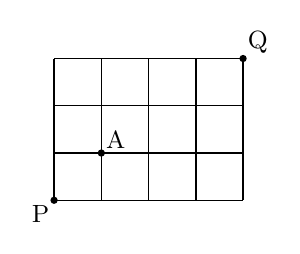
\begin{tikzpicture}[scale=0.6, line width=0.5pt]
  \draw[step=1] (0,0) grid (4,3);
  \fill (0,0) circle (2.2pt);
  \fill (4,3) circle (2.2pt);
  \fill (1,1) circle (2.2pt);
  \node[anchor=north east, inner sep=1.5pt, font=\small] at (0,0) {$\pt{P}$};
  \node[anchor=south west, inner sep=1.5pt, font=\small] at (4,3) {$\pt{Q}$};
  \node[anchor=south west, inner sep=1.5pt, font=\small] at (1,1) {$\pt{A}$};
\end{tikzpicture}
}\end{minipage}\par
\dmchoicesauto{\rule[-3ex]{0pt}{8ex}}{$\dfrac{3}{14}$}{$\dfrac{2}{7}$}{$\dfrac{5}{14}$}{$\dfrac{3}{7}$}{$\dfrac{1}{2}$}
}\vspace{8mm}
\setcounter{dmproblemcount}{11}\dmpnum{59-12}{% id: 59-12
% book: 베이직쎈 확률과 통계 · 03 확률의 뜻과 활용
% section: 실전 감각 UP
% figure: none
% answer: 
% answer_source: 
% variant_level: 0 (원본 전사)
% 이 파일은 build.mjs 가 items.json 에서 만든다. 고칠 때는 items.json 을 고친다.
\smash{\raisebox{1.5mm}{\dmkichul{베이직쎈 확률과 통계 59쪽 12번}}}
6개의 숫자 $1$, $2$, $3$, $4$, $5$, $6$에서 서로 다른 3개의 숫자를 뽑아 세 자리 자연수를 만들 때, 그 수가 $200$ 이상일 확률은?
\dmchoicesauto{\rule[-3ex]{0pt}{8ex}}{$\dfrac{3}{4}$}{$\dfrac{19}{24}$}{$\dfrac{5}{6}$}{$\dfrac{7}{8}$}{$\dfrac{11}{12}$}
}\vspace{8mm}
\setcounter{dmproblemcount}{12}\dmpnum{60-13}{% id: 60-13
% book: 베이직쎈 확률과 통계 · 03 확률의 뜻과 활용
% section: 실전 감각 UP
% figure: none
% answer: 
% answer_source: 
% variant_level: 0 (원본 전사)
% 이 파일은 build.mjs 가 items.json 에서 만든다. 고칠 때는 items.json 을 고친다.
\smash{\raisebox{1.5mm}{\dmkichul{베이직쎈 확률과 통계 60쪽 13번 · 서답형}}}
한 개의 주사위를 던지는 시행에서 소수의 눈이 나오는 사건을 $A$라 할 때, 사건 $A$와 배반인 사건의 개수를 구하시오.
}\vspace{8mm}
\setcounter{dmproblemcount}{13}\dmpnum{60-14}{% id: 60-14
% book: 베이직쎈 확률과 통계 · 03 확률의 뜻과 활용
% section: 실전 감각 UP
% figure: none
% answer: 
% answer_source: 
% variant_level: 0 (원본 전사)
% 이 파일은 build.mjs 가 items.json 에서 만든다. 고칠 때는 items.json 을 고친다.
\smash{\raisebox{1.5mm}{\dmkichul{베이직쎈 확률과 통계 60쪽 14번 · 서답형}}}
세 사람이 가위바위보를 한 번 할 때, 한 명이 이길 확률을 구하시오.
}\vspace{8mm}
\setcounter{dmproblemcount}{14}\dmpnum{60-15}{% id: 60-15
% book: 베이직쎈 확률과 통계 · 03 확률의 뜻과 활용
% section: 실전 감각 UP
% figure: tikz:fig-60-15
% answer: 
% answer_source: 
% variant_level: 0 (원본 전사)
% 이 파일은 build.mjs 가 items.json 에서 만든다. 고칠 때는 items.json 을 고친다.
\smash{\raisebox{1.5mm}{\dmkichul{베이직쎈 확률과 통계 60쪽 15번 · 서답형 · 서술형}}}
\noindent\begin{minipage}[t]{0.58\linewidth}\vspace{0pt}\raggedright 오른쪽 그림과 같이 평행한 두 직선 $l$, $m$ 위에 점이 각각 5개, 2개가 있다. 이 중에서 임의로 3개의 점을 택하여 선분으로 연결할 때, 삼각형이 만들어질 확률을 구하시오.\end{minipage}\hfill\begin{minipage}[t]{0.4\linewidth}\vspace{0pt}\centering \resizebox{\ifdim\width>\linewidth\linewidth\else\width\fi}{!}{% 60-15(인쇄 60쪽) — 평행한 두 직선 l, m 과 그 위의 점 5개·2개. 스캔 그림을 TikZ 로 다시 그림.
% 점에는 원문처럼 이름을 붙이지 않고, 라벨은 직선 이름 l·m 둘뿐이다(삼각형 개수 등 답의 근거는 적지 않는다).
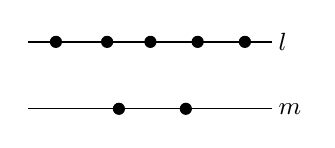
\begin{tikzpicture}[line width=0.5pt]
  \draw (0,0.85) -- (3.1,0.85);
  \foreach \x in {0.35,1.0,1.55,2.15,2.75} \fill (\x,0.85) circle (2.2pt);
  \node[anchor=west, inner sep=2pt, font=\small] at (3.1,0.85) {$l$};
  \draw (0,0) -- (3.1,0);
  \foreach \x in {1.15,2.0} \fill (\x,0) circle (2.2pt);
  \node[anchor=west, inner sep=2pt, font=\small] at (3.1,0) {$m$};
\end{tikzpicture}
}\end{minipage}\par
}\vspace{8mm}
\vspace{3mm}\setcounter{dmproblemcount}{15}\dmpnum{60-16}{% id: 60-16
% book: 베이직쎈 확률과 통계 · 03 확률의 뜻과 활용
% section: 실전 감각 UP
% figure: none
% answer: 
% answer_source: 
% variant_level: 0 (원본 전사)
% 이 파일은 build.mjs 가 items.json 에서 만든다. 고칠 때는 items.json 을 고친다.
\smash{\raisebox{4.5mm}{\dmkichul{베이직쎈 확률과 통계 60쪽 16번 · 서답형}}}
표본공간 $S$의 두 사건 $A$, $B$에 대하여 \par\smallskip\dispeq{$\mathrm{P}(A)=\dfrac{2}{3}$, $\mathrm{P}(B)=\dfrac{3}{4}$}\par\smallskip\noindent 일 때, $\mathrm{P}(A\cap B)$의 최솟값을 구하시오.
}\vspace{8mm}
\setcounter{dmproblemcount}{16}\dmpnum{60-17}{% id: 60-17
% book: 베이직쎈 확률과 통계 · 03 확률의 뜻과 활용
% section: 실전 감각 UP
% figure: none
% answer: 
% answer_source: 
% variant_level: 0 (원본 전사)
% 이 파일은 build.mjs 가 items.json 에서 만든다. 고칠 때는 items.json 을 고친다.
\smash{\raisebox{1.5mm}{\dmkichul{베이직쎈 확률과 통계 60쪽 17번 · 서답형}}}
$1$부터 $50$까지의 자연수가 각각 하나씩 적힌 50장의 카드가 들어 있는 상자에서 임의로 한 장의 카드를 꺼낼 때, $10$과 서로소인 수가 적힌 카드를 꺼낼 확률을 구하시오.
}\vspace{8mm}
\vspace{3mm}\setcounter{dmproblemcount}{17}\dmpnum{60-18}{% id: 60-18
% book: 베이직쎈 확률과 통계 · 03 확률의 뜻과 활용
% section: 실전 감각 UP
% figure: none
% answer: 
% answer_source: 
% variant_level: 0 (원본 전사)
% 이 파일은 build.mjs 가 items.json 에서 만든다. 고칠 때는 items.json 을 고친다.
\smash{\raisebox{4.5mm}{\dmkichul{베이직쎈 확률과 통계 60쪽 18번 · 서답형 · 서술형}}}
바구니에 서로 다른 8개의 떡이 들어 있는데 이 중 $n$개의 떡에는 꿀이 들어 있다. 이 바구니에서 임의로 2개의 떡을 동시에 꺼낼 때, 적어도 한 개의 떡에는 꿀이 들어 있을 확률이 $\dfrac{11}{14}$이다. 이때 $n$의 값을 구하시오. \dmcondfill{$1\le n\le 6$}{}
}\vspace{8mm}
\setcounter{dmproblemcount}{18}\dmpnum{60-19}{% id: 60-19
% book: 베이직쎈 확률과 통계 · 03 확률의 뜻과 활용
% section: 실전 감각 UP
% figure: none
% answer: 
% answer_source: 
% variant_level: 0 (원본 전사)
% 이 파일은 build.mjs 가 items.json 에서 만든다. 고칠 때는 items.json 을 고친다.
\smash{\raisebox{1.5mm}{\dmkichul{베이직쎈 확률과 통계 60쪽 19번 · 서답형 · 서술형 · 꼭 나와요}}}
노란색 팔찌 4개, 분홍색 팔찌 3개가 들어 있는 서랍에서 임의로 3개의 팔찌를 동시에 꺼낼 때, 노란색 팔찌를 2개 이하 꺼낼 확률을 구하시오.
}\vspace{8mm}
\vspace*{0pt plus 1filll}
\clearpage
\renewcommand{\dmchapunit}{04 조건부확률}
\dmchapter{04}{조건부확률}
\setcounter{dmproblemcount}{0}
\dmsection{개념 17 조건부확률}
\dmpassage{두 사건 $A$, $B$에 대하여\par\smallskip\centerline{$\mathrm{P}(A)=\dfrac{2}{3}$, $\mathrm{P}(B)=\dfrac{1}{2}$, $\mathrm{P}(A\cap B)=\dfrac{1}{4}$}\par\smallskip\noindent 일 때, 다음을 구하시오.}
\setcounter{dmproblemcount}{0}\dmpnum{62-01}{% id: 62-01
% book: 베이직쎈 확률과 통계 · 04 조건부확률
% section: 개념 17 조건부확률
% passage: 두 사건 $A$, $B$에 대하여\par\smallskip\centerline{$\mathrm{P}(A)=\dfrac{2}{3}$, $\mathrm{P}(B)=\dfrac{1}{2}$, $\mathrm{P}(A\cap B)=\dfrac{1}{4}$}\par\smallskip\noindent 일 때, 다음을 구하시오.
% figure: none
% answer: 
% answer_source: 
% variant_level: 0 (원본 전사)
% 이 파일은 build.mjs 가 items.json 에서 만든다. 고칠 때는 items.json 을 고친다.
\smash{\raisebox{1.5mm}{\dmkichul{베이직쎈 확률과 통계 62쪽 01번}}}
$\mathrm{P}(B\mid A)$
}\vspace{8mm}
\setcounter{dmproblemcount}{1}\dmpnum{62-02}{% id: 62-02
% book: 베이직쎈 확률과 통계 · 04 조건부확률
% section: 개념 17 조건부확률
% passage: 두 사건 $A$, $B$에 대하여\par\smallskip\centerline{$\mathrm{P}(A)=\dfrac{2}{3}$, $\mathrm{P}(B)=\dfrac{1}{2}$, $\mathrm{P}(A\cap B)=\dfrac{1}{4}$}\par\smallskip\noindent 일 때, 다음을 구하시오.
% figure: none
% answer: 
% answer_source: 
% variant_level: 0 (원본 전사)
% 이 파일은 build.mjs 가 items.json 에서 만든다. 고칠 때는 items.json 을 고친다.
\smash{\raisebox{1.5mm}{\dmkichul{베이직쎈 확률과 통계 62쪽 02번}}}
$\mathrm{P}(A\mid B)$
}\vspace{8mm}
\dmpassage{두 사건 $A$, $B$에 대하여\par\smallskip\centerline{$\mathrm{P}(A)=0.6$, $\mathrm{P}(B)=0.5$, $\mathrm{P}(A\cap B)=0.2$}\par\smallskip\noindent 일 때, 다음을 구하시오.}
\setcounter{dmproblemcount}{2}\dmpnum{62-03}{% id: 62-03
% book: 베이직쎈 확률과 통계 · 04 조건부확률
% section: 개념 17 조건부확률
% passage: 두 사건 $A$, $B$에 대하여\par\smallskip\centerline{$\mathrm{P}(A)=0.6$, $\mathrm{P}(B)=0.5$, $\mathrm{P}(A\cap B)=0.2$}\par\smallskip\noindent 일 때, 다음을 구하시오.
% figure: none
% answer: 
% answer_source: 
% variant_level: 0 (원본 전사)
% 이 파일은 build.mjs 가 items.json 에서 만든다. 고칠 때는 items.json 을 고친다.
\smash{\raisebox{1.5mm}{\dmkichul{베이직쎈 확률과 통계 62쪽 03번}}}
$\mathrm{P}(B\mid A)$
}\vspace{8mm}
\setcounter{dmproblemcount}{3}\dmpnum{62-04}{% id: 62-04
% book: 베이직쎈 확률과 통계 · 04 조건부확률
% section: 개념 17 조건부확률
% passage: 두 사건 $A$, $B$에 대하여\par\smallskip\centerline{$\mathrm{P}(A)=0.6$, $\mathrm{P}(B)=0.5$, $\mathrm{P}(A\cap B)=0.2$}\par\smallskip\noindent 일 때, 다음을 구하시오.
% figure: none
% answer: 
% answer_source: 
% variant_level: 0 (원본 전사)
% 이 파일은 build.mjs 가 items.json 에서 만든다. 고칠 때는 items.json 을 고친다.
\smash{\raisebox{1.5mm}{\dmkichul{베이직쎈 확률과 통계 62쪽 04번}}}
$\mathrm{P}(A\mid B)$
}\vspace{8mm}
\vspace{3mm}\setcounter{dmproblemcount}{4}\dmpnum{62-05}{% id: 62-05
% book: 베이직쎈 확률과 통계 · 04 조건부확률
% section: 개념 17 조건부확률
% figure: none
% answer: 
% answer_source: 
% variant_level: 0 (원본 전사)
% 이 파일은 build.mjs 가 items.json 에서 만든다. 고칠 때는 items.json 을 고친다.
\smash{\raisebox{4.5mm}{\dmkichul{베이직쎈 확률과 통계 62쪽 05번}}}
두 사건 $A$, $B$에 대하여\par\smallskip\dispeq{$\mathrm{P}(A)=\dfrac{1}{3}$, $\mathrm{P}(B)=\dfrac{3}{5}$, $\mathrm{P}(A\cup B)=\dfrac{13}{15}$}\par\smallskip\noindent 일 때, 다음을 구하시오.
\dmsubprob{1} $\mathrm{P}(A\cap B)$
\dmsubprob{2} $\mathrm{P}(B\mid A)$
}\vspace{8mm}
\dmpassage{두 사건 $A$, $B$에 대하여 다음을 구하시오.}
\vspace{3mm}\setcounter{dmproblemcount}{5}\dmpnum{62-06}{% id: 62-06
% book: 베이직쎈 확률과 통계 · 04 조건부확률
% section: 개념 17 조건부확률
% passage: 두 사건 $A$, $B$에 대하여 다음을 구하시오.
% figure: none
% answer: 
% answer_source: 
% variant_level: 0 (원본 전사)
% 이 파일은 build.mjs 가 items.json 에서 만든다. 고칠 때는 items.json 을 고친다.
\smash{\raisebox{4.5mm}{\dmkichul{베이직쎈 확률과 통계 62쪽 06번}}}
$\mathrm{P}(A)=\dfrac{3}{8}$, $\mathrm{P}(A\cap B)=\dfrac{1}{8}$, $\mathrm{P}(A\cup B)=\dfrac{3}{4}$일 때, $\mathrm{P}(A\mid B)$
}\vspace{8mm}
\setcounter{dmproblemcount}{6}\dmpnum{62-07}{% id: 62-07
% book: 베이직쎈 확률과 통계 · 04 조건부확률
% section: 개념 17 조건부확률
% passage: 두 사건 $A$, $B$에 대하여 다음을 구하시오.
% figure: none
% answer: 
% answer_source: 
% variant_level: 0 (원본 전사)
% 이 파일은 build.mjs 가 items.json 에서 만든다. 고칠 때는 items.json 을 고친다.
\smash{\raisebox{1.5mm}{\dmkichul{베이직쎈 확률과 통계 62쪽 07번}}}
$\mathrm{P}(B)=0.3$, $\mathrm{P}(A\cap B)=0.15$, $\mathrm{P}(A\cup B)=0.6$일 때, $\mathrm{P}(B\mid A)$
}\vspace{8mm}
\dmpassage{표본공간 $S$의 두 사건 $A$, $B$가 서로 배반사건일 때, 다음을 구하시오.}
\vspace{3mm}\setcounter{dmproblemcount}{7}\dmpnum{63-08}{% id: 63-08
% book: 베이직쎈 확률과 통계 · 04 조건부확률
% section: 개념 17 조건부확률
% passage: 표본공간 $S$의 두 사건 $A$, $B$가 서로 배반사건일 때, 다음을 구하시오.
% figure: none
% answer: 
% answer_source: 
% variant_level: 0 (원본 전사)
% 이 파일은 build.mjs 가 items.json 에서 만든다. 고칠 때는 items.json 을 고친다.
\smash{\raisebox{4.5mm}{\dmkichul{베이직쎈 확률과 통계 63쪽 08번}}}
$\mathrm{P}(A)=0.3$, $\mathrm{P}(B)=0.4$일 때,\par\smallskip\dispeq{$\mathrm{P}(B\mid \comp{A})=\dfrac{\mathrm{P}(B\cap \comp{A})}{\mathrm{P}(\comp{A})}=\dfrac{\mathrm{P}(B)-\mathrm{P}(A\cap B)}{\mathrm{P}(\comp{A})}$}\par\smallskip\dispeq{$=\dfrac{\mathrm{P}(\blank)}{\blank-\mathrm{P}(A)}=\dfrac{\blank}{0.7}=\blank$}\par
}\vspace{8mm}
\vspace{3mm}\setcounter{dmproblemcount}{8}\dmpnum{63-09}{% id: 63-09
% book: 베이직쎈 확률과 통계 · 04 조건부확률
% section: 개념 17 조건부확률
% passage: 표본공간 $S$의 두 사건 $A$, $B$가 서로 배반사건일 때, 다음을 구하시오.
% figure: none
% answer: 
% answer_source: 
% variant_level: 0 (원본 전사)
% 이 파일은 build.mjs 가 items.json 에서 만든다. 고칠 때는 items.json 을 고친다.
\smash{\raisebox{4.5mm}{\dmkichul{베이직쎈 확률과 통계 63쪽 09번}}}
$\mathrm{P}(A)=\dfrac{2}{5}$, $\mathrm{P}(B)=\dfrac{3}{10}$일 때, $\mathrm{P}(B\mid \comp{A})$
}\vspace{8mm}
\vspace{3mm}\setcounter{dmproblemcount}{9}\dmpnum{63-10}{% id: 63-10
% book: 베이직쎈 확률과 통계 · 04 조건부확률
% section: 개념 17 조건부확률
% passage: 표본공간 $S$의 두 사건 $A$, $B$가 서로 배반사건일 때, 다음을 구하시오.
% figure: none
% answer: 
% answer_source: 
% variant_level: 0 (원본 전사)
% 이 파일은 build.mjs 가 items.json 에서 만든다. 고칠 때는 items.json 을 고친다.
\smash{\raisebox{4.5mm}{\dmkichul{베이직쎈 확률과 통계 63쪽 10번}}}
$\mathrm{P}(A)=\dfrac{3}{7}$, $\mathrm{P}(B)=\dfrac{5}{14}$일 때, $\mathrm{P}(A\mid \comp{B})$
}\vspace{8mm}
\dmpassage{한 개의 주사위를 던지는 시행에서 나온 눈의 수가 2의 배수인 사건을 $A$, 3의 배수인 사건을 $B$라 할 때, 다음을 구하시오.}
\setcounter{dmproblemcount}{10}\dmpnum{63-11}{% id: 63-11
% book: 베이직쎈 확률과 통계 · 04 조건부확률
% section: 개념 17 조건부확률
% passage: 한 개의 주사위를 던지는 시행에서 나온 눈의 수가 2의 배수인 사건을 $A$, 3의 배수인 사건을 $B$라 할 때, 다음을 구하시오.
% figure: none
% answer: 
% answer_source: 
% variant_level: 0 (원본 전사)
% 이 파일은 build.mjs 가 items.json 에서 만든다. 고칠 때는 items.json 을 고친다.
\smash{\raisebox{1.5mm}{\dmkichul{베이직쎈 확률과 통계 63쪽 11번}}}
$\mathrm{P}(B\mid A)$
}\vspace{8mm}
\setcounter{dmproblemcount}{11}\dmpnum{63-12}{% id: 63-12
% book: 베이직쎈 확률과 통계 · 04 조건부확률
% section: 개념 17 조건부확률
% passage: 한 개의 주사위를 던지는 시행에서 나온 눈의 수가 2의 배수인 사건을 $A$, 3의 배수인 사건을 $B$라 할 때, 다음을 구하시오.
% figure: none
% answer: 
% answer_source: 
% variant_level: 0 (원본 전사)
% 이 파일은 build.mjs 가 items.json 에서 만든다. 고칠 때는 items.json 을 고친다.
\smash{\raisebox{1.5mm}{\dmkichul{베이직쎈 확률과 통계 63쪽 12번}}}
$\mathrm{P}(A\mid B)$
}\vspace{8mm}
\dmpassage{1부터 10까지의 자연수가 각각 하나씩 적힌 10장의 카드 중 임의로 한 장의 카드를 택하는 시행에서 택한 카드에 적힌 수가 홀수인 사건을 $A$, 소수인 사건을 $B$라 할 때, 다음을 구하시오.}
\setcounter{dmproblemcount}{12}\dmpnum{63-13}{% id: 63-13
% book: 베이직쎈 확률과 통계 · 04 조건부확률
% section: 개념 17 조건부확률
% passage: 1부터 10까지의 자연수가 각각 하나씩 적힌 10장의 카드 중 임의로 한 장의 카드를 택하는 시행에서 택한 카드에 적힌 수가 홀수인 사건을 $A$, 소수인 사건을 $B$라 할 때, 다음을 구하시오.
% figure: none
% answer: 
% answer_source: 
% variant_level: 0 (원본 전사)
% 이 파일은 build.mjs 가 items.json 에서 만든다. 고칠 때는 items.json 을 고친다.
\smash{\raisebox{1.5mm}{\dmkichul{베이직쎈 확률과 통계 63쪽 13번}}}
$\mathrm{P}(B\mid A)$
}\vspace{8mm}
\setcounter{dmproblemcount}{13}\dmpnum{63-14}{% id: 63-14
% book: 베이직쎈 확률과 통계 · 04 조건부확률
% section: 개념 17 조건부확률
% passage: 1부터 10까지의 자연수가 각각 하나씩 적힌 10장의 카드 중 임의로 한 장의 카드를 택하는 시행에서 택한 카드에 적힌 수가 홀수인 사건을 $A$, 소수인 사건을 $B$라 할 때, 다음을 구하시오.
% figure: none
% answer: 
% answer_source: 
% variant_level: 0 (원본 전사)
% 이 파일은 build.mjs 가 items.json 에서 만든다. 고칠 때는 items.json 을 고친다.
\smash{\raisebox{1.5mm}{\dmkichul{베이직쎈 확률과 통계 63쪽 14번}}}
$\mathrm{P}(A\mid B)$
}\vspace{8mm}
\dmpassage{한 개의 주사위를 던지는 시행에서 다음을 구하시오.}
\setcounter{dmproblemcount}{14}\dmpnum{63-15}{% id: 63-15
% book: 베이직쎈 확률과 통계 · 04 조건부확률
% section: 개념 17 조건부확률
% passage: 한 개의 주사위를 던지는 시행에서 다음을 구하시오.
% figure: none
% answer: 
% answer_source: 
% variant_level: 0 (원본 전사)
% 이 파일은 build.mjs 가 items.json 에서 만든다. 고칠 때는 items.json 을 고친다.
\smash{\raisebox{1.5mm}{\dmkichul{베이직쎈 확률과 통계 63쪽 15번}}}
짝수의 눈이 나왔을 때, 그 수가 5 이상일 확률
}\vspace{8mm}
\setcounter{dmproblemcount}{15}\dmpnum{63-16}{% id: 63-16
% book: 베이직쎈 확률과 통계 · 04 조건부확률
% section: 개념 17 조건부확률
% passage: 한 개의 주사위를 던지는 시행에서 다음을 구하시오.
% figure: none
% answer: 
% answer_source: 
% variant_level: 0 (원본 전사)
% 이 파일은 build.mjs 가 items.json 에서 만든다. 고칠 때는 items.json 을 고친다.
\smash{\raisebox{1.5mm}{\dmkichul{베이직쎈 확률과 통계 63쪽 16번}}}
3의 배수의 눈이 나왔을 때, 그 수가 홀수일 확률
}\vspace{8mm}
\setcounter{dmproblemcount}{16}\dmpnum{63-17}{% id: 63-17
% book: 베이직쎈 확률과 통계 · 04 조건부확률
% section: 개념 17 조건부확률
% passage: 한 개의 주사위를 던지는 시행에서 다음을 구하시오.
% figure: none
% answer: 
% answer_source: 
% variant_level: 0 (원본 전사)
% 이 파일은 build.mjs 가 items.json 에서 만든다. 고칠 때는 items.json 을 고친다.
\smash{\raisebox{1.5mm}{\dmkichul{베이직쎈 확률과 통계 63쪽 17번}}}
6의 약수의 눈이 나왔을 때, 그 수가 소수일 확률
}\vspace{8mm}
\dmpassage{다음을 구하시오.}
\setcounter{dmproblemcount}{17}\dmpnum{63-18}{% id: 63-18
% book: 베이직쎈 확률과 통계 · 04 조건부확률
% section: 개념 17 조건부확률
% passage: 다음을 구하시오.
% figure: none
% answer: 
% answer_source: 
% variant_level: 0 (원본 전사)
% 이 파일은 build.mjs 가 items.json 에서 만든다. 고칠 때는 items.json 을 고친다.
\smash{\raisebox{1.5mm}{\dmkichul{베이직쎈 확률과 통계 63쪽 18번}}}
서로 다른 두 개의 주사위를 동시에 던져서 나온 두 눈의 수가 같을 때, 그 두 수의 합이 10 이상일 확률
}\vspace{8mm}
\setcounter{dmproblemcount}{18}\dmpnum{63-19}{% id: 63-19
% book: 베이직쎈 확률과 통계 · 04 조건부확률
% section: 개념 17 조건부확률
% passage: 다음을 구하시오.
% figure: none
% answer: 
% answer_source: 
% variant_level: 0 (원본 전사)
% 이 파일은 build.mjs 가 items.json 에서 만든다. 고칠 때는 items.json 을 고친다.
\smash{\raisebox{1.5mm}{\dmkichul{베이직쎈 확률과 통계 63쪽 19번}}}
100원짜리 동전 1개, 50원짜리 동전 1개를 동시에 던져서 뒷면이 1개 나왔을 때, 뒷면이 나온 동전이 100원짜리 동전일 확률
}\vspace{8mm}
\setcounter{dmproblemcount}{19}\dmpnum{63-20}{% id: 63-20
% book: 베이직쎈 확률과 통계 · 04 조건부확률
% section: 개념 17 조건부확률
% passage: 다음을 구하시오.
% figure: none
% answer: 
% answer_source: 
% variant_level: 0 (원본 전사)
% 이 파일은 build.mjs 가 items.json 에서 만든다. 고칠 때는 items.json 을 고친다.
\smash{\raisebox{1.5mm}{\dmkichul{베이직쎈 확률과 통계 63쪽 20번}}}
1부터 12까지의 자연수가 각각 하나씩 적힌 12장의 카드 중 임의로 한 장의 카드를 택하는 시행에서 택한 카드에 적힌 수가 12의 약수일 때, 그 수가 홀수일 확률
}\vspace{8mm}
\dmsection{개념 18 확률의 곱셈정리}
\dmpassage{두 사건 $A$, $B$에 대하여\par\smallskip\centerline{$\mathrm{P}(A)=\dfrac{3}{4}$, $\mathrm{P}(B)=\dfrac{1}{2}$, $\mathrm{P}(B\mid A)=\dfrac{2}{5}$}\par\smallskip\noindent 일 때, 다음을 구하시오.}
\setcounter{dmproblemcount}{20}\dmpnum{64-21}{% id: 64-21
% book: 베이직쎈 확률과 통계 · 04 조건부확률
% section: 개념 18 확률의 곱셈정리
% passage: 두 사건 $A$, $B$에 대하여\par\smallskip\centerline{$\mathrm{P}(A)=\dfrac{3}{4}$, $\mathrm{P}(B)=\dfrac{1}{2}$, $\mathrm{P}(B\mid A)=\dfrac{2}{5}$}\par\smallskip\noindent 일 때, 다음을 구하시오.
% figure: none
% answer: 
% answer_source: 
% variant_level: 0 (원본 전사)
% 이 파일은 build.mjs 가 items.json 에서 만든다. 고칠 때는 items.json 을 고친다.
\smash{\raisebox{1.5mm}{\dmkichul{베이직쎈 확률과 통계 64쪽 21번}}}
$\mathrm{P}(A\cap B)$
}\vspace{8mm}
\setcounter{dmproblemcount}{21}\dmpnum{64-22}{% id: 64-22
% book: 베이직쎈 확률과 통계 · 04 조건부확률
% section: 개념 18 확률의 곱셈정리
% passage: 두 사건 $A$, $B$에 대하여\par\smallskip\centerline{$\mathrm{P}(A)=\dfrac{3}{4}$, $\mathrm{P}(B)=\dfrac{1}{2}$, $\mathrm{P}(B\mid A)=\dfrac{2}{5}$}\par\smallskip\noindent 일 때, 다음을 구하시오.
% figure: none
% answer: 
% answer_source: 
% variant_level: 0 (원본 전사)
% 이 파일은 build.mjs 가 items.json 에서 만든다. 고칠 때는 items.json 을 고친다.
\smash{\raisebox{1.5mm}{\dmkichul{베이직쎈 확률과 통계 64쪽 22번}}}
$\mathrm{P}(A\mid B)$
}\vspace{8mm}
\dmpassage{두 사건 $A$, $B$에 대하여 다음을 구하시오.}
\vspace{3mm}\setcounter{dmproblemcount}{22}\dmpnum{64-23}{% id: 64-23
% book: 베이직쎈 확률과 통계 · 04 조건부확률
% section: 개념 18 확률의 곱셈정리
% passage: 두 사건 $A$, $B$에 대하여 다음을 구하시오.
% figure: none
% answer: 
% answer_source: 
% variant_level: 0 (원본 전사)
% 이 파일은 build.mjs 가 items.json 에서 만든다. 고칠 때는 items.json 을 고친다.
\smash{\raisebox{4.5mm}{\dmkichul{베이직쎈 확률과 통계 64쪽 23번}}}
$\mathrm{P}(A)=\dfrac{1}{4}$, $\mathrm{P}(B)=\dfrac{3}{8}$, $\mathrm{P}(B\mid A)=\dfrac{1}{3}$일 때, $\mathrm{P}(A\mid B)$
}\vspace{8mm}
\setcounter{dmproblemcount}{23}\dmpnum{64-24}{% id: 64-24
% book: 베이직쎈 확률과 통계 · 04 조건부확률
% section: 개념 18 확률의 곱셈정리
% passage: 두 사건 $A$, $B$에 대하여 다음을 구하시오.
% figure: none
% answer: 
% answer_source: 
% variant_level: 0 (원본 전사)
% 이 파일은 build.mjs 가 items.json 에서 만든다. 고칠 때는 items.json 을 고친다.
\smash{\raisebox{1.5mm}{\dmkichul{베이직쎈 확률과 통계 64쪽 24번}}}
$\mathrm{P}(A)=0.7$, $\mathrm{P}(B)=0.5$, $\mathrm{P}(A\mid B)=0.6$일 때, $\mathrm{P}(B\mid A)$
}\vspace{8mm}
\vspace{3mm}\setcounter{dmproblemcount}{24}\dmpnum{64-25}{% id: 64-25
% book: 베이직쎈 확률과 통계 · 04 조건부확률
% section: 개념 18 확률의 곱셈정리
% passage: 두 사건 $A$, $B$에 대하여 다음을 구하시오.
% figure: none
% answer: 
% answer_source: 
% variant_level: 0 (원본 전사)
% 이 파일은 build.mjs 가 items.json 에서 만든다. 고칠 때는 items.json 을 고친다.
\smash{\raisebox{4.5mm}{\dmkichul{베이직쎈 확률과 통계 64쪽 25번}}}
$\mathrm{P}(\comp{A})=\dfrac{1}{6}$, $\mathrm{P}(B\mid A)=\dfrac{3}{4}$일 때, $\mathrm{P}(A\cap B)$
}\vspace{8mm}
\setcounter{dmproblemcount}{25}\dmpnum{64-26}{% id: 64-26
% book: 베이직쎈 확률과 통계 · 04 조건부확률
% section: 개념 18 확률의 곱셈정리
% figure: none
% answer: 
% answer_source: 
% variant_level: 0 (원본 전사)
% 이 파일은 build.mjs 가 items.json 에서 만든다. 고칠 때는 items.json 을 고친다.
\smash{\raisebox{1.5mm}{\dmkichul{베이직쎈 확률과 통계 64쪽 26번}}}
흰 구슬 2개, 검은 구슬 3개가 들어 있는 주머니에서 임의로 구슬을 한 개씩 두 번 꺼낼 때, 첫 번째에 흰 구슬을 꺼내는 사건을 $A$, 두 번째에 검은 구슬을 꺼내는 사건을 $B$라 하자. 다음을 구하시오. \dmcondfill{꺼낸 구슬은 다시 넣지 않는다.}{}
\dmsubprob{1} $\mathrm{P}(A)$
\dmsubprob{2} $\mathrm{P}(B\mid A)$
\dmsubprob{3} $\mathrm{P}(A\cap B)$
}\vspace{8mm}
\dmpassage{2개의 당첨 제비를 포함하여 7개의 제비가 들어 있는 상자에서 임의로 제비를 한 개씩 두 번 꺼낼 때, 다음을 구하시오. \cond{꺼낸 제비는 다시 넣지 않는다.}}
\setcounter{dmproblemcount}{26}\dmpnum{64-27}{% id: 64-27
% book: 베이직쎈 확률과 통계 · 04 조건부확률
% section: 개념 18 확률의 곱셈정리
% passage: 2개의 당첨 제비를 포함하여 7개의 제비가 들어 있는 상자에서 임의로 제비를 한 개씩 두 번 꺼낼 때, 다음을 구하시오. \cond{꺼낸 제비는 다시 넣지 않는다.}
% figure: none
% answer: 
% answer_source: 
% variant_level: 0 (원본 전사)
% 이 파일은 build.mjs 가 items.json 에서 만든다. 고칠 때는 items.json 을 고친다.
\smash{\raisebox{1.5mm}{\dmkichul{베이직쎈 확률과 통계 64쪽 27번}}}
두 번 모두 당첨 제비를 꺼낼 확률
}\vspace{8mm}
\setcounter{dmproblemcount}{27}\dmpnum{64-28}{% id: 64-28
% book: 베이직쎈 확률과 통계 · 04 조건부확률
% section: 개념 18 확률의 곱셈정리
% passage: 2개의 당첨 제비를 포함하여 7개의 제비가 들어 있는 상자에서 임의로 제비를 한 개씩 두 번 꺼낼 때, 다음을 구하시오. \cond{꺼낸 제비는 다시 넣지 않는다.}
% figure: none
% answer: 
% answer_source: 
% variant_level: 0 (원본 전사)
% 이 파일은 build.mjs 가 items.json 에서 만든다. 고칠 때는 items.json 을 고친다.
\smash{\raisebox{1.5mm}{\dmkichul{베이직쎈 확률과 통계 64쪽 28번}}}
첫 번째에만 당첨 제비를 꺼낼 확률
}\vspace{8mm}
\setcounter{dmproblemcount}{28}\dmpnum{64-29}{% id: 64-29
% book: 베이직쎈 확률과 통계 · 04 조건부확률
% section: 개념 18 확률의 곱셈정리
% passage: 2개의 당첨 제비를 포함하여 7개의 제비가 들어 있는 상자에서 임의로 제비를 한 개씩 두 번 꺼낼 때, 다음을 구하시오. \cond{꺼낸 제비는 다시 넣지 않는다.}
% figure: none
% answer: 
% answer_source: 
% variant_level: 0 (원본 전사)
% 이 파일은 build.mjs 가 items.json 에서 만든다. 고칠 때는 items.json 을 고친다.
\smash{\raisebox{1.5mm}{\dmkichul{베이직쎈 확률과 통계 64쪽 29번}}}
두 번째에만 당첨 제비를 꺼낼 확률
}\vspace{8mm}
\dmsection{개념 19 $\mathrm{P}(B)=\mathrm{P}(A\cap B)+\mathrm{P}(\comp{A}\cap B)$를 이용한 확률}
\setcounter{dmproblemcount}{29}\dmpnum{65-30}{% id: 65-30
% book: 베이직쎈 확률과 통계 · 04 조건부확률
% section: 개념 19 $\mathrm{P}(B)=\mathrm{P}(A\cap B)+\mathrm{P}(\comp{A}\cap B)$를 이용한 확률
% figure: none
% answer: 
% answer_source: 
% variant_level: 0 (원본 전사)
% 이 파일은 build.mjs 가 items.json 에서 만든다. 고칠 때는 items.json 을 고친다.
\smash{\raisebox{1.5mm}{\dmkichul{베이직쎈 확률과 통계 65쪽 30번}}}
2개의 당첨 제비를 포함하여 8개의 제비가 들어 있는 상자에서 임의로 제비를 한 개씩 두 번 뽑을 때, 첫 번째에 당첨 제비를 뽑는 사건을 $A$, 두 번째에 당첨 제비를 뽑는 사건을 $B$라 하자. 다음을 구하시오. \dmcondfill{뽑은 제비는 다시 넣지 않는다.}{}
\dmsubprob{1} 두 번 모두 당첨 제비를 뽑을 확률\dmhint{$\mathrm{P}(A\cap B)=\mathrm{P}(A)\mathrm{P}(\blank[3.2em])$\\ $\hphantom{\mathrm{P}(A\cap B)}=\dfrac{2}{8}\cdot\blank=\blank$}
\dmsubprob{2} 두 번째에만 당첨 제비를 뽑을 확률\dmhint{$\mathrm{P}(\comp{A}\cap B)=\mathrm{P}(\comp{A})\mathrm{P}(\blank[3.2em])$\\ $\hphantom{\mathrm{P}(\comp{A}\cap B)}=\dfrac{6}{8}\cdot\blank=\blank$}
\dmsubprob{3} 두 번째에 당첨 제비를 뽑을 확률\dmhint{두 사건 $A\cap B$와 $\comp{A}\cap B$는 서로 배반사건이므로\\ $\mathrm{P}(B)=\mathrm{P}(A\cap B)+\mathrm{P}(\blank[4em])$\\ $\hphantom{\mathrm{P}(B)}=\blank+\dfrac{3}{14}=\blank$}
}\vspace{8mm}
\setcounter{dmproblemcount}{30}\dmpnum{65-31}{% id: 65-31
% book: 베이직쎈 확률과 통계 · 04 조건부확률
% section: 개념 19 $\mathrm{P}(B)=\mathrm{P}(A\cap B)+\mathrm{P}(\comp{A}\cap B)$를 이용한 확률
% figure: none
% answer: 
% answer_source: 
% variant_level: 0 (원본 전사)
% 이 파일은 build.mjs 가 items.json 에서 만든다. 고칠 때는 items.json 을 고친다.
\smash{\raisebox{1.5mm}{\dmkichul{베이직쎈 확률과 통계 65쪽 31번}}}
빨간 구슬 4개, 노란 구슬 3개가 들어 있는 주머니에서 임의로 구슬을 한 개씩 두 번 꺼낼 때, 다음을 구하시오. \dmcondfill{꺼낸 구슬은 다시 넣지 않는다.}{}
\dmsubprob{1} 첫 번째에 빨간 구슬, 두 번째에 노란 구슬을 꺼낼 확률
\dmsubprob{2} 두 번 모두 노란 구슬을 꺼낼 확률
\dmsubprob{3} 두 번째에 노란 구슬을 꺼낼 확률
}\vspace{8mm}
\dmpassage{다음에 답하시오.}
\setcounter{dmproblemcount}{31}\dmpnum{66-32}{% id: 66-32
% book: 베이직쎈 확률과 통계 · 04 조건부확률
% section: 개념 19 $\mathrm{P}(B)=\mathrm{P}(A\cap B)+\mathrm{P}(\comp{A}\cap B)$를 이용한 확률
% passage: 다음에 답하시오.
% figure: none
% answer: 
% answer_source: 
% variant_level: 0 (원본 전사)
% 이 파일은 build.mjs 가 items.json 에서 만든다. 고칠 때는 items.json 을 고친다.
\smash{\raisebox{1.5mm}{\dmkichul{베이직쎈 확률과 통계 66쪽 32번}}}
4개의 불량품을 포함하여 12개의 제품이 들어 있는 상자에서 임의로 제품을 한 개씩 두 번 꺼낼 때, 두 번째에 불량품을 꺼낼 확률을 구하시오. \dmcondfill{꺼낸 제품은 다시 넣지 않는다.}{}
}\vspace{8mm}
\setcounter{dmproblemcount}{32}\dmpnum{66-33}{% id: 66-33
% book: 베이직쎈 확률과 통계 · 04 조건부확률
% section: 개념 19 $\mathrm{P}(B)=\mathrm{P}(A\cap B)+\mathrm{P}(\comp{A}\cap B)$를 이용한 확률
% passage: 다음에 답하시오.
% figure: none
% answer: 
% answer_source: 
% variant_level: 0 (원본 전사)
% 이 파일은 build.mjs 가 items.json 에서 만든다. 고칠 때는 items.json 을 고친다.
\smash{\raisebox{1.5mm}{\dmkichul{베이직쎈 확률과 통계 66쪽 33번}}}
흰 구슬 5개, 검은 구슬 4개가 들어 있는 주머니에서 임의로 구슬을 한 개씩 두 번 꺼낼 때, 두 번째에 흰 구슬을 꺼낼 확률을 구하시오. \dmcondfill{꺼낸 구슬은 다시 넣지 않는다.}{}
}\vspace{8mm}
\setcounter{dmproblemcount}{33}\dmpnum{66-34}{% id: 66-34
% book: 베이직쎈 확률과 통계 · 04 조건부확률
% section: 개념 19 $\mathrm{P}(B)=\mathrm{P}(A\cap B)+\mathrm{P}(\comp{A}\cap B)$를 이용한 확률
% passage: 다음에 답하시오.
% figure: none
% answer: 
% answer_source: 
% variant_level: 0 (원본 전사)
% 이 파일은 build.mjs 가 items.json 에서 만든다. 고칠 때는 items.json 을 고친다.
\smash{\raisebox{1.5mm}{\dmkichul{베이직쎈 확률과 통계 66쪽 34번}}}
3개의 당첨 제비를 포함한 10개의 제비 중에서 $\mathrm{A}$, $\mathrm{B}$ 두 사람이 이 순서대로 임의로 제비를 한 개씩 뽑을 때, $\mathrm{A}$가 당첨 제비를 뽑는 사건을 $A$, $\mathrm{B}$가 당첨 제비를 뽑는 사건을 $B$라 하자. 다음을 구하시오. \dmcondfill{뽑은 제비는 다시 넣지 않는다.}{}
\dmsubprob{1} $\mathrm{B}$가 당첨 제비를 뽑을 확률\dmhint{$\mathrm{P}(B)=\mathrm{P}(A\cap B)+\mathrm{P}(\blank[4em])$\\ $\hphantom{\mathrm{P}(B)}=\mathrm{P}(A)\mathrm{P}(\blank[3.2em])+\mathrm{P}(\comp{A})\mathrm{P}(B\mid \comp{A})$\\ $\hphantom{\mathrm{P}(B)}=\dfrac{3}{10}\cdot\blank+\blank\cdot\dfrac{3}{9}=\blank$}
\dmsubprob{2} $\mathrm{B}$가 당첨 제비를 뽑았을 때, $\mathrm{A}$가 당첨 제비를 뽑았을 확률\dmhint{$\mathrm{P}(A\mid B)=\dfrac{\mathrm{P}(\blank[4em])}{\mathrm{P}(B)}=\dfrac{\blank}{\blank}=\blank$}
}\vspace{8mm}
\setcounter{dmproblemcount}{34}\dmpnum{66-35}{% id: 66-35
% book: 베이직쎈 확률과 통계 · 04 조건부확률
% section: 개념 19 $\mathrm{P}(B)=\mathrm{P}(A\cap B)+\mathrm{P}(\comp{A}\cap B)$를 이용한 확률
% passage: 다음에 답하시오.
% figure: none
% answer: 
% answer_source: 
% variant_level: 0 (원본 전사)
% 이 파일은 build.mjs 가 items.json 에서 만든다. 고칠 때는 items.json 을 고친다.
\smash{\raisebox{1.5mm}{\dmkichul{베이직쎈 확률과 통계 66쪽 35번}}}
노란 공 4개, 검은 공 6개가 들어 있는 $\mathrm{A}$ 주머니와 노란 공 2개, 검은 공 4개가 들어 있는 $\mathrm{B}$ 주머니 중 임의로 하나를 택하여 한 개의 공을 꺼낼 때, $\mathrm{A}$ 주머니를 택하는 사건을 $A$, $\mathrm{B}$ 주머니를 택하는 사건을 $B$, 꺼낸 공이 검은 공인 사건을 $E$라 하자. 다음을 구하시오.
\dmsubprob{1} 꺼낸 공이 검은 공일 확률\dmhint{$\mathrm{P}(A)=\dfrac{1}{2}$, $\mathrm{P}(B)=\blank$이므로\\ $\mathrm{P}(E)=\mathrm{P}(A\cap E)+\mathrm{P}(\blank[4em])$\\ $\hphantom{\mathrm{P}(E)}=\mathrm{P}(A)\mathrm{P}(E\mid A)+\mathrm{P}(B)\mathrm{P}(\blank[3.2em])$\\ $\hphantom{\mathrm{P}(E)}=\dfrac{1}{2}\cdot\dfrac{\blank}{10}+\dfrac{1}{2}\cdot\dfrac{\blank}{6}=\blank$}
\dmsubprob{2} 꺼낸 공이 검은 공일 때, 택한 주머니가 $\mathrm{A}$일 확률\dmhint{$\mathrm{P}(A\mid E)=\dfrac{\mathrm{P}(A\cap E)}{\mathrm{P}(\blank)}=\dfrac{\blank}{\blank}=\blank$}
}\vspace{8mm}
\setcounter{dmproblemcount}{35}\dmpnum{66-36}{% id: 66-36
% book: 베이직쎈 확률과 통계 · 04 조건부확률
% section: 개념 19 $\mathrm{P}(B)=\mathrm{P}(A\cap B)+\mathrm{P}(\comp{A}\cap B)$를 이용한 확률
% passage: 다음에 답하시오.
% figure: none
% answer: 
% answer_source: 
% variant_level: 0 (원본 전사)
% 이 파일은 build.mjs 가 items.json 에서 만든다. 고칠 때는 items.json 을 고친다.
\smash{\raisebox{1.5mm}{\dmkichul{베이직쎈 확률과 통계 66쪽 36번}}}
빨간 구슬 6개, 파란 구슬 7개가 들어 있는 상자에서 $\mathrm{A}$, $\mathrm{B}$ 두 사람이 이 순서대로 임의로 구슬을 한 개씩 꺼낸다. $\mathrm{B}$가 빨간 구슬을 꺼냈을 때, $\mathrm{A}$가 파란 구슬을 꺼냈을 확률을 구하시오. \dmcondfill{꺼낸 구슬은 다시 넣지 않는다.}{}
}\vspace{8mm}
\setcounter{dmproblemcount}{36}\dmpnum{66-37}{% id: 66-37
% book: 베이직쎈 확률과 통계 · 04 조건부확률
% section: 개념 19 $\mathrm{P}(B)=\mathrm{P}(A\cap B)+\mathrm{P}(\comp{A}\cap B)$를 이용한 확률
% passage: 다음에 답하시오.
% figure: none
% answer: 
% answer_source: 
% variant_level: 0 (원본 전사)
% 이 파일은 build.mjs 가 items.json 에서 만든다. 고칠 때는 items.json 을 고친다.
\smash{\raisebox{1.5mm}{\dmkichul{베이직쎈 확률과 통계 66쪽 37번}}}
꿀이 들어 있는 송편 2개를 포함하여 7개의 송편이 담겨 있는 $\mathrm{A}$ 접시와 꿀이 들어 있는 송편 2개를 포함하여 6개의 송편이 담겨 있는 $\mathrm{B}$ 접시가 있다. 두 접시 $\mathrm{A}$, $\mathrm{B}$ 중 임의로 하나를 택하여 한 개의 송편을 먹었더니 꿀이 들어 있는 송편이었을 때, 택한 접시가 $\mathrm{B}$일 확률을 구하시오.
}\vspace{8mm}
\dmsection{유형 037 조건부확률의 계산}
\vspace{3mm}\setcounter{dmproblemcount}{0}\dmpnum{67-01}{% id: 67-01
% book: 베이직쎈 확률과 통계 · 04 조건부확률
% section: 유형 037 조건부확률의 계산
% figure: none
% answer: 
% answer_source: 
% variant_level: 0 (원본 전사)
% 이 파일은 build.mjs 가 items.json 에서 만든다. 고칠 때는 items.json 을 고친다.
\smash{\raisebox{4.5mm}{\dmkichul{베이직쎈 확률과 통계 67쪽 01번}}}
두 사건 $A$, $B$에 대하여\par\smallskip\dispeq{$\mathrm{P}(\comp{B})=\dfrac{2}{5}$, $\mathrm{P}(A\cap B)=\dfrac{3}{20}$}\par\smallskip\noindent 일 때, $\mathrm{P}(A\mid B)$를 구하시오.
}\vspace{8mm}
\vspace{3mm}\setcounter{dmproblemcount}{1}\dmpnum{67-02}{% id: 67-02
% book: 베이직쎈 확률과 통계 · 04 조건부확률
% section: 유형 037 조건부확률의 계산
% figure: none
% answer: 
% answer_source: 
% variant_level: 0 (원본 전사)
% 이 파일은 build.mjs 가 items.json 에서 만든다. 고칠 때는 items.json 을 고친다.
\smash{\raisebox{4.5mm}{\dmkichul{베이직쎈 확률과 통계 67쪽 02번}}}
두 사건 $A$, $B$에 대하여\par\smallskip\dispeq{$\mathrm{P}(A)=\dfrac{3}{4}$, $\mathrm{P}(A\cap\comp{B})=\dfrac{5}{12}$}\par\smallskip\noindent 일 때, $\mathrm{P}(B\mid A)$는?
\dmchoicesauto{\rule[-3ex]{0pt}{8ex}}{$\dfrac{1}{9}$}{$\dfrac{2}{9}$}{$\dfrac{1}{3}$}{$\dfrac{4}{9}$}{$\dfrac{5}{9}$}
}\vspace{8mm}
\setcounter{dmproblemcount}{2}\dmpnum{67-03}{% id: 67-03
% book: 베이직쎈 확률과 통계 · 04 조건부확률
% section: 유형 037 조건부확률의 계산
% figure: none
% answer: 
% answer_source: 
% variant_level: 0 (원본 전사)
% 이 파일은 build.mjs 가 items.json 에서 만든다. 고칠 때는 items.json 을 고친다.
\smash{\raisebox{1.5mm}{\dmkichul{베이직쎈 확률과 통계 67쪽 03번}}}
두 사건 $A$, $B$에 대하여\par\smallskip\dispeq{$\mathrm{P}(A)=0.45$, $\mathrm{P}(B)=0.3$, $\mathrm{P}(\comp{A}\cap\comp{B})=0.3$}\par\smallskip\noindent 일 때, $\mathrm{P}(A\mid B)$를 구하시오.
}\vspace{8mm}
\setcounter{dmproblemcount}{3}\dmpnum{67-04}{% id: 67-04
% book: 베이직쎈 확률과 통계 · 04 조건부확률
% section: 유형 037 조건부확률의 계산
% figure: none
% answer: 
% answer_source: 
% variant_level: 0 (원본 전사)
% 이 파일은 build.mjs 가 items.json 에서 만든다. 고칠 때는 items.json 을 고친다.
\smash{\raisebox{1.5mm}{\dmkichul{베이직쎈 확률과 통계 67쪽 04번}}}
두 사건 $A$, $B$에 대하여\par\smallskip\dispeq{$\mathrm{P}(A)=0.55$, $\mathrm{P}(A\mid B)=0.5$, $\mathrm{P}(A\cup B)=0.7$}\par\smallskip\noindent 일 때, $\mathrm{P}(A\cap B)$를 구하시오.
}\vspace{8mm}
\vspace{3mm}\setcounter{dmproblemcount}{4}\dmpnum{67-05}{% id: 67-05
% book: 베이직쎈 확률과 통계 · 04 조건부확률
% section: 유형 037 조건부확률의 계산
% figure: none
% answer: 
% answer_source: 
% variant_level: 0 (원본 전사)
% 이 파일은 build.mjs 가 items.json 에서 만든다. 고칠 때는 items.json 을 고친다.
\smash{\raisebox{4.5mm}{\dmkichul{베이직쎈 확률과 통계 67쪽 05번}}}
두 사건 $A$, $B$에 대하여\par\smallskip\dispeq{$\mathrm{P}(\comp{A})=\dfrac{1}{3}$, $\mathrm{P}(B\mid A)=\dfrac{1}{2}$, $\mathrm{P}(A\mid B)=\dfrac{5}{6}$}\par\smallskip\noindent 일 때, $\mathrm{P}(B)$는?
\dmchoicesauto{\rule[-3ex]{0pt}{8ex}}{$\dfrac{1}{10}$}{$\dfrac{1}{5}$}{$\dfrac{3}{10}$}{$\dfrac{2}{5}$}{$\dfrac{1}{2}$}
}\vspace{8mm}
\vspace{3mm}\setcounter{dmproblemcount}{5}\dmpnum{67-06}{% id: 67-06
% book: 베이직쎈 확률과 통계 · 04 조건부확률
% section: 유형 037 조건부확률의 계산
% figure: none
% answer: 
% answer_source: 
% variant_level: 0 (원본 전사)
% 이 파일은 build.mjs 가 items.json 에서 만든다. 고칠 때는 items.json 을 고친다.
\smash{\raisebox{4.5mm}{\dmkichul{베이직쎈 확률과 통계 67쪽 06번}}}
두 사건 $A$, $B$가 서로 배반사건이고\par\smallskip\dispeq{$\mathrm{P}(A)=\dfrac{1}{4}$, $\mathrm{P}(B)=\dfrac{3}{5}$}\par\smallskip\noindent 일 때, $\mathrm{P}(B\mid\comp{A})$는?
\dmchoicesauto{\rule[-3ex]{0pt}{8ex}}{$\dfrac{3}{5}$}{$\dfrac{13}{20}$}{$\dfrac{7}{10}$}{$\dfrac{3}{4}$}{$\dfrac{4}{5}$}
}\vspace{8mm}
\dmsection{유형 038 조건부확률}
\setcounter{dmproblemcount}{6}\dmpnum{68-07}{% id: 68-07
% book: 베이직쎈 확률과 통계 · 04 조건부확률
% section: 유형 038 조건부확률
% figure: none
% answer: 
% answer_source: 
% variant_level: 0 (원본 전사)
% 이 파일은 build.mjs 가 items.json 에서 만든다. 고칠 때는 items.json 을 고친다.
\smash{\raisebox{1.5mm}{\dmkichul{베이직쎈 확률과 통계 68쪽 07번}}}
한 개의 동전을 두 번 던져서 앞면이 한 번 나왔을 때, 첫 번째에 앞면이 나왔을 확률은?
\dmchoicesauto{\rule[-3ex]{0pt}{8ex}}{$\dfrac{1}{8}$}{$\dfrac{1}{4}$}{$\dfrac{3}{8}$}{$\dfrac{1}{2}$}{$\dfrac{5}{8}$}
}\vspace{8mm}
\vspace{3mm}\setcounter{dmproblemcount}{7}\dmpnum{68-08}{% id: 68-08
% book: 베이직쎈 확률과 통계 · 04 조건부확률
% section: 유형 038 조건부확률
% figure: none
% answer: 
% answer_source: 
% variant_level: 0 (원본 전사)
% 이 파일은 build.mjs 가 items.json 에서 만든다. 고칠 때는 items.json 을 고친다.
\smash{\raisebox{4.5mm}{\dmkichul{베이직쎈 확률과 통계 68쪽 08번}}}
어느 학급에서 피아노를 배운 적이 있는 학생은 전체 학생의 $\dfrac{5}{8}$이고, 피아노를 배운 적이 있는 여학생은 전체 학생의 $\dfrac{3}{16}$이다. 이 학급 전체 학생 중 임의로 택한 한 명이 피아노를 배운 적이 있을 때, 그 학생이 여학생일 확률을 구하시오.
}\vspace{8mm}
\setcounter{dmproblemcount}{8}\dmpnum{68-09}{% id: 68-09
% book: 베이직쎈 확률과 통계 · 04 조건부확률
% section: 유형 038 조건부확률
% figure: none
% answer: 
% answer_source: 
% variant_level: 0 (원본 전사)
% 이 파일은 build.mjs 가 items.json 에서 만든다. 고칠 때는 items.json 을 고친다.
\smash{\raisebox{1.5mm}{\dmkichul{베이직쎈 확률과 통계 68쪽 09번}}}
어느 날에 놀이공원을 찾은 전체 이용객의 $54\mkern3mu \%$는 어린이이고, 남자 어린이는 전체 이용객의 $30\mkern3mu \%$이다. 이 날 놀이공원을 찾은 전체 이용객 중 임의로 택한 한 명이 어린이일 때, 그 어린이가 남자일 확률을 구하시오.
}\vspace{8mm}
\setcounter{dmproblemcount}{9}\dmpnum{68-10}{% id: 68-10
% book: 베이직쎈 확률과 통계 · 04 조건부확률
% section: 유형 038 조건부확률
% figure: none
% answer: 
% answer_source: 
% variant_level: 0 (원본 전사)
% 이 파일은 build.mjs 가 items.json 에서 만든다. 고칠 때는 items.json 을 고친다.
\smash{\raisebox{1.5mm}{\dmkichul{베이직쎈 확률과 통계 68쪽 10번}}}
서로 다른 두 개의 주사위를 동시에 던져서 나온 두 눈의 수의 곱이 20 이상일 때, 그 두 수의 차가 2일 확률을 구하시오.
}\vspace{8mm}
\setcounter{dmproblemcount}{10}\dmpnum{68-11}{% id: 68-11
% book: 베이직쎈 확률과 통계 · 04 조건부확률
% section: 유형 038 조건부확률
% figure: none
% answer: 
% answer_source: 
% variant_level: 0 (원본 전사)
% 이 파일은 build.mjs 가 items.json 에서 만든다. 고칠 때는 items.json 을 고친다.
\smash{\raisebox{1.5mm}{\dmkichul{베이직쎈 확률과 통계 68쪽 11번}}}
1, 2, 3, 4가 각각 하나씩 적힌 흰색 카드 4장과 6, 7, 8, 9, 10이 각각 하나씩 적힌 검은색 카드 5장이 들어 있는 상자가 있다. 이 상자에서 임의로 꺼낸 한 장의 카드가 검은색일 때, 그 카드에 적힌 숫자가 짝수일 확률은?
\dmchoicesauto{\rule[-3ex]{0pt}{8ex}}{$\dfrac{1}{5}$}{$\dfrac{3}{10}$}{$\dfrac{2}{5}$}{$\dfrac{1}{2}$}{$\dfrac{3}{5}$}
}\vspace{8mm}
\setcounter{dmproblemcount}{11}\dmpnum{68-12}{% id: 68-12
% book: 베이직쎈 확률과 통계 · 04 조건부확률
% section: 유형 038 조건부확률
% figure: none
% answer: 
% answer_source: 
% variant_level: 0 (원본 전사)
% 이 파일은 build.mjs 가 items.json 에서 만든다. 고칠 때는 items.json 을 고친다.
\smash{\raisebox{1.5mm}{\dmkichul{베이직쎈 확률과 통계 68쪽 12번}}}
불량품 1개를 포함한 P 회사의 제품 10개와 불량품 2개를 포함한 Q 회사의 제품 10개가 있다. 이 20개의 제품 중 임의로 택한 한 개의 제품이 불량품일 때, 그 불량품이 Q 회사의 제품일 확률은?
\dmchoicesauto{\rule[-3ex]{0pt}{8ex}}{$\dfrac{3}{5}$}{$\dfrac{2}{3}$}{$\dfrac{11}{15}$}{$\dfrac{4}{5}$}{$\dfrac{13}{15}$}
}\vspace{8mm}
\dmsection{유형 039 표를 이용한 조건부확률}
\setcounter{dmproblemcount}{12}\dmpnum{69-13}{% id: 69-13
% book: 베이직쎈 확률과 통계 · 04 조건부확률
% section: 유형 039 표를 이용한 조건부확률
% figure: none
% answer: 
% answer_source: 
% variant_level: 0 (원본 전사)
% 이 파일은 build.mjs 가 items.json 에서 만든다. 고칠 때는 items.json 을 고친다.
\smash{\raisebox{1.5mm}{\dmkichul{베이직쎈 확률과 통계 69쪽 13번}}}
아래는 어느 고등학교 1학년 학생 100명을 대상으로 등교할 때 자전거를 이용하는지 조사하여 나타낸 표이다. 조사 대상 학생 중 임의로 한 명을 택할 때, 다음을 구하시오.\par\noindent\hfill{\footnotesize (단위: 명)}\par\smallskip\dispeq{\begin{tabular}{|c|c|c|c|}\hline & 남학생 & 여학생 & 합계 \\ \hline 자전거 이용 & 24 & 16 & 40 \\ \hline 자전거 이용 안 함 & 30 & 30 & 60 \\ \hline 합계 & 54 & 46 & 100 \\ \hline\end{tabular}}\par\smallskip\noindent
\dmsubprob{1} 택한 학생이 자전거를 이용할 때, 그 학생이 남학생일 확률
\dmsubprob{2} 택한 학생이 남학생일 때, 그 학생이 자전거를 이용할 확률
}\vspace{8mm}
\setcounter{dmproblemcount}{13}\dmpnum{69-14}{% id: 69-14
% book: 베이직쎈 확률과 통계 · 04 조건부확률
% section: 유형 039 표를 이용한 조건부확률
% figure: none
% answer: 
% answer_source: 
% variant_level: 0 (원본 전사)
% 이 파일은 build.mjs 가 items.json 에서 만든다. 고칠 때는 items.json 을 고친다.
\smash{\raisebox{1.5mm}{\dmkichul{베이직쎈 확률과 통계 69쪽 14번}}}
아래는 어느 고등학교 학생 50명을 대상으로 정기적으로 봉사 활동을 하고 있는지 조사하여 나타낸 표이다. 조사 대상 학생 중 임의로 택한 한 명이 여학생일 때, 그 학생이 정기적으로 봉사 활동을 하는 학생일 확률을 구하시오.\par\noindent\hfill{\footnotesize (단위: 명)}\par\smallskip\dispeq{\begin{tabular}{|c|c|c|c|}\hline & 남학생 & 여학생 & 합계 \\ \hline 봉사 활동을 하고 있음 & 10 & & 22 \\ \hline 봉사 활동을 하고 있지 않음 & & 13 & \\ \hline 합계 & & & 50 \\ \hline\end{tabular}}\par\smallskip\noindent
}\vspace{8mm}
\setcounter{dmproblemcount}{14}\dmpnum{69-15}{% id: 69-15
% book: 베이직쎈 확률과 통계 · 04 조건부확률
% section: 유형 039 표를 이용한 조건부확률
% figure: none
% answer: 
% answer_source: 
% variant_level: 0 (원본 전사)
% 이 파일은 build.mjs 가 items.json 에서 만든다. 고칠 때는 items.json 을 고친다.
\smash{\raisebox{1.5mm}{\dmkichul{베이직쎈 확률과 통계 69쪽 15번}}}
두 야구 동호회 P, Q의 투수는 각각 14명, 16명이다. P 동호회의 투수 중 공을 던질 때 오른손만 사용하는 회원은 8명, 왼손만 사용하는 회원은 6명이고, Q 동호회의 투수 중 공을 던질 때 오른손만 사용하는 회원은 12명, 왼손만 사용하는 회원은 4명이다. 두 동호회의 투수 중 임의로 택한 한 명이 왼손만 사용하는 회원일 때, 그 회원이 Q 동호회 회원일 확률은?
\dmchoicesauto{\rule[-3ex]{0pt}{8ex}}{$\dfrac{3}{10}$}{$\dfrac{2}{5}$}{$\dfrac{1}{2}$}{$\dfrac{3}{5}$}{$\dfrac{7}{10}$}
}\vspace{8mm}
\setcounter{dmproblemcount}{15}\dmpnum{69-16}{% id: 69-16
% book: 베이직쎈 확률과 통계 · 04 조건부확률
% section: 유형 039 표를 이용한 조건부확률
% figure: none
% answer: 
% answer_source: 
% variant_level: 0 (원본 전사)
% 이 파일은 build.mjs 가 items.json 에서 만든다. 고칠 때는 items.json 을 고친다.
\smash{\raisebox{1.5mm}{\dmkichul{베이직쎈 확률과 통계 69쪽 16번}}}
어느 지역의 남학생 80명, 여학생 40명을 대상으로 조사하였더니 남학생 20명과 여학생 15명이 손목시계를 차고 있었다. 조사 대상 학생 중 임의로 택한 한 명이 손목시계를 차고 있지 않을 때, 그 학생이 남학생일 확률은?
\dmchoicesauto{\rule[-3ex]{0pt}{8ex}}{$\dfrac{9}{17}$}{$\dfrac{10}{17}$}{$\dfrac{11}{17}$}{$\dfrac{12}{17}$}{$\dfrac{13}{17}$}
}\vspace{8mm}
\setcounter{dmproblemcount}{16}\dmpnum{69-17}{% id: 69-17
% book: 베이직쎈 확률과 통계 · 04 조건부확률
% section: 유형 039 표를 이용한 조건부확률
% figure: none
% answer: 
% answer_source: 
% variant_level: 0 (원본 전사)
% 이 파일은 build.mjs 가 items.json 에서 만든다. 고칠 때는 items.json 을 고친다.
\smash{\raisebox{1.5mm}{\dmkichul{베이직쎈 확률과 통계 69쪽 17번}}}
남학생 18명과 여학생 17명으로 구성된 어느 영화 동아리의 모든 학생들이 두 영화 P, Q 중 하나를 택하여 관람하였다. 남학생 중에서 P 영화를 관람한 학생은 10명이고, 여학생 중에서 Q 영화를 관람한 학생은 11명이다. 이 동아리에서 임의로 택한 한 명이 P 영화를 관람하였을 때, 그 학생이 여학생일 확률을 구하시오.
}\vspace{8mm}
\dmsection{유형 040 확률의 곱셈정리}
\setcounter{dmproblemcount}{17}\dmpnum{70-18}{% id: 70-18
% book: 베이직쎈 확률과 통계 · 04 조건부확률
% section: 유형 040 확률의 곱셈정리
% figure: none
% answer: 
% answer_source: 
% variant_level: 0 (원본 전사)
% 이 파일은 build.mjs 가 items.json 에서 만든다. 고칠 때는 items.json 을 고친다.
\smash{\raisebox{1.5mm}{\dmkichul{베이직쎈 확률과 통계 70쪽 18번}}}
4개의 당첨 제비를 포함한 10개의 제비 중에서 은영, 주호 두 사람이 이 순서대로 임의로 제비를 한 개씩 뽑을 때, 두 사람 모두 당첨 제비를 뽑을 확률은? \dmcondfill{뽑은 제비는 다시 넣지 않는다.}{}
\dmchoicesauto{\rule[-3ex]{0pt}{8ex}}{$\dfrac{1}{15}$}{$\dfrac{2}{15}$}{$\dfrac{1}{5}$}{$\dfrac{4}{15}$}{$\dfrac{1}{3}$}
}\vspace{8mm}
\setcounter{dmproblemcount}{18}\dmpnum{70-19}{% id: 70-19
% book: 베이직쎈 확률과 통계 · 04 조건부확률
% section: 유형 040 확률의 곱셈정리
% figure: none
% answer: 
% answer_source: 
% variant_level: 0 (원본 전사)
% 이 파일은 build.mjs 가 items.json 에서 만든다. 고칠 때는 items.json 을 고친다.
\smash{\raisebox{1.5mm}{\dmkichul{베이직쎈 확률과 통계 70쪽 19번}}}
남자 회원이 9명, 여자 회원이 6명인 어느 사진 동호회에서 대표 2명을 뽑으려고 한다. 임의로 한 명씩 차례대로 뽑을 때, 첫 번째에 남자 회원, 두 번째에 여자 회원을 뽑을 확률을 구하시오.
}\vspace{8mm}
\setcounter{dmproblemcount}{19}\dmpnum{70-20}{% id: 70-20
% book: 베이직쎈 확률과 통계 · 04 조건부확률
% section: 유형 040 확률의 곱셈정리
% figure: none
% answer: 
% answer_source: 
% variant_level: 0 (원본 전사)
% 이 파일은 build.mjs 가 items.json 에서 만든다. 고칠 때는 items.json 을 고친다.
\smash{\raisebox{1.5mm}{\dmkichul{베이직쎈 확률과 통계 70쪽 20번}}}
파란 공 8개와 흰 공 4개가 들어 있는 주머니에서 임의로 공을 한 개씩 두 번 꺼낼 때, 두 번째에만 흰 공을 꺼낼 확률을 구하시오. \dmcondfill{꺼낸 공은 다시 넣지 않는다.}{}
}\vspace{8mm}
\setcounter{dmproblemcount}{20}\dmpnum{70-21}{% id: 70-21
% book: 베이직쎈 확률과 통계 · 04 조건부확률
% section: 유형 040 확률의 곱셈정리
% figure: none
% answer: 
% answer_source: 
% variant_level: 0 (원본 전사)
% 이 파일은 build.mjs 가 items.json 에서 만든다. 고칠 때는 items.json 을 고친다.
\smash{\raisebox{1.5mm}{\dmkichul{베이직쎈 확률과 통계 70쪽 21번}}}
1부터 15까지의 자연수가 각각 하나씩 적힌 15장의 카드가 들어 있는 상자에서 임의로 카드를 한 장씩 두 번 꺼낼 때, 두 번 모두 14의 약수가 적힌 카드를 꺼낼 확률은? \dmcondfill{꺼낸 카드는 다시 넣지 않는다.}{}
\dmchoicesauto{\rule[-3ex]{0pt}{8ex}}{$\dfrac{1}{35}$}{$\dfrac{2}{35}$}{$\dfrac{3}{35}$}{$\dfrac{4}{35}$}{$\dfrac{1}{7}$}
}\vspace{8mm}
\vspace{3mm}\setcounter{dmproblemcount}{21}\dmpnum{70-22}{% id: 70-22
% book: 베이직쎈 확률과 통계 · 04 조건부확률
% section: 유형 040 확률의 곱셈정리
% figure: none
% answer: 
% answer_source: 
% variant_level: 0 (원본 전사)
% 이 파일은 build.mjs 가 items.json 에서 만든다. 고칠 때는 items.json 을 고친다.
\smash{\raisebox{4.5mm}{\dmkichul{베이직쎈 확률과 통계 70쪽 22번}}}
성훈이가 아침 식사로 빵을 먹을 확률은 $\dfrac{1}{4}$이고, 아침 식사로 빵을 먹지 않았을 때 점심 식사로 빵을 먹지 않을 확률은 $\dfrac{1}{2}$이다. 성훈이가 아침 식사, 점심 식사로 모두 빵을 먹지 않을 확률을 구하시오.
}\vspace{8mm}
\vspace{3mm}\setcounter{dmproblemcount}{22}\dmpnum{70-23}{% id: 70-23
% book: 베이직쎈 확률과 통계 · 04 조건부확률
% section: 유형 040 확률의 곱셈정리
% figure: none
% answer: 
% answer_source: 
% variant_level: 0 (원본 전사)
% 이 파일은 build.mjs 가 items.json 에서 만든다. 고칠 때는 items.json 을 고친다.
\smash{\raisebox{4.5mm}{\dmkichul{베이직쎈 확률과 통계 70쪽 23번}}}
어느 사격 선수가 과녁에 총을 쏠 때 첫 번째 시도에서 명중시킬 확률은 $\dfrac{3}{5}$이고, 첫 번째 시도에서 명중시키지 못했을 때 두 번째 시도에서 명중시키지 못할 확률은 $\dfrac{2}{3}$이다. 이 사격 선수가 과녁에 총을 두 번 쏠 때, 적어도 한 번은 명중시킬 확률은?
\dmchoicesauto{\rule[-3ex]{0pt}{8ex}}{$\dfrac{7}{15}$}{$\dfrac{8}{15}$}{$\dfrac{3}{5}$}{$\dfrac{2}{3}$}{$\dfrac{11}{15}$}
}\vspace{8mm}
\dmsection{유형 041 확률의 곱셈정리; $\mathrm{P}(B)=\mathrm{P}(A\cap B)+\mathrm{P}(\comp{A}\cap B)$}
\vspace{3mm}\setcounter{dmproblemcount}{23}\dmpnum{71-24}{% id: 71-24
% book: 베이직쎈 확률과 통계 · 04 조건부확률
% section: 유형 041 확률의 곱셈정리; $\mathrm{P}(B)=\mathrm{P}(A\cap B)+\mathrm{P}(\comp{A}\cap B)$
% figure: none
% answer: 
% answer_source: 
% variant_level: 0 (원본 전사)
% 이 파일은 build.mjs 가 items.json 에서 만든다. 고칠 때는 items.json 을 고친다.
\smash{\raisebox{4.5mm}{\dmkichul{베이직쎈 확률과 통계 71쪽 24번}}}
희수가 비가 올 때 우산을 가지고 외출할 확률은 $\dfrac{4}{5}$이고, 비가 오지 않을 때 우산을 가지고 외출할 확률은 $\dfrac{1}{3}$이다. 이번 주 일요일에 비가 올 확률이 $40\mkern3mu \%$일 때, 희수가 일요일에 우산을 가지고 외출할 확률을 구하시오.
}\vspace{8mm}
\setcounter{dmproblemcount}{24}\dmpnum{71-25}{% id: 71-25
% book: 베이직쎈 확률과 통계 · 04 조건부확률
% section: 유형 041 확률의 곱셈정리; $\mathrm{P}(B)=\mathrm{P}(A\cap B)+\mathrm{P}(\comp{A}\cap B)$
% figure: none
% answer: 
% answer_source: 
% variant_level: 0 (원본 전사)
% 이 파일은 build.mjs 가 items.json 에서 만든다. 고칠 때는 items.json 을 고친다.
\smash{\raisebox{1.5mm}{\dmkichul{베이직쎈 확률과 통계 71쪽 25번}}}
A 상자에는 2개의 당첨 제비를 포함하여 4개의 제비가 들어 있고, B 상자에는 1개의 당첨 제비를 포함하여 5개의 제비가 들어 있다. A, B 두 상자 중 임의로 하나를 택하여 한 개의 제비를 꺼낼 때, 당첨 제비를 꺼낼 확률은?
\dmchoicesauto{\rule[-3ex]{0pt}{8ex}}{$\dfrac{1}{5}$}{$\dfrac{1}{4}$}{$\dfrac{3}{10}$}{$\dfrac{7}{20}$}{$\dfrac{2}{5}$}
}\vspace{8mm}
\setcounter{dmproblemcount}{25}\dmpnum{71-26}{% id: 71-26
% book: 베이직쎈 확률과 통계 · 04 조건부확률
% section: 유형 041 확률의 곱셈정리; $\mathrm{P}(B)=\mathrm{P}(A\cap B)+\mathrm{P}(\comp{A}\cap B)$
% figure: none
% answer: 
% answer_source: 
% variant_level: 0 (원본 전사)
% 이 파일은 build.mjs 가 items.json 에서 만든다. 고칠 때는 items.json 을 고친다.
\smash{\raisebox{1.5mm}{\dmkichul{베이직쎈 확률과 통계 71쪽 26번}}}
어느 지역의 사람들이 독감 예방 주사를 맞을 확률은 $80\mkern3mu \%$이고, 이 지역 사람들 중 독감 예방 주사를 맞은 사람과 맞지 않은 사람이 독감에 걸릴 확률은 각각 $20\mkern3mu \%$, $60\mkern3mu \%$이다. 이 지역 사람들 중 임의로 한 명을 택할 때, 독감에 걸린 사람을 택할 확률을 구하시오.
}\vspace{8mm}
\setcounter{dmproblemcount}{26}\dmpnum{71-27}{% id: 71-27
% book: 베이직쎈 확률과 통계 · 04 조건부확률
% section: 유형 041 확률의 곱셈정리; $\mathrm{P}(B)=\mathrm{P}(A\cap B)+\mathrm{P}(\comp{A}\cap B)$
% figure: none
% answer: 
% answer_source: 
% variant_level: 0 (원본 전사)
% 이 파일은 build.mjs 가 items.json 에서 만든다. 고칠 때는 items.json 을 고친다.
\smash{\raisebox{1.5mm}{\dmkichul{베이직쎈 확률과 통계 71쪽 27번}}}
주머니 속에 ‘당첨’이 적힌 3개의 공을 포함하여 7개의 공이 들어 있다. 재욱이와 보영이가 이 순서대로 주머니에서 공을 한 개씩 꺼내려고 한다. 보영이가 ‘당첨’이 적힌 공을 꺼냈을 때, 재욱이도 ‘당첨’이 적힌 공을 꺼낼 확률은?
\dmchoicesauto{\rule[-3ex]{0pt}{8ex}}{$\dfrac{4}{21}$}{$\dfrac{5}{21}$}{$\dfrac{2}{7}$}{$\dfrac{1}{3}$}{$\dfrac{8}{21}$}
}\vspace{8mm}
\setcounter{dmproblemcount}{27}\dmpnum{71-28}{% id: 71-28
% book: 베이직쎈 확률과 통계 · 04 조건부확률
% section: 유형 041 확률의 곱셈정리; $\mathrm{P}(B)=\mathrm{P}(A\cap B)+\mathrm{P}(\comp{A}\cap B)$
% figure: none
% answer: 
% answer_source: 
% variant_level: 0 (원본 전사)
% 이 파일은 build.mjs 가 items.json 에서 만든다. 고칠 때는 items.json 을 고친다.
\smash{\raisebox{1.5mm}{\dmkichul{베이직쎈 확률과 통계 71쪽 28번}}}
A 주머니에는 검은 구슬 4개, 흰 구슬 3개가 들어 있고, B 주머니에는 검은 구슬 2개, 흰 구슬 3개가 들어 있다. A, B 두 주머니 중 임의로 하나를 택하여 2개의 구슬을 동시에 꺼내려고 한다. 꺼낸 두 구슬의 색이 서로 다를 때, 두 구슬이 모두 A 주머니에서 꺼낸 구슬일 확률을 구하시오.
}\vspace{8mm}
\setcounter{dmproblemcount}{28}\dmpnum{71-29}{% id: 71-29
% book: 베이직쎈 확률과 통계 · 04 조건부확률
% section: 유형 041 확률의 곱셈정리; $\mathrm{P}(B)=\mathrm{P}(A\cap B)+\mathrm{P}(\comp{A}\cap B)$
% figure: none
% answer: 
% answer_source: 
% variant_level: 0 (원본 전사)
% 이 파일은 build.mjs 가 items.json 에서 만든다. 고칠 때는 items.json 을 고친다.
\smash{\raisebox{1.5mm}{\dmkichul{베이직쎈 확률과 통계 71쪽 29번}}}
어느 공장에서는 A, B 두 기계로 각각 전체 제품의 $40\mkern3mu \%$, $60\mkern3mu \%$를 생산하는데 두 기계에서 생산한 제품 중 각각 $5\mkern3mu \%$, $2\mkern3mu \%$가 불량품이다. 이 공장의 제품 중 임의로 한 개를 조사하였더니 불량품이었을 때, 그 제품이 B 기계에서 생산한 제품일 확률은?
\dmchoicesauto{\rule[-3ex]{0pt}{8ex}}{$\dfrac{3}{8}$}{$\dfrac{5}{12}$}{$\dfrac{11}{24}$}{$\dfrac{1}{2}$}{$\dfrac{13}{24}$}
}\vspace{8mm}
\dmsection{개념 20 사건의 독립과 종속}
\dmpassage{두 사건 $A$, $B$가 서로 독립이고\par\smallskip\centerline{$\mathrm{P}(A)=\dfrac{3}{4}$, $\mathrm{P}(B)=\dfrac{1}{2}$}\par\smallskip\noindent 일 때, 다음을 구하시오.}
\setcounter{dmproblemcount}{0}\dmpnum{72-01}{% id: 72-01
% book: 베이직쎈 확률과 통계 · 04 조건부확률
% section: 개념 20 사건의 독립과 종속
% passage: 두 사건 $A$, $B$가 서로 독립이고\par\smallskip\centerline{$\mathrm{P}(A)=\dfrac{3}{4}$, $\mathrm{P}(B)=\dfrac{1}{2}$}\par\smallskip\noindent 일 때, 다음을 구하시오.
% figure: none
% answer: 
% answer_source: 
% variant_level: 0 (원본 전사)
% 이 파일은 build.mjs 가 items.json 에서 만든다. 고칠 때는 items.json 을 고친다.
\smash{\raisebox{1.5mm}{\dmkichul{베이직쎈 확률과 통계 72쪽 01번}}}
$\mathrm{P}(B\mid A)$
}\vspace{8mm}
\setcounter{dmproblemcount}{1}\dmpnum{72-02}{% id: 72-02
% book: 베이직쎈 확률과 통계 · 04 조건부확률
% section: 개념 20 사건의 독립과 종속
% passage: 두 사건 $A$, $B$가 서로 독립이고\par\smallskip\centerline{$\mathrm{P}(A)=\dfrac{3}{4}$, $\mathrm{P}(B)=\dfrac{1}{2}$}\par\smallskip\noindent 일 때, 다음을 구하시오.
% figure: none
% answer: 
% answer_source: 
% variant_level: 0 (원본 전사)
% 이 파일은 build.mjs 가 items.json 에서 만든다. 고칠 때는 items.json 을 고친다.
\smash{\raisebox{1.5mm}{\dmkichul{베이직쎈 확률과 통계 72쪽 02번}}}
$\mathrm{P}(A\mid B)$
}\vspace{8mm}
\dmpassage{두 사건 $A$, $B$가 서로 독립이고\par\smallskip\centerline{$\mathrm{P}(A)=0.35$, $\mathrm{P}(B)=0.6$}\par\smallskip\noindent 일 때, 다음을 구하시오.}
\setcounter{dmproblemcount}{2}\dmpnum{72-03}{% id: 72-03
% book: 베이직쎈 확률과 통계 · 04 조건부확률
% section: 개념 20 사건의 독립과 종속
% passage: 두 사건 $A$, $B$가 서로 독립이고\par\smallskip\centerline{$\mathrm{P}(A)=0.35$, $\mathrm{P}(B)=0.6$}\par\smallskip\noindent 일 때, 다음을 구하시오.
% figure: none
% answer: 
% answer_source: 
% variant_level: 0 (원본 전사)
% 이 파일은 build.mjs 가 items.json 에서 만든다. 고칠 때는 items.json 을 고친다.
\smash{\raisebox{1.5mm}{\dmkichul{베이직쎈 확률과 통계 72쪽 03번}}}
$\mathrm{P}(B\mid A)$
}\vspace{8mm}
\setcounter{dmproblemcount}{3}\dmpnum{72-04}{% id: 72-04
% book: 베이직쎈 확률과 통계 · 04 조건부확률
% section: 개념 20 사건의 독립과 종속
% passage: 두 사건 $A$, $B$가 서로 독립이고\par\smallskip\centerline{$\mathrm{P}(A)=0.35$, $\mathrm{P}(B)=0.6$}\par\smallskip\noindent 일 때, 다음을 구하시오.
% figure: none
% answer: 
% answer_source: 
% variant_level: 0 (원본 전사)
% 이 파일은 build.mjs 가 items.json 에서 만든다. 고칠 때는 items.json 을 고친다.
\smash{\raisebox{1.5mm}{\dmkichul{베이직쎈 확률과 통계 72쪽 04번}}}
$\mathrm{P}(A\mid B)$
}\vspace{8mm}
\dmpassage{검은 공 4개, 흰 공 6개가 들어 있는 주머니에서 임의로 공을 한 개씩 두 번 꺼낼 때, 첫 번째에 흰 공을 꺼내는 사건을 $A$, 두 번째에 흰 공을 꺼내는 사건을 $B$라 하자. 물음에 답하시오.}
\setcounter{dmproblemcount}{4}\dmpnum{72-05}{% id: 72-05
% book: 베이직쎈 확률과 통계 · 04 조건부확률
% section: 개념 20 사건의 독립과 종속
% passage: 검은 공 4개, 흰 공 6개가 들어 있는 주머니에서 임의로 공을 한 개씩 두 번 꺼낼 때, 첫 번째에 흰 공을 꺼내는 사건을 $A$, 두 번째에 흰 공을 꺼내는 사건을 $B$라 하자. 물음에 답하시오.
% figure: none
% answer: 
% answer_source: 
% variant_level: 0 (원본 전사)
% 이 파일은 build.mjs 가 items.json 에서 만든다. 고칠 때는 items.json 을 고친다.
\smash{\raisebox{1.5mm}{\dmkichul{베이직쎈 확률과 통계 72쪽 05번}}}
꺼낸 공을 다시 넣을 때, 다음에 답하시오.
\dmsubprob{1} $\mathrm{P}(B\mid A)$를 구하시오.
\dmsubprob{2} $\mathrm{P}(B)$를 구하시오.
\dmsubprob{3} 두 사건 $A$, $B$가 서로 독립인지 종속인지 말하시오.
}\vspace{8mm}
\setcounter{dmproblemcount}{5}\dmpnum{72-06}{% id: 72-06
% book: 베이직쎈 확률과 통계 · 04 조건부확률
% section: 개념 20 사건의 독립과 종속
% passage: 검은 공 4개, 흰 공 6개가 들어 있는 주머니에서 임의로 공을 한 개씩 두 번 꺼낼 때, 첫 번째에 흰 공을 꺼내는 사건을 $A$, 두 번째에 흰 공을 꺼내는 사건을 $B$라 하자. 물음에 답하시오.
% figure: none
% answer: 
% answer_source: 
% variant_level: 0 (원본 전사)
% 이 파일은 build.mjs 가 items.json 에서 만든다. 고칠 때는 items.json 을 고친다.
\smash{\raisebox{1.5mm}{\dmkichul{베이직쎈 확률과 통계 72쪽 06번}}}
꺼낸 공을 다시 넣지 않을 때, 다음에 답하시오.
\dmsubprob{1} $\mathrm{P}(B\mid A)$를 구하시오.
\dmsubprob{2} $\mathrm{P}(B)$를 구하시오.
\dmsubprob{3} 두 사건 $A$, $B$가 서로 독립인지 종속인지 말하시오.
}\vspace{8mm}
\dmsection{개념 21 두 사건이 독립일 조건}
\dmpassage{다음을 만족시키는 두 사건 $A$, $B$가 서로 독립인지 종속인지 말하시오.}
\setcounter{dmproblemcount}{6}\dmpnum{73-07}{% id: 73-07
% book: 베이직쎈 확률과 통계 · 04 조건부확률
% section: 개념 21 두 사건이 독립일 조건
% passage: 다음을 만족시키는 두 사건 $A$, $B$가 서로 독립인지 종속인지 말하시오.
% figure: none
% answer: 
% answer_source: 
% variant_level: 0 (원본 전사)
% 이 파일은 build.mjs 가 items.json 에서 만든다. 고칠 때는 items.json 을 고친다.
\smash{\raisebox{1.5mm}{\dmkichul{베이직쎈 확률과 통계 73쪽 07번}}}
$\mathrm{P}(A)=0.2$, $\mathrm{P}(B)=0.7$, $\mathrm{P}(A\cap B)=0.14$
}\vspace{8mm}
\setcounter{dmproblemcount}{7}\dmpnum{73-08}{% id: 73-08
% book: 베이직쎈 확률과 통계 · 04 조건부확률
% section: 개념 21 두 사건이 독립일 조건
% passage: 다음을 만족시키는 두 사건 $A$, $B$가 서로 독립인지 종속인지 말하시오.
% figure: none
% answer: 
% answer_source: 
% variant_level: 0 (원본 전사)
% 이 파일은 build.mjs 가 items.json 에서 만든다. 고칠 때는 items.json 을 고친다.
\smash{\raisebox{1.5mm}{\dmkichul{베이직쎈 확률과 통계 73쪽 08번}}}
$\mathrm{P}(A)=0.4$, $\mathrm{P}(B)=0.55$, $\mathrm{P}(A\cap B)=0.2$
}\vspace{8mm}
\setcounter{dmproblemcount}{8}\dmpnum{73-09}{% id: 73-09
% book: 베이직쎈 확률과 통계 · 04 조건부확률
% section: 개념 21 두 사건이 독립일 조건
% figure: none
% answer: 
% answer_source: 
% variant_level: 0 (원본 전사)
% 이 파일은 build.mjs 가 items.json 에서 만든다. 고칠 때는 items.json 을 고친다.
\smash{\raisebox{1.5mm}{\dmkichul{베이직쎈 확률과 통계 73쪽 09번}}}
한 개의 주사위를 던질 때, 짝수의 눈이 나오는 사건을 $A$, 소수의 눈이 나오는 사건을 $B$라 하자. 다음에 답하시오.
\dmsubprob{1} $\mathrm{P}(A)$, $\mathrm{P}(B)$를 구하시오.
\dmsubprob{2} $\mathrm{P}(A\cap B)$를 구하시오.
\dmsubprob{3} 두 사건 $A$, $B$가 서로 독립인지 종속인지 말하시오.
}\vspace{8mm}
\dmpassage{두 사건 $A$, $B$가 서로 독립일 때, 다음 두 사건이 서로 독립임을 보이시오. \cond{$0<\mathrm{P}(A)<1$, $0<\mathrm{P}(B)<1$}}
\setcounter{dmproblemcount}{9}\dmpnum{73-10}{% id: 73-10
% book: 베이직쎈 확률과 통계 · 04 조건부확률
% section: 개념 21 두 사건이 독립일 조건
% passage: 두 사건 $A$, $B$가 서로 독립일 때, 다음 두 사건이 서로 독립임을 보이시오. \cond{$0<\mathrm{P}(A)<1$, $0<\mathrm{P}(B)<1$}
% figure: none
% answer: 
% answer_source: 
% variant_level: 0 (원본 전사)
% 이 파일은 build.mjs 가 items.json 에서 만든다. 고칠 때는 items.json 을 고친다.
\smash{\raisebox{1.5mm}{\dmkichul{베이직쎈 확률과 통계 73쪽 10번}}}
$A$와 $\comp{B}$
\dmhint{$\Rightarrow$ $\mathrm{P}(A\cap\comp{B})=\mathrm{P}(A)-\mathrm{P}(A\cap B)$\\ 이때 $\mathrm{P}(A\cap B)=\mathrm{P}(A)\mathrm{P}(B)$이므로\\ $\mathrm{P}(A\cap\comp{B})=\mathrm{P}(A)-\mathrm{P}(A)\mathrm{P}(\blank)$\\ \hspace*{4.6em}$=\mathrm{P}(A)\{1-\mathrm{P}(\blank)\}$\\ \hspace*{4.6em}$=\mathrm{P}(A)\mathrm{P}(\blank)$\\ 따라서 두 사건 $A$, $\comp{B}$는 서로 독립이다.}
}\vspace{8mm}
\setcounter{dmproblemcount}{10}\dmpnum{73-11}{% id: 73-11
% book: 베이직쎈 확률과 통계 · 04 조건부확률
% section: 개념 21 두 사건이 독립일 조건
% passage: 두 사건 $A$, $B$가 서로 독립일 때, 다음 두 사건이 서로 독립임을 보이시오. \cond{$0<\mathrm{P}(A)<1$, $0<\mathrm{P}(B)<1$}
% figure: none
% answer: 
% answer_source: 
% variant_level: 0 (원본 전사)
% 이 파일은 build.mjs 가 items.json 에서 만든다. 고칠 때는 items.json 을 고친다.
\smash{\raisebox{1.5mm}{\dmkichul{베이직쎈 확률과 통계 73쪽 11번}}}
$\comp{A}$와 $B$
}\vspace{8mm}
\setcounter{dmproblemcount}{11}\dmpnum{73-12}{% id: 73-12
% book: 베이직쎈 확률과 통계 · 04 조건부확률
% section: 개념 21 두 사건이 독립일 조건
% passage: 두 사건 $A$, $B$가 서로 독립일 때, 다음 두 사건이 서로 독립임을 보이시오. \cond{$0<\mathrm{P}(A)<1$, $0<\mathrm{P}(B)<1$}
% figure: none
% answer: 
% answer_source: 
% variant_level: 0 (원본 전사)
% 이 파일은 build.mjs 가 items.json 에서 만든다. 고칠 때는 items.json 을 고친다.
\smash{\raisebox{1.5mm}{\dmkichul{베이직쎈 확률과 통계 73쪽 12번}}}
$\comp{A}$와 $\comp{B}$
}\vspace{8mm}
\dmpassage{두 사건 $A$, $B$가 서로 독립이고 $\mathrm{P}(A)=0.3$, $\mathrm{P}(B)=0.4$일 때, 다음을 구하시오.}
\setcounter{dmproblemcount}{12}\dmpnum{73-13}{% id: 73-13
% book: 베이직쎈 확률과 통계 · 04 조건부확률
% section: 개념 21 두 사건이 독립일 조건
% passage: 두 사건 $A$, $B$가 서로 독립이고 $\mathrm{P}(A)=0.3$, $\mathrm{P}(B)=0.4$일 때, 다음을 구하시오.
% figure: none
% answer: 
% answer_source: 
% variant_level: 0 (원본 전사)
% 이 파일은 build.mjs 가 items.json 에서 만든다. 고칠 때는 items.json 을 고친다.
\smash{\raisebox{1.5mm}{\dmkichul{베이직쎈 확률과 통계 73쪽 13번}}}
$\mathrm{P}(A\cap B)$
}\vspace{8mm}
\setcounter{dmproblemcount}{13}\dmpnum{73-14}{% id: 73-14
% book: 베이직쎈 확률과 통계 · 04 조건부확률
% section: 개념 21 두 사건이 독립일 조건
% passage: 두 사건 $A$, $B$가 서로 독립이고 $\mathrm{P}(A)=0.3$, $\mathrm{P}(B)=0.4$일 때, 다음을 구하시오.
% figure: none
% answer: 
% answer_source: 
% variant_level: 0 (원본 전사)
% 이 파일은 build.mjs 가 items.json 에서 만든다. 고칠 때는 items.json 을 고친다.
\smash{\raisebox{1.5mm}{\dmkichul{베이직쎈 확률과 통계 73쪽 14번}}}
$\mathrm{P}(A\cap\comp{B})$
}\vspace{8mm}
\setcounter{dmproblemcount}{14}\dmpnum{73-15}{% id: 73-15
% book: 베이직쎈 확률과 통계 · 04 조건부확률
% section: 개념 21 두 사건이 독립일 조건
% passage: 두 사건 $A$, $B$가 서로 독립이고 $\mathrm{P}(A)=0.3$, $\mathrm{P}(B)=0.4$일 때, 다음을 구하시오.
% figure: none
% answer: 
% answer_source: 
% variant_level: 0 (원본 전사)
% 이 파일은 build.mjs 가 items.json 에서 만든다. 고칠 때는 items.json 을 고친다.
\smash{\raisebox{1.5mm}{\dmkichul{베이직쎈 확률과 통계 73쪽 15번}}}
$\mathrm{P}(\comp{A}\cap B)$
}\vspace{8mm}
\setcounter{dmproblemcount}{15}\dmpnum{73-16}{% id: 73-16
% book: 베이직쎈 확률과 통계 · 04 조건부확률
% section: 개념 21 두 사건이 독립일 조건
% passage: 두 사건 $A$, $B$가 서로 독립이고 $\mathrm{P}(A)=0.3$, $\mathrm{P}(B)=0.4$일 때, 다음을 구하시오.
% figure: none
% answer: 
% answer_source: 
% variant_level: 0 (원본 전사)
% 이 파일은 build.mjs 가 items.json 에서 만든다. 고칠 때는 items.json 을 고친다.
\smash{\raisebox{1.5mm}{\dmkichul{베이직쎈 확률과 통계 73쪽 16번}}}
$\mathrm{P}(\comp{A}\cap\comp{B})$
}\vspace{8mm}
\dmpassage{다음을 구하시오.}
\vspace{3mm}\setcounter{dmproblemcount}{16}\dmpnum{73-17}{% id: 73-17
% book: 베이직쎈 확률과 통계 · 04 조건부확률
% section: 개념 21 두 사건이 독립일 조건
% passage: 다음을 구하시오.
% figure: none
% answer: 
% answer_source: 
% variant_level: 0 (원본 전사)
% 이 파일은 build.mjs 가 items.json 에서 만든다. 고칠 때는 items.json 을 고친다.
\smash{\raisebox{4.5mm}{\dmkichul{베이직쎈 확률과 통계 73쪽 17번}}}
자유투 성공률이 각각 $\dfrac{4}{5}$, $\dfrac{2}{3}$인 두 농구 선수 $\mathrm{A}$, $\mathrm{B}$가 각각 한 번씩 자유투를 던질 때, $\mathrm{A}$, $\mathrm{B}$ 모두 성공할 확률
}\vspace{8mm}
\setcounter{dmproblemcount}{17}\dmpnum{73-18}{% id: 73-18
% book: 베이직쎈 확률과 통계 · 04 조건부확률
% section: 개념 21 두 사건이 독립일 조건
% passage: 다음을 구하시오.
% figure: none
% answer: 
% answer_source: 
% variant_level: 0 (원본 전사)
% 이 파일은 build.mjs 가 items.json 에서 만든다. 고칠 때는 items.json 을 고친다.
\smash{\raisebox{1.5mm}{\dmkichul{베이직쎈 확률과 통계 73쪽 18번}}}
명중률이 각각 $0.75$, $0.6$인 두 사격 선수 $\mathrm{A}$, $\mathrm{B}$가 각각 과녁을 향해 총을 한 발씩 쏠 때, $\mathrm{A}$, $\mathrm{B}$ 모두 명중시킬 확률
}\vspace{8mm}
\dmsection{개념 22 독립시행의 확률}
\dmpassage{한 개의 주사위를 4번 던지는 시행에서 다음을 구하시오.}
\setcounter{dmproblemcount}{18}\dmpnum{74-19}{% id: 74-19
% book: 베이직쎈 확률과 통계 · 04 조건부확률
% section: 개념 22 독립시행의 확률
% passage: 한 개의 주사위를 4번 던지는 시행에서 다음을 구하시오.
% figure: none
% answer: 
% answer_source: 
% variant_level: 0 (원본 전사)
% 이 파일은 build.mjs 가 items.json 에서 만든다. 고칠 때는 items.json 을 고친다.
\smash{\raisebox{1.5mm}{\dmkichul{베이직쎈 확률과 통계 74쪽 19번}}}
$3$의 배수의 눈이 3번 나올 확률
\dmhint{주사위를 1번 던져서 $3$의 배수의 눈이 나올 확률은\\ \blank\\ 따라서 구하는 확률은\\ ${}_4\mathrm{C}_3(\blank)^3(\blank)^1=\blank$}
}\vspace{8mm}
\setcounter{dmproblemcount}{19}\dmpnum{74-20}{% id: 74-20
% book: 베이직쎈 확률과 통계 · 04 조건부확률
% section: 개념 22 독립시행의 확률
% passage: 한 개의 주사위를 4번 던지는 시행에서 다음을 구하시오.
% figure: none
% answer: 
% answer_source: 
% variant_level: 0 (원본 전사)
% 이 파일은 build.mjs 가 items.json 에서 만든다. 고칠 때는 items.json 을 고친다.
\smash{\raisebox{1.5mm}{\dmkichul{베이직쎈 확률과 통계 74쪽 20번}}}
짝수의 눈이 2번 나올 확률
}\vspace{8mm}
\setcounter{dmproblemcount}{20}\dmpnum{74-21}{% id: 74-21
% book: 베이직쎈 확률과 통계 · 04 조건부확률
% section: 개념 22 독립시행의 확률
% passage: 한 개의 주사위를 4번 던지는 시행에서 다음을 구하시오.
% figure: none
% answer: 
% answer_source: 
% variant_level: 0 (원본 전사)
% 이 파일은 build.mjs 가 items.json 에서 만든다. 고칠 때는 items.json 을 고친다.
\smash{\raisebox{1.5mm}{\dmkichul{베이직쎈 확률과 통계 74쪽 21번}}}
$4$ 이하의 눈이 한 번도 나오지 않을 확률
}\vspace{8mm}
\dmpassage{어느 공장에서 생산된 제품 중 $\mathrm{A}$ 제품은 전체의 $25\mkern3mu \%$라 할 때, 다음을 구하시오.}
\setcounter{dmproblemcount}{21}\dmpnum{74-22}{% id: 74-22
% book: 베이직쎈 확률과 통계 · 04 조건부확률
% section: 개념 22 독립시행의 확률
% passage: 어느 공장에서 생산된 제품 중 $\mathrm{A}$ 제품은 전체의 $25\mkern3mu \%$라 할 때, 다음을 구하시오.
% figure: none
% answer: 
% answer_source: 
% variant_level: 0 (원본 전사)
% 이 파일은 build.mjs 가 items.json 에서 만든다. 고칠 때는 items.json 을 고친다.
\smash{\raisebox{1.5mm}{\dmkichul{베이직쎈 확률과 통계 74쪽 22번}}}
이 공장에서 생산된 제품 중 임의로 4개를 택할 때, $\mathrm{A}$ 제품을 1개 택할 확률
}\vspace{8mm}
\setcounter{dmproblemcount}{22}\dmpnum{74-23}{% id: 74-23
% book: 베이직쎈 확률과 통계 · 04 조건부확률
% section: 개념 22 독립시행의 확률
% passage: 어느 공장에서 생산된 제품 중 $\mathrm{A}$ 제품은 전체의 $25\mkern3mu \%$라 할 때, 다음을 구하시오.
% figure: none
% answer: 
% answer_source: 
% variant_level: 0 (원본 전사)
% 이 파일은 build.mjs 가 items.json 에서 만든다. 고칠 때는 items.json 을 고친다.
\smash{\raisebox{1.5mm}{\dmkichul{베이직쎈 확률과 통계 74쪽 23번}}}
이 공장에서 생산된 제품 중 임의로 5개를 택할 때, $\mathrm{A}$ 제품을 3개 택할 확률
}\vspace{8mm}
\dmpassage{한 개의 동전을 5번 던질 때, 다음을 구하시오.}
\setcounter{dmproblemcount}{23}\dmpnum{74-24}{% id: 74-24
% book: 베이직쎈 확률과 통계 · 04 조건부확률
% section: 개념 22 독립시행의 확률
% passage: 한 개의 동전을 5번 던질 때, 다음을 구하시오.
% figure: none
% answer: 
% answer_source: 
% variant_level: 0 (원본 전사)
% 이 파일은 build.mjs 가 items.json 에서 만든다. 고칠 때는 items.json 을 고친다.
\smash{\raisebox{1.5mm}{\dmkichul{베이직쎈 확률과 통계 74쪽 24번}}}
앞면이 4번 이상 나올 확률
\dmhint{(i) 앞면이 4번 나올 확률은 ${}_5\mathrm{C}_4(\blank)^4(\blank)^1=\blank$\\ (ii) 앞면이 5번 나올 확률은 ${}_5\mathrm{C}_5(\blank)^5(\blank)^0=\blank$\\ (i), (ii)에서 구하는 확률은\\ $\blank+\dfrac{1}{32}=\blank$}
}\vspace{8mm}
\setcounter{dmproblemcount}{24}\dmpnum{74-25}{% id: 74-25
% book: 베이직쎈 확률과 통계 · 04 조건부확률
% section: 개념 22 독립시행의 확률
% passage: 한 개의 동전을 5번 던질 때, 다음을 구하시오.
% figure: none
% answer: 
% answer_source: 
% variant_level: 0 (원본 전사)
% 이 파일은 build.mjs 가 items.json 에서 만든다. 고칠 때는 items.json 을 고친다.
\smash{\raisebox{1.5mm}{\dmkichul{베이직쎈 확률과 통계 74쪽 25번}}}
앞면이 2번 이하 나올 확률
}\vspace{8mm}
\dmpassage{어느 양궁 선수가 과녁의 10점 영역을 맞힐 확률은 $\dfrac{4}{5}$라고 한다. 이 선수가 화살을 3번 쏠 때, 다음을 구하시오. \cond{화살을 쏘는 시행은 독립시행이다.}}
\setcounter{dmproblemcount}{25}\dmpnum{74-26}{% id: 74-26
% book: 베이직쎈 확률과 통계 · 04 조건부확률
% section: 개념 22 독립시행의 확률
% passage: 어느 양궁 선수가 과녁의 10점 영역을 맞힐 확률은 $\dfrac{4}{5}$라고 한다. 이 선수가 화살을 3번 쏠 때, 다음을 구하시오. \cond{화살을 쏘는 시행은 독립시행이다.}
% figure: none
% answer: 
% answer_source: 
% variant_level: 0 (원본 전사)
% 이 파일은 build.mjs 가 items.json 에서 만든다. 고칠 때는 items.json 을 고친다.
\smash{\raisebox{1.5mm}{\dmkichul{베이직쎈 확률과 통계 74쪽 26번}}}
10점 영역을 2번 이상 맞힐 확률
}\vspace{8mm}
\setcounter{dmproblemcount}{26}\dmpnum{74-27}{% id: 74-27
% book: 베이직쎈 확률과 통계 · 04 조건부확률
% section: 개념 22 독립시행의 확률
% passage: 어느 양궁 선수가 과녁의 10점 영역을 맞힐 확률은 $\dfrac{4}{5}$라고 한다. 이 선수가 화살을 3번 쏠 때, 다음을 구하시오. \cond{화살을 쏘는 시행은 독립시행이다.}
% figure: none
% answer: 
% answer_source: 
% variant_level: 0 (원본 전사)
% 이 파일은 build.mjs 가 items.json 에서 만든다. 고칠 때는 items.json 을 고친다.
\smash{\raisebox{1.5mm}{\dmkichul{베이직쎈 확률과 통계 74쪽 27번}}}
10점 영역을 1번 이하 맞힐 확률
}\vspace{8mm}
\dmsection{유형 042 사건의 독립과 종속}
\setcounter{dmproblemcount}{0}\dmpnum{75-01}{% id: 75-01
% book: 베이직쎈 확률과 통계 · 04 조건부확률
% section: 유형 042 사건의 독립과 종속
% figure: none
% answer: 
% answer_source: 
% variant_level: 0 (원본 전사)
% 이 파일은 build.mjs 가 items.json 에서 만든다. 고칠 때는 items.json 을 고친다.
\smash{\raisebox{1.5mm}{\dmkichul{베이직쎈 확률과 통계 75쪽 01번}}}
$10$ 이하의 자연수 중에서 임의로 하나를 택할 때, 택한 수가 $2$의 배수인 사건을 $A$, $12$의 약수인 사건을 $B$라 하자. 옳은 것만을 \textbf{보기}에서 있는 대로 고른 것은? \bogi{ㄱ. $\mathrm{P}(B)=\dfrac{3}{5}$\\ ㄴ. $\mathrm{P}(A\cap B)=\dfrac{3}{10}$\\ ㄷ. 두 사건 $A$, $B$는 서로 독립이다.}
\dmchoicesauto{}{ㄱ}{ㄴ}{ㄷ}{ㄱ, ㄴ}{ㄴ, ㄷ}
}\vspace{8mm}
\setcounter{dmproblemcount}{1}\dmpnum{75-02}{% id: 75-02
% book: 베이직쎈 확률과 통계 · 04 조건부확률
% section: 유형 042 사건의 독립과 종속
% figure: none
% answer: 
% answer_source: 
% variant_level: 0 (원본 전사)
% 이 파일은 build.mjs 가 items.json 에서 만든다. 고칠 때는 items.json 을 고친다.
\smash{\raisebox{1.5mm}{\dmkichul{베이직쎈 확률과 통계 75쪽 02번}}}
한 개의 동전을 두 번 던질 때, 모두 앞면이 나오는 사건을 $A$, 첫 번째에 앞면이 나오는 사건을 $B$, 서로 같은 면이 나오는 사건을 $C$라 하자. ㈎, ㈏, ㈐의 \blank[1.2em] 안에 알맞은 것을 차례대로 적은 것은? \exprbox{\begin{minipage}{0.96\linewidth}\raggedright ㈎ 두 사건 $A$, $B$는 서로 \blank이다.\\ ㈏ 두 사건 $A$, $C$는 서로 \blank이다.\\ ㈐ 두 사건 $B$, $C$는 서로 \blank이다.\end{minipage}}
\begin{choicesii}{독립, 독립, 독립}{독립, 독립, 종속}{종속, 독립, 독립}{종속, 종속, 독립}{종속, 종속, 종속}\end{choicesii}
}\vspace{8mm}
\vspace{3mm}\setcounter{dmproblemcount}{2}\dmpnum{75-03}{% id: 75-03
% book: 베이직쎈 확률과 통계 · 04 조건부확률
% section: 유형 042 사건의 독립과 종속
% figure: none
% answer: 
% answer_source: 
% variant_level: 0 (원본 전사)
% 이 파일은 build.mjs 가 items.json 에서 만든다. 고칠 때는 items.json 을 고친다.
\smash{\raisebox{4.5mm}{\dmkichul{베이직쎈 확률과 통계 75쪽 03번}}}
두 사건 $A$, $B$에 대하여 \par\smallskip\dispeq{$\displaystyle \mathrm{P}(A)=\dfrac{2}{3}$, $\displaystyle \mathrm{P}(B)=\dfrac{1}{4}$, $\displaystyle \mathrm{P}(A\cup B)=\dfrac{3}{4}$}\par\smallskip\noindent 일 때, 두 사건 $A$, $B$가 독립인지 종속인지 말하시오.
}\vspace{8mm}
\setcounter{dmproblemcount}{3}\dmpnum{75-04}{% id: 75-04
% book: 베이직쎈 확률과 통계 · 04 조건부확률
% section: 유형 042 사건의 독립과 종속
% figure: none
% answer: 
% answer_source: 
% variant_level: 0 (원본 전사)
% 이 파일은 build.mjs 가 items.json 에서 만든다. 고칠 때는 items.json 을 고친다.
\smash{\raisebox{1.5mm}{\dmkichul{베이직쎈 확률과 통계 75쪽 04번}}}
두 사건 $A$, $B$가 서로 독립일 때, 항상 옳은 것만을 \textbf{보기}에서 있는 대로 고른 것은? \dmcondfill{$0<\mathrm{P}(A)<1$, $0<\mathrm{P}(B)<1$}{} \bogi{ㄱ. $\mathrm{P}(A\cup B)=\mathrm{P}(A)+\mathrm{P}(B)-\mathrm{P}(A)\mathrm{P}(B)$\\ ㄴ. $\mathrm{P}(\comp{A})\mathrm{P}(\comp{B})=1-\mathrm{P}(A\cup B)$\\ ㄷ. $\mathrm{P}(B\mid A)=\mathrm{P}(A\mid B)$}
\dmchoicesauto{}{ㄱ}{ㄴ}{ㄱ, ㄴ}{ㄱ, ㄷ}{ㄴ, ㄷ}
}\vspace{8mm}
\setcounter{dmproblemcount}{4}\dmpnum{75-05}{% id: 75-05
% book: 베이직쎈 확률과 통계 · 04 조건부확률
% section: 유형 042 사건의 독립과 종속
% figure: none
% answer: 
% answer_source: 
% variant_level: 0 (원본 전사)
% 이 파일은 build.mjs 가 items.json 에서 만든다. 고칠 때는 items.json 을 고친다.
\smash{\raisebox{1.5mm}{\dmkichul{베이직쎈 확률과 통계 75쪽 05번}}}
다음 중 두 사건 $A$, $B$에 대한 설명으로 옳은 것은? \dmcondfill{$0<\mathrm{P}(A)<1$, $0<\mathrm{P}(B)<1$}{}
\par\medskip\par\noindent\hangindent=1.4em\hangafter=1 {\small ①}\ $A$, $B$가 서로 독립이면 $\mathrm{P}(A\mid B)\ne\mathrm{P}(A\mid\comp{B})$이다.\par\noindent\hangindent=1.4em\hangafter=1 {\small ②}\ $A$, $B$가 서로 독립이면 $\mathrm{P}(A\mid B)=\mathrm{P}(A\mid A\cap B)$이다.\par\noindent\hangindent=1.4em\hangafter=1 {\small ③}\ $A$, $B$가 서로 독립이면 $\comp{A}$, $\comp{B}$는 서로 종속이다.\par\noindent\hangindent=1.4em\hangafter=1 {\small ④}\ $A$, $B$가 서로 배반사건이면 $A$, $B$는 서로 독립이다.\par\noindent\hangindent=1.4em\hangafter=1 {\small ⑤}\ $A$, $B$가 서로 배반사건이면 $\mathrm{P}(A\mid B)=\mathrm{P}(B\mid A)$이다.\par\medskip
}\vspace{8mm}
\dmsection{유형 043 독립인 사건의 확률의 계산}
\vspace{3mm}\setcounter{dmproblemcount}{5}\dmpnum{76-06}{% id: 76-06
% book: 베이직쎈 확률과 통계 · 04 조건부확률
% section: 유형 043 독립인 사건의 확률의 계산
% figure: none
% answer: 
% answer_source: 
% variant_level: 0 (원본 전사)
% 이 파일은 build.mjs 가 items.json 에서 만든다. 고칠 때는 items.json 을 고친다.
\smash{\raisebox{4.5mm}{\dmkichul{베이직쎈 확률과 통계 76쪽 06번}}}
두 사건 $A$, $B$가 서로 독립이고 \par\smallskip\dispeq{$\displaystyle \mathrm{P}(B)=\dfrac{1}{4}$, $\displaystyle \mathrm{P}(A\mid B)=\dfrac{1}{3}$}\par\smallskip\noindent 일 때, $\mathrm{P}(A\cup B)$를 구하시오.
}\vspace{8mm}
\vspace{3mm}\setcounter{dmproblemcount}{6}\dmpnum{76-07}{% id: 76-07
% book: 베이직쎈 확률과 통계 · 04 조건부확률
% section: 유형 043 독립인 사건의 확률의 계산
% figure: none
% answer: 
% answer_source: 
% variant_level: 0 (원본 전사)
% 이 파일은 build.mjs 가 items.json 에서 만든다. 고칠 때는 items.json 을 고친다.
\smash{\raisebox{4.5mm}{\dmkichul{베이직쎈 확률과 통계 76쪽 07번}}}
두 사건 $A$, $B$가 서로 독립이고 \par\smallskip\dispeq{$\displaystyle \mathrm{P}(A)=\dfrac{3}{10}$, $\displaystyle \mathrm{P}(A\cap B)=\mathrm{P}(A)-\dfrac{1}{6}\mathrm{P}(B)$}\par\smallskip\noindent 일 때, $\mathrm{P}(B)$는?
\dmchoicesauto{\rule[-3ex]{0pt}{8ex}}{$\dfrac{9}{14}$}{$\dfrac{5}{7}$}{$\dfrac{11}{14}$}{$\dfrac{6}{7}$}{$\dfrac{13}{14}$}
}\vspace{8mm}
\vspace{3mm}\setcounter{dmproblemcount}{7}\dmpnum{76-08}{% id: 76-08
% book: 베이직쎈 확률과 통계 · 04 조건부확률
% section: 유형 043 독립인 사건의 확률의 계산
% figure: none
% answer: 
% answer_source: 
% variant_level: 0 (원본 전사)
% 이 파일은 build.mjs 가 items.json 에서 만든다. 고칠 때는 items.json 을 고친다.
\smash{\raisebox{4.5mm}{\dmkichul{베이직쎈 확률과 통계 76쪽 08번}}}
두 사건 $A$, $B$가 서로 독립이고 \par\smallskip\dispeq{$\displaystyle \mathrm{P}(B)=\dfrac{1}{3}$, $\displaystyle \mathrm{P}(A\cup B)=\dfrac{8}{9}$}\par\smallskip\noindent 일 때, $\mathrm{P}(A)$를 구하시오.
}\vspace{8mm}
\vspace{3mm}\setcounter{dmproblemcount}{8}\dmpnum{76-09}{% id: 76-09
% book: 베이직쎈 확률과 통계 · 04 조건부확률
% section: 유형 043 독립인 사건의 확률의 계산
% figure: none
% answer: 
% answer_source: 
% variant_level: 0 (원본 전사)
% 이 파일은 build.mjs 가 items.json 에서 만든다. 고칠 때는 items.json 을 고친다.
\smash{\raisebox{4.5mm}{\dmkichul{베이직쎈 확률과 통계 76쪽 09번}}}
두 사건 $A$, $B$가 서로 독립이고 \par\smallskip\dispeq{$\displaystyle \mathrm{P}(A)=\dfrac{1}{2}$, $\displaystyle \mathrm{P}(\comp{B})=\dfrac{2}{5}$}\par\smallskip\noindent 일 때, $\mathrm{P}(A\cap B)$는?
\dmchoicesauto{\rule[-3ex]{0pt}{8ex}}{$\dfrac{1}{5}$}{$\dfrac{1}{4}$}{$\dfrac{3}{10}$}{$\dfrac{7}{20}$}{$\dfrac{2}{5}$}
}\vspace{8mm}
\vspace{3mm}\setcounter{dmproblemcount}{9}\dmpnum{76-10}{% id: 76-10
% book: 베이직쎈 확률과 통계 · 04 조건부확률
% section: 유형 043 독립인 사건의 확률의 계산
% figure: none
% answer: 
% answer_source: 
% variant_level: 0 (원본 전사)
% 이 파일은 build.mjs 가 items.json 에서 만든다. 고칠 때는 items.json 을 고친다.
\smash{\raisebox{4.5mm}{\dmkichul{베이직쎈 확률과 통계 76쪽 10번}}}
두 사건 $A$, $B$가 서로 독립이고 \par\smallskip\dispeq{$\displaystyle \mathrm{P}(\comp{A})=\dfrac{1}{4}$, $\displaystyle \mathrm{P}(\comp{B})=\dfrac{1}{2}$}\par\smallskip\noindent 일 때, $\mathrm{P}(A\cup B)$는?
\dmchoicesauto{\rule[-3ex]{0pt}{8ex}}{$\dfrac{1}{2}$}{$\dfrac{5}{8}$}{$\dfrac{3}{4}$}{$\dfrac{7}{8}$}{$1$}
}\vspace{8mm}
\dmsection{유형 044 독립인 사건의 확률}
\vspace{3mm}\setcounter{dmproblemcount}{10}\dmpnum{76-11}{% id: 76-11
% book: 베이직쎈 확률과 통계 · 04 조건부확률
% section: 유형 044 독립인 사건의 확률
% figure: none
% answer: 
% answer_source: 
% variant_level: 0 (원본 전사)
% 이 파일은 build.mjs 가 items.json 에서 만든다. 고칠 때는 items.json 을 고친다.
\smash{\raisebox{4.5mm}{\dmkichul{베이직쎈 확률과 통계 76쪽 11번}}}
재호와 미주가 마라톤을 완주할 확률은 각각 $\dfrac{1}{3}$, $\dfrac{3}{5}$이다. 재호 또는 미주가 마라톤을 완주할 확률을 구하시오.
}\vspace{8mm}
\setcounter{dmproblemcount}{11}\dmpnum{77-12}{% id: 77-12
% book: 베이직쎈 확률과 통계 · 04 조건부확률
% section: 유형 044 독립인 사건의 확률
% figure: none
% answer: 
% answer_source: 
% variant_level: 0 (원본 전사)
% 이 파일은 build.mjs 가 items.json 에서 만든다. 고칠 때는 items.json 을 고친다.
\smash{\raisebox{1.5mm}{\dmkichul{베이직쎈 확률과 통계 77쪽 12번}}}
한 개의 주사위를 두 번 던질 때, 두 번 모두 $5$ 이상의 눈이 나올 확률은?
\dmchoicesauto{\rule[-3ex]{0pt}{8ex}}{$\dfrac{1}{36}$}{$\dfrac{1}{18}$}{$\dfrac{1}{12}$}{$\dfrac{1}{9}$}{$\dfrac{5}{36}$}
}\vspace{8mm}
\setcounter{dmproblemcount}{12}\dmpnum{77-13}{% id: 77-13
% book: 베이직쎈 확률과 통계 · 04 조건부확률
% section: 유형 044 독립인 사건의 확률
% figure: none
% answer: 
% answer_source: 
% variant_level: 0 (원본 전사)
% 이 파일은 build.mjs 가 items.json 에서 만든다. 고칠 때는 items.json 을 고친다.
\smash{\raisebox{1.5mm}{\dmkichul{베이직쎈 확률과 통계 77쪽 13번}}}
$\mathrm{A}$ 주머니에는 빨간 구슬 3개, 파란 구슬 5개가 들어 있고, $\mathrm{B}$ 주머니에는 빨간 구슬 1개, 파란 구슬 4개가 들어 있다. 두 주머니 $\mathrm{A}$, $\mathrm{B}$에서 임의로 각각 구슬을 한 개씩 꺼낼 때, 꺼낸 구슬이 모두 빨간 구슬일 확률은?
\dmchoicesauto{\rule[-3ex]{0pt}{8ex}}{$\dfrac{3}{40}$}{$\dfrac{1}{10}$}{$\dfrac{1}{8}$}{$\dfrac{3}{20}$}{$\dfrac{7}{40}$}
}\vspace{8mm}
\setcounter{dmproblemcount}{13}\dmpnum{77-14}{% id: 77-14
% book: 베이직쎈 확률과 통계 · 04 조건부확률
% section: 유형 044 독립인 사건의 확률
% figure: none
% answer: 
% answer_source: 
% variant_level: 0 (원본 전사)
% 이 파일은 build.mjs 가 items.json 에서 만든다. 고칠 때는 items.json 을 고친다.
\smash{\raisebox{1.5mm}{\dmkichul{베이직쎈 확률과 통계 77쪽 14번}}}
두 야구 선수 $\mathrm{A}$, $\mathrm{B}$가 한 번의 타석에서 홈런을 칠 확률은 각각 $0.4$, $0.3$이다. 두 선수 $\mathrm{A}$, $\mathrm{B}$가 각각 한 번씩 타석에 설 때, 두 선수 중 한 명만 홈런을 칠 확률을 구하시오.
}\vspace{8mm}
\setcounter{dmproblemcount}{14}\dmpnum{77-15}{% id: 77-15
% book: 베이직쎈 확률과 통계 · 04 조건부확률
% section: 유형 044 독립인 사건의 확률
% figure: tikz:fig-77-15
% answer: 
% answer_source: 
% variant_level: 0 (원본 전사)
% 이 파일은 build.mjs 가 items.json 에서 만든다. 고칠 때는 items.json 을 고친다.
\smash{\raisebox{1.5mm}{\dmkichul{베이직쎈 확률과 통계 77쪽 15번}}}
다음은 어느 고등학교 $2$학년 전체 학생 400명을 대상으로 제$2$외국어 선택 과목을 조사하여 나타낸 표이다. 이 학생들 중 임의로 한 명을 택할 때, 택한 학생이 남학생인 사건과 중국어를 선택한 학생인 사건이 서로 독립이다. 이때 $x$의 값을 구하시오.
\par\smallskip\begin{center}\resizebox{\ifdim\width>\linewidth\linewidth\else\width\fi}{!}{% 77-15(77쪽) — 어느 고등학교 2학년 제2외국어 선택 과목 인원 표(단위: 명). 스캔 표를 tabular 로 다시 조판(원문 수치·빈칸 그대로).
\begin{tabular}{@{}r@{}}
{\footnotesize (단위: 명)} \\[-1pt]
\begin{tabular}{|c|c|c|c|}
\hline
 & 중국어 & 일본어 & 합계 \\
\hline
남학생 & $x$ & & $220$ \\
\hline
여학생 & & & $180$ \\
\hline
합계 & $280$ & $120$ & $400$ \\
\hline
\end{tabular}
\end{tabular}
}\end{center}
}\vspace{8mm}
\dmsection{유형 045 독립시행의 확률}
\setcounter{dmproblemcount}{15}\dmpnum{77-16}{% id: 77-16
% book: 베이직쎈 확률과 통계 · 04 조건부확률
% section: 유형 045 독립시행의 확률
% figure: none
% answer: 
% answer_source: 
% variant_level: 0 (원본 전사)
% 이 파일은 build.mjs 가 items.json 에서 만든다. 고칠 때는 items.json 을 고친다.
\smash{\raisebox{1.5mm}{\dmkichul{베이직쎈 확률과 통계 77쪽 16번}}}
각 면에 $1$, $2$, $3$, $4$가 각각 하나씩 적힌 정사면체를 6번 던져서 바닥에 닿는 면에 적힌 수를 확인할 때, 짝수가 2번 나올 확률은?
\dmchoicesauto{\rule[-3ex]{0pt}{8ex}}{$\dfrac{3}{64}$}{$\dfrac{3}{32}$}{$\dfrac{9}{64}$}{$\dfrac{3}{16}$}{$\dfrac{15}{64}$}
}\vspace{8mm}
\setcounter{dmproblemcount}{16}\dmpnum{77-17}{% id: 77-17
% book: 베이직쎈 확률과 통계 · 04 조건부확률
% section: 유형 045 독립시행의 확률
% figure: none
% answer: 
% answer_source: 
% variant_level: 0 (원본 전사)
% 이 파일은 build.mjs 가 items.json 에서 만든다. 고칠 때는 items.json 을 고친다.
\smash{\raisebox{1.5mm}{\dmkichul{베이직쎈 확률과 통계 77쪽 17번}}}
정답이 한 개인 오지선다형 문제 4개에 임의로 답을 적을 때, 한 개의 문제도 답을 맞히지 못할 확률을 구하시오. \dmcondfill{문제에 답하는 시행은 독립시행이다.}{}
}\vspace{8mm}
\vspace{3mm}\setcounter{dmproblemcount}{17}\dmpnum{78-18}{% id: 78-18
% book: 베이직쎈 확률과 통계 · 04 조건부확률
% section: 유형 045 독립시행의 확률
% figure: none
% answer: 
% answer_source: 
% variant_level: 0 (원본 전사)
% 이 파일은 build.mjs 가 items.json 에서 만든다. 고칠 때는 items.json 을 고친다.
\smash{\raisebox{4.5mm}{\dmkichul{베이직쎈 확률과 통계 78쪽 18번}}}
진영이와 예지가 오목 경기를 5번 하여 3번을 먼저 이기는 사람이 상품을 받기로 하였다. 한 번의 경기에서 진영이가 예지를 이길 확률이 $\dfrac{2}{3}$일 때, 4번째 경기에서 예지가 상품을 받을 확률을 구하시오. \dmcondfill{비기는 경우는 생각하지 않는다.}{}
}\vspace{8mm}
\vspace{3mm}\setcounter{dmproblemcount}{18}\dmpnum{78-19}{% id: 78-19
% book: 베이직쎈 확률과 통계 · 04 조건부확률
% section: 유형 045 독립시행의 확률
% figure: none
% answer: 
% answer_source: 
% variant_level: 0 (원본 전사)
% 이 파일은 build.mjs 가 items.json 에서 만든다. 고칠 때는 items.json 을 고친다.
\smash{\raisebox{4.5mm}{\dmkichul{베이직쎈 확률과 통계 78쪽 19번}}}
한 개의 동전을 7번 던질 때, 앞면이 뒷면보다 3번 더 많이 나올 확률이 $\dfrac{a}{2^7}$이다. 이때 $a$의 값은?
\dmchoicesauto{}{$20$}{$21$}{$22$}{$23$}{$24$}
}\vspace{8mm}
\dmsection{유형 046 독립시행의 확률 ; 확률의 덧셈정리와 여사건의 확률}
\vspace{3mm}\setcounter{dmproblemcount}{19}\dmpnum{78-20}{% id: 78-20
% book: 베이직쎈 확률과 통계 · 04 조건부확률
% section: 유형 046 독립시행의 확률 ; 확률의 덧셈정리와 여사건의 확률
% figure: none
% answer: 
% answer_source: 
% variant_level: 0 (원본 전사)
% 이 파일은 build.mjs 가 items.json 에서 만든다. 고칠 때는 items.json 을 고친다.
\smash{\raisebox{4.5mm}{\dmkichul{베이직쎈 확률과 통계 78쪽 20번}}}
자유투 성공률이 $\dfrac{3}{5}$인 어떤 학생이 자유투를 3번 던질 때, 자유투를 2번 이상 성공할 확률을 구하시오. \dmcondfill{자유투를 던지는 시행은 독립시행이다.}{}
}\vspace{8mm}
\setcounter{dmproblemcount}{20}\dmpnum{78-21}{% id: 78-21
% book: 베이직쎈 확률과 통계 · 04 조건부확률
% section: 유형 046 독립시행의 확률 ; 확률의 덧셈정리와 여사건의 확률
% figure: none
% answer: 
% answer_source: 
% variant_level: 0 (원본 전사)
% 이 파일은 build.mjs 가 items.json 에서 만든다. 고칠 때는 items.json 을 고친다.
\smash{\raisebox{1.5mm}{\dmkichul{베이직쎈 확률과 통계 78쪽 21번}}}
검은 공 4개와 흰 공 2개가 들어 있는 주머니에서 임의로 한 개의 공을 꺼내어 색을 확인하고 다시 넣는 시행을 3번 반복할 때, 흰 공을 1번 이하로 꺼낼 확률을 구하시오.
}\vspace{8mm}
\vspace{3mm}\setcounter{dmproblemcount}{21}\dmpnum{78-22}{% id: 78-22
% book: 베이직쎈 확률과 통계 · 04 조건부확률
% section: 유형 046 독립시행의 확률 ; 확률의 덧셈정리와 여사건의 확률
% figure: none
% answer: 
% answer_source: 
% variant_level: 0 (원본 전사)
% 이 파일은 build.mjs 가 items.json 에서 만든다. 고칠 때는 items.json 을 고친다.
\smash{\raisebox{4.5mm}{\dmkichul{베이직쎈 확률과 통계 78쪽 22번}}}
$6$문제 중에서 $5$문제 이상을 맞히면 통과하는 시험이 있다. 한 문제를 맞힐 확률이 $\dfrac{3}{4}$인 학생이 이 시험을 통과할 확률은? \dmcondfill{문제에 답하는 시행은 독립시행이다.}{}
\begin{choicesii}{\rule[-3ex]{0pt}{8ex}$\dfrac{3^5}{4^5}$}{\rule[-3ex]{0pt}{8ex}$\dfrac{3^6}{4^5}$}{\rule[-3ex]{0pt}{8ex}$\dfrac{3^6}{4^6}$}{\rule[-3ex]{0pt}{8ex}$\dfrac{3^7}{4^6}$}{\rule[-3ex]{0pt}{8ex}$\dfrac{3^7}{4^7}$}\end{choicesii}
}\vspace{8mm}
\vspace{3mm}\setcounter{dmproblemcount}{22}\dmpnum{78-23}{% id: 78-23
% book: 베이직쎈 확률과 통계 · 04 조건부확률
% section: 유형 046 독립시행의 확률 ; 확률의 덧셈정리와 여사건의 확률
% figure: none
% answer: 
% answer_source: 
% variant_level: 0 (원본 전사)
% 이 파일은 build.mjs 가 items.json 에서 만든다. 고칠 때는 items.json 을 고친다.
\smash{\raisebox{4.5mm}{\dmkichul{베이직쎈 확률과 통계 78쪽 23번}}}
스트라이크를 칠 확률이 $\dfrac{2}{3}$인 어느 볼링 선수가 공을 5번 던질 때, 스트라이크를 4번 이하 칠 확률을 구하시오. \dmcondfill{공을 던지는 시행은 독립시행이다.}{}
}\vspace{8mm}
\setcounter{dmproblemcount}{23}\dmpnum{78-24}{% id: 78-24
% book: 베이직쎈 확률과 통계 · 04 조건부확률
% section: 유형 046 독립시행의 확률 ; 확률의 덧셈정리와 여사건의 확률
% figure: none
% answer: 
% answer_source: 
% variant_level: 0 (원본 전사)
% 이 파일은 build.mjs 가 items.json 에서 만든다. 고칠 때는 items.json 을 고친다.
\smash{\raisebox{1.5mm}{\dmkichul{베이직쎈 확률과 통계 78쪽 24번}}}
어떤 질병의 완치율이 $60\mkern3mu \%$일 때, 이 질병 환자 4명 중 적어도 한 명이 완치될 확률은?
\begin{choicesii}{\rule[-3ex]{0pt}{8ex}$\dfrac{117}{125}$}{\rule[-3ex]{0pt}{8ex}$\dfrac{593}{625}$}{\rule[-3ex]{0pt}{8ex}$\dfrac{601}{625}$}{\rule[-3ex]{0pt}{8ex}$\dfrac{609}{625}$}{\rule[-3ex]{0pt}{8ex}$\dfrac{617}{625}$}\end{choicesii}
}\vspace{8mm}
\dmsection{실전 감각 UP}
\vspace{3mm}\setcounter{dmproblemcount}{0}\dmpnum{79-01}{% id: 79-01
% book: 베이직쎈 확률과 통계 · 04 조건부확률
% section: 실전 감각 UP
% figure: none
% answer: 
% answer_source: 
% variant_level: 0 (원본 전사)
% 이 파일은 build.mjs 가 items.json 에서 만든다. 고칠 때는 items.json 을 고친다.
\smash{\raisebox{4.5mm}{\dmkichul{베이직쎈 확률과 통계 79쪽 01번}}}
두 사건 $A$, $B$에 대하여\par\smallskip\dispeq{$\displaystyle \mathrm{P}(\comp{A})=\dfrac{5}{12}$, $\displaystyle \mathrm{P}(B\mid A)=\dfrac{2}{7}$}\par\smallskip\noindent 일 때, $\mathrm{P}(A\cap\comp{B})$는?
\begin{choicesii}{\rule[-3ex]{0pt}{8ex}$\dfrac{1}{4}$}{\rule[-3ex]{0pt}{8ex}$\dfrac{1}{3}$}{\rule[-3ex]{0pt}{8ex}$\dfrac{5}{12}$}{\rule[-3ex]{0pt}{8ex}$\dfrac{1}{2}$}{\rule[-3ex]{0pt}{8ex}$\dfrac{7}{12}$}\end{choicesii}
}\vspace{8mm}
\setcounter{dmproblemcount}{1}\dmpnum{79-02}{% id: 79-02
% book: 베이직쎈 확률과 통계 · 04 조건부확률
% section: 실전 감각 UP
% figure: none
% answer: 
% answer_source: 
% variant_level: 0 (원본 전사)
% 이 파일은 build.mjs 가 items.json 에서 만든다. 고칠 때는 items.json 을 고친다.
\smash{\raisebox{1.5mm}{\dmkichul{베이직쎈 확률과 통계 79쪽 02번}}}
어느 동네 주민들 중 일주일에 2회 이상 운동하는 사람은 전체 주민의 $35\mkern3mu \%$이고, 일주일에 2회 이상 운동하는 40대는 전체 주민의 $20\mkern3mu \%$이다. 이 동네 주민 중 임의로 택한 한 명이 일주일에 2회 이상 운동하는 사람일 때, 그 사람이 40대일 확률은?
\begin{choicesii}{\rule[-3ex]{0pt}{8ex}$\dfrac{10}{21}$}{\rule[-3ex]{0pt}{8ex}$\dfrac{4}{7}$}{\rule[-3ex]{0pt}{8ex}$\dfrac{2}{3}$}{\rule[-3ex]{0pt}{8ex}$\dfrac{16}{21}$}{\rule[-3ex]{0pt}{8ex}$\dfrac{6}{7}$}\end{choicesii}
}\vspace{8mm}
\setcounter{dmproblemcount}{2}\dmpnum{79-03}{% id: 79-03
% book: 베이직쎈 확률과 통계 · 04 조건부확률
% section: 실전 감각 UP
% figure: tikz:fig-79-03
% answer: 
% answer_source: 
% variant_level: 0 (원본 전사)
% 이 파일은 build.mjs 가 items.json 에서 만든다. 고칠 때는 items.json 을 고친다.
\smash{\raisebox{1.5mm}{\dmkichul{베이직쎈 확률과 통계 79쪽 03번 · 꼭 나와요}}}
$\mathrm{P}$, $\mathrm{Q}$ 두 반의 학생들이 참가한 어느 체험 학습에서는 두 종류의 점심 도시락을 제공하는데, 도시락을 선택한 학생 수를 조사하였더니 다음 표와 같았다. 이 체험 학습에 참가한 학생 중 임의로 택한 한 명이 불고기 도시락을 선택한 학생일 때, 그 학생이 $\mathrm{P}$ 반 학생일 확률은? \dmcondfill{도시락을 선택하지 않거나 두 개 이상 선택하는 학생은 없다.}{}
\par\smallskip\begin{center}\resizebox{\ifdim\width>\linewidth\linewidth\else\width\fi}{!}{% 79-03(인쇄 79쪽) — 실전 감각 UP 03 의 「반별 도시락 선택 학생 수」 표.
% 스캔 표라 tabular 로 다시 조판(칸 값·합계·단위 표기 모두 원문 그대로).
{\setlength{\tabcolsep}{5pt}\renewcommand{\arraystretch}{1.3}%
\begin{tabular}{@{}r@{}}
{\footnotesize (단위: 명)}\\[0.6mm]
\begin{tabular}{|c|c|c|c|}
\hline
\makebox[11mm]{} & \textbf{불고기 도시락} & \textbf{오징어 도시락} & \textbf{합계} \\
\hline
$\mathrm{P}$ 반 & $12$ & $15$ & $27$ \\
\hline
$\mathrm{Q}$ 반 & $14$ & $9$ & $23$ \\
\hline
\textbf{합계} & $26$ & $24$ & $50$ \\
\hline
\end{tabular}
\end{tabular}}
}\end{center}
\begin{choicesii}{\rule[-3ex]{0pt}{8ex}$\dfrac{15}{52}$}{\rule[-3ex]{0pt}{8ex}$\dfrac{9}{26}$}{\rule[-3ex]{0pt}{8ex}$\dfrac{21}{52}$}{\rule[-3ex]{0pt}{8ex}$\dfrac{6}{13}$}{\rule[-3ex]{0pt}{8ex}$\dfrac{27}{52}$}\end{choicesii}
}\vspace{8mm}
\setcounter{dmproblemcount}{3}\dmpnum{79-04}{% id: 79-04
% book: 베이직쎈 확률과 통계 · 04 조건부확률
% section: 실전 감각 UP
% figure: none
% answer: 
% answer_source: 
% variant_level: 0 (원본 전사)
% 이 파일은 build.mjs 가 items.json 에서 만든다. 고칠 때는 items.json 을 고친다.
\smash{\raisebox{1.5mm}{\dmkichul{베이직쎈 확률과 통계 79쪽 04번 · 꼭 나와요}}}
초콜릿이 들어 있는 과자 8개와 크림이 들어 있는 과자 7개가 들어 있는 상자에서 임의로 과자를 한 개씩 두 번 꺼낼 때, 첫 번째에 크림이 들어 있는 과자를 꺼내고 두 번째에 초콜릿이 들어 있는 과자를 꺼낼 확률은? \dmcondfill{꺼낸 과자는 다시 넣지 않는다.}{}
\begin{choicesii}{\rule[-3ex]{0pt}{8ex}$\dfrac{4}{15}$}{\rule[-3ex]{0pt}{8ex}$\dfrac{1}{3}$}{\rule[-3ex]{0pt}{8ex}$\dfrac{2}{5}$}{\rule[-3ex]{0pt}{8ex}$\dfrac{7}{15}$}{\rule[-3ex]{0pt}{8ex}$\dfrac{8}{15}$}\end{choicesii}
}\vspace{8mm}
\vspace{3mm}\setcounter{dmproblemcount}{4}\dmpnum{79-05}{% id: 79-05
% book: 베이직쎈 확률과 통계 · 04 조건부확률
% section: 실전 감각 UP
% figure: none
% answer: 
% answer_source: 
% variant_level: 0 (원본 전사)
% 이 파일은 build.mjs 가 items.json 에서 만든다. 고칠 때는 items.json 을 고친다.
\smash{\raisebox{4.5mm}{\dmkichul{베이직쎈 확률과 통계 79쪽 05번}}}
고리를 던져 막대에 거는 게임에서 민수가 한 번 던진 고리가 막대에 걸렸을 때 다음 번 던진 고리도 막대에 걸릴 확률이 $\dfrac{4}{5}$, 막대에 걸리지 않았을 때 다음 번 던진 고리가 막대에 걸릴 확률이 $\dfrac{2}{5}$라 한다. 민수가 고리를 세 번 던지는데 첫 번째 던진 고리가 막대에 걸렸을 때, 세 번째 던진 고리도 막대에 걸릴 확률은?
\begin{choicesii}{\rule[-3ex]{0pt}{8ex}$\dfrac{12}{25}$}{\rule[-3ex]{0pt}{8ex}$\dfrac{14}{25}$}{\rule[-3ex]{0pt}{8ex}$\dfrac{16}{25}$}{\rule[-3ex]{0pt}{8ex}$\dfrac{18}{25}$}{\rule[-3ex]{0pt}{8ex}$\dfrac{4}{5}$}\end{choicesii}
}\vspace{8mm}
\setcounter{dmproblemcount}{5}\dmpnum{79-06}{% id: 79-06
% book: 베이직쎈 확률과 통계 · 04 조건부확률
% section: 실전 감각 UP
% figure: none
% answer: 
% answer_source: 
% variant_level: 0 (원본 전사)
% 이 파일은 build.mjs 가 items.json 에서 만든다. 고칠 때는 items.json 을 고친다.
\smash{\raisebox{1.5mm}{\dmkichul{베이직쎈 확률과 통계 79쪽 06번}}}
표본공간 $S=\{1{,}\mkern3mu\mathopen{}2{,}\mkern3mu\mathopen{}3{,}\mkern3mu\mathopen{}4{,}\mkern3mu\mathopen{}5{,}\mkern3mu\mathopen{}6\}$의 두 사건 $A$와 $B$가 서로 독립이고 $A=\{2{,}\mkern3mu\mathopen{}4{,}\mkern3mu\mathopen{}6\}$, $A\cap B=\{4\}$일 때, 사건 $B$가 될 수 있는 사건의 개수는?
\dmchoicesauto{}{$1$}{$2$}{$3$}{$4$}{$5$}
}\vspace{8mm}
\setcounter{dmproblemcount}{6}\dmpnum{80-07}{% id: 80-07
% book: 베이직쎈 확률과 통계 · 04 조건부확률
% section: 실전 감각 UP
% figure: tikz:fig-80-07
% answer: 
% answer_source: 
% variant_level: 0 (원본 전사)
% 이 파일은 build.mjs 가 items.json 에서 만든다. 고칠 때는 items.json 을 고친다.
\smash{\raisebox{1.5mm}{\dmkichul{베이직쎈 확률과 통계 80쪽 07번}}}
\noindent\begin{minipage}[t]{0.58\linewidth}\vspace{0pt}\raggedright 오른쪽 그림과 같은 회로에서 독립적으로 작동하는 두 스위치 $\mathrm{A}$, $\mathrm{B}$가 닫힐 확률은 각각 $0.6$, $0.2$이다. 이 회로의 전구가 켜질 확률은?\end{minipage}\hfill\begin{minipage}[t]{0.4\linewidth}\vspace{0pt}\centering \resizebox{\ifdim\width>\linewidth\linewidth\else\width\fi}{!}{% 80-07(인쇄 80쪽) — 두 스위치 A, B 가 병렬로 놓이고 전구와 직렬로 이어진 회로.
% 스캔 화질이 낮아 TikZ 로 다시 그림(스위치는 경첩점·레버, 전구는 회로 기호로 · 라벨은 원문에 있는 A, B 뿐).
% 스위치가 열린 채로 그려져도 확률은 본문 수치로만 정해지므로 답이 그림에서 읽히지 않는다.
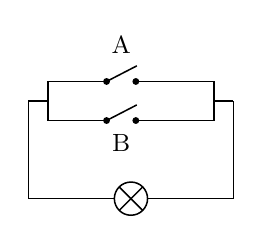
\begin{tikzpicture}[scale=0.62, line width=0.55pt]
  % 바깥 회로: 왼쪽 세로선 → 아래 가로선(전구) → 오른쪽 세로선
  \draw (0.4,2.2) -- (0.4,0.2) -- (2.16,0.2);
  \draw (2.84,0.2) -- (4.6,0.2) -- (4.6,2.2);
  % 바깥 회로와 병렬 블록을 잇는 선
  \draw (0.4,2.2) -- (0.8,2.2);
  \draw (0.8,1.8) -- (0.8,2.6);
  \draw (4.2,2.2) -- (4.6,2.2);
  \draw (4.2,1.8) -- (4.2,2.6);
  % 위 가지 · 스위치 A
  \draw (0.8,2.6) -- (2.0,2.6);
  \draw (2.6,2.6) -- (4.2,2.6);
  \draw (2.0,2.6) -- (2.62,2.92);
  \fill (2.0,2.6) circle (2pt);
  \fill (2.6,2.6) circle (2pt);
  \node[above, font=\small] at (2.3,2.96) {$\mathrm{A}$};
  % 아래 가지 · 스위치 B
  \draw (0.8,1.8) -- (2.0,1.8);
  \draw (2.6,1.8) -- (4.2,1.8);
  \draw (2.0,1.8) -- (2.62,2.12);
  \fill (2.0,1.8) circle (2pt);
  \fill (2.6,1.8) circle (2pt);
  \node[below, font=\small] at (2.3,1.72) {$\mathrm{B}$};
  % 전구
  \draw (2.5,0.2) circle (0.34);
  \draw (2.26,-0.04) -- (2.74,0.44);
  \draw (2.26,0.44) -- (2.74,-0.04);
\end{tikzpicture}
}\end{minipage}\par
\dmchoicesauto{}{$0.52$}{$0.56$}{$0.6$}{$0.64$}{$0.68$}
}\vspace{8mm}
\setcounter{dmproblemcount}{7}\dmpnum{80-08}{% id: 80-08
% book: 베이직쎈 확률과 통계 · 04 조건부확률
% section: 실전 감각 UP
% figure: none
% answer: 
% answer_source: 
% variant_level: 0 (원본 전사)
% 이 파일은 build.mjs 가 items.json 에서 만든다. 고칠 때는 items.json 을 고친다.
\smash{\raisebox{1.5mm}{\dmkichul{베이직쎈 확률과 통계 80쪽 08번}}}
$\mathrm{A}$, $\mathrm{B}$ 두 팀이 7번 경기를 하여 4번을 먼저 이기는 팀이 우승할 때, $\mathrm{A}$ 팀이 5번째 경기에서 우승할 확률은? \dmcondfill{두 팀이 이길 확률은 서로 같고, 비기는 경우는 생각하지 않는다.}{}
\begin{choicesii}{\rule[-3ex]{0pt}{8ex}$\dfrac{1}{16}$}{\rule[-3ex]{0pt}{8ex}$\dfrac{1}{8}$}{\rule[-3ex]{0pt}{8ex}$\dfrac{3}{16}$}{\rule[-3ex]{0pt}{8ex}$\dfrac{1}{4}$}{\rule[-3ex]{0pt}{8ex}$\dfrac{5}{16}$}\end{choicesii}
}\vspace{8mm}
\setcounter{dmproblemcount}{8}\dmpnum{80-09}{% id: 80-09
% book: 베이직쎈 확률과 통계 · 04 조건부확률
% section: 실전 감각 UP
% figure: none
% answer: 
% answer_source: 
% variant_level: 0 (원본 전사)
% 이 파일은 build.mjs 가 items.json 에서 만든다. 고칠 때는 items.json 을 고친다.
\smash{\raisebox{1.5mm}{\dmkichul{베이직쎈 확률과 통계 80쪽 09번 · 서답형}}}
어느 고등학교 $1$학년 학생 120명과 $2$학년 학생 200명은 음악 수업에서 북과 장구 중 반드시 하나를 선택하여 배운다고 한다. 장구를 선택한 $1$학년 학생은 76명이고, 북을 선택한 $2$학년 학생은 72명이다. 이 고등학교 $1$, $2$학년 학생 중 임의로 택한 한 명이 북을 선택한 학생일 때, 그 학생이 $1$학년일 확률을 구하시오.
}\vspace{8mm}
\vspace{3mm}\setcounter{dmproblemcount}{9}\dmpnum{80-10}{% id: 80-10
% book: 베이직쎈 확률과 통계 · 04 조건부확률
% section: 실전 감각 UP
% figure: none
% answer: 
% answer_source: 
% variant_level: 0 (원본 전사)
% 이 파일은 build.mjs 가 items.json 에서 만든다. 고칠 때는 items.json 을 고친다.
\smash{\raisebox{4.5mm}{\dmkichul{베이직쎈 확률과 통계 80쪽 10번 · 서술형}}}
파란 구슬 3개와 노란 구슬 $n$개가 들어 있는 주머니에서 임의로 구슬을 한 개씩 두 번 꺼낼 때, 첫 번째에 파란 구슬, 두 번째에 노란 구슬을 꺼낼 확률이 $\dfrac{1}{4}$이다. 이때 $n$의 값을 구하시오. \dmcondfill{$n>1$이고, 꺼낸 구슬은 다시 넣지 않는다.}{}
}\vspace{8mm}
\setcounter{dmproblemcount}{10}\dmpnum{80-11}{% id: 80-11
% book: 베이직쎈 확률과 통계 · 04 조건부확률
% section: 실전 감각 UP
% figure: none
% answer: 
% answer_source: 
% variant_level: 0 (원본 전사)
% 이 파일은 build.mjs 가 items.json 에서 만든다. 고칠 때는 items.json 을 고친다.
\smash{\raisebox{1.5mm}{\dmkichul{베이직쎈 확률과 통계 80쪽 11번}}}
흰 공 4개와 검은 공 2개가 들어 있는 $\mathrm{A}$ 주머니와 흰 공 3개와 검은 공 5개가 들어 있는 $\mathrm{B}$ 주머니가 있다. 한 개의 주사위를 던져서 나온 눈의 수가 $3$의 배수이면 $\mathrm{A}$ 주머니에서, $3$의 배수가 아니면 $\mathrm{B}$ 주머니에서 임의로 한 개의 공을 꺼내려고 한다. 꺼낸 공이 흰 공일 때, 이 공이 $\mathrm{A}$ 주머니에서 꺼낸 공일 확률을 구하시오.
}\vspace{8mm}
\setcounter{dmproblemcount}{11}\dmpnum{80-12}{% id: 80-12
% book: 베이직쎈 확률과 통계 · 04 조건부확률
% section: 실전 감각 UP
% figure: none
% answer: 
% answer_source: 
% variant_level: 0 (원본 전사)
% 이 파일은 build.mjs 가 items.json 에서 만든다. 고칠 때는 items.json 을 고친다.
\smash{\raisebox{1.5mm}{\dmkichul{베이직쎈 확률과 통계 80쪽 12번 · 서술형}}}
세 사건 $A$, $B$, $C$에 대하여 $A$와 $B$는 서로 독립이고, $A$와 $C$는 서로 배반사건이다. $\mathrm{P}(B)=0.7$, $\mathrm{P}(A\cap\comp{B})=0.15$, $\mathrm{P}(A\cup C)=0.6$일 때, $\mathrm{P}(C)$를 구하시오.
}\vspace{8mm}
\setcounter{dmproblemcount}{12}\dmpnum{80-13}{% id: 80-13
% book: 베이직쎈 확률과 통계 · 04 조건부확률
% section: 실전 감각 UP
% figure: tikz:fig-80-13
% answer: 
% answer_source: 
% variant_level: 0 (원본 전사)
% 이 파일은 build.mjs 가 items.json 에서 만든다. 고칠 때는 items.json 을 고친다.
\smash{\raisebox{1.5mm}{\dmkichul{베이직쎈 확률과 통계 80쪽 13번}}}
\noindent\begin{minipage}[t]{0.58\linewidth}\vspace{0pt}\raggedright 오른쪽 그림과 같이 한 변의 길이가 $1$인 정삼각형 $\mathrm{ABC}$의 변 위를 움직이는 점~$\mathrm{P}$가 있다. 한 개의 동전을 던져서 앞면이 나오면 점~$\mathrm{P}$를 시곗바늘이 도는 방향으로 $1$만큼, 뒷면이 나오면 시곗바늘이 도는 반대 방향으로 $1$만큼 움직인다고 할 때, 한 개의 동전을 3번 던져서 꼭짓점~$\mathrm{A}$에서 출발한 점~$\mathrm{P}$가 꼭짓점~$\mathrm{C}$에 있을 확률을 구하시오.\end{minipage}\hfill\begin{minipage}[t]{0.4\linewidth}\vspace{0pt}\centering \resizebox{\ifdim\width>\linewidth\linewidth\else\width\fi}{!}{% 80-13(인쇄 80쪽) — 한 변의 길이가 1인 정삼각형 ABC 와 변 위를 움직이는 점 P(출발점은 꼭짓점 A).
% C 에서 B 로 가는 점선 호와 그 옆의 1 은 「한 변만큼(=1) 움직인다」를 보인 원문 표시 그대로.
% 스캔 화질이 낮아 TikZ 로 다시 그림(점은 원문대로 A 자리 하나 · 라벨은 원문에 있는 A, B, C, P, 1 뿐 · 확률은 적지 않는다).
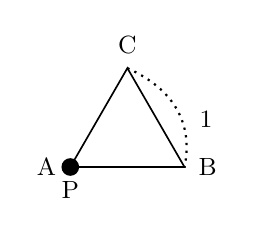
\begin{tikzpicture}[scale=1.45, line width=0.6pt]
  \coordinate (A) at (0,0);
  \coordinate (B) at (1,0);
  \coordinate (C) at (0.5,0.866);
  \draw (A) -- (B) -- (C) -- cycle;
  \fill (A) circle (2.2pt);
  \node[left=1.5pt, font=\small] at (A) {$\mathrm{A}$};
  \node[right=1.5pt, font=\small] at (B) {$\mathrm{B}$};
  \node[above=1.5pt, font=\small] at (C) {$\mathrm{C}$};
  \node[below=1.5pt, font=\small] at (A) {$\mathrm{P}$};
  \draw[dotted, line width=0.8pt] (C) .. controls (1.00,0.64) and (1.06,0.28) .. (B);
  \node[right=1pt, font=\small] at (1.02,0.42) {$1$};
\end{tikzpicture}
}\end{minipage}\par
}\vspace{8mm}
\setcounter{dmproblemcount}{13}\dmpnum{80-14}{% id: 80-14
% book: 베이직쎈 확률과 통계 · 04 조건부확률
% section: 실전 감각 UP
% figure: none
% answer: 
% answer_source: 
% variant_level: 0 (원본 전사)
% 이 파일은 build.mjs 가 items.json 에서 만든다. 고칠 때는 items.json 을 고친다.
\smash{\raisebox{1.5mm}{\dmkichul{베이직쎈 확률과 통계 80쪽 14번 · 서술형}}}
$1$부터 $8$까지의 자연수가 각각 하나씩 적힌 8개의 공이 들어 있는 주머니에서 임의로 한 개의 공을 꺼내어 숫자를 확인하고 다시 넣는 시행을 5번 반복할 때, $4$의 배수가 적힌 공을 4번 미만 꺼낼 확률을 구하시오.
}\vspace{8mm}
\vspace*{0pt plus 1filll}
\clearpage
\renewcommand{\dmchapunit}{05 확률변수와 확률분포}
\dmchapter{05}{확률변수와 확률분포}
\setcounter{dmproblemcount}{0}
\dmsection{개념 23 확률변수와 확률분포}
\dmpassage{다음 확률변수 $X$가 가질 수 있는 값을 모두 구하시오.}
\setcounter{dmproblemcount}{0}\dmpnum{82-01}{% id: 82-01
% book: 베이직쎈 확률과 통계 · 05 확률변수와 확률분포
% section: 개념 23 확률변수와 확률분포
% passage: 다음 확률변수 $X$가 가질 수 있는 값을 모두 구하시오.
% figure: none
% answer: 
% answer_source: 
% variant_level: 0 (원본 전사)
% 이 파일은 build.mjs 가 items.json 에서 만든다. 고칠 때는 items.json 을 고친다.
\smash{\raisebox{1.5mm}{\dmkichul{베이직쎈 확률과 통계 82쪽 01번}}}
서로 다른 3개의 동전을 동시에 던질 때, 뒷면이 나오는 동전의 개수 $X$
\dmhint{동전의 앞면을 $\mathrm{H}$, 뒷면을 $\mathrm{T}$라 할 때, 표본공간 $S$는\\[3pt] $S=\{\mathrm{HHH}{,}\mkern3mu\mathopen{}\mathrm{HHT}{,}\mkern3mu\mathopen{}\blank[2.4em]{,}\mkern3mu\mathopen{}\mathrm{HTT}{,}\mkern3mu\mathopen{}\mathrm{THH}{,}\mkern3mu\mathopen{}\blank[2.4em],$\\[3pt] $\blank[2.4em]{,}\mkern3mu\mathopen{}\blank[2.4em]\}$\\[3pt] 따라서 $X$가 가질 수 있는 값은 \quad $0$, $\blank$, $\blank$, $\blank$}
}\vspace{8mm}
\setcounter{dmproblemcount}{1}\dmpnum{82-02}{% id: 82-02
% book: 베이직쎈 확률과 통계 · 05 확률변수와 확률분포
% section: 개념 23 확률변수와 확률분포
% passage: 다음 확률변수 $X$가 가질 수 있는 값을 모두 구하시오.
% figure: none
% answer: 
% answer_source: 
% variant_level: 0 (원본 전사)
% 이 파일은 build.mjs 가 items.json 에서 만든다. 고칠 때는 items.json 을 고친다.
\smash{\raisebox{1.5mm}{\dmkichul{베이직쎈 확률과 통계 82쪽 02번}}}
한 개의 주사위를 던질 때, 나오는 눈의 수 $X$
}\vspace{8mm}
\setcounter{dmproblemcount}{2}\dmpnum{82-03}{% id: 82-03
% book: 베이직쎈 확률과 통계 · 05 확률변수와 확률분포
% section: 개념 23 확률변수와 확률분포
% passage: 다음 확률변수 $X$가 가질 수 있는 값을 모두 구하시오.
% figure: none
% answer: 
% answer_source: 
% variant_level: 0 (원본 전사)
% 이 파일은 build.mjs 가 items.json 에서 만든다. 고칠 때는 items.json 을 고친다.
\smash{\raisebox{1.5mm}{\dmkichul{베이직쎈 확률과 통계 82쪽 03번}}}
한 개의 주사위를 4번 던질 때, 3의 눈이 나오는 횟수 $X$
}\vspace{8mm}
\setcounter{dmproblemcount}{3}\dmpnum{82-04}{% id: 82-04
% book: 베이직쎈 확률과 통계 · 05 확률변수와 확률분포
% section: 개념 23 확률변수와 확률분포
% passage: 다음 확률변수 $X$가 가질 수 있는 값을 모두 구하시오.
% figure: none
% answer: 
% answer_source: 
% variant_level: 0 (원본 전사)
% 이 파일은 build.mjs 가 items.json 에서 만든다. 고칠 때는 items.json 을 고친다.
\smash{\raisebox{1.5mm}{\dmkichul{베이직쎈 확률과 통계 82쪽 04번}}}
페널티 킥을 5번 시도할 때, 성공한 횟수 $X$
}\vspace{8mm}
\dmpassage{다음 확률변수 $X$의 확률분포를 표로 나타내시오.}
\setcounter{dmproblemcount}{4}\dmpnum{82-05}{% id: 82-05
% book: 베이직쎈 확률과 통계 · 05 확률변수와 확률분포
% section: 개념 23 확률변수와 확률분포
% passage: 다음 확률변수 $X$의 확률분포를 표로 나타내시오.
% figure: none
% answer: 
% answer_source: 
% variant_level: 0 (원본 전사)
% 이 파일은 build.mjs 가 items.json 에서 만든다. 고칠 때는 items.json 을 고친다.
\smash{\raisebox{1.5mm}{\dmkichul{베이직쎈 확률과 통계 82쪽 05번}}}
한 개의 주사위를 두 번 던질 때, 4의 눈이 나오는 횟수 $X$\par\smallskip\dispeq{{\setlength{\tabcolsep}{7pt}\renewcommand{\arraystretch}{1.9}\begin{tabular}{|c|c|c|c|c|}\hline $X$ & \makebox[2.6em]{} & \makebox[2.6em]{} & \makebox[2.6em]{} & 합계 \\ \hline $\mathrm{P}(X=x)$ & & & & \\ \hline\end{tabular}}}
}\vspace{8mm}
\setcounter{dmproblemcount}{5}\dmpnum{82-06}{% id: 82-06
% book: 베이직쎈 확률과 통계 · 05 확률변수와 확률분포
% section: 개념 23 확률변수와 확률분포
% passage: 다음 확률변수 $X$의 확률분포를 표로 나타내시오.
% figure: none
% answer: 
% answer_source: 
% variant_level: 0 (원본 전사)
% 이 파일은 build.mjs 가 items.json 에서 만든다. 고칠 때는 items.json 을 고친다.
\smash{\raisebox{1.5mm}{\dmkichul{베이직쎈 확률과 통계 82쪽 06번}}}
한 개의 주사위를 두 번 던질 때, 홀수의 눈이 나오는 횟수 $X$
}\vspace{8mm}
\setcounter{dmproblemcount}{6}\dmpnum{82-07}{% id: 82-07
% book: 베이직쎈 확률과 통계 · 05 확률변수와 확률분포
% section: 개념 23 확률변수와 확률분포
% passage: 다음 확률변수 $X$의 확률분포를 표로 나타내시오.
% figure: none
% answer: 
% answer_source: 
% variant_level: 0 (원본 전사)
% 이 파일은 build.mjs 가 items.json 에서 만든다. 고칠 때는 items.json 을 고친다.
\smash{\raisebox{1.5mm}{\dmkichul{베이직쎈 확률과 통계 82쪽 07번}}}
2개의 당첨 제비를 포함한 6개의 제비 중에서 임의로 2개의 제비를 동시에 뽑을 때, 뽑힌 당첨 제비의 개수 $X$
}\vspace{8mm}
\dmsection{개념 24 이산확률변수와 확률질량함수}
\vspace{5mm}\setcounter{dmproblemcount}{7}\dmpnum{83-08}{% id: 83-08
% book: 베이직쎈 확률과 통계 · 05 확률변수와 확률분포
% section: 개념 24 이산확률변수와 확률질량함수
% figure: none
% answer: 
% answer_source: 
% variant_level: 0 (원본 전사)
% 이 파일은 build.mjs 가 items.json 에서 만든다. 고칠 때는 items.json 을 고친다.
\smash{\raisebox{6.5mm}{\dmkichul{베이직쎈 확률과 통계 83쪽 08번}}}
확률변수 $X$의 확률질량함수가\par\smallskip\dispeq{$\mathrm{P}(X=x)=\begin{cases} \dfrac{3}{10} & (x=1{,}\mkern3mu\mathopen{}3) \\[9pt] \dfrac{2}{5} & (x=2) \end{cases}$}\par\smallskip\noindent 일 때, 다음 표를 완성하시오.\par\smallskip\dispeq{{\setlength{\tabcolsep}{7pt}\renewcommand{\arraystretch}{1.9}\begin{tabular}{|c|c|c|c|c|}\hline $X$ & \makebox[2.6em]{} & \makebox[2.6em]{} & \makebox[2.6em]{} & 합계 \\ \hline $\mathrm{P}(X=x)$ & & & & \\ \hline\end{tabular}}}
}\vspace{8mm}
\setcounter{dmproblemcount}{8}\dmpnum{83-09}{% id: 83-09
% book: 베이직쎈 확률과 통계 · 05 확률변수와 확률분포
% section: 개념 24 이산확률변수와 확률질량함수
% figure: none
% answer: 
% answer_source: 
% variant_level: 0 (원본 전사)
% 이 파일은 build.mjs 가 items.json 에서 만든다. 고칠 때는 items.json 을 고친다.
\smash{\raisebox{1.5mm}{\dmkichul{베이직쎈 확률과 통계 83쪽 09번}}}
한 개의 동전을 세 번 던지는 시행에서 뒷면이 나오는 횟수를 확률변수 $X$라 하자. 다음을 구하시오.
\dmsubprob{1} $X$의 확률질량함수\\[3pt] $\mathrm{P}(X=x)={}_{\text{\scriptsize\setlength{\fboxsep}{1.5pt}\framebox[1.5em]{\rule{0pt}{1.6ex}}}}\mathrm{C}_x\left(\blank\right)^{x}\left(\dfrac{1}{2}\right)^{\text{\scriptsize\setlength{\fboxsep}{1.5pt}\framebox[1.5em]{\rule{0pt}{1.6ex}}}}{}^{-x}$\\[5pt] $\hphantom{\mathrm{P}(X=x)}={}_{\text{\scriptsize\setlength{\fboxsep}{1.5pt}\framebox[1.5em]{\rule{0pt}{1.6ex}}}}\mathrm{C}_x\left(\blank\right)^{3}$ $(x=0{,}\mkern3mu\mathopen{}\blank{,}\mkern3mu\mathopen{}2{,}\mkern3mu\mathopen{}\blank)$
\dmsubprob{2} $X$의 확률분포를 나타낸 표\par\smallskip\centerline{{\setlength{\tabcolsep}{7pt}\renewcommand{\arraystretch}{1.9}\begin{tabular}{|c|c|c|c|c|c|}\hline $X$ & \makebox[2.6em]{} & \makebox[2.6em]{} & \makebox[2.6em]{} & \makebox[2.6em]{} & 합계 \\ \hline $\mathrm{P}(X=x)$ & & & & & \\ \hline\end{tabular}}}
}\vspace{8mm}
\setcounter{dmproblemcount}{9}\dmpnum{83-10}{% id: 83-10
% book: 베이직쎈 확률과 통계 · 05 확률변수와 확률분포
% section: 개념 24 이산확률변수와 확률질량함수
% figure: none
% answer: 
% answer_source: 
% variant_level: 0 (원본 전사)
% 이 파일은 build.mjs 가 items.json 에서 만든다. 고칠 때는 items.json 을 고친다.
\smash{\raisebox{1.5mm}{\dmkichul{베이직쎈 확률과 통계 83쪽 10번}}}
한 개의 주사위를 두 번 던질 때, 5의 약수의 눈이 나오는 횟수를 확률변수 $X$라 하자. 다음을 구하시오.
\dmsubprob{1} $X$의 확률질량함수
\dmsubprob{2} $X$의 확률분포를 나타낸 표
}\vspace{8mm}
\setcounter{dmproblemcount}{10}\dmpnum{83-11}{% id: 83-11
% book: 베이직쎈 확률과 통계 · 05 확률변수와 확률분포
% section: 개념 24 이산확률변수와 확률질량함수
% figure: none
% answer: 
% answer_source: 
% variant_level: 0 (원본 전사)
% 이 파일은 build.mjs 가 items.json 에서 만든다. 고칠 때는 items.json 을 고친다.
\smash{\raisebox{1.5mm}{\dmkichul{베이직쎈 확률과 통계 83쪽 11번}}}
빨간 공 2개, 파란 공 3개가 들어 있는 주머니에서 임의로 2개의 공을 동시에 꺼낼 때, 꺼낸 빨간 공의 개수를 확률변수 $X$라 하자. 다음을 구하시오.
\dmsubprob{1} $X$의 확률질량함수
\dmsubprob{2} $X$의 확률분포를 나타낸 표
}\vspace{8mm}
\dmpassage{확률변수 $X$의 확률질량함수가\par\smallskip\centerline{$\mathrm{P}(X=x)=\begin{cases} \dfrac{1}{8} & (x=1) \\[9pt] \dfrac{1}{4} & (x=2{,}\mkern3mu\mathopen{}4) \\[9pt] \dfrac{3}{8} & (x=3) \end{cases}$}\par\smallskip\noindent 일 때, 다음을 구하시오.}
\setcounter{dmproblemcount}{11}\dmpnum{84-12}{% id: 84-12
% book: 베이직쎈 확률과 통계 · 05 확률변수와 확률분포
% section: 개념 24 이산확률변수와 확률질량함수
% passage: 확률변수 $X$의 확률질량함수가\par\smallskip\centerline{$\mathrm{P}(X=x)=\begin{cases} \dfrac{1}{8} & (x=1) \\[9pt] \dfrac{1}{4} & (x=2{,}\mkern3mu\mathopen{}4) \\[9pt] \dfrac{3}{8} & (x=3) \end{cases}$}\par\smallskip\noindent 일 때, 다음을 구하시오.
% figure: none
% answer: 
% answer_source: 
% variant_level: 0 (원본 전사)
% 이 파일은 build.mjs 가 items.json 에서 만든다. 고칠 때는 items.json 을 고친다.
\smash{\raisebox{1.5mm}{\dmkichul{베이직쎈 확률과 통계 84쪽 12번}}}
$\mathrm{P}(X=4)$
}\vspace{8mm}
\setcounter{dmproblemcount}{12}\dmpnum{84-13}{% id: 84-13
% book: 베이직쎈 확률과 통계 · 05 확률변수와 확률분포
% section: 개념 24 이산확률변수와 확률질량함수
% passage: 확률변수 $X$의 확률질량함수가\par\smallskip\centerline{$\mathrm{P}(X=x)=\begin{cases} \dfrac{1}{8} & (x=1) \\[9pt] \dfrac{1}{4} & (x=2{,}\mkern3mu\mathopen{}4) \\[9pt] \dfrac{3}{8} & (x=3) \end{cases}$}\par\smallskip\noindent 일 때, 다음을 구하시오.
% figure: none
% answer: 
% answer_source: 
% variant_level: 0 (원본 전사)
% 이 파일은 build.mjs 가 items.json 에서 만든다. 고칠 때는 items.json 을 고친다.
\smash{\raisebox{1.5mm}{\dmkichul{베이직쎈 확률과 통계 84쪽 13번}}}
$\mathrm{P}(X=2)+\mathrm{P}(X=3)$
}\vspace{8mm}
\setcounter{dmproblemcount}{13}\dmpnum{84-14}{% id: 84-14
% book: 베이직쎈 확률과 통계 · 05 확률변수와 확률분포
% section: 개념 24 이산확률변수와 확률질량함수
% passage: 확률변수 $X$의 확률질량함수가\par\smallskip\centerline{$\mathrm{P}(X=x)=\begin{cases} \dfrac{1}{8} & (x=1) \\[9pt] \dfrac{1}{4} & (x=2{,}\mkern3mu\mathopen{}4) \\[9pt] \dfrac{3}{8} & (x=3) \end{cases}$}\par\smallskip\noindent 일 때, 다음을 구하시오.
% figure: none
% answer: 
% answer_source: 
% variant_level: 0 (원본 전사)
% 이 파일은 build.mjs 가 items.json 에서 만든다. 고칠 때는 items.json 을 고친다.
\smash{\raisebox{1.5mm}{\dmkichul{베이직쎈 확률과 통계 84쪽 14번}}}
$\mathrm{P}(1\le X\le 3)$
}\vspace{8mm}
\setcounter{dmproblemcount}{14}\dmpnum{84-15}{% id: 84-15
% book: 베이직쎈 확률과 통계 · 05 확률변수와 확률분포
% section: 개념 24 이산확률변수와 확률질량함수
% passage: 확률변수 $X$의 확률질량함수가\par\smallskip\centerline{$\mathrm{P}(X=x)=\begin{cases} \dfrac{1}{8} & (x=1) \\[9pt] \dfrac{1}{4} & (x=2{,}\mkern3mu\mathopen{}4) \\[9pt] \dfrac{3}{8} & (x=3) \end{cases}$}\par\smallskip\noindent 일 때, 다음을 구하시오.
% figure: none
% answer: 
% answer_source: 
% variant_level: 0 (원본 전사)
% 이 파일은 build.mjs 가 items.json 에서 만든다. 고칠 때는 items.json 을 고친다.
\smash{\raisebox{1.5mm}{\dmkichul{베이직쎈 확률과 통계 84쪽 15번}}}
$\mathrm{P}(X\ge 2)$
}\vspace{8mm}
\dmpassage{확률변수 $X$의 확률분포를 표로 나타내면 아래와 같을 때, 다음을 구하시오.}
\begin{center}\resizebox{\ifdim\width>\linewidth\linewidth\else\width\fi}{!}{% 개념 24 84-16~19(인쇄 84쪽) — 공통 지시문의 확률분포표. 스캔 표라 tabular 로 다시 조판(칸 값 원문 그대로).
{\setlength{\tabcolsep}{7pt}\renewcommand{\arraystretch}{2.2}%
\begin{tabular}{|c|c|c|c|c|c|c|}
\hline
$X$ & $-1$ & $0$ & $1$ & $2$ & $3$ & 합계 \\
\hline
$\mathrm{P}(X=x)$ & $\dfrac{1}{12}$ & $\dfrac{1}{6}$ & $\dfrac{1}{3}$ & $\dfrac{1}{6}$ & $\dfrac{1}{4}$ & $1$ \\
\hline
\end{tabular}}
}\end{center}\vspace{4mm}
\setcounter{dmproblemcount}{15}\dmpnum{84-16}{% id: 84-16
% book: 베이직쎈 확률과 통계 · 05 확률변수와 확률분포
% section: 개념 24 이산확률변수와 확률질량함수
% passage: 확률변수 $X$의 확률분포를 표로 나타내면 아래와 같을 때, 다음을 구하시오.
% figure: tikz:fig-84-16
% answer: 
% answer_source: 
% variant_level: 0 (원본 전사)
% 이 파일은 build.mjs 가 items.json 에서 만든다. 고칠 때는 items.json 을 고친다.
\smash{\raisebox{1.5mm}{\dmkichul{베이직쎈 확률과 통계 84쪽 16번}}}
$\mathrm{P}(X=1$ 또는 $X=3)$
}\vspace{8mm}
\setcounter{dmproblemcount}{16}\dmpnum{84-17}{% id: 84-17
% book: 베이직쎈 확률과 통계 · 05 확률변수와 확률분포
% section: 개념 24 이산확률변수와 확률질량함수
% passage: 확률변수 $X$의 확률분포를 표로 나타내면 아래와 같을 때, 다음을 구하시오.
% figure: tikz:fig-84-16
% answer: 
% answer_source: 
% variant_level: 0 (원본 전사)
% 이 파일은 build.mjs 가 items.json 에서 만든다. 고칠 때는 items.json 을 고친다.
\smash{\raisebox{1.5mm}{\dmkichul{베이직쎈 확률과 통계 84쪽 17번}}}
$\mathrm{P}(1\le X\le 2)$
}\vspace{8mm}
\setcounter{dmproblemcount}{17}\dmpnum{84-18}{% id: 84-18
% book: 베이직쎈 확률과 통계 · 05 확률변수와 확률분포
% section: 개념 24 이산확률변수와 확률질량함수
% passage: 확률변수 $X$의 확률분포를 표로 나타내면 아래와 같을 때, 다음을 구하시오.
% figure: tikz:fig-84-16
% answer: 
% answer_source: 
% variant_level: 0 (원본 전사)
% 이 파일은 build.mjs 가 items.json 에서 만든다. 고칠 때는 items.json 을 고친다.
\smash{\raisebox{1.5mm}{\dmkichul{베이직쎈 확률과 통계 84쪽 18번}}}
$\mathrm{P}(X\le 1)$
}\vspace{8mm}
\setcounter{dmproblemcount}{18}\dmpnum{84-19}{% id: 84-19
% book: 베이직쎈 확률과 통계 · 05 확률변수와 확률분포
% section: 개념 24 이산확률변수와 확률질량함수
% passage: 확률변수 $X$의 확률분포를 표로 나타내면 아래와 같을 때, 다음을 구하시오.
% figure: tikz:fig-84-16
% answer: 
% answer_source: 
% variant_level: 0 (원본 전사)
% 이 파일은 build.mjs 가 items.json 에서 만든다. 고칠 때는 items.json 을 고친다.
\smash{\raisebox{1.5mm}{\dmkichul{베이직쎈 확률과 통계 84쪽 19번}}}
$\mathrm{P}(X^2-2X=0)$
}\vspace{8mm}
\dmpassage{확률변수 $X$의 확률분포를 표로 나타내면 다음과 같을 때, 상수 $a$의 값을 구하시오.}
\setcounter{dmproblemcount}{19}\dmpnum{84-20}{% id: 84-20
% book: 베이직쎈 확률과 통계 · 05 확률변수와 확률분포
% section: 개념 24 이산확률변수와 확률질량함수
% passage: 확률변수 $X$의 확률분포를 표로 나타내면 다음과 같을 때, 상수 $a$의 값을 구하시오.
% figure: none
% answer: 
% answer_source: 
% variant_level: 0 (원본 전사)
% 이 파일은 build.mjs 가 items.json 에서 만든다. 고칠 때는 items.json 을 고친다.
\smash{\raisebox{1.5mm}{\dmkichul{베이직쎈 확률과 통계 84쪽 20번}}}
\par\smallskip\dispeq{{\setlength{\tabcolsep}{7pt}\renewcommand{\arraystretch}{2.2}\begin{tabular}{|c|c|c|c|c|}\hline $X$ & $2$ & $4$ & $6$ & 합계 \\ \hline $\mathrm{P}(X=x)$ & $a$ & $\dfrac{3}{7}$ & $\dfrac{2}{7}$ & $1$ \\ \hline\end{tabular}}}
}\vspace{8mm}
\setcounter{dmproblemcount}{20}\dmpnum{84-21}{% id: 84-21
% book: 베이직쎈 확률과 통계 · 05 확률변수와 확률분포
% section: 개념 24 이산확률변수와 확률질량함수
% passage: 확률변수 $X$의 확률분포를 표로 나타내면 다음과 같을 때, 상수 $a$의 값을 구하시오.
% figure: none
% answer: 
% answer_source: 
% variant_level: 0 (원본 전사)
% 이 파일은 build.mjs 가 items.json 에서 만든다. 고칠 때는 items.json 을 고친다.
\smash{\raisebox{1.5mm}{\dmkichul{베이직쎈 확률과 통계 84쪽 21번}}}
\par\smallskip\dispeq{{\setlength{\tabcolsep}{7pt}\renewcommand{\arraystretch}{2.2}\begin{tabular}{|c|c|c|c|c|c|}\hline $X$ & $-3$ & $-1$ & $1$ & $3$ & 합계 \\ \hline $\mathrm{P}(X=x)$ & $\dfrac{2}{9}$ & $a$ & $\dfrac{1}{3}$ & $\dfrac{1}{9}$ & $1$ \\ \hline\end{tabular}}}
}\vspace{8mm}
\setcounter{dmproblemcount}{21}\dmpnum{84-22}{% id: 84-22
% book: 베이직쎈 확률과 통계 · 05 확률변수와 확률분포
% section: 개념 24 이산확률변수와 확률질량함수
% passage: 확률변수 $X$의 확률분포를 표로 나타내면 다음과 같을 때, 상수 $a$의 값을 구하시오.
% figure: none
% answer: 
% answer_source: 
% variant_level: 0 (원본 전사)
% 이 파일은 build.mjs 가 items.json 에서 만든다. 고칠 때는 items.json 을 고친다.
\smash{\raisebox{1.5mm}{\dmkichul{베이직쎈 확률과 통계 84쪽 22번}}}
\par\smallskip\dispeq{{\setlength{\tabcolsep}{7pt}\renewcommand{\arraystretch}{2.2}\begin{tabular}{|c|c|c|c|c|c|c|}\hline $X$ & $0$ & $1$ & $3$ & $5$ & $7$ & 합계 \\ \hline $\mathrm{P}(X=x)$ & $\dfrac{1}{3}$ & $\dfrac{1}{15}$ & $3a$ & $\dfrac{2}{15}$ & $\dfrac{4}{15}$ & $1$ \\ \hline\end{tabular}}}
}\vspace{8mm}
\dmpassage{확률변수 $X$의 확률질량함수가 다음과 같을 때, 상수 $k$의 값을 구하시오.}
\setcounter{dmproblemcount}{22}\dmpnum{84-23}{% id: 84-23
% book: 베이직쎈 확률과 통계 · 05 확률변수와 확률분포
% section: 개념 24 이산확률변수와 확률질량함수
% passage: 확률변수 $X$의 확률질량함수가 다음과 같을 때, 상수 $k$의 값을 구하시오.
% figure: none
% answer: 
% answer_source: 
% variant_level: 0 (원본 전사)
% 이 파일은 build.mjs 가 items.json 에서 만든다. 고칠 때는 items.json 을 고친다.
\smash{\raisebox{1.5mm}{\dmkichul{베이직쎈 확률과 통계 84쪽 23번}}}
$\mathrm{P}(X=x)=kx$ $(x=1{,}\mkern3mu\mathopen{}2{,}\mkern3mu\mathopen{}3)$
\dmhint{확률의 총합은 $\blank$이므로\\[3pt] $\mathrm{P}(X=1)+\mathrm{P}(X=\blank)+\mathrm{P}(X=3)=\blank$\\[3pt] $k+2k+\blank=\blank$, \quad $\blank=1$\\[3pt] $\therefore\ k=\blank$}
}\vspace{8mm}
\setcounter{dmproblemcount}{23}\dmpnum{84-24}{% id: 84-24
% book: 베이직쎈 확률과 통계 · 05 확률변수와 확률분포
% section: 개념 24 이산확률변수와 확률질량함수
% passage: 확률변수 $X$의 확률질량함수가 다음과 같을 때, 상수 $k$의 값을 구하시오.
% figure: none
% answer: 
% answer_source: 
% variant_level: 0 (원본 전사)
% 이 파일은 build.mjs 가 items.json 에서 만든다. 고칠 때는 items.json 을 고친다.
\smash{\raisebox{1.5mm}{\dmkichul{베이직쎈 확률과 통계 84쪽 24번}}}
$\mathrm{P}(X=x)=k(x+2)$ $(x=-1{,}\mkern3mu\mathopen{}0{,}\mkern3mu\mathopen{}1{,}\mkern3mu\mathopen{}2)$
}\vspace{8mm}
\setcounter{dmproblemcount}{24}\dmpnum{84-25}{% id: 84-25
% book: 베이직쎈 확률과 통계 · 05 확률변수와 확률분포
% section: 개념 24 이산확률변수와 확률질량함수
% passage: 확률변수 $X$의 확률질량함수가 다음과 같을 때, 상수 $k$의 값을 구하시오.
% figure: none
% answer: 
% answer_source: 
% variant_level: 0 (원본 전사)
% 이 파일은 build.mjs 가 items.json 에서 만든다. 고칠 때는 items.json 을 고친다.
\smash{\raisebox{1.5mm}{\dmkichul{베이직쎈 확률과 통계 84쪽 25번}}}
$\mathrm{P}(X=x)=kx^2$ $(x=1{,}\mkern3mu\mathopen{}2{,}\mkern3mu\mathopen{}3{,}\mkern3mu\mathopen{}4)$
}\vspace{8mm}
\vspace{3mm}\setcounter{dmproblemcount}{25}\dmpnum{84-26}{% id: 84-26
% book: 베이직쎈 확률과 통계 · 05 확률변수와 확률분포
% section: 개념 24 이산확률변수와 확률질량함수
% passage: 확률변수 $X$의 확률질량함수가 다음과 같을 때, 상수 $k$의 값을 구하시오.
% figure: none
% answer: 
% answer_source: 
% variant_level: 0 (원본 전사)
% 이 파일은 build.mjs 가 items.json 에서 만든다. 고칠 때는 items.json 을 고친다.
\smash{\raisebox{4.5mm}{\dmkichul{베이직쎈 확률과 통계 84쪽 26번}}}
$\mathrm{P}(X=x)=\dfrac{k}{x}$ $(x=1{,}\mkern3mu\mathopen{}2{,}\mkern3mu\mathopen{}4)$
}\vspace{8mm}
\dmsection{개념 25 연속확률변수와 확률밀도함수}
\dmpassage{다음 확률변수 $X$가 연속확률변수이면 ‘연’을, 이산확률변수이면 ‘이’를 ( ) 안에 써넣으시오.}
\setcounter{dmproblemcount}{26}\dmpnum{85-27}{% id: 85-27
% book: 베이직쎈 확률과 통계 · 05 확률변수와 확률분포
% section: 개념 25 연속확률변수와 확률밀도함수
% passage: 다음 확률변수 $X$가 연속확률변수이면 ‘연’을, 이산확률변수이면 ‘이’를 ( ) 안에 써넣으시오.
% figure: none
% answer: 
% answer_source: 
% variant_level: 0 (원본 전사)
% 이 파일은 build.mjs 가 items.json 에서 만든다. 고칠 때는 items.json 을 고친다.
\smash{\raisebox{1.5mm}{\dmkichul{베이직쎈 확률과 통계 85쪽 27번}}}
서로 다른 동전 두 개를 동시에 던질 때, 앞면이 나오는 동전의 개수 $X$ \hfill (\hspace*{2.4em})
}\vspace{8mm}
\setcounter{dmproblemcount}{27}\dmpnum{85-28}{% id: 85-28
% book: 베이직쎈 확률과 통계 · 05 확률변수와 확률분포
% section: 개념 25 연속확률변수와 확률밀도함수
% passage: 다음 확률변수 $X$가 연속확률변수이면 ‘연’을, 이산확률변수이면 ‘이’를 ( ) 안에 써넣으시오.
% figure: none
% answer: 
% answer_source: 
% variant_level: 0 (원본 전사)
% 이 파일은 build.mjs 가 items.json 에서 만든다. 고칠 때는 items.json 을 고친다.
\smash{\raisebox{1.5mm}{\dmkichul{베이직쎈 확률과 통계 85쪽 28번}}}
어느 고등학교 2학년 학생들의 키 $X$ \hfill (\hspace*{2.4em})
}\vspace{8mm}
\setcounter{dmproblemcount}{28}\dmpnum{85-29}{% id: 85-29
% book: 베이직쎈 확률과 통계 · 05 확률변수와 확률분포
% section: 개념 25 연속확률변수와 확률밀도함수
% passage: 다음 확률변수 $X$가 연속확률변수이면 ‘연’을, 이산확률변수이면 ‘이’를 ( ) 안에 써넣으시오.
% figure: none
% answer: 
% answer_source: 
% variant_level: 0 (원본 전사)
% 이 파일은 build.mjs 가 items.json 에서 만든다. 고칠 때는 items.json 을 고친다.
\smash{\raisebox{1.5mm}{\dmkichul{베이직쎈 확률과 통계 85쪽 29번}}}
가위바위보를 5번 하는 시행에서 비긴 횟수 $X$ \hfill (\hspace*{2.4em})
}\vspace{8mm}
\setcounter{dmproblemcount}{29}\dmpnum{85-30}{% id: 85-30
% book: 베이직쎈 확률과 통계 · 05 확률변수와 확률분포
% section: 개념 25 연속확률변수와 확률밀도함수
% passage: 다음 확률변수 $X$가 연속확률변수이면 ‘연’을, 이산확률변수이면 ‘이’를 ( ) 안에 써넣으시오.
% figure: none
% answer: 
% answer_source: 
% variant_level: 0 (원본 전사)
% 이 파일은 build.mjs 가 items.json 에서 만든다. 고칠 때는 items.json 을 고친다.
\smash{\raisebox{1.5mm}{\dmkichul{베이직쎈 확률과 통계 85쪽 30번}}}
남학생 5명과 여학생 3명 중에서 임의로 2명의 대표를 뽑을 때, 뽑힌 여학생 수 $X$ \hfill (\hspace*{2.4em})
}\vspace{8mm}
\setcounter{dmproblemcount}{30}\dmpnum{85-31}{% id: 85-31
% book: 베이직쎈 확률과 통계 · 05 확률변수와 확률분포
% section: 개념 25 연속확률변수와 확률밀도함수
% passage: 다음 확률변수 $X$가 연속확률변수이면 ‘연’을, 이산확률변수이면 ‘이’를 ( ) 안에 써넣으시오.
% figure: none
% answer: 
% answer_source: 
% variant_level: 0 (원본 전사)
% 이 파일은 build.mjs 가 items.json 에서 만든다. 고칠 때는 items.json 을 고친다.
\smash{\raisebox{1.5mm}{\dmkichul{베이직쎈 확률과 통계 85쪽 31번}}}
어느 정거장에서 10분 간격으로 도착하는 버스를 기다리는 시간 $X$ \hfill (\hspace*{2.4em})
}\vspace{8mm}
\setcounter{dmproblemcount}{31}\dmpnum{85-32}{% id: 85-32
% book: 베이직쎈 확률과 통계 · 05 확률변수와 확률분포
% section: 개념 25 연속확률변수와 확률밀도함수
% passage: 다음 확률변수 $X$가 연속확률변수이면 ‘연’을, 이산확률변수이면 ‘이’를 ( ) 안에 써넣으시오.
% figure: none
% answer: 
% answer_source: 
% variant_level: 0 (원본 전사)
% 이 파일은 build.mjs 가 items.json 에서 만든다. 고칠 때는 items.json 을 고친다.
\smash{\raisebox{1.5mm}{\dmkichul{베이직쎈 확률과 통계 85쪽 32번}}}
어느 지역에서 한 달 동안 내린 강우량 $X$ \hfill (\hspace*{2.4em})
}\vspace{8mm}
\dmpassage{다음 중 $f(x)$가 $0\le X\le 2$에서 모든 실수의 값을 갖는 연속확률변수 $X$의 확률밀도함수가 될 수 있는 것은 ‘○’를, 될 수 없는 것은 ‘×’를 ( ) 안에 써넣으시오.}
\setcounter{dmproblemcount}{32}\dmpnum{85-33}{% id: 85-33
% book: 베이직쎈 확률과 통계 · 05 확률변수와 확률분포
% section: 개념 25 연속확률변수와 확률밀도함수
% passage: 다음 중 $f(x)$가 $0\le X\le 2$에서 모든 실수의 값을 갖는 연속확률변수 $X$의 확률밀도함수가 될 수 있는 것은 ‘○’를, 될 수 없는 것은 ‘×’를 ( ) 안에 써넣으시오.
% figure: tikz:fig-85-33
% answer: 
% answer_source: 
% variant_level: 0 (원본 전사)
% 이 파일은 build.mjs 가 items.json 에서 만든다. 고칠 때는 items.json 을 고친다.
\smash{\raisebox{1.5mm}{\dmkichul{베이직쎈 확률과 통계 85쪽 33번}}}
\noindent\begin{minipage}[t]{0.58\linewidth}\vspace{0pt}\raggedright \hspace*{\stretch{10}}(\hspace*{2.4em})\end{minipage}\hfill\begin{minipage}[t]{0.4\linewidth}\vspace{0pt}\centering \resizebox{\ifdim\width>\linewidth\linewidth\else\width\fi}{!}{% 개념 25 85-33(인쇄 85쪽) — 확률밀도함수가 될 수 있는지 묻는 그래프: 0≤x≤2 에서 y=2 인 가로 선분과 x=2 의 점선.
% 스캔 화질이 낮아 TikZ 로 다시 그림. 축 0.7pt · 그래프 0.6pt · 라벨은 원문에 있는 것만(O · x · y · 2 · y=f(x)).
\begin{tikzpicture}[scale=0.75, line width=0.6pt]
  \draw[->, line width=0.7pt] (-0.45,0) -- (2.95,0) node[below, font=\small] {$x$};
  \draw[->, line width=0.7pt] (0,-0.5) -- (0,2.75) node[right, font=\small] {$y$};
  \node[below left=-2pt and -2pt, font=\small] at (0,0) {$\mathrm{O}$};
  \draw[dotted, line width=0.6pt] (2,0) -- (2,2);
  \draw (0,2) -- (2,2);
  \node[left, font=\small] at (0,2) {$2$};
  \node[below, font=\small] at (2,0) {$2$};
  \node[above, font=\small] at (1.15,2) {$y=f(x)$};
\end{tikzpicture}
}\end{minipage}\par
}\vspace{8mm}
\setcounter{dmproblemcount}{33}\dmpnum{85-34}{% id: 85-34
% book: 베이직쎈 확률과 통계 · 05 확률변수와 확률분포
% section: 개념 25 연속확률변수와 확률밀도함수
% passage: 다음 중 $f(x)$가 $0\le X\le 2$에서 모든 실수의 값을 갖는 연속확률변수 $X$의 확률밀도함수가 될 수 있는 것은 ‘○’를, 될 수 없는 것은 ‘×’를 ( ) 안에 써넣으시오.
% figure: tikz:fig-85-34
% answer: 
% answer_source: 
% variant_level: 0 (원본 전사)
% 이 파일은 build.mjs 가 items.json 에서 만든다. 고칠 때는 items.json 을 고친다.
\smash{\raisebox{1.5mm}{\dmkichul{베이직쎈 확률과 통계 85쪽 34번}}}
\noindent\begin{minipage}[t]{0.58\linewidth}\vspace{0pt}\raggedright \hspace*{\stretch{10}}(\hspace*{2.4em})\end{minipage}\hfill\begin{minipage}[t]{0.4\linewidth}\vspace{0pt}\centering \resizebox{\ifdim\width>\linewidth\linewidth\else\width\fi}{!}{% 개념 25 85-34(인쇄 85쪽) — 확률밀도함수가 될 수 있는지 묻는 그래프: (0,1) 에서 (2,-1) 로 내려가는 선분과 점선 보조선.
% 스캔 화질이 낮아 TikZ 로 다시 그림. 축 0.7pt · 그래프 0.6pt · 라벨은 원문에 있는 것만(O · x · y · 1 · 2 · -1 · y=f(x)).
\begin{tikzpicture}[scale=0.75, line width=0.6pt]
  \draw[->, line width=0.7pt] (-0.45,0) -- (2.95,0) node[below, font=\small] {$x$};
  \draw[->, line width=0.7pt] (0,-1.75) -- (0,1.6) node[right, font=\small] {$y$};
  \node[below left=-2pt and -2pt, font=\small] at (0,0) {$\mathrm{O}$};
  \draw[dotted, line width=0.6pt] (2,0) -- (2,-1) -- (0,-1);
  \draw (0,1) -- (2,-1);
  \node[left, font=\small] at (0,1) {$1$};
  \node[left, font=\small] at (0,-1) {$-1$};
  \node[below, font=\small] at (1,0) {$1$};
  \node[above, font=\small] at (2,0) {$2$};
  \node[below, font=\small] at (1.75,-1.15) {$y=f(x)$};
\end{tikzpicture}
}\end{minipage}\par
}\vspace{8mm}
\setcounter{dmproblemcount}{34}\dmpnum{85-35}{% id: 85-35
% book: 베이직쎈 확률과 통계 · 05 확률변수와 확률분포
% section: 개념 25 연속확률변수와 확률밀도함수
% passage: 다음 중 $f(x)$가 $0\le X\le 2$에서 모든 실수의 값을 갖는 연속확률변수 $X$의 확률밀도함수가 될 수 있는 것은 ‘○’를, 될 수 없는 것은 ‘×’를 ( ) 안에 써넣으시오.
% figure: tikz:fig-85-35
% answer: 
% answer_source: 
% variant_level: 0 (원본 전사)
% 이 파일은 build.mjs 가 items.json 에서 만든다. 고칠 때는 items.json 을 고친다.
\smash{\raisebox{1.5mm}{\dmkichul{베이직쎈 확률과 통계 85쪽 35번}}}
\noindent\begin{minipage}[t]{0.58\linewidth}\vspace{0pt}\raggedright \hspace*{\stretch{10}}(\hspace*{2.4em})\end{minipage}\hfill\begin{minipage}[t]{0.4\linewidth}\vspace{0pt}\centering \resizebox{\ifdim\width>\linewidth\linewidth\else\width\fi}{!}{% 개념 25 85-35(인쇄 85쪽) — 확률밀도함수가 될 수 있는지 묻는 그래프: (0,0)-(1,1)-(2,0) 을 잇는 꺾은선과 점선 보조선.
% 스캔 화질이 낮아 TikZ 로 다시 그림. 축 0.7pt · 그래프 0.6pt · 라벨은 원문에 있는 것만(O · x · y · 1 · 2 · y=f(x)).
\begin{tikzpicture}[scale=0.75, line width=0.6pt]
  \draw[->, line width=0.7pt] (-0.45,0) -- (2.95,0) node[below, font=\small] {$x$};
  \draw[->, line width=0.7pt] (0,-0.6) -- (0,1.75) node[right, font=\small] {$y$};
  \node[below left=-2pt and -2pt, font=\small] at (0,0) {$\mathrm{O}$};
  \draw[dotted, line width=0.6pt] (0,1) -- (1,1) -- (1,0);
  \draw (0,0) -- (1,1) -- (2,0);
  \node[left, font=\small] at (0,1) {$1$};
  \node[below, font=\small] at (1,0) {$1$};
  \node[below, font=\small] at (2,0) {$2$};
  \node[right, font=\small] at (1.1,1.05) {$y=f(x)$};
\end{tikzpicture}
}\end{minipage}\par
}\vspace{8mm}
\dmpassage{$-1\le X\le 1$에서 모든 실수의 값을 갖는 연속확률변수 $X$의 확률밀도함수 $f(x)$에 대하여 $y=f(x)$의 그래프가 다음 그림과 같을 때, $\mathrm{P}(0\le X\le 1)$을 구하시오.}
\setcounter{dmproblemcount}{35}\dmpnum{86-36}{% id: 86-36
% book: 베이직쎈 확률과 통계 · 05 확률변수와 확률분포
% section: 개념 25 연속확률변수와 확률밀도함수
% passage: $-1\le X\le 1$에서 모든 실수의 값을 갖는 연속확률변수 $X$의 확률밀도함수 $f(x)$에 대하여 $y=f(x)$의 그래프가 다음 그림과 같을 때, $\mathrm{P}(0\le X\le 1)$을 구하시오.
% figure: tikz:fig-86-36
% answer: 
% answer_source: 
% variant_level: 0 (원본 전사)
% 이 파일은 build.mjs 가 items.json 에서 만든다. 고칠 때는 items.json 을 고친다.
\smash{\raisebox{1.5mm}{\dmkichul{베이직쎈 확률과 통계 86쪽 36번}}}

\par\smallskip\begin{center}\resizebox{\ifdim\width>\linewidth\linewidth\else\width\fi}{!}{% 86-36(인쇄 86쪽) — 개념 25 지시문의 확률밀도함수 y=f(x) 그래프: -1≤x≤1 에서 y=1/2 인 수평 선분(양 끝 안내 파선).
% 스캔 화질이 낮아 TikZ 로 다시 그림. 라벨은 원문에 있는 것만(1/2, -1, O, 1, x, y, y=f(x)) · 답(확률)은 그림에 넣지 않는다.
\begin{tikzpicture}[x=1.05cm, y=1.15cm, line width=0.6pt]
  \draw[->, >=stealth, line width=0.7pt] (-1.75,0) -- (1.95,0) node[below=1pt, font=\small] {$x$};
  \draw[->, >=stealth, line width=0.7pt] (0,-0.45) -- (0,1.25) node[left=1pt, font=\small] {$y$};
  \draw[densely dotted, line width=0.4pt] (-1,0) -- (-1,0.5);
  \draw[densely dotted, line width=0.4pt] (1,0) -- (1,0.5);
  \draw (-1,0.5) -- (1,0.5);
  \node[anchor=south east, inner sep=1pt, font=\small] at (-0.04,0.52) {$\dfrac{1}{2}$};
  \node[below=1pt, font=\small] at (-1,0) {$-1$};
  \node[below=1pt, font=\small] at (1,0) {$1$};
  \node[below left=-1pt and -1pt, font=\small] at (0,0) {$\mathrm{O}$};
  \node[anchor=west, font=\small] at (0.18,0.8) {$y=f(x)$};
\end{tikzpicture}
}\end{center}
}\vspace{8mm}
\setcounter{dmproblemcount}{36}\dmpnum{86-37}{% id: 86-37
% book: 베이직쎈 확률과 통계 · 05 확률변수와 확률분포
% section: 개념 25 연속확률변수와 확률밀도함수
% passage: $-1\le X\le 1$에서 모든 실수의 값을 갖는 연속확률변수 $X$의 확률밀도함수 $f(x)$에 대하여 $y=f(x)$의 그래프가 다음 그림과 같을 때, $\mathrm{P}(0\le X\le 1)$을 구하시오.
% figure: tikz:fig-86-37
% answer: 
% answer_source: 
% variant_level: 0 (원본 전사)
% 이 파일은 build.mjs 가 items.json 에서 만든다. 고칠 때는 items.json 을 고친다.
\smash{\raisebox{1.5mm}{\dmkichul{베이직쎈 확률과 통계 86쪽 37번}}}

\par\smallskip\begin{center}\resizebox{\ifdim\width>\linewidth\linewidth\else\width\fi}{!}{% 86-37(인쇄 86쪽) — 개념 25 지시문의 확률밀도함수 y=f(x) 그래프: (-1,1)-(0,0)-(1,1) 의 V 자 꺾은선(안내 파선).
% 스캔 화질이 낮아 TikZ 로 다시 그림. 라벨은 원문에 있는 것만(1, -1, O, 1, x, y, y=f(x)) · 답(확률)은 그림에 넣지 않는다.
\begin{tikzpicture}[x=1.05cm, y=1.15cm, line width=0.6pt]
  \draw[->, >=stealth, line width=0.7pt] (-1.75,0) -- (1.95,0) node[below=1pt, font=\small] {$x$};
  \draw[->, >=stealth, line width=0.7pt] (0,-0.45) -- (0,1.5) node[left=1pt, font=\small] {$y$};
  \draw[densely dotted, line width=0.4pt] (-1,0) -- (-1,1) -- (1,1) -- (1,0);
  \draw (-1,1) -- (0,0) -- (1,1);
  \node[anchor=south east, inner sep=1pt, font=\small] at (-0.04,1.0) {$1$};
  \node[below=1pt, font=\small] at (-1,0) {$-1$};
  \node[below=1pt, font=\small] at (1,0) {$1$};
  \node[below left=-1pt and -1pt, font=\small] at (0,0) {$\mathrm{O}$};
  \node[anchor=west, font=\small] at (0.18,1.28) {$y=f(x)$};
\end{tikzpicture}
}\end{center}
}\vspace{8mm}
\setcounter{dmproblemcount}{37}\dmpnum{86-38}{% id: 86-38
% book: 베이직쎈 확률과 통계 · 05 확률변수와 확률분포
% section: 개념 25 연속확률변수와 확률밀도함수
% passage: $-1\le X\le 1$에서 모든 실수의 값을 갖는 연속확률변수 $X$의 확률밀도함수 $f(x)$에 대하여 $y=f(x)$의 그래프가 다음 그림과 같을 때, $\mathrm{P}(0\le X\le 1)$을 구하시오.
% figure: tikz:fig-86-38
% answer: 
% answer_source: 
% variant_level: 0 (원본 전사)
% 이 파일은 build.mjs 가 items.json 에서 만든다. 고칠 때는 items.json 을 고친다.
\smash{\raisebox{1.5mm}{\dmkichul{베이직쎈 확률과 통계 86쪽 38번}}}

\par\smallskip\begin{center}\resizebox{\ifdim\width>\linewidth\linewidth\else\width\fi}{!}{% 86-38(인쇄 86쪽) — 개념 25 지시문의 확률밀도함수 y=f(x) 그래프: (-1,0)에서 (1,1)까지의 선분(y절편 1/2 을 화살표로 가리킴).
% 스캔 화질이 낮아 TikZ 로 다시 그림. 라벨은 원문에 있는 것만(1, 1/2, -1, O, 1, x, y, y=f(x)) · 답(확률)은 그림에 넣지 않는다.
\begin{tikzpicture}[x=1.05cm, y=1.15cm, line width=0.6pt]
  \draw[->, >=stealth, line width=0.7pt] (-1.75,0) -- (1.95,0) node[below=1pt, font=\small] {$x$};
  \draw[->, >=stealth, line width=0.7pt] (0,-0.45) -- (0,1.5) node[left=1pt, font=\small] {$y$};
  \draw[densely dotted, line width=0.4pt] (0,1) -- (1,1) -- (1,0);
  \draw (-1,0) -- (1,1);
  \node[anchor=south east, inner sep=1pt, font=\small] at (-0.04,1.0) {$1$};
  \node[anchor=east, inner sep=1pt, font=\small] (half) at (-0.78,0.5) {$\dfrac{1}{2}$};
  \draw[->, >=stealth, line width=0.35pt] (half.east) to[bend left=28] (-0.05,0.5);
  \node[below=1pt, font=\small] at (-1,0) {$-1$};
  \node[below=1pt, font=\small] at (1,0) {$1$};
  \node[below left=-1pt and -1pt, font=\small] at (0,0) {$\mathrm{O}$};
  \node[anchor=west, font=\small] at (0.18,1.28) {$y=f(x)$};
\end{tikzpicture}
}\end{center}
}\vspace{8mm}
\setcounter{dmproblemcount}{38}\dmpnum{86-39}{% id: 86-39
% book: 베이직쎈 확률과 통계 · 05 확률변수와 확률분포
% section: 개념 25 연속확률변수와 확률밀도함수
% passage: $-1\le X\le 1$에서 모든 실수의 값을 갖는 연속확률변수 $X$의 확률밀도함수 $f(x)$에 대하여 $y=f(x)$의 그래프가 다음 그림과 같을 때, $\mathrm{P}(0\le X\le 1)$을 구하시오.
% figure: tikz:fig-86-39
% answer: 
% answer_source: 
% variant_level: 0 (원본 전사)
% 이 파일은 build.mjs 가 items.json 에서 만든다. 고칠 때는 items.json 을 고친다.
\smash{\raisebox{1.5mm}{\dmkichul{베이직쎈 확률과 통계 86쪽 39번}}}

\par\smallskip\begin{center}\resizebox{\ifdim\width>\linewidth\linewidth\else\width\fi}{!}{% 86-39(인쇄 86쪽) — 개념 25 지시문의 확률밀도함수 y=f(x) 그래프: (-1,0)에서 (0,2/3)까지 오르고 (1,2/3)까지 수평(오른쪽 끝 안내 파선).
% 스캔 화질이 낮아 TikZ 로 다시 그림. 라벨은 원문에 있는 것만(2/3, -1, O, 1, x, y, y=f(x)) · 답(확률)은 그림에 넣지 않는다.
\begin{tikzpicture}[x=1.05cm, y=1.15cm, line width=0.6pt]
  \draw[->, >=stealth, line width=0.7pt] (-1.75,0) -- (1.95,0) node[below=1pt, font=\small] {$x$};
  \draw[->, >=stealth, line width=0.7pt] (0,-0.45) -- (0,1.25) node[left=1pt, font=\small] {$y$};
  \draw[densely dotted, line width=0.4pt] (1,0) -- (1,0.667);
  \draw (-1,0) -- (0,0.667) -- (1,0.667);
  \node[anchor=east, inner sep=1pt, font=\small] (twothird) at (-0.62,0.72) {$\dfrac{2}{3}$};
  \draw[->, >=stealth, line width=0.35pt] (twothird.east) to[bend left=22] (-0.05,0.667);
  \node[below=1pt, font=\small] at (-1,0) {$-1$};
  \node[below=1pt, font=\small] at (1,0) {$1$};
  \node[below left=-1pt and -1pt, font=\small] at (0,0) {$\mathrm{O}$};
  \node[anchor=west, font=\small] at (0.18,0.9) {$y=f(x)$};
\end{tikzpicture}
}\end{center}
}\vspace{8mm}
\dmpassage{연속확률변수 $X$의 확률밀도함수 $f(x)$가 다음과 같을 때, 주어진 확률을 구하시오.}
\vspace{3mm}\setcounter{dmproblemcount}{39}\dmpnum{86-40}{% id: 86-40
% book: 베이직쎈 확률과 통계 · 05 확률변수와 확률분포
% section: 개념 25 연속확률변수와 확률밀도함수
% passage: 연속확률변수 $X$의 확률밀도함수 $f(x)$가 다음과 같을 때, 주어진 확률을 구하시오.
% figure: none
% answer: 
% answer_source: 
% variant_level: 0 (원본 전사)
% 이 파일은 build.mjs 가 items.json 에서 만든다. 고칠 때는 items.json 을 고친다.
\smash{\raisebox{4.5mm}{\dmkichul{베이직쎈 확률과 통계 86쪽 40번}}}
$f(x)=\dfrac{1}{6}\ (0\le x\le 6)$일 때, $\mathrm{P}(0\le X\le 2)$
}\vspace{8mm}
\vspace{3mm}\setcounter{dmproblemcount}{40}\dmpnum{86-41}{% id: 86-41
% book: 베이직쎈 확률과 통계 · 05 확률변수와 확률분포
% section: 개념 25 연속확률변수와 확률밀도함수
% passage: 연속확률변수 $X$의 확률밀도함수 $f(x)$가 다음과 같을 때, 주어진 확률을 구하시오.
% figure: none
% answer: 
% answer_source: 
% variant_level: 0 (원본 전사)
% 이 파일은 build.mjs 가 items.json 에서 만든다. 고칠 때는 items.json 을 고친다.
\smash{\raisebox{4.5mm}{\dmkichul{베이직쎈 확률과 통계 86쪽 41번}}}
$f(x)=\dfrac{1}{2}x+1\ (-2\le x\le 0)$일 때, $\mathrm{P}(-2\le X\le -1)$
}\vspace{8mm}
\vspace{3mm}\setcounter{dmproblemcount}{41}\dmpnum{86-42}{% id: 86-42
% book: 베이직쎈 확률과 통계 · 05 확률변수와 확률분포
% section: 개념 25 연속확률변수와 확률밀도함수
% passage: 연속확률변수 $X$의 확률밀도함수 $f(x)$가 다음과 같을 때, 주어진 확률을 구하시오.
% figure: none
% answer: 
% answer_source: 
% variant_level: 0 (원본 전사)
% 이 파일은 build.mjs 가 items.json 에서 만든다. 고칠 때는 items.json 을 고친다.
\smash{\raisebox{4.5mm}{\dmkichul{베이직쎈 확률과 통계 86쪽 42번}}}
$f(x)=\dfrac{3}{2}-x\ (0\le x\le 1)$일 때, $\mathrm{P}\left(0\le X\le\dfrac{1}{2}\right)$
}\vspace{8mm}
\dmpassage{$0\le X\le 4$에서 모든 실수의 값을 갖는 연속확률변수 $X$의 확률밀도함수 $f(x)$에 대하여 $y=f(x)$의 그래프가 다음 그림과 같을 때, 상수 $k$의 값을 구하시오.}
\setcounter{dmproblemcount}{42}\dmpnum{86-43}{% id: 86-43
% book: 베이직쎈 확률과 통계 · 05 확률변수와 확률분포
% section: 개념 25 연속확률변수와 확률밀도함수
% passage: $0\le X\le 4$에서 모든 실수의 값을 갖는 연속확률변수 $X$의 확률밀도함수 $f(x)$에 대하여 $y=f(x)$의 그래프가 다음 그림과 같을 때, 상수 $k$의 값을 구하시오.
% figure: tikz:fig-86-43
% answer: 
% answer_source: 
% variant_level: 0 (원본 전사)
% 이 파일은 build.mjs 가 items.json 에서 만든다. 고칠 때는 items.json 을 고친다.
\smash{\raisebox{1.5mm}{\dmkichul{베이직쎈 확률과 통계 86쪽 43번}}}

\par\smallskip\begin{center}\resizebox{\ifdim\width>\linewidth\linewidth\else\width\fi}{!}{% 86-43(인쇄 86쪽) — 개념 25 지시문의 확률밀도함수 y=f(x) 그래프: 0≤x≤4 에서 y=k 인 수평 선분(오른쪽 끝 안내 파선).
% 스캔 화질이 낮아 TikZ 로 다시 그림. 라벨은 원문에 있는 것만(k, O, 4, x, y, y=f(x)) · 답(k의 값)은 그림에 넣지 않는다.
\begin{tikzpicture}[x=0.45cm, y=1.15cm, line width=0.6pt]
  \draw[->, >=stealth, line width=0.7pt] (-0.7,0) -- (5.4,0) node[below=1pt, font=\small] {$x$};
  \draw[->, >=stealth, line width=0.7pt] (0,-0.45) -- (0,1.35) node[left=1pt, font=\small] {$y$};
  \draw[densely dotted, line width=0.4pt] (4,0) -- (4,1);
  \draw (0,1) -- (4,1);
  \node[left=2pt, font=\small] at (0,1) {$k$};
  \node[below=1pt, font=\small] at (4,0) {$4$};
  \node[below left=-1pt and -1pt, font=\small] at (0,0) {$\mathrm{O}$};
  \node[anchor=west, font=\small] at (0.5,1.22) {$y=f(x)$};
\end{tikzpicture}
}\end{center}
}\vspace{8mm}
\setcounter{dmproblemcount}{43}\dmpnum{86-44}{% id: 86-44
% book: 베이직쎈 확률과 통계 · 05 확률변수와 확률분포
% section: 개념 25 연속확률변수와 확률밀도함수
% passage: $0\le X\le 4$에서 모든 실수의 값을 갖는 연속확률변수 $X$의 확률밀도함수 $f(x)$에 대하여 $y=f(x)$의 그래프가 다음 그림과 같을 때, 상수 $k$의 값을 구하시오.
% figure: tikz:fig-86-44
% answer: 
% answer_source: 
% variant_level: 0 (원본 전사)
% 이 파일은 build.mjs 가 items.json 에서 만든다. 고칠 때는 items.json 을 고친다.
\smash{\raisebox{1.5mm}{\dmkichul{베이직쎈 확률과 통계 86쪽 44번}}}

\par\smallskip\begin{center}\resizebox{\ifdim\width>\linewidth\linewidth\else\width\fi}{!}{% 86-44(인쇄 86쪽) — 개념 25 지시문의 확률밀도함수 y=f(x) 그래프: (0,k)에서 (4,0)까지 내려가는 선분.
% 스캔 화질이 낮아 TikZ 로 다시 그림. 라벨은 원문에 있는 것만(k, O, 4, x, y, y=f(x)) · 답(k의 값)은 그림에 넣지 않는다.
\begin{tikzpicture}[x=0.45cm, y=1.15cm, line width=0.6pt]
  \draw[->, >=stealth, line width=0.7pt] (-0.7,0) -- (5.4,0) node[below=1pt, font=\small] {$x$};
  \draw[->, >=stealth, line width=0.7pt] (0,-0.45) -- (0,1.35) node[left=1pt, font=\small] {$y$};
  \draw (0,1) -- (4,0);
  \node[left=2pt, font=\small] at (0,1) {$k$};
  \node[below=1pt, font=\small] at (4,0) {$4$};
  \node[below left=-1pt and -1pt, font=\small] at (0,0) {$\mathrm{O}$};
  \node[anchor=west, font=\small] at (0.75,0.93) {$y=f(x)$};
\end{tikzpicture}
}\end{center}
}\vspace{8mm}
\setcounter{dmproblemcount}{44}\dmpnum{86-45}{% id: 86-45
% book: 베이직쎈 확률과 통계 · 05 확률변수와 확률분포
% section: 개념 25 연속확률변수와 확률밀도함수
% passage: $0\le X\le 4$에서 모든 실수의 값을 갖는 연속확률변수 $X$의 확률밀도함수 $f(x)$에 대하여 $y=f(x)$의 그래프가 다음 그림과 같을 때, 상수 $k$의 값을 구하시오.
% figure: tikz:fig-86-45
% answer: 
% answer_source: 
% variant_level: 0 (원본 전사)
% 이 파일은 build.mjs 가 items.json 에서 만든다. 고칠 때는 items.json 을 고친다.
\smash{\raisebox{1.5mm}{\dmkichul{베이직쎈 확률과 통계 86쪽 45번}}}

\par\smallskip\begin{center}\resizebox{\ifdim\width>\linewidth\linewidth\else\width\fi}{!}{% 86-45(인쇄 86쪽) — 개념 25 지시문의 확률밀도함수 y=f(x) 그래프: (0,k)에서 (2,k)까지 수평, 다시 (4,0)까지 내려가는 꺾은선(x=2 안내 파선).
% 스캔 화질이 낮아 TikZ 로 다시 그림. 라벨은 원문에 있는 것만(k, O, 2, 4, x, y, y=f(x)) · 답(k의 값)은 그림에 넣지 않는다.
\begin{tikzpicture}[x=0.45cm, y=1.15cm, line width=0.6pt]
  \draw[->, >=stealth, line width=0.7pt] (-0.7,0) -- (5.4,0) node[below=1pt, font=\small] {$x$};
  \draw[->, >=stealth, line width=0.7pt] (0,-0.45) -- (0,1.35) node[left=1pt, font=\small] {$y$};
  \draw[densely dotted, line width=0.4pt] (2,0) -- (2,1);
  \draw (0,1) -- (2,1) -- (4,0);
  \node[left=2pt, font=\small] at (0,1) {$k$};
  \node[below=1pt, font=\small] at (2,0) {$2$};
  \node[below=1pt, font=\small] at (4,0) {$4$};
  \node[below left=-1pt and -1pt, font=\small] at (0,0) {$\mathrm{O}$};
  \node[anchor=west, font=\small] at (0.3,1.22) {$y=f(x)$};
\end{tikzpicture}
}\end{center}
}\vspace{8mm}
\dmpassage{연속확률변수 $X$의 확률밀도함수 $f(x)$가 다음과 같을 때, 상수 $k$의 값을 구하시오.}
\setcounter{dmproblemcount}{45}\dmpnum{86-46}{% id: 86-46
% book: 베이직쎈 확률과 통계 · 05 확률변수와 확률분포
% section: 개념 25 연속확률변수와 확률밀도함수
% passage: 연속확률변수 $X$의 확률밀도함수 $f(x)$가 다음과 같을 때, 상수 $k$의 값을 구하시오.
% figure: none
% answer: 
% answer_source: 
% variant_level: 0 (원본 전사)
% 이 파일은 build.mjs 가 items.json 에서 만든다. 고칠 때는 items.json 을 고친다.
\smash{\raisebox{1.5mm}{\dmkichul{베이직쎈 확률과 통계 86쪽 46번}}}
$f(x)=kx\ (0\le x\le 5)$
}\vspace{8mm}
\setcounter{dmproblemcount}{46}\dmpnum{86-47}{% id: 86-47
% book: 베이직쎈 확률과 통계 · 05 확률변수와 확률분포
% section: 개념 25 연속확률변수와 확률밀도함수
% passage: 연속확률변수 $X$의 확률밀도함수 $f(x)$가 다음과 같을 때, 상수 $k$의 값을 구하시오.
% figure: none
% answer: 
% answer_source: 
% variant_level: 0 (원본 전사)
% 이 파일은 build.mjs 가 items.json 에서 만든다. 고칠 때는 items.json 을 고친다.
\smash{\raisebox{1.5mm}{\dmkichul{베이직쎈 확률과 통계 86쪽 47번}}}
$f(x)=k(2-x)\ (-2\le x\le 0)$
}\vspace{8mm}
\vspace{5mm}\setcounter{dmproblemcount}{47}\dmpnum{86-48}{% id: 86-48
% book: 베이직쎈 확률과 통계 · 05 확률변수와 확률분포
% section: 개념 25 연속확률변수와 확률밀도함수
% passage: 연속확률변수 $X$의 확률밀도함수 $f(x)$가 다음과 같을 때, 상수 $k$의 값을 구하시오.
% figure: none
% answer: 
% answer_source: 
% variant_level: 0 (원본 전사)
% 이 파일은 build.mjs 가 items.json 에서 만든다. 고칠 때는 items.json 을 고친다.
\smash{\raisebox{6.5mm}{\dmkichul{베이직쎈 확률과 통계 86쪽 48번}}}
$f(x)=\begin{cases} kx & (0\le x\le 3) \\ -kx & (-3\le x\le 0)\end{cases}$
}\vspace{8mm}
\dmsection{유형 047 확률변수}
\setcounter{dmproblemcount}{0}\dmpnum{87-01}{% id: 87-01
% book: 베이직쎈 확률과 통계 · 05 확률변수와 확률분포
% section: 유형 047 확률변수
% figure: none
% answer: 
% answer_source: 
% variant_level: 0 (원본 전사)
% 이 파일은 build.mjs 가 items.json 에서 만든다. 고칠 때는 items.json 을 고친다.
\smash{\raisebox{1.5mm}{\dmkichul{베이직쎈 확률과 통계 87쪽 01번}}}
빨간 공 5개, 검은 공 4개가 들어 있는 주머니에서 임의로 3개의 공을 동시에 꺼낼 때, 꺼낸 빨간 공의 개수를 확률변수 $X$라 하자. 다음 중 $X$가 가질 수 있는 값이 \underline{아닌} 것은?
\dmchoicesauto{}{$0$}{$1$}{$2$}{$3$}{$4$}
}\vspace{8mm}
\setcounter{dmproblemcount}{1}\dmpnum{87-02}{% id: 87-02
% book: 베이직쎈 확률과 통계 · 05 확률변수와 확률분포
% section: 유형 047 확률변수
% figure: none
% answer: 
% answer_source: 
% variant_level: 0 (원본 전사)
% 이 파일은 build.mjs 가 items.json 에서 만든다. 고칠 때는 items.json 을 고친다.
\smash{\raisebox{1.5mm}{\dmkichul{베이직쎈 확률과 통계 87쪽 02번}}}
$1$, $3$, $5$, $7$의 숫자가 각각 하나씩 적힌 4장의 카드 중에서 임의로 2장의 카드를 동시에 뽑을 때, 뽑힌 카드에 적힌 두 수의 차를 확률변수 $X$라 하자. $X$가 가질 수 있는 값의 개수는?
\dmchoicesauto{}{$1$}{$2$}{$3$}{$4$}{$5$}
}\vspace{8mm}
\setcounter{dmproblemcount}{2}\dmpnum{87-03}{% id: 87-03
% book: 베이직쎈 확률과 통계 · 05 확률변수와 확률분포
% section: 유형 047 확률변수
% figure: none
% answer: 
% answer_source: 
% variant_level: 0 (원본 전사)
% 이 파일은 build.mjs 가 items.json 에서 만든다. 고칠 때는 items.json 을 고친다.
\smash{\raisebox{1.5mm}{\dmkichul{베이직쎈 확률과 통계 87쪽 03번}}}
$100$원짜리 동전 2개, $500$원짜리 동전 1개를 동시에 던질 때, 앞면이 나온 동전의 금액의 합을 $X$원이라 하자. 확률변수 $X$가 가질 수 있는 값을 모두 구하시오.
}\vspace{8mm}
\dmsection{유형 048 확률분포}
\setcounter{dmproblemcount}{3}\dmpnum{87-04}{% id: 87-04
% book: 베이직쎈 확률과 통계 · 05 확률변수와 확률분포
% section: 유형 048 확률분포
% figure: tikz:fig-87-04
% answer: 
% answer_source: 
% variant_level: 0 (원본 전사)
% 이 파일은 build.mjs 가 items.json 에서 만든다. 고칠 때는 items.json 을 고친다.
\smash{\raisebox{1.5mm}{\dmkichul{베이직쎈 확률과 통계 87쪽 04번}}}
한 개의 동전을 두 번 던지는 시행에서 뒷면이 나오는 횟수를 확률변수 $X$라 하자. 다음은 이 시행에서 동전의 앞면을 $\mathrm{H}$, 뒷면을 $\mathrm{T}$라 할 때, 표본공간 $S$와 $X$의 값, $X$가 각 값을 가질 확률의 대응 관계를 나타낸 것이다. ㈎$\sim$㈑에 알맞은 수를 구하시오.
\par\smallskip\begin{center}\resizebox{\ifdim\width>\linewidth\linewidth\else\width\fi}{!}{% 87-04(인쇄 87쪽) — 표본공간 S, X의 값, P(X=x) 세 집합의 대응 관계를 나타낸 그림(화살표 대응).
% 스캔 화질이 낮아 TikZ 로 다시 그림. 라벨은 원문 그대로(HH, HT, TH, TT, 0, ㈎, ㈏, ㈐, ㈑) · 빈칸의 값은 그림에 넣지 않는다.
\begin{tikzpicture}[x=1cm, y=1cm, scale=0.86, line width=0.5pt, font=\small]
  \draw (0,0) ellipse (0.78 and 1.6);
  \draw (2.8,0) ellipse (0.78 and 1.6);
  \draw (5.6,0) ellipse (0.78 and 1.6);
  \node at (0,1.92) {$S$};
  \node at (2.8,1.92) {$X$의 값};
  \node at (5.6,1.92) {$\mathrm{P}(X=x)$};
  \node (hh) at (-0.16,1.02) {$\mathrm{HH}$};
  \node (ht) at (-0.16,0.36) {$\mathrm{HT}$};
  \node (th) at (-0.16,-0.3) {$\mathrm{TH}$};
  \node (tt) at (-0.16,-0.96) {$\mathrm{TT}$};
  \node (v0) at (2.66,1.02) {$0$};
  \node (va) at (2.66,0.06) {㈎};
  \node (vb) at (2.66,-0.96) {㈏};
  \node (pc) at (5.5,0.56) {㈐};
  \node (pd) at (5.5,-0.56) {㈑};
  \draw[->, >=stealth, shorten >=2pt, shorten <=2pt] (hh.east) -- (v0.west);
  \draw[->, >=stealth, shorten >=2pt, shorten <=2pt] (ht.east) -- (va.west);
  \draw[->, >=stealth, shorten >=2pt, shorten <=2pt] (th.east) -- (va.west);
  \draw[->, >=stealth, shorten >=2pt, shorten <=2pt] (tt.east) -- (vb.west);
  \draw[->, >=stealth, shorten >=2pt, shorten <=2pt] (v0.east) -- (pc.west);
  \draw[->, >=stealth, shorten >=2pt, shorten <=2pt] (va.east) -- (pd.west);
  \draw[->, >=stealth, shorten >=2pt, shorten <=2pt] (vb.east) -- (pc.west);
\end{tikzpicture}
}\end{center}
}\vspace{8mm}
\setcounter{dmproblemcount}{4}\dmpnum{87-05}{% id: 87-05
% book: 베이직쎈 확률과 통계 · 05 확률변수와 확률분포
% section: 유형 048 확률분포
% figure: none
% answer: 
% answer_source: 
% variant_level: 0 (원본 전사)
% 이 파일은 build.mjs 가 items.json 에서 만든다. 고칠 때는 items.json 을 고친다.
\smash{\raisebox{1.5mm}{\dmkichul{베이직쎈 확률과 통계 87쪽 05번}}}
남학생 3명과 여학생 3명으로 구성된 봉사 동아리에서 임의로 3명의 대표를 뽑을 때, 뽑힌 남학생 수를 확률변수 $X$라 하자. 다음 중 $X$의 확률분포를 그래프로 바르게 나타낸 것은?
\begin{choicesii}{% 87-05 ①(인쇄 87쪽) — 보기 ①의 확률분포 막대그래프. 스캔 화질이 낮아 TikZ 로 다시 그림.
% 원문처럼 세로축은 두 값(2/5, 1/10)만 표시하고 눈금 비율은 원문 그림을 따른다. 라벨은 원문에 있는 것만.
\begin{tikzpicture}[x=0.6cm, y=1.45cm, line width=0.5pt, baseline=(current bounding box.center)]
  \draw[->, >=stealth, line width=0.6pt] (-0.5,0) -- (3.95,0) node[below=1pt, font=\small] {$x$};
  \draw[->, >=stealth, line width=0.6pt] (0,-0.28) -- (0,1.26);
  \node[anchor=south east, inner sep=1pt, font=\small] at (0.12,1.24) {$\mathrm{P}(X=x)$};
  \draw[densely dotted, line width=0.4pt] (0,1) -- (2,1);
  \draw[densely dotted, line width=0.4pt] (0,0.26) -- (3,0.26);
  \draw[red!72!black, line width=1.3pt] (0,0) -- (0,0.26);
  \draw[red!72!black, line width=1.3pt] (1,0) -- (1,1);
  \draw[red!72!black, line width=1.3pt] (2,0) -- (2,1);
  \draw[red!72!black, line width=1.3pt] (3,0) -- (3,0.26);
  \node[left=1pt, font=\small] at (0,1) {$\dfrac{2}{5}$};
  \node[left=1pt, font=\small] at (0,0.26) {$\dfrac{1}{10}$};
  \node[below=1pt, font=\small] at (1,0) {$1$};
  \node[below=1pt, font=\small] at (2,0) {$2$};
  \node[below=1pt, font=\small] at (3,0) {$3$};
  \node[below left=-1pt and -1pt, font=\small] at (0,0) {$\mathrm{O}$};
\end{tikzpicture}
}{% 87-05 ②(인쇄 87쪽) — 보기 ②의 확률분포 막대그래프. 스캔 화질이 낮아 TikZ 로 다시 그림.
% 원문처럼 세로축은 두 값(2/5, 1/10)만 표시하고 눈금 비율은 원문 그림을 따른다. 라벨은 원문에 있는 것만.
\begin{tikzpicture}[x=0.6cm, y=1.45cm, line width=0.5pt, baseline=(current bounding box.center)]
  \draw[->, >=stealth, line width=0.6pt] (-0.5,0) -- (3.95,0) node[below=1pt, font=\small] {$x$};
  \draw[->, >=stealth, line width=0.6pt] (0,-0.28) -- (0,1.26);
  \node[anchor=south east, inner sep=1pt, font=\small] at (0.12,1.24) {$\mathrm{P}(X=x)$};
  \draw[densely dotted, line width=0.4pt] (0,1) -- (1,1);
  \draw[densely dotted, line width=0.4pt] (0,0.26) -- (3,0.26);
  \draw[red!72!black, line width=1.3pt] (0,0) -- (0,1);
  \draw[red!72!black, line width=1.3pt] (1,0) -- (1,1);
  \draw[red!72!black, line width=1.3pt] (2,0) -- (2,0.26);
  \draw[red!72!black, line width=1.3pt] (3,0) -- (3,0.26);
  \node[left=1pt, font=\small] at (0,1) {$\dfrac{2}{5}$};
  \node[left=1pt, font=\small] at (0,0.26) {$\dfrac{1}{10}$};
  \node[below=1pt, font=\small] at (1,0) {$1$};
  \node[below=1pt, font=\small] at (2,0) {$2$};
  \node[below=1pt, font=\small] at (3,0) {$3$};
  \node[below left=-1pt and -1pt, font=\small] at (0,0) {$\mathrm{O}$};
\end{tikzpicture}
}{% 87-05 ③(인쇄 87쪽) — 보기 ③의 확률분포 막대그래프. 스캔 화질이 낮아 TikZ 로 다시 그림.
% 원문처럼 세로축은 두 값(9/20, 1/20)만 표시하고 눈금 비율은 원문 그림을 따른다. 라벨은 원문에 있는 것만.
\begin{tikzpicture}[x=0.6cm, y=1.45cm, line width=0.5pt, baseline=(current bounding box.center)]
  \draw[->, >=stealth, line width=0.6pt] (-0.5,0) -- (3.95,0) node[below=1pt, font=\small] {$x$};
  \draw[->, >=stealth, line width=0.6pt] (0,-0.28) -- (0,1.26);
  \node[anchor=south east, inner sep=1pt, font=\small] at (0.12,1.24) {$\mathrm{P}(X=x)$};
  \draw[densely dotted, line width=0.4pt] (0,1) -- (2,1);
  \draw[densely dotted, line width=0.4pt] (0,0.26) -- (3,0.26);
  \draw[red!72!black, line width=1.3pt] (0,0) -- (0,0.26);
  \draw[red!72!black, line width=1.3pt] (1,0) -- (1,1);
  \draw[red!72!black, line width=1.3pt] (2,0) -- (2,1);
  \draw[red!72!black, line width=1.3pt] (3,0) -- (3,0.26);
  \node[left=1pt, font=\small] at (0,1) {$\dfrac{9}{20}$};
  \node[left=1pt, font=\small] at (0,0.26) {$\dfrac{1}{20}$};
  \node[below=1pt, font=\small] at (1,0) {$1$};
  \node[below=1pt, font=\small] at (2,0) {$2$};
  \node[below=1pt, font=\small] at (3,0) {$3$};
  \node[below left=-1pt and -1pt, font=\small] at (0,0) {$\mathrm{O}$};
\end{tikzpicture}
}{% 87-05 ④(인쇄 87쪽) — 보기 ④의 확률분포 막대그래프. 스캔 화질이 낮아 TikZ 로 다시 그림.
% 원문처럼 세로축은 두 값(9/20, 1/20)만 표시하고 눈금 비율은 원문 그림을 따른다. 라벨은 원문에 있는 것만.
\begin{tikzpicture}[x=0.6cm, y=1.45cm, line width=0.5pt, baseline=(current bounding box.center)]
  \draw[->, >=stealth, line width=0.6pt] (-0.5,0) -- (3.95,0) node[below=1pt, font=\small] {$x$};
  \draw[->, >=stealth, line width=0.6pt] (0,-0.28) -- (0,1.26);
  \node[anchor=south east, inner sep=1pt, font=\small] at (0.12,1.24) {$\mathrm{P}(X=x)$};
  \draw[densely dotted, line width=0.4pt] (0,1) -- (3,1);
  \draw[densely dotted, line width=0.4pt] (0,0.26) -- (2,0.26);
  \draw[red!72!black, line width=1.3pt] (0,0) -- (0,0.26);
  \draw[red!72!black, line width=1.3pt] (1,0) -- (1,1);
  \draw[red!72!black, line width=1.3pt] (2,0) -- (2,0.26);
  \draw[red!72!black, line width=1.3pt] (3,0) -- (3,1);
  \node[left=1pt, font=\small] at (0,1) {$\dfrac{9}{20}$};
  \node[left=1pt, font=\small] at (0,0.26) {$\dfrac{1}{20}$};
  \node[below=1pt, font=\small] at (1,0) {$1$};
  \node[below=1pt, font=\small] at (2,0) {$2$};
  \node[below=1pt, font=\small] at (3,0) {$3$};
  \node[below left=-1pt and -1pt, font=\small] at (0,0) {$\mathrm{O}$};
\end{tikzpicture}
}{% 87-05 ⑤(인쇄 87쪽) — 보기 ⑤의 확률분포 막대그래프. 스캔 화질이 낮아 TikZ 로 다시 그림.
% 원문처럼 세로축은 두 값(9/20, 1/20)만 표시하고 눈금 비율은 원문 그림을 따른다. 라벨은 원문에 있는 것만.
\begin{tikzpicture}[x=0.6cm, y=1.45cm, line width=0.5pt, baseline=(current bounding box.center)]
  \draw[->, >=stealth, line width=0.6pt] (-0.5,0) -- (3.95,0) node[below=1pt, font=\small] {$x$};
  \draw[->, >=stealth, line width=0.6pt] (0,-0.28) -- (0,1.26);
  \node[anchor=south east, inner sep=1pt, font=\small] at (0.12,1.24) {$\mathrm{P}(X=x)$};
  \draw[densely dotted, line width=0.4pt] (0,1) -- (3,1);
  \draw[densely dotted, line width=0.4pt] (0,0.26) -- (1,0.26);
  \draw[red!72!black, line width=1.3pt] (0,0) -- (0,0.26);
  \draw[red!72!black, line width=1.3pt] (1,0) -- (1,0.26);
  \draw[red!72!black, line width=1.3pt] (2,0) -- (2,1);
  \draw[red!72!black, line width=1.3pt] (3,0) -- (3,1);
  \node[left=1pt, font=\small] at (0,1) {$\dfrac{9}{20}$};
  \node[left=1pt, font=\small] at (0,0.26) {$\dfrac{1}{20}$};
  \node[below=1pt, font=\small] at (1,0) {$1$};
  \node[below=1pt, font=\small] at (2,0) {$2$};
  \node[below=1pt, font=\small] at (3,0) {$3$};
  \node[below left=-1pt and -1pt, font=\small] at (0,0) {$\mathrm{O}$};
\end{tikzpicture}
}\end{choicesii}
}\vspace{8mm}
\setcounter{dmproblemcount}{5}\dmpnum{88-06}{% id: 88-06
% book: 베이직쎈 확률과 통계 · 05 확률변수와 확률분포
% section: 유형 048 확률분포
% figure: none
% answer: 
% answer_source: 
% variant_level: 0 (원본 전사)
% 이 파일은 build.mjs 가 items.json 에서 만든다. 고칠 때는 items.json 을 고친다.
\smash{\raisebox{1.5mm}{\dmkichul{베이직쎈 확률과 통계 88쪽 06번}}}
한 개의 주사위를 던져서 나오는 눈의 수를 $4$로 나누었을 때의 나머지를 확률변수 $X$라 할 때, $X$의 확률분포를 표로 나타내시오.
}\vspace{8mm}
\dmsection{유형 049 확률질량함수}
\setcounter{dmproblemcount}{6}\dmpnum{88-07}{% id: 88-07
% book: 베이직쎈 확률과 통계 · 05 확률변수와 확률분포
% section: 유형 049 확률질량함수
% figure: none
% answer: 
% answer_source: 
% variant_level: 0 (원본 전사)
% 이 파일은 build.mjs 가 items.json 에서 만든다. 고칠 때는 items.json 을 고친다.
\smash{\raisebox{1.5mm}{\dmkichul{베이직쎈 확률과 통계 88쪽 07번}}}
서로 다른 세 개의 주사위를 동시에 던질 때, $3$의 배수의 눈이 나오는 주사위의 개수를 확률변수 $X$라 하자. 이때 $X$의 확률질량함수를 구하시오.
}\vspace{8mm}
\setcounter{dmproblemcount}{7}\dmpnum{88-08}{% id: 88-08
% book: 베이직쎈 확률과 통계 · 05 확률변수와 확률분포
% section: 유형 049 확률질량함수
% figure: none
% answer: 
% answer_source: 
% variant_level: 0 (원본 전사)
% 이 파일은 build.mjs 가 items.json 에서 만든다. 고칠 때는 items.json 을 고친다.
\smash{\raisebox{1.5mm}{\dmkichul{베이직쎈 확률과 통계 88쪽 08번}}}
$1$부터 $10$까지의 자연수가 각각 하나씩 적힌 10개의 공이 들어 있는 상자에서 임의로 2개의 공을 동시에 꺼낼 때, 꺼낸 소수가 적힌 공의 개수를 확률변수 $X$라 하자. $X$의 확률질량함수가\par\smallskip\dispeq{$\displaystyle \mathrm{P}(X=x)=\dfrac{{}_p\mathrm{C}_x\cdot{}_q\mathrm{C}_{2-x}}{{}_{10}\mathrm{C}_r}\ (x=0{,}\mkern3mu\mathopen{}1{,}\mkern3mu\mathopen{}2)$}\par\smallskip\noindent 일 때, 상수 $p$, $q$, $r$의 값은?
\begin{choicesii}{$p=4$, $q=6$, $r=2$}{$p=4$, $q=6$, $r=4$}{$p=5$, $q=5$, $r=2$}{$p=6$, $q=4$, $r=4$}{$p=6$, $q=4$, $r=2$}\end{choicesii}
}\vspace{8mm}
\dmsection{유형 050 확률질량함수의 성질; 확률분포가 표로 주어진 경우}
\setcounter{dmproblemcount}{8}\dmpnum{88-09}{% id: 88-09
% book: 베이직쎈 확률과 통계 · 05 확률변수와 확률분포
% section: 유형 050 확률질량함수의 성질; 확률분포가 표로 주어진 경우
% figure: tikz:fig-88-09
% answer: 
% answer_source: 
% variant_level: 0 (원본 전사)
% 이 파일은 build.mjs 가 items.json 에서 만든다. 고칠 때는 items.json 을 고친다.
\smash{\raisebox{1.5mm}{\dmkichul{베이직쎈 확률과 통계 88쪽 09번}}}
확률변수 $X$의 확률분포를 표로 나타내면 다음과 같을 때, 상수 $a$, $b$, $c$에 대하여 $a+b+c$의 값을 구하시오.
\par\smallskip\begin{center}\resizebox{\ifdim\width>\linewidth\linewidth\else\width\fi}{!}{% 88-09(인쇄 88쪽) — 확률변수 X의 확률분포표. 스캔 표라 tabular 로 다시 조판(칸 값 원문 그대로 · 답은 넣지 않는다).
{\setlength{\tabcolsep}{6pt}\renewcommand{\arraystretch}{1.8}%
\begin{tabular}{|c|c|c|c|c|c|c|}
\hline
$X$ & $-2$ & $-1$ & $0$ & $1$ & $2$ & \textbf{합계} \\
\hline
$\mathrm{P}(X=x)$ & $\dfrac{1}{8}$ & $a$ & $b$ & $\dfrac{1}{4}$ & $\dfrac{5}{16}$ & $c$ \\
\hline
\end{tabular}}
}\end{center}
}\vspace{8mm}
\vspace{3mm}\setcounter{dmproblemcount}{9}\dmpnum{88-10}{% id: 88-10
% book: 베이직쎈 확률과 통계 · 05 확률변수와 확률분포
% section: 유형 050 확률질량함수의 성질; 확률분포가 표로 주어진 경우
% figure: tikz:fig-88-10
% answer: 
% answer_source: 
% variant_level: 0 (원본 전사)
% 이 파일은 build.mjs 가 items.json 에서 만든다. 고칠 때는 items.json 을 고친다.
\smash{\raisebox{4.5mm}{\dmkichul{베이직쎈 확률과 통계 88쪽 10번}}}
확률변수 $X$의 확률분포를 표로 나타내면 다음과 같다. $\mathrm{P}(2\le X\le 3)=\dfrac{5}{12}$일 때, 상수 $a$, $b$에 대하여 $a-b$의 값은?
\par\smallskip\begin{center}\resizebox{\ifdim\width>\linewidth\linewidth\else\width\fi}{!}{% 88-10(인쇄 88쪽) — 확률변수 X의 확률분포표. 스캔 표라 tabular 로 다시 조판(칸 값 원문 그대로 · 답은 넣지 않는다).
{\setlength{\tabcolsep}{6pt}\renewcommand{\arraystretch}{1.8}%
\begin{tabular}{|c|c|c|c|c|c|}
\hline
$X$ & $0$ & $1$ & $2$ & $3$ & \textbf{합계} \\
\hline
$\mathrm{P}(X=x)$ & $a$ & $\dfrac{1}{6}$ & $b$ & $\dfrac{1}{3}$ & $1$ \\
\hline
\end{tabular}}
}\end{center}
\begin{choicesii}{\rule[-3ex]{0pt}{8ex}$\dfrac{1}{12}$}{\rule[-3ex]{0pt}{8ex}$\dfrac{1}{6}$}{\rule[-3ex]{0pt}{8ex}$\dfrac{1}{4}$}{\rule[-3ex]{0pt}{8ex}$\dfrac{1}{3}$}{\rule[-3ex]{0pt}{8ex}$\dfrac{5}{12}$}\end{choicesii}
}\vspace{8mm}
\setcounter{dmproblemcount}{10}\dmpnum{88-11}{% id: 88-11
% book: 베이직쎈 확률과 통계 · 05 확률변수와 확률분포
% section: 유형 050 확률질량함수의 성질; 확률분포가 표로 주어진 경우
% figure: tikz:fig-88-11
% answer: 
% answer_source: 
% variant_level: 0 (원본 전사)
% 이 파일은 build.mjs 가 items.json 에서 만든다. 고칠 때는 items.json 을 고친다.
\smash{\raisebox{1.5mm}{\dmkichul{베이직쎈 확률과 통계 88쪽 11번}}}
확률변수 $X$의 확률분포를 표로 나타내면 다음과 같을 때, $\mathrm{P}(X^2-2X-8=0)$을 구하시오. \dmcondfill{$a$는 상수이다.}{}
\par\smallskip\begin{center}\resizebox{\ifdim\width>\linewidth\linewidth\else\width\fi}{!}{% 88-11(인쇄 88쪽) — 확률변수 X의 확률분포표. 스캔 표라 tabular 로 다시 조판(칸 값 원문 그대로 · 답은 넣지 않는다).
{\setlength{\tabcolsep}{6pt}\renewcommand{\arraystretch}{1.8}%
\begin{tabular}{|c|c|c|c|c|c|}
\hline
$X$ & $-2$ & $0$ & $2$ & $4$ & \textbf{합계} \\
\hline
$\mathrm{P}(X=x)$ & $\dfrac{1}{8}$ & $\dfrac{a}{2}$ & $\dfrac{1}{4}$ & $2a$ & $1$ \\
\hline
\end{tabular}}
}\end{center}
}\vspace{8mm}
\dmsection{유형 051 확률질량함수의 성질; 확률질량함수가 주어진 경우}
\vspace{5mm}\setcounter{dmproblemcount}{11}\dmpnum{89-12}{% id: 89-12
% book: 베이직쎈 확률과 통계 · 05 확률변수와 확률분포
% section: 유형 051 확률질량함수의 성질; 확률질량함수가 주어진 경우
% figure: none
% answer: 
% answer_source: 
% variant_level: 0 (원본 전사)
% 이 파일은 build.mjs 가 items.json 에서 만든다. 고칠 때는 items.json 을 고친다.
\smash{\raisebox{6.5mm}{\dmkichul{베이직쎈 확률과 통계 89쪽 12번}}}
확률변수 $X$의 확률질량함수가\par\smallskip\dispeq{$\mathrm{P}(X=x)=\begin{cases} \dfrac{x}{8} & (x=2{,}\mkern3mu\mathopen{}3) \\[2mm] \dfrac{3}{4}-\dfrac{x}{8} & (x=4{,}\mkern3mu\mathopen{}5)\end{cases}$}\par\smallskip\noindent 일 때, $\mathrm{P}(3\le X\le 4)$는?
\begin{choicesii}{\rule[-3ex]{0pt}{8ex}$\dfrac{1}{4}$}{\rule[-3ex]{0pt}{8ex}$\dfrac{3}{8}$}{\rule[-3ex]{0pt}{8ex}$\dfrac{1}{2}$}{\rule[-3ex]{0pt}{8ex}$\dfrac{5}{8}$}{\rule[-3ex]{0pt}{8ex}$\dfrac{3}{4}$}\end{choicesii}
}\vspace{8mm}
\vspace{3mm}\setcounter{dmproblemcount}{12}\dmpnum{89-13}{% id: 89-13
% book: 베이직쎈 확률과 통계 · 05 확률변수와 확률분포
% section: 유형 051 확률질량함수의 성질; 확률질량함수가 주어진 경우
% figure: none
% answer: 
% answer_source: 
% variant_level: 0 (원본 전사)
% 이 파일은 build.mjs 가 items.json 에서 만든다. 고칠 때는 items.json 을 고친다.
\smash{\raisebox{4.5mm}{\dmkichul{베이직쎈 확률과 통계 89쪽 13번}}}
확률변수 $X$의 확률질량함수가\par\smallskip\dispeq{$\mathrm{P}(X=x)=\dfrac{x+2}{k}\ (x=0{,}\mkern3mu\mathopen{}1{,}\mkern3mu\mathopen{}2)$}\par\smallskip\noindent 일 때, 상수 $k$의 값은?
\dmchoicesauto{}{$5$}{$6$}{$7$}{$8$}{$9$}
}\vspace{8mm}
\vspace{5mm}\setcounter{dmproblemcount}{13}\dmpnum{89-14}{% id: 89-14
% book: 베이직쎈 확률과 통계 · 05 확률변수와 확률분포
% section: 유형 051 확률질량함수의 성질; 확률질량함수가 주어진 경우
% figure: none
% answer: 
% answer_source: 
% variant_level: 0 (원본 전사)
% 이 파일은 build.mjs 가 items.json 에서 만든다. 고칠 때는 items.json 을 고친다.
\smash{\raisebox{6.5mm}{\dmkichul{베이직쎈 확률과 통계 89쪽 14번}}}
확률변수 $X$의 확률질량함수가\par\smallskip\dispeq{$\mathrm{P}(X=x)=\begin{cases} kx+\dfrac{1}{4} & (x=1{,}\mkern3mu\mathopen{}3) \\[2mm] kx & (x=2{,}\mkern3mu\mathopen{}4)\end{cases}$}\par\smallskip\noindent 일 때, $\mathrm{P}(X=1)$을 구하시오. \dmcondfill{$k$는 상수이다.}{}
}\vspace{8mm}
\setcounter{dmproblemcount}{14}\dmpnum{89-15}{% id: 89-15
% book: 베이직쎈 확률과 통계 · 05 확률변수와 확률분포
% section: 유형 051 확률질량함수의 성질; 확률질량함수가 주어진 경우
% figure: none
% answer: 
% answer_source: 
% variant_level: 0 (원본 전사)
% 이 파일은 build.mjs 가 items.json 에서 만든다. 고칠 때는 items.json 을 고친다.
\smash{\raisebox{1.5mm}{\dmkichul{베이직쎈 확률과 통계 89쪽 15번}}}
확률변수 $X$의 확률질량함수가\par\smallskip\dispeq{$\mathrm{P}(X=x)=k|x|\ (x=-2{,}\mkern3mu\mathopen{}-1{,}\mkern3mu\mathopen{}1{,}\mkern3mu\mathopen{}2{,}\mkern3mu\mathopen{}3)$}\par\smallskip\noindent 일 때, $\mathrm{P}(X^2\ge 4)$를 구하시오. \dmcondfill{$k$는 상수이다.}{}
}\vspace{8mm}
\dmsection{유형 052 이산확률변수의 확률 구하기}
\setcounter{dmproblemcount}{15}\dmpnum{89-16}{% id: 89-16
% book: 베이직쎈 확률과 통계 · 05 확률변수와 확률분포
% section: 유형 052 이산확률변수의 확률 구하기
% figure: none
% answer: 
% answer_source: 
% variant_level: 0 (원본 전사)
% 이 파일은 build.mjs 가 items.json 에서 만든다. 고칠 때는 items.json 을 고친다.
\smash{\raisebox{1.5mm}{\dmkichul{베이직쎈 확률과 통계 89쪽 16번}}}
각 면에 $0$, $1$, $2$, $3$의 숫자가 각각 하나씩 적힌 정사면체를 두 번 던질 때, 바닥에 닿는 면에 적힌 두 수의 합을 확률변수 $X$라 하자. 이때 $\mathrm{P}(X=3$ 또는 $X=5)$는?
\begin{choicesii}{\rule[-3ex]{0pt}{8ex}$\dfrac{1}{4}$}{\rule[-3ex]{0pt}{8ex}$\dfrac{3}{8}$}{\rule[-3ex]{0pt}{8ex}$\dfrac{1}{2}$}{\rule[-3ex]{0pt}{8ex}$\dfrac{5}{8}$}{\rule[-3ex]{0pt}{8ex}$\dfrac{3}{4}$}\end{choicesii}
}\vspace{8mm}
\setcounter{dmproblemcount}{16}\dmpnum{89-17}{% id: 89-17
% book: 베이직쎈 확률과 통계 · 05 확률변수와 확률분포
% section: 유형 052 이산확률변수의 확률 구하기
% figure: none
% answer: 
% answer_source: 
% variant_level: 0 (원본 전사)
% 이 파일은 build.mjs 가 items.json 에서 만든다. 고칠 때는 items.json 을 고친다.
\smash{\raisebox{1.5mm}{\dmkichul{베이직쎈 확률과 통계 89쪽 17번}}}
3개의 불량품을 포함한 8개의 제품 중에서 임의로 2개의 제품을 동시에 뽑을 때, 뽑힌 불량품의 개수를 확률변수 $X$라 하자. 이때 $\mathrm{P}(1\le X\le 2)$를 구하시오.
}\vspace{8mm}
\setcounter{dmproblemcount}{17}\dmpnum{90-18}{% id: 90-18
% book: 베이직쎈 확률과 통계 · 05 확률변수와 확률분포
% section: 유형 052 이산확률변수의 확률 구하기
% figure: none
% answer: 
% answer_source: 
% variant_level: 0 (원본 전사)
% 이 파일은 build.mjs 가 items.json 에서 만든다. 고칠 때는 items.json 을 고친다.
\smash{\raisebox{1.5mm}{\dmkichul{베이직쎈 확률과 통계 90쪽 18번}}}
$1$부터 $7$까지의 자연수가 각각 하나씩 적힌 7장의 카드 중에서 임의로 3장의 카드를 동시에 뽑을 때, 뽑힌 홀수가 적힌 카드의 장수를 확률변수 $X$라 하자. 이때 $\mathrm{P}(X\ge 2)$는?
\begin{choicesii}{\rule[-3ex]{0pt}{8ex}$\dfrac{4}{7}$}{\rule[-3ex]{0pt}{8ex}$\dfrac{22}{35}$}{\rule[-3ex]{0pt}{8ex}$\dfrac{24}{35}$}{\rule[-3ex]{0pt}{8ex}$\dfrac{26}{35}$}{\rule[-3ex]{0pt}{8ex}$\dfrac{4}{5}$}\end{choicesii}
}\vspace{8mm}
\setcounter{dmproblemcount}{18}\dmpnum{90-19}{% id: 90-19
% book: 베이직쎈 확률과 통계 · 05 확률변수와 확률분포
% section: 유형 052 이산확률변수의 확률 구하기
% figure: none
% answer: 
% answer_source: 
% variant_level: 0 (원본 전사)
% 이 파일은 build.mjs 가 items.json 에서 만든다. 고칠 때는 items.json 을 고친다.
\smash{\raisebox{1.5mm}{\dmkichul{베이직쎈 확률과 통계 90쪽 19번}}}
남학생 4명과 여학생 6명으로 구성된 음악 동아리에서 임의로 3명의 학생을 뽑을 때, 뽑힌 여학생 수를 확률변수 $X$라 하자. 다음을 구하시오.
\dmsubprob{1} $X$의 확률질량함수
\dmsubprob{2} 뽑힌 학생 중 적어도 1명이 여학생일 확률
}\vspace{8mm}
\dmsection{유형 053 이산확률변수와 연속확률변수}
\setcounter{dmproblemcount}{19}\dmpnum{90-20}{% id: 90-20
% book: 베이직쎈 확률과 통계 · 05 확률변수와 확률분포
% section: 유형 053 이산확률변수와 연속확률변수
% figure: none
% answer: 
% answer_source: 
% variant_level: 0 (원본 전사)
% 이 파일은 build.mjs 가 items.json 에서 만든다. 고칠 때는 items.json 을 고친다.
\smash{\raisebox{1.5mm}{\dmkichul{베이직쎈 확률과 통계 90쪽 20번}}}
다음 중 이산확률변수가 \underline{아닌} 것은?
\par\medskip\par\noindent\hangindent=1.4em\hangafter=1 {\small ①}\ 한 개의 주사위를 9번 던질 때 소수의 눈이 나오는 횟수\par\noindent\hangindent=1.4em\hangafter=1 {\small ②}\ 어느 학교에서 매년 졸업하는 학생 수\par\noindent\hangindent=1.4em\hangafter=1 {\small ③}\ 어느 공장에서 생산한 전구의 수명\par\noindent\hangindent=1.4em\hangafter=1 {\small ④}\ 어느 식물원의 한 달 동안의 일일 입장객 수\par\noindent\hangindent=1.4em\hangafter=1 {\small ⑤}\ 어느 반 학생들의 태어난 달\par\medskip
}\vspace{8mm}
\setcounter{dmproblemcount}{20}\dmpnum{90-21}{% id: 90-21
% book: 베이직쎈 확률과 통계 · 05 확률변수와 확률분포
% section: 유형 053 이산확률변수와 연속확률변수
% figure: none
% answer: 
% answer_source: 
% variant_level: 0 (원본 전사)
% 이 파일은 build.mjs 가 items.json 에서 만든다. 고칠 때는 items.json 을 고친다.
\smash{\raisebox{1.5mm}{\dmkichul{베이직쎈 확률과 통계 90쪽 21번}}}
연속확률변수인 것만을 \textbf{보기}에서 있는 대로 고르시오.\bogi{ㄱ. 어느 반 학생들이 일주일 동안 휴대폰을 사용한 시간\\ ㄴ. 어느 고등학교 학생들의 몸무게\\ ㄷ. 어느 농구 선수가 지난 시즌에 경기마다 던진 자유투의 횟수\\ ㄹ. 어느 지역의 한 달 동안의 기온}
}\vspace{8mm}
\dmsection{유형 054 확률밀도함수의 성질}
\setcounter{dmproblemcount}{21}\dmpnum{90-22}{% id: 90-22
% book: 베이직쎈 확률과 통계 · 05 확률변수와 확률분포
% section: 유형 054 확률밀도함수의 성질
% figure: none
% answer: 
% answer_source: 
% variant_level: 0 (원본 전사)
% 이 파일은 build.mjs 가 items.json 에서 만든다. 고칠 때는 items.json 을 고친다.
\smash{\raisebox{1.5mm}{\dmkichul{베이직쎈 확률과 통계 90쪽 22번}}}
다음 중 $-1\le X\le 1$에서 모든 실수의 값을 갖는 연속확률변수 $X$의 확률밀도함수가 될 수 있는 것은?
\begin{choicesii}{$f(x)=1$}{$f(x)=x$}{$f(x)=-x+1$}{$f(x)=|x|$}{$f(x)=|x|-1$}\end{choicesii}
}\vspace{8mm}
\setcounter{dmproblemcount}{22}\dmpnum{90-23}{% id: 90-23
% book: 베이직쎈 확률과 통계 · 05 확률변수와 확률분포
% section: 유형 054 확률밀도함수의 성질
% figure: tikz:fig-90-23
% answer: 
% answer_source: 
% variant_level: 0 (원본 전사)
% 이 파일은 build.mjs 가 items.json 에서 만든다. 고칠 때는 items.json 을 고친다.
\smash{\raisebox{1.5mm}{\dmkichul{베이직쎈 확률과 통계 90쪽 23번}}}
\noindent\begin{minipage}[t]{0.58\linewidth}\vspace{0pt}\raggedright $-1\le x\le 2$에서 정의된 연속확률변수 $X$의 확률밀도함수 $f(x)$의 그래프가 오른쪽 그림과 같을 때, 상수 $k$의 값을 구하시오.\end{minipage}\hfill\begin{minipage}[t]{0.4\linewidth}\vspace{0pt}\centering \resizebox{\ifdim\width>\linewidth\linewidth\else\width\fi}{!}{% 90-23(인쇄 90쪽) — -1≤x≤2 에서 정의된 확률밀도함수 y=f(x) 의 그래프: (-1,0)-(0,k)-(2,0) 의 삼각형 꼴 꺾은선.
% 스캔 화질이 낮아 TikZ 로 다시 그림. 라벨은 원문에 있는 것만(k, -1, O, 2, x, y, y=f(x)) · 답(k의 값)은 그림에 넣지 않는다.
\begin{tikzpicture}[x=0.72cm, y=1.15cm, line width=0.6pt]
  \draw[->, >=stealth, line width=0.7pt] (-1.7,0) -- (2.75,0) node[below=1pt, font=\small] {$x$};
  \draw[->, >=stealth, line width=0.7pt] (0,-0.4) -- (0,1.35) node[left=1pt, font=\small] {$y$};
  \draw (-1,0) -- (0,1) -- (2,0);
  \node[left=2pt, font=\small] at (0,1) {$k$};
  \node[below=1pt, font=\small] at (-1,0) {$-1$};
  \node[below=1pt, font=\small] at (2,0) {$2$};
  \node[below left=-1pt and -1pt, font=\small] at (0,0) {$\mathrm{O}$};
  \node[anchor=west, font=\small] at (0.3,0.92) {$y=f(x)$};
\end{tikzpicture}
}\end{minipage}\par
}\vspace{8mm}
\setcounter{dmproblemcount}{23}\dmpnum{91-24}{% id: 91-24
% book: 베이직쎈 확률과 통계 · 05 확률변수와 확률분포
% section: 유형 054 확률밀도함수의 성질
% figure: none
% answer: 
% answer_source: 
% variant_level: 0 (원본 전사)
% 이 파일은 build.mjs 가 items.json 에서 만든다. 고칠 때는 items.json 을 고친다.
\smash{\raisebox{1.5mm}{\dmkichul{베이직쎈 확률과 통계 91쪽 24번}}}
연속확률변수 $X$의 확률밀도함수가\par\smallskip\dispeq{$f(x)=k(x+2)\ (0\le x\le 4)$}\par\smallskip\noindent 일 때, 상수 $k$의 값은?
\begin{choicesii}{\rule[-3ex]{0pt}{8ex}$\dfrac{1}{4}$}{\rule[-3ex]{0pt}{8ex}$\dfrac{1}{8}$}{\rule[-3ex]{0pt}{8ex}$\dfrac{1}{16}$}{\rule[-3ex]{0pt}{8ex}$\dfrac{1}{32}$}{\rule[-3ex]{0pt}{8ex}$\dfrac{1}{64}$}\end{choicesii}
}\vspace{8mm}
\dmsection{유형 055 연속확률변수의 확률 구하기}
\vspace{3mm}\setcounter{dmproblemcount}{24}\dmpnum{91-25}{% id: 91-25
% book: 베이직쎈 확률과 통계 · 05 확률변수와 확률분포
% section: 유형 055 연속확률변수의 확률 구하기
% figure: none
% answer: 
% answer_source: 
% variant_level: 0 (원본 전사)
% 이 파일은 build.mjs 가 items.json 에서 만든다. 고칠 때는 items.json 을 고친다.
\smash{\raisebox{4.5mm}{\dmkichul{베이직쎈 확률과 통계 91쪽 25번}}}
연속확률변수 $X$의 확률밀도함수가\par\smallskip\dispeq{$f(x)=\dfrac{1}{8}(x+2)\ (-2\le x\le 2)$}\par\smallskip\noindent 일 때, $\mathrm{P}(-1\le X\le 2)$를 구하시오.
}\vspace{8mm}
\vspace{3mm}\setcounter{dmproblemcount}{25}\dmpnum{91-26}{% id: 91-26
% book: 베이직쎈 확률과 통계 · 05 확률변수와 확률분포
% section: 유형 055 연속확률변수의 확률 구하기
% figure: tikz:fig-91-26
% answer: 
% answer_source: 
% variant_level: 0 (원본 전사)
% 이 파일은 build.mjs 가 items.json 에서 만든다. 고칠 때는 items.json 을 고친다.
\smash{\raisebox{4.5mm}{\dmkichul{베이직쎈 확률과 통계 91쪽 26번}}}
\noindent\begin{minipage}[t]{0.58\linewidth}\vspace{0pt}\raggedright $0\le x\le 4$에서 정의된 연속확률변수 $X$의 확률밀도함수 $f(x)$의 그래프가 오른쪽 그림과 같을 때, $\mathrm{P}\left(X\ge\dfrac{5}{2}\right)$는? \dmcondfill{$k$는 상수이다.}{}\end{minipage}\hfill\begin{minipage}[t]{0.4\linewidth}\vspace{0pt}\centering \resizebox{\ifdim\width>\linewidth\linewidth\else\width\fi}{!}{% 91-26(인쇄 91쪽) — 0≤x≤4 에서 정의된 확률밀도함수 y=f(x) 의 그래프: (0,0)-(2,k)-(3,k)-(4,0) 의 사다리꼴 꼴 꺾은선(안내 파선).
% 스캔 화질이 낮아 TikZ 로 다시 그림. 라벨은 원문에 있는 것만(k, O, 2, 3, 4, x, y, y=f(x)) · 답(확률)은 그림에 넣지 않는다.
\begin{tikzpicture}[x=0.5cm, y=1.15cm, line width=0.6pt]
  \draw[->, >=stealth, line width=0.7pt] (-0.7,0) -- (5.3,0) node[below=1pt, font=\small] {$x$};
  \draw[->, >=stealth, line width=0.7pt] (0,-0.4) -- (0,1.35) node[left=1pt, font=\small] {$y$};
  \draw[densely dotted, line width=0.4pt] (0,1) -- (2,1);
  \draw[densely dotted, line width=0.4pt] (2,0) -- (2,1);
  \draw[densely dotted, line width=0.4pt] (3,0) -- (3,1);
  \draw (0,0) -- (2,1) -- (3,1) -- (4,0);
  \node[left=2pt, font=\small] at (0,1) {$k$};
  \node[below=1pt, font=\small] at (2,0) {$2$};
  \node[below=1pt, font=\small] at (3,0) {$3$};
  \node[below=1pt, font=\small] at (4,0) {$4$};
  \node[below left=-1pt and -1pt, font=\small] at (0,0) {$\mathrm{O}$};
  \node[anchor=west, font=\small] at (1.7,1.22) {$y=f(x)$};
\end{tikzpicture}
}\end{minipage}\par
\begin{choicesii}{\rule[-3ex]{0pt}{8ex}$\dfrac{1}{5}$}{\rule[-3ex]{0pt}{8ex}$\dfrac{3}{10}$}{\rule[-3ex]{0pt}{8ex}$\dfrac{2}{5}$}{\rule[-3ex]{0pt}{8ex}$\dfrac{1}{2}$}{\rule[-3ex]{0pt}{8ex}$\dfrac{3}{5}$}\end{choicesii}
}\vspace{8mm}
\vspace{5mm}\setcounter{dmproblemcount}{26}\dmpnum{91-27}{% id: 91-27
% book: 베이직쎈 확률과 통계 · 05 확률변수와 확률분포
% section: 유형 055 연속확률변수의 확률 구하기
% figure: none
% answer: 
% answer_source: 
% variant_level: 0 (원본 전사)
% 이 파일은 build.mjs 가 items.json 에서 만든다. 고칠 때는 items.json 을 고친다.
\smash{\raisebox{6.5mm}{\dmkichul{베이직쎈 확률과 통계 91쪽 27번}}}
연속확률변수 $X$의 확률밀도함수가\par\smallskip\dispeq{$f(x)=\begin{cases} k(x+3) & (-3\le x\le -1) \\[1mm] 2k & (-1\le x\le 1)\end{cases}$}\par\smallskip\noindent 일 때, $\mathrm{P}(-2\le X\le 0)$을 구하시오. \dmcondfill{$k$는 상수이다.}{}
}\vspace{8mm}
\vspace{3mm}\setcounter{dmproblemcount}{27}\dmpnum{91-28}{% id: 91-28
% book: 베이직쎈 확률과 통계 · 05 확률변수와 확률분포
% section: 유형 055 연속확률변수의 확률 구하기
% figure: tikz:fig-91-28
% answer: 
% answer_source: 
% variant_level: 0 (원본 전사)
% 이 파일은 build.mjs 가 items.json 에서 만든다. 고칠 때는 items.json 을 고친다.
\smash{\raisebox{4.5mm}{\dmkichul{베이직쎈 확률과 통계 91쪽 28번}}}
\noindent\begin{minipage}[t]{0.58\linewidth}\vspace{0pt}\raggedright $0\le x\le 2$에서 정의된 연속확률변수 $X$의 확률밀도함수 $f(x)$의 그래프가 오른쪽 그림과 같다. $\mathrm{P}(0\le X\le a)=\dfrac{3}{7}$일 때, 상수 $a$의 값을 구하시오. \dmcondfill{$a>\dfrac{1}{2}$}{}\end{minipage}\hfill\begin{minipage}[t]{0.4\linewidth}\vspace{0pt}\centering \resizebox{\ifdim\width>\linewidth\linewidth\else\width\fi}{!}{% 91-28(인쇄 91쪽) — 0≤x≤2 에서 정의된 확률밀도함수 y=f(x) 의 그래프: (0,0)에서 (1/2,4/7)까지 오르고 (2,4/7)까지 수평(안내 파선).
% 스캔 화질이 낮아 TikZ 로 다시 그림. 라벨은 원문에 있는 것만(4/7, O, 1/2, 2, x, y, y=f(x)) · 답(a의 값)은 그림에 넣지 않는다.
\begin{tikzpicture}[x=1.05cm, y=1.3cm, line width=0.6pt]
  \draw[->, >=stealth, line width=0.7pt] (-0.35,0) -- (2.55,0) node[below=1pt, font=\small] {$x$};
  \draw[->, >=stealth, line width=0.7pt] (0,-0.38) -- (0,1.32) node[left=1pt, font=\small] {$y$};
  \draw[densely dotted, line width=0.4pt] (0,1) -- (0.5,1);
  \draw[densely dotted, line width=0.4pt] (0.5,0) -- (0.5,1);
  \draw[densely dotted, line width=0.4pt] (2,0) -- (2,1);
  \draw (0,0) -- (0.5,1) -- (2,1);
  \node[left=2pt, font=\small] at (0,1) {$\dfrac{4}{7}$};
  \node[below=1pt, font=\small] at (0.5,0) {$\dfrac{1}{2}$};
  \node[below=1pt, font=\small] at (2,0) {$2$};
  \node[below left=-1pt and -1pt, font=\small] at (0,0) {$\mathrm{O}$};
  \node[anchor=west, font=\small] at (0.85,1.18) {$y=f(x)$};
\end{tikzpicture}
}\end{minipage}\par
}\vspace{8mm}
\vspace{3mm}\setcounter{dmproblemcount}{28}\dmpnum{91-29}{% id: 91-29
% book: 베이직쎈 확률과 통계 · 05 확률변수와 확률분포
% section: 유형 055 연속확률변수의 확률 구하기
% figure: none
% answer: 
% answer_source: 
% variant_level: 0 (원본 전사)
% 이 파일은 build.mjs 가 items.json 에서 만든다. 고칠 때는 items.json 을 고친다.
\smash{\raisebox{4.5mm}{\dmkichul{베이직쎈 확률과 통계 91쪽 29번}}}
연속확률변수 $X$의 확률밀도함수가\par\smallskip\dispeq{$f(x)=\dfrac{2}{9}x\ (0\le x\le 3)$}\par\smallskip\noindent 일 때, $\mathrm{P}(X\le k)=\dfrac{1}{16}$을 만족시키는 상수 $k$의 값은?
\begin{choicesii}{\rule[-3ex]{0pt}{8ex}$\dfrac{1}{2}$}{\rule[-3ex]{0pt}{8ex}$\dfrac{7}{12}$}{\rule[-3ex]{0pt}{8ex}$\dfrac{2}{3}$}{\rule[-3ex]{0pt}{8ex}$\dfrac{3}{4}$}{\rule[-3ex]{0pt}{8ex}$\dfrac{5}{6}$}\end{choicesii}
}\vspace{8mm}
\dmsection{개념 26 이산확률변수의 평균, 분산, 표준편차}
\dmpassage{확률변수 $X$의 확률분포를 표로 나타내면 아래와 같을 때, 다음을 구하시오.}
\begin{center}\resizebox{\ifdim\width>\linewidth\linewidth\else\width\fi}{!}{% 92-01~03(인쇄 92쪽) — 공통 지시문의 확률분포표. 스캔 표라 tabular 로 다시 조판(칸 값 원문 그대로).
{\setlength{\tabcolsep}{6pt}\renewcommand{\arraystretch}{1.5}%
\begin{tabular}{|c|c|c|c|c|}
\hline
$X$ & \makebox[10mm]{$-1$} & \makebox[10mm]{$0$} & \makebox[10mm]{$1$} & 합계 \\
\hline
$\mathrm{P}(X=x)$\rule[-2ex]{0pt}{5.2ex} & $\dfrac{1}{6}$ & $\dfrac{1}{2}$ & $\dfrac{1}{3}$ & $1$ \\
\hline
\end{tabular}}
}\end{center}\vspace{4mm}
\vspace{3mm}\setcounter{dmproblemcount}{0}\dmpnum{92-01}{% id: 92-01
% book: 베이직쎈 확률과 통계 · 05 확률변수와 확률분포
% section: 개념 26 이산확률변수의 평균, 분산, 표준편차
% passage: 확률변수 $X$의 확률분포를 표로 나타내면 아래와 같을 때, 다음을 구하시오.
% figure: tikz:fig-92-01
% answer: 
% answer_source: 
% variant_level: 0 (원본 전사)
% 이 파일은 build.mjs 가 items.json 에서 만든다. 고칠 때는 items.json 을 고친다.
\smash{\raisebox{4.5mm}{\dmkichul{베이직쎈 확률과 통계 92쪽 01번}}}
$\mathrm{E}(X)=-1\cdot\blank+0\cdot\blank+\blank\cdot\dfrac{1}{3}=\blank$
}\vspace{8mm}
\vspace{5mm}\setcounter{dmproblemcount}{1}\dmpnum{92-02}{% id: 92-02
% book: 베이직쎈 확률과 통계 · 05 확률변수와 확률분포
% section: 개념 26 이산확률변수의 평균, 분산, 표준편차
% passage: 확률변수 $X$의 확률분포를 표로 나타내면 아래와 같을 때, 다음을 구하시오.
% figure: tikz:fig-92-01
% answer: 
% answer_source: 
% variant_level: 0 (원본 전사)
% 이 파일은 build.mjs 가 items.json 에서 만든다. 고칠 때는 items.json 을 고친다.
\smash{\raisebox{6.5mm}{\dmkichul{베이직쎈 확률과 통계 92쪽 02번}}}
$\begin{aligned}[t]\mathrm{V}(X)&=\mathrm{E}(X^2)-\{\mathrm{E}(X)\}^2\\ &=(-1)^2\cdot\blank+0^2\cdot\dfrac{1}{2}+1^2\cdot\blank-\left(\blank\right)^{2}\\ &=\blank\end{aligned}$
}\vspace{8mm}
\vspace{3mm}\setcounter{dmproblemcount}{2}\dmpnum{92-03}{% id: 92-03
% book: 베이직쎈 확률과 통계 · 05 확률변수와 확률분포
% section: 개념 26 이산확률변수의 평균, 분산, 표준편차
% passage: 확률변수 $X$의 확률분포를 표로 나타내면 아래와 같을 때, 다음을 구하시오.
% figure: tikz:fig-92-01
% answer: 
% answer_source: 
% variant_level: 0 (원본 전사)
% 이 파일은 build.mjs 가 items.json 에서 만든다. 고칠 때는 items.json 을 고친다.
\smash{\raisebox{4.5mm}{\dmkichul{베이직쎈 확률과 통계 92쪽 03번}}}
$\sigma(X)=\sqrt{\mathrm{V}(X)}=\dfrac{\sqrt{\blank}}{\blank}$
}\vspace{8mm}
\dmpassage{확률변수 $X$의 확률분포를 표로 나타내면 아래와 같을 때, 다음을 구하시오.}
\begin{center}\resizebox{\ifdim\width>\linewidth\linewidth\else\width\fi}{!}{% 92-04~06(인쇄 92쪽) — 공통 지시문의 확률분포표. 스캔 표라 tabular 로 다시 조판(칸 값 원문 그대로).
{\setlength{\tabcolsep}{6pt}\renewcommand{\arraystretch}{1.5}%
\begin{tabular}{|c|c|c|c|c|c|}
\hline
$X$ & \makebox[9mm]{$0$} & \makebox[9mm]{$1$} & \makebox[9mm]{$2$} & \makebox[9mm]{$4$} & 합계 \\
\hline
$\mathrm{P}(X=x)$\rule[-2ex]{0pt}{5.2ex} & $\dfrac{1}{8}$ & $\dfrac{1}{4}$ & $\dfrac{3}{8}$ & $\dfrac{1}{4}$ & $1$ \\
\hline
\end{tabular}}
}\end{center}\vspace{4mm}
\setcounter{dmproblemcount}{3}\dmpnum{92-04}{% id: 92-04
% book: 베이직쎈 확률과 통계 · 05 확률변수와 확률분포
% section: 개념 26 이산확률변수의 평균, 분산, 표준편차
% passage: 확률변수 $X$의 확률분포를 표로 나타내면 아래와 같을 때, 다음을 구하시오.
% figure: tikz:fig-92-04
% answer: 
% answer_source: 
% variant_level: 0 (원본 전사)
% 이 파일은 build.mjs 가 items.json 에서 만든다. 고칠 때는 items.json 을 고친다.
\smash{\raisebox{1.5mm}{\dmkichul{베이직쎈 확률과 통계 92쪽 04번}}}
$\mathrm{E}(X)$
}\vspace{8mm}
\setcounter{dmproblemcount}{4}\dmpnum{92-05}{% id: 92-05
% book: 베이직쎈 확률과 통계 · 05 확률변수와 확률분포
% section: 개념 26 이산확률변수의 평균, 분산, 표준편차
% passage: 확률변수 $X$의 확률분포를 표로 나타내면 아래와 같을 때, 다음을 구하시오.
% figure: tikz:fig-92-04
% answer: 
% answer_source: 
% variant_level: 0 (원본 전사)
% 이 파일은 build.mjs 가 items.json 에서 만든다. 고칠 때는 items.json 을 고친다.
\smash{\raisebox{1.5mm}{\dmkichul{베이직쎈 확률과 통계 92쪽 05번}}}
$\mathrm{V}(X)$
}\vspace{8mm}
\setcounter{dmproblemcount}{5}\dmpnum{92-06}{% id: 92-06
% book: 베이직쎈 확률과 통계 · 05 확률변수와 확률분포
% section: 개념 26 이산확률변수의 평균, 분산, 표준편차
% passage: 확률변수 $X$의 확률분포를 표로 나타내면 아래와 같을 때, 다음을 구하시오.
% figure: tikz:fig-92-04
% answer: 
% answer_source: 
% variant_level: 0 (원본 전사)
% 이 파일은 build.mjs 가 items.json 에서 만든다. 고칠 때는 items.json 을 고친다.
\smash{\raisebox{1.5mm}{\dmkichul{베이직쎈 확률과 통계 92쪽 06번}}}
$\sigma(X)$
}\vspace{8mm}
\dmpassage{확률변수 $X$에 대하여 다음을 구하시오.}
\setcounter{dmproblemcount}{6}\dmpnum{92-07}{% id: 92-07
% book: 베이직쎈 확률과 통계 · 05 확률변수와 확률분포
% section: 개념 26 이산확률변수의 평균, 분산, 표준편차
% passage: 확률변수 $X$에 대하여 다음을 구하시오.
% figure: none
% answer: 
% answer_source: 
% variant_level: 0 (원본 전사)
% 이 파일은 build.mjs 가 items.json 에서 만든다. 고칠 때는 items.json 을 고친다.
\smash{\raisebox{1.5mm}{\dmkichul{베이직쎈 확률과 통계 92쪽 07번}}}
$\mathrm{E}(X)=2$, $\mathrm{E}(X^2)=5$일 때, $\mathrm{V}(X)$
}\vspace{8mm}
\setcounter{dmproblemcount}{7}\dmpnum{92-08}{% id: 92-08
% book: 베이직쎈 확률과 통계 · 05 확률변수와 확률분포
% section: 개념 26 이산확률변수의 평균, 분산, 표준편차
% passage: 확률변수 $X$에 대하여 다음을 구하시오.
% figure: none
% answer: 
% answer_source: 
% variant_level: 0 (원본 전사)
% 이 파일은 build.mjs 가 items.json 에서 만든다. 고칠 때는 items.json 을 고친다.
\smash{\raisebox{1.5mm}{\dmkichul{베이직쎈 확률과 통계 92쪽 08번}}}
$\mathrm{E}(X)=4$, $\mathrm{E}(X^2)=20$일 때, $\sigma(X)$
}\vspace{8mm}
\setcounter{dmproblemcount}{8}\dmpnum{93-09}{% id: 93-09
% book: 베이직쎈 확률과 통계 · 05 확률변수와 확률분포
% section: 개념 26 이산확률변수의 평균, 분산, 표준편차
% passage: 확률변수 $X$에 대하여 다음을 구하시오.
% figure: none
% answer: 
% answer_source: 
% variant_level: 0 (원본 전사)
% 이 파일은 build.mjs 가 items.json 에서 만든다. 고칠 때는 items.json 을 고친다.
\smash{\raisebox{1.5mm}{\dmkichul{베이직쎈 확률과 통계 93쪽 09번}}}
$\mathrm{E}(X)=7$, $\mathrm{V}(X)=13$일 때, $\mathrm{E}(X^2)$
}\vspace{8mm}
\vspace{3mm}\setcounter{dmproblemcount}{9}\dmpnum{93-10}{% id: 93-10
% book: 베이직쎈 확률과 통계 · 05 확률변수와 확률분포
% section: 개념 26 이산확률변수의 평균, 분산, 표준편차
% passage: 확률변수 $X$에 대하여 다음을 구하시오.
% figure: none
% answer: 
% answer_source: 
% variant_level: 0 (원본 전사)
% 이 파일은 build.mjs 가 items.json 에서 만든다. 고칠 때는 items.json 을 고친다.
\smash{\raisebox{4.5mm}{\dmkichul{베이직쎈 확률과 통계 93쪽 10번}}}
$\mathrm{E}(X)=10$, $\sigma(X)=2\sqrt{3}$일 때, $\mathrm{E}(X^2)$
}\vspace{8mm}
\dmpassage{확률변수 $X$의 확률질량함수가\par\smallskip\centerline{$\mathrm{P}(X=x)=\dfrac{x}{10}\quad(x=1{,}\mkern3mu\mathopen{}2{,}\mkern3mu\mathopen{}3{,}\mkern3mu\mathopen{}4)$}\par\smallskip\noindent 일 때, 다음을 구하시오.}
\setcounter{dmproblemcount}{10}\dmpnum{93-11}{% id: 93-11
% book: 베이직쎈 확률과 통계 · 05 확률변수와 확률분포
% section: 개념 26 이산확률변수의 평균, 분산, 표준편차
% passage: 확률변수 $X$의 확률질량함수가\par\smallskip\centerline{$\mathrm{P}(X=x)=\dfrac{x}{10}\quad(x=1{,}\mkern3mu\mathopen{}2{,}\mkern3mu\mathopen{}3{,}\mkern3mu\mathopen{}4)$}\par\smallskip\noindent 일 때, 다음을 구하시오.
% figure: tikz:fig-93-11
% answer: 
% answer_source: 
% variant_level: 0 (원본 전사)
% 이 파일은 build.mjs 가 items.json 에서 만든다. 고칠 때는 items.json 을 고친다.
\smash{\raisebox{1.5mm}{\dmkichul{베이직쎈 확률과 통계 93쪽 11번}}}

\par\smallskip\begin{center}\resizebox{\ifdim\width>\linewidth\linewidth\else\width\fi}{!}{% 93-11(인쇄 93쪽) — 학생이 채워 넣는 빈 확률분포표(X 값만 주어짐). 스캔 표라 tabular 로 다시 조판.
{\setlength{\tabcolsep}{6pt}\renewcommand{\arraystretch}{1.5}%
\begin{tabular}{|c|c|c|c|c|c|}
\hline
$X$ & \makebox[9mm]{$1$} & \makebox[9mm]{$2$} & \makebox[9mm]{$3$} & \makebox[9mm]{$4$} & 합계 \\
\hline
$\mathrm{P}(X=x)$ & \rule[-2.2ex]{0pt}{5.6ex} & & & & \\
\hline
\end{tabular}}
}\end{center}
}\vspace{8mm}
\setcounter{dmproblemcount}{11}\dmpnum{93-12}{% id: 93-12
% book: 베이직쎈 확률과 통계 · 05 확률변수와 확률분포
% section: 개념 26 이산확률변수의 평균, 분산, 표준편차
% passage: 확률변수 $X$의 확률질량함수가\par\smallskip\centerline{$\mathrm{P}(X=x)=\dfrac{x}{10}\quad(x=1{,}\mkern3mu\mathopen{}2{,}\mkern3mu\mathopen{}3{,}\mkern3mu\mathopen{}4)$}\par\smallskip\noindent 일 때, 다음을 구하시오.
% figure: none
% answer: 
% answer_source: 
% variant_level: 0 (원본 전사)
% 이 파일은 build.mjs 가 items.json 에서 만든다. 고칠 때는 items.json 을 고친다.
\smash{\raisebox{1.5mm}{\dmkichul{베이직쎈 확률과 통계 93쪽 12번}}}
$\mathrm{E}(X)$
}\vspace{8mm}
\setcounter{dmproblemcount}{12}\dmpnum{93-13}{% id: 93-13
% book: 베이직쎈 확률과 통계 · 05 확률변수와 확률분포
% section: 개념 26 이산확률변수의 평균, 분산, 표준편차
% passage: 확률변수 $X$의 확률질량함수가\par\smallskip\centerline{$\mathrm{P}(X=x)=\dfrac{x}{10}\quad(x=1{,}\mkern3mu\mathopen{}2{,}\mkern3mu\mathopen{}3{,}\mkern3mu\mathopen{}4)$}\par\smallskip\noindent 일 때, 다음을 구하시오.
% figure: none
% answer: 
% answer_source: 
% variant_level: 0 (원본 전사)
% 이 파일은 build.mjs 가 items.json 에서 만든다. 고칠 때는 items.json 을 고친다.
\smash{\raisebox{1.5mm}{\dmkichul{베이직쎈 확률과 통계 93쪽 13번}}}
$\mathrm{V}(X)$
}\vspace{8mm}
\setcounter{dmproblemcount}{13}\dmpnum{93-14}{% id: 93-14
% book: 베이직쎈 확률과 통계 · 05 확률변수와 확률분포
% section: 개념 26 이산확률변수의 평균, 분산, 표준편차
% passage: 확률변수 $X$의 확률질량함수가\par\smallskip\centerline{$\mathrm{P}(X=x)=\dfrac{x}{10}\quad(x=1{,}\mkern3mu\mathopen{}2{,}\mkern3mu\mathopen{}3{,}\mkern3mu\mathopen{}4)$}\par\smallskip\noindent 일 때, 다음을 구하시오.
% figure: none
% answer: 
% answer_source: 
% variant_level: 0 (원본 전사)
% 이 파일은 build.mjs 가 items.json 에서 만든다. 고칠 때는 items.json 을 고친다.
\smash{\raisebox{1.5mm}{\dmkichul{베이직쎈 확률과 통계 93쪽 14번}}}
$\sigma(X)$
}\vspace{8mm}
\dmpassage{확률변수 $X$의 확률분포를 표로 나타내면 아래와 같을 때, 다음을 구하시오. \cond{$a$는 상수이다.}}
\begin{center}\resizebox{\ifdim\width>\linewidth\linewidth\else\width\fi}{!}{% 93-15~18(인쇄 93쪽) — 공통 지시문의 확률분포표. 스캔 표라 tabular 로 다시 조판(칸 값 원문 그대로).
{\setlength{\tabcolsep}{6pt}\renewcommand{\arraystretch}{1.5}%
\begin{tabular}{|c|c|c|c|c|c|}
\hline
$X$ & \makebox[9mm]{$0$} & \makebox[9mm]{$1$} & \makebox[9mm]{$2$} & \makebox[9mm]{$3$} & 합계 \\
\hline
$\mathrm{P}(X=x)$\rule[-2ex]{0pt}{5.2ex} & $\dfrac{2}{9}$ & $\dfrac{1}{3}$ & $a$ & $\dfrac{1}{9}$ & $1$ \\
\hline
\end{tabular}}
}\end{center}\vspace{4mm}
\setcounter{dmproblemcount}{14}\dmpnum{93-15}{% id: 93-15
% book: 베이직쎈 확률과 통계 · 05 확률변수와 확률분포
% section: 개념 26 이산확률변수의 평균, 분산, 표준편차
% passage: 확률변수 $X$의 확률분포를 표로 나타내면 아래와 같을 때, 다음을 구하시오. \cond{$a$는 상수이다.}
% figure: tikz:fig-93-15
% answer: 
% answer_source: 
% variant_level: 0 (원본 전사)
% 이 파일은 build.mjs 가 items.json 에서 만든다. 고칠 때는 items.json 을 고친다.
\smash{\raisebox{1.5mm}{\dmkichul{베이직쎈 확률과 통계 93쪽 15번}}}
$a$의 값
}\vspace{8mm}
\setcounter{dmproblemcount}{15}\dmpnum{93-16}{% id: 93-16
% book: 베이직쎈 확률과 통계 · 05 확률변수와 확률분포
% section: 개념 26 이산확률변수의 평균, 분산, 표준편차
% passage: 확률변수 $X$의 확률분포를 표로 나타내면 아래와 같을 때, 다음을 구하시오. \cond{$a$는 상수이다.}
% figure: tikz:fig-93-15
% answer: 
% answer_source: 
% variant_level: 0 (원본 전사)
% 이 파일은 build.mjs 가 items.json 에서 만든다. 고칠 때는 items.json 을 고친다.
\smash{\raisebox{1.5mm}{\dmkichul{베이직쎈 확률과 통계 93쪽 16번}}}
$\mathrm{E}(X)$
}\vspace{8mm}
\setcounter{dmproblemcount}{16}\dmpnum{93-17}{% id: 93-17
% book: 베이직쎈 확률과 통계 · 05 확률변수와 확률분포
% section: 개념 26 이산확률변수의 평균, 분산, 표준편차
% passage: 확률변수 $X$의 확률분포를 표로 나타내면 아래와 같을 때, 다음을 구하시오. \cond{$a$는 상수이다.}
% figure: tikz:fig-93-15
% answer: 
% answer_source: 
% variant_level: 0 (원본 전사)
% 이 파일은 build.mjs 가 items.json 에서 만든다. 고칠 때는 items.json 을 고친다.
\smash{\raisebox{1.5mm}{\dmkichul{베이직쎈 확률과 통계 93쪽 17번}}}
$\mathrm{V}(X)$
}\vspace{8mm}
\setcounter{dmproblemcount}{17}\dmpnum{93-18}{% id: 93-18
% book: 베이직쎈 확률과 통계 · 05 확률변수와 확률분포
% section: 개념 26 이산확률변수의 평균, 분산, 표준편차
% passage: 확률변수 $X$의 확률분포를 표로 나타내면 아래와 같을 때, 다음을 구하시오. \cond{$a$는 상수이다.}
% figure: tikz:fig-93-15
% answer: 
% answer_source: 
% variant_level: 0 (원본 전사)
% 이 파일은 build.mjs 가 items.json 에서 만든다. 고칠 때는 items.json 을 고친다.
\smash{\raisebox{1.5mm}{\dmkichul{베이직쎈 확률과 통계 93쪽 18번}}}
$\sigma(X)$
}\vspace{8mm}
\dmpassage{한 개의 주사위를 두 번 던질 때, 짝수의 눈이 나오는 횟수를 확률변수 $X$라 하자. 다음을 구하시오.}
\setcounter{dmproblemcount}{18}\dmpnum{93-19}{% id: 93-19
% book: 베이직쎈 확률과 통계 · 05 확률변수와 확률분포
% section: 개념 26 이산확률변수의 평균, 분산, 표준편차
% passage: 한 개의 주사위를 두 번 던질 때, 짝수의 눈이 나오는 횟수를 확률변수 $X$라 하자. 다음을 구하시오.
% figure: tikz:fig-93-19
% answer: 
% answer_source: 
% variant_level: 0 (원본 전사)
% 이 파일은 build.mjs 가 items.json 에서 만든다. 고칠 때는 items.json 을 고친다.
\smash{\raisebox{1.5mm}{\dmkichul{베이직쎈 확률과 통계 93쪽 19번}}}

\par\smallskip\begin{center}\resizebox{\ifdim\width>\linewidth\linewidth\else\width\fi}{!}{% 93-19(인쇄 93쪽) — 학생이 채워 넣는 빈 확률분포표(「합계」 칸만 인쇄되어 있다). 스캔 표라 tabular 로 다시 조판.
{\setlength{\tabcolsep}{6pt}\renewcommand{\arraystretch}{1.5}%
\begin{tabular}{|c|c|c|c|c|}
\hline
$X$ & \makebox[11mm]{} & \makebox[11mm]{} & \makebox[11mm]{} & 합계 \\
\hline
$\mathrm{P}(X=x)$ & \rule[-2.2ex]{0pt}{5.6ex} & & & \\
\hline
\end{tabular}}
}\end{center}
}\vspace{8mm}
\setcounter{dmproblemcount}{19}\dmpnum{93-20}{% id: 93-20
% book: 베이직쎈 확률과 통계 · 05 확률변수와 확률분포
% section: 개념 26 이산확률변수의 평균, 분산, 표준편차
% passage: 한 개의 주사위를 두 번 던질 때, 짝수의 눈이 나오는 횟수를 확률변수 $X$라 하자. 다음을 구하시오.
% figure: none
% answer: 
% answer_source: 
% variant_level: 0 (원본 전사)
% 이 파일은 build.mjs 가 items.json 에서 만든다. 고칠 때는 items.json 을 고친다.
\smash{\raisebox{1.5mm}{\dmkichul{베이직쎈 확률과 통계 93쪽 20번}}}
$\mathrm{E}(X)$
}\vspace{8mm}
\setcounter{dmproblemcount}{20}\dmpnum{93-21}{% id: 93-21
% book: 베이직쎈 확률과 통계 · 05 확률변수와 확률분포
% section: 개념 26 이산확률변수의 평균, 분산, 표준편차
% passage: 한 개의 주사위를 두 번 던질 때, 짝수의 눈이 나오는 횟수를 확률변수 $X$라 하자. 다음을 구하시오.
% figure: none
% answer: 
% answer_source: 
% variant_level: 0 (원본 전사)
% 이 파일은 build.mjs 가 items.json 에서 만든다. 고칠 때는 items.json 을 고친다.
\smash{\raisebox{1.5mm}{\dmkichul{베이직쎈 확률과 통계 93쪽 21번}}}
$\mathrm{V}(X)$
}\vspace{8mm}
\setcounter{dmproblemcount}{21}\dmpnum{93-22}{% id: 93-22
% book: 베이직쎈 확률과 통계 · 05 확률변수와 확률분포
% section: 개념 26 이산확률변수의 평균, 분산, 표준편차
% passage: 한 개의 주사위를 두 번 던질 때, 짝수의 눈이 나오는 횟수를 확률변수 $X$라 하자. 다음을 구하시오.
% figure: none
% answer: 
% answer_source: 
% variant_level: 0 (원본 전사)
% 이 파일은 build.mjs 가 items.json 에서 만든다. 고칠 때는 items.json 을 고친다.
\smash{\raisebox{1.5mm}{\dmkichul{베이직쎈 확률과 통계 93쪽 22번}}}
$\sigma(X)$
}\vspace{8mm}
\dmpassage{남학생 4명과 여학생 3명 중에서 임의로 2명의 대표를 뽑을 때, 뽑힌 남학생 수를 확률변수 $X$라 하자. 다음을 구하시오.}
\setcounter{dmproblemcount}{22}\dmpnum{93-23}{% id: 93-23
% book: 베이직쎈 확률과 통계 · 05 확률변수와 확률분포
% section: 개념 26 이산확률변수의 평균, 분산, 표준편차
% passage: 남학생 4명과 여학생 3명 중에서 임의로 2명의 대표를 뽑을 때, 뽑힌 남학생 수를 확률변수 $X$라 하자. 다음을 구하시오.
% figure: tikz:fig-93-23
% answer: 
% answer_source: 
% variant_level: 0 (원본 전사)
% 이 파일은 build.mjs 가 items.json 에서 만든다. 고칠 때는 items.json 을 고친다.
\smash{\raisebox{1.5mm}{\dmkichul{베이직쎈 확률과 통계 93쪽 23번}}}

\par\smallskip\begin{center}\resizebox{\ifdim\width>\linewidth\linewidth\else\width\fi}{!}{% 93-23(인쇄 93쪽) — 학생이 채워 넣는 빈 확률분포표(「합계」 칸만 인쇄되어 있다). 스캔 표라 tabular 로 다시 조판.
{\setlength{\tabcolsep}{6pt}\renewcommand{\arraystretch}{1.5}%
\begin{tabular}{|c|c|c|c|c|}
\hline
$X$ & \makebox[11mm]{} & \makebox[11mm]{} & \makebox[11mm]{} & 합계 \\
\hline
$\mathrm{P}(X=x)$ & \rule[-2.2ex]{0pt}{5.6ex} & & & \\
\hline
\end{tabular}}
}\end{center}
}\vspace{8mm}
\setcounter{dmproblemcount}{23}\dmpnum{93-24}{% id: 93-24
% book: 베이직쎈 확률과 통계 · 05 확률변수와 확률분포
% section: 개념 26 이산확률변수의 평균, 분산, 표준편차
% passage: 남학생 4명과 여학생 3명 중에서 임의로 2명의 대표를 뽑을 때, 뽑힌 남학생 수를 확률변수 $X$라 하자. 다음을 구하시오.
% figure: none
% answer: 
% answer_source: 
% variant_level: 0 (원본 전사)
% 이 파일은 build.mjs 가 items.json 에서 만든다. 고칠 때는 items.json 을 고친다.
\smash{\raisebox{1.5mm}{\dmkichul{베이직쎈 확률과 통계 93쪽 24번}}}
$\mathrm{E}(X)$
}\vspace{8mm}
\setcounter{dmproblemcount}{24}\dmpnum{93-25}{% id: 93-25
% book: 베이직쎈 확률과 통계 · 05 확률변수와 확률분포
% section: 개념 26 이산확률변수의 평균, 분산, 표준편차
% passage: 남학생 4명과 여학생 3명 중에서 임의로 2명의 대표를 뽑을 때, 뽑힌 남학생 수를 확률변수 $X$라 하자. 다음을 구하시오.
% figure: none
% answer: 
% answer_source: 
% variant_level: 0 (원본 전사)
% 이 파일은 build.mjs 가 items.json 에서 만든다. 고칠 때는 items.json 을 고친다.
\smash{\raisebox{1.5mm}{\dmkichul{베이직쎈 확률과 통계 93쪽 25번}}}
$\mathrm{V}(X)$
}\vspace{8mm}
\setcounter{dmproblemcount}{25}\dmpnum{93-26}{% id: 93-26
% book: 베이직쎈 확률과 통계 · 05 확률변수와 확률분포
% section: 개념 26 이산확률변수의 평균, 분산, 표준편차
% passage: 남학생 4명과 여학생 3명 중에서 임의로 2명의 대표를 뽑을 때, 뽑힌 남학생 수를 확률변수 $X$라 하자. 다음을 구하시오.
% figure: none
% answer: 
% answer_source: 
% variant_level: 0 (원본 전사)
% 이 파일은 build.mjs 가 items.json 에서 만든다. 고칠 때는 items.json 을 고친다.
\smash{\raisebox{1.5mm}{\dmkichul{베이직쎈 확률과 통계 93쪽 26번}}}
$\sigma(X)$
}\vspace{8mm}
\dmsection{개념 27 확률변수 $aX+b$의 평균, 분산, 표준편차}
\dmpassage{확률변수 $X$에 대하여 $\mathrm{E}(X)=10$, $\mathrm{V}(X)=4$일 때, 다음 확률변수의 평균, 분산, 표준편차를 구하시오.}
\setcounter{dmproblemcount}{26}\dmpnum{94-27}{% id: 94-27
% book: 베이직쎈 확률과 통계 · 05 확률변수와 확률분포
% section: 개념 27 확률변수 $aX+b$의 평균, 분산, 표준편차
% passage: 확률변수 $X$에 대하여 $\mathrm{E}(X)=10$, $\mathrm{V}(X)=4$일 때, 다음 확률변수의 평균, 분산, 표준편차를 구하시오.
% figure: none
% answer: 
% answer_source: 
% variant_level: 0 (원본 전사)
% 이 파일은 build.mjs 가 items.json 에서 만든다. 고칠 때는 items.json 을 고친다.
\smash{\raisebox{1.5mm}{\dmkichul{베이직쎈 확률과 통계 94쪽 27번}}}
$4X$
}\vspace{8mm}
\setcounter{dmproblemcount}{27}\dmpnum{94-28}{% id: 94-28
% book: 베이직쎈 확률과 통계 · 05 확률변수와 확률분포
% section: 개념 27 확률변수 $aX+b$의 평균, 분산, 표준편차
% passage: 확률변수 $X$에 대하여 $\mathrm{E}(X)=10$, $\mathrm{V}(X)=4$일 때, 다음 확률변수의 평균, 분산, 표준편차를 구하시오.
% figure: none
% answer: 
% answer_source: 
% variant_level: 0 (원본 전사)
% 이 파일은 build.mjs 가 items.json 에서 만든다. 고칠 때는 items.json 을 고친다.
\smash{\raisebox{1.5mm}{\dmkichul{베이직쎈 확률과 통계 94쪽 28번}}}
$2X-5$
}\vspace{8mm}
\vspace{3mm}\setcounter{dmproblemcount}{28}\dmpnum{94-29}{% id: 94-29
% book: 베이직쎈 확률과 통계 · 05 확률변수와 확률분포
% section: 개념 27 확률변수 $aX+b$의 평균, 분산, 표준편차
% passage: 확률변수 $X$에 대하여 $\mathrm{E}(X)=10$, $\mathrm{V}(X)=4$일 때, 다음 확률변수의 평균, 분산, 표준편차를 구하시오.
% figure: none
% answer: 
% answer_source: 
% variant_level: 0 (원본 전사)
% 이 파일은 build.mjs 가 items.json 에서 만든다. 고칠 때는 items.json 을 고친다.
\smash{\raisebox{4.5mm}{\dmkichul{베이직쎈 확률과 통계 94쪽 29번}}}
$\dfrac{1}{2}X+2$
}\vspace{8mm}
\setcounter{dmproblemcount}{29}\dmpnum{94-30}{% id: 94-30
% book: 베이직쎈 확률과 통계 · 05 확률변수와 확률분포
% section: 개념 27 확률변수 $aX+b$의 평균, 분산, 표준편차
% passage: 확률변수 $X$에 대하여 $\mathrm{E}(X)=10$, $\mathrm{V}(X)=4$일 때, 다음 확률변수의 평균, 분산, 표준편차를 구하시오.
% figure: none
% answer: 
% answer_source: 
% variant_level: 0 (원본 전사)
% 이 파일은 build.mjs 가 items.json 에서 만든다. 고칠 때는 items.json 을 고친다.
\smash{\raisebox{1.5mm}{\dmkichul{베이직쎈 확률과 통계 94쪽 30번}}}
$-X+6$
}\vspace{8mm}
\dmpassage{확률변수 $X$에 대하여 $\mathrm{E}(X)=9$, $\mathrm{V}(X)=3$일 때, 다음을 구하시오.}
\setcounter{dmproblemcount}{30}\dmpnum{94-31}{% id: 94-31
% book: 베이직쎈 확률과 통계 · 05 확률변수와 확률분포
% section: 개념 27 확률변수 $aX+b$의 평균, 분산, 표준편차
% passage: 확률변수 $X$에 대하여 $\mathrm{E}(X)=9$, $\mathrm{V}(X)=3$일 때, 다음을 구하시오.
% figure: none
% answer: 
% answer_source: 
% variant_level: 0 (원본 전사)
% 이 파일은 build.mjs 가 items.json 에서 만든다. 고칠 때는 items.json 을 고친다.
\smash{\raisebox{1.5mm}{\dmkichul{베이직쎈 확률과 통계 94쪽 31번}}}
$\mathrm{E}(6X+2)$
}\vspace{8mm}
\vspace{3mm}\setcounter{dmproblemcount}{31}\dmpnum{94-32}{% id: 94-32
% book: 베이직쎈 확률과 통계 · 05 확률변수와 확률분포
% section: 개념 27 확률변수 $aX+b$의 평균, 분산, 표준편차
% passage: 확률변수 $X$에 대하여 $\mathrm{E}(X)=9$, $\mathrm{V}(X)=3$일 때, 다음을 구하시오.
% figure: none
% answer: 
% answer_source: 
% variant_level: 0 (원본 전사)
% 이 파일은 build.mjs 가 items.json 에서 만든다. 고칠 때는 items.json 을 고친다.
\smash{\raisebox{4.5mm}{\dmkichul{베이직쎈 확률과 통계 94쪽 32번}}}
$\mathrm{V}\left(\dfrac{1}{3}X-1\right)$
}\vspace{8mm}
\setcounter{dmproblemcount}{32}\dmpnum{94-33}{% id: 94-33
% book: 베이직쎈 확률과 통계 · 05 확률변수와 확률분포
% section: 개념 27 확률변수 $aX+b$의 평균, 분산, 표준편차
% passage: 확률변수 $X$에 대하여 $\mathrm{E}(X)=9$, $\mathrm{V}(X)=3$일 때, 다음을 구하시오.
% figure: none
% answer: 
% answer_source: 
% variant_level: 0 (원본 전사)
% 이 파일은 build.mjs 가 items.json 에서 만든다. 고칠 때는 items.json 을 고친다.
\smash{\raisebox{1.5mm}{\dmkichul{베이직쎈 확률과 통계 94쪽 33번}}}
$\sigma(-2X)$
}\vspace{8mm}
\dmpassage{확률변수 $X$의 확률분포를 표로 나타내면 아래와 같을 때, 다음을 구하시오.}
\begin{center}\resizebox{\ifdim\width>\linewidth\linewidth\else\width\fi}{!}{% 94-34~36(인쇄 94쪽) — 공통 지시문의 확률분포표. 스캔 표라 tabular 로 다시 조판(칸 값 원문 그대로).
{\setlength{\tabcolsep}{6pt}\renewcommand{\arraystretch}{1.5}%
\begin{tabular}{|c|c|c|c|c|}
\hline
$X$ & \makebox[10mm]{$0$} & \makebox[10mm]{$1$} & \makebox[10mm]{$2$} & 합계 \\
\hline
$\mathrm{P}(X=x)$\rule[-2ex]{0pt}{5.2ex} & $\dfrac{3}{10}$ & $\dfrac{3}{5}$ & $\dfrac{1}{10}$ & $1$ \\
\hline
\end{tabular}}
}\end{center}\vspace{4mm}
\setcounter{dmproblemcount}{33}\dmpnum{94-34}{% id: 94-34
% book: 베이직쎈 확률과 통계 · 05 확률변수와 확률분포
% section: 개념 27 확률변수 $aX+b$의 평균, 분산, 표준편차
% passage: 확률변수 $X$의 확률분포를 표로 나타내면 아래와 같을 때, 다음을 구하시오.
% figure: tikz:fig-94-34
% answer: 
% answer_source: 
% variant_level: 0 (원본 전사)
% 이 파일은 build.mjs 가 items.json 에서 만든다. 고칠 때는 items.json 을 고친다.
\smash{\raisebox{1.5mm}{\dmkichul{베이직쎈 확률과 통계 94쪽 34번}}}
$\mathrm{E}(10X-3)$
}\vspace{8mm}
\setcounter{dmproblemcount}{34}\dmpnum{94-35}{% id: 94-35
% book: 베이직쎈 확률과 통계 · 05 확률변수와 확률분포
% section: 개념 27 확률변수 $aX+b$의 평균, 분산, 표준편차
% passage: 확률변수 $X$의 확률분포를 표로 나타내면 아래와 같을 때, 다음을 구하시오.
% figure: tikz:fig-94-34
% answer: 
% answer_source: 
% variant_level: 0 (원본 전사)
% 이 파일은 build.mjs 가 items.json 에서 만든다. 고칠 때는 items.json 을 고친다.
\smash{\raisebox{1.5mm}{\dmkichul{베이직쎈 확률과 통계 94쪽 35번}}}
$\mathrm{V}(10X-3)$
}\vspace{8mm}
\setcounter{dmproblemcount}{35}\dmpnum{94-36}{% id: 94-36
% book: 베이직쎈 확률과 통계 · 05 확률변수와 확률분포
% section: 개념 27 확률변수 $aX+b$의 평균, 분산, 표준편차
% passage: 확률변수 $X$의 확률분포를 표로 나타내면 아래와 같을 때, 다음을 구하시오.
% figure: tikz:fig-94-34
% answer: 
% answer_source: 
% variant_level: 0 (원본 전사)
% 이 파일은 build.mjs 가 items.json 에서 만든다. 고칠 때는 items.json 을 고친다.
\smash{\raisebox{1.5mm}{\dmkichul{베이직쎈 확률과 통계 94쪽 36번}}}
$\sigma(10X-3)$
}\vspace{8mm}
\dmpassage{확률변수 $X$의 확률분포를 표로 나타내면 아래와 같을 때, 다음을 구하시오.}
\begin{center}\resizebox{\ifdim\width>\linewidth\linewidth\else\width\fi}{!}{% 94-37~39(인쇄 94쪽) — 공통 지시문의 확률분포표. 스캔 표라 tabular 로 다시 조판(칸 값 원문 그대로).
{\setlength{\tabcolsep}{6pt}\renewcommand{\arraystretch}{1.5}%
\begin{tabular}{|c|c|c|c|c|c|}
\hline
$X$ & \makebox[9mm]{$0$} & \makebox[9mm]{$1$} & \makebox[9mm]{$2$} & \makebox[9mm]{$3$} & 합계 \\
\hline
$\mathrm{P}(X=x)$\rule[-2ex]{0pt}{5.2ex} & $\dfrac{1}{3}$ & $\dfrac{1}{6}$ & $\dfrac{1}{3}$ & $\dfrac{1}{6}$ & $1$ \\
\hline
\end{tabular}}
}\end{center}\vspace{4mm}
\setcounter{dmproblemcount}{36}\dmpnum{94-37}{% id: 94-37
% book: 베이직쎈 확률과 통계 · 05 확률변수와 확률분포
% section: 개념 27 확률변수 $aX+b$의 평균, 분산, 표준편차
% passage: 확률변수 $X$의 확률분포를 표로 나타내면 아래와 같을 때, 다음을 구하시오.
% figure: tikz:fig-94-37
% answer: 
% answer_source: 
% variant_level: 0 (원본 전사)
% 이 파일은 build.mjs 가 items.json 에서 만든다. 고칠 때는 items.json 을 고친다.
\smash{\raisebox{1.5mm}{\dmkichul{베이직쎈 확률과 통계 94쪽 37번}}}
$\mathrm{E}(-3X+9)$
}\vspace{8mm}
\setcounter{dmproblemcount}{37}\dmpnum{94-38}{% id: 94-38
% book: 베이직쎈 확률과 통계 · 05 확률변수와 확률분포
% section: 개념 27 확률변수 $aX+b$의 평균, 분산, 표준편차
% passage: 확률변수 $X$의 확률분포를 표로 나타내면 아래와 같을 때, 다음을 구하시오.
% figure: tikz:fig-94-37
% answer: 
% answer_source: 
% variant_level: 0 (원본 전사)
% 이 파일은 build.mjs 가 items.json 에서 만든다. 고칠 때는 items.json 을 고친다.
\smash{\raisebox{1.5mm}{\dmkichul{베이직쎈 확률과 통계 94쪽 38번}}}
$\mathrm{V}(-3X+9)$
}\vspace{8mm}
\setcounter{dmproblemcount}{38}\dmpnum{94-39}{% id: 94-39
% book: 베이직쎈 확률과 통계 · 05 확률변수와 확률분포
% section: 개념 27 확률변수 $aX+b$의 평균, 분산, 표준편차
% passage: 확률변수 $X$의 확률분포를 표로 나타내면 아래와 같을 때, 다음을 구하시오.
% figure: tikz:fig-94-37
% answer: 
% answer_source: 
% variant_level: 0 (원본 전사)
% 이 파일은 build.mjs 가 items.json 에서 만든다. 고칠 때는 items.json 을 고친다.
\smash{\raisebox{1.5mm}{\dmkichul{베이직쎈 확률과 통계 94쪽 39번}}}
$\sigma(-3X+9)$
}\vspace{8mm}
\dmsection{유형 056 이산확률변수의 평균, 분산, 표준편차; 확률분포가 주어진 경우}
\setcounter{dmproblemcount}{0}\dmpnum{95-01}{% id: 95-01
% book: 베이직쎈 확률과 통계 · 05 확률변수와 확률분포
% section: 유형 056 이산확률변수의 평균, 분산, 표준편차; 확률분포가 주어진 경우
% figure: tikz:fig-95-01
% answer: 
% answer_source: 
% variant_level: 0 (원본 전사)
% 이 파일은 build.mjs 가 items.json 에서 만든다. 고칠 때는 items.json 을 고친다.
\smash{\raisebox{1.5mm}{\dmkichul{베이직쎈 확률과 통계 95쪽 01번}}}
확률변수 $X$의 확률분포를 표로 나타내면 다음과 같을 때, $\mathrm{V}(X)$는?
\par\smallskip\begin{center}\resizebox{\ifdim\width>\linewidth\linewidth\else\width\fi}{!}{% 95-01(인쇄 95쪽) — 발문의 확률분포표. 스캔 표라 tabular 로 다시 조판(칸 값 원문 그대로).
{\setlength{\tabcolsep}{6pt}\renewcommand{\arraystretch}{1.5}%
\begin{tabular}{|c|c|c|c|c|}
\hline
$X$ & \makebox[10mm]{$1$} & \makebox[10mm]{$2$} & \makebox[10mm]{$4$} & 합계 \\
\hline
$\mathrm{P}(X=x)$\rule[-2ex]{0pt}{5.2ex} & $\dfrac{4}{9}$ & $\dfrac{1}{3}$ & $\dfrac{2}{9}$ & $1$ \\
\hline
\end{tabular}}
}\end{center}
\dmchoicesauto{\rule[-3ex]{0pt}{8ex}}{$\dfrac{1}{4}$}{$\dfrac{1}{3}$}{$\dfrac{3}{4}$}{$\dfrac{4}{3}$}{$\dfrac{5}{3}$}
}\vspace{8mm}
\vspace{3mm}\setcounter{dmproblemcount}{1}\dmpnum{95-02}{% id: 95-02
% book: 베이직쎈 확률과 통계 · 05 확률변수와 확률분포
% section: 유형 056 이산확률변수의 평균, 분산, 표준편차; 확률분포가 주어진 경우
% figure: none
% answer: 
% answer_source: 
% variant_level: 0 (원본 전사)
% 이 파일은 build.mjs 가 items.json 에서 만든다. 고칠 때는 items.json 을 고친다.
\smash{\raisebox{4.5mm}{\dmkichul{베이직쎈 확률과 통계 95쪽 02번}}}
확률변수 $X$의 확률질량함수가\par\smallskip\dispeq{$\mathrm{P}(X=x)=\dfrac{x+2}{14}\quad(x=0{,}\mkern3mu\mathopen{}1{,}\mkern3mu\mathopen{}2{,}\mkern3mu\mathopen{}3)$}\par\smallskip\noindent 일 때, $\mathrm{E}(X)$를 구하시오.
}\vspace{8mm}
\setcounter{dmproblemcount}{2}\dmpnum{95-03}{% id: 95-03
% book: 베이직쎈 확률과 통계 · 05 확률변수와 확률분포
% section: 유형 056 이산확률변수의 평균, 분산, 표준편차; 확률분포가 주어진 경우
% figure: tikz:fig-95-03
% answer: 
% answer_source: 
% variant_level: 0 (원본 전사)
% 이 파일은 build.mjs 가 items.json 에서 만든다. 고칠 때는 items.json 을 고친다.
\smash{\raisebox{1.5mm}{\dmkichul{베이직쎈 확률과 통계 95쪽 03번}}}
확률변수 $X$의 확률분포를 표로 나타내면 다음과 같을 때, $X$의 표준편차를 구하시오. \dmcondfill{$a$는 상수이다.}{}
\par\smallskip\begin{center}\resizebox{\ifdim\width>\linewidth\linewidth\else\width\fi}{!}{% 95-03(인쇄 95쪽) — 발문의 확률분포표. 스캔 표라 tabular 로 다시 조판(칸 값 원문 그대로).
{\setlength{\tabcolsep}{6pt}\renewcommand{\arraystretch}{1.5}%
\begin{tabular}{|c|c|c|c|c|c|}
\hline
$X$ & \makebox[9mm]{$-1$} & \makebox[9mm]{$0$} & \makebox[9mm]{$1$} & \makebox[9mm]{$2$} & 합계 \\
\hline
$\mathrm{P}(X=x)$\rule[-2ex]{0pt}{5.2ex} & $\dfrac{1}{8}$ & $\dfrac{1}{4}$ & $\dfrac{3}{8}$ & $a$ & $1$ \\
\hline
\end{tabular}}
}\end{center}
}\vspace{8mm}
\vspace{5mm}\setcounter{dmproblemcount}{3}\dmpnum{95-04}{% id: 95-04
% book: 베이직쎈 확률과 통계 · 05 확률변수와 확률분포
% section: 유형 056 이산확률변수의 평균, 분산, 표준편차; 확률분포가 주어진 경우
% figure: none
% answer: 
% answer_source: 
% variant_level: 0 (원본 전사)
% 이 파일은 build.mjs 가 items.json 에서 만든다. 고칠 때는 items.json 을 고친다.
\smash{\raisebox{6.5mm}{\dmkichul{베이직쎈 확률과 통계 95쪽 04번}}}
확률변수 $X$의 확률질량함수가\par\smallskip\dispeq{$\mathrm{P}(X=x)=\begin{cases} k & (x=1{,}\mkern3mu\mathopen{}3)\\[4pt] \dfrac{1}{6} & (x=2{,}\mkern3mu\mathopen{}4)\end{cases}$}\par\smallskip\noindent 일 때, $X$의 분산은? \dmcondfill{$k$는 상수이다.}{}
\dmchoicesauto{\rule[-3ex]{0pt}{8ex}}{$\dfrac{1}{3}$}{$\dfrac{5}{9}$}{$\dfrac{7}{9}$}{$1$}{$\dfrac{11}{9}$}
}\vspace{8mm}
\vspace{3mm}\setcounter{dmproblemcount}{4}\dmpnum{95-05}{% id: 95-05
% book: 베이직쎈 확률과 통계 · 05 확률변수와 확률분포
% section: 유형 056 이산확률변수의 평균, 분산, 표준편차; 확률분포가 주어진 경우
% figure: tikz:fig-95-05
% answer: 
% answer_source: 
% variant_level: 0 (원본 전사)
% 이 파일은 build.mjs 가 items.json 에서 만든다. 고칠 때는 items.json 을 고친다.
\smash{\raisebox{4.5mm}{\dmkichul{베이직쎈 확률과 통계 95쪽 05번}}}
확률변수 $X$의 확률분포를 표로 나타내면 다음과 같다. $\mathrm{E}(X)=\dfrac{9}{5}$일 때, 상수 $a$, $b$의 값을 구하시오.
\par\smallskip\begin{center}\resizebox{\ifdim\width>\linewidth\linewidth\else\width\fi}{!}{% 95-05(인쇄 95쪽) — 발문의 확률분포표. 스캔 표라 tabular 로 다시 조판(칸 값 원문 그대로 · $a$, $b$ 는 구하는 값이라 빈칸이 아니다).
{\setlength{\tabcolsep}{6pt}\renewcommand{\arraystretch}{1.5}%
\begin{tabular}{|c|c|c|c|c|}
\hline
$X$ & \makebox[10mm]{$1$} & \makebox[10mm]{$2$} & \makebox[10mm]{$3$} & 합계 \\
\hline
$\mathrm{P}(X=x)$\rule[-2ex]{0pt}{5.2ex} & $a$ & $\dfrac{3}{5}$ & $b$ & $1$ \\
\hline
\end{tabular}}
}\end{center}
}\vspace{8mm}
\dmsection{유형 057 이산확률변수의 평균, 분산, 표준편차; 확률분포가 주어지지 않은 경우}
\setcounter{dmproblemcount}{5}\dmpnum{95-06}{% id: 95-06
% book: 베이직쎈 확률과 통계 · 05 확률변수와 확률분포
% section: 유형 057 이산확률변수의 평균, 분산, 표준편차; 확률분포가 주어지지 않은 경우
% figure: none
% answer: 
% answer_source: 
% variant_level: 0 (원본 전사)
% 이 파일은 build.mjs 가 items.json 에서 만든다. 고칠 때는 items.json 을 고친다.
\smash{\raisebox{1.5mm}{\dmkichul{베이직쎈 확률과 통계 95쪽 06번}}}
한 개의 동전을 세 번 던질 때, 앞면이 나오는 횟수를 확률변수 $X$라 하자. 이때 $\mathrm{E}(X)$는?
\dmchoicesauto{\rule[-3ex]{0pt}{8ex}}{$\dfrac{3}{2}$}{$\dfrac{7}{4}$}{$2$}{$\dfrac{9}{4}$}{$\dfrac{5}{2}$}
}\vspace{8mm}
\setcounter{dmproblemcount}{6}\dmpnum{96-07}{% id: 96-07
% book: 베이직쎈 확률과 통계 · 05 확률변수와 확률분포
% section: 유형 057 이산확률변수의 평균, 분산, 표준편차; 확률분포가 주어지지 않은 경우
% figure: none
% answer: 
% answer_source: 
% variant_level: 0 (원본 전사)
% 이 파일은 build.mjs 가 items.json 에서 만든다. 고칠 때는 items.json 을 고친다.
\smash{\raisebox{1.5mm}{\dmkichul{베이직쎈 확률과 통계 96쪽 07번}}}
노란 공 4개, 검은 공 2개가 들어 있는 주머니에서 임의로 2개의 공을 동시에 꺼낼 때, 꺼낸 검은 공의 개수를 확률변수 $X$라 하자. 이때 $\mathrm{V}(X)$를 구하시오.
}\vspace{8mm}
\setcounter{dmproblemcount}{7}\dmpnum{96-08}{% id: 96-08
% book: 베이직쎈 확률과 통계 · 05 확률변수와 확률분포
% section: 유형 057 이산확률변수의 평균, 분산, 표준편차; 확률분포가 주어지지 않은 경우
% figure: none
% answer: 
% answer_source: 
% variant_level: 0 (원본 전사)
% 이 파일은 build.mjs 가 items.json 에서 만든다. 고칠 때는 items.json 을 고친다.
\smash{\raisebox{1.5mm}{\dmkichul{베이직쎈 확률과 통계 96쪽 08번}}}
집합 $A=\{a{,}\mkern3mu\mathopen{}b{,}\mkern3mu\mathopen{}c\}$의 부분집합 중 임의로 하나를 택할 때, 택한 부분집합의 원소의 개수를 확률변수 $X$라 하자. 이때 $\sigma(X)$는?
\dmchoicesauto{\rule[-3ex]{0pt}{8ex}}{$\dfrac{1}{2}$}{$\dfrac{\sqrt{2}}{2}$}{$\dfrac{\sqrt{3}}{2}$}{$1$}{$\dfrac{\sqrt{5}}{2}$}
}\vspace{8mm}
\setcounter{dmproblemcount}{8}\dmpnum{96-09}{% id: 96-09
% book: 베이직쎈 확률과 통계 · 05 확률변수와 확률분포
% section: 유형 057 이산확률변수의 평균, 분산, 표준편차; 확률분포가 주어지지 않은 경우
% figure: none
% answer: 
% answer_source: 
% variant_level: 0 (원본 전사)
% 이 파일은 build.mjs 가 items.json 에서 만든다. 고칠 때는 items.json 을 고친다.
\smash{\raisebox{1.5mm}{\dmkichul{베이직쎈 확률과 통계 96쪽 09번}}}
각 면에 $1$, $2$, $3$, $4$의 숫자가 각각 하나씩 적힌 정사면체를 두 번 던질 때, 바닥에 닿는 면에 적힌 두 수의 차를 확률변수 $X$라 하자. 이때 $\mathrm{E}(X)$, $\sigma(X)$를 구하시오.
}\vspace{8mm}
\dmsection{유형 058 기댓값}
\setcounter{dmproblemcount}{9}\dmpnum{96-10}{% id: 96-10
% book: 베이직쎈 확률과 통계 · 05 확률변수와 확률분포
% section: 유형 058 기댓값
% figure: tikz:fig-96-10
% answer: 
% answer_source: 
% variant_level: 0 (원본 전사)
% 이 파일은 build.mjs 가 items.json 에서 만든다. 고칠 때는 items.json 을 고친다.
\smash{\raisebox{1.5mm}{\dmkichul{베이직쎈 확률과 통계 96쪽 10번}}}
\noindent\begin{minipage}[t]{0.58\linewidth}\vspace{0pt}\raggedright 어느 상점가에서 준비한 행운권 200장의 각 상금에 대한 행운권의 장수는 오른쪽 표와 같다. 이 행운권 한 장으로 받을 수 있는 상금의 기댓값을 구하시오.\end{minipage}\hfill\begin{minipage}[t]{0.4\linewidth}\vspace{0pt}\centering \resizebox{\ifdim\width>\linewidth\linewidth\else\width\fi}{!}{% 96-10(인쇄 96쪽) — 행운권 200장의 상금별 장수 표. 스캔 표라 tabular 로 다시 조판(칸 값 원문 그대로).
% 기댓값은 이 표에서 계산해야 하는 값이므로 적지 않는다.
{\setlength{\tabcolsep}{6pt}\renewcommand{\arraystretch}{1.3}%
\begin{tabular}{|c|c|}
\hline
\textbf{상금(원)} & \textbf{장수} \\
\hline
$100000$ & $10$ \\
\hline
$50000$ & $20$ \\
\hline
$10000$ & $50$ \\
\hline
$0$ & $120$ \\
\hline
\textbf{합계} & $200$ \\
\hline
\end{tabular}}
}\end{minipage}\par
}\vspace{8mm}
\setcounter{dmproblemcount}{10}\dmpnum{96-11}{% id: 96-11
% book: 베이직쎈 확률과 통계 · 05 확률변수와 확률분포
% section: 유형 058 기댓값
% figure: none
% answer: 
% answer_source: 
% variant_level: 0 (원본 전사)
% 이 파일은 build.mjs 가 items.json 에서 만든다. 고칠 때는 items.json 을 고친다.
\smash{\raisebox{1.5mm}{\dmkichul{베이직쎈 확률과 통계 96쪽 11번}}}
$100$원짜리 동전 한 개를 세 번 던져서 앞면이 나오는 횟수만큼 $100$원짜리 동전을 받는 게임이 있다. 이 게임을 한 번 해서 받을 수 있는 금액의 기댓값은?
\dmchoicesauto{}{$50$원}{$100$원}{$150$원}{$200$원}{$250$원}
}\vspace{8mm}
\setcounter{dmproblemcount}{11}\dmpnum{96-12}{% id: 96-12
% book: 베이직쎈 확률과 통계 · 05 확률변수와 확률분포
% section: 유형 058 기댓값
% figure: tikz:fig-96-12
% answer: 
% answer_source: 
% variant_level: 0 (원본 전사)
% 이 파일은 build.mjs 가 items.json 에서 만든다. 고칠 때는 items.json 을 고친다.
\smash{\raisebox{1.5mm}{\dmkichul{베이직쎈 확률과 통계 96쪽 12번}}}
\noindent\begin{minipage}[t]{0.58\linewidth}\vspace{0pt}\raggedright 어느 백화점에서 오른쪽 표와 같이 상금이 걸려 있는 추첨권을 준비하였는데 표의 일부가 찢어져 보이지 않는다. 이 추첨권 한 장으로 받을 수 있는 상금의 기댓값이 $6000$원일 때, 전체 추첨권의 장수는?\end{minipage}\hfill\begin{minipage}[t]{0.4\linewidth}\vspace{0pt}\centering \resizebox{\ifdim\width>\linewidth\linewidth\else\width\fi}{!}{% 96-12(인쇄 96쪽) — 추첨권의 상금별 장수 표. 원문은 표의 오른쪽 아래 한 칸(상금 0원의 장수)이 찢어져 보이지 않는 그림이라
% tabular 로는 그 찢긴 자리를 나타낼 수 없어 TikZ 로 다시 그렸다. 칸 값은 원문 그대로이고 찢긴 칸은 원문처럼 비워 둔다
% (전체 장수는 문제에서 구하는 값이므로 그림에 적지 않는다).
\begin{tikzpicture}[line width=0.5pt, font=\small]
  \def\cA{2.5}
  \def\cB{4.1}
  % 가로줄 — 머리줄과 값이 보이는 세 행
  \foreach \y in {0,-0.72,-1.36,-2.00} \draw (0,\y) -- (\cB,\y);
  % 마지막 행(상금 0원)은 찢긴 자리까지만
  \draw (0,-2.64) -- (\cA,-2.64);
  \draw (0,-3.28) -- (2.50,-3.28);
  % 세로줄
  \draw (0,0) -- (0,-3.28);
  \draw (\cA,0) -- (\cA,-2.60);
  \draw (\cB,0) -- (\cB,-2.52);
  % 칸 값
  \node at (1.25,-0.36) {\bfseries 상금(원)};
  \node at (3.30,-0.36) {\bfseries 장수};
  \node at (1.25,-1.04) {$1000000$};
  \node at (3.30,-1.04) {$1$};
  \node at (1.25,-1.68) {$100000$};
  \node at (3.30,-1.68) {$10$};
  \node at (1.25,-2.32) {$10000$};
  \node at (3.30,-2.32) {$100$};
  \node at (1.25,-2.96) {$0$};
  % 찢어진 자리 — 오른쪽 아래 한 칸의 가장자리
  \draw plot[smooth] coordinates {(\cA,-2.60) (2.78,-2.52) (3.06,-2.61) (3.36,-2.50) (3.70,-2.59) (\cB,-2.52)};
  \draw plot[smooth] coordinates {(\cA,-2.60) (2.64,-2.78) (2.46,-2.98) (2.62,-3.14) (2.50,-3.28)};
\end{tikzpicture}
}\end{minipage}\par
\dmchoicesauto{}{$400$}{$450$}{$500$}{$550$}{$600$}
}\vspace{8mm}
\dmsection{유형 059 확률변수 $aX+b$의 평균, 분산, 표준편차}
\setcounter{dmproblemcount}{12}\dmpnum{97-13}{% id: 97-13
% book: 베이직쎈 확률과 통계 · 05 확률변수와 확률분포
% section: 유형 059 확률변수 $aX+b$의 평균, 분산, 표준편차
% figure: none
% answer: 
% answer_source: 
% variant_level: 0 (원본 전사)
% 이 파일은 build.mjs 가 items.json 에서 만든다. 고칠 때는 items.json 을 고친다.
\smash{\raisebox{1.5mm}{\dmkichul{베이직쎈 확률과 통계 97쪽 13번}}}
확률변수 $X$에 대하여 $\mathrm{E}(X)=7$, $\mathrm{V}(X)=3$일 때, $\mathrm{E}(2X^2-4)$는?
\dmchoicesauto{}{$49$}{$64$}{$81$}{$100$}{$121$}
}\vspace{8mm}
\setcounter{dmproblemcount}{13}\dmpnum{97-14}{% id: 97-14
% book: 베이직쎈 확률과 통계 · 05 확률변수와 확률분포
% section: 유형 059 확률변수 $aX+b$의 평균, 분산, 표준편차
% figure: none
% answer: 
% answer_source: 
% variant_level: 0 (원본 전사)
% 이 파일은 build.mjs 가 items.json 에서 만든다. 고칠 때는 items.json 을 고친다.
\smash{\raisebox{1.5mm}{\dmkichul{베이직쎈 확률과 통계 97쪽 14번}}}
확률변수 $X$에 대하여 $\mathrm{E}(X)=30$, $\mathrm{V}(X)=15$이고, 확률변수 $Y=aX+b$에 대하여 $\mathrm{E}(Y)=66$, $\mathrm{V}(Y)=60$일 때, 상수 $a$, $b$의 값을 구하시오. \dmcondfill{$a>0$}{}
}\vspace{8mm}
\vspace{3mm}\setcounter{dmproblemcount}{14}\dmpnum{97-15}{% id: 97-15
% book: 베이직쎈 확률과 통계 · 05 확률변수와 확률분포
% section: 유형 059 확률변수 $aX+b$의 평균, 분산, 표준편차
% figure: none
% answer: 
% answer_source: 
% variant_level: 0 (원본 전사)
% 이 파일은 build.mjs 가 items.json 에서 만든다. 고칠 때는 items.json 을 고친다.
\smash{\raisebox{4.5mm}{\dmkichul{베이직쎈 확률과 통계 97쪽 15번}}}
확률변수 $X$의 확률질량함수가 \par\smallskip\dispeq{$\mathrm{P}(X=x)=\dfrac{3x-2}{12}\quad(x=1{,}\mkern3mu\mathopen{}2{,}\mkern3mu\mathopen{}3)$}\par\smallskip\noindent 일 때, 다음을 구하시오.
\dmsubprob{1} $\mathrm{E}(8X+1)$
\dmsubprob{2} $\mathrm{V}(-6X+5)$
}\vspace{8mm}
\setcounter{dmproblemcount}{15}\dmpnum{97-16}{% id: 97-16
% book: 베이직쎈 확률과 통계 · 05 확률변수와 확률분포
% section: 유형 059 확률변수 $aX+b$의 평균, 분산, 표준편차
% figure: tikz:fig-97-16
% answer: 
% answer_source: 
% variant_level: 0 (원본 전사)
% 이 파일은 build.mjs 가 items.json 에서 만든다. 고칠 때는 items.json 을 고친다.
\smash{\raisebox{1.5mm}{\dmkichul{베이직쎈 확률과 통계 97쪽 16번}}}
확률변수 $X$의 확률분포를 표로 나타내면 다음과 같을 때, $\mathrm{V}(7X+5)$를 구하시오. \dmcondfill{$k$는 상수이다.}{}
\par\smallskip\begin{center}\resizebox{\ifdim\width>\linewidth\linewidth\else\width\fi}{!}{% 97-16(인쇄 97쪽) — 확률변수 X 의 확률분포표. 스캔 표라 tabular 로 다시 조판(칸 값 원문 그대로).
{\setlength{\tabcolsep}{7pt}\renewcommand{\arraystretch}{1.35}%
\begin{tabular}{|c|c|c|c|c|c|}
\hline
$X$ & $-1$ & $0$ & $1$ & $2$ & \textbf{합계} \\
\hline
$\mathrm{P}(X=x)$ & $k$ & $k$ & $2k$ & $3k$ & $1$ \\
\hline
\end{tabular}}
}\end{center}
}\vspace{8mm}
\setcounter{dmproblemcount}{16}\dmpnum{97-17}{% id: 97-17
% book: 베이직쎈 확률과 통계 · 05 확률변수와 확률분포
% section: 유형 059 확률변수 $aX+b$의 평균, 분산, 표준편차
% figure: none
% answer: 
% answer_source: 
% variant_level: 0 (원본 전사)
% 이 파일은 build.mjs 가 items.json 에서 만든다. 고칠 때는 items.json 을 고친다.
\smash{\raisebox{1.5mm}{\dmkichul{베이직쎈 확률과 통계 97쪽 17번}}}
연필 4자루와 볼펜 2자루 중에서 임의로 3자루를 동시에 택할 때, 택한 볼펜의 개수를 확률변수 $X$라 하자. 이때 $\mathrm{E}(4X-2)$는?
\dmchoicesauto{\rule[-3ex]{0pt}{8ex}}{$1$}{$\dfrac{3}{2}$}{$2$}{$\dfrac{5}{2}$}{$3$}
}\vspace{8mm}
\setcounter{dmproblemcount}{17}\dmpnum{97-18}{% id: 97-18
% book: 베이직쎈 확률과 통계 · 05 확률변수와 확률분포
% section: 유형 059 확률변수 $aX+b$의 평균, 분산, 표준편차
% figure: none
% answer: 
% answer_source: 
% variant_level: 0 (원본 전사)
% 이 파일은 build.mjs 가 items.json 에서 만든다. 고칠 때는 items.json 을 고친다.
\smash{\raisebox{1.5mm}{\dmkichul{베이직쎈 확률과 통계 97쪽 18번}}}
$-1$, $-1$, $0$, $1$, $1$이 각각 하나씩 적힌 5개의 공 중에서 임의로 2개의 공을 동시에 택할 때, 택한 공에 적힌 두 수의 곱을 확률변수 $X$라 하자. 이때 $\sigma(-5X+1)$은?
\dmchoicesauto{\rule[-3ex]{0pt}{8ex}}{$\sqrt{11}$}{$2\sqrt{3}$}{$\sqrt{13}$}{$\sqrt{14}$}{$\sqrt{15}$}
}\vspace{8mm}
\dmsection{실전 감각 UP}
\setcounter{dmproblemcount}{0}\dmpnum{98-01}{% id: 98-01
% book: 베이직쎈 확률과 통계 · 05 확률변수와 확률분포
% section: 실전 감각 UP
% figure: tikz:fig-98-01
% answer: 
% answer_source: 
% variant_level: 0 (원본 전사)
% 이 파일은 build.mjs 가 items.json 에서 만든다. 고칠 때는 items.json 을 고친다.
\smash{\raisebox{1.5mm}{\dmkichul{베이직쎈 확률과 통계 98쪽 01번}}}
다음 그림과 같이 $3$등분한 서로 다른 두 원판에 $1$, $2$, $3$의 숫자가 각각 적혀 있다. 두 원판이 각각 돌다가 멈췄을 때, 두 원판의 바늘이 가리키는 수의 합을 확률변수 $X$라 하자. $X$가 가질 수 있는 값의 개수는? \dmcondfill{바늘이 경계선을 가리키는 경우는 생각하지 않는다.}{}
\par\smallskip\begin{center}\resizebox{\ifdim\width>\linewidth\linewidth\else\width\fi}{!}{% 98-01(인쇄 98쪽) — 3등분한 서로 다른 두 원판과 위쪽의 빨간 바늘. 스캔 삽화라 TikZ 로 다시 그림.
% 두 원판 모두 1(위) · 2(왼쪽 아래) · 3(오른쪽 아래)의 세 칸으로 나뉘어 있고 칸 색만 서로 다르다(원문과 같은 자리·같은 차례).
\begin{tikzpicture}[line width=0.5pt, font=\small]
  \def\R{1.0}
  \begin{scope}
    \filldraw[fill=red!16]    (0,0) -- (30:\R)  arc[start angle=30,  end angle=150, radius=\R] -- cycle;
    \filldraw[fill=blue!18]   (0,0) -- (150:\R) arc[start angle=150, end angle=270, radius=\R] -- cycle;
    \filldraw[fill=yellow!55] (0,0) -- (270:\R) arc[start angle=270, end angle=390, radius=\R] -- cycle;
    \node at (90:0.52) {$1$};
    \node at (210:0.55) {$2$};
    \node at (330:0.55) {$3$};
    \fill[red!85!black] (-0.15,1.22) -- (0.15,1.22) -- (0,0.66) -- cycle;
  \end{scope}
  \begin{scope}[shift={(2.9,0)}]
    \filldraw[fill=green!25]  (0,0) -- (30:\R)  arc[start angle=30,  end angle=150, radius=\R] -- cycle;
    \filldraw[fill=purple!14] (0,0) -- (150:\R) arc[start angle=150, end angle=270, radius=\R] -- cycle;
    \filldraw[fill=orange!25] (0,0) -- (270:\R) arc[start angle=270, end angle=390, radius=\R] -- cycle;
    \node at (90:0.52) {$1$};
    \node at (210:0.55) {$2$};
    \node at (330:0.55) {$3$};
    \fill[red!85!black] (-0.15,1.22) -- (0.15,1.22) -- (0,0.66) -- cycle;
  \end{scope}
\end{tikzpicture}
}\end{center}
\dmchoicesauto{}{$3$}{$4$}{$5$}{$6$}{$7$}
}\vspace{8mm}
\setcounter{dmproblemcount}{1}\dmpnum{98-02}{% id: 98-02
% book: 베이직쎈 확률과 통계 · 05 확률변수와 확률분포
% section: 실전 감각 UP
% figure: tikz:fig-98-02
% answer: 
% answer_source: 
% variant_level: 0 (원본 전사)
% 이 파일은 build.mjs 가 items.json 에서 만든다. 고칠 때는 items.json 을 고친다.
\smash{\raisebox{1.5mm}{\dmkichul{베이직쎈 확률과 통계 98쪽 02번 · 꼭 나와요}}}
확률변수 $X$의 확률분포를 표로 나타내면 다음과 같을 때, $\mathrm{P}(X>1)$은? \dmcondfill{$a$는 상수이다.}{}
\par\smallskip\begin{center}\resizebox{\ifdim\width>\linewidth\linewidth\else\width\fi}{!}{% 98-02(인쇄 98쪽) — 확률변수 X 의 확률분포표. 스캔 표라 tabular 로 다시 조판(칸 값 원문 그대로).
{\setlength{\tabcolsep}{7pt}\renewcommand{\arraystretch}{1.35}%
\begin{tabular}{|c|c|c|c|c|c|}
\hline
$X$ & $0$ & $1$ & $2$ & $3$ & \textbf{합계} \\
\hline
$\mathrm{P}(X=x)$ & $a$ & $3a$ & $a$ & $4a$ & $1$ \\
\hline
\end{tabular}}
}\end{center}
\dmchoicesauto{\rule[-3ex]{0pt}{8ex}}{$\dfrac{2}{9}$}{$\dfrac{1}{3}$}{$\dfrac{4}{9}$}{$\dfrac{5}{9}$}{$\dfrac{2}{3}$}
}\vspace{8mm}
\vspace{5mm}\setcounter{dmproblemcount}{2}\dmpnum{98-03}{% id: 98-03
% book: 베이직쎈 확률과 통계 · 05 확률변수와 확률분포
% section: 실전 감각 UP
% figure: none
% answer: 
% answer_source: 
% variant_level: 0 (원본 전사)
% 이 파일은 build.mjs 가 items.json 에서 만든다. 고칠 때는 items.json 을 고친다.
\smash{\raisebox{6.5mm}{\dmkichul{베이직쎈 확률과 통계 98쪽 03번}}}
확률변수 $X$의 확률질량함수가 \par\smallskip\dispeq{$\mathrm{P}(X=x)=\begin{cases} \dfrac{x+k}{8} & (x=1{,}\mkern3mu\mathopen{}2) \\[6pt] \dfrac{x-2k}{8} & (x=3{,}\mkern3mu\mathopen{}4) \end{cases}$}\par\smallskip\noindent 일 때, 상수 $k$의 값은?
\dmchoicesauto{}{$-1$}{$1$}{$3$}{$5$}{$7$}
}\vspace{8mm}
\setcounter{dmproblemcount}{3}\dmpnum{98-04}{% id: 98-04
% book: 베이직쎈 확률과 통계 · 05 확률변수와 확률분포
% section: 실전 감각 UP
% figure: none
% answer: 
% answer_source: 
% variant_level: 0 (원본 전사)
% 이 파일은 build.mjs 가 items.json 에서 만든다. 고칠 때는 items.json 을 고친다.
\smash{\raisebox{1.5mm}{\dmkichul{베이직쎈 확률과 통계 98쪽 04번}}}
어느 고등학교의 $1$반 학생 5명과 $2$반 학생 3명으로 구성된 춤 동아리에서 발표회에 나갈 학생 3명을 임의로 뽑을 때, 뽑힌 $1$반 학생 수를 확률변수 $X$라 하자. 이때 $\mathrm{P}(X^2-3X+2=0)$은?
\dmchoicesauto{\rule[-3ex]{0pt}{8ex}}{$\dfrac{45}{56}$}{$\dfrac{3}{4}$}{$\dfrac{39}{56}$}{$\dfrac{9}{14}$}{$\dfrac{33}{56}$}
}\vspace{8mm}
\setcounter{dmproblemcount}{4}\dmpnum{98-05}{% id: 98-05
% book: 베이직쎈 확률과 통계 · 05 확률변수와 확률분포
% section: 실전 감각 UP
% figure: tikz:fig-98-05
% answer: 
% answer_source: 
% variant_level: 0 (원본 전사)
% 이 파일은 build.mjs 가 items.json 에서 만든다. 고칠 때는 items.json 을 고친다.
\smash{\raisebox{1.5mm}{\dmkichul{베이직쎈 확률과 통계 98쪽 05번 · 꼭 나와요}}}
$0\le x\le 3$에서 정의된 연속확률변수 $X$의 확률밀도함수 $f(x)$의 그래프가 다음 그림과 같을 때, $\mathrm{P}(0\le X\le 1)$은? \dmcondfill{$k$는 상수이다.}{}
\par\smallskip\begin{center}\resizebox{\ifdim\width>\linewidth\linewidth\else\width\fi}{!}{% 98-05(인쇄 98쪽) — 연속확률변수 X 의 확률밀도함수 y=f(x) 의 그래프(0 에서 k, 1 에서 3k 로 올랐다가 3 에서 0 으로 내려오는 꺾은선).
% 스캔 그래프가 흐려 TikZ 로 다시 그림. 라벨(3k · k · O · 1 · 3 · y=f(x))과 점선은 원문에 있는 것 그대로이고, 구하는 확률은 적지 않는다.
\begin{tikzpicture}[line width=0.5pt, font=\small]
  \draw[->, >=stealth, line width=0.7pt] (-0.35,0) -- (3.75,0) node[below=1pt] {$x$};
  \draw[->, >=stealth, line width=0.7pt] (0,-0.28) -- (0,1.95) node[left=1pt] {$y$};
  \node[below left=0pt] at (0,0) {O};
  \draw[line width=0.6pt] (0,0.48) -- (1.05,1.44) -- (3.15,0);
  \draw[dotted, line width=0.5pt] (0,1.44) -- (1.05,1.44);
  \draw[dotted, line width=0.5pt] (1.05,1.44) -- (1.05,0);
  \node[left=1pt] at (0,1.44) {$3k$};
  \node[left=1pt] at (0,0.48) {$k$};
  \node[below=1pt] at (1.05,0) {$1$};
  \node[below=1pt] at (3.15,0) {$3$};
  \node[above right=0pt] at (1.85,0.82) {$y=f(x)$};
\end{tikzpicture}
}\end{center}
\dmchoicesauto{\rule[-3ex]{0pt}{8ex}}{$\dfrac{2}{15}$}{$\dfrac{4}{15}$}{$\dfrac{2}{5}$}{$\dfrac{8}{15}$}{$\dfrac{2}{3}$}
}\vspace{8mm}
\vspace{3mm}\setcounter{dmproblemcount}{5}\dmpnum{98-06}{% id: 98-06
% book: 베이직쎈 확률과 통계 · 05 확률변수와 확률분포
% section: 실전 감각 UP
% figure: none
% answer: 
% answer_source: 
% variant_level: 0 (원본 전사)
% 이 파일은 build.mjs 가 items.json 에서 만든다. 고칠 때는 items.json 을 고친다.
\smash{\raisebox{4.5mm}{\dmkichul{베이직쎈 확률과 통계 98쪽 06번}}}
확률변수 $X$의 확률질량함수가 \par\smallskip\dispeq{$\mathrm{P}(X=x)=\dfrac{x}{k}\quad(x=1{,}\mkern3mu\mathopen{}2{,}\mkern3mu\mathopen{}3)$}\par\smallskip\noindent 일 때, $\sigma(X)$는? \dmcondfill{$k$는 상수이다.}{}
\dmchoicesauto{\rule[-3ex]{0pt}{8ex}}{$\dfrac{\sqrt{3}}{3}$}{$\dfrac{2}{3}$}{$\dfrac{\sqrt{5}}{3}$}{$\dfrac{\sqrt{6}}{3}$}{$\dfrac{\sqrt{7}}{3}$}
}\vspace{8mm}
\setcounter{dmproblemcount}{6}\dmpnum{98-07}{% id: 98-07
% book: 베이직쎈 확률과 통계 · 05 확률변수와 확률분포
% section: 실전 감각 UP
% figure: none
% answer: 
% answer_source: 
% variant_level: 0 (원본 전사)
% 이 파일은 build.mjs 가 items.json 에서 만든다. 고칠 때는 items.json 을 고친다.
\smash{\raisebox{1.5mm}{\dmkichul{베이직쎈 확률과 통계 98쪽 07번}}}
$100$원짜리 동전 1개, $500$원짜리 동전 2개를 동시에 던져서 앞면이 나온 동전을 받는 게임이 있다. 이 게임을 한 번 해서 받을 수 있는 금액의 기댓값은?
\dmchoicesauto{}{$350$원}{$400$원}{$450$원}{$500$원}{$550$원}
}\vspace{8mm}
\setcounter{dmproblemcount}{7}\dmpnum{99-08}{% id: 99-08
% book: 베이직쎈 확률과 통계 · 05 확률변수와 확률분포
% section: 실전 감각 UP
% figure: none
% answer: 
% answer_source: 
% variant_level: 0 (원본 전사)
% 이 파일은 build.mjs 가 items.json 에서 만든다. 고칠 때는 items.json 을 고친다.
\smash{\raisebox{1.5mm}{\dmkichul{베이직쎈 확률과 통계 99쪽 08번 · 꼭 나와요}}}
확률변수 $X$에 대하여 확률변수 $Y$가 $Y=4X-1$일 때, $\mathrm{E}(Y)=15$, $\mathrm{V}(Y)=64$이다. 이때 $\mathrm{E}(X^2)$은?
\dmchoicesauto{}{$8$}{$12$}{$16$}{$20$}{$24$}
}\vspace{8mm}
\setcounter{dmproblemcount}{8}\dmpnum{99-09}{% id: 99-09
% book: 베이직쎈 확률과 통계 · 05 확률변수와 확률분포
% section: 실전 감각 UP
% figure: none
% answer: 
% answer_source: 
% variant_level: 0 (원본 전사)
% 이 파일은 build.mjs 가 items.json 에서 만든다. 고칠 때는 items.json 을 고친다.
\smash{\raisebox{1.5mm}{\dmkichul{베이직쎈 확률과 통계 99쪽 09번}}}
$1$부터 $7$까지의 자연수가 각각 하나씩 적힌 7장의 카드 중에서 임의로 2장의 카드를 동시에 뽑을 때, 뽑힌 짝수가 적힌 카드의 장수를 확률변수 $X$라 하자. 이때 $\mathrm{V}(-7X+1)$은?
\dmchoicesauto{}{$20$}{$26$}{$32$}{$38$}{$44$}
}\vspace{8mm}
\setcounter{dmproblemcount}{9}\dmpnum{99-10}{% id: 99-10
% book: 베이직쎈 확률과 통계 · 05 확률변수와 확률분포
% section: 실전 감각 UP
% figure: none
% answer: 
% answer_source: 
% variant_level: 0 (원본 전사)
% 이 파일은 build.mjs 가 items.json 에서 만든다. 고칠 때는 items.json 을 고친다.
\smash{\raisebox{1.5mm}{\dmkichul{베이직쎈 확률과 통계 99쪽 10번 · 서답형 · 서술형}}}
2개의 사과와 4개의 배가 들어 있는 상자에서 임의로 3개의 과일을 동시에 꺼낼 때, 꺼낸 사과의 개수를 확률변수 $X$라 하자. 이때 $\mathrm{P}(X^2-X\le 0)$을 구하시오.
}\vspace{8mm}
\setcounter{dmproblemcount}{10}\dmpnum{99-11}{% id: 99-11
% book: 베이직쎈 확률과 통계 · 05 확률변수와 확률분포
% section: 실전 감각 UP
% figure: none
% answer: 
% answer_source: 
% variant_level: 0 (원본 전사)
% 이 파일은 build.mjs 가 items.json 에서 만든다. 고칠 때는 items.json 을 고친다.
\smash{\raisebox{1.5mm}{\dmkichul{베이직쎈 확률과 통계 99쪽 11번 · 서답형}}}
연속확률변수 $X$의 확률밀도함수가 \par\smallskip\dispeq{$f(x)=kx\quad(1\le x\le 4)$}\par\smallskip\noindent 일 때, 상수 $k$의 값을 구하시오.
}\vspace{8mm}
\setcounter{dmproblemcount}{11}\dmpnum{99-12}{% id: 99-12
% book: 베이직쎈 확률과 통계 · 05 확률변수와 확률분포
% section: 실전 감각 UP
% figure: tikz:fig-99-12
% answer: 
% answer_source: 
% variant_level: 0 (원본 전사)
% 이 파일은 build.mjs 가 items.json 에서 만든다. 고칠 때는 items.json 을 고친다.
\smash{\raisebox{1.5mm}{\dmkichul{베이직쎈 확률과 통계 99쪽 12번 · 서답형 · 서술형}}}
확률변수 $X$의 확률분포를 표로 나타내면 다음과 같을 때, $X$의 평균을 구하시오. \dmcondfill{$a$는 상수이다.}{}
\par\smallskip\begin{center}\resizebox{\ifdim\width>\linewidth\linewidth\else\width\fi}{!}{% 99-12(인쇄 99쪽) — 확률변수 X 의 확률분포표. 스캔 표라 tabular 로 다시 조판(칸 값 원문 그대로).
{\setlength{\tabcolsep}{7pt}\renewcommand{\arraystretch}{1.35}%
\begin{tabular}{|c|c|c|c|c|}
\hline
$X$ & $1$ & $3$ & $5$ & \textbf{합계} \\
\hline
$\mathrm{P}(X=x)$ & $2a^2$ & $2a$ & $a^2$ & $1$ \\
\hline
\end{tabular}}
}\end{center}
}\vspace{8mm}
\setcounter{dmproblemcount}{12}\dmpnum{99-13}{% id: 99-13
% book: 베이직쎈 확률과 통계 · 05 확률변수와 확률분포
% section: 실전 감각 UP
% figure: none
% answer: 
% answer_source: 
% variant_level: 0 (원본 전사)
% 이 파일은 build.mjs 가 items.json 에서 만든다. 고칠 때는 items.json 을 고친다.
\smash{\raisebox{1.5mm}{\dmkichul{베이직쎈 확률과 통계 99쪽 13번 · 서답형}}}
$\mathrm{A}$, $\mathrm{B}$, $\mathrm{C}$, $\mathrm{D}$ 4명이 일렬로 설 때, $\mathrm{A}$와 $\mathrm{B}$ 사이에 서는 사람의 수를 확률변수 $X$라 하자. 이때 $\mathrm{V}(X)$를 구하시오.
}\vspace{8mm}
\vspace{3mm}\setcounter{dmproblemcount}{13}\dmpnum{99-14}{% id: 99-14
% book: 베이직쎈 확률과 통계 · 05 확률변수와 확률분포
% section: 실전 감각 UP
% figure: tikz:fig-99-14
% answer: 
% answer_source: 
% variant_level: 0 (원본 전사)
% 이 파일은 build.mjs 가 items.json 에서 만든다. 고칠 때는 items.json 을 고친다.
\smash{\raisebox{4.5mm}{\dmkichul{베이직쎈 확률과 통계 99쪽 14번 · 서답형 · 서술형}}}
확률변수 $X$의 확률분포를 표로 나타내면 다음과 같다. $\mathrm{E}(X)=\dfrac{1}{3}$일 때, $\mathrm{V}(aX+b)$를 구하시오. \dmcondfill{$a$, $b$는 상수이다.}{}
\par\smallskip\begin{center}\resizebox{\ifdim\width>\linewidth\linewidth\else\width\fi}{!}{% 99-14(인쇄 99쪽) — 확률변수 X 의 확률분포표. 스캔 표라 tabular 로 다시 조판(칸 값 원문 그대로).
{\setlength{\tabcolsep}{7pt}\renewcommand{\arraystretch}{1.5}%
\begin{tabular}{|c|c|c|c|c|}
\hline
$X$ & $-3$ & $0$ & $3$ & \textbf{합계} \\
\hline
$\mathrm{P}(X=x)$ & $\dfrac{1}{3}$ & $\dfrac{a}{9}$ & $\dfrac{b}{9}$ & $1$ \\
\hline
\end{tabular}}
}\end{center}
}\vspace{8mm}
\vspace{3mm}\setcounter{dmproblemcount}{14}\dmpnum{99-15}{% id: 99-15
% book: 베이직쎈 확률과 통계 · 05 확률변수와 확률분포
% section: 실전 감각 UP
% figure: none
% answer: 
% answer_source: 
% variant_level: 0 (원본 전사)
% 이 파일은 build.mjs 가 items.json 에서 만든다. 고칠 때는 items.json 을 고친다.
\smash{\raisebox{4.5mm}{\dmkichul{베이직쎈 확률과 통계 99쪽 15번 · 서답형}}}
확률변수 $X$의 평균이 $m$이고 표준편차가 $\sigma$일 때, 확률변수 $Z=\dfrac{X-m}{\sigma}$에 대하여 $Z$의 평균과 표준편차를 차례대로 구하시오.
}\vspace{8mm}
\vspace*{0pt plus 1filll}
\clearpage
\renewcommand{\dmchapunit}{06 이항분포와 정규분포}
\dmchapter{06}{이항분포와 정규분포}
\setcounter{dmproblemcount}{0}
\dmsection{개념 28 이항분포}
\dmpassage{다음 확률변수 $X$가 이항분포를 따를 때, $X$의 확률분포를 $\mathrm{B}(n{,}\mkern3mu\mathopen{}p)$ 꼴로 나타내시오.}
\setcounter{dmproblemcount}{0}\dmpnum{100-01}{% id: 100-01
% book: 베이직쎈 확률과 통계 · 06 이항분포와 정규분포
% section: 개념 28 이항분포
% passage: 다음 확률변수 $X$가 이항분포를 따를 때, $X$의 확률분포를 $\mathrm{B}(n{,}\mkern3mu\mathopen{}p)$ 꼴로 나타내시오.
% figure: none
% answer: 
% answer_source: 
% variant_level: 0 (원본 전사)
% 이 파일은 build.mjs 가 items.json 에서 만든다. 고칠 때는 items.json 을 고친다.
\smash{\raisebox{1.5mm}{\dmkichul{베이직쎈 확률과 통계 100쪽 01번}}}
완치율이 $85\mkern3mu \%$인 약을 1000명의 환자에게 투약할 때, 완치되는 환자의 수 $X$
}\vspace{8mm}
\setcounter{dmproblemcount}{1}\dmpnum{100-02}{% id: 100-02
% book: 베이직쎈 확률과 통계 · 06 이항분포와 정규분포
% section: 개념 28 이항분포
% passage: 다음 확률변수 $X$가 이항분포를 따를 때, $X$의 확률분포를 $\mathrm{B}(n{,}\mkern3mu\mathopen{}p)$ 꼴로 나타내시오.
% figure: none
% answer: 
% answer_source: 
% variant_level: 0 (원본 전사)
% 이 파일은 build.mjs 가 items.json 에서 만든다. 고칠 때는 items.json 을 고친다.
\smash{\raisebox{1.5mm}{\dmkichul{베이직쎈 확률과 통계 100쪽 02번}}}
한 개의 동전을 10번 던질 때, 뒷면이 나오는 횟수 $X$
}\vspace{8mm}
\setcounter{dmproblemcount}{2}\dmpnum{100-03}{% id: 100-03
% book: 베이직쎈 확률과 통계 · 06 이항분포와 정규분포
% section: 개념 28 이항분포
% passage: 다음 확률변수 $X$가 이항분포를 따를 때, $X$의 확률분포를 $\mathrm{B}(n{,}\mkern3mu\mathopen{}p)$ 꼴로 나타내시오.
% figure: none
% answer: 
% answer_source: 
% variant_level: 0 (원본 전사)
% 이 파일은 build.mjs 가 items.json 에서 만든다. 고칠 때는 items.json 을 고친다.
\smash{\raisebox{1.5mm}{\dmkichul{베이직쎈 확률과 통계 100쪽 03번}}}
한 개의 주사위를 14번 던질 때, 3 이상의 눈이 나오는 횟수 $X$
}\vspace{8mm}
\setcounter{dmproblemcount}{3}\dmpnum{100-04}{% id: 100-04
% book: 베이직쎈 확률과 통계 · 06 이항분포와 정규분포
% section: 개념 28 이항분포
% passage: 다음 확률변수 $X$가 이항분포를 따를 때, $X$의 확률분포를 $\mathrm{B}(n{,}\mkern3mu\mathopen{}p)$ 꼴로 나타내시오.
% figure: none
% answer: 
% answer_source: 
% variant_level: 0 (원본 전사)
% 이 파일은 build.mjs 가 items.json 에서 만든다. 고칠 때는 items.json 을 고친다.
\smash{\raisebox{1.5mm}{\dmkichul{베이직쎈 확률과 통계 100쪽 04번}}}
8번 중 5번 꼴로 과녁을 명중시키는 사격 선수가 총을 25번 쏠 때, 과녁을 명중시키는 횟수 $X$ \dmcondfill{총을 쏘는 시행은 독립시행이다.}{}
}\vspace{8mm}
\dmpassage{확률변수 $X$가 다음과 같은 이항분포를 따를 때, $\mathrm{P}(X=2)$를 구하시오.}
\vspace{3mm}\setcounter{dmproblemcount}{4}\dmpnum{100-05}{% id: 100-05
% book: 베이직쎈 확률과 통계 · 06 이항분포와 정규분포
% section: 개념 28 이항분포
% passage: 확률변수 $X$가 다음과 같은 이항분포를 따를 때, $\mathrm{P}(X=2)$를 구하시오.
% figure: none
% answer: 
% answer_source: 
% variant_level: 0 (원본 전사)
% 이 파일은 build.mjs 가 items.json 에서 만든다. 고칠 때는 items.json 을 고친다.
\smash{\raisebox{4.5mm}{\dmkichul{베이직쎈 확률과 통계 100쪽 05번}}}
$\mathrm{B}\left(4{,}\mkern3mu\mathopen{}\dfrac{1}{3}\right)$
\dmhint{$X$의 확률질량함수는\\ $\mathrm{P}(X=x)={}_{\text{\scriptsize\setlength{\fboxsep}{1.5pt}\framebox[1.5em]{\rule{0pt}{1.6ex}}}}\mathrm{C}_x\left(\dfrac{1}{3}\right)^{x}\left(\blank\right)^{\text{\scriptsize\setlength{\fboxsep}{1.5pt}\framebox[1.5em]{\rule{0pt}{1.6ex}}}}{}^{-x}\quad(x=0{,}\mkern3mu\mathopen{}1{,}\mkern3mu\mathopen{}2{,}\mkern3mu\mathopen{}3{,}\mkern3mu\mathopen{}4)$\\ 이므로\\ $\mathrm{P}(X=2)={}_{\text{\scriptsize\setlength{\fboxsep}{1.5pt}\framebox[1.5em]{\rule{0pt}{1.6ex}}}}\mathrm{C}_2\left(\dfrac{1}{3}\right)^{2}\left(\blank\right)^{\text{\scriptsize\setlength{\fboxsep}{1.5pt}\framebox[1.5em]{\rule{0pt}{1.6ex}}}}=\blank$}
}\vspace{8mm}
\vspace{3mm}\setcounter{dmproblemcount}{5}\dmpnum{100-06}{% id: 100-06
% book: 베이직쎈 확률과 통계 · 06 이항분포와 정규분포
% section: 개념 28 이항분포
% passage: 확률변수 $X$가 다음과 같은 이항분포를 따를 때, $\mathrm{P}(X=2)$를 구하시오.
% figure: none
% answer: 
% answer_source: 
% variant_level: 0 (원본 전사)
% 이 파일은 build.mjs 가 items.json 에서 만든다. 고칠 때는 items.json 을 고친다.
\smash{\raisebox{4.5mm}{\dmkichul{베이직쎈 확률과 통계 100쪽 06번}}}
$\mathrm{B}\left(7{,}\mkern3mu\mathopen{}\dfrac{1}{2}\right)$
}\vspace{8mm}
\vspace{3mm}\setcounter{dmproblemcount}{6}\dmpnum{100-07}{% id: 100-07
% book: 베이직쎈 확률과 통계 · 06 이항분포와 정규분포
% section: 개념 28 이항분포
% passage: 확률변수 $X$가 다음과 같은 이항분포를 따를 때, $\mathrm{P}(X=2)$를 구하시오.
% figure: none
% answer: 
% answer_source: 
% variant_level: 0 (원본 전사)
% 이 파일은 build.mjs 가 items.json 에서 만든다. 고칠 때는 items.json 을 고친다.
\smash{\raisebox{4.5mm}{\dmkichul{베이직쎈 확률과 통계 100쪽 07번}}}
$\mathrm{B}\left(5{,}\mkern3mu\mathopen{}\dfrac{3}{4}\right)$
}\vspace{8mm}
\setcounter{dmproblemcount}{7}\dmpnum{100-08}{% id: 100-08
% book: 베이직쎈 확률과 통계 · 06 이항분포와 정규분포
% section: 개념 28 이항분포
% passage: 확률변수 $X$가 다음과 같은 이항분포를 따를 때, $\mathrm{P}(X=2)$를 구하시오.
% figure: none
% answer: 
% answer_source: 
% variant_level: 0 (원본 전사)
% 이 파일은 build.mjs 가 items.json 에서 만든다. 고칠 때는 items.json 을 고친다.
\smash{\raisebox{1.5mm}{\dmkichul{베이직쎈 확률과 통계 100쪽 08번}}}
$\mathrm{B}(3{,}\mkern3mu\mathopen{}0.6)$
}\vspace{8mm}
\dmsection{개념 29 이항분포에서의 평균, 분산, 표준편차}
\dmpassage{확률변수 $X$가 다음과 같은 이항분포를 따를 때, $\mathrm{E}(X)$, $\mathrm{V}(X)$, $\sigma(X)$를 구하시오.}
\vspace{3mm}\setcounter{dmproblemcount}{8}\dmpnum{101-09}{% id: 101-09
% book: 베이직쎈 확률과 통계 · 06 이항분포와 정규분포
% section: 개념 29 이항분포에서의 평균, 분산, 표준편차
% passage: 확률변수 $X$가 다음과 같은 이항분포를 따를 때, $\mathrm{E}(X)$, $\mathrm{V}(X)$, $\sigma(X)$를 구하시오.
% figure: none
% answer: 
% answer_source: 
% variant_level: 0 (원본 전사)
% 이 파일은 build.mjs 가 items.json 에서 만든다. 고칠 때는 items.json 을 고친다.
\smash{\raisebox{4.5mm}{\dmkichul{베이직쎈 확률과 통계 101쪽 09번}}}
$\mathrm{B}\left(18{,}\mkern3mu\mathopen{}\dfrac{1}{3}\right)$
}\vspace{8mm}
\vspace{3mm}\setcounter{dmproblemcount}{9}\dmpnum{101-10}{% id: 101-10
% book: 베이직쎈 확률과 통계 · 06 이항분포와 정규분포
% section: 개념 29 이항분포에서의 평균, 분산, 표준편차
% passage: 확률변수 $X$가 다음과 같은 이항분포를 따를 때, $\mathrm{E}(X)$, $\mathrm{V}(X)$, $\sigma(X)$를 구하시오.
% figure: none
% answer: 
% answer_source: 
% variant_level: 0 (원본 전사)
% 이 파일은 build.mjs 가 items.json 에서 만든다. 고칠 때는 items.json 을 고친다.
\smash{\raisebox{4.5mm}{\dmkichul{베이직쎈 확률과 통계 101쪽 10번}}}
$\mathrm{B}\left(72{,}\mkern3mu\mathopen{}\dfrac{1}{6}\right)$
}\vspace{8mm}
\vspace{3mm}\setcounter{dmproblemcount}{10}\dmpnum{101-11}{% id: 101-11
% book: 베이직쎈 확률과 통계 · 06 이항분포와 정규분포
% section: 개념 29 이항분포에서의 평균, 분산, 표준편차
% passage: 확률변수 $X$가 다음과 같은 이항분포를 따를 때, $\mathrm{E}(X)$, $\mathrm{V}(X)$, $\sigma(X)$를 구하시오.
% figure: none
% answer: 
% answer_source: 
% variant_level: 0 (원본 전사)
% 이 파일은 build.mjs 가 items.json 에서 만든다. 고칠 때는 items.json 을 고친다.
\smash{\raisebox{4.5mm}{\dmkichul{베이직쎈 확률과 통계 101쪽 11번}}}
$\mathrm{B}\left(64{,}\mkern3mu\mathopen{}\dfrac{3}{4}\right)$
}\vspace{8mm}
\setcounter{dmproblemcount}{11}\dmpnum{101-12}{% id: 101-12
% book: 베이직쎈 확률과 통계 · 06 이항분포와 정규분포
% section: 개념 29 이항분포에서의 평균, 분산, 표준편차
% passage: 확률변수 $X$가 다음과 같은 이항분포를 따를 때, $\mathrm{E}(X)$, $\mathrm{V}(X)$, $\sigma(X)$를 구하시오.
% figure: none
% answer: 
% answer_source: 
% variant_level: 0 (원본 전사)
% 이 파일은 build.mjs 가 items.json 에서 만든다. 고칠 때는 items.json 을 고친다.
\smash{\raisebox{1.5mm}{\dmkichul{베이직쎈 확률과 통계 101쪽 12번}}}
$\mathrm{B}(200{,}\mkern3mu\mathopen{}0.8)$
}\vspace{8mm}
\dmpassage{확률변수 $X$가 이항분포 $\mathrm{B}(32{,}\mkern3mu\mathopen{}p)$를 따르고 $\mathrm{E}(X)=8$일 때, 다음을 구하시오.}
\setcounter{dmproblemcount}{12}\dmpnum{101-13}{% id: 101-13
% book: 베이직쎈 확률과 통계 · 06 이항분포와 정규분포
% section: 개념 29 이항분포에서의 평균, 분산, 표준편차
% passage: 확률변수 $X$가 이항분포 $\mathrm{B}(32{,}\mkern3mu\mathopen{}p)$를 따르고 $\mathrm{E}(X)=8$일 때, 다음을 구하시오.
% figure: none
% answer: 
% answer_source: 
% variant_level: 0 (원본 전사)
% 이 파일은 build.mjs 가 items.json 에서 만든다. 고칠 때는 items.json 을 고친다.
\smash{\raisebox{1.5mm}{\dmkichul{베이직쎈 확률과 통계 101쪽 13번}}}
$p$의 값
}\vspace{8mm}
\setcounter{dmproblemcount}{13}\dmpnum{101-14}{% id: 101-14
% book: 베이직쎈 확률과 통계 · 06 이항분포와 정규분포
% section: 개념 29 이항분포에서의 평균, 분산, 표준편차
% passage: 확률변수 $X$가 이항분포 $\mathrm{B}(32{,}\mkern3mu\mathopen{}p)$를 따르고 $\mathrm{E}(X)=8$일 때, 다음을 구하시오.
% figure: none
% answer: 
% answer_source: 
% variant_level: 0 (원본 전사)
% 이 파일은 build.mjs 가 items.json 에서 만든다. 고칠 때는 items.json 을 고친다.
\smash{\raisebox{1.5mm}{\dmkichul{베이직쎈 확률과 통계 101쪽 14번}}}
$\sigma(X)$
}\vspace{8mm}
\dmpassage{확률변수 $X$가 이항분포 $\mathrm{B}\left(n{,}\mkern3mu\mathopen{}\dfrac{2}{3}\right)$를 따르고 $\mathrm{V}(X)=20$일 때, 다음을 구하시오.}
\setcounter{dmproblemcount}{14}\dmpnum{101-15}{% id: 101-15
% book: 베이직쎈 확률과 통계 · 06 이항분포와 정규분포
% section: 개념 29 이항분포에서의 평균, 분산, 표준편차
% passage: 확률변수 $X$가 이항분포 $\mathrm{B}\left(n{,}\mkern3mu\mathopen{}\dfrac{2}{3}\right)$를 따르고 $\mathrm{V}(X)=20$일 때, 다음을 구하시오.
% figure: none
% answer: 
% answer_source: 
% variant_level: 0 (원본 전사)
% 이 파일은 build.mjs 가 items.json 에서 만든다. 고칠 때는 items.json 을 고친다.
\smash{\raisebox{1.5mm}{\dmkichul{베이직쎈 확률과 통계 101쪽 15번}}}
$n$의 값
}\vspace{8mm}
\setcounter{dmproblemcount}{15}\dmpnum{101-16}{% id: 101-16
% book: 베이직쎈 확률과 통계 · 06 이항분포와 정규분포
% section: 개념 29 이항분포에서의 평균, 분산, 표준편차
% passage: 확률변수 $X$가 이항분포 $\mathrm{B}\left(n{,}\mkern3mu\mathopen{}\dfrac{2}{3}\right)$를 따르고 $\mathrm{V}(X)=20$일 때, 다음을 구하시오.
% figure: none
% answer: 
% answer_source: 
% variant_level: 0 (원본 전사)
% 이 파일은 build.mjs 가 items.json 에서 만든다. 고칠 때는 items.json 을 고친다.
\smash{\raisebox{1.5mm}{\dmkichul{베이직쎈 확률과 통계 101쪽 16번}}}
$\mathrm{E}(X)$
}\vspace{8mm}
\dmpassage{확률변수 $X$가 이항분포 $\mathrm{B}\left(50{,}\mkern3mu\mathopen{}\dfrac{2}{5}\right)$를 따를 때, 다음을 구하시오.}
\setcounter{dmproblemcount}{16}\dmpnum{102-17}{% id: 102-17
% book: 베이직쎈 확률과 통계 · 06 이항분포와 정규분포
% section: 개념 29 이항분포에서의 평균, 분산, 표준편차
% passage: 확률변수 $X$가 이항분포 $\mathrm{B}\left(50{,}\mkern3mu\mathopen{}\dfrac{2}{5}\right)$를 따를 때, 다음을 구하시오.
% figure: none
% answer: 
% answer_source: 
% variant_level: 0 (원본 전사)
% 이 파일은 build.mjs 가 items.json 에서 만든다. 고칠 때는 items.json 을 고친다.
\smash{\raisebox{1.5mm}{\dmkichul{베이직쎈 확률과 통계 102쪽 17번}}}
$\mathrm{E}(3X+1)$
}\vspace{8mm}
\setcounter{dmproblemcount}{17}\dmpnum{102-18}{% id: 102-18
% book: 베이직쎈 확률과 통계 · 06 이항분포와 정규분포
% section: 개념 29 이항분포에서의 평균, 분산, 표준편차
% passage: 확률변수 $X$가 이항분포 $\mathrm{B}\left(50{,}\mkern3mu\mathopen{}\dfrac{2}{5}\right)$를 따를 때, 다음을 구하시오.
% figure: none
% answer: 
% answer_source: 
% variant_level: 0 (원본 전사)
% 이 파일은 build.mjs 가 items.json 에서 만든다. 고칠 때는 items.json 을 고친다.
\smash{\raisebox{1.5mm}{\dmkichul{베이직쎈 확률과 통계 102쪽 18번}}}
$\mathrm{V}(2X-3)$
}\vspace{8mm}
\setcounter{dmproblemcount}{18}\dmpnum{102-19}{% id: 102-19
% book: 베이직쎈 확률과 통계 · 06 이항분포와 정규분포
% section: 개념 29 이항분포에서의 평균, 분산, 표준편차
% passage: 확률변수 $X$가 이항분포 $\mathrm{B}\left(50{,}\mkern3mu\mathopen{}\dfrac{2}{5}\right)$를 따를 때, 다음을 구하시오.
% figure: none
% answer: 
% answer_source: 
% variant_level: 0 (원본 전사)
% 이 파일은 build.mjs 가 items.json 에서 만든다. 고칠 때는 items.json 을 고친다.
\smash{\raisebox{1.5mm}{\dmkichul{베이직쎈 확률과 통계 102쪽 19번}}}
$\sigma(-4X+5)$
}\vspace{8mm}
\dmpassage{발아율이 $60\mkern3mu \%$인 씨앗 100개를 심을 때, 발아하는 씨앗의 개수를 확률변수 $X$라 하자. 다음을 구하시오.}
\setcounter{dmproblemcount}{19}\dmpnum{102-20}{% id: 102-20
% book: 베이직쎈 확률과 통계 · 06 이항분포와 정규분포
% section: 개념 29 이항분포에서의 평균, 분산, 표준편차
% passage: 발아율이 $60\mkern3mu \%$인 씨앗 100개를 심을 때, 발아하는 씨앗의 개수를 확률변수 $X$라 하자. 다음을 구하시오.
% figure: none
% answer: 
% answer_source: 
% variant_level: 0 (원본 전사)
% 이 파일은 build.mjs 가 items.json 에서 만든다. 고칠 때는 items.json 을 고친다.
\smash{\raisebox{1.5mm}{\dmkichul{베이직쎈 확률과 통계 102쪽 20번}}}
$\mathrm{E}(X)$
\dmhint{씨앗 한 개가 발아할 확률이 \blank이므로 확률변수 $X$는 이항분포 $\mathrm{B}(100{,}\mkern3mu\mathopen{}\blank)$을 따른다.\\ $\therefore\ \mathrm{E}(X)=100\times\blank=\blank$}
}\vspace{8mm}
\setcounter{dmproblemcount}{20}\dmpnum{102-21}{% id: 102-21
% book: 베이직쎈 확률과 통계 · 06 이항분포와 정규분포
% section: 개념 29 이항분포에서의 평균, 분산, 표준편차
% passage: 발아율이 $60\mkern3mu \%$인 씨앗 100개를 심을 때, 발아하는 씨앗의 개수를 확률변수 $X$라 하자. 다음을 구하시오.
% figure: none
% answer: 
% answer_source: 
% variant_level: 0 (원본 전사)
% 이 파일은 build.mjs 가 items.json 에서 만든다. 고칠 때는 items.json 을 고친다.
\smash{\raisebox{1.5mm}{\dmkichul{베이직쎈 확률과 통계 102쪽 21번}}}
$\mathrm{V}(X)$
}\vspace{8mm}
\dmpassage{한 번의 타석에서 안타를 칠 확률이 $0.2$인 선수가 네 번의 타석에서 안타를 치는 횟수를 확률변수 $X$라 하자. 다음을 구하시오. \cond{안타를 치는 시행은 독립시행이다.}}
\setcounter{dmproblemcount}{21}\dmpnum{102-22}{% id: 102-22
% book: 베이직쎈 확률과 통계 · 06 이항분포와 정규분포
% section: 개념 29 이항분포에서의 평균, 분산, 표준편차
% passage: 한 번의 타석에서 안타를 칠 확률이 $0.2$인 선수가 네 번의 타석에서 안타를 치는 횟수를 확률변수 $X$라 하자. 다음을 구하시오. \cond{안타를 치는 시행은 독립시행이다.}
% figure: none
% answer: 
% answer_source: 
% variant_level: 0 (원본 전사)
% 이 파일은 build.mjs 가 items.json 에서 만든다. 고칠 때는 items.json 을 고친다.
\smash{\raisebox{1.5mm}{\dmkichul{베이직쎈 확률과 통계 102쪽 22번}}}
$\mathrm{E}(X)$
}\vspace{8mm}
\setcounter{dmproblemcount}{22}\dmpnum{102-23}{% id: 102-23
% book: 베이직쎈 확률과 통계 · 06 이항분포와 정규분포
% section: 개념 29 이항분포에서의 평균, 분산, 표준편차
% passage: 한 번의 타석에서 안타를 칠 확률이 $0.2$인 선수가 네 번의 타석에서 안타를 치는 횟수를 확률변수 $X$라 하자. 다음을 구하시오. \cond{안타를 치는 시행은 독립시행이다.}
% figure: none
% answer: 
% answer_source: 
% variant_level: 0 (원본 전사)
% 이 파일은 build.mjs 가 items.json 에서 만든다. 고칠 때는 items.json 을 고친다.
\smash{\raisebox{1.5mm}{\dmkichul{베이직쎈 확률과 통계 102쪽 23번}}}
$\sigma(X)$
}\vspace{8mm}
\dmpassage{한 개의 동전을 200번 던질 때, 뒷면이 나오는 횟수를 확률변수 $X$라 하자. 다음을 구하시오.}
\setcounter{dmproblemcount}{23}\dmpnum{102-24}{% id: 102-24
% book: 베이직쎈 확률과 통계 · 06 이항분포와 정규분포
% section: 개념 29 이항분포에서의 평균, 분산, 표준편차
% passage: 한 개의 동전을 200번 던질 때, 뒷면이 나오는 횟수를 확률변수 $X$라 하자. 다음을 구하시오.
% figure: none
% answer: 
% answer_source: 
% variant_level: 0 (원본 전사)
% 이 파일은 build.mjs 가 items.json 에서 만든다. 고칠 때는 items.json 을 고친다.
\smash{\raisebox{1.5mm}{\dmkichul{베이직쎈 확률과 통계 102쪽 24번}}}
$\mathrm{E}(X)$
}\vspace{8mm}
\setcounter{dmproblemcount}{24}\dmpnum{102-25}{% id: 102-25
% book: 베이직쎈 확률과 통계 · 06 이항분포와 정규분포
% section: 개념 29 이항분포에서의 평균, 분산, 표준편차
% passage: 한 개의 동전을 200번 던질 때, 뒷면이 나오는 횟수를 확률변수 $X$라 하자. 다음을 구하시오.
% figure: none
% answer: 
% answer_source: 
% variant_level: 0 (원본 전사)
% 이 파일은 build.mjs 가 items.json 에서 만든다. 고칠 때는 items.json 을 고친다.
\smash{\raisebox{1.5mm}{\dmkichul{베이직쎈 확률과 통계 102쪽 25번}}}
$\mathrm{V}(X)$
}\vspace{8mm}
\dmpassage{한 개의 주사위를 60번 던질 때, 5의 약수의 눈이 나오는 횟수를 확률변수 $X$라 하자. 다음을 구하시오.}
\setcounter{dmproblemcount}{25}\dmpnum{102-26}{% id: 102-26
% book: 베이직쎈 확률과 통계 · 06 이항분포와 정규분포
% section: 개념 29 이항분포에서의 평균, 분산, 표준편차
% passage: 한 개의 주사위를 60번 던질 때, 5의 약수의 눈이 나오는 횟수를 확률변수 $X$라 하자. 다음을 구하시오.
% figure: none
% answer: 
% answer_source: 
% variant_level: 0 (원본 전사)
% 이 파일은 build.mjs 가 items.json 에서 만든다. 고칠 때는 items.json 을 고친다.
\smash{\raisebox{1.5mm}{\dmkichul{베이직쎈 확률과 통계 102쪽 26번}}}
$\mathrm{E}(X)$
}\vspace{8mm}
\setcounter{dmproblemcount}{26}\dmpnum{102-27}{% id: 102-27
% book: 베이직쎈 확률과 통계 · 06 이항분포와 정규분포
% section: 개념 29 이항분포에서의 평균, 분산, 표준편차
% passage: 한 개의 주사위를 60번 던질 때, 5의 약수의 눈이 나오는 횟수를 확률변수 $X$라 하자. 다음을 구하시오.
% figure: none
% answer: 
% answer_source: 
% variant_level: 0 (원본 전사)
% 이 파일은 build.mjs 가 items.json 에서 만든다. 고칠 때는 items.json 을 고친다.
\smash{\raisebox{1.5mm}{\dmkichul{베이직쎈 확률과 통계 102쪽 27번}}}
$\sigma(X)$
}\vspace{8mm}
\vspace{3mm}\setcounter{dmproblemcount}{27}\dmpnum{102-28}{% id: 102-28
% book: 베이직쎈 확률과 통계 · 06 이항분포와 정규분포
% section: 개념 29 이항분포에서의 평균, 분산, 표준편차
% figure: none
% answer: 
% answer_source: 
% variant_level: 0 (원본 전사)
% 이 파일은 build.mjs 가 items.json 에서 만든다. 고칠 때는 items.json 을 고친다.
\smash{\raisebox{4.5mm}{\dmkichul{베이직쎈 확률과 통계 102쪽 28번}}}
한 개의 동전을 $n$번 던질 때, 앞면이 나오는 횟수를 확률변수 $X$라 하면 충분히 작은 양수 $h$에 대하여 $n$의 값이 한없이 커질수록 $\mathrm{P}\left(\left|\dfrac{X}{n}-p\right|<h\right)$는 1에 가까워진다. 이때 상수 $p$의 값을 구하시오.
}\vspace{8mm}
\vspace{3mm}\setcounter{dmproblemcount}{28}\dmpnum{102-29}{% id: 102-29
% book: 베이직쎈 확률과 통계 · 06 이항분포와 정규분포
% section: 개념 29 이항분포에서의 평균, 분산, 표준편차
% figure: none
% answer: 
% answer_source: 
% variant_level: 0 (원본 전사)
% 이 파일은 build.mjs 가 items.json 에서 만든다. 고칠 때는 items.json 을 고친다.
\smash{\raisebox{4.5mm}{\dmkichul{베이직쎈 확률과 통계 102쪽 29번}}}
한 개의 주사위를 $n$번 던질 때, 4 이하의 눈이 나오는 횟수를 확률변수 $X$라 하면 충분히 작은 양수 $h$에 대하여 $n$의 값이 한없이 커질수록 $\mathrm{P}\left(\left|\dfrac{X}{n}-p\right|<h\right)$는 1에 가까워진다. 이때 상수 $p$의 값을 구하시오.
}\vspace{8mm}
\dmsection{유형 060 독립시행과 이항분포}
\setcounter{dmproblemcount}{0}\dmpnum{103-01}{% id: 103-01
% book: 베이직쎈 확률과 통계 · 06 이항분포와 정규분포
% section: 유형 060 독립시행과 이항분포
% figure: none
% answer: 
% answer_source: 
% variant_level: 0 (원본 전사)
% 이 파일은 build.mjs 가 items.json 에서 만든다. 고칠 때는 items.json 을 고친다.
\smash{\raisebox{1.5mm}{\dmkichul{베이직쎈 확률과 통계 103쪽 01번}}}
어느 공장에서 생산된 제품의 $5\mkern3mu \%$가 불량품이다. 이 공장에서 생산된 제품 중 임의로 80개를 택할 때, 택한 불량품의 개수를 확률변수 $X$라 하자. $X$가 따르는 이항분포를 바르게 나타낸 것은?
\begin{choicesii}{$\mathrm{B}(80{,}\mkern3mu\mathopen{}0.05)$}{$\mathrm{B}(80{,}\mkern3mu\mathopen{}0.5)$}{$\mathrm{B}(80{,}\mkern3mu\mathopen{}5)$}{$\mathrm{B}(100{,}\mkern3mu\mathopen{}0.05)$}{$\mathrm{B}(100{,}\mkern3mu\mathopen{}0.5)$}\end{choicesii}
}\vspace{8mm}
\setcounter{dmproblemcount}{1}\dmpnum{103-02}{% id: 103-02
% book: 베이직쎈 확률과 통계 · 06 이항분포와 정규분포
% section: 유형 060 독립시행과 이항분포
% figure: none
% answer: 
% answer_source: 
% variant_level: 0 (원본 전사)
% 이 파일은 build.mjs 가 items.json 에서 만든다. 고칠 때는 items.json 을 고친다.
\smash{\raisebox{1.5mm}{\dmkichul{베이직쎈 확률과 통계 103쪽 02번}}}
서로 다른 두 개의 주사위를 동시에 던지는 시행을 100번 반복할 때, 나온 두 눈의 수의 곱이 홀수가 되는 횟수를 확률변수 $X$라 하면 $X$는 이항분포 $\mathrm{B}(n{,}\mkern3mu\mathopen{}p)$를 따른다. $np$의 값을 구하시오.
}\vspace{8mm}
\vspace{3mm}\setcounter{dmproblemcount}{2}\dmpnum{103-03}{% id: 103-03
% book: 베이직쎈 확률과 통계 · 06 이항분포와 정규분포
% section: 유형 060 독립시행과 이항분포
% figure: none
% answer: 
% answer_source: 
% variant_level: 0 (원본 전사)
% 이 파일은 build.mjs 가 items.json 에서 만든다. 고칠 때는 items.json 을 고친다.
\smash{\raisebox{4.5mm}{\dmkichul{베이직쎈 확률과 통계 103쪽 03번}}}
확률변수 $X$가 이항분포 $\mathrm{B}\left(6{,}\mkern3mu\mathopen{}\dfrac{1}{2}\right)$을 따르는 것만을 \textbf{보기}에서 있는 대로 고른 것은? \bogi{ㄱ. 한 개의 주사위를 6번 던질 때, 4의 약수의 눈이 나오는 횟수 $X$\\ ㄴ. 서로 다른 두 개의 동전을 동시에 던지는 시행을 6번 반복할 때, 모두 앞면이 나오는 횟수 $X$\\ ㄷ. 당첨될 확률이 $60\mkern3mu \%$인 어느 이벤트에 50번 응모할 때, 당첨되는 횟수 $X$ \cond{이벤트에 응모하는 시행은 독립시행이다.}}
\dmchoicesauto{}{ㄱ}{ㄷ}{ㄱ, ㄴ}{ㄱ, ㄷ}{ㄴ, ㄷ}
}\vspace{8mm}
\dmsection{유형 061 이항분포와 확률질량함수}
\vspace{3mm}\setcounter{dmproblemcount}{3}\dmpnum{103-04}{% id: 103-04
% book: 베이직쎈 확률과 통계 · 06 이항분포와 정규분포
% section: 유형 061 이항분포와 확률질량함수
% figure: none
% answer: 
% answer_source: 
% variant_level: 0 (원본 전사)
% 이 파일은 build.mjs 가 items.json 에서 만든다. 고칠 때는 items.json 을 고친다.
\smash{\raisebox{4.5mm}{\dmkichul{베이직쎈 확률과 통계 103쪽 04번}}}
확률변수 $X$의 확률질량함수가\par\smallskip\dispeq{$\mathrm{P}(X=x)={}_{90}\mathrm{C}_x\left(\dfrac{1}{8}\right)^{x}\left(\dfrac{7}{8}\right)^{90-x}\quad(x=0{,}\mkern3mu\mathopen{}1{,}\mkern3mu\mathopen{}2{,}\mkern3mu\mathopen{}\cdots{,}\mkern3mu\mathopen{}90)$}\par\smallskip\noindent 일 때, $X$는 이항분포 $\mathrm{B}(n{,}\mkern3mu\mathopen{}p)$를 따른다고 한다. 이때 $n$, $p$의 값을 구하시오.
}\vspace{8mm}
\vspace{3mm}\setcounter{dmproblemcount}{4}\dmpnum{103-05}{% id: 103-05
% book: 베이직쎈 확률과 통계 · 06 이항분포와 정규분포
% section: 유형 061 이항분포와 확률질량함수
% figure: none
% answer: 
% answer_source: 
% variant_level: 0 (원본 전사)
% 이 파일은 build.mjs 가 items.json 에서 만든다. 고칠 때는 items.json 을 고친다.
\smash{\raisebox{4.5mm}{\dmkichul{베이직쎈 확률과 통계 103쪽 05번}}}
확률변수 $X$의 확률질량함수가\par\smallskip\dispeq{$\mathrm{P}(X=x)={}_{24}\mathrm{C}_x\dfrac{3^x}{4^{24}}\quad(x=0{,}\mkern3mu\mathopen{}1{,}\mkern3mu\mathopen{}2{,}\mkern3mu\mathopen{}\cdots{,}\mkern3mu\mathopen{}24)$}\par\smallskip\noindent 일 때, $X$는 이항분포 $\mathrm{B}(n{,}\mkern3mu\mathopen{}p)$를 따른다고 한다. 이때 $n(1-p)$의 값은?
\dmchoicesauto{}{$6$}{$9$}{$12$}{$15$}{$18$}
}\vspace{8mm}
\setcounter{dmproblemcount}{5}\dmpnum{103-06}{% id: 103-06
% book: 베이직쎈 확률과 통계 · 06 이항분포와 정규분포
% section: 유형 061 이항분포와 확률질량함수
% figure: none
% answer: 
% answer_source: 
% variant_level: 0 (원본 전사)
% 이 파일은 build.mjs 가 items.json 에서 만든다. 고칠 때는 items.json 을 고친다.
\smash{\raisebox{1.5mm}{\dmkichul{베이직쎈 확률과 통계 103쪽 06번}}}
한 개의 주사위를 8번 던지는 시행에서 3의 배수의 눈이 나오는 횟수를 확률변수 $X$라 하면 $X$의 확률질량함수는\par\smallskip\dispeq{$\mathrm{P}(X=x)={}_{8}\mathrm{C}_x a^x b^{8-x}\quad(x=0{,}\mkern3mu\mathopen{}1{,}\mkern3mu\mathopen{}2{,}\mkern3mu\mathopen{}\cdots{,}\mkern3mu\mathopen{}8)$}\par\smallskip\noindent 이고, $X$는 이항분포 $\mathrm{B}(n{,}\mkern3mu\mathopen{}a)$를 따른다고 한다. 이때 $a$, $b$, $n$의 값을 차례대로 구한 것은? \dmcondfill{$b$는 상수이다.}{}
\begin{choices32}{\rule[-3ex]{0pt}{8ex}$\dfrac{1}{6}{,}\mkern3mu\mathopen{}\dfrac{5}{6}{,}\mkern3mu\mathopen{}3$}{\rule[-3ex]{0pt}{8ex}$\dfrac{1}{6}{,}\mkern3mu\mathopen{}\dfrac{5}{6}{,}\mkern3mu\mathopen{}8$}{\rule[-3ex]{0pt}{8ex}$\dfrac{1}{3}{,}\mkern3mu\mathopen{}\dfrac{2}{3}{,}\mkern3mu\mathopen{}3$}{\rule[-3ex]{0pt}{8ex}$\dfrac{1}{3}{,}\mkern3mu\mathopen{}\dfrac{2}{3}{,}\mkern3mu\mathopen{}8$}{\rule[-3ex]{0pt}{8ex}$\dfrac{2}{3}{,}\mkern3mu\mathopen{}\dfrac{1}{3}{,}\mkern3mu\mathopen{}8$}\end{choices32}
}\vspace{8mm}
\dmsection{유형 062 이항분포에서의 확률}
\vspace{3mm}\setcounter{dmproblemcount}{6}\dmpnum{104-07}{% id: 104-07
% book: 베이직쎈 확률과 통계 · 06 이항분포와 정규분포
% section: 유형 062 이항분포에서의 확률
% figure: none
% answer: 
% answer_source: 
% variant_level: 0 (원본 전사)
% 이 파일은 build.mjs 가 items.json 에서 만든다. 고칠 때는 items.json 을 고친다.
\smash{\raisebox{4.5mm}{\dmkichul{베이직쎈 확률과 통계 104쪽 07번}}}
확률변수 $X$가 이항분포 $\mathrm{B}\left(5{,}\mkern3mu\mathopen{}\dfrac{2}{5}\right)$를 따를 때, $\mathrm{P}(X=3)$은?
\dmchoicesauto{\rule[-3ex]{0pt}{8ex}}{$\dfrac{28}{125}$}{$\dfrac{142}{625}$}{$\dfrac{144}{625}$}{$\dfrac{146}{625}$}{$\dfrac{148}{625}$}
}\vspace{8mm}
\vspace{3mm}\setcounter{dmproblemcount}{7}\dmpnum{104-08}{% id: 104-08
% book: 베이직쎈 확률과 통계 · 06 이항분포와 정규분포
% section: 유형 062 이항분포에서의 확률
% figure: none
% answer: 
% answer_source: 
% variant_level: 0 (원본 전사)
% 이 파일은 build.mjs 가 items.json 에서 만든다. 고칠 때는 items.json 을 고친다.
\smash{\raisebox{4.5mm}{\dmkichul{베이직쎈 확률과 통계 104쪽 08번}}}
확률변수 $X$가 이항분포 $\mathrm{B}\left(4{,}\mkern3mu\mathopen{}\dfrac{1}{4}\right)$을 따를 때, $\mathrm{P}(X\le 1)$을 구하시오.
}\vspace{8mm}
\vspace{3mm}\setcounter{dmproblemcount}{8}\dmpnum{104-09}{% id: 104-09
% book: 베이직쎈 확률과 통계 · 06 이항분포와 정규분포
% section: 유형 062 이항분포에서의 확률
% figure: none
% answer: 
% answer_source: 
% variant_level: 0 (원본 전사)
% 이 파일은 build.mjs 가 items.json 에서 만든다. 고칠 때는 items.json 을 고친다.
\smash{\raisebox{4.5mm}{\dmkichul{베이직쎈 확률과 통계 104쪽 09번}}}
확률변수 $X$가 이항분포 $\mathrm{B}\left(6{,}\mkern3mu\mathopen{}\dfrac{2}{3}\right)$를 따를 때,\par\smallskip\dispeq{$\mathrm{P}(X=1)=k\mathrm{P}(X=2)$}\par\smallskip\noindent 를 만족시키는 상수 $k$의 값은?
\dmchoicesauto{\rule[-3ex]{0pt}{8ex}}{$\dfrac{1}{7}$}{$\dfrac{1}{6}$}{$\dfrac{1}{5}$}{$\dfrac{1}{4}$}{$\dfrac{1}{3}$}
}\vspace{8mm}
\setcounter{dmproblemcount}{9}\dmpnum{104-10}{% id: 104-10
% book: 베이직쎈 확률과 통계 · 06 이항분포와 정규분포
% section: 유형 062 이항분포에서의 확률
% figure: none
% answer: 
% answer_source: 
% variant_level: 0 (원본 전사)
% 이 파일은 build.mjs 가 items.json 에서 만든다. 고칠 때는 items.json 을 고친다.
\smash{\raisebox{1.5mm}{\dmkichul{베이직쎈 확률과 통계 104쪽 10번}}}
○, ×로 답하는 10개의 문항에 임의로 답할 때, 맞힌 문항의 개수를 확률변수 $X$라 하자. 이때 $\mathrm{P}(X=9)$를 구하시오. \dmcondfill{문항에 답하는 시행은 독립시행이다.}{}
}\vspace{8mm}
\setcounter{dmproblemcount}{10}\dmpnum{104-11}{% id: 104-11
% book: 베이직쎈 확률과 통계 · 06 이항분포와 정규분포
% section: 유형 062 이항분포에서의 확률
% figure: none
% answer: 
% answer_source: 
% variant_level: 0 (원본 전사)
% 이 파일은 build.mjs 가 items.json 에서 만든다. 고칠 때는 items.json 을 고친다.
\smash{\raisebox{1.5mm}{\dmkichul{베이직쎈 확률과 통계 104쪽 11번}}}
표적 명중률이 $80\mkern3mu \%$인 어느 클레이 사격 선수가 4번의 사격을 할 때, 3번 이상 명중시킬 확률은? \dmcondfill{사격을 하는 시행은 독립시행이다.}{}
\begin{choicesii}{\rule[-3ex]{0pt}{8ex}$\dfrac{1}{4}\cdot\left(\dfrac{4}{5}\right)^4$}{\rule[-3ex]{0pt}{8ex}$\dfrac{1}{2}\cdot\left(\dfrac{4}{5}\right)^4$}{\rule[-3ex]{0pt}{8ex}$\left(\dfrac{4}{5}\right)^4$}{\rule[-3ex]{0pt}{8ex}$2\cdot\left(\dfrac{4}{5}\right)^4$}{\rule[-3ex]{0pt}{8ex}$4\cdot\left(\dfrac{4}{5}\right)^4$}\end{choicesii}
}\vspace{8mm}
\setcounter{dmproblemcount}{11}\dmpnum{104-12}{% id: 104-12
% book: 베이직쎈 확률과 통계 · 06 이항분포와 정규분포
% section: 유형 062 이항분포에서의 확률
% figure: none
% answer: 
% answer_source: 
% variant_level: 0 (원본 전사)
% 이 파일은 build.mjs 가 items.json 에서 만든다. 고칠 때는 items.json 을 고친다.
\smash{\raisebox{1.5mm}{\dmkichul{베이직쎈 확률과 통계 104쪽 12번}}}
어느 배구 선수가 한 번 서브를 할 때, 득점 성공률이 $75\mkern3mu \%$이다. 5번의 서브 중에서 적어도 2번 득점에 성공할 확률은? \dmcondfill{서브를 하는 시행은 독립시행이다.}{}
\dmchoicesauto{\rule[-3ex]{0pt}{8ex}}{$\dfrac{59}{64}$}{$\dfrac{15}{16}$}{$\dfrac{61}{64}$}{$\dfrac{31}{32}$}{$\dfrac{63}{64}$}
}\vspace{8mm}
\dmsection{유형 063 이항분포에서의 평균, 분산, 표준편차}
\vspace{3mm}\setcounter{dmproblemcount}{12}\dmpnum{105-13}{% id: 105-13
% book: 베이직쎈 확률과 통계 · 06 이항분포와 정규분포
% section: 유형 063 이항분포에서의 평균, 분산, 표준편차
% figure: none
% answer: 
% answer_source: 
% variant_level: 0 (원본 전사)
% 이 파일은 build.mjs 가 items.json 에서 만든다. 고칠 때는 items.json 을 고친다.
\smash{\raisebox{4.5mm}{\dmkichul{베이직쎈 확률과 통계 105쪽 13번}}}
확률변수 $X$가 이항분포 $\mathrm{B}\left(n{,}\mkern3mu\mathopen{}\dfrac{1}{5}\right)$을 따르고 $\mathrm{V}(X)=32$일 때, $\mathrm{E}(X)$는?
\dmchoicesauto{}{$25$}{$30$}{$35$}{$40$}{$45$}
}\vspace{8mm}
\setcounter{dmproblemcount}{13}\dmpnum{105-14}{% id: 105-14
% book: 베이직쎈 확률과 통계 · 06 이항분포와 정규분포
% section: 유형 063 이항분포에서의 평균, 분산, 표준편차
% figure: none
% answer: 
% answer_source: 
% variant_level: 0 (원본 전사)
% 이 파일은 build.mjs 가 items.json 에서 만든다. 고칠 때는 items.json 을 고친다.
\smash{\raisebox{1.5mm}{\dmkichul{베이직쎈 확률과 통계 105쪽 14번}}}
이항분포 $\mathrm{B}(n{,}\mkern3mu\mathopen{}p)$를 따르는 확률변수 $X$의 평균이 150, 표준편차가 5일 때, $n+12p$의 값을 구하시오.
}\vspace{8mm}
\vspace{3mm}\setcounter{dmproblemcount}{14}\dmpnum{105-15}{% id: 105-15
% book: 베이직쎈 확률과 통계 · 06 이항분포와 정규분포
% section: 유형 063 이항분포에서의 평균, 분산, 표준편차
% figure: none
% answer: 
% answer_source: 
% variant_level: 0 (원본 전사)
% 이 파일은 build.mjs 가 items.json 에서 만든다. 고칠 때는 items.json 을 고친다.
\smash{\raisebox{4.5mm}{\dmkichul{베이직쎈 확률과 통계 105쪽 15번}}}
확률변수 $X$가 이항분포 $\mathrm{B}(3{,}\mkern3mu\mathopen{}p)$를 따르고 $\mathrm{P}(X=0)=\dfrac{1}{27}$일 때, $\mathrm{E}(X)$를 구하시오.
}\vspace{8mm}
\setcounter{dmproblemcount}{15}\dmpnum{105-16}{% id: 105-16
% book: 베이직쎈 확률과 통계 · 06 이항분포와 정규분포
% section: 유형 063 이항분포에서의 평균, 분산, 표준편차
% figure: none
% answer: 
% answer_source: 
% variant_level: 0 (원본 전사)
% 이 파일은 build.mjs 가 items.json 에서 만든다. 고칠 때는 items.json 을 고친다.
\smash{\raisebox{1.5mm}{\dmkichul{베이직쎈 확률과 통계 105쪽 16번}}}
확률변수 $X$가 이항분포 $\mathrm{B}(100{,}\mkern3mu\mathopen{}p)$를 따르고 $\mathrm{E}(X)=20$일 때, $\mathrm{E}(X^2)$은?
\dmchoicesauto{}{$404$}{$408$}{$412$}{$416$}{$420$}
}\vspace{8mm}
\dmsection{유형 064 독립시행에서의 평균, 분산, 표준편차}
\setcounter{dmproblemcount}{16}\dmpnum{105-17}{% id: 105-17
% book: 베이직쎈 확률과 통계 · 06 이항분포와 정규분포
% section: 유형 064 독립시행에서의 평균, 분산, 표준편차
% figure: none
% answer: 
% answer_source: 
% variant_level: 0 (원본 전사)
% 이 파일은 build.mjs 가 items.json 에서 만든다. 고칠 때는 items.json 을 고친다.
\smash{\raisebox{1.5mm}{\dmkichul{베이직쎈 확률과 통계 105쪽 17번}}}
어느 여행사에서 열차의 승차권을 예약한 고객이 출발 당일에 취소할 확률은 0.02라 한다. 이 여행사에서 500명의 고객이 승차권을 예약했을 때, 출발 당일에 취소하는 고객의 수를 확률변수 $X$라 하자. 이때 $X$의 평균은? \dmcondfill{예약한 승차권을 취소하는 시행은 독립시행이다.}{}
\dmchoicesauto{}{$6$}{$7$}{$8$}{$9$}{$10$}
}\vspace{8mm}
\setcounter{dmproblemcount}{17}\dmpnum{105-18}{% id: 105-18
% book: 베이직쎈 확률과 통계 · 06 이항분포와 정규분포
% section: 유형 064 독립시행에서의 평균, 분산, 표준편차
% figure: tikz:fig-105-18
% answer: 
% answer_source: 
% variant_level: 0 (원본 전사)
% 이 파일은 build.mjs 가 items.json 에서 만든다. 고칠 때는 items.json 을 고친다.
\smash{\raisebox{1.5mm}{\dmkichul{베이직쎈 확률과 통계 105쪽 18번}}}
\noindent\begin{minipage}[t]{0.58\linewidth}\vspace{0pt}\raggedright 오른쪽은 어느 영화 관람객의 연령대를 조사하여 나타낸 표이다. 이 영화 관람객 400명의 연령을 조사하였을 때, 20대 관람객 수를 확률변수 $X_1$, 40대 관람객 수를 확률변수 $X_2$라 하자. $\mathrm{E}(X_1)$, $\sigma(X_2)$를 구하시오.\end{minipage}\hfill\begin{minipage}[t]{0.4\linewidth}\vspace{0pt}\centering \resizebox{\ifdim\width>\linewidth\linewidth\else\width\fi}{!}{% 105-18(인쇄 105쪽) — 영화 관람객의 연령대별 비율 표. 스캔 표라 tabular 로 다시 조판(칸 값 원문 그대로 · 답은 넣지 않는다).
{\setlength{\tabcolsep}{5pt}\renewcommand{\arraystretch}{1.3}%
\begin{tabular}{|c|c|}
\hline
\textbf{연령} & \textbf{비율} \\
\hline
10대 이하 & $3\,\%$ \\
\hline
20대 & $35\,\%$ \\
\hline
30대 & $30\,\%$ \\
\hline
40대 & $25\,\%$ \\
\hline
50대 이상 & $7\,\%$ \\
\hline
\end{tabular}}
}\end{minipage}\par
}\vspace{8mm}
\setcounter{dmproblemcount}{18}\dmpnum{105-19}{% id: 105-19
% book: 베이직쎈 확률과 통계 · 06 이항분포와 정규분포
% section: 유형 064 독립시행에서의 평균, 분산, 표준편차
% figure: none
% answer: 
% answer_source: 
% variant_level: 0 (원본 전사)
% 이 파일은 build.mjs 가 items.json 에서 만든다. 고칠 때는 items.json 을 고친다.
\smash{\raisebox{1.5mm}{\dmkichul{베이직쎈 확률과 통계 105쪽 19번}}}
한 개의 주사위를 90번 던지는 시행에서 6의 약수의 눈이 나오는 횟수를 확률변수 $X$라 할 때, $\mathrm{E}(X^2)$을 구하시오.
}\vspace{8mm}
\setcounter{dmproblemcount}{19}\dmpnum{106-20}{% id: 106-20
% book: 베이직쎈 확률과 통계 · 06 이항분포와 정규분포
% section: 유형 064 독립시행에서의 평균, 분산, 표준편차
% figure: none
% answer: 
% answer_source: 
% variant_level: 0 (원본 전사)
% 이 파일은 build.mjs 가 items.json 에서 만든다. 고칠 때는 items.json 을 고친다.
\smash{\raisebox{1.5mm}{\dmkichul{베이직쎈 확률과 통계 106쪽 20번}}}
모양과 크기가 같은 딸기 맛 사탕 2개와 자두 맛 사탕 5개가 들어 있는 주머니에서 임의로 1개의 사탕을 꺼내어 맛을 확인한 후 다시 넣는 시행을 $n$번 반복하였다. 딸기 맛 사탕을 꺼낸 횟수의 평균이 14일 때, 그 분산은?
\dmchoicesauto{}{$9$}{$10$}{$11$}{$12$}{$13$}
}\vspace{8mm}
\dmsection{유형 065 확률변수 $aX+b$의 평균, 분산, 표준편차 ; 확률변수 $X$가 이항분포를 따르는 경우}
\vspace{3mm}\setcounter{dmproblemcount}{20}\dmpnum{106-21}{% id: 106-21
% book: 베이직쎈 확률과 통계 · 06 이항분포와 정규분포
% section: 유형 065 확률변수 $aX+b$의 평균, 분산, 표준편차 ; 확률변수 $X$가 이항분포를 따르는 경우
% figure: none
% answer: 
% answer_source: 
% variant_level: 0 (원본 전사)
% 이 파일은 build.mjs 가 items.json 에서 만든다. 고칠 때는 items.json 을 고친다.
\smash{\raisebox{4.5mm}{\dmkichul{베이직쎈 확률과 통계 106쪽 21번}}}
확률변수 $X$가 이항분포 $\mathrm{B}\left(6{,}\mkern3mu\mathopen{}\dfrac{3}{4}\right)$을 따를 때, $\mathrm{E}(4X-2)$, $\mathrm{V}(4X-2)$를 차례대로 구한 것은?
\dmchoicesauto{}{$4$, $16$}{$4$, $18$}{$16$, $16$}{$16$, $18$}{$18$, $16$}
}\vspace{8mm}
\vspace{3mm}\setcounter{dmproblemcount}{21}\dmpnum{106-22}{% id: 106-22
% book: 베이직쎈 확률과 통계 · 06 이항분포와 정규분포
% section: 유형 065 확률변수 $aX+b$의 평균, 분산, 표준편차 ; 확률변수 $X$가 이항분포를 따르는 경우
% figure: none
% answer: 
% answer_source: 
% variant_level: 0 (원본 전사)
% 이 파일은 build.mjs 가 items.json 에서 만든다. 고칠 때는 items.json 을 고친다.
\smash{\raisebox{4.5mm}{\dmkichul{베이직쎈 확률과 통계 106쪽 22번}}}
확률변수 $X$가 이항분포 $\mathrm{B}\left(n{,}\mkern3mu\mathopen{}\dfrac{2}{3}\right)$를 따르고 $\mathrm{V}(-2X)=16$일 때, $n$의 값을 구하시오.
}\vspace{8mm}
\vspace{3mm}\setcounter{dmproblemcount}{22}\dmpnum{106-23}{% id: 106-23
% book: 베이직쎈 확률과 통계 · 06 이항분포와 정규분포
% section: 유형 065 확률변수 $aX+b$의 평균, 분산, 표준편차 ; 확률변수 $X$가 이항분포를 따르는 경우
% figure: none
% answer: 
% answer_source: 
% variant_level: 0 (원본 전사)
% 이 파일은 build.mjs 가 items.json 에서 만든다. 고칠 때는 items.json 을 고친다.
\smash{\raisebox{4.5mm}{\dmkichul{베이직쎈 확률과 통계 106쪽 23번}}}
어느 쇼핑몰에서 판매한 상품이 반품될 확률은 $\dfrac{1}{20}$이라 한다. 이 쇼핑몰에서 300개의 상품을 판매하였을 때, 반품되는 상품의 개수를 확률변수 $X$라 하자. 이때 $\mathrm{E}\left(\dfrac{1}{5}X+3\right)$을 구하시오. \dmcondfill{판매한 상품이 반품되는 시행은 독립시행이다.}{}
}\vspace{8mm}
\setcounter{dmproblemcount}{23}\dmpnum{106-24}{% id: 106-24
% book: 베이직쎈 확률과 통계 · 06 이항분포와 정규분포
% section: 유형 065 확률변수 $aX+b$의 평균, 분산, 표준편차 ; 확률변수 $X$가 이항분포를 따르는 경우
% figure: none
% answer: 
% answer_source: 
% variant_level: 0 (원본 전사)
% 이 파일은 build.mjs 가 items.json 에서 만든다. 고칠 때는 items.json 을 고친다.
\smash{\raisebox{1.5mm}{\dmkichul{베이직쎈 확률과 통계 106쪽 24번}}}
서로 다른 4개의 동전을 동시에 던지는 시행을 64번 반복할 때, 앞면이 3개 나오는 횟수를 확률변수 $X$라 하자. 이때 $\sigma(-3X+5)$는?
\dmchoicesauto{\rule[-3ex]{0pt}{8ex}}{$2\sqrt{3}$}{$4\sqrt{3}$}{$6\sqrt{3}$}{$12\sqrt{3}$}{$18\sqrt{3}$}
}\vspace{8mm}
\vspace{3mm}\setcounter{dmproblemcount}{24}\dmpnum{106-25}{% id: 106-25
% book: 베이직쎈 확률과 통계 · 06 이항분포와 정규분포
% section: 유형 065 확률변수 $aX+b$의 평균, 분산, 표준편차 ; 확률변수 $X$가 이항분포를 따르는 경우
% figure: none
% answer: 
% answer_source: 
% variant_level: 0 (원본 전사)
% 이 파일은 build.mjs 가 items.json 에서 만든다. 고칠 때는 items.json 을 고친다.
\smash{\raisebox{4.5mm}{\dmkichul{베이직쎈 확률과 통계 106쪽 25번}}}
확률변수 $X$가 이항분포 $\mathrm{B}(6{,}\mkern3mu\mathopen{}p)$를 따르고\par\smallskip\dispeq{$\mathrm{P}(X=2)=\dfrac{1}{2}\mathrm{P}(X=3)$}\par\smallskip\noindent 일 때, 다음을 구하시오.
\dmsubprob{1} $p$의 값
\dmsubprob{2} $\mathrm{E}(5X+2)$
}\vspace{8mm}
\dmsection{개념 30 정규분포}
\dmpassage{확률변수 $X$의 평균과 분산 또는 표준편차가 다음과 같을 때, $X$가 따르는 정규분포를 $\mathrm{N}(m{,}\mkern3mu\mathopen{}\sigma^2)$ 꼴로 나타내시오.}
\setcounter{dmproblemcount}{0}\dmpnum{107-01}{% id: 107-01
% book: 베이직쎈 확률과 통계 · 06 이항분포와 정규분포
% section: 개념 30 정규분포
% passage: 확률변수 $X$의 평균과 분산 또는 표준편차가 다음과 같을 때, $X$가 따르는 정규분포를 $\mathrm{N}(m{,}\mkern3mu\mathopen{}\sigma^2)$ 꼴로 나타내시오.
% figure: none
% answer: 
% answer_source: 
% variant_level: 0 (원본 전사)
% 이 파일은 build.mjs 가 items.json 에서 만든다. 고칠 때는 items.json 을 고친다.
\smash{\raisebox{1.5mm}{\dmkichul{베이직쎈 확률과 통계 107쪽 01번}}}
$\mathrm{E}(X)=24$, $\sigma(X)=3$
}\vspace{8mm}
\setcounter{dmproblemcount}{1}\dmpnum{107-02}{% id: 107-02
% book: 베이직쎈 확률과 통계 · 06 이항분포와 정규분포
% section: 개념 30 정규분포
% passage: 확률변수 $X$의 평균과 분산 또는 표준편차가 다음과 같을 때, $X$가 따르는 정규분포를 $\mathrm{N}(m{,}\mkern3mu\mathopen{}\sigma^2)$ 꼴로 나타내시오.
% figure: none
% answer: 
% answer_source: 
% variant_level: 0 (원본 전사)
% 이 파일은 build.mjs 가 items.json 에서 만든다. 고칠 때는 items.json 을 고친다.
\smash{\raisebox{1.5mm}{\dmkichul{베이직쎈 확률과 통계 107쪽 02번}}}
$\mathrm{E}(X)=-5$, $\sigma(X)=2$
}\vspace{8mm}
\setcounter{dmproblemcount}{2}\dmpnum{107-03}{% id: 107-03
% book: 베이직쎈 확률과 통계 · 06 이항분포와 정규분포
% section: 개념 30 정규분포
% passage: 확률변수 $X$의 평균과 분산 또는 표준편차가 다음과 같을 때, $X$가 따르는 정규분포를 $\mathrm{N}(m{,}\mkern3mu\mathopen{}\sigma^2)$ 꼴로 나타내시오.
% figure: none
% answer: 
% answer_source: 
% variant_level: 0 (원본 전사)
% 이 파일은 build.mjs 가 items.json 에서 만든다. 고칠 때는 items.json 을 고친다.
\smash{\raisebox{1.5mm}{\dmkichul{베이직쎈 확률과 통계 107쪽 03번}}}
$\mathrm{E}(X)=6$, $\mathrm{V}(X)=1$
}\vspace{8mm}
\setcounter{dmproblemcount}{3}\dmpnum{107-04}{% id: 107-04
% book: 베이직쎈 확률과 통계 · 06 이항분포와 정규분포
% section: 개념 30 정규분포
% passage: 확률변수 $X$의 평균과 분산 또는 표준편차가 다음과 같을 때, $X$가 따르는 정규분포를 $\mathrm{N}(m{,}\mkern3mu\mathopen{}\sigma^2)$ 꼴로 나타내시오.
% figure: none
% answer: 
% answer_source: 
% variant_level: 0 (원본 전사)
% 이 파일은 build.mjs 가 items.json 에서 만든다. 고칠 때는 items.json 을 고친다.
\smash{\raisebox{1.5mm}{\dmkichul{베이직쎈 확률과 통계 107쪽 04번}}}
$\mathrm{E}(X)=-2$, $\mathrm{V}(X)=4$
}\vspace{8mm}
\dmpassage{확률변수 $X$가 정규분포 $\mathrm{N}(5{,}\mkern3mu\mathopen{}2^2)$을 따를 때, 확률변수 $Y=2X+1$에 대하여 다음을 구하시오.}
\setcounter{dmproblemcount}{4}\dmpnum{107-05}{% id: 107-05
% book: 베이직쎈 확률과 통계 · 06 이항분포와 정규분포
% section: 개념 30 정규분포
% passage: 확률변수 $X$가 정규분포 $\mathrm{N}(5{,}\mkern3mu\mathopen{}2^2)$을 따를 때, 확률변수 $Y=2X+1$에 대하여 다음을 구하시오.
% figure: none
% answer: 
% answer_source: 
% variant_level: 0 (원본 전사)
% 이 파일은 build.mjs 가 items.json 에서 만든다. 고칠 때는 items.json 을 고친다.
\smash{\raisebox{1.5mm}{\dmkichul{베이직쎈 확률과 통계 107쪽 05번}}}
$\mathrm{E}(Y)$
}\vspace{8mm}
\setcounter{dmproblemcount}{5}\dmpnum{107-06}{% id: 107-06
% book: 베이직쎈 확률과 통계 · 06 이항분포와 정규분포
% section: 개념 30 정규분포
% passage: 확률변수 $X$가 정규분포 $\mathrm{N}(5{,}\mkern3mu\mathopen{}2^2)$을 따를 때, 확률변수 $Y=2X+1$에 대하여 다음을 구하시오.
% figure: none
% answer: 
% answer_source: 
% variant_level: 0 (원본 전사)
% 이 파일은 build.mjs 가 items.json 에서 만든다. 고칠 때는 items.json 을 고친다.
\smash{\raisebox{1.5mm}{\dmkichul{베이직쎈 확률과 통계 107쪽 06번}}}
$\sigma(Y)$
}\vspace{8mm}
\dmpassage{확률변수 $X$가 따르는 정규분포와 확률변수 $Y$가 다음과 같을 때, $\mathrm{E}(Y)$, $\sigma(Y)$를 구하시오.}
\setcounter{dmproblemcount}{6}\dmpnum{107-07}{% id: 107-07
% book: 베이직쎈 확률과 통계 · 06 이항분포와 정규분포
% section: 개념 30 정규분포
% passage: 확률변수 $X$가 따르는 정규분포와 확률변수 $Y$가 다음과 같을 때, $\mathrm{E}(Y)$, $\sigma(Y)$를 구하시오.
% figure: none
% answer: 
% answer_source: 
% variant_level: 0 (원본 전사)
% 이 파일은 build.mjs 가 items.json 에서 만든다. 고칠 때는 items.json 을 고친다.
\smash{\raisebox{1.5mm}{\dmkichul{베이직쎈 확률과 통계 107쪽 07번}}}
$\mathrm{N}(32{,}\mkern3mu\mathopen{}5^2)$, $Y=3X$
}\vspace{8mm}
\setcounter{dmproblemcount}{7}\dmpnum{107-08}{% id: 107-08
% book: 베이직쎈 확률과 통계 · 06 이항분포와 정규분포
% section: 개념 30 정규분포
% passage: 확률변수 $X$가 따르는 정규분포와 확률변수 $Y$가 다음과 같을 때, $\mathrm{E}(Y)$, $\sigma(Y)$를 구하시오.
% figure: none
% answer: 
% answer_source: 
% variant_level: 0 (원본 전사)
% 이 파일은 build.mjs 가 items.json 에서 만든다. 고칠 때는 items.json 을 고친다.
\smash{\raisebox{1.5mm}{\dmkichul{베이직쎈 확률과 통계 107쪽 08번}}}
$\mathrm{N}(10{,}\mkern3mu\mathopen{}3^2)$, $Y=-X+2$
}\vspace{8mm}
\dmsection{개념 31 정규분포곡선의 성질}
\dmpassage{오른쪽 그림에서 두 곡선 $\mathrm{A}$, $\mathrm{B}$는 각각 정규분포 $\mathrm{N}(m_{\mathrm{A}}{,}\mkern3mu\mathopen{}{\sigma_{\mathrm{A}}}^2)$, $\mathrm{N}(m_{\mathrm{B}}{,}\mkern3mu\mathopen{}{\sigma_{\mathrm{B}}}^2)$을 따르는 두 확률변수의 정규분포곡선이다. 다음에서 옳은 것에 ○를 하고, 두 수의 대소를 비교하시오.}
\begin{center}\resizebox{\ifdim\width>\linewidth\linewidth\else\width\fi}{!}{% 108-09~10(인쇄 108쪽) — 공통 지시문의 두 정규분포곡선 A, B(A 는 왼쪽·낮고 넓게, B 는 오른쪽·높고 좁게 · 대칭축은 점선).
% 스캔 화질이 낮아 TikZ 로 다시 그림. 라벨은 원문에 있는 것만(A, B, x) · 대칭축의 값·대소 관계는 그림에 적지 않는다.
\begin{tikzpicture}[x=0.70cm, y=1.05cm, line width=0.55pt, font=\small]
  \draw[->, >=stealth, line width=0.7pt] (-4.3,0) -- (4.7,0) node[below=1pt] {$x$};
  \draw plot[domain=-4.1:1.5, samples=90, smooth] ({\x},{0.87*exp(-(\x+1.7)*(\x+1.7)/(2*1.15*1.15))});
  \draw plot[domain=-0.9:4.4, samples=90, smooth] ({\x},{1.39*exp(-(\x-1.3)*(\x-1.3)/(2*0.72*0.72))});
  \draw[densely dotted, line width=0.4pt] (-1.7,0) -- (-1.7,0.87);
  \draw[densely dotted, line width=0.4pt] (1.3,0) -- (1.3,1.39);
  \node at (-3.2,0.72) {$\mathrm{A}$};
  \node at (2.5,1.35) {$\mathrm{B}$};
\end{tikzpicture}
}\end{center}\vspace{4mm}
\setcounter{dmproblemcount}{8}\dmpnum{108-09}{% id: 108-09
% book: 베이직쎈 확률과 통계 · 06 이항분포와 정규분포
% section: 개념 31 정규분포곡선의 성질
% passage: 오른쪽 그림에서 두 곡선 $\mathrm{A}$, $\mathrm{B}$는 각각 정규분포 $\mathrm{N}(m_{\mathrm{A}}{,}\mkern3mu\mathopen{}{\sigma_{\mathrm{A}}}^2)$, $\mathrm{N}(m_{\mathrm{B}}{,}\mkern3mu\mathopen{}{\sigma_{\mathrm{B}}}^2)$을 따르는 두 확률변수의 정규분포곡선이다. 다음에서 옳은 것에 ○를 하고, 두 수의 대소를 비교하시오.
% figure: tikz:fig-108-09
% answer: 
% answer_source: 
% variant_level: 0 (원본 전사)
% 이 파일은 build.mjs 가 items.json 에서 만든다. 고칠 때는 items.json 을 고친다.
\smash{\raisebox{1.5mm}{\dmkichul{베이직쎈 확률과 통계 108쪽 09번}}}
곡선 $\mathrm{A}$의 대칭축이 곡선 $\mathrm{B}$의 대칭축보다 (오른쪽, 왼쪽)에 있다.
\dmhint{$\blacktriangleright$ $m_{\mathrm{A}}\ \blank\ m_{\mathrm{B}}$}
}\vspace{8mm}
\setcounter{dmproblemcount}{9}\dmpnum{108-10}{% id: 108-10
% book: 베이직쎈 확률과 통계 · 06 이항분포와 정규분포
% section: 개념 31 정규분포곡선의 성질
% passage: 오른쪽 그림에서 두 곡선 $\mathrm{A}$, $\mathrm{B}$는 각각 정규분포 $\mathrm{N}(m_{\mathrm{A}}{,}\mkern3mu\mathopen{}{\sigma_{\mathrm{A}}}^2)$, $\mathrm{N}(m_{\mathrm{B}}{,}\mkern3mu\mathopen{}{\sigma_{\mathrm{B}}}^2)$을 따르는 두 확률변수의 정규분포곡선이다. 다음에서 옳은 것에 ○를 하고, 두 수의 대소를 비교하시오.
% figure: tikz:fig-108-09
% answer: 
% answer_source: 
% variant_level: 0 (원본 전사)
% 이 파일은 build.mjs 가 items.json 에서 만든다. 고칠 때는 items.json 을 고친다.
\smash{\raisebox{1.5mm}{\dmkichul{베이직쎈 확률과 통계 108쪽 10번}}}
곡선 $\mathrm{A}$가 곡선 $\mathrm{B}$보다 가운데 부분의 높이는 (높고, 낮고) 옆으로 퍼진 모양이다.
\dmhint{$\blacktriangleright$ $\sigma_{\mathrm{A}}\ \blank\ \sigma_{\mathrm{B}}$}
}\vspace{8mm}
\dmpassage{오른쪽 그림에서 세 곡선 $\mathrm{A}$, $\mathrm{B}$, $\mathrm{C}$는 각각 정규분포 $\mathrm{N}(m_{\mathrm{A}}{,}\mkern3mu\mathopen{}{\sigma_{\mathrm{A}}}^2)$, $\mathrm{N}(m_{\mathrm{B}}{,}\mkern3mu\mathopen{}{\sigma_{\mathrm{B}}}^2)$, $\mathrm{N}(m_{\mathrm{C}}{,}\mkern3mu\mathopen{}{\sigma_{\mathrm{C}}}^2)$을 따르는 세 확률변수의 정규분포곡선이다. 두 곡선 $\mathrm{A}$, $\mathrm{B}$의 모양이 같고, 두 곡선 $\mathrm{B}$, $\mathrm{C}$의 대칭축이 같을 때, 다음 두 수의 대소를 비교하시오.}
\begin{center}\resizebox{\ifdim\width>\linewidth\linewidth\else\width\fi}{!}{% 108-11~14(인쇄 108쪽) — 공통 지시문의 세 정규분포곡선 A, B, C(A 와 B 는 모양이 같고, B 와 C 는 대칭축이 같다 · 대칭축은 점선).
% 스캔 화질이 낮아 TikZ 로 다시 그림. 라벨은 원문에 있는 것만(A, B, C, x) · 대칭축의 값·대소 관계는 그림에 적지 않는다.
\begin{tikzpicture}[x=0.70cm, y=1.05cm, line width=0.55pt, font=\small]
  \draw[->, >=stealth, line width=0.7pt] (-4.3,0) -- (4.9,0) node[below=1pt] {$x$};
  \draw plot[domain=-4.1:1.0, samples=90, smooth] ({\x},{1.25*exp(-(\x+1.5)*(\x+1.5)/(2*0.80*0.80))});
  \draw plot[domain=-1.6:3.6, samples=90, smooth] ({\x},{1.25*exp(-(\x-1.0)*(\x-1.0)/(2*0.80*0.80))});
  \draw plot[domain=-2.1:4.4, samples=90, smooth] ({\x},{0.74*exp(-(\x-1.0)*(\x-1.0)/(2*1.35*1.35))});
  \draw[densely dotted, line width=0.4pt] (-1.5,0) -- (-1.5,1.25);
  \draw[densely dotted, line width=0.4pt] (1.0,0) -- (1.0,1.25);
  \node at (-3.0,1.05) {$\mathrm{A}$};
  \node at (2.2,1.18) {$\mathrm{B}$};
  \node at (3.6,0.42) {$\mathrm{C}$};
\end{tikzpicture}
}\end{center}\vspace{4mm}
\setcounter{dmproblemcount}{10}\dmpnum{108-11}{% id: 108-11
% book: 베이직쎈 확률과 통계 · 06 이항분포와 정규분포
% section: 개념 31 정규분포곡선의 성질
% passage: 오른쪽 그림에서 세 곡선 $\mathrm{A}$, $\mathrm{B}$, $\mathrm{C}$는 각각 정규분포 $\mathrm{N}(m_{\mathrm{A}}{,}\mkern3mu\mathopen{}{\sigma_{\mathrm{A}}}^2)$, $\mathrm{N}(m_{\mathrm{B}}{,}\mkern3mu\mathopen{}{\sigma_{\mathrm{B}}}^2)$, $\mathrm{N}(m_{\mathrm{C}}{,}\mkern3mu\mathopen{}{\sigma_{\mathrm{C}}}^2)$을 따르는 세 확률변수의 정규분포곡선이다. 두 곡선 $\mathrm{A}$, $\mathrm{B}$의 모양이 같고, 두 곡선 $\mathrm{B}$, $\mathrm{C}$의 대칭축이 같을 때, 다음 두 수의 대소를 비교하시오.
% figure: tikz:fig-108-11
% answer: 
% answer_source: 
% variant_level: 0 (원본 전사)
% 이 파일은 build.mjs 가 items.json 에서 만든다. 고칠 때는 items.json 을 고친다.
\smash{\raisebox{1.5mm}{\dmkichul{베이직쎈 확률과 통계 108쪽 11번}}}
$m_{\mathrm{A}}\ \blank\ m_{\mathrm{B}}$
}\vspace{8mm}
\setcounter{dmproblemcount}{11}\dmpnum{108-12}{% id: 108-12
% book: 베이직쎈 확률과 통계 · 06 이항분포와 정규분포
% section: 개념 31 정규분포곡선의 성질
% passage: 오른쪽 그림에서 세 곡선 $\mathrm{A}$, $\mathrm{B}$, $\mathrm{C}$는 각각 정규분포 $\mathrm{N}(m_{\mathrm{A}}{,}\mkern3mu\mathopen{}{\sigma_{\mathrm{A}}}^2)$, $\mathrm{N}(m_{\mathrm{B}}{,}\mkern3mu\mathopen{}{\sigma_{\mathrm{B}}}^2)$, $\mathrm{N}(m_{\mathrm{C}}{,}\mkern3mu\mathopen{}{\sigma_{\mathrm{C}}}^2)$을 따르는 세 확률변수의 정규분포곡선이다. 두 곡선 $\mathrm{A}$, $\mathrm{B}$의 모양이 같고, 두 곡선 $\mathrm{B}$, $\mathrm{C}$의 대칭축이 같을 때, 다음 두 수의 대소를 비교하시오.
% figure: tikz:fig-108-11
% answer: 
% answer_source: 
% variant_level: 0 (원본 전사)
% 이 파일은 build.mjs 가 items.json 에서 만든다. 고칠 때는 items.json 을 고친다.
\smash{\raisebox{1.5mm}{\dmkichul{베이직쎈 확률과 통계 108쪽 12번}}}
$m_{\mathrm{B}}\ \blank\ m_{\mathrm{C}}$
}\vspace{8mm}
\setcounter{dmproblemcount}{12}\dmpnum{108-13}{% id: 108-13
% book: 베이직쎈 확률과 통계 · 06 이항분포와 정규분포
% section: 개념 31 정규분포곡선의 성질
% passage: 오른쪽 그림에서 세 곡선 $\mathrm{A}$, $\mathrm{B}$, $\mathrm{C}$는 각각 정규분포 $\mathrm{N}(m_{\mathrm{A}}{,}\mkern3mu\mathopen{}{\sigma_{\mathrm{A}}}^2)$, $\mathrm{N}(m_{\mathrm{B}}{,}\mkern3mu\mathopen{}{\sigma_{\mathrm{B}}}^2)$, $\mathrm{N}(m_{\mathrm{C}}{,}\mkern3mu\mathopen{}{\sigma_{\mathrm{C}}}^2)$을 따르는 세 확률변수의 정규분포곡선이다. 두 곡선 $\mathrm{A}$, $\mathrm{B}$의 모양이 같고, 두 곡선 $\mathrm{B}$, $\mathrm{C}$의 대칭축이 같을 때, 다음 두 수의 대소를 비교하시오.
% figure: tikz:fig-108-11
% answer: 
% answer_source: 
% variant_level: 0 (원본 전사)
% 이 파일은 build.mjs 가 items.json 에서 만든다. 고칠 때는 items.json 을 고친다.
\smash{\raisebox{1.5mm}{\dmkichul{베이직쎈 확률과 통계 108쪽 13번}}}
$\sigma_{\mathrm{A}}\ \blank\ \sigma_{\mathrm{B}}$
}\vspace{8mm}
\setcounter{dmproblemcount}{13}\dmpnum{108-14}{% id: 108-14
% book: 베이직쎈 확률과 통계 · 06 이항분포와 정규분포
% section: 개념 31 정규분포곡선의 성질
% passage: 오른쪽 그림에서 세 곡선 $\mathrm{A}$, $\mathrm{B}$, $\mathrm{C}$는 각각 정규분포 $\mathrm{N}(m_{\mathrm{A}}{,}\mkern3mu\mathopen{}{\sigma_{\mathrm{A}}}^2)$, $\mathrm{N}(m_{\mathrm{B}}{,}\mkern3mu\mathopen{}{\sigma_{\mathrm{B}}}^2)$, $\mathrm{N}(m_{\mathrm{C}}{,}\mkern3mu\mathopen{}{\sigma_{\mathrm{C}}}^2)$을 따르는 세 확률변수의 정규분포곡선이다. 두 곡선 $\mathrm{A}$, $\mathrm{B}$의 모양이 같고, 두 곡선 $\mathrm{B}$, $\mathrm{C}$의 대칭축이 같을 때, 다음 두 수의 대소를 비교하시오.
% figure: tikz:fig-108-11
% answer: 
% answer_source: 
% variant_level: 0 (원본 전사)
% 이 파일은 build.mjs 가 items.json 에서 만든다. 고칠 때는 items.json 을 고친다.
\smash{\raisebox{1.5mm}{\dmkichul{베이직쎈 확률과 통계 108쪽 14번}}}
$\sigma_{\mathrm{A}}\ \blank\ \sigma_{\mathrm{C}}$
}\vspace{8mm}
\dmsection{개념 32 정규분포곡선에서의 확률}
\dmpassage{확률변수 $X$가 정규분포 $\mathrm{N}(m{,}\mkern3mu\mathopen{}\sigma^2)$을 따르고 다음을 만족시킬 때, $m$의 값을 구하시오.}
\setcounter{dmproblemcount}{14}\dmpnum{109-15}{% id: 109-15
% book: 베이직쎈 확률과 통계 · 06 이항분포와 정규분포
% section: 개념 32 정규분포곡선에서의 확률
% passage: 확률변수 $X$가 정규분포 $\mathrm{N}(m{,}\mkern3mu\mathopen{}\sigma^2)$을 따르고 다음을 만족시킬 때, $m$의 값을 구하시오.
% figure: tikz:fig-109-15
% answer: 
% answer_source: 
% variant_level: 0 (원본 전사)
% 이 파일은 build.mjs 가 items.json 에서 만든다. 고칠 때는 items.json 을 고친다.
\smash{\raisebox{1.5mm}{\dmkichul{베이직쎈 확률과 통계 109쪽 15번}}}
\noindent\begin{minipage}[t]{0.58\linewidth}\vspace{0pt}\raggedright $\mathrm{P}(X\le6)=\mathrm{P}(X\ge10)$\end{minipage}\hfill\begin{minipage}[t]{0.4\linewidth}\vspace{0pt}\centering \resizebox{\ifdim\width>\linewidth\linewidth\else\width\fi}{!}{% 109-15(인쇄 109쪽) — 힌트의 정규분포곡선: 대칭축 x=m(점선)과 양쪽 꼬리 P(X≤6), P(X≥10) 을 색칠한 그림.
% 스캔 화질이 낮아 TikZ 로 다시 그림. 라벨은 원문에 있는 것만(6, m, 10, x) · 구하는 m 의 값은 그림에 적지 않는다.
\begin{tikzpicture}[x=0.78cm, y=1.35cm, line width=0.55pt, font=\small]
  \fill[violet!20] plot[domain=-3.2:-1.5, samples=50, smooth] ({\x},{exp(-\x*\x/2)}) -- (-1.5,0) -- (-3.2,0) -- cycle;
  \fill[violet!20] plot[domain=1.5:3.2, samples=50, smooth] ({\x},{exp(-\x*\x/2)}) -- (3.2,0) -- (1.5,0) -- cycle;
  \draw[->, >=stealth, line width=0.7pt] (-3.6,0) -- (3.9,0) node[below=1pt] {$x$};
  \draw plot[domain=-3.2:3.2, samples=110, smooth] ({\x},{exp(-\x*\x/2)});
  \draw[line width=0.4pt] (-1.5,0) -- (-1.5,{exp(-1.125)});
  \draw[line width=0.4pt] (1.5,0) -- (1.5,{exp(-1.125)});
  \draw[densely dotted, line width=0.4pt] (0,0) -- (0,1);
  \node[below=1pt] at (-1.5,0) {$6$};
  \node[below=1pt] at (0,0) {$m$};
  \node[below=1pt] at (1.5,0) {$10$};
\end{tikzpicture}
}\end{minipage}\par
\dmhint{정규분포곡선은 직선 $x=m$에 대하여 $\blank$이고,\\ $\mathrm{P}(X\le6)=\mathrm{P}(X\ge10)$이므로\\ $m=\dfrac{6+10}{2}=\blank$}
}\vspace{8mm}
\setcounter{dmproblemcount}{15}\dmpnum{109-16}{% id: 109-16
% book: 베이직쎈 확률과 통계 · 06 이항분포와 정규분포
% section: 개념 32 정규분포곡선에서의 확률
% passage: 확률변수 $X$가 정규분포 $\mathrm{N}(m{,}\mkern3mu\mathopen{}\sigma^2)$을 따르고 다음을 만족시킬 때, $m$의 값을 구하시오.
% figure: none
% answer: 
% answer_source: 
% variant_level: 0 (원본 전사)
% 이 파일은 build.mjs 가 items.json 에서 만든다. 고칠 때는 items.json 을 고친다.
\smash{\raisebox{1.5mm}{\dmkichul{베이직쎈 확률과 통계 109쪽 16번}}}
$\mathrm{P}(X\le7)=\mathrm{P}(X\ge13)$
}\vspace{8mm}
\setcounter{dmproblemcount}{16}\dmpnum{109-17}{% id: 109-17
% book: 베이직쎈 확률과 통계 · 06 이항분포와 정규분포
% section: 개념 32 정규분포곡선에서의 확률
% passage: 확률변수 $X$가 정규분포 $\mathrm{N}(m{,}\mkern3mu\mathopen{}\sigma^2)$을 따르고 다음을 만족시킬 때, $m$의 값을 구하시오.
% figure: none
% answer: 
% answer_source: 
% variant_level: 0 (원본 전사)
% 이 파일은 build.mjs 가 items.json 에서 만든다. 고칠 때는 items.json 을 고친다.
\smash{\raisebox{1.5mm}{\dmkichul{베이직쎈 확률과 통계 109쪽 17번}}}
$\mathrm{P}(X\le12)=\mathrm{P}(X\ge18)$
}\vspace{8mm}
\dmpassage{확률변수 $X$가 정규분포 $\mathrm{N}(m{,}\mkern3mu\mathopen{}\sigma^2)$을 따르고\par\smallskip\centerline{$\mathrm{P}(m\le X\le m+\sigma)=a$, $\mathrm{P}(m\le X\le m+2\sigma)=b$}\par\smallskip\noindent 일 때, 다음을 $a$, $b$를 사용하여 나타내시오.}
\setcounter{dmproblemcount}{17}\dmpnum{109-18}{% id: 109-18
% book: 베이직쎈 확률과 통계 · 06 이항분포와 정규분포
% section: 개념 32 정규분포곡선에서의 확률
% passage: 확률변수 $X$가 정규분포 $\mathrm{N}(m{,}\mkern3mu\mathopen{}\sigma^2)$을 따르고\par\smallskip\centerline{$\mathrm{P}(m\le X\le m+\sigma)=a$, $\mathrm{P}(m\le X\le m+2\sigma)=b$}\par\smallskip\noindent 일 때, 다음을 $a$, $b$를 사용하여 나타내시오.
% figure: tikz:fig-109-18
% answer: 
% answer_source: 
% variant_level: 0 (원본 전사)
% 이 파일은 build.mjs 가 items.json 에서 만든다. 고칠 때는 items.json 을 고친다.
\smash{\raisebox{1.5mm}{\dmkichul{베이직쎈 확률과 통계 109쪽 18번}}}
\noindent\begin{minipage}[t]{0.58\linewidth}\vspace{0pt}\raggedright $\mathrm{P}(m-\sigma\le X\le m)$\end{minipage}\hfill\begin{minipage}[t]{0.4\linewidth}\vspace{0pt}\centering \resizebox{\ifdim\width>\linewidth\linewidth\else\width\fi}{!}{% 109-18(인쇄 109쪽) — 힌트의 정규분포곡선: m-σ 부터 m 까지의 넓이(P(m-σ≤X≤m))를 색칠한 그림.
% 스캔 화질이 낮아 TikZ 로 다시 그림. 라벨은 원문에 있는 것만(m-σ, m, x) · 구하는 확률은 그림에 적지 않는다.
\begin{tikzpicture}[x=0.78cm, y=1.35cm, line width=0.55pt, font=\small]
  \fill[orange!25] plot[domain=-1:0, samples=40, smooth] ({\x},{exp(-\x*\x/2)}) -- (0,0) -- (-1,0) -- cycle;
  \draw[->, >=stealth, line width=0.7pt] (-3.6,0) -- (3.9,0) node[below=1pt] {$x$};
  \draw plot[domain=-3.2:3.2, samples=110, smooth] ({\x},{exp(-\x*\x/2)});
  \draw[line width=0.4pt] (-1,0) -- (-1,{exp(-0.5)});
  \draw[line width=0.4pt] (0,0) -- (0,1);
  \node[below=1pt] at (0.14,0) {$m$};
  \node[below=5pt] at (-1.3,0) {$m-\sigma$};
\end{tikzpicture}
}\end{minipage}\par
\dmhint{정규분포곡선은 직선 $x=\blank$에 대하여 대칭이므로\\ $\mathrm{P}(m-\sigma\le X\le m)$\\ $=\mathrm{P}(m\le X\le m+\blank)$\\ $=\blank$}
}\vspace{8mm}
\setcounter{dmproblemcount}{18}\dmpnum{109-19}{% id: 109-19
% book: 베이직쎈 확률과 통계 · 06 이항분포와 정규분포
% section: 개념 32 정규분포곡선에서의 확률
% passage: 확률변수 $X$가 정규분포 $\mathrm{N}(m{,}\mkern3mu\mathopen{}\sigma^2)$을 따르고\par\smallskip\centerline{$\mathrm{P}(m\le X\le m+\sigma)=a$, $\mathrm{P}(m\le X\le m+2\sigma)=b$}\par\smallskip\noindent 일 때, 다음을 $a$, $b$를 사용하여 나타내시오.
% figure: none
% answer: 
% answer_source: 
% variant_level: 0 (원본 전사)
% 이 파일은 build.mjs 가 items.json 에서 만든다. 고칠 때는 items.json 을 고친다.
\smash{\raisebox{1.5mm}{\dmkichul{베이직쎈 확률과 통계 109쪽 19번}}}
$\mathrm{P}(m-\sigma\le X\le m+\sigma)$
}\vspace{8mm}
\setcounter{dmproblemcount}{19}\dmpnum{109-20}{% id: 109-20
% book: 베이직쎈 확률과 통계 · 06 이항분포와 정규분포
% section: 개념 32 정규분포곡선에서의 확률
% passage: 확률변수 $X$가 정규분포 $\mathrm{N}(m{,}\mkern3mu\mathopen{}\sigma^2)$을 따르고\par\smallskip\centerline{$\mathrm{P}(m\le X\le m+\sigma)=a$, $\mathrm{P}(m\le X\le m+2\sigma)=b$}\par\smallskip\noindent 일 때, 다음을 $a$, $b$를 사용하여 나타내시오.
% figure: none
% answer: 
% answer_source: 
% variant_level: 0 (원본 전사)
% 이 파일은 build.mjs 가 items.json 에서 만든다. 고칠 때는 items.json 을 고친다.
\smash{\raisebox{1.5mm}{\dmkichul{베이직쎈 확률과 통계 109쪽 20번}}}
$\mathrm{P}(m-\sigma\le X\le m+2\sigma)$
}\vspace{8mm}
\setcounter{dmproblemcount}{20}\dmpnum{109-21}{% id: 109-21
% book: 베이직쎈 확률과 통계 · 06 이항분포와 정규분포
% section: 개념 32 정규분포곡선에서의 확률
% passage: 확률변수 $X$가 정규분포 $\mathrm{N}(m{,}\mkern3mu\mathopen{}\sigma^2)$을 따르고\par\smallskip\centerline{$\mathrm{P}(m\le X\le m+\sigma)=a$, $\mathrm{P}(m\le X\le m+2\sigma)=b$}\par\smallskip\noindent 일 때, 다음을 $a$, $b$를 사용하여 나타내시오.
% figure: none
% answer: 
% answer_source: 
% variant_level: 0 (원본 전사)
% 이 파일은 build.mjs 가 items.json 에서 만든다. 고칠 때는 items.json 을 고친다.
\smash{\raisebox{1.5mm}{\dmkichul{베이직쎈 확률과 통계 109쪽 21번}}}
$\mathrm{P}(X\le m+2\sigma)$
}\vspace{8mm}
\setcounter{dmproblemcount}{21}\dmpnum{109-22}{% id: 109-22
% book: 베이직쎈 확률과 통계 · 06 이항분포와 정규분포
% section: 개념 32 정규분포곡선에서의 확률
% passage: 확률변수 $X$가 정규분포 $\mathrm{N}(m{,}\mkern3mu\mathopen{}\sigma^2)$을 따르고\par\smallskip\centerline{$\mathrm{P}(m\le X\le m+\sigma)=a$, $\mathrm{P}(m\le X\le m+2\sigma)=b$}\par\smallskip\noindent 일 때, 다음을 $a$, $b$를 사용하여 나타내시오.
% figure: none
% answer: 
% answer_source: 
% variant_level: 0 (원본 전사)
% 이 파일은 build.mjs 가 items.json 에서 만든다. 고칠 때는 items.json 을 고친다.
\smash{\raisebox{1.5mm}{\dmkichul{베이직쎈 확률과 통계 109쪽 22번}}}
$\mathrm{P}(m+\sigma\le X\le m+2\sigma)$
}\vspace{8mm}
\dmpassage{확률변수 $X$가 정규분포 $\mathrm{N}(m{,}\mkern3mu\mathopen{}\sigma^2)$을 따르고 $\mathrm{P}(m-\sigma\le X\le m+\sigma)=0.68$일 때, 다음을 구하시오.}
\setcounter{dmproblemcount}{22}\dmpnum{109-23}{% id: 109-23
% book: 베이직쎈 확률과 통계 · 06 이항분포와 정규분포
% section: 개념 32 정규분포곡선에서의 확률
% passage: 확률변수 $X$가 정규분포 $\mathrm{N}(m{,}\mkern3mu\mathopen{}\sigma^2)$을 따르고 $\mathrm{P}(m-\sigma\le X\le m+\sigma)=0.68$일 때, 다음을 구하시오.
% figure: none
% answer: 
% answer_source: 
% variant_level: 0 (원본 전사)
% 이 파일은 build.mjs 가 items.json 에서 만든다. 고칠 때는 items.json 을 고친다.
\smash{\raisebox{1.5mm}{\dmkichul{베이직쎈 확률과 통계 109쪽 23번}}}
$\mathrm{P}(m\le X\le m+\sigma)$
}\vspace{8mm}
\setcounter{dmproblemcount}{23}\dmpnum{109-24}{% id: 109-24
% book: 베이직쎈 확률과 통계 · 06 이항분포와 정규분포
% section: 개념 32 정규분포곡선에서의 확률
% passage: 확률변수 $X$가 정규분포 $\mathrm{N}(m{,}\mkern3mu\mathopen{}\sigma^2)$을 따르고 $\mathrm{P}(m-\sigma\le X\le m+\sigma)=0.68$일 때, 다음을 구하시오.
% figure: none
% answer: 
% answer_source: 
% variant_level: 0 (원본 전사)
% 이 파일은 build.mjs 가 items.json 에서 만든다. 고칠 때는 items.json 을 고친다.
\smash{\raisebox{1.5mm}{\dmkichul{베이직쎈 확률과 통계 109쪽 24번}}}
$\mathrm{P}(X\ge m+\sigma)$
}\vspace{8mm}
\dmsection{개념 33 표준정규분포}
\dmpassage{확률변수 $Z$가 표준정규분포 $\mathrm{N}(0{,}\mkern3mu\mathopen{}1)$을 따를 때, 다음 확률을 $Z$의 정규분포곡선 위에 나타내고, 오른쪽 표준정규분포표를 이용하여 그 값을 구하시오.}
\begin{center}\resizebox{\ifdim\width>\linewidth\linewidth\else\width\fi}{!}{% 110-25-tbl(인쇄 110쪽) — 110-25~111-30 공통 지시문 오른쪽에 놓인 표준정규분포표($z$ / $\mathrm{P}(0\le Z\le z)$).
% 스캔 표라 크롭하지 않고 tabular 로 다시 조판했다(칸 값은 원문 그대로 · 원문에 없는 행은 넣지 않는다).
{\setlength{\tabcolsep}{5pt}\renewcommand{\arraystretch}{1.25}%
\begin{tabular}{|c|c|}
\hline
$z$ & $\mathrm{P}(0\le Z\le z)$ \\
\hline
$0.5$ & $0.1915$ \\
\hline
$1.0$ & $0.3413$ \\
\hline
$1.5$ & $0.4332$ \\
\hline
$2.0$ & $0.4772$ \\
\hline
\end{tabular}}
}\end{center}\vspace{4mm}
\setcounter{dmproblemcount}{24}\dmpnum{110-25}{% id: 110-25
% book: 베이직쎈 확률과 통계 · 06 이항분포와 정규분포
% section: 개념 33 표준정규분포
% passage: 확률변수 $Z$가 표준정규분포 $\mathrm{N}(0{,}\mkern3mu\mathopen{}1)$을 따를 때, 다음 확률을 $Z$의 정규분포곡선 위에 나타내고, 오른쪽 표준정규분포표를 이용하여 그 값을 구하시오.
% figure: tikz:fig-110-25
% answer: 
% answer_source: 
% variant_level: 0 (원본 전사)
% 이 파일은 build.mjs 가 items.json 에서 만든다. 고칠 때는 items.json 을 고친다.
\smash{\raisebox{1.5mm}{\dmkichul{베이직쎈 확률과 통계 110쪽 25번}}}
\noindent\begin{minipage}[t]{0.58\linewidth}\vspace{0pt}\raggedright $\mathrm{P}(0\le Z\le 1)=\blank[3em]$\end{minipage}\hfill\begin{minipage}[t]{0.4\linewidth}\vspace{0pt}\centering \resizebox{\ifdim\width>\linewidth\linewidth\else\width\fi}{!}{% 110-25(인쇄 110쪽) — 개념 33 25번 오른쪽의 빈 표준정규분포곡선(학생이 확률을 색칠할 자리).
% 스캔 화질이 낮아 TikZ 로 다시 그림. 라벨은 원문에 있는 것만($0$, $z$)이고 색칠은 하지 않는다(답이 그림에서 읽히지 않게).
\begin{tikzpicture}[x=0.78cm, y=1.35cm, line width=0.55pt, font=\small]
  \draw[->, >=stealth, line width=0.7pt] (-3.6,0) -- (3.9,0) node[below=1pt] {$z$};
  \draw plot[domain=-3.2:3.2, samples=110, smooth] ({\x},{exp(-\x*\x/2)});
  \draw[densely dotted, line width=0.4pt] (0,0) -- (0,1);
  \node[below=1pt] at (0,0) {$0$};
\end{tikzpicture}
}\end{minipage}\par
}\vspace{8mm}
\setcounter{dmproblemcount}{25}\dmpnum{110-26}{% id: 110-26
% book: 베이직쎈 확률과 통계 · 06 이항분포와 정규분포
% section: 개념 33 표준정규분포
% passage: 확률변수 $Z$가 표준정규분포 $\mathrm{N}(0{,}\mkern3mu\mathopen{}1)$을 따를 때, 다음 확률을 $Z$의 정규분포곡선 위에 나타내고, 오른쪽 표준정규분포표를 이용하여 그 값을 구하시오.
% figure: tikz:fig-110-26
% answer: 
% answer_source: 
% variant_level: 0 (원본 전사)
% 이 파일은 build.mjs 가 items.json 에서 만든다. 고칠 때는 items.json 을 고친다.
\smash{\raisebox{1.5mm}{\dmkichul{베이직쎈 확률과 통계 110쪽 26번}}}
\noindent\begin{minipage}[t]{0.58\linewidth}\vspace{0pt}\raggedright $\mathrm{P}(-2\le Z\le 0)=\mathrm{P}(0\le Z\le\blank)$\\ $\hphantom{\mathrm{P}(-2\le Z\le 0)}=\blank[3em]$\end{minipage}\hfill\begin{minipage}[t]{0.4\linewidth}\vspace{0pt}\centering \resizebox{\ifdim\width>\linewidth\linewidth\else\width\fi}{!}{% 110-26(인쇄 110쪽) — 개념 33 26번 오른쪽의 빈 표준정규분포곡선(학생이 확률을 색칠할 자리).
% 스캔 화질이 낮아 TikZ 로 다시 그림. 라벨은 원문에 있는 것만($0$, $z$)이고 색칠은 하지 않는다(답이 그림에서 읽히지 않게).
\begin{tikzpicture}[x=0.78cm, y=1.35cm, line width=0.55pt, font=\small]
  \draw[->, >=stealth, line width=0.7pt] (-3.6,0) -- (3.9,0) node[below=1pt] {$z$};
  \draw plot[domain=-3.2:3.2, samples=110, smooth] ({\x},{exp(-\x*\x/2)});
  \draw[densely dotted, line width=0.4pt] (0,0) -- (0,1);
  \node[below=1pt] at (0,0) {$0$};
\end{tikzpicture}
}\end{minipage}\par
}\vspace{8mm}
\setcounter{dmproblemcount}{26}\dmpnum{110-27}{% id: 110-27
% book: 베이직쎈 확률과 통계 · 06 이항분포와 정규분포
% section: 개념 33 표준정규분포
% passage: 확률변수 $Z$가 표준정규분포 $\mathrm{N}(0{,}\mkern3mu\mathopen{}1)$을 따를 때, 다음 확률을 $Z$의 정규분포곡선 위에 나타내고, 오른쪽 표준정규분포표를 이용하여 그 값을 구하시오.
% figure: tikz:fig-110-27
% answer: 
% answer_source: 
% variant_level: 0 (원본 전사)
% 이 파일은 build.mjs 가 items.json 에서 만든다. 고칠 때는 items.json 을 고친다.
\smash{\raisebox{1.5mm}{\dmkichul{베이직쎈 확률과 통계 110쪽 27번}}}
\noindent\begin{minipage}[t]{0.58\linewidth}\vspace{0pt}\raggedright $\mathrm{P}(0.5\le Z\le 2)$\\ $=\mathrm{P}(0\le Z\le 2)-\mathrm{P}(0\le Z\le\blank)$\\ $=\blank[3em]-\blank[3em]$\\ $=\blank[3em]$\end{minipage}\hfill\begin{minipage}[t]{0.4\linewidth}\vspace{0pt}\centering \resizebox{\ifdim\width>\linewidth\linewidth\else\width\fi}{!}{% 110-27(인쇄 110쪽) — 개념 33 27번 오른쪽의 빈 표준정규분포곡선(학생이 확률을 색칠할 자리).
% 스캔 화질이 낮아 TikZ 로 다시 그림. 라벨은 원문에 있는 것만($0$, $z$)이고 색칠은 하지 않는다(답이 그림에서 읽히지 않게).
\begin{tikzpicture}[x=0.78cm, y=1.35cm, line width=0.55pt, font=\small]
  \draw[->, >=stealth, line width=0.7pt] (-3.6,0) -- (3.9,0) node[below=1pt] {$z$};
  \draw plot[domain=-3.2:3.2, samples=110, smooth] ({\x},{exp(-\x*\x/2)});
  \draw[densely dotted, line width=0.4pt] (0,0) -- (0,1);
  \node[below=1pt] at (0,0) {$0$};
\end{tikzpicture}
}\end{minipage}\par
}\vspace{8mm}
\setcounter{dmproblemcount}{27}\dmpnum{110-28}{% id: 110-28
% book: 베이직쎈 확률과 통계 · 06 이항분포와 정규분포
% section: 개념 33 표준정규분포
% passage: 확률변수 $Z$가 표준정규분포 $\mathrm{N}(0{,}\mkern3mu\mathopen{}1)$을 따를 때, 다음 확률을 $Z$의 정규분포곡선 위에 나타내고, 오른쪽 표준정규분포표를 이용하여 그 값을 구하시오.
% figure: tikz:fig-110-28
% answer: 
% answer_source: 
% variant_level: 0 (원본 전사)
% 이 파일은 build.mjs 가 items.json 에서 만든다. 고칠 때는 items.json 을 고친다.
\smash{\raisebox{1.5mm}{\dmkichul{베이직쎈 확률과 통계 110쪽 28번}}}
\noindent\begin{minipage}[t]{0.58\linewidth}\vspace{0pt}\raggedright $\mathrm{P}(-1\le Z\le 1.5)$\\ $=\mathrm{P}(\blank\le Z\le 0)+\mathrm{P}(0\le Z\le\blank)$\\ $=\blank[3em]+0.4332$\\ $=\blank[3em]$\end{minipage}\hfill\begin{minipage}[t]{0.4\linewidth}\vspace{0pt}\centering \resizebox{\ifdim\width>\linewidth\linewidth\else\width\fi}{!}{% 110-28(인쇄 110쪽) — 개념 33 28번 오른쪽의 빈 표준정규분포곡선(학생이 확률을 색칠할 자리).
% 스캔 화질이 낮아 TikZ 로 다시 그림. 라벨은 원문에 있는 것만($0$, $z$)이고 색칠은 하지 않는다(답이 그림에서 읽히지 않게).
\begin{tikzpicture}[x=0.78cm, y=1.35cm, line width=0.55pt, font=\small]
  \draw[->, >=stealth, line width=0.7pt] (-3.6,0) -- (3.9,0) node[below=1pt] {$z$};
  \draw plot[domain=-3.2:3.2, samples=110, smooth] ({\x},{exp(-\x*\x/2)});
  \draw[densely dotted, line width=0.4pt] (0,0) -- (0,1);
  \node[below=1pt] at (0,0) {$0$};
\end{tikzpicture}
}\end{minipage}\par
}\vspace{8mm}
\setcounter{dmproblemcount}{28}\dmpnum{111-29}{% id: 111-29
% book: 베이직쎈 확률과 통계 · 06 이항분포와 정규분포
% section: 개념 33 표준정규분포
% passage: 확률변수 $Z$가 표준정규분포 $\mathrm{N}(0{,}\mkern3mu\mathopen{}1)$을 따를 때, 다음 확률을 $Z$의 정규분포곡선 위에 나타내고, 오른쪽 표준정규분포표를 이용하여 그 값을 구하시오.
% figure: tikz:fig-111-29
% answer: 
% answer_source: 
% variant_level: 0 (원본 전사)
% 이 파일은 build.mjs 가 items.json 에서 만든다. 고칠 때는 items.json 을 고친다.
\smash{\raisebox{1.5mm}{\dmkichul{베이직쎈 확률과 통계 111쪽 29번}}}
\noindent\begin{minipage}[t]{0.58\linewidth}\vspace{0pt}\raggedright $\mathrm{P}(Z\le 2)$\\ $=\mathrm{P}(Z\le\blank)+\mathrm{P}(0\le Z\le\blank)$\\ $=\blank+0.4772$\\ $=\blank[3em]$\end{minipage}\hfill\begin{minipage}[t]{0.4\linewidth}\vspace{0pt}\centering \resizebox{\ifdim\width>\linewidth\linewidth\else\width\fi}{!}{% 111-29(인쇄 111쪽) — 개념 33 29번 오른쪽의 빈 표준정규분포곡선(학생이 확률을 색칠할 자리).
% 스캔 화질이 낮아 TikZ 로 다시 그림. 라벨은 원문에 있는 것만($0$, $z$)이고 색칠은 하지 않는다(답이 그림에서 읽히지 않게).
\begin{tikzpicture}[x=0.78cm, y=1.35cm, line width=0.55pt, font=\small]
  \draw[->, >=stealth, line width=0.7pt] (-3.6,0) -- (3.9,0) node[below=1pt] {$z$};
  \draw plot[domain=-3.2:3.2, samples=110, smooth] ({\x},{exp(-\x*\x/2)});
  \draw[densely dotted, line width=0.4pt] (0,0) -- (0,1);
  \node[below=1pt] at (0,0) {$0$};
\end{tikzpicture}
}\end{minipage}\par
}\vspace{8mm}
\setcounter{dmproblemcount}{29}\dmpnum{111-30}{% id: 111-30
% book: 베이직쎈 확률과 통계 · 06 이항분포와 정규분포
% section: 개념 33 표준정규분포
% passage: 확률변수 $Z$가 표준정규분포 $\mathrm{N}(0{,}\mkern3mu\mathopen{}1)$을 따를 때, 다음 확률을 $Z$의 정규분포곡선 위에 나타내고, 오른쪽 표준정규분포표를 이용하여 그 값을 구하시오.
% figure: tikz:fig-111-30
% answer: 
% answer_source: 
% variant_level: 0 (원본 전사)
% 이 파일은 build.mjs 가 items.json 에서 만든다. 고칠 때는 items.json 을 고친다.
\smash{\raisebox{1.5mm}{\dmkichul{베이직쎈 확률과 통계 111쪽 30번}}}
\noindent\begin{minipage}[t]{0.58\linewidth}\vspace{0pt}\raggedright $\mathrm{P}(Z\ge 0.5)$\\ $=\mathrm{P}(Z\ge\blank)-\mathrm{P}(0\le Z\le\blank)$\\ $=\blank-\blank[3em]$\\ $=\blank[3em]$\end{minipage}\hfill\begin{minipage}[t]{0.4\linewidth}\vspace{0pt}\centering \resizebox{\ifdim\width>\linewidth\linewidth\else\width\fi}{!}{% 111-30(인쇄 111쪽) — 개념 33 30번 오른쪽의 빈 표준정규분포곡선(학생이 확률을 색칠할 자리).
% 스캔 화질이 낮아 TikZ 로 다시 그림. 라벨은 원문에 있는 것만($0$, $z$)이고 색칠은 하지 않는다(답이 그림에서 읽히지 않게).
\begin{tikzpicture}[x=0.78cm, y=1.35cm, line width=0.55pt, font=\small]
  \draw[->, >=stealth, line width=0.7pt] (-3.6,0) -- (3.9,0) node[below=1pt] {$z$};
  \draw plot[domain=-3.2:3.2, samples=110, smooth] ({\x},{exp(-\x*\x/2)});
  \draw[densely dotted, line width=0.4pt] (0,0) -- (0,1);
  \node[below=1pt] at (0,0) {$0$};
\end{tikzpicture}
}\end{minipage}\par
}\vspace{8mm}
\dmpassage{확률변수 $Z$가 표준정규분포 $\mathrm{N}(0{,}\mkern3mu\mathopen{}1)$을 따를 때, 오른쪽 표준정규분포표를 이용하여 다음을 구하시오.}
\begin{center}\resizebox{\ifdim\width>\linewidth\linewidth\else\width\fi}{!}{% 111-31(인쇄 111쪽) — 111-31~34 공통 지시문 오른쪽에 놓인 표준정규분포표($z$ / $\mathrm{P}(0\le Z\le z)$).
% 스캔 표라 크롭하지 않고 tabular 로 다시 조판했다(칸 값은 원문 그대로 · 원문에 없는 행은 넣지 않는다).
{\setlength{\tabcolsep}{5pt}\renewcommand{\arraystretch}{1.25}%
\begin{tabular}{|c|c|}
\hline
$z$ & $\mathrm{P}(0\le Z\le z)$ \\
\hline
$0.5$ & $0.1915$ \\
\hline
$1.0$ & $0.3413$ \\
\hline
$1.5$ & $0.4332$ \\
\hline
$2.0$ & $0.4772$ \\
\hline
$2.5$ & $0.4938$ \\
\hline
\end{tabular}}
}\end{center}\vspace{4mm}
\setcounter{dmproblemcount}{30}\dmpnum{111-31}{% id: 111-31
% book: 베이직쎈 확률과 통계 · 06 이항분포와 정규분포
% section: 개념 33 표준정규분포
% passage: 확률변수 $Z$가 표준정규분포 $\mathrm{N}(0{,}\mkern3mu\mathopen{}1)$을 따를 때, 오른쪽 표준정규분포표를 이용하여 다음을 구하시오.
% figure: tikz:fig-111-31
% answer: 
% answer_source: 
% variant_level: 0 (원본 전사)
% 이 파일은 build.mjs 가 items.json 에서 만든다. 고칠 때는 items.json 을 고친다.
\smash{\raisebox{1.5mm}{\dmkichul{베이직쎈 확률과 통계 111쪽 31번}}}
$\mathrm{P}(1\le Z\le 2)$
}\vspace{8mm}
\setcounter{dmproblemcount}{31}\dmpnum{111-32}{% id: 111-32
% book: 베이직쎈 확률과 통계 · 06 이항분포와 정규분포
% section: 개념 33 표준정규분포
% passage: 확률변수 $Z$가 표준정규분포 $\mathrm{N}(0{,}\mkern3mu\mathopen{}1)$을 따를 때, 오른쪽 표준정규분포표를 이용하여 다음을 구하시오.
% figure: tikz:fig-111-31
% answer: 
% answer_source: 
% variant_level: 0 (원본 전사)
% 이 파일은 build.mjs 가 items.json 에서 만든다. 고칠 때는 items.json 을 고친다.
\smash{\raisebox{1.5mm}{\dmkichul{베이직쎈 확률과 통계 111쪽 32번}}}
$\mathrm{P}(-1.5\le Z\le -0.5)$
}\vspace{8mm}
\setcounter{dmproblemcount}{32}\dmpnum{111-33}{% id: 111-33
% book: 베이직쎈 확률과 통계 · 06 이항분포와 정규분포
% section: 개념 33 표준정규분포
% passage: 확률변수 $Z$가 표준정규분포 $\mathrm{N}(0{,}\mkern3mu\mathopen{}1)$을 따를 때, 오른쪽 표준정규분포표를 이용하여 다음을 구하시오.
% figure: tikz:fig-111-31
% answer: 
% answer_source: 
% variant_level: 0 (원본 전사)
% 이 파일은 build.mjs 가 items.json 에서 만든다. 고칠 때는 items.json 을 고친다.
\smash{\raisebox{1.5mm}{\dmkichul{베이직쎈 확률과 통계 111쪽 33번}}}
$\mathrm{P}(-0.5\le Z\le 2.5)$
}\vspace{8mm}
\setcounter{dmproblemcount}{33}\dmpnum{111-34}{% id: 111-34
% book: 베이직쎈 확률과 통계 · 06 이항분포와 정규분포
% section: 개념 33 표준정규분포
% passage: 확률변수 $Z$가 표준정규분포 $\mathrm{N}(0{,}\mkern3mu\mathopen{}1)$을 따를 때, 오른쪽 표준정규분포표를 이용하여 다음을 구하시오.
% figure: tikz:fig-111-31
% answer: 
% answer_source: 
% variant_level: 0 (원본 전사)
% 이 파일은 build.mjs 가 items.json 에서 만든다. 고칠 때는 items.json 을 고친다.
\smash{\raisebox{1.5mm}{\dmkichul{베이직쎈 확률과 통계 111쪽 34번}}}
$\mathrm{P}(Z\ge -1)$
}\vspace{8mm}
\dmpassage{확률변수 $Z$가 표준정규분포 $\mathrm{N}(0{,}\mkern3mu\mathopen{}1)$을 따를 때, 오른쪽 표준정규분포표를 이용하여 상수 $a$의 값을 구하시오.}
\begin{center}\resizebox{\ifdim\width>\linewidth\linewidth\else\width\fi}{!}{% 111-35(인쇄 111쪽) — 111-35~40 공통 지시문 오른쪽에 놓인 표준정규분포표($z$ / $\mathrm{P}(0\le Z\le z)$).
% 스캔 표라 크롭하지 않고 tabular 로 다시 조판했다(칸 값은 원문 그대로 · 원문에 없는 행은 넣지 않는다).
{\setlength{\tabcolsep}{5pt}\renewcommand{\arraystretch}{1.25}%
\begin{tabular}{|c|c|}
\hline
$z$ & $\mathrm{P}(0\le Z\le z)$ \\
\hline
$1.0$ & $0.3413$ \\
\hline
$1.5$ & $0.4332$ \\
\hline
$2.0$ & $0.4772$ \\
\hline
$2.5$ & $0.4938$ \\
\hline
\end{tabular}}
}\end{center}\vspace{4mm}
\setcounter{dmproblemcount}{34}\dmpnum{111-35}{% id: 111-35
% book: 베이직쎈 확률과 통계 · 06 이항분포와 정규분포
% section: 개념 33 표준정규분포
% passage: 확률변수 $Z$가 표준정규분포 $\mathrm{N}(0{,}\mkern3mu\mathopen{}1)$을 따를 때, 오른쪽 표준정규분포표를 이용하여 상수 $a$의 값을 구하시오.
% figure: tikz:fig-111-35
% answer: 
% answer_source: 
% variant_level: 0 (원본 전사)
% 이 파일은 build.mjs 가 items.json 에서 만든다. 고칠 때는 items.json 을 고친다.
\smash{\raisebox{1.5mm}{\dmkichul{베이직쎈 확률과 통계 111쪽 35번}}}
$\mathrm{P}(0\le Z\le a)=0.4332$
}\vspace{8mm}
\setcounter{dmproblemcount}{35}\dmpnum{111-36}{% id: 111-36
% book: 베이직쎈 확률과 통계 · 06 이항분포와 정규분포
% section: 개념 33 표준정규분포
% passage: 확률변수 $Z$가 표준정규분포 $\mathrm{N}(0{,}\mkern3mu\mathopen{}1)$을 따를 때, 오른쪽 표준정규분포표를 이용하여 상수 $a$의 값을 구하시오.
% figure: tikz:fig-111-35
% answer: 
% answer_source: 
% variant_level: 0 (원본 전사)
% 이 파일은 build.mjs 가 items.json 에서 만든다. 고칠 때는 items.json 을 고친다.
\smash{\raisebox{1.5mm}{\dmkichul{베이직쎈 확률과 통계 111쪽 36번}}}
$\mathrm{P}(a\le Z\le 0)=0.3413$
}\vspace{8mm}
\setcounter{dmproblemcount}{36}\dmpnum{111-37}{% id: 111-37
% book: 베이직쎈 확률과 통계 · 06 이항분포와 정규분포
% section: 개념 33 표준정규분포
% passage: 확률변수 $Z$가 표준정규분포 $\mathrm{N}(0{,}\mkern3mu\mathopen{}1)$을 따를 때, 오른쪽 표준정규분포표를 이용하여 상수 $a$의 값을 구하시오.
% figure: tikz:fig-111-35
% answer: 
% answer_source: 
% variant_level: 0 (원본 전사)
% 이 파일은 build.mjs 가 items.json 에서 만든다. 고칠 때는 items.json 을 고친다.
\smash{\raisebox{1.5mm}{\dmkichul{베이직쎈 확률과 통계 111쪽 37번}}}
$\mathrm{P}(-a\le Z\le a)=0.9544$
}\vspace{8mm}
\setcounter{dmproblemcount}{37}\dmpnum{111-38}{% id: 111-38
% book: 베이직쎈 확률과 통계 · 06 이항분포와 정규분포
% section: 개념 33 표준정규분포
% passage: 확률변수 $Z$가 표준정규분포 $\mathrm{N}(0{,}\mkern3mu\mathopen{}1)$을 따를 때, 오른쪽 표준정규분포표를 이용하여 상수 $a$의 값을 구하시오.
% figure: tikz:fig-111-35
% answer: 
% answer_source: 
% variant_level: 0 (원본 전사)
% 이 파일은 build.mjs 가 items.json 에서 만든다. 고칠 때는 items.json 을 고친다.
\smash{\raisebox{1.5mm}{\dmkichul{베이직쎈 확률과 통계 111쪽 38번}}}
$\mathrm{P}(Z\ge a)=0.9332$
}\vspace{8mm}
\setcounter{dmproblemcount}{38}\dmpnum{111-39}{% id: 111-39
% book: 베이직쎈 확률과 통계 · 06 이항분포와 정규분포
% section: 개념 33 표준정규분포
% passage: 확률변수 $Z$가 표준정규분포 $\mathrm{N}(0{,}\mkern3mu\mathopen{}1)$을 따를 때, 오른쪽 표준정규분포표를 이용하여 상수 $a$의 값을 구하시오.
% figure: tikz:fig-111-35
% answer: 
% answer_source: 
% variant_level: 0 (원본 전사)
% 이 파일은 build.mjs 가 items.json 에서 만든다. 고칠 때는 items.json 을 고친다.
\smash{\raisebox{1.5mm}{\dmkichul{베이직쎈 확률과 통계 111쪽 39번}}}
$\mathrm{P}(Z\le a)=0.9938$
}\vspace{8mm}
\setcounter{dmproblemcount}{39}\dmpnum{111-40}{% id: 111-40
% book: 베이직쎈 확률과 통계 · 06 이항분포와 정규분포
% section: 개념 33 표준정규분포
% passage: 확률변수 $Z$가 표준정규분포 $\mathrm{N}(0{,}\mkern3mu\mathopen{}1)$을 따를 때, 오른쪽 표준정규분포표를 이용하여 상수 $a$의 값을 구하시오.
% figure: tikz:fig-111-35
% answer: 
% answer_source: 
% variant_level: 0 (원본 전사)
% 이 파일은 build.mjs 가 items.json 에서 만든다. 고칠 때는 items.json 을 고친다.
\smash{\raisebox{1.5mm}{\dmkichul{베이직쎈 확률과 통계 111쪽 40번}}}
$\mathrm{P}(Z\ge 2a)=0.0228$
}\vspace{8mm}
\dmsection{개념 34 정규분포의 표준화}
\dmpassage{확률변수 $X$가 다음과 같은 정규분포를 따를 때, $X$를 확률변수 $Z$로 표준화하시오.}
\vspace{3mm}\setcounter{dmproblemcount}{40}\dmpnum{112-41}{% id: 112-41
% book: 베이직쎈 확률과 통계 · 06 이항분포와 정규분포
% section: 개념 34 정규분포의 표준화
% passage: 확률변수 $X$가 다음과 같은 정규분포를 따를 때, $X$를 확률변수 $Z$로 표준화하시오.
% figure: none
% answer: 
% answer_source: 
% variant_level: 0 (원본 전사)
% 이 파일은 build.mjs 가 items.json 에서 만든다. 고칠 때는 items.json 을 고친다.
\smash{\raisebox{4.5mm}{\dmkichul{베이직쎈 확률과 통계 112쪽 41번}}}
$\mathrm{N}(5{,}\mkern3mu\mathopen{}2^2)$ $\Rightarrow$ $Z=\dfrac{X-\blank}{\blank}$
}\vspace{8mm}
\setcounter{dmproblemcount}{41}\dmpnum{112-42}{% id: 112-42
% book: 베이직쎈 확률과 통계 · 06 이항분포와 정규분포
% section: 개념 34 정규분포의 표준화
% passage: 확률변수 $X$가 다음과 같은 정규분포를 따를 때, $X$를 확률변수 $Z$로 표준화하시오.
% figure: none
% answer: 
% answer_source: 
% variant_level: 0 (원본 전사)
% 이 파일은 build.mjs 가 items.json 에서 만든다. 고칠 때는 items.json 을 고친다.
\smash{\raisebox{1.5mm}{\dmkichul{베이직쎈 확률과 통계 112쪽 42번}}}
$\mathrm{N}(12{,}\mkern3mu\mathopen{}5^2)$
}\vspace{8mm}
\setcounter{dmproblemcount}{42}\dmpnum{112-43}{% id: 112-43
% book: 베이직쎈 확률과 통계 · 06 이항분포와 정규분포
% section: 개념 34 정규분포의 표준화
% passage: 확률변수 $X$가 다음과 같은 정규분포를 따를 때, $X$를 확률변수 $Z$로 표준화하시오.
% figure: none
% answer: 
% answer_source: 
% variant_level: 0 (원본 전사)
% 이 파일은 build.mjs 가 items.json 에서 만든다. 고칠 때는 items.json 을 고친다.
\smash{\raisebox{1.5mm}{\dmkichul{베이직쎈 확률과 통계 112쪽 43번}}}
$\mathrm{N}(-42{,}\mkern3mu\mathopen{}9)$
}\vspace{8mm}
\dmpassage{다음은 확률변수 $X$를 확률변수 $Z$로 표준화하여 $X$의 정규분포곡선에서 색칠한 부분이 나타내는 확률을 $Z$의 정규분포곡선 위에 나타낸 것이다. $a$, $b$의 값을 구하시오.}
\setcounter{dmproblemcount}{43}\dmpnum{112-44}{% id: 112-44
% book: 베이직쎈 확률과 통계 · 06 이항분포와 정규분포
% section: 개념 34 정규분포의 표준화
% passage: 다음은 확률변수 $X$를 확률변수 $Z$로 표준화하여 $X$의 정규분포곡선에서 색칠한 부분이 나타내는 확률을 $Z$의 정규분포곡선 위에 나타낸 것이다. $a$, $b$의 값을 구하시오.
% figure: tikz:fig-112-44
% answer: 
% answer_source: 
% variant_level: 0 (원본 전사)
% 이 파일은 build.mjs 가 items.json 에서 만든다. 고칠 때는 items.json 을 고친다.
\smash{\raisebox{1.5mm}{\dmkichul{베이직쎈 확률과 통계 112쪽 44번}}}

\par\smallskip\begin{center}\resizebox{\ifdim\width>\linewidth\linewidth\else\width\fi}{!}{% 112-44(인쇄 112쪽) — 개념 34 44번의 표준화 그림: 왼쪽은 정규분포 N(10, 2^2) 곡선에서 10~14 를 색칠한 것,
% 오른쪽은 같은 부분을 표준정규분포 곡선 위에 옮겨 a, b 로 표시한 것. 스캔 화질이 낮아 TikZ 로 다시 그림.
% 라벨은 원문에 있는 것만(10, 14, x / a, b, z)이고 a, b 의 값은 그림에 적지 않는다.
\begin{tikzpicture}[x=0.52cm, y=0.95cm, line width=0.55pt, font=\small]
  \fill[yellow!45] plot[domain=0:2, samples=60, smooth] ({\x},{exp(-\x*\x/2)}) -- (2,0) -- (0,0) -- cycle;
  \draw[->, >=stealth, line width=0.7pt] (-3.6,0) -- (3.9,0) node[below=1pt] {$x$};
  \draw plot[domain=-3.2:3.2, samples=110, smooth] ({\x},{exp(-\x*\x/2)});
  \draw[line width=0.45pt] (0,0) -- (0,1);
  \draw[line width=0.45pt] (2,0) -- (2,{exp(-2)});
  \node[below=1pt] at (0,0) {$10$};
  \node[below=1pt] at (2,0) {$14$};
  \node[below=1pt, align=center] at (0.2,-0.55) {정규분포 $\mathrm{N}(10,\,2^2)$을\\ 따르는 확률변수 $X$};
  \draw[->, >=stealth, line width=1.2pt, blue!45] (4.9,0.7) -- (6.6,0.7);
  \begin{scope}[shift={(11.2,0)}]
    \fill[yellow!45] plot[domain=0:2, samples=60, smooth] ({\x},{exp(-\x*\x/2)}) -- (2,0) -- (0,0) -- cycle;
    \draw[->, >=stealth, line width=0.7pt] (-3.6,0) -- (3.9,0) node[below=1pt] {$z$};
    \draw plot[domain=-3.2:3.2, samples=110, smooth] ({\x},{exp(-\x*\x/2)});
    \draw[line width=0.45pt] (0,0) -- (0,1);
    \draw[line width=0.45pt] (2,0) -- (2,{exp(-2)});
    \node[below=1pt] at (0,0) {$a$};
    \node[below=1pt] at (2,0) {$b$};
    \node[below=1pt, align=center] at (0.2,-0.55) {표준정규분포 $\mathrm{N}(0,\,1)$을\\ 따르는 확률변수 $Z$};
  \end{scope}
\end{tikzpicture}
}\end{center}
}\vspace{8mm}
\setcounter{dmproblemcount}{44}\dmpnum{112-45}{% id: 112-45
% book: 베이직쎈 확률과 통계 · 06 이항분포와 정규분포
% section: 개념 34 정규분포의 표준화
% passage: 다음은 확률변수 $X$를 확률변수 $Z$로 표준화하여 $X$의 정규분포곡선에서 색칠한 부분이 나타내는 확률을 $Z$의 정규분포곡선 위에 나타낸 것이다. $a$, $b$의 값을 구하시오.
% figure: tikz:fig-112-45
% answer: 
% answer_source: 
% variant_level: 0 (원본 전사)
% 이 파일은 build.mjs 가 items.json 에서 만든다. 고칠 때는 items.json 을 고친다.
\smash{\raisebox{1.5mm}{\dmkichul{베이직쎈 확률과 통계 112쪽 45번}}}

\par\smallskip\begin{center}\resizebox{\ifdim\width>\linewidth\linewidth\else\width\fi}{!}{% 112-45(인쇄 112쪽) — 개념 34 45번의 표준화 그림: 왼쪽은 정규분포 N(40, 3^2) 곡선에서 37~49 를 색칠한 것(대칭축 40 은 점선),
% 오른쪽은 같은 부분을 표준정규분포 곡선 위에 옮겨 a, b 로 표시한 것. 스캔 화질이 낮아 TikZ 로 다시 그림.
% 라벨은 원문에 있는 것만(37, 40, 49, x / a, 0, b, z)이고 a, b 의 값은 그림에 적지 않는다.
\begin{tikzpicture}[x=0.56cm, y=0.95cm, line width=0.55pt, font=\small]
  \fill[magenta!18] plot[domain=-1:3, samples=80, smooth] ({\x},{exp(-\x*\x/2)}) -- (3,0) -- (-1,0) -- cycle;
  \draw[->, >=stealth, line width=0.7pt] (-3.6,0) -- (3.9,0) node[below=1pt] {$x$};
  \draw plot[domain=-3.2:3.2, samples=110, smooth] ({\x},{exp(-\x*\x/2)});
  \draw[line width=0.45pt] (-1,0) -- (-1,{exp(-0.5)});
  \draw[line width=0.45pt] (3,0) -- (3,{exp(-4.5)});
  \draw[densely dotted, line width=0.4pt] (0,0) -- (0,1);
  \node[below=1pt, font=\footnotesize] at (-1,0) {$37$};
  \node[below=1pt, font=\footnotesize] at (0,0) {$40$};
  \node[below=1pt, font=\footnotesize] at (3,0) {$49$};
  \node[below=1pt, align=center] at (0.2,-0.55) {정규분포 $\mathrm{N}(40,\,3^2)$을\\ 따르는 확률변수 $X$};
  \draw[->, >=stealth, line width=1.2pt, blue!45] (4.9,0.7) -- (6.6,0.7);
  \begin{scope}[shift={(11.2,0)}]
    \fill[magenta!18] plot[domain=-1:3, samples=80, smooth] ({\x},{exp(-\x*\x/2)}) -- (3,0) -- (-1,0) -- cycle;
    \draw[->, >=stealth, line width=0.7pt] (-3.6,0) -- (3.9,0) node[below=1pt] {$z$};
    \draw plot[domain=-3.2:3.2, samples=110, smooth] ({\x},{exp(-\x*\x/2)});
    \draw[line width=0.45pt] (-1,0) -- (-1,{exp(-0.5)});
    \draw[line width=0.45pt] (3,0) -- (3,{exp(-4.5)});
    \draw[densely dotted, line width=0.4pt] (0,0) -- (0,1);
    \node[below=1pt, font=\footnotesize] at (-1,0) {$a$};
    \node[below=1pt, font=\footnotesize] at (0,0) {$0$};
    \node[below=1pt, font=\footnotesize] at (3,0) {$b$};
    \node[below=1pt, align=center] at (0.2,-0.55) {표준정규분포 $\mathrm{N}(0,\,1)$을\\ 따르는 확률변수 $Z$};
  \end{scope}
\end{tikzpicture}
}\end{center}
}\vspace{8mm}
\dmpassage{확률변수 $X$가 정규분포 $\mathrm{N}(20{,}\mkern3mu\mathopen{}2^2)$을 따를 때, 오른쪽 표준정규분포표를 이용하여 다음을 구하시오.}
\begin{center}\resizebox{\ifdim\width>\linewidth\linewidth\else\width\fi}{!}{% 112-46(인쇄 112쪽) — 112-46~50 공통 지시문 오른쪽에 놓인 표준정규분포표($z$ / $\mathrm{P}(0\le Z\le z)$).
% 스캔 표라 크롭하지 않고 tabular 로 다시 조판했다(칸 값은 원문 그대로 · 원문에 없는 행은 넣지 않는다).
{\setlength{\tabcolsep}{5pt}\renewcommand{\arraystretch}{1.25}%
\begin{tabular}{|c|c|}
\hline
$z$ & $\mathrm{P}(0\le Z\le z)$ \\
\hline
$0.5$ & $0.1915$ \\
\hline
$1.0$ & $0.3413$ \\
\hline
$1.5$ & $0.4332$ \\
\hline
$2.0$ & $0.4772$ \\
\hline
\end{tabular}}
}\end{center}\vspace{4mm}
\setcounter{dmproblemcount}{45}\dmpnum{112-46}{% id: 112-46
% book: 베이직쎈 확률과 통계 · 06 이항분포와 정규분포
% section: 개념 34 정규분포의 표준화
% passage: 확률변수 $X$가 정규분포 $\mathrm{N}(20{,}\mkern3mu\mathopen{}2^2)$을 따를 때, 오른쪽 표준정규분포표를 이용하여 다음을 구하시오.
% figure: tikz:fig-112-46
% answer: 
% answer_source: 
% variant_level: 0 (원본 전사)
% 이 파일은 build.mjs 가 items.json 에서 만든다. 고칠 때는 items.json 을 고친다.
\smash{\raisebox{1.5mm}{\dmkichul{베이직쎈 확률과 통계 112쪽 46번}}}
$\mathrm{P}(20\le X\le 22)$
\dmhint{$Z=\dfrac{X-\blank}{\blank}$으로 놓으면 확률변수 $Z$는 표준정규분포 $\mathrm{N}(0{,}\mkern3mu\mathopen{}1)$을 따르므로\\ $\mathrm{P}(20\le X\le 22)=\mathrm{P}\left(\dfrac{20-\blank}{\blank}\le Z\le\dfrac{22-\blank}{\blank}\right)$\\ $\hphantom{\mathrm{P}(20\le X\le 22)}=\mathrm{P}(\blank\le Z\le\blank)$\\ $\hphantom{\mathrm{P}(20\le X\le 22)}=\blank[3em]$}
}\vspace{8mm}
\setcounter{dmproblemcount}{46}\dmpnum{112-47}{% id: 112-47
% book: 베이직쎈 확률과 통계 · 06 이항분포와 정규분포
% section: 개념 34 정규분포의 표준화
% passage: 확률변수 $X$가 정규분포 $\mathrm{N}(20{,}\mkern3mu\mathopen{}2^2)$을 따를 때, 오른쪽 표준정규분포표를 이용하여 다음을 구하시오.
% figure: tikz:fig-112-46
% answer: 
% answer_source: 
% variant_level: 0 (원본 전사)
% 이 파일은 build.mjs 가 items.json 에서 만든다. 고칠 때는 items.json 을 고친다.
\smash{\raisebox{1.5mm}{\dmkichul{베이직쎈 확률과 통계 112쪽 47번}}}
$\mathrm{P}(19\le X\le 24)$
}\vspace{8mm}
\setcounter{dmproblemcount}{47}\dmpnum{112-48}{% id: 112-48
% book: 베이직쎈 확률과 통계 · 06 이항분포와 정규분포
% section: 개념 34 정규분포의 표준화
% passage: 확률변수 $X$가 정규분포 $\mathrm{N}(20{,}\mkern3mu\mathopen{}2^2)$을 따를 때, 오른쪽 표준정규분포표를 이용하여 다음을 구하시오.
% figure: tikz:fig-112-46
% answer: 
% answer_source: 
% variant_level: 0 (원본 전사)
% 이 파일은 build.mjs 가 items.json 에서 만든다. 고칠 때는 items.json 을 고친다.
\smash{\raisebox{1.5mm}{\dmkichul{베이직쎈 확률과 통계 112쪽 48번}}}
$\mathrm{P}(16\le X\le 18)$
}\vspace{8mm}
\setcounter{dmproblemcount}{48}\dmpnum{112-49}{% id: 112-49
% book: 베이직쎈 확률과 통계 · 06 이항분포와 정규분포
% section: 개념 34 정규분포의 표준화
% passage: 확률변수 $X$가 정규분포 $\mathrm{N}(20{,}\mkern3mu\mathopen{}2^2)$을 따를 때, 오른쪽 표준정규분포표를 이용하여 다음을 구하시오.
% figure: tikz:fig-112-46
% answer: 
% answer_source: 
% variant_level: 0 (원본 전사)
% 이 파일은 build.mjs 가 items.json 에서 만든다. 고칠 때는 items.json 을 고친다.
\smash{\raisebox{1.5mm}{\dmkichul{베이직쎈 확률과 통계 112쪽 49번}}}
$\mathrm{P}(X\le 21)$
}\vspace{8mm}
\setcounter{dmproblemcount}{49}\dmpnum{112-50}{% id: 112-50
% book: 베이직쎈 확률과 통계 · 06 이항분포와 정규분포
% section: 개념 34 정규분포의 표준화
% passage: 확률변수 $X$가 정규분포 $\mathrm{N}(20{,}\mkern3mu\mathopen{}2^2)$을 따를 때, 오른쪽 표준정규분포표를 이용하여 다음을 구하시오.
% figure: tikz:fig-112-46
% answer: 
% answer_source: 
% variant_level: 0 (원본 전사)
% 이 파일은 build.mjs 가 items.json 에서 만든다. 고칠 때는 items.json 을 고친다.
\smash{\raisebox{1.5mm}{\dmkichul{베이직쎈 확률과 통계 112쪽 50번}}}
$\mathrm{P}(X\ge 23)$
}\vspace{8mm}
\dmsection{유형 066 정규분포곡선의 성질}
\setcounter{dmproblemcount}{0}\dmpnum{113-01}{% id: 113-01
% book: 베이직쎈 확률과 통계 · 06 이항분포와 정규분포
% section: 유형 066 정규분포곡선의 성질
% figure: tikz:fig-113-01
% answer: 
% answer_source: 
% variant_level: 0 (원본 전사)
% 이 파일은 build.mjs 가 items.json 에서 만든다. 고칠 때는 items.json 을 고친다.
\smash{\raisebox{1.5mm}{\dmkichul{베이직쎈 확률과 통계 113쪽 01번}}}
\noindent\begin{minipage}[t]{0.58\linewidth}\vspace{0pt}\raggedright 오른쪽 그림의 두 곡선 $\mathrm{A}$, $\mathrm{B}$는 각각 정규분포 $\mathrm{N}(m_{\mathrm{A}}{,}\mkern3mu\mathopen{}{\sigma_{\mathrm{A}}}^2)$, $\mathrm{N}(m_{\mathrm{B}}{,}\mkern3mu\mathopen{}{\sigma_{\mathrm{B}}}^2)$을 따르는 두 확률변수의 정규분포곡선이다. $m_{\mathrm{A}}$와 $m_{\mathrm{B}}$, $\sigma_{\mathrm{A}}$와 $\sigma_{\mathrm{B}}$의 대소 관계로 옳은 것은?\end{minipage}\hfill\begin{minipage}[t]{0.4\linewidth}\vspace{0pt}\centering \resizebox{\ifdim\width>\linewidth\linewidth\else\width\fi}{!}{% 113-01(인쇄 113쪽) — 유형 066 01번의 두 정규분포곡선 A, B(대칭축은 같고 A 가 높고 좁으며 B 가 낮고 넓다 · 대칭축은 점선).
% 스캔 화질이 낮아 TikZ 로 다시 그림. 라벨은 원문에 있는 것만(A, B, x)이고 평균·표준편차의 값은 적지 않는다.
\begin{tikzpicture}[x=0.62cm, y=1.15cm, line width=0.55pt, font=\small]
  \draw[->, >=stealth, line width=0.7pt] (-4.4,0) -- (4.8,0) node[below=1pt] {$x$};
  \draw plot[domain=-2.5:2.5, samples=110, smooth] ({\x},{1.52*exp(-\x*\x/(2*0.58*0.58))});
  \draw plot[domain=-4.3:4.3, samples=110, smooth] ({\x},{0.63*exp(-\x*\x/(2*1.40*1.40))});
  \draw[densely dotted, line width=0.4pt] (0,0) -- (0,1.52);
  \node at (0.62,1.45) {$\mathrm{A}$};
  \node at (2.55,0.33) {$\mathrm{B}$};
\end{tikzpicture}
}\end{minipage}\par
\begin{choicesii}{$m_{\mathrm{A}}=m_{\mathrm{B}}$, $\sigma_{\mathrm{A}}>\sigma_{\mathrm{B}}$}{$m_{\mathrm{A}}=m_{\mathrm{B}}$, $\sigma_{\mathrm{A}}<\sigma_{\mathrm{B}}$}{$m_{\mathrm{A}}>m_{\mathrm{B}}$, $\sigma_{\mathrm{A}}>\sigma_{\mathrm{B}}$}{$m_{\mathrm{A}}>m_{\mathrm{B}}$, $\sigma_{\mathrm{A}}<\sigma_{\mathrm{B}}$}{$m_{\mathrm{A}}<m_{\mathrm{B}}$, $\sigma_{\mathrm{A}}=\sigma_{\mathrm{B}}$}\end{choicesii}
}\vspace{8mm}
\setcounter{dmproblemcount}{1}\dmpnum{113-02}{% id: 113-02
% book: 베이직쎈 확률과 통계 · 06 이항분포와 정규분포
% section: 유형 066 정규분포곡선의 성질
% figure: none
% answer: 
% answer_source: 
% variant_level: 0 (원본 전사)
% 이 파일은 build.mjs 가 items.json 에서 만든다. 고칠 때는 items.json 을 고친다.
\smash{\raisebox{1.5mm}{\dmkichul{베이직쎈 확률과 통계 113쪽 02번}}}
정규분포 $\mathrm{N}(m{,}\mkern3mu\mathopen{}\sigma^2)$을 따르는 확률변수 $X$의 확률밀도함수의 그래프의 성질로 옳은 것만을 \textbf{보기}에서 있는 대로 고른 것은? \bogi{ㄱ. $x=m$일 때 최댓값을 갖는다.\\ ㄴ. $\sigma$의 값이 일정할 때, $m$의 값이 작을수록 그래프의 대칭축은 오른쪽에 있다.\\ ㄷ. $\sigma$의 값이 같으면 그래프의 모양은 같다.\\ ㄹ. $\sigma$의 값이 클수록 그래프의 폭은 좁아진다.}
\dmchoicesauto{}{ㄱ, ㄴ}{ㄱ, ㄷ}{ㄴ, ㄷ}{ㄴ, ㄹ}{ㄷ, ㄹ}
}\vspace{8mm}
\setcounter{dmproblemcount}{2}\dmpnum{113-03}{% id: 113-03
% book: 베이직쎈 확률과 통계 · 06 이항분포와 정규분포
% section: 유형 066 정규분포곡선의 성질
% figure: tikz:fig-113-03
% answer: 
% answer_source: 
% variant_level: 0 (원본 전사)
% 이 파일은 build.mjs 가 items.json 에서 만든다. 고칠 때는 items.json 을 고친다.
\smash{\raisebox{1.5mm}{\dmkichul{베이직쎈 확률과 통계 113쪽 03번}}}
\noindent\begin{minipage}[t]{0.58\linewidth}\vspace{0pt}\raggedright 학생 수가 서로 같은 두 고등학교 $\mathrm{A}$, $\mathrm{B}$의 학생들의 영어 점수를 각각 $X_{\mathrm{A}}$, $X_{\mathrm{B}}$라 할 때, 두 확률변수 $X_{\mathrm{A}}$, $X_{\mathrm{B}}$는 정규분포 $\mathrm{N}(m_{\mathrm{A}}{,}\mkern3mu\mathopen{}{\sigma_{\mathrm{A}}}^2)$, $\mathrm{N}(m_{\mathrm{B}}{,}\mkern3mu\mathopen{}{\sigma_{\mathrm{B}}}^2)$을 따른다. 위의 그림의 두 곡선 $\mathrm{A}$, $\mathrm{B}$는 각각 $X_{\mathrm{A}}$, $X_{\mathrm{B}}$의 확률밀도함수의 그래프일 때, 옳은 것만을 \textbf{보기}에서 있는 대로 고르시오. \end{minipage}\hfill\begin{minipage}[t]{0.4\linewidth}\vspace{0pt}\centering \resizebox{\ifdim\width>\linewidth\linewidth\else\width\fi}{!}{% 113-03(인쇄 113쪽) — 유형 066 03번의 두 정규분포곡선 A, B(A 는 왼쪽·높고 좁게, B 는 오른쪽·낮고 넓게 · 대칭축 점선 없음).
% 스캔 화질이 낮아 TikZ 로 다시 그림. 라벨은 원문에 있는 것만(A, B, x)이고 평균·표준편차의 값은 적지 않는다.
\begin{tikzpicture}[x=0.70cm, y=1.05cm, line width=0.55pt, font=\small]
  \draw[->, >=stealth, line width=0.7pt] (-4.3,0) -- (4.8,0) node[below=1pt] {$x$};
  \draw plot[domain=-4.1:1.6, samples=100, smooth] ({\x},{1.39*exp(-(\x+1.5)*(\x+1.5)/(2*0.80*0.80))});
  \draw plot[domain=-1.7:4.5, samples=100, smooth] ({\x},{0.98*exp(-(\x-1.3)*(\x-1.3)/(2*1.13*1.13))});
  \node at (-0.80,1.24) {$\mathrm{A}$};
  \node at (2.55,0.78) {$\mathrm{B}$};
\end{tikzpicture}
}\end{minipage}\par
\noindent \bogi{ㄱ. $\mathrm{P}(X_{\mathrm{A}}\ge m_{\mathrm{A}})=\mathrm{P}(X_{\mathrm{B}}\ge m_{\mathrm{B}})$\\ ㄴ. $\mathrm{A}$ 고등학교 학생들의 영어 점수의 평균이 $\mathrm{B}$ 고등학교 학생들의 영어 점수의 평균보다 높다.\\ ㄷ. $\mathrm{B}$ 고등학교 학생들의 영어 점수가 $\mathrm{A}$ 고등학교 학생들의 영어 점수보다 더 고르다.}
}\vspace{8mm}
\dmsection{유형 067 정규분포곡선의 성질을 이용하여 확률 구하기}
\setcounter{dmproblemcount}{3}\dmpnum{113-04}{% id: 113-04
% book: 베이직쎈 확률과 통계 · 06 이항분포와 정규분포
% section: 유형 067 정규분포곡선의 성질을 이용하여 확률 구하기
% figure: none
% answer: 
% answer_source: 
% variant_level: 0 (원본 전사)
% 이 파일은 build.mjs 가 items.json 에서 만든다. 고칠 때는 items.json 을 고친다.
\smash{\raisebox{1.5mm}{\dmkichul{베이직쎈 확률과 통계 113쪽 04번}}}
정규분포 $\mathrm{N}(m{,}\mkern3mu\mathopen{}\sigma^2)$을 따르는 확률변수 $X$에 대하여\par\smallskip\dispeq{$\mathrm{P}(m-\sigma\le X\le m+\sigma)=0.6826$}\par\smallskip\noindent 일 때, $\mathrm{P}(X\le m+\sigma)$를 구하시오.
}\vspace{8mm}
\setcounter{dmproblemcount}{4}\dmpnum{113-05}{% id: 113-05
% book: 베이직쎈 확률과 통계 · 06 이항분포와 정규분포
% section: 유형 067 정규분포곡선의 성질을 이용하여 확률 구하기
% figure: none
% answer: 
% answer_source: 
% variant_level: 0 (원본 전사)
% 이 파일은 build.mjs 가 items.json 에서 만든다. 고칠 때는 items.json 을 고친다.
\smash{\raisebox{1.5mm}{\dmkichul{베이직쎈 확률과 통계 113쪽 05번}}}
정규분포 $\mathrm{N}(m{,}\mkern3mu\mathopen{}\sigma^2)$을 따르는 확률변수 $X$에 대하여\par\smallskip\dispeq{$\mathrm{P}(m-\sigma\le X\le m+\sigma)=a$,}\dispeq{$\mathrm{P}(m-2\sigma\le X\le m+2\sigma)=b$}\par\smallskip\noindent 라 할 때, $\mathrm{P}(m-\sigma\le X\le m+2\sigma)$를 $a$, $b$를 사용하여 나타내면?
\begin{choicesii}{\rule[-3ex]{0pt}{8ex}$\dfrac{a+b}{2}$}{\rule[-3ex]{0pt}{8ex}$\dfrac{a-b}{2}$}{\rule[-3ex]{0pt}{8ex}$\dfrac{b-a}{2}$}{\rule[-3ex]{0pt}{8ex}$\dfrac{2a+b}{2}$}{\rule[-3ex]{0pt}{8ex}$\dfrac{a+2b}{2}$}\end{choicesii}
}\vspace{8mm}
\setcounter{dmproblemcount}{5}\dmpnum{114-06}{% id: 114-06
% book: 베이직쎈 확률과 통계 · 06 이항분포와 정규분포
% section: 유형 067 정규분포곡선의 성질을 이용하여 확률 구하기
% figure: tikz:fig-114-06
% answer: 
% answer_source: 
% variant_level: 0 (원본 전사)
% 이 파일은 build.mjs 가 items.json 에서 만든다. 고칠 때는 items.json 을 고친다.
\smash{\raisebox{1.5mm}{\dmkichul{베이직쎈 확률과 통계 114쪽 06번}}}
\noindent\begin{minipage}[t]{0.58\linewidth}\vspace{0pt}\raggedright 정규분포 $\mathrm{N}(m{,}\mkern3mu\mathopen{}\sigma^2)$을 따르는 확률변수 $X$에 대하여 $\mathrm{P}(m\le X\le x)$는 오른쪽 표와 같다. $X$가 정규분포 $\mathrm{N}(32{,}\mkern3mu\mathopen{}3^2)$을 따를 때, 위의 표를 이용하여 $\mathrm{P}(X\ge a)=0.0228$을 만족시키는 상수 $a$의 값을 구하면?\end{minipage}\hfill\begin{minipage}[t]{0.4\linewidth}\vspace{0pt}\centering \resizebox{\ifdim\width>\linewidth\linewidth\else\width\fi}{!}{% 114-06(인쇄 114쪽) — 114-06 오른쪽에 놓인 표($x$ / $\mathrm{P}(m\le X\le x)$).
% 스캔 표라 크롭하지 않고 tabular 로 다시 조판했다(칸 값은 원문 그대로 · 원문에 없는 행은 넣지 않는다).
{\setlength{\tabcolsep}{5pt}\renewcommand{\arraystretch}{1.25}%
\begin{tabular}{|c|c|}
\hline
$x$ & $\mathrm{P}(m\le X\le x)$ \\
\hline
$m+\sigma$ & $0.3413$ \\
\hline
$m+1.5\sigma$ & $0.4332$ \\
\hline
$m+2\sigma$ & $0.4772$ \\
\hline
\end{tabular}}
}\end{minipage}\par
\dmchoicesauto{}{$35$}{$36$}{$37$}{$38$}{$39$}
}\vspace{8mm}
\dmsection{유형 068 표준정규분포에서의 확률 구하기}
\setcounter{dmproblemcount}{6}\dmpnum{114-07}{% id: 114-07
% book: 베이직쎈 확률과 통계 · 06 이항분포와 정규분포
% section: 유형 068 표준정규분포에서의 확률 구하기
% figure: tikz:fig-114-07
% answer: 
% answer_source: 
% variant_level: 0 (원본 전사)
% 이 파일은 build.mjs 가 items.json 에서 만든다. 고칠 때는 items.json 을 고친다.
\smash{\raisebox{1.5mm}{\dmkichul{베이직쎈 확률과 통계 114쪽 07번}}}
\noindent\begin{minipage}[t]{0.58\linewidth}\vspace{0pt}\raggedright 확률변수 $Z$가 표준정규분포 $\mathrm{N}(0{,}\mkern3mu\mathopen{}1)$을 따를 때, 오른쪽 표준정규분포표를 이용하여 $\mathrm{P}(|Z|\le 1.5)$를 구하면?\end{minipage}\hfill\begin{minipage}[t]{0.4\linewidth}\vspace{0pt}\centering \resizebox{\ifdim\width>\linewidth\linewidth\else\width\fi}{!}{% 114-07(인쇄 114쪽) — 114-07 오른쪽에 놓인 표준정규분포표($z$ / $\mathrm{P}(0\le Z\le z)$).
% 스캔 표라 크롭하지 않고 tabular 로 다시 조판했다(칸 값은 원문 그대로 · 원문에 없는 행은 넣지 않는다).
{\setlength{\tabcolsep}{5pt}\renewcommand{\arraystretch}{1.25}%
\begin{tabular}{|c|c|}
\hline
$z$ & $\mathrm{P}(0\le Z\le z)$ \\
\hline
$1.0$ & $0.3413$ \\
\hline
$1.5$ & $0.4332$ \\
\hline
$2.0$ & $0.4772$ \\
\hline
\end{tabular}}
}\end{minipage}\par
\dmchoicesauto{}{$0.6826$}{$0.8413$}{$0.8664$}{$0.9332$}{$0.9544$}
}\vspace{8mm}
\setcounter{dmproblemcount}{7}\dmpnum{114-08}{% id: 114-08
% book: 베이직쎈 확률과 통계 · 06 이항분포와 정규분포
% section: 유형 068 표준정규분포에서의 확률 구하기
% figure: tikz:fig-114-08
% answer: 
% answer_source: 
% variant_level: 0 (원본 전사)
% 이 파일은 build.mjs 가 items.json 에서 만든다. 고칠 때는 items.json 을 고친다.
\smash{\raisebox{1.5mm}{\dmkichul{베이직쎈 확률과 통계 114쪽 08번}}}
\noindent\begin{minipage}[t]{0.58\linewidth}\vspace{0pt}\raggedright 확률변수 $Z$가 표준정규분포 $\mathrm{N}(0{,}\mkern3mu\mathopen{}1)$을 따르고\par\smallskip\end{minipage}\hfill\begin{minipage}[t]{0.4\linewidth}\vspace{0pt}\centering \resizebox{\ifdim\width>\linewidth\linewidth\else\width\fi}{!}{% 114-08(인쇄 114쪽) — 114-08 오른쪽에 놓인 표준정규분포표($z$ / $\mathrm{P}(0\le Z\le z)$).
% 스캔 표라 크롭하지 않고 tabular 로 다시 조판했다(칸 값은 원문 그대로 · 원문에 없는 행은 넣지 않는다).
{\setlength{\tabcolsep}{5pt}\renewcommand{\arraystretch}{1.25}%
\begin{tabular}{|c|c|}
\hline
$z$ & $\mathrm{P}(0\le Z\le z)$ \\
\hline
$1.5$ & $0.4332$ \\
\hline
$2.0$ & $0.4772$ \\
\hline
$2.5$ & $0.4938$ \\
\hline
$3.0$ & $0.4987$ \\
\hline
\end{tabular}}
}\end{minipage}\par
\noindent \dispeq{$\mathrm{P}(Z\le a)=0.9938$}\par\smallskip\noindent 일 때, 오른쪽 표준정규분포표를 이용하여 상수 $a$의 값을 구하시오.
}\vspace{8mm}
\setcounter{dmproblemcount}{8}\dmpnum{114-09}{% id: 114-09
% book: 베이직쎈 확률과 통계 · 06 이항분포와 정규분포
% section: 유형 068 표준정규분포에서의 확률 구하기
% figure: none
% answer: 
% answer_source: 
% variant_level: 0 (원본 전사)
% 이 파일은 build.mjs 가 items.json 에서 만든다. 고칠 때는 items.json 을 고친다.
\smash{\raisebox{1.5mm}{\dmkichul{베이직쎈 확률과 통계 114쪽 09번}}}
확률변수 $Z$가 표준정규분포 $\mathrm{N}(0{,}\mkern3mu\mathopen{}1)$을 따르고\par\smallskip\dispeq{$\mathrm{P}(Z\ge a)=0.1841$,\quad $\mathrm{P}(a\le Z\le b)=0.1033$}\par\smallskip\noindent 일 때, 상수 $a$, $b$에 대하여 $a+b$의 값을 구하시오. \dmcondfill{$\mathrm{P}(0\le Z\le 0.9)=0.3159$, $\mathrm{P}(0\le Z\le 1.4)=0.4192$}{}
}\vspace{8mm}
\dmsection{유형 069 정규분포의 표준화}
\vspace{3mm}\setcounter{dmproblemcount}{9}\dmpnum{114-10}{% id: 114-10
% book: 베이직쎈 확률과 통계 · 06 이항분포와 정규분포
% section: 유형 069 정규분포의 표준화
% figure: none
% answer: 
% answer_source: 
% variant_level: 0 (원본 전사)
% 이 파일은 build.mjs 가 items.json 에서 만든다. 고칠 때는 items.json 을 고친다.
\smash{\raisebox{4.5mm}{\dmkichul{베이직쎈 확률과 통계 114쪽 10번}}}
확률변수 $X$가 정규분포 $\mathrm{N}(m{,}\mkern3mu\mathopen{}4^2)$을 따를 때, $Z=\dfrac{X-15}{\sigma}$로 놓으면 확률변수 $Z$는 표준정규분포 $\mathrm{N}(0{,}\mkern3mu\mathopen{}1)$을 따른다. 이때 $m+\sigma$의 값은?
\dmchoicesauto{}{$16$}{$17$}{$18$}{$19$}{$20$}
}\vspace{8mm}
\setcounter{dmproblemcount}{10}\dmpnum{114-11}{% id: 114-11
% book: 베이직쎈 확률과 통계 · 06 이항분포와 정규분포
% section: 유형 069 정규분포의 표준화
% figure: none
% answer: 
% answer_source: 
% variant_level: 0 (원본 전사)
% 이 파일은 build.mjs 가 items.json 에서 만든다. 고칠 때는 items.json 을 고친다.
\smash{\raisebox{1.5mm}{\dmkichul{베이직쎈 확률과 통계 114쪽 11번}}}
확률변수 $X$가 정규분포 $\mathrm{N}(45{,}\mkern3mu\mathopen{}5^2)$을 따르고, 확률변수 $Y$가 표준정규분포 $\mathrm{N}(0{,}\mkern3mu\mathopen{}1)$을 따른다. $\mathrm{P}(45\le X\le k)=\mathrm{P}(0\le Y\le 2)$일 때, 상수 $k$의 값은?
\dmchoicesauto{}{$50$}{$55$}{$60$}{$65$}{$70$}
}\vspace{8mm}
\setcounter{dmproblemcount}{11}\dmpnum{114-12}{% id: 114-12
% book: 베이직쎈 확률과 통계 · 06 이항분포와 정규분포
% section: 유형 069 정규분포의 표준화
% figure: none
% answer: 
% answer_source: 
% variant_level: 0 (원본 전사)
% 이 파일은 build.mjs 가 items.json 에서 만든다. 고칠 때는 items.json 을 고친다.
\smash{\raisebox{1.5mm}{\dmkichul{베이직쎈 확률과 통계 114쪽 12번}}}
두 확률변수 $X$, $Y$가 각각 정규분포 $\mathrm{N}(9{,}\mkern3mu\mathopen{}2^2)$, $\mathrm{N}(12{,}\mkern3mu\mathopen{}3^2)$을 따르고 $\mathrm{P}(X\le 3)=\mathrm{P}(Y\ge k)$일 때, 상수 $k$의 값을 구하시오.
}\vspace{8mm}
\dmsection{유형 070 표준화하여 확률 구하기}
\setcounter{dmproblemcount}{12}\dmpnum{115-13}{% id: 115-13
% book: 베이직쎈 확률과 통계 · 06 이항분포와 정규분포
% section: 유형 070 표준화하여 확률 구하기
% figure: none
% answer: 
% answer_source: 
% variant_level: 0 (원본 전사)
% 이 파일은 build.mjs 가 items.json 에서 만든다. 고칠 때는 items.json 을 고친다.
\smash{\raisebox{1.5mm}{\dmkichul{베이직쎈 확률과 통계 115쪽 13번}}}
확률변수 $X$가 정규분포 $\mathrm{N}(22{,}\mkern3mu\mathopen{}4^2)$을 따를 때, 다음 중 옳지 \underline{않은} 것은? \dmcondfill{$\mathrm{P}(0\le Z\le 2)=0.4772$}{}
\begin{choicesv}{$\mathrm{P}(22\le X\le 30)=0.4772$}{$\mathrm{P}(14\le X\le 22)=0.4772$}{$\mathrm{P}(X\le 30)=0.9772$}{$\mathrm{P}(X\le 14)=0.0228$}{$\mathrm{P}(X\ge 14)=0.9544$}\end{choicesv}
}\vspace{8mm}
\setcounter{dmproblemcount}{13}\dmpnum{115-14}{% id: 115-14
% book: 베이직쎈 확률과 통계 · 06 이항분포와 정규분포
% section: 유형 070 표준화하여 확률 구하기
% figure: tikz:fig-115-14
% answer: 
% answer_source: 
% variant_level: 0 (원본 전사)
% 이 파일은 build.mjs 가 items.json 에서 만든다. 고칠 때는 items.json 을 고친다.
\smash{\raisebox{1.5mm}{\dmkichul{베이직쎈 확률과 통계 115쪽 14번}}}
\noindent\begin{minipage}[t]{0.58\linewidth}\vspace{0pt}\raggedright 확률변수 $X$가 정규분포 $\mathrm{N}(35{,}\mkern3mu\mathopen{}2^2)$을 따를 때, 오른쪽 표준정규분포표를 이용하여 $\mathrm{P}(X\le 33)+\mathrm{P}(36\le X\le 38)$의 값을 구하시오.\end{minipage}\hfill\begin{minipage}[t]{0.4\linewidth}\vspace{0pt}\centering \resizebox{\ifdim\width>\linewidth\linewidth\else\width\fi}{!}{% 115-14(인쇄 115쪽) — 115-14 오른쪽에 놓인 표준정규분포표($z$ / $\mathrm{P}(0\le Z\le z)$).
% 스캔 표라 크롭하지 않고 tabular 로 다시 조판했다(칸 값은 원문 그대로 · 원문에 없는 행은 넣지 않는다).
{\setlength{\tabcolsep}{5pt}\renewcommand{\arraystretch}{1.25}%
\begin{tabular}{|c|c|}
\hline
$z$ & $\mathrm{P}(0\le Z\le z)$ \\
\hline
$0.5$ & $0.1915$ \\
\hline
$1.0$ & $0.3413$ \\
\hline
$1.5$ & $0.4332$ \\
\hline
\end{tabular}}
}\end{minipage}\par
}\vspace{8mm}
\setcounter{dmproblemcount}{14}\dmpnum{115-15}{% id: 115-15
% book: 베이직쎈 확률과 통계 · 06 이항분포와 정규분포
% section: 유형 070 표준화하여 확률 구하기
% figure: tikz:fig-115-15
% answer: 
% answer_source: 
% variant_level: 0 (원본 전사)
% 이 파일은 build.mjs 가 items.json 에서 만든다. 고칠 때는 items.json 을 고친다.
\smash{\raisebox{1.5mm}{\dmkichul{베이직쎈 확률과 통계 115쪽 15번}}}
\noindent\begin{minipage}[t]{0.58\linewidth}\vspace{0pt}\raggedright 확률변수 $X$가 정규분포 $\mathrm{N}(16{,}\mkern3mu\mathopen{}3^2)$을 따를 때, 오른쪽 표준정규분포표를 이용하여 $\mathrm{P}(X\ge 16+k)=0.0062$를 만족시키는 상수 $k$의 값을 구하면?\end{minipage}\hfill\begin{minipage}[t]{0.4\linewidth}\vspace{0pt}\centering \resizebox{\ifdim\width>\linewidth\linewidth\else\width\fi}{!}{% 115-15(인쇄 115쪽) — 115-15 오른쪽에 놓인 표준정규분포표($z$ / $\mathrm{P}(0\le Z\le z)$).
% 스캔 표라 크롭하지 않고 tabular 로 다시 조판했다(칸 값은 원문 그대로 · 원문에 없는 행은 넣지 않는다).
{\setlength{\tabcolsep}{5pt}\renewcommand{\arraystretch}{1.25}%
\begin{tabular}{|c|c|}
\hline
$z$ & $\mathrm{P}(0\le Z\le z)$ \\
\hline
$1.0$ & $0.3413$ \\
\hline
$1.5$ & $0.4332$ \\
\hline
$2.0$ & $0.4772$ \\
\hline
$2.5$ & $0.4938$ \\
\hline
\end{tabular}}
}\end{minipage}\par
\begin{choicesii}{$7$}{$7.5$}{$8$}{$8.5$}{$9$}\end{choicesii}
}\vspace{8mm}
\dmsection{유형 071 정규분포의 활용; 확률 구하기}
\setcounter{dmproblemcount}{15}\dmpnum{115-16}{% id: 115-16
% book: 베이직쎈 확률과 통계 · 06 이항분포와 정규분포
% section: 유형 071 정규분포의 활용; 확률 구하기
% figure: tikz:fig-115-16
% answer: 
% answer_source: 
% variant_level: 0 (원본 전사)
% 이 파일은 build.mjs 가 items.json 에서 만든다. 고칠 때는 items.json 을 고친다.
\smash{\raisebox{1.5mm}{\dmkichul{베이직쎈 확률과 통계 115쪽 16번}}}
\noindent\begin{minipage}[t]{0.58\linewidth}\vspace{0pt}\raggedright 어느 카페에서 판매하는 음료 한 잔의 양은 평균이 $250\mkern3mu \mathrm{mL}$, 표준편차가 $3\mkern3mu \mathrm{mL}$인 정규분포를 따른다고 한다. 이 카페에서 판매하는 음료 중 임의로 한 잔을 택할 때, 위의 표준정규분포표를 이용하여 택한 한 잔의 양이 $241\mkern3mu \mathrm{mL}$ 이하일 확률을 구하시오.\end{minipage}\hfill\begin{minipage}[t]{0.4\linewidth}\vspace{0pt}\centering \resizebox{\ifdim\width>\linewidth\linewidth\else\width\fi}{!}{% 115-16(인쇄 115쪽) — 115-16 오른쪽에 놓인 표준정규분포표($z$ / $\mathrm{P}(0\le Z\le z)$).
% 스캔 표라 크롭하지 않고 tabular 로 다시 조판했다(칸 값은 원문 그대로 · 원문에 없는 행은 넣지 않는다).
{\setlength{\tabcolsep}{5pt}\renewcommand{\arraystretch}{1.25}%
\begin{tabular}{|c|c|}
\hline
$z$ & $\mathrm{P}(0\le Z\le z)$ \\
\hline
$1.0$ & $0.3413$ \\
\hline
$2.0$ & $0.4772$ \\
\hline
$3.0$ & $0.4987$ \\
\hline
\end{tabular}}
}\end{minipage}\par
}\vspace{8mm}
\setcounter{dmproblemcount}{16}\dmpnum{115-17}{% id: 115-17
% book: 베이직쎈 확률과 통계 · 06 이항분포와 정규분포
% section: 유형 071 정규분포의 활용; 확률 구하기
% figure: tikz:fig-115-17
% answer: 
% answer_source: 
% variant_level: 0 (원본 전사)
% 이 파일은 build.mjs 가 items.json 에서 만든다. 고칠 때는 items.json 을 고친다.
\smash{\raisebox{1.5mm}{\dmkichul{베이직쎈 확률과 통계 115쪽 17번}}}
\noindent\begin{minipage}[t]{0.58\linewidth}\vspace{0pt}\raggedright 어느 가게에서 판매하는 사탕 한 봉지에 들어 있는 사탕의 개수는 평균이 58, 표준편차가 6인 정규분포를 따른다고 한다. 오른쪽 표준정규분포표를 이용하여 사탕의 개수가 52 이상 67 이하인 봉지는 전체의 몇 $\%$인지 구하면?\end{minipage}\hfill\begin{minipage}[t]{0.4\linewidth}\vspace{0pt}\centering \resizebox{\ifdim\width>\linewidth\linewidth\else\width\fi}{!}{% 115-17(인쇄 115쪽) — 115-17 오른쪽에 놓인 표준정규분포표($z$ / $\mathrm{P}(0\le Z\le z)$).
% 스캔 표라 크롭하지 않고 tabular 로 다시 조판했다(칸 값은 원문 그대로 · 원문에 없는 행은 넣지 않는다).
{\setlength{\tabcolsep}{5pt}\renewcommand{\arraystretch}{1.25}%
\begin{tabular}{|c|c|}
\hline
$z$ & $\mathrm{P}(0\le Z\le z)$ \\
\hline
$0.5$ & $0.19$ \\
\hline
$1.0$ & $0.34$ \\
\hline
$1.5$ & $0.43$ \\
\hline
\end{tabular}}
}\end{minipage}\par
\dmchoicesauto{}{$38\mkern3mu \%$}{$53\mkern3mu \%$}{$68\mkern3mu \%$}{$77\mkern3mu \%$}{$86\mkern3mu \%$}
}\vspace{8mm}
\setcounter{dmproblemcount}{17}\dmpnum{115-18}{% id: 115-18
% book: 베이직쎈 확률과 통계 · 06 이항분포와 정규분포
% section: 유형 071 정규분포의 활용; 확률 구하기
% figure: tikz:fig-115-18
% answer: 
% answer_source: 
% variant_level: 0 (원본 전사)
% 이 파일은 build.mjs 가 items.json 에서 만든다. 고칠 때는 items.json 을 고친다.
\smash{\raisebox{1.5mm}{\dmkichul{베이직쎈 확률과 통계 115쪽 18번}}}
\noindent\begin{minipage}[t]{0.58\linewidth}\vspace{0pt}\raggedright 어느 공장에서 생산되는 노트북 한 대의 무게는 평균이 $990\mkern3mu \mathrm{g}$, 표준편차가 $20\mkern3mu \mathrm{g}$인 정규분포를 따르고, 노트북 한 대의 무게가 $960\mkern3mu \mathrm{g}$ 이하이거나 $1030\mkern3mu \mathrm{g}$ 이상이면 불량품으로 판정한다. 이 공장에서 생산된 노트북 중 임의로 한 대를 택할 때, 위의 표준정규분포표를 이용하여 택한 노트북이 불량품일 확률을 구하시오.\end{minipage}\hfill\begin{minipage}[t]{0.4\linewidth}\vspace{0pt}\centering \resizebox{\ifdim\width>\linewidth\linewidth\else\width\fi}{!}{% 115-18(인쇄 115쪽) — 115-18 오른쪽에 놓인 표준정규분포표($z$ / $\mathrm{P}(0\le Z\le z)$).
% 스캔 표라 크롭하지 않고 tabular 로 다시 조판했다(칸 값은 원문 그대로 · 원문에 없는 행은 넣지 않는다).
{\setlength{\tabcolsep}{5pt}\renewcommand{\arraystretch}{1.25}%
\begin{tabular}{|c|c|}
\hline
$z$ & $\mathrm{P}(0\le Z\le z)$ \\
\hline
$1.5$ & $0.43$ \\
\hline
$2.0$ & $0.48$ \\
\hline
$2.5$ & $0.49$ \\
\hline
\end{tabular}}
}\end{minipage}\par
}\vspace{8mm}
\dmsection{유형 072 정규분포의 활용; 도수 구하기}
\setcounter{dmproblemcount}{18}\dmpnum{116-19}{% id: 116-19
% book: 베이직쎈 확률과 통계 · 06 이항분포와 정규분포
% section: 유형 072 정규분포의 활용; 도수 구하기
% figure: tikz:fig-116-19
% answer: 
% answer_source: 
% variant_level: 0 (원본 전사)
% 이 파일은 build.mjs 가 items.json 에서 만든다. 고칠 때는 items.json 을 고친다.
\smash{\raisebox{1.5mm}{\dmkichul{베이직쎈 확률과 통계 116쪽 19번}}}
\noindent\begin{minipage}[t]{0.58\linewidth}\vspace{0pt}\raggedright 어느 양계장에서 생산되는 달걀 100개의 무게는 평균이 $52\mkern3mu \mathrm{g}$, 표준편차가 $3\mkern3mu \mathrm{g}$인 정규분포를 따른다고 한다. 오른쪽 표준정규분포표를 이용하여 무게가 $46\mkern3mu \mathrm{g}$ 이상 $55\mkern3mu \mathrm{g}$ 이하인 달걀의 개수를 구하면?\end{minipage}\hfill\begin{minipage}[t]{0.4\linewidth}\vspace{0pt}\centering \resizebox{\ifdim\width>\linewidth\linewidth\else\width\fi}{!}{% 116-19(인쇄 116쪽) — 116-19 오른쪽에 놓인 표준정규분포표($z$ / $\mathrm{P}(0\le Z\le z)$).
% 스캔 표라 크롭하지 않고 tabular 로 다시 조판했다(칸 값은 원문 그대로 · 원문에 없는 행은 넣지 않는다).
{\setlength{\tabcolsep}{5pt}\renewcommand{\arraystretch}{1.25}%
\begin{tabular}{|c|c|}
\hline
$z$ & $\mathrm{P}(0\le Z\le z)$ \\
\hline
$1.0$ & $0.34$ \\
\hline
$1.5$ & $0.43$ \\
\hline
$2.0$ & $0.48$ \\
\hline
\end{tabular}}
}\end{minipage}\par
\dmchoicesauto{}{$78$}{$80$}{$82$}{$84$}{$86$}
}\vspace{8mm}
\setcounter{dmproblemcount}{19}\dmpnum{116-20}{% id: 116-20
% book: 베이직쎈 확률과 통계 · 06 이항분포와 정규분포
% section: 유형 072 정규분포의 활용; 도수 구하기
% figure: none
% answer: 
% answer_source: 
% variant_level: 0 (원본 전사)
% 이 파일은 build.mjs 가 items.json 에서 만든다. 고칠 때는 items.json 을 고친다.
\smash{\raisebox{1.5mm}{\dmkichul{베이직쎈 확률과 통계 116쪽 20번}}}
어느 고등학교 학생 1000명이 한 달 동안 사용한 휴대 전화 음성 통화량은 평균이 127분, 표준편차가 10분인 정규분포를 따른다고 한다. 이 중에서 휴대 전화 음성 통화량이 2시간 이상인 학생 수는? \dmcondfill{$\mathrm{P}(0\le Z\le 0.7)=0.258$}{}
\dmchoicesauto{}{$746$}{$750$}{$754$}{$758$}{$762$}
}\vspace{8mm}
\setcounter{dmproblemcount}{20}\dmpnum{116-21}{% id: 116-21
% book: 베이직쎈 확률과 통계 · 06 이항분포와 정규분포
% section: 유형 072 정규분포의 활용; 도수 구하기
% figure: tikz:fig-116-21
% answer: 
% answer_source: 
% variant_level: 0 (원본 전사)
% 이 파일은 build.mjs 가 items.json 에서 만든다. 고칠 때는 items.json 을 고친다.
\smash{\raisebox{1.5mm}{\dmkichul{베이직쎈 확률과 통계 116쪽 21번}}}
\noindent\begin{minipage}[t]{0.58\linewidth}\vspace{0pt}\raggedright 어느 공장에서 생산되는 양초 200개의 길이는 평균이 $25\mkern3mu \mathrm{cm}$, 표준편차가 $2\mkern3mu \mathrm{cm}$인 정규분포를 따른다고 한다. 양초의 길이가 $23\mkern3mu \mathrm{cm}$ 이하이면 불량품으로 판정할 때, 위의 표준정규분포표를 이용하여 불량품으로 판정받는 양초의 개수를 구하시오.\end{minipage}\hfill\begin{minipage}[t]{0.4\linewidth}\vspace{0pt}\centering \resizebox{\ifdim\width>\linewidth\linewidth\else\width\fi}{!}{% 116-21(인쇄 116쪽) — 116-21 오른쪽에 놓인 표준정규분포표($z$ / $\mathrm{P}(0\le Z\le z)$).
% 스캔 표라 크롭하지 않고 tabular 로 다시 조판했다(칸 값은 원문 그대로 · 원문에 없는 행은 넣지 않는다).
{\setlength{\tabcolsep}{5pt}\renewcommand{\arraystretch}{1.25}%
\begin{tabular}{|c|c|}
\hline
$z$ & $\mathrm{P}(0\le Z\le z)$ \\
\hline
$0.5$ & $0.19$ \\
\hline
$1.0$ & $0.34$ \\
\hline
$1.5$ & $0.43$ \\
\hline
\end{tabular}}
}\end{minipage}\par
}\vspace{8mm}
\dmsection{유형 073 정규분포의 활용; 최저 점수 구하기}
\setcounter{dmproblemcount}{21}\dmpnum{116-22}{% id: 116-22
% book: 베이직쎈 확률과 통계 · 06 이항분포와 정규분포
% section: 유형 073 정규분포의 활용; 최저 점수 구하기
% figure: none
% answer: 
% answer_source: 
% variant_level: 0 (원본 전사)
% 이 파일은 build.mjs 가 items.json 에서 만든다. 고칠 때는 items.json 을 고친다.
\smash{\raisebox{1.5mm}{\dmkichul{베이직쎈 확률과 통계 116쪽 22번}}}
어느 고등학교 2학년 학생들의 수학 시험 점수는 평균이 75점, 표준편차가 10점인 정규분포를 따른다고 한다. 이때 상위 $10\mkern3mu \%$에 속하는 학생의 최저 점수는? \dmcondfill{$\mathrm{P}(0\le Z\le 1.3)=0.4$}{}
\dmchoicesauto{}{87점}{87.5점}{88점}{88.5점}{89점}
}\vspace{8mm}
\setcounter{dmproblemcount}{22}\dmpnum{116-23}{% id: 116-23
% book: 베이직쎈 확률과 통계 · 06 이항분포와 정규분포
% section: 유형 073 정규분포의 활용; 최저 점수 구하기
% figure: tikz:fig-116-23
% answer: 
% answer_source: 
% variant_level: 0 (원본 전사)
% 이 파일은 build.mjs 가 items.json 에서 만든다. 고칠 때는 items.json 을 고친다.
\smash{\raisebox{1.5mm}{\dmkichul{베이직쎈 확률과 통계 116쪽 23번}}}
\noindent\begin{minipage}[t]{0.58\linewidth}\vspace{0pt}\raggedright 36명을 뽑는 어느 회사의 입사 시험에 200명이 응시하였다. 응시자들의 점수는 평균이 70점, 표준편차가 12점인 정규분포를 따른다고 한다. 응시자의 점수를 $X$점, 합격자의 최저 점수를 $a$점이라 할 때, 다음에 답하시오.\end{minipage}\hfill\begin{minipage}[t]{0.4\linewidth}\vspace{0pt}\centering \resizebox{\ifdim\width>\linewidth\linewidth\else\width\fi}{!}{% 116-23(인쇄 116쪽) — 116-23 소문항 (2) 오른쪽에 놓인 표준정규분포표($z$ / $\mathrm{P}(0\le Z\le z)$).
% 스캔 표라 크롭하지 않고 tabular 로 다시 조판했다(칸 값은 원문 그대로 · 원문에 없는 행은 넣지 않는다).
{\setlength{\tabcolsep}{5pt}\renewcommand{\arraystretch}{1.25}%
\begin{tabular}{|c|c|}
\hline
$z$ & $\mathrm{P}(0\le Z\le z)$ \\
\hline
$0.78$ & $0.28$ \\
\hline
$0.85$ & $0.30$ \\
\hline
$0.92$ & $0.32$ \\
\hline
\end{tabular}}
}\end{minipage}\par
\dmsubprob{1} $\mathrm{P}(X\ge a)$를 구하시오.
\dmsubprob{2} 오른쪽 표준정규분포표를 이용하여 $a$의 값을 구하시오.
}\vspace{8mm}
\setcounter{dmproblemcount}{23}\dmpnum{116-24}{% id: 116-24
% book: 베이직쎈 확률과 통계 · 06 이항분포와 정규분포
% section: 유형 073 정규분포의 활용; 최저 점수 구하기
% figure: none
% answer: 
% answer_source: 
% variant_level: 0 (원본 전사)
% 이 파일은 build.mjs 가 items.json 에서 만든다. 고칠 때는 items.json 을 고친다.
\smash{\raisebox{1.5mm}{\dmkichul{베이직쎈 확률과 통계 116쪽 24번}}}
어느 하프 마라톤 대회의 예선에 참가한 800명의 하프 마라톤 완주 기록은 평균이 136분, 표준편차가 25분인 정규분포를 따른다고 한다. 완주 기록의 상위 200명이 예선을 통과했을 때, 예선을 통과한 선수들의 완주 기록 중 가장 긴 시간은 몇 분인지 구하시오. \dmcondfill{$\mathrm{P}(0\le Z\le 0.68)=0.25$}{}
}\vspace{8mm}
\dmsection{개념 35 이항분포와 정규분포의 관계}
\dmpassage{확률변수 $X$가 다음과 같은 이항분포를 따를 때, $X$는 근사적으로 정규분포를 따른다. $X$가 따르는 정규분포를 $\mathrm{N}(m{,}\mkern3mu\mathopen{}\sigma^2)$ 꼴로 나타내시오.}
\vspace{3mm}\setcounter{dmproblemcount}{0}\dmpnum{117-01}{% id: 117-01
% book: 베이직쎈 확률과 통계 · 06 이항분포와 정규분포
% section: 개념 35 이항분포와 정규분포의 관계
% passage: 확률변수 $X$가 다음과 같은 이항분포를 따를 때, $X$는 근사적으로 정규분포를 따른다. $X$가 따르는 정규분포를 $\mathrm{N}(m{,}\mkern3mu\mathopen{}\sigma^2)$ 꼴로 나타내시오.
% figure: none
% answer: 
% answer_source: 
% variant_level: 0 (원본 전사)
% 이 파일은 build.mjs 가 items.json 에서 만든다. 고칠 때는 items.json 을 고친다.
\smash{\raisebox{4.5mm}{\dmkichul{베이직쎈 확률과 통계 117쪽 01번}}}
$\mathrm{B}\left(48{,}\mkern3mu\mathopen{}\dfrac{1}{4}\right)$
}\vspace{8mm}
\vspace{3mm}\setcounter{dmproblemcount}{1}\dmpnum{117-02}{% id: 117-02
% book: 베이직쎈 확률과 통계 · 06 이항분포와 정규분포
% section: 개념 35 이항분포와 정규분포의 관계
% passage: 확률변수 $X$가 다음과 같은 이항분포를 따를 때, $X$는 근사적으로 정규분포를 따른다. $X$가 따르는 정규분포를 $\mathrm{N}(m{,}\mkern3mu\mathopen{}\sigma^2)$ 꼴로 나타내시오.
% figure: none
% answer: 
% answer_source: 
% variant_level: 0 (원본 전사)
% 이 파일은 build.mjs 가 items.json 에서 만든다. 고칠 때는 items.json 을 고친다.
\smash{\raisebox{4.5mm}{\dmkichul{베이직쎈 확률과 통계 117쪽 02번}}}
$\mathrm{B}\left(162{,}\mkern3mu\mathopen{}\dfrac{1}{3}\right)$
}\vspace{8mm}
\dmpassage{확률변수 $X$가 이항분포 $\mathrm{B}\left(72{,}\mkern3mu\mathopen{}\dfrac{2}{3}\right)$를 따를 때, 오른쪽 표준정규분포표를 이용하여 다음을 구하시오.}
\begin{center}\resizebox{\ifdim\width>\linewidth\linewidth\else\width\fi}{!}{% 117-03(인쇄 117쪽) — 117-03~05 공통 지시문 오른쪽에 놓인 표준정규분포표($z$ / $\mathrm{P}(0\le Z\le z)$).
% 스캔 표라 크롭하지 않고 tabular 로 다시 조판했다(칸 값은 원문 그대로 · 원문에 없는 행은 넣지 않는다).
{\setlength{\tabcolsep}{5pt}\renewcommand{\arraystretch}{1.25}%
\begin{tabular}{|c|c|}
\hline
$z$ & $\mathrm{P}(0\le Z\le z)$ \\
\hline
$1.0$ & $0.3413$ \\
\hline
$2.0$ & $0.4772$ \\
\hline
$3.0$ & $0.4987$ \\
\hline
\end{tabular}}
}\end{center}\vspace{4mm}
\setcounter{dmproblemcount}{2}\dmpnum{117-03}{% id: 117-03
% book: 베이직쎈 확률과 통계 · 06 이항분포와 정규분포
% section: 개념 35 이항분포와 정규분포의 관계
% passage: 확률변수 $X$가 이항분포 $\mathrm{B}\left(72{,}\mkern3mu\mathopen{}\dfrac{2}{3}\right)$를 따를 때, 오른쪽 표준정규분포표를 이용하여 다음을 구하시오.
% figure: tikz:fig-117-03
% answer: 
% answer_source: 
% variant_level: 0 (원본 전사)
% 이 파일은 build.mjs 가 items.json 에서 만든다. 고칠 때는 items.json 을 고친다.
\smash{\raisebox{1.5mm}{\dmkichul{베이직쎈 확률과 통계 117쪽 03번}}}
$\mathrm{P}(48\le X\le 56)$
\dmhint{$\mathrm{E}(X)=72\cdot\blank=\blank$, $\mathrm{V}(X)=72\cdot\dfrac{2}{3}\cdot\blank=\blank$\\ 이때 72는 충분히 큰 수이므로 $X$는 근사적으로 정규분포 $\mathrm{N}(\blank{,}\mkern3mu\mathopen{}{\blank}^2)$을 따른다.\\ 따라서 $Z=\dfrac{X-\blank}{\blank}$로 놓으면 확률변수 $Z$는 표준정규분포 $\mathrm{N}(0{,}\mkern3mu\mathopen{}1)$을 따르므로\\ $\mathrm{P}(48\le X\le 56)=\mathrm{P}(\blank\le Z\le\blank)=\blank[2.4em]$}
}\vspace{8mm}
\setcounter{dmproblemcount}{3}\dmpnum{117-04}{% id: 117-04
% book: 베이직쎈 확률과 통계 · 06 이항분포와 정규분포
% section: 개념 35 이항분포와 정규분포의 관계
% passage: 확률변수 $X$가 이항분포 $\mathrm{B}\left(72{,}\mkern3mu\mathopen{}\dfrac{2}{3}\right)$를 따를 때, 오른쪽 표준정규분포표를 이용하여 다음을 구하시오.
% figure: tikz:fig-117-03
% answer: 
% answer_source: 
% variant_level: 0 (원본 전사)
% 이 파일은 build.mjs 가 items.json 에서 만든다. 고칠 때는 items.json 을 고친다.
\smash{\raisebox{1.5mm}{\dmkichul{베이직쎈 확률과 통계 117쪽 04번}}}
$\mathrm{P}(40\le X\le 52)$
}\vspace{8mm}
\setcounter{dmproblemcount}{4}\dmpnum{117-05}{% id: 117-05
% book: 베이직쎈 확률과 통계 · 06 이항분포와 정규분포
% section: 개념 35 이항분포와 정규분포의 관계
% passage: 확률변수 $X$가 이항분포 $\mathrm{B}\left(72{,}\mkern3mu\mathopen{}\dfrac{2}{3}\right)$를 따를 때, 오른쪽 표준정규분포표를 이용하여 다음을 구하시오.
% figure: tikz:fig-117-03
% answer: 
% answer_source: 
% variant_level: 0 (원본 전사)
% 이 파일은 build.mjs 가 items.json 에서 만든다. 고칠 때는 items.json 을 고친다.
\smash{\raisebox{1.5mm}{\dmkichul{베이직쎈 확률과 통계 117쪽 05번}}}
$\mathrm{P}(X\ge 60)$
}\vspace{8mm}
\dmpassage{한 개의 동전을 100번 던질 때, 앞면이 나오는 횟수를 확률변수 $X$라 하자. 오른쪽 표준정규분포표를 이용하여 다음을 구하시오.}
\begin{center}\resizebox{\ifdim\width>\linewidth\linewidth\else\width\fi}{!}{% 117-06(인쇄 117쪽) — 117-06~08 공통 지시문 오른쪽에 놓인 표준정규분포표($z$ / $\mathrm{P}(0\le Z\le z)$).
% 스캔 표라 크롭하지 않고 tabular 로 다시 조판했다(칸 값은 원문 그대로 · 원문에 없는 행은 넣지 않는다).
{\setlength{\tabcolsep}{5pt}\renewcommand{\arraystretch}{1.25}%
\begin{tabular}{|c|c|}
\hline
$z$ & $\mathrm{P}(0\le Z\le z)$ \\
\hline
$1.0$ & $0.3413$ \\
\hline
$2.0$ & $0.4772$ \\
\hline
$3.0$ & $0.4987$ \\
\hline
\end{tabular}}
}\end{center}\vspace{4mm}
\setcounter{dmproblemcount}{5}\dmpnum{117-06}{% id: 117-06
% book: 베이직쎈 확률과 통계 · 06 이항분포와 정규분포
% section: 개념 35 이항분포와 정규분포의 관계
% passage: 한 개의 동전을 100번 던질 때, 앞면이 나오는 횟수를 확률변수 $X$라 하자. 오른쪽 표준정규분포표를 이용하여 다음을 구하시오.
% figure: tikz:fig-117-06
% answer: 
% answer_source: 
% variant_level: 0 (원본 전사)
% 이 파일은 build.mjs 가 items.json 에서 만든다. 고칠 때는 items.json 을 고친다.
\smash{\raisebox{1.5mm}{\dmkichul{베이직쎈 확률과 통계 117쪽 06번}}}
앞면이 45번 이상 50번 이하로 나올 확률
}\vspace{8mm}
\setcounter{dmproblemcount}{6}\dmpnum{117-07}{% id: 117-07
% book: 베이직쎈 확률과 통계 · 06 이항분포와 정규분포
% section: 개념 35 이항분포와 정규분포의 관계
% passage: 한 개의 동전을 100번 던질 때, 앞면이 나오는 횟수를 확률변수 $X$라 하자. 오른쪽 표준정규분포표를 이용하여 다음을 구하시오.
% figure: tikz:fig-117-06
% answer: 
% answer_source: 
% variant_level: 0 (원본 전사)
% 이 파일은 build.mjs 가 items.json 에서 만든다. 고칠 때는 items.json 을 고친다.
\smash{\raisebox{1.5mm}{\dmkichul{베이직쎈 확률과 통계 117쪽 07번}}}
앞면이 55번 이상 65번 이하로 나올 확률
}\vspace{8mm}
\setcounter{dmproblemcount}{7}\dmpnum{117-08}{% id: 117-08
% book: 베이직쎈 확률과 통계 · 06 이항분포와 정규분포
% section: 개념 35 이항분포와 정규분포의 관계
% passage: 한 개의 동전을 100번 던질 때, 앞면이 나오는 횟수를 확률변수 $X$라 하자. 오른쪽 표준정규분포표를 이용하여 다음을 구하시오.
% figure: tikz:fig-117-06
% answer: 
% answer_source: 
% variant_level: 0 (원본 전사)
% 이 파일은 build.mjs 가 items.json 에서 만든다. 고칠 때는 items.json 을 고친다.
\smash{\raisebox{1.5mm}{\dmkichul{베이직쎈 확률과 통계 117쪽 08번}}}
앞면이 40번 이하로 나올 확률
}\vspace{8mm}
\dmsection{유형 074 이항분포와 정규분포의 관계}
\vspace{3mm}\setcounter{dmproblemcount}{0}\dmpnum{118-01}{% id: 118-01
% book: 베이직쎈 확률과 통계 · 06 이항분포와 정규분포
% section: 유형 074 이항분포와 정규분포의 관계
% figure: none
% answer: 
% answer_source: 
% variant_level: 0 (원본 전사)
% 이 파일은 build.mjs 가 items.json 에서 만든다. 고칠 때는 items.json 을 고친다.
\smash{\raisebox{4.5mm}{\dmkichul{베이직쎈 확률과 통계 118쪽 01번}}}
확률변수 $X$가 이항분포 $\mathrm{B}\left(180{,}\mkern3mu\mathopen{}\dfrac{1}{6}\right)$을 따르면 $X$는 근사적으로 정규분포를 따른다. 이때 $X$가 따르는 정규분포를 바르게 나타낸 것은?
\begin{choices32}{$\mathrm{N}(30{,}\mkern3mu\mathopen{}3^2)$}{$\mathrm{N}(30{,}\mkern3mu\mathopen{}5^2)$}{$\mathrm{N}(30{,}\mkern3mu\mathopen{}9^2)$}{$\mathrm{N}(60{,}\mkern3mu\mathopen{}3^2)$}{$\mathrm{N}(60{,}\mkern3mu\mathopen{}5^2)$}\end{choices32}
}\vspace{8mm}
\vspace{3mm}\setcounter{dmproblemcount}{1}\dmpnum{118-02}{% id: 118-02
% book: 베이직쎈 확률과 통계 · 06 이항분포와 정규분포
% section: 유형 074 이항분포와 정규분포의 관계
% figure: none
% answer: 
% answer_source: 
% variant_level: 0 (원본 전사)
% 이 파일은 build.mjs 가 items.json 에서 만든다. 고칠 때는 items.json 을 고친다.
\smash{\raisebox{4.5mm}{\dmkichul{베이직쎈 확률과 통계 118쪽 02번}}}
확률변수 $X$가 이항분포 $\mathrm{B}\left(192{,}\mkern3mu\mathopen{}\dfrac{3}{4}\right)$을 따르면 $X$는 근사적으로 평균이 $m$, 표준편차가 $\sigma$인 정규분포를 따른다. 표준정규분포 $\mathrm{N}(0{,}\mkern3mu\mathopen{}1)$을 따르는 확률변수 $Z$에 대하여\par\smallskip\dispeq{$\mathrm{P}(X\le 132)=\mathrm{P}(Z\le a)$}\par\smallskip\noindent 일 때, $m+\sigma+a$의 값은? \dmcondfill{$a$는 상수이다.}{}
\dmchoicesauto{}{$142$}{$144$}{$146$}{$148$}{$150$}
}\vspace{8mm}
\vspace{3mm}\setcounter{dmproblemcount}{2}\dmpnum{118-03}{% id: 118-03
% book: 베이직쎈 확률과 통계 · 06 이항분포와 정규분포
% section: 유형 074 이항분포와 정규분포의 관계
% figure: tikz:fig-118-03
% answer: 
% answer_source: 
% variant_level: 0 (원본 전사)
% 이 파일은 build.mjs 가 items.json 에서 만든다. 고칠 때는 items.json 을 고친다.
\smash{\raisebox{4.5mm}{\dmkichul{베이직쎈 확률과 통계 118쪽 03번}}}
\noindent\begin{minipage}[t]{0.58\linewidth}\vspace{0pt}\raggedright 확률변수 $X$가 이항분포 $\mathrm{B}\left(100{,}\mkern3mu\mathopen{}\dfrac{1}{5}\right)$을 따를 때, 오른쪽 표준정규분포표를 이용하여 $\mathrm{P}(22\le X\le 26)$을 구하시오.\end{minipage}\hfill\begin{minipage}[t]{0.4\linewidth}\vspace{0pt}\centering \resizebox{\ifdim\width>\linewidth\linewidth\else\width\fi}{!}{% 118-03(인쇄 118쪽) — 118-03 오른쪽에 놓인 표준정규분포표($z$ / $\mathrm{P}(0\le Z\le z)$).
% 스캔 표라 크롭하지 않고 tabular 로 다시 조판했다(칸 값은 원문 그대로 · 원문에 없는 행은 넣지 않는다).
{\setlength{\tabcolsep}{5pt}\renewcommand{\arraystretch}{1.25}%
\begin{tabular}{|c|c|}
\hline
$z$ & $\mathrm{P}(0\le Z\le z)$ \\
\hline
$0.5$ & $0.1915$ \\
\hline
$1.0$ & $0.3413$ \\
\hline
$1.5$ & $0.4332$ \\
\hline
\end{tabular}}
}\end{minipage}\par
}\vspace{8mm}
\vspace{3mm}\setcounter{dmproblemcount}{3}\dmpnum{118-04}{% id: 118-04
% book: 베이직쎈 확률과 통계 · 06 이항분포와 정규분포
% section: 유형 074 이항분포와 정규분포의 관계
% figure: tikz:fig-118-04
% answer: 
% answer_source: 
% variant_level: 0 (원본 전사)
% 이 파일은 build.mjs 가 items.json 에서 만든다. 고칠 때는 items.json 을 고친다.
\smash{\raisebox{4.5mm}{\dmkichul{베이직쎈 확률과 통계 118쪽 04번}}}
\noindent\begin{minipage}[t]{0.58\linewidth}\vspace{0pt}\raggedright 확률변수 $X$가 이항분포 $\mathrm{B}\left(n{,}\mkern3mu\mathopen{}\dfrac{2}{3}\right)$를 따르고 $\mathrm{V}(X)=100$일 때, 오른쪽 표준정규분포표를 이용하여 $\mathrm{P}(X\ge 280)$을 구하시오.\end{minipage}\hfill\begin{minipage}[t]{0.4\linewidth}\vspace{0pt}\centering \resizebox{\ifdim\width>\linewidth\linewidth\else\width\fi}{!}{% 118-04(인쇄 118쪽) — 118-04 오른쪽에 놓인 표준정규분포표($z$ / $\mathrm{P}(0\le Z\le z)$).
% 스캔 표라 크롭하지 않고 tabular 로 다시 조판했다(칸 값은 원문 그대로 · 원문에 없는 행은 넣지 않는다).
{\setlength{\tabcolsep}{5pt}\renewcommand{\arraystretch}{1.25}%
\begin{tabular}{|c|c|}
\hline
$z$ & $\mathrm{P}(0\le Z\le z)$ \\
\hline
$0.5$ & $0.1915$ \\
\hline
$1.0$ & $0.3413$ \\
\hline
$1.5$ & $0.4332$ \\
\hline
$2.0$ & $0.4772$ \\
\hline
\end{tabular}}
}\end{minipage}\par
}\vspace{8mm}
\dmsection{유형 075 이항분포와 정규분포의 관계의 활용}
\setcounter{dmproblemcount}{4}\dmpnum{118-05}{% id: 118-05
% book: 베이직쎈 확률과 통계 · 06 이항분포와 정규분포
% section: 유형 075 이항분포와 정규분포의 관계의 활용
% figure: tikz:fig-118-05
% answer: 
% answer_source: 
% variant_level: 0 (원본 전사)
% 이 파일은 build.mjs 가 items.json 에서 만든다. 고칠 때는 items.json 을 고친다.
\smash{\raisebox{1.5mm}{\dmkichul{베이직쎈 확률과 통계 118쪽 05번}}}
\noindent\begin{minipage}[t]{0.58\linewidth}\vspace{0pt}\raggedright 어느 회사에서 생산한 로봇 청소기의 불량률은 $10\mkern3mu \%$이다. 오른쪽 표준정규분포표를 이용하여 이 회사에서 생산한 로봇 청소기 10000개 중 불량품이 925개 이하일 확률을 구하면?\end{minipage}\hfill\begin{minipage}[t]{0.4\linewidth}\vspace{0pt}\centering \resizebox{\ifdim\width>\linewidth\linewidth\else\width\fi}{!}{% 118-05(인쇄 118쪽) — 118-05 오른쪽에 놓인 표준정규분포표($z$ / $\mathrm{P}(0\le Z\le z)$).
% 스캔 표라 크롭하지 않고 tabular 로 다시 조판했다(칸 값은 원문 그대로 · 원문에 없는 행은 넣지 않는다).
{\setlength{\tabcolsep}{5pt}\renewcommand{\arraystretch}{1.25}%
\begin{tabular}{|c|c|}
\hline
$z$ & $\mathrm{P}(0\le Z\le z)$ \\
\hline
$1.0$ & $0.3413$ \\
\hline
$1.5$ & $0.4332$ \\
\hline
$2.0$ & $0.4772$ \\
\hline
$2.5$ & $0.4938$ \\
\hline
$3.0$ & $0.4987$ \\
\hline
\end{tabular}}
}\end{minipage}\par
\dmchoicesauto{}{$0.1587$}{$0.0668$}{$0.0228$}{$0.0062$}{$0.0013$}
}\vspace{8mm}
\setcounter{dmproblemcount}{5}\dmpnum{119-06}{% id: 119-06
% book: 베이직쎈 확률과 통계 · 06 이항분포와 정규분포
% section: 유형 075 이항분포와 정규분포의 관계의 활용
% figure: tikz:fig-119-06
% answer: 
% answer_source: 
% variant_level: 0 (원본 전사)
% 이 파일은 build.mjs 가 items.json 에서 만든다. 고칠 때는 items.json 을 고친다.
\smash{\raisebox{1.5mm}{\dmkichul{베이직쎈 확률과 통계 119쪽 06번}}}
\noindent\begin{minipage}[t]{0.58\linewidth}\vspace{0pt}\raggedright 한 개의 주사위를 720번 던질 때, 2의 눈이 105번 이상 135번 이하로 나올 확률을 오른쪽 표준정규분포표를 이용하여 구하면?\end{minipage}\hfill\begin{minipage}[t]{0.4\linewidth}\vspace{0pt}\centering \resizebox{\ifdim\width>\linewidth\linewidth\else\width\fi}{!}{% 119-06(인쇄 119쪽) — 119-06 오른쪽에 놓인 표준정규분포표($z$ / $\mathrm{P}(0\le Z\le z)$).
% 스캔 표라 크롭하지 않고 tabular 로 다시 조판했다(칸 값은 원문 그대로 · 원문에 없는 행은 넣지 않는다).
{\setlength{\tabcolsep}{5pt}\renewcommand{\arraystretch}{1.25}%
\begin{tabular}{|c|c|}
\hline
$z$ & $\mathrm{P}(0\le Z\le z)$ \\
\hline
$0.5$ & $0.1915$ \\
\hline
$1.0$ & $0.3413$ \\
\hline
$1.5$ & $0.4332$ \\
\hline
$2.0$ & $0.4772$ \\
\hline
\end{tabular}}
}\end{minipage}\par
\dmchoicesauto{}{$0.6826$}{$0.7745$}{$0.8185$}{$0.8664$}{$0.9104$}
}\vspace{8mm}
\setcounter{dmproblemcount}{6}\dmpnum{119-07}{% id: 119-07
% book: 베이직쎈 확률과 통계 · 06 이항분포와 정규분포
% section: 유형 075 이항분포와 정규분포의 관계의 활용
% figure: tikz:fig-119-07
% answer: 
% answer_source: 
% variant_level: 0 (원본 전사)
% 이 파일은 build.mjs 가 items.json 에서 만든다. 고칠 때는 items.json 을 고친다.
\smash{\raisebox{1.5mm}{\dmkichul{베이직쎈 확률과 통계 119쪽 07번}}}
\noindent\begin{minipage}[t]{0.58\linewidth}\vspace{0pt}\raggedright 좌석이 348개인 어느 비행기를 예약했다가 취소할 확률은 $10\mkern3mu \%$라 한다. 이 비행기를 예약한 400명의 고객 중 예약을 취소하는 고객의 수를 $X$라 할 때, 다음에 답하시오. \dmcondfill{예약을 취소하는 시행은 독립시행이다.}{}\end{minipage}\hfill\begin{minipage}[t]{0.4\linewidth}\vspace{0pt}\centering \resizebox{\ifdim\width>\linewidth\linewidth\else\width\fi}{!}{% 119-07(인쇄 119쪽) — 119-07 소문항 (3) 오른쪽에 놓인 표준정규분포표($z$ / $\mathrm{P}(0\le Z\le z)$).
% 스캔 표라 크롭하지 않고 tabular 로 다시 조판했다(칸 값은 원문 그대로 · 원문에 없는 행은 넣지 않는다).
{\setlength{\tabcolsep}{5pt}\renewcommand{\arraystretch}{1.25}%
\begin{tabular}{|c|c|}
\hline
$z$ & $\mathrm{P}(0\le Z\le z)$ \\
\hline
$1.0$ & $0.3413$ \\
\hline
$1.5$ & $0.4332$ \\
\hline
$2.0$ & $0.4772$ \\
\hline
\end{tabular}}
}\end{minipage}\par
\dmsubprob{1} 확률변수 $X$가 따르는 이항분포를 $\mathrm{B}(n{,}\mkern3mu\mathopen{}p)$ 꼴로 나타내시오.
\dmsubprob{2} 확률변수 $X$가 근사적으로 따르는 정규분포를 $\mathrm{N}(m{,}\mkern3mu\mathopen{}\sigma^2)$ 꼴로 나타내시오.
\dmsubprob{3} 오른쪽 표준정규분포표를 이용하여 이 비행기를 타러 온 모든 고객이 비행기를 탈 확률을 구하시오.
}\vspace{8mm}
\setcounter{dmproblemcount}{7}\dmpnum{119-08}{% id: 119-08
% book: 베이직쎈 확률과 통계 · 06 이항분포와 정규분포
% section: 유형 075 이항분포와 정규분포의 관계의 활용
% figure: none
% answer: 
% answer_source: 
% variant_level: 0 (원본 전사)
% 이 파일은 build.mjs 가 items.json 에서 만든다. 고칠 때는 items.json 을 고친다.
\smash{\raisebox{1.5mm}{\dmkichul{베이직쎈 확률과 통계 119쪽 08번}}}
어느 여론 조사 기관의 전화 조사 대상자의 응답률은 $25\mkern3mu \%$라 한다. 1200명을 대상으로 전화 여론 조사를 하여 $a$명 이상이 응답할 확률이 $98\mkern3mu \%$일 때, $a$의 값은? \dmcondfill{$\mathrm{P}(0\le Z\le 2)=0.48$이고, 여론 조사에 응답하는 시행은 독립시행이다.}{}
\dmchoicesauto{}{$250$}{$260$}{$270$}{$280$}{$290$}
}\vspace{8mm}
\setcounter{dmproblemcount}{8}\dmpnum{119-09}{% id: 119-09
% book: 베이직쎈 확률과 통계 · 06 이항분포와 정규분포
% section: 유형 075 이항분포와 정규분포의 관계의 활용
% figure: tikz:fig-119-09
% answer: 
% answer_source: 
% variant_level: 0 (원본 전사)
% 이 파일은 build.mjs 가 items.json 에서 만든다. 고칠 때는 items.json 을 고친다.
\smash{\raisebox{1.5mm}{\dmkichul{베이직쎈 확률과 통계 119쪽 09번}}}
\noindent\begin{minipage}[t]{0.58\linewidth}\vspace{0pt}\raggedright 어떤 학생이 정답이 한 개인 오지선다형 문제 400개에 임의로 답할 때, 68개 이상 $a$개 이하의 문제를 맞힐 확률이 $0.91$이다. 이때 오른쪽 표준정규분포표를 이용하여 $a$의 값을 구하시오. \dmcondfill{문제에 답하는 시행은 독립시행이다.}{}\end{minipage}\hfill\begin{minipage}[t]{0.4\linewidth}\vspace{0pt}\centering \resizebox{\ifdim\width>\linewidth\linewidth\else\width\fi}{!}{% 119-09(인쇄 119쪽) — 119-09 오른쪽에 놓인 표준정규분포표($z$ / $\mathrm{P}(0\le Z\le z)$).
% 스캔 표라 크롭하지 않고 tabular 로 다시 조판했다(칸 값은 원문 그대로 · 원문에 없는 행은 넣지 않는다).
{\setlength{\tabcolsep}{5pt}\renewcommand{\arraystretch}{1.25}%
\begin{tabular}{|c|c|}
\hline
$z$ & $\mathrm{P}(0\le Z\le z)$ \\
\hline
$1.0$ & $0.34$ \\
\hline
$1.5$ & $0.43$ \\
\hline
$2.0$ & $0.48$ \\
\hline
\end{tabular}}
}\end{minipage}\par
}\vspace{8mm}
\setcounter{dmproblemcount}{9}\dmpnum{119-10}{% id: 119-10
% book: 베이직쎈 확률과 통계 · 06 이항분포와 정규분포
% section: 유형 075 이항분포와 정규분포의 관계의 활용
% figure: none
% answer: 
% answer_source: 
% variant_level: 0 (원본 전사)
% 이 파일은 build.mjs 가 items.json 에서 만든다. 고칠 때는 items.json 을 고친다.
\smash{\raisebox{1.5mm}{\dmkichul{베이직쎈 확률과 통계 119쪽 10번}}}
동전 한 개를 64번 던질 때 앞면이 나오는 횟수가 36 이상일 확률과 서로 다른 동전 2개를 동시에 192번 던질 때 2개 모두 앞면이 나오는 횟수가 $a$ 이하일 확률이 같다고 한다. 이때 $a$의 값을 구하시오.
}\vspace{8mm}
\dmsection{실전 감각 UP}
\setcounter{dmproblemcount}{0}\dmpnum{120-01}{% id: 120-01
% book: 베이직쎈 확률과 통계 · 06 이항분포와 정규분포
% section: 실전 감각 UP
% figure: none
% answer: 
% answer_source: 
% variant_level: 0 (원본 전사)
% 이 파일은 build.mjs 가 items.json 에서 만든다. 고칠 때는 items.json 을 고친다.
\smash{\raisebox{1.5mm}{\dmkichul{베이직쎈 확률과 통계 120쪽 01번}}}
시청률이 $20\mkern3mu \%$인 $\mathrm{A}$ 드라마가 방영되고 있는 동안 임의로 6가구를 조사할 때, $\mathrm{A}$ 드라마를 시청하고 있는 가구가 5가구 이상일 확률은?
\dmchoicesauto{\rule[-3ex]{0pt}{8ex}}{$\dfrac{1}{5^5}$}{$\dfrac{2}{5^5}$}{$\dfrac{1}{5^4}$}{$\dfrac{2}{5^4}$}{$\dfrac{1}{5^3}$}
}\vspace{8mm}
\vspace{3mm}\setcounter{dmproblemcount}{1}\dmpnum{120-02}{% id: 120-02
% book: 베이직쎈 확률과 통계 · 06 이항분포와 정규분포
% section: 실전 감각 UP
% figure: none
% answer: 
% answer_source: 
% variant_level: 0 (원본 전사)
% 이 파일은 build.mjs 가 items.json 에서 만든다. 고칠 때는 items.json 을 고친다.
\smash{\raisebox{4.5mm}{\dmkichul{베이직쎈 확률과 통계 120쪽 02번}}}
확률변수 $X$의 확률질량함수가\par\smallskip\dispeq{$\mathrm{P}(X=x)={}_{72}\mathrm{C}_x\left(\dfrac{1}{6}\right)^{x}\left(\dfrac{5}{6}\right)^{72-x}$}\par\noindent\hfill{$(x=0{,}\mkern3mu\mathopen{}1{,}\mkern3mu\mathopen{}2{,}\mkern3mu\mathopen{}\ldots{,}\mkern3mu\mathopen{}72)$}\par\smallskip\noindent 일 때, $X$의 표준편차는?
\dmchoicesauto{\rule[-3ex]{0pt}{8ex}}{$\sqrt{10}$}{$2\sqrt{3}$}{$\sqrt{14}$}{$4$}{$3\sqrt{2}$}
}\vspace{8mm}
\vspace{3mm}\setcounter{dmproblemcount}{2}\dmpnum{120-03}{% id: 120-03
% book: 베이직쎈 확률과 통계 · 06 이항분포와 정규분포
% section: 실전 감각 UP
% figure: none
% answer: 
% answer_source: 
% variant_level: 0 (원본 전사)
% 이 파일은 build.mjs 가 items.json 에서 만든다. 고칠 때는 items.json 을 고친다.
\smash{\raisebox{4.5mm}{\dmkichul{베이직쎈 확률과 통계 120쪽 03번 · 꼭 나와요}}}
확률변수 $X$가 이항분포 $\mathrm{B}(45{,}\mkern3mu\mathopen{}p)$를 따르고 $\mathrm{V}(X)=10$일 때, $p$의 값은? \dmcondfill{$p>\dfrac{1}{2}$}{}
\dmchoicesauto{\rule[-3ex]{0pt}{8ex}}{$\dfrac{8}{15}$}{$\dfrac{3}{5}$}{$\dfrac{2}{3}$}{$\dfrac{11}{15}$}{$\dfrac{4}{5}$}
}\vspace{8mm}
\setcounter{dmproblemcount}{3}\dmpnum{120-04}{% id: 120-04
% book: 베이직쎈 확률과 통계 · 06 이항분포와 정규분포
% section: 실전 감각 UP
% figure: none
% answer: 
% answer_source: 
% variant_level: 0 (원본 전사)
% 이 파일은 build.mjs 가 items.json 에서 만든다. 고칠 때는 items.json 을 고친다.
\smash{\raisebox{1.5mm}{\dmkichul{베이직쎈 확률과 통계 120쪽 04번}}}
한 개의 주사위를 $n$번 던지는 시행에서 3의 배수의 눈이 나오는 횟수를 확률변수 $X$라 하자. $\mathrm{E}(X^2)=11$일 때, $\mathrm{V}(nX+3)$은?
\dmchoicesauto{}{$156$}{$162$}{$168$}{$174$}{$180$}
}\vspace{8mm}
\setcounter{dmproblemcount}{4}\dmpnum{120-05}{% id: 120-05
% book: 베이직쎈 확률과 통계 · 06 이항분포와 정규분포
% section: 실전 감각 UP
% figure: tikz:fig-120-05
% answer: 
% answer_source: 
% variant_level: 0 (원본 전사)
% 이 파일은 build.mjs 가 items.json 에서 만든다. 고칠 때는 items.json 을 고친다.
\smash{\raisebox{1.5mm}{\dmkichul{베이직쎈 확률과 통계 120쪽 05번}}}
\noindent\begin{minipage}[t]{0.58\linewidth}\vspace{0pt}\raggedright 어느 고등학교의 세 반 $\mathrm{A}$, $\mathrm{B}$, $\mathrm{C}$의 전체 학생 수는 같고, 세 반 학생들의 수학 수행 평가 점수는 각각 정규분포를 따른다. 세 반 $\mathrm{A}$, $\mathrm{B}$, $\mathrm{C}$의 수행 평가 점수의 정규분포곡선이 각각 위의 세 곡선 $\mathrm{A}$, $\mathrm{B}$, $\mathrm{C}$와 같을 때, 세 반 중 수행 평가 점수의 평균이 가장 낮은 반과 점수가 가장 고른 반을 차례대로 고르면?\end{minipage}\hfill\begin{minipage}[t]{0.4\linewidth}\vspace{0pt}\centering \resizebox{\ifdim\width>\linewidth\linewidth\else\width\fi}{!}{% 120-05(인쇄 120쪽) — 세 반 A, B, C 의 수행 평가 점수 정규분포곡선 세 개(가로축 x 하나 위에 겹쳐 그림).
% 스캔 화질이 낮아 TikZ 로 다시 그림. 곡선의 평균·산포는 원문 그림을 재어 맞췄다
% (A 가 가장 왼쪽, B 가 가장 높고 좁으며, C 가 가장 오른쪽이고 낮다). 라벨은 원문에 있는 A, B, C, x 뿐이고 눈금·평균값은 적지 않는다.
\begin{tikzpicture}[line width=0.6pt, x=0.36cm, y=0.36cm]
  \draw[->, >=stealth, line width=0.7pt] (-0.4,0) -- (8.6,0) node[below=1pt, font=\small] {$x$};
  \draw[domain=0.22:4.58, samples=120, smooth] plot (\x, {3.05*exp(-(\x-2.4)^2/(2*0.64*0.64))});
  \draw[domain=2.51:5.29, samples=120, smooth] plot (\x, {4.45*exp(-(\x-3.9)^2/(2*0.41*0.41))});
  \draw[domain=3.39:8.01, samples=120, smooth] plot (\x, {1.70*exp(-(\x-5.7)^2/(2*0.68*0.68))});
  \node[above=1pt, font=\small] at (2.4,3.05) {$\mathrm{A}$};
  \node[above=1pt, font=\small] at (3.9,4.45) {$\mathrm{B}$};
  \node[above=1pt, font=\small] at (5.7,1.70) {$\mathrm{C}$};
\end{tikzpicture}
}\end{minipage}\par
\begin{choices32}{$\mathrm{A}$, $\mathrm{B}$}{$\mathrm{A}$, $\mathrm{C}$}{$\mathrm{B}$, $\mathrm{A}$}{$\mathrm{B}$, $\mathrm{C}$}{$\mathrm{C}$, $\mathrm{B}$}\end{choices32}
}\vspace{8mm}
\setcounter{dmproblemcount}{5}\dmpnum{120-06}{% id: 120-06
% book: 베이직쎈 확률과 통계 · 06 이항분포와 정규분포
% section: 실전 감각 UP
% figure: none
% answer: 
% answer_source: 
% variant_level: 0 (원본 전사)
% 이 파일은 build.mjs 가 items.json 에서 만든다. 고칠 때는 items.json 을 고친다.
\smash{\raisebox{1.5mm}{\dmkichul{베이직쎈 확률과 통계 120쪽 06번}}}
확률변수 $Z$가 표준정규분포 $\mathrm{N}(0{,}\mkern3mu\mathopen{}1)$을 따르고 $\mathrm{P}(Z\ge 1.3)=0.0968$일 때, $\mathrm{P}(|Z|\le 1.3)$은?
\dmchoicesauto{}{$0.1936$}{$0.2016$}{$0.4032$}{$0.6936$}{$0.8064$}
}\vspace{8mm}
\setcounter{dmproblemcount}{6}\dmpnum{120-07}{% id: 120-07
% book: 베이직쎈 확률과 통계 · 06 이항분포와 정규분포
% section: 실전 감각 UP
% figure: none
% answer: 
% answer_source: 
% variant_level: 0 (원본 전사)
% 이 파일은 build.mjs 가 items.json 에서 만든다. 고칠 때는 items.json 을 고친다.
\smash{\raisebox{1.5mm}{\dmkichul{베이직쎈 확률과 통계 120쪽 07번}}}
두 확률변수 $X$, $Y$가 각각 정규분포 $\mathrm{N}(15{,}\mkern3mu\mathopen{}3^2)$, $\mathrm{N}(17{,}\mkern3mu\mathopen{}2^2)$을 따르고 $\mathrm{P}(6\le X\le a)=\mathrm{P}(11\le Y\le a)$일 때, 상수 $a$의 값은?
\dmchoicesauto{}{$15$}{$17$}{$19$}{$21$}{$23$}
}\vspace{8mm}
\setcounter{dmproblemcount}{7}\dmpnum{120-08}{% id: 120-08
% book: 베이직쎈 확률과 통계 · 06 이항분포와 정규분포
% section: 실전 감각 UP
% figure: tikz:fig-120-08
% answer: 
% answer_source: 
% variant_level: 0 (원본 전사)
% 이 파일은 build.mjs 가 items.json 에서 만든다. 고칠 때는 items.json 을 고친다.
\smash{\raisebox{1.5mm}{\dmkichul{베이직쎈 확률과 통계 120쪽 08번 · 꼭 나와요}}}
\noindent\begin{minipage}[t]{0.58\linewidth}\vspace{0pt}\raggedright 확률변수 $X$가 정규분포 $\mathrm{N}(20{,}\mkern3mu\mathopen{}5^2)$을 따를 때, 오른쪽 표준정규분포표를 이용하여 $\mathrm{P}(k\le X\le 25)=0.1498$을 만족시키는 상수 $k$의 값을 구하면?\end{minipage}\hfill\begin{minipage}[t]{0.4\linewidth}\vspace{0pt}\centering \resizebox{\ifdim\width>\linewidth\linewidth\else\width\fi}{!}{% 120-08(인쇄 120쪽) — 120-08 오른쪽에 놓인 표준정규분포표($z$ / $\mathrm{P}(0\le Z\le z)$).
% 스캔 표라 크롭하지 않고 tabular 로 다시 조판했다(칸 값은 원문 그대로 · 원문에 없는 행은 넣지 않는다).
{\setlength{\tabcolsep}{5pt}\renewcommand{\arraystretch}{1.25}%
\begin{tabular}{|c|c|}
\hline
$z$ & $\mathrm{P}(0\le Z\le z)$ \\
\hline
$0.5$ & $0.1915$ \\
\hline
$1.0$ & $0.3413$ \\
\hline
$1.5$ & $0.4332$ \\
\hline
\end{tabular}}
}\end{minipage}\par
\dmchoicesauto{}{$22$}{$22.5$}{$23$}{$23.5$}{$24$}
}\vspace{8mm}
\setcounter{dmproblemcount}{8}\dmpnum{121-09}{% id: 121-09
% book: 베이직쎈 확률과 통계 · 06 이항분포와 정규분포
% section: 실전 감각 UP
% figure: tikz:fig-121-09
% answer: 
% answer_source: 
% variant_level: 0 (원본 전사)
% 이 파일은 build.mjs 가 items.json 에서 만든다. 고칠 때는 items.json 을 고친다.
\smash{\raisebox{1.5mm}{\dmkichul{베이직쎈 확률과 통계 121쪽 09번 · 꼭 나와요}}}
\noindent\begin{minipage}[t]{0.58\linewidth}\vspace{0pt}\raggedright 어느 의류 매장에서 판매하는 목도리 한 개의 길이는 평균이 $160\mkern3mu \mathrm{cm}$, 표준편차가 $15\mkern3mu \mathrm{cm}$인 정규분포를 따른다고 한다. 이 매장에서 판매하는 목도리 중 임의로 한 개를 택할 때, 위의 표준정규분포표를 이용하여 택한 목도리의 길이가 $130\mkern3mu \mathrm{cm}$ 이상일 확률을 구하면?\end{minipage}\hfill\begin{minipage}[t]{0.4\linewidth}\vspace{0pt}\centering \resizebox{\ifdim\width>\linewidth\linewidth\else\width\fi}{!}{% 121-09(인쇄 121쪽) — 121-09 오른쪽에 놓인 표준정규분포표($z$ / $\mathrm{P}(0\le Z\le z)$).
% 스캔 표라 크롭하지 않고 tabular 로 다시 조판했다(칸 값은 원문 그대로 · 원문에 없는 행은 넣지 않는다).
{\setlength{\tabcolsep}{5pt}\renewcommand{\arraystretch}{1.25}%
\begin{tabular}{|c|c|}
\hline
$z$ & $\mathrm{P}(0\le Z\le z)$ \\
\hline
$1.0$ & $0.3413$ \\
\hline
$1.5$ & $0.4332$ \\
\hline
$2.0$ & $0.4772$ \\
\hline
$2.5$ & $0.4938$ \\
\hline
\end{tabular}}
}\end{minipage}\par
\dmchoicesauto{}{$0.9332$}{$0.9544$}{$0.9772$}{$0.9876$}{$0.9938$}
}\vspace{8mm}
\setcounter{dmproblemcount}{9}\dmpnum{121-10}{% id: 121-10
% book: 베이직쎈 확률과 통계 · 06 이항분포와 정규분포
% section: 실전 감각 UP
% figure: none
% answer: 
% answer_source: 
% variant_level: 0 (원본 전사)
% 이 파일은 build.mjs 가 items.json 에서 만든다. 고칠 때는 items.json 을 고친다.
\smash{\raisebox{1.5mm}{\dmkichul{베이직쎈 확률과 통계 121쪽 10번}}}
한 개의 동전을 144번 던질 때, 뒷면이 나오는 횟수를 확률변수 $X$라 하자. 이때 $\mathrm{P}(X\le k)=0.7$을 만족시키는 상수 $k$의 값은? \dmcondfill{$\mathrm{P}(0\le Z\le 0.5)=0.2$}{}
\dmchoicesauto{}{$69$}{$72$}{$75$}{$78$}{$81$}
}\vspace{8mm}
\setcounter{dmproblemcount}{10}\dmpnum{121-11}{% id: 121-11
% book: 베이직쎈 확률과 통계 · 06 이항분포와 정규분포
% section: 실전 감각 UP
% figure: none
% answer: 
% answer_source: 
% variant_level: 0 (원본 전사)
% 이 파일은 build.mjs 가 items.json 에서 만든다. 고칠 때는 items.json 을 고친다.
\smash{\raisebox{1.5mm}{\dmkichul{베이직쎈 확률과 통계 121쪽 11번 · 서답형 · 서술형}}}
모양과 크기가 같은 포도 맛 젤리 3개와 사과 맛 젤리 5개가 들어 있는 상자에서 임의로 2개의 젤리를 동시에 꺼내어 맛을 확인하고 다시 넣는 시행을 56번 반복할 때, 2개 모두 같은 맛 젤리가 나오는 횟수를 확률변수 $X$라 하자. 이때 $\mathrm{E}(X)$를 구하시오.
}\vspace{8mm}
\setcounter{dmproblemcount}{11}\dmpnum{121-12}{% id: 121-12
% book: 베이직쎈 확률과 통계 · 06 이항분포와 정규분포
% section: 실전 감각 UP
% figure: none
% answer: 
% answer_source: 
% variant_level: 0 (원본 전사)
% 이 파일은 build.mjs 가 items.json 에서 만든다. 고칠 때는 items.json 을 고친다.
\smash{\raisebox{1.5mm}{\dmkichul{베이직쎈 확률과 통계 121쪽 12번 · 서답형}}}
정규분포 $\mathrm{N}(m{,}\mkern3mu\mathopen{}\sigma^2)$을 따르는 확률변수 $X$에 대하여 $\mathrm{P}(m\le X\le m+1.5\sigma)=0.4332$이다. $X$가 정규분포 $\mathrm{N}(22{,}\mkern3mu\mathopen{}4^2)$을 따를 때, $\mathrm{P}(X\le a)=0.9332$를 만족시키는 상수 $a$의 값을 구하시오.
}\vspace{8mm}
\setcounter{dmproblemcount}{12}\dmpnum{121-13}{% id: 121-13
% book: 베이직쎈 확률과 통계 · 06 이항분포와 정규분포
% section: 실전 감각 UP
% figure: tikz:fig-121-13
% answer: 
% answer_source: 
% variant_level: 0 (원본 전사)
% 이 파일은 build.mjs 가 items.json 에서 만든다. 고칠 때는 items.json 을 고친다.
\smash{\raisebox{1.5mm}{\dmkichul{베이직쎈 확률과 통계 121쪽 13번 · 서답형 · 서술형}}}
\noindent\begin{minipage}[t]{0.58\linewidth}\vspace{0pt}\raggedright 1000가구가 거주하는 어느 아파트 단지에서 한 가구의 일일 TV 시청 시간은 평균이 70분, 표준편차가 8분인 정규분포를 따른다고 한다. 위의 표준정규분포표를 이용하여 이 아파트 단지의 일일 TV 시청 시간이 86분 이상 90분 이하인 가구 수를 구하시오.\end{minipage}\hfill\begin{minipage}[t]{0.4\linewidth}\vspace{0pt}\centering \resizebox{\ifdim\width>\linewidth\linewidth\else\width\fi}{!}{% 121-13(인쇄 121쪽) — 121-13 오른쪽에 놓인 표준정규분포표($z$ / $\mathrm{P}(0\le Z\le z)$).
% 스캔 표라 크롭하지 않고 tabular 로 다시 조판했다(칸 값은 원문 그대로 · 원문에 없는 행은 넣지 않는다).
{\setlength{\tabcolsep}{5pt}\renewcommand{\arraystretch}{1.25}%
\begin{tabular}{|c|c|}
\hline
$z$ & $\mathrm{P}(0\le Z\le z)$ \\
\hline
$1.5$ & $0.43$ \\
\hline
$2.0$ & $0.48$ \\
\hline
$2.5$ & $0.49$ \\
\hline
\end{tabular}}
}\end{minipage}\par
}\vspace{8mm}
\setcounter{dmproblemcount}{13}\dmpnum{121-14}{% id: 121-14
% book: 베이직쎈 확률과 통계 · 06 이항분포와 정규분포
% section: 실전 감각 UP
% figure: none
% answer: 
% answer_source: 
% variant_level: 0 (원본 전사)
% 이 파일은 build.mjs 가 items.json 에서 만든다. 고칠 때는 items.json 을 고친다.
\smash{\raisebox{1.5mm}{\dmkichul{베이직쎈 확률과 통계 121쪽 14번 · 서답형}}}
어느 한라봉 농장에서 재배되는 한라봉 한 개의 무게는 평균이 $290\mkern3mu \mathrm{g}$, 표준편차가 $30\mkern3mu \mathrm{g}$인 정규분포를 따른다고 한다. 이 농장에서 재배된 한라봉 중에서 무게가 상위 $10\mkern3mu \%$에 속하는 것을 특상품으로 정할 때, 한라봉 특상품 한 개의 최저 무게를 구하시오. \dmcondfill{$\mathrm{P}(0\le Z\le 1.3)=0.4$}{}
}\vspace{8mm}
\vspace{3mm}\setcounter{dmproblemcount}{14}\dmpnum{121-15}{% id: 121-15
% book: 베이직쎈 확률과 통계 · 06 이항분포와 정규분포
% section: 실전 감각 UP
% figure: tikz:fig-121-15
% answer: 
% answer_source: 
% variant_level: 0 (원본 전사)
% 이 파일은 build.mjs 가 items.json 에서 만든다. 고칠 때는 items.json 을 고친다.
\smash{\raisebox{4.5mm}{\dmkichul{베이직쎈 확률과 통계 121쪽 15번 · 서답형}}}
\noindent\begin{minipage}[t]{0.58\linewidth}\vspace{0pt}\raggedright 확률변수 $X$가 이항분포 $\mathrm{B}\left(720{,}\mkern3mu\mathopen{}\dfrac{1}{6}\right)$을 따를 때, 오른쪽 표준정규분포표를 이용하여 $\mathrm{P}(X\le 90)+\mathrm{P}(X\ge 135)$의 값을 구하시오.\end{minipage}\hfill\begin{minipage}[t]{0.4\linewidth}\vspace{0pt}\centering \resizebox{\ifdim\width>\linewidth\linewidth\else\width\fi}{!}{% 121-15(인쇄 121쪽) — 121-15 오른쪽에 놓인 표준정규분포표($z$ / $\mathrm{P}(0\le Z\le z)$).
% 스캔 표라 크롭하지 않고 tabular 로 다시 조판했다(칸 값은 원문 그대로 · 원문에 없는 행은 넣지 않는다).
{\setlength{\tabcolsep}{5pt}\renewcommand{\arraystretch}{1.25}%
\begin{tabular}{|c|c|}
\hline
$z$ & $\mathrm{P}(0\le Z\le z)$ \\
\hline
$1.5$ & $0.4332$ \\
\hline
$2.0$ & $0.4772$ \\
\hline
$2.5$ & $0.4938$ \\
\hline
$3.0$ & $0.4987$ \\
\hline
\end{tabular}}
}\end{minipage}\par
}\vspace{8mm}
\setcounter{dmproblemcount}{15}\dmpnum{121-16}{% id: 121-16
% book: 베이직쎈 확률과 통계 · 06 이항분포와 정규분포
% section: 실전 감각 UP
% figure: tikz:fig-121-16
% answer: 
% answer_source: 
% variant_level: 0 (원본 전사)
% 이 파일은 build.mjs 가 items.json 에서 만든다. 고칠 때는 items.json 을 고친다.
\smash{\raisebox{1.5mm}{\dmkichul{베이직쎈 확률과 통계 121쪽 16번 · 서답형 · 서술형}}}
\noindent\begin{minipage}[t]{0.58\linewidth}\vspace{0pt}\raggedright 고속 도로의 어느 요금소를 통과하는 차량의 $80\mkern3mu \%$는 하이패스 단말기를 이용한다고 한다. 이 요금소를 통과한 차량 중에서 400대를 뽑아 조사할 때, 위의 표준정규분포표를 이용하여 하이패스 단말기를 이용한 차량이 328대 이상일 확률을 구하시오.\end{minipage}\hfill\begin{minipage}[t]{0.4\linewidth}\vspace{0pt}\centering \resizebox{\ifdim\width>\linewidth\linewidth\else\width\fi}{!}{% 121-16(인쇄 121쪽) — 121-16 오른쪽에 놓인 표준정규분포표($z$ / $\mathrm{P}(0\le Z\le z)$).
% 스캔 표라 크롭하지 않고 tabular 로 다시 조판했다(칸 값은 원문 그대로 · 원문에 없는 행은 넣지 않는다).
{\setlength{\tabcolsep}{5pt}\renewcommand{\arraystretch}{1.25}%
\begin{tabular}{|c|c|}
\hline
$z$ & $\mathrm{P}(0\le Z\le z)$ \\
\hline
$0.5$ & $0.19$ \\
\hline
$1.0$ & $0.34$ \\
\hline
$1.5$ & $0.43$ \\
\hline
\end{tabular}}
}\end{minipage}\par
}\vspace{8mm}
\vspace*{0pt plus 1filll}
\clearpage
\renewcommand{\dmchapunit}{07 통계적 추정}
\dmchapter{07}{통계적 추정}
\setcounter{dmproblemcount}{0}
\dmsection{개념 36 모집단과 표본}
\dmpassage{다음을 조사할 때, 전수조사와 표본조사 중 어느 것이 더 적합한지 말하시오.}
\setcounter{dmproblemcount}{0}\dmpnum{122-01}{% id: 122-01
% book: 베이직쎈 확률과 통계 · 07 통계적 추정
% section: 개념 36 모집단과 표본
% passage: 다음을 조사할 때, 전수조사와 표본조사 중 어느 것이 더 적합한지 말하시오.
% figure: none
% answer: 
% answer_source: 
% variant_level: 0 (원본 전사)
% 이 파일은 build.mjs 가 items.json 에서 만든다. 고칠 때는 items.json 을 고친다.
\smash{\raisebox{1.5mm}{\dmkichul{베이직쎈 확률과 통계 122쪽 01번}}}
신생아의 혈액형 검사
}\vspace{8mm}
\setcounter{dmproblemcount}{1}\dmpnum{122-02}{% id: 122-02
% book: 베이직쎈 확률과 통계 · 07 통계적 추정
% section: 개념 36 모집단과 표본
% passage: 다음을 조사할 때, 전수조사와 표본조사 중 어느 것이 더 적합한지 말하시오.
% figure: none
% answer: 
% answer_source: 
% variant_level: 0 (원본 전사)
% 이 파일은 build.mjs 가 items.json 에서 만든다. 고칠 때는 items.json 을 고친다.
\smash{\raisebox{1.5mm}{\dmkichul{베이직쎈 확률과 통계 122쪽 02번}}}
어느 과수원에서 수확한 과일의 당도
}\vspace{8mm}
\setcounter{dmproblemcount}{2}\dmpnum{122-03}{% id: 122-03
% book: 베이직쎈 확률과 통계 · 07 통계적 추정
% section: 개념 36 모집단과 표본
% passage: 다음을 조사할 때, 전수조사와 표본조사 중 어느 것이 더 적합한지 말하시오.
% figure: none
% answer: 
% answer_source: 
% variant_level: 0 (원본 전사)
% 이 파일은 build.mjs 가 items.json 에서 만든다. 고칠 때는 items.json 을 고친다.
\smash{\raisebox{1.5mm}{\dmkichul{베이직쎈 확률과 통계 122쪽 03번}}}
TV 프로그램의 시청률 조사
}\vspace{8mm}
\setcounter{dmproblemcount}{3}\dmpnum{122-04}{% id: 122-04
% book: 베이직쎈 확률과 통계 · 07 통계적 추정
% section: 개념 36 모집단과 표본
% passage: 다음을 조사할 때, 전수조사와 표본조사 중 어느 것이 더 적합한지 말하시오.
% figure: none
% answer: 
% answer_source: 
% variant_level: 0 (원본 전사)
% 이 파일은 build.mjs 가 items.json 에서 만든다. 고칠 때는 items.json 을 고친다.
\smash{\raisebox{1.5mm}{\dmkichul{베이직쎈 확률과 통계 122쪽 04번}}}
병무청의 징병 신체검사
}\vspace{8mm}
\setcounter{dmproblemcount}{4}\dmpnum{122-05}{% id: 122-05
% book: 베이직쎈 확률과 통계 · 07 통계적 추정
% section: 개념 36 모집단과 표본
% passage: 다음을 조사할 때, 전수조사와 표본조사 중 어느 것이 더 적합한지 말하시오.
% figure: none
% answer: 
% answer_source: 
% variant_level: 0 (원본 전사)
% 이 파일은 build.mjs 가 items.json 에서 만든다. 고칠 때는 items.json 을 고친다.
\smash{\raisebox{1.5mm}{\dmkichul{베이직쎈 확률과 통계 122쪽 05번}}}
투표한 유권자에 대한 출구조사
}\vspace{8mm}
\dmpassage{1부터 5까지의 자연수가 각각 하나씩 적힌 5개의 공이 들어 있는 주머니에서 공을 한 개씩 두 번 임의로 꺼내 표본으로 할 때, 다음을 구하시오.}
\setcounter{dmproblemcount}{5}\dmpnum{122-06}{% id: 122-06
% book: 베이직쎈 확률과 통계 · 07 통계적 추정
% section: 개념 36 모집단과 표본
% passage: 1부터 5까지의 자연수가 각각 하나씩 적힌 5개의 공이 들어 있는 주머니에서 공을 한 개씩 두 번 임의로 꺼내 표본으로 할 때, 다음을 구하시오.
% figure: none
% answer: 
% answer_source: 
% variant_level: 0 (원본 전사)
% 이 파일은 build.mjs 가 items.json 에서 만든다. 고칠 때는 items.json 을 고친다.
\smash{\raisebox{1.5mm}{\dmkichul{베이직쎈 확률과 통계 122쪽 06번}}}
복원추출하는 경우의 수
\dmhint{구하는 경우의 수는 서로 다른 \blank개에서 \blank개를 택하는 중복순열의 수와 같으므로\\ ${}_{\text{\scriptsize\setlength{\fboxsep}{1.5pt}\framebox[1.5em]{\rule{0pt}{1.6ex}}}}\Pi_{\text{\scriptsize\setlength{\fboxsep}{1.5pt}\framebox[1.5em]{\rule{0pt}{1.6ex}}}}=\blank$}
}\vspace{8mm}
\setcounter{dmproblemcount}{6}\dmpnum{122-07}{% id: 122-07
% book: 베이직쎈 확률과 통계 · 07 통계적 추정
% section: 개념 36 모집단과 표본
% passage: 1부터 5까지의 자연수가 각각 하나씩 적힌 5개의 공이 들어 있는 주머니에서 공을 한 개씩 두 번 임의로 꺼내 표본으로 할 때, 다음을 구하시오.
% figure: none
% answer: 
% answer_source: 
% variant_level: 0 (원본 전사)
% 이 파일은 build.mjs 가 items.json 에서 만든다. 고칠 때는 items.json 을 고친다.
\smash{\raisebox{1.5mm}{\dmkichul{베이직쎈 확률과 통계 122쪽 07번}}}
비복원추출하는 경우의 수
\dmhint{구하는 경우의 수는 서로 다른 \blank개에서 \blank개를 택하는 순열의 수와 같으므로\\ ${}_{\text{\scriptsize\setlength{\fboxsep}{1.5pt}\framebox[1.5em]{\rule{0pt}{1.6ex}}}}\mathrm{P}_{\text{\scriptsize\setlength{\fboxsep}{1.5pt}\framebox[1.5em]{\rule{0pt}{1.6ex}}}}=\blank$}
}\vspace{8mm}
\dmpassage{1부터 8까지의 자연수가 각각 하나씩 적힌 8장의 카드가 들어 있는 상자에서 카드를 한 장씩 세 번 임의로 꺼내 표본으로 할 때, 다음을 구하시오.}
\setcounter{dmproblemcount}{7}\dmpnum{122-08}{% id: 122-08
% book: 베이직쎈 확률과 통계 · 07 통계적 추정
% section: 개념 36 모집단과 표본
% passage: 1부터 8까지의 자연수가 각각 하나씩 적힌 8장의 카드가 들어 있는 상자에서 카드를 한 장씩 세 번 임의로 꺼내 표본으로 할 때, 다음을 구하시오.
% figure: none
% answer: 
% answer_source: 
% variant_level: 0 (원본 전사)
% 이 파일은 build.mjs 가 items.json 에서 만든다. 고칠 때는 items.json 을 고친다.
\smash{\raisebox{1.5mm}{\dmkichul{베이직쎈 확률과 통계 122쪽 08번}}}
복원추출하는 경우의 수
}\vspace{8mm}
\setcounter{dmproblemcount}{8}\dmpnum{122-09}{% id: 122-09
% book: 베이직쎈 확률과 통계 · 07 통계적 추정
% section: 개념 36 모집단과 표본
% passage: 1부터 8까지의 자연수가 각각 하나씩 적힌 8장의 카드가 들어 있는 상자에서 카드를 한 장씩 세 번 임의로 꺼내 표본으로 할 때, 다음을 구하시오.
% figure: none
% answer: 
% answer_source: 
% variant_level: 0 (원본 전사)
% 이 파일은 build.mjs 가 items.json 에서 만든다. 고칠 때는 items.json 을 고친다.
\smash{\raisebox{1.5mm}{\dmkichul{베이직쎈 확률과 통계 122쪽 09번}}}
비복원추출하는 경우의 수
}\vspace{8mm}
\dmsection{개념 37 모평균과 표본평균}
\dmpassage{1, 3, 5, 7이 각각 하나씩 적힌 4개의 구슬이 들어 있는 상자에서 다음과 같은 표본을 임의추출할 때, 표본평균 $\overline{X}$, 표본분산 $S^2$, 표본표준편차 $S$를 구하시오.}
\setcounter{dmproblemcount}{9}\dmpnum{123-10}{% id: 123-10
% book: 베이직쎈 확률과 통계 · 07 통계적 추정
% section: 개념 37 모평균과 표본평균
% passage: 1, 3, 5, 7이 각각 하나씩 적힌 4개의 구슬이 들어 있는 상자에서 다음과 같은 표본을 임의추출할 때, 표본평균 $\overline{X}$, 표본분산 $S^2$, 표본표준편차 $S$를 구하시오.
% figure: none
% answer: 
% answer_source: 
% variant_level: 0 (원본 전사)
% 이 파일은 build.mjs 가 items.json 에서 만든다. 고칠 때는 items.json 을 고친다.
\smash{\raisebox{1.5mm}{\dmkichul{베이직쎈 확률과 통계 123쪽 10번}}}
표본이 1, 5일 때
}\vspace{8mm}
\setcounter{dmproblemcount}{10}\dmpnum{123-11}{% id: 123-11
% book: 베이직쎈 확률과 통계 · 07 통계적 추정
% section: 개념 37 모평균과 표본평균
% passage: 1, 3, 5, 7이 각각 하나씩 적힌 4개의 구슬이 들어 있는 상자에서 다음과 같은 표본을 임의추출할 때, 표본평균 $\overline{X}$, 표본분산 $S^2$, 표본표준편차 $S$를 구하시오.
% figure: none
% answer: 
% answer_source: 
% variant_level: 0 (원본 전사)
% 이 파일은 build.mjs 가 items.json 에서 만든다. 고칠 때는 items.json 을 고친다.
\smash{\raisebox{1.5mm}{\dmkichul{베이직쎈 확률과 통계 123쪽 11번}}}
표본이 1, 7일 때
}\vspace{8mm}
\setcounter{dmproblemcount}{11}\dmpnum{123-12}{% id: 123-12
% book: 베이직쎈 확률과 통계 · 07 통계적 추정
% section: 개념 37 모평균과 표본평균
% passage: 1, 3, 5, 7이 각각 하나씩 적힌 4개의 구슬이 들어 있는 상자에서 다음과 같은 표본을 임의추출할 때, 표본평균 $\overline{X}$, 표본분산 $S^2$, 표본표준편차 $S$를 구하시오.
% figure: none
% answer: 
% answer_source: 
% variant_level: 0 (원본 전사)
% 이 파일은 build.mjs 가 items.json 에서 만든다. 고칠 때는 items.json 을 고친다.
\smash{\raisebox{1.5mm}{\dmkichul{베이직쎈 확률과 통계 123쪽 12번}}}
표본이 3, 5, 7일 때
}\vspace{8mm}
\dmpassage{2, 4, 6, 8, 10이 각각 하나씩 적힌 5장의 카드 중에서 다음과 같은 표본을 임의추출할 때, 표본평균 $\overline{X}$, 표본분산 $S^2$, 표본표준편차 $S$를 구하시오.}
\setcounter{dmproblemcount}{12}\dmpnum{123-13}{% id: 123-13
% book: 베이직쎈 확률과 통계 · 07 통계적 추정
% section: 개념 37 모평균과 표본평균
% passage: 2, 4, 6, 8, 10이 각각 하나씩 적힌 5장의 카드 중에서 다음과 같은 표본을 임의추출할 때, 표본평균 $\overline{X}$, 표본분산 $S^2$, 표본표준편차 $S$를 구하시오.
% figure: none
% answer: 
% answer_source: 
% variant_level: 0 (원본 전사)
% 이 파일은 build.mjs 가 items.json 에서 만든다. 고칠 때는 items.json 을 고친다.
\smash{\raisebox{1.5mm}{\dmkichul{베이직쎈 확률과 통계 123쪽 13번}}}
표본이 2, 4, 6일 때
}\vspace{8mm}
\setcounter{dmproblemcount}{13}\dmpnum{123-14}{% id: 123-14
% book: 베이직쎈 확률과 통계 · 07 통계적 추정
% section: 개념 37 모평균과 표본평균
% passage: 2, 4, 6, 8, 10이 각각 하나씩 적힌 5장의 카드 중에서 다음과 같은 표본을 임의추출할 때, 표본평균 $\overline{X}$, 표본분산 $S^2$, 표본표준편차 $S$를 구하시오.
% figure: none
% answer: 
% answer_source: 
% variant_level: 0 (원본 전사)
% 이 파일은 build.mjs 가 items.json 에서 만든다. 고칠 때는 items.json 을 고친다.
\smash{\raisebox{1.5mm}{\dmkichul{베이직쎈 확률과 통계 123쪽 14번}}}
표본이 4, 6, 10일 때
}\vspace{8mm}
\setcounter{dmproblemcount}{14}\dmpnum{123-15}{% id: 123-15
% book: 베이직쎈 확률과 통계 · 07 통계적 추정
% section: 개념 37 모평균과 표본평균
% passage: 2, 4, 6, 8, 10이 각각 하나씩 적힌 5장의 카드 중에서 다음과 같은 표본을 임의추출할 때, 표본평균 $\overline{X}$, 표본분산 $S^2$, 표본표준편차 $S$를 구하시오.
% figure: none
% answer: 
% answer_source: 
% variant_level: 0 (원본 전사)
% 이 파일은 build.mjs 가 items.json 에서 만든다. 고칠 때는 items.json 을 고친다.
\smash{\raisebox{1.5mm}{\dmkichul{베이직쎈 확률과 통계 123쪽 15번}}}
표본이 4, 6, 8, 10일 때
}\vspace{8mm}
\dmsection{개념 38 표본평균의 평균, 분산, 표준편차}
\setcounter{dmproblemcount}{15}\dmpnum{124-16}{% id: 124-16
% book: 베이직쎈 확률과 통계 · 07 통계적 추정
% section: 개념 38 표본평균의 평균, 분산, 표준편차
% figure: none
% answer: 
% answer_source: 
% variant_level: 0 (원본 전사)
% 이 파일은 build.mjs 가 items.json 에서 만든다. 고칠 때는 items.json 을 고친다.
\smash{\raisebox{1.5mm}{\dmkichul{베이직쎈 확률과 통계 124쪽 16번}}}
모집단 0, 2, 4에서 크기가 2인 표본을 임의추출할 때, 다음을 구하시오.
\dmsubprob{1} 표본평균 $\overline{X}$가 가질 수 있는 값\dmhint{표본이 $(0{,}\mkern3mu\mathopen{}0)$일 때,\\ $\overline{X}=\dfrac{0+0}{2}=0$\\ 표본이 $(0{,}\mkern3mu\mathopen{}2)$, $(2{,}\mkern3mu\mathopen{}0)$일 때,\\ $\overline{X}=\dfrac{0+2}{2}=1$\\ 표본이 $(0{,}\mkern3mu\mathopen{}4)$, $(4{,}\mkern3mu\mathopen{}0)$, $(2{,}\mkern3mu\mathopen{}\blank)$일 때,\\ $\overline{X}=\dfrac{0+\blank}{2}=\dfrac{2+\blank}{2}=\blank$\\ 표본이 $(2{,}\mkern3mu\mathopen{}\blank)$, $(\blank{,}\mkern3mu\mathopen{}2)$일 때,\\ $\overline{X}=\dfrac{2+\blank}{2}=\blank$\\ 표본이 $(4{,}\mkern3mu\mathopen{}4)$일 때,\\ $\overline{X}=\dfrac{4+4}{2}=4$\\ 따라서 $\overline{X}$가 가질 수 있는 값은\\ $0{,}\mkern3mu\mathopen{}1{,}\mkern3mu\mathopen{}\blank{,}\mkern3mu\mathopen{}\blank{,}\mkern3mu\mathopen{}4$}
\dmsubprob{2} 표본평균 $\overline{X}$의 확률분포를 나타낸 표\par\smallskip\centerline{{\setlength{\tabcolsep}{5pt}\renewcommand{\arraystretch}{2.2}\begin{tabular}{|c|c|c|c|c|c|c|}\hline $\overline{X}$ & $0$ & $1$ & \makebox[2.2em]{} & \makebox[2.2em]{} & $4$ & 합계 \\ \hline $\mathrm{P}(\overline{X}=\overline{x})$ & $\dfrac{1}{9}$ & & & $\dfrac{2}{9}$ & & \\ \hline\end{tabular}}}\par\smallskip
\dmsubprob{3} $\mathrm{E}(\overline{X})$, $\mathrm{V}(\overline{X})$, $\sigma(\overline{X})$
}\vspace{8mm}
\setcounter{dmproblemcount}{16}\dmpnum{124-17}{% id: 124-17
% book: 베이직쎈 확률과 통계 · 07 통계적 추정
% section: 개념 38 표본평균의 평균, 분산, 표준편차
% figure: none
% answer: 
% answer_source: 
% variant_level: 0 (원본 전사)
% 이 파일은 build.mjs 가 items.json 에서 만든다. 고칠 때는 items.json 을 고친다.
\smash{\raisebox{1.5mm}{\dmkichul{베이직쎈 확률과 통계 124쪽 17번}}}
모집단 1, 3, 5에서 크기가 2인 표본을 임의추출할 때, 다음을 구하시오.
\dmsubprob{1} 표본평균 $\overline{X}$의 확률분포를 나타낸 표\par\smallskip\centerline{{\setlength{\tabcolsep}{5pt}\renewcommand{\arraystretch}{2.2}\begin{tabular}{|c|c|c|c|c|c|c|}\hline $\overline{X}$ & \makebox[2.2em]{} & \makebox[2.2em]{} & \makebox[2.2em]{} & \makebox[2.2em]{} & \makebox[2.2em]{} & 합계 \\ \hline $\mathrm{P}(\overline{X}=\overline{x})$ & & & & & & \\ \hline\end{tabular}}}\par\smallskip
\dmsubprob{2} $\mathrm{E}(\overline{X})$, $\mathrm{V}(\overline{X})$, $\sigma(\overline{X})$
}\vspace{8mm}
\dmpassage{모평균이 $m$, 모표준편차가 $\sigma$인 모집단에서 임의추출한 크기가 $n$인 표본의 표본평균을 $\overline{X}$라 하자. $m$, $\sigma$, $n$이 다음과 같을 때, $\mathrm{E}(\overline{X})$, $\mathrm{V}(\overline{X})$, $\sigma(\overline{X})$를 구하시오.}
\setcounter{dmproblemcount}{17}\dmpnum{124-18}{% id: 124-18
% book: 베이직쎈 확률과 통계 · 07 통계적 추정
% section: 개념 38 표본평균의 평균, 분산, 표준편차
% passage: 모평균이 $m$, 모표준편차가 $\sigma$인 모집단에서 임의추출한 크기가 $n$인 표본의 표본평균을 $\overline{X}$라 하자. $m$, $\sigma$, $n$이 다음과 같을 때, $\mathrm{E}(\overline{X})$, $\mathrm{V}(\overline{X})$, $\sigma(\overline{X})$를 구하시오.
% figure: none
% answer: 
% answer_source: 
% variant_level: 0 (원본 전사)
% 이 파일은 build.mjs 가 items.json 에서 만든다. 고칠 때는 items.json 을 고친다.
\smash{\raisebox{1.5mm}{\dmkichul{베이직쎈 확률과 통계 124쪽 18번}}}
$m=20$, $\sigma=6$, $n=9$
}\vspace{8mm}
\setcounter{dmproblemcount}{18}\dmpnum{124-19}{% id: 124-19
% book: 베이직쎈 확률과 통계 · 07 통계적 추정
% section: 개념 38 표본평균의 평균, 분산, 표준편차
% passage: 모평균이 $m$, 모표준편차가 $\sigma$인 모집단에서 임의추출한 크기가 $n$인 표본의 표본평균을 $\overline{X}$라 하자. $m$, $\sigma$, $n$이 다음과 같을 때, $\mathrm{E}(\overline{X})$, $\mathrm{V}(\overline{X})$, $\sigma(\overline{X})$를 구하시오.
% figure: none
% answer: 
% answer_source: 
% variant_level: 0 (원본 전사)
% 이 파일은 build.mjs 가 items.json 에서 만든다. 고칠 때는 items.json 을 고친다.
\smash{\raisebox{1.5mm}{\dmkichul{베이직쎈 확률과 통계 124쪽 19번}}}
$m=86$, $\sigma=12$, $n=16$
}\vspace{8mm}
\setcounter{dmproblemcount}{19}\dmpnum{124-20}{% id: 124-20
% book: 베이직쎈 확률과 통계 · 07 통계적 추정
% section: 개념 38 표본평균의 평균, 분산, 표준편차
% passage: 모평균이 $m$, 모표준편차가 $\sigma$인 모집단에서 임의추출한 크기가 $n$인 표본의 표본평균을 $\overline{X}$라 하자. $m$, $\sigma$, $n$이 다음과 같을 때, $\mathrm{E}(\overline{X})$, $\mathrm{V}(\overline{X})$, $\sigma(\overline{X})$를 구하시오.
% figure: none
% answer: 
% answer_source: 
% variant_level: 0 (원본 전사)
% 이 파일은 build.mjs 가 items.json 에서 만든다. 고칠 때는 items.json 을 고친다.
\smash{\raisebox{1.5mm}{\dmkichul{베이직쎈 확률과 통계 124쪽 20번}}}
$m=140$, $\sigma=10$, $n=25$
}\vspace{8mm}
\dmpassage{모집단이 따르는 정규분포와 이 모집단에서 임의추출한 표본의 크기 $n$이 다음과 같을 때, 표본평균 $\overline{X}$에 대하여 $\mathrm{E}(\overline{X})$, $\sigma(\overline{X})$를 구하시오.}
\setcounter{dmproblemcount}{20}\dmpnum{125-21}{% id: 125-21
% book: 베이직쎈 확률과 통계 · 07 통계적 추정
% section: 개념 38 표본평균의 평균, 분산, 표준편차
% passage: 모집단이 따르는 정규분포와 이 모집단에서 임의추출한 표본의 크기 $n$이 다음과 같을 때, 표본평균 $\overline{X}$에 대하여 $\mathrm{E}(\overline{X})$, $\sigma(\overline{X})$를 구하시오.
% figure: none
% answer: 
% answer_source: 
% variant_level: 0 (원본 전사)
% 이 파일은 build.mjs 가 items.json 에서 만든다. 고칠 때는 items.json 을 고친다.
\smash{\raisebox{1.5mm}{\dmkichul{베이직쎈 확률과 통계 125쪽 21번}}}
$\mathrm{N}(36{,}\mkern3mu\mathopen{}12^2)$, $n=4$
}\vspace{8mm}
\setcounter{dmproblemcount}{21}\dmpnum{125-22}{% id: 125-22
% book: 베이직쎈 확률과 통계 · 07 통계적 추정
% section: 개념 38 표본평균의 평균, 분산, 표준편차
% passage: 모집단이 따르는 정규분포와 이 모집단에서 임의추출한 표본의 크기 $n$이 다음과 같을 때, 표본평균 $\overline{X}$에 대하여 $\mathrm{E}(\overline{X})$, $\sigma(\overline{X})$를 구하시오.
% figure: none
% answer: 
% answer_source: 
% variant_level: 0 (원본 전사)
% 이 파일은 build.mjs 가 items.json 에서 만든다. 고칠 때는 items.json 을 고친다.
\smash{\raisebox{1.5mm}{\dmkichul{베이직쎈 확률과 통계 125쪽 22번}}}
$\mathrm{N}(52{,}\mkern3mu\mathopen{}9^2)$, $n=9$
}\vspace{8mm}
\setcounter{dmproblemcount}{22}\dmpnum{125-23}{% id: 125-23
% book: 베이직쎈 확률과 통계 · 07 통계적 추정
% section: 개념 38 표본평균의 평균, 분산, 표준편차
% passage: 모집단이 따르는 정규분포와 이 모집단에서 임의추출한 표본의 크기 $n$이 다음과 같을 때, 표본평균 $\overline{X}$에 대하여 $\mathrm{E}(\overline{X})$, $\sigma(\overline{X})$를 구하시오.
% figure: none
% answer: 
% answer_source: 
% variant_level: 0 (원본 전사)
% 이 파일은 build.mjs 가 items.json 에서 만든다. 고칠 때는 items.json 을 고친다.
\smash{\raisebox{1.5mm}{\dmkichul{베이직쎈 확률과 통계 125쪽 23번}}}
$\mathrm{N}(120{,}\mkern3mu\mathopen{}20^2)$, $n=100$
}\vspace{8mm}
\dmpassage{모집단의 확률변수 $X$의 확률분포를 표로 나타내면 다음과 같다. 이 모집단에서 크기가 16인 표본을 임의추출할 때, 표본평균 $\overline{X}$에 대하여 $\mathrm{E}(\overline{X})$, $\mathrm{V}(\overline{X})$를 구하시오.}
\setcounter{dmproblemcount}{23}\dmpnum{125-24}{% id: 125-24
% book: 베이직쎈 확률과 통계 · 07 통계적 추정
% section: 개념 38 표본평균의 평균, 분산, 표준편차
% passage: 모집단의 확률변수 $X$의 확률분포를 표로 나타내면 다음과 같다. 이 모집단에서 크기가 16인 표본을 임의추출할 때, 표본평균 $\overline{X}$에 대하여 $\mathrm{E}(\overline{X})$, $\mathrm{V}(\overline{X})$를 구하시오.
% figure: none
% answer: 
% answer_source: 
% variant_level: 0 (원본 전사)
% 이 파일은 build.mjs 가 items.json 에서 만든다. 고칠 때는 items.json 을 고친다.
\smash{\raisebox{1.5mm}{\dmkichul{베이직쎈 확률과 통계 125쪽 24번}}}
\par\smallskip\dispeq{{\setlength{\tabcolsep}{7pt}\renewcommand{\arraystretch}{2.2}\begin{tabular}{|c|c|c|c|c|}\hline $X$ & $0$ & $1$ & $2$ & 합계 \\ \hline $\mathrm{P}(X=x)$ & $\dfrac{1}{3}$ & $\dfrac{1}{3}$ & $\dfrac{1}{3}$ & $1$ \\ \hline\end{tabular}}}
}\vspace{8mm}
\setcounter{dmproblemcount}{24}\dmpnum{125-25}{% id: 125-25
% book: 베이직쎈 확률과 통계 · 07 통계적 추정
% section: 개념 38 표본평균의 평균, 분산, 표준편차
% passage: 모집단의 확률변수 $X$의 확률분포를 표로 나타내면 다음과 같다. 이 모집단에서 크기가 16인 표본을 임의추출할 때, 표본평균 $\overline{X}$에 대하여 $\mathrm{E}(\overline{X})$, $\mathrm{V}(\overline{X})$를 구하시오.
% figure: none
% answer: 
% answer_source: 
% variant_level: 0 (원본 전사)
% 이 파일은 build.mjs 가 items.json 에서 만든다. 고칠 때는 items.json 을 고친다.
\smash{\raisebox{1.5mm}{\dmkichul{베이직쎈 확률과 통계 125쪽 25번}}}
\par\smallskip\dispeq{{\setlength{\tabcolsep}{7pt}\renewcommand{\arraystretch}{2.2}\begin{tabular}{|c|c|c|c|c|c|}\hline $X$ & $1$ & $2$ & $4$ & $8$ & 합계 \\ \hline $\mathrm{P}(X=x)$ & $\dfrac{1}{4}$ & $\dfrac{3}{8}$ & $\dfrac{1}{4}$ & $\dfrac{1}{8}$ & $1$ \\ \hline\end{tabular}}}
}\vspace{8mm}
\dmpassage{모집단의 확률변수 $X$의 확률질량함수가 다음과 같다. 이 모집단에서 크기가 4인 표본을 임의추출할 때, 표본평균 $\overline{X}$에 대하여 $\mathrm{E}(\overline{X})$, $\sigma(\overline{X})$를 구하시오.}
\vspace{3mm}\setcounter{dmproblemcount}{25}\dmpnum{125-26}{% id: 125-26
% book: 베이직쎈 확률과 통계 · 07 통계적 추정
% section: 개념 38 표본평균의 평균, 분산, 표준편차
% passage: 모집단의 확률변수 $X$의 확률질량함수가 다음과 같다. 이 모집단에서 크기가 4인 표본을 임의추출할 때, 표본평균 $\overline{X}$에 대하여 $\mathrm{E}(\overline{X})$, $\sigma(\overline{X})$를 구하시오.
% figure: none
% answer: 
% answer_source: 
% variant_level: 0 (원본 전사)
% 이 파일은 build.mjs 가 items.json 에서 만든다. 고칠 때는 items.json 을 고친다.
\smash{\raisebox{4.5mm}{\dmkichul{베이직쎈 확률과 통계 125쪽 26번}}}
$\mathrm{P}(X=x)=\dfrac{x}{7}$ $(x=1{,}\mkern3mu\mathopen{}2{,}\mkern3mu\mathopen{}4)$
}\vspace{8mm}
\vspace{3mm}\setcounter{dmproblemcount}{26}\dmpnum{125-27}{% id: 125-27
% book: 베이직쎈 확률과 통계 · 07 통계적 추정
% section: 개념 38 표본평균의 평균, 분산, 표준편차
% passage: 모집단의 확률변수 $X$의 확률질량함수가 다음과 같다. 이 모집단에서 크기가 4인 표본을 임의추출할 때, 표본평균 $\overline{X}$에 대하여 $\mathrm{E}(\overline{X})$, $\sigma(\overline{X})$를 구하시오.
% figure: none
% answer: 
% answer_source: 
% variant_level: 0 (원본 전사)
% 이 파일은 build.mjs 가 items.json 에서 만든다. 고칠 때는 items.json 을 고친다.
\smash{\raisebox{4.5mm}{\dmkichul{베이직쎈 확률과 통계 125쪽 27번}}}
$\mathrm{P}(X=x)=\dfrac{x+1}{10}$ $(x=0{,}\mkern3mu\mathopen{}1{,}\mkern3mu\mathopen{}2{,}\mkern3mu\mathopen{}3)$
}\vspace{8mm}
\dmpassage{모집단의 확률변수 $X$의 확률분포를 표로 나타내면 아래와 같다. 이 모집단에서 임의추출한 크기가 9인 표본의 표본평균을 $\overline{X}$라 할 때, 다음을 구하시오. \cond{$a$는 상수이다.}}
\setcounter{dmproblemcount}{27}\dmpnum{125-28}{% id: 125-28
% book: 베이직쎈 확률과 통계 · 07 통계적 추정
% section: 개념 38 표본평균의 평균, 분산, 표준편차
% passage: 모집단의 확률변수 $X$의 확률분포를 표로 나타내면 아래와 같다. 이 모집단에서 임의추출한 크기가 9인 표본의 표본평균을 $\overline{X}$라 할 때, 다음을 구하시오. \cond{$a$는 상수이다.}
% figure: none
% answer: 
% answer_source: 
% variant_level: 0 (원본 전사)
% 이 파일은 build.mjs 가 items.json 에서 만든다. 고칠 때는 items.json 을 고친다.
\smash{\raisebox{1.5mm}{\dmkichul{베이직쎈 확률과 통계 125쪽 28번}}}
\par\smallskip\dispeq{{\setlength{\tabcolsep}{7pt}\renewcommand{\arraystretch}{2.2}\begin{tabular}{|c|c|c|c|c|}\hline $X$ & $1$ & $3$ & $5$ & 합계 \\ \hline $\mathrm{P}(X=x)$ & $a$ & $\dfrac{1}{5}$ & $\dfrac{2}{5}$ & $1$ \\ \hline\end{tabular}}}
\dmsubprob{1} $a$의 값
\dmsubprob{2} $\mathrm{E}(\overline{X})$, $\mathrm{V}(\overline{X})$
}\vspace{8mm}
\setcounter{dmproblemcount}{28}\dmpnum{125-29}{% id: 125-29
% book: 베이직쎈 확률과 통계 · 07 통계적 추정
% section: 개념 38 표본평균의 평균, 분산, 표준편차
% passage: 모집단의 확률변수 $X$의 확률분포를 표로 나타내면 아래와 같다. 이 모집단에서 임의추출한 크기가 9인 표본의 표본평균을 $\overline{X}$라 할 때, 다음을 구하시오. \cond{$a$는 상수이다.}
% figure: none
% answer: 
% answer_source: 
% variant_level: 0 (원본 전사)
% 이 파일은 build.mjs 가 items.json 에서 만든다. 고칠 때는 items.json 을 고친다.
\smash{\raisebox{1.5mm}{\dmkichul{베이직쎈 확률과 통계 125쪽 29번}}}
\par\smallskip\dispeq{{\setlength{\tabcolsep}{7pt}\renewcommand{\arraystretch}{2.2}\begin{tabular}{|c|c|c|c|c|c|}\hline $X$ & $0$ & $2$ & $4$ & $6$ & 합계 \\ \hline $\mathrm{P}(X=x)$ & $\dfrac{2}{5}$ & $a$ & $\dfrac{1}{5}$ & $\dfrac{1}{10}$ & $1$ \\ \hline\end{tabular}}}
\dmsubprob{1} $a$의 값
\dmsubprob{2} $\mathrm{E}(\overline{X})$, $\sigma(\overline{X})$
}\vspace{8mm}
\dmsection{개념 39 표본평균의 분포}
\dmpassage{다음 $\square$ 안에 알맞은 수를 써넣으시오.}
\vspace{3mm}\setcounter{dmproblemcount}{29}\dmpnum{126-30}{% id: 126-30
% book: 베이직쎈 확률과 통계 · 07 통계적 추정
% section: 개념 39 표본평균의 분포
% passage: 다음 $\square$ 안에 알맞은 수를 써넣으시오.
% figure: none
% answer: 
% answer_source: 
% variant_level: 0 (원본 전사)
% 이 파일은 build.mjs 가 items.json 에서 만든다. 고칠 때는 items.json 을 고친다.
\smash{\raisebox{4.5mm}{\dmkichul{베이직쎈 확률과 통계 126쪽 30번}}}
모평균이 60, 모표준편차가 8인 정규분포를 따르는 모집단에서 크기가 4인 표본을 임의추출할 때, 표본평균 $\overline{X}$는 정규분포 $\mathrm{N}\left(60{,}\mkern3mu\mathopen{}\dfrac{8^2}{\blank}\right)$, 즉 $\mathrm{N}(60{,}\mkern3mu\mathopen{}\blank^{2})$을 따른다.
}\vspace{8mm}
\vspace{3mm}\setcounter{dmproblemcount}{30}\dmpnum{126-31}{% id: 126-31
% book: 베이직쎈 확률과 통계 · 07 통계적 추정
% section: 개념 39 표본평균의 분포
% passage: 다음 $\square$ 안에 알맞은 수를 써넣으시오.
% figure: none
% answer: 
% answer_source: 
% variant_level: 0 (원본 전사)
% 이 파일은 build.mjs 가 items.json 에서 만든다. 고칠 때는 items.json 을 고친다.
\smash{\raisebox{4.5mm}{\dmkichul{베이직쎈 확률과 통계 126쪽 31번}}}
모평균이 85, 모표준편차가 25인 모집단에서 크기가 100인 표본을 임의추출할 때, 표본평균 $\overline{X}$는 근사적으로 정규분포 $\mathrm{N}\left(85{,}\mkern3mu\mathopen{}\dfrac{25^2}{\blank}\right)$, 즉 $\mathrm{N}\left(85{,}\mkern3mu\mathopen{}\left(\blank\right)^{2}\right)$을 따른다.
}\vspace{8mm}
\setcounter{dmproblemcount}{31}\dmpnum{126-32}{% id: 126-32
% book: 베이직쎈 확률과 통계 · 07 통계적 추정
% section: 개념 39 표본평균의 분포
% figure: none
% answer: 
% answer_source: 
% variant_level: 0 (원본 전사)
% 이 파일은 build.mjs 가 items.json 에서 만든다. 고칠 때는 items.json 을 고친다.
\smash{\raisebox{1.5mm}{\dmkichul{베이직쎈 확률과 통계 126쪽 32번}}}
정규분포 $\mathrm{N}(100{,}\mkern3mu\mathopen{}16^2)$을 따르는 모집단에서 크기가 64인 표본을 임의추출할 때, 표본평균 $\overline{X}$에 대하여 다음을 구하시오. \dmcondfill{$\mathrm{P}(0\le Z\le 1)=0.3413$}{}
\dmsubprob{1} $\overline{X}$가 따르는 정규분포 $\Rightarrow$ $\mathrm{N}(\blank[2.4em]{,}\mkern3mu\mathopen{}\blank^{2})$
\dmsubprob{2} $\overline{X}$의 표준화 $\Rightarrow$ $Z=\dfrac{\overline{X}-\blank[2.4em]}{\blank[2.4em]}$
\dmsubprob{3} $\mathrm{P}(\overline{X}\le 102)$
}\vspace{8mm}
\dmpassage{정규분포 $\mathrm{N}(180{,}\mkern3mu\mathopen{}8^2)$을 따르는 모집단에서 임의추출한 크기가 4인 표본의 표본평균을 $\overline{X}$라 할 때, 오른쪽 표준정규분포표를 이용하여 다음을 구하시오.}
\begin{center}\resizebox{\ifdim\width>\linewidth\linewidth\else\width\fi}{!}{% 126-33~34(인쇄 126쪽) — 공통 지시문 오른쪽의 표준정규분포표. 스캔 표라 tabular 로 다시 조판(칸 값 원문 그대로).
{\setlength{\tabcolsep}{8pt}\renewcommand{\arraystretch}{1.35}%
\begin{tabular}{|c|c|}
\hline
$z$ & $\mathrm{P}(0\le Z\le z)$ \\
\hline
$0.5$ & $0.1915$ \\
\hline
$1.0$ & $0.3413$ \\
\hline
$1.5$ & $0.4332$ \\
\hline
$2.0$ & $0.4772$ \\
\hline
\end{tabular}}
}\end{center}\vspace{4mm}
\setcounter{dmproblemcount}{32}\dmpnum{126-33}{% id: 126-33
% book: 베이직쎈 확률과 통계 · 07 통계적 추정
% section: 개념 39 표본평균의 분포
% passage: 정규분포 $\mathrm{N}(180{,}\mkern3mu\mathopen{}8^2)$을 따르는 모집단에서 임의추출한 크기가 4인 표본의 표본평균을 $\overline{X}$라 할 때, 오른쪽 표준정규분포표를 이용하여 다음을 구하시오.
% figure: tikz:fig-126-33
% answer: 
% answer_source: 
% variant_level: 0 (원본 전사)
% 이 파일은 build.mjs 가 items.json 에서 만든다. 고칠 때는 items.json 을 고친다.
\smash{\raisebox{1.5mm}{\dmkichul{베이직쎈 확률과 통계 126쪽 33번}}}
$\mathrm{P}(180\le\overline{X}\le 182)$
}\vspace{8mm}
\setcounter{dmproblemcount}{33}\dmpnum{126-34}{% id: 126-34
% book: 베이직쎈 확률과 통계 · 07 통계적 추정
% section: 개념 39 표본평균의 분포
% passage: 정규분포 $\mathrm{N}(180{,}\mkern3mu\mathopen{}8^2)$을 따르는 모집단에서 임의추출한 크기가 4인 표본의 표본평균을 $\overline{X}$라 할 때, 오른쪽 표준정규분포표를 이용하여 다음을 구하시오.
% figure: tikz:fig-126-33
% answer: 
% answer_source: 
% variant_level: 0 (원본 전사)
% 이 파일은 build.mjs 가 items.json 에서 만든다. 고칠 때는 items.json 을 고친다.
\smash{\raisebox{1.5mm}{\dmkichul{베이직쎈 확률과 통계 126쪽 34번}}}
$\mathrm{P}(176\le\overline{X}\le 186)$
}\vspace{8mm}
\dmpassage{정규분포 $\mathrm{N}(320{,}\mkern3mu\mathopen{}10^2)$을 따르는 모집단에서 임의추출한 크기가 25인 표본의 표본평균을 $\overline{X}$라 할 때, 오른쪽 표준정규분포표를 이용하여 다음을 구하시오.}
\begin{center}\resizebox{\ifdim\width>\linewidth\linewidth\else\width\fi}{!}{% 126-35~36(인쇄 126쪽) — 공통 지시문 오른쪽의 표준정규분포표. 스캔 표라 tabular 로 다시 조판(칸 값 원문 그대로).
{\setlength{\tabcolsep}{8pt}\renewcommand{\arraystretch}{1.35}%
\begin{tabular}{|c|c|}
\hline
$z$ & $\mathrm{P}(0\le Z\le z)$ \\
\hline
$1.0$ & $0.3413$ \\
\hline
$1.5$ & $0.4332$ \\
\hline
$2.0$ & $0.4772$ \\
\hline
$2.5$ & $0.4938$ \\
\hline
\end{tabular}}
}\end{center}\vspace{4mm}
\setcounter{dmproblemcount}{34}\dmpnum{126-35}{% id: 126-35
% book: 베이직쎈 확률과 통계 · 07 통계적 추정
% section: 개념 39 표본평균의 분포
% passage: 정규분포 $\mathrm{N}(320{,}\mkern3mu\mathopen{}10^2)$을 따르는 모집단에서 임의추출한 크기가 25인 표본의 표본평균을 $\overline{X}$라 할 때, 오른쪽 표준정규분포표를 이용하여 다음을 구하시오.
% figure: tikz:fig-126-35
% answer: 
% answer_source: 
% variant_level: 0 (원본 전사)
% 이 파일은 build.mjs 가 items.json 에서 만든다. 고칠 때는 items.json 을 고친다.
\smash{\raisebox{1.5mm}{\dmkichul{베이직쎈 확률과 통계 126쪽 35번}}}
$\mathrm{P}(\overline{X}\ge 323)$
}\vspace{8mm}
\setcounter{dmproblemcount}{35}\dmpnum{126-36}{% id: 126-36
% book: 베이직쎈 확률과 통계 · 07 통계적 추정
% section: 개념 39 표본평균의 분포
% passage: 정규분포 $\mathrm{N}(320{,}\mkern3mu\mathopen{}10^2)$을 따르는 모집단에서 임의추출한 크기가 25인 표본의 표본평균을 $\overline{X}$라 할 때, 오른쪽 표준정규분포표를 이용하여 다음을 구하시오.
% figure: tikz:fig-126-35
% answer: 
% answer_source: 
% variant_level: 0 (원본 전사)
% 이 파일은 build.mjs 가 items.json 에서 만든다. 고칠 때는 items.json 을 고친다.
\smash{\raisebox{1.5mm}{\dmkichul{베이직쎈 확률과 통계 126쪽 36번}}}
$\mathrm{P}(324\le\overline{X}\le 325)$
}\vspace{8mm}
\dmsection{유형 076 전수조사와 표본조사}
\setcounter{dmproblemcount}{0}\dmpnum{127-01}{% id: 127-01
% book: 베이직쎈 확률과 통계 · 07 통계적 추정
% section: 유형 076 전수조사와 표본조사
% figure: none
% answer: 
% answer_source: 
% variant_level: 0 (원본 전사)
% 이 파일은 build.mjs 가 items.json 에서 만든다. 고칠 때는 items.json 을 고친다.
\smash{\raisebox{1.5mm}{\dmkichul{베이직쎈 확률과 통계 127쪽 01번}}}
다음 중 전수조사에 대한 설명으로 옳지 \underline{않은} 것은?
\begin{choicesv}{조사하고자 하는 대상 전체를 조사한다.}{자료의 특성을 정확히 알 수 있다.}{많은 시간과 비용이 필요하다.}{의약품의 임상 시험에 적합하다.}{인구 주택 총조사에 적합하다.}\end{choicesv}
}\vspace{8mm}
\setcounter{dmproblemcount}{1}\dmpnum{127-02}{% id: 127-02
% book: 베이직쎈 확률과 통계 · 07 통계적 추정
% section: 유형 076 전수조사와 표본조사
% figure: none
% answer: 
% answer_source: 
% variant_level: 0 (원본 전사)
% 이 파일은 build.mjs 가 items.json 에서 만든다. 고칠 때는 items.json 을 고친다.
\smash{\raisebox{1.5mm}{\dmkichul{베이직쎈 확률과 통계 127쪽 02번}}}
표본조사가 적합한 것만을 \textbf{보기}에서 있는 대로 고른 것은? \bogi{ㄱ. 디지털 카메라 배터리의 수명 조사\\ ㄴ. 어느 양식장에서 키우는 물고기의 무게 조사\\ ㄷ. 어느 고등학교 학생들의 시력 검사\\ ㄹ. 어느 회사 제품 디자인의 선호도 조사\\ ㅁ. 대학 수학 능력 시험 결과 분석}
\begin{choicesii}{ㄱ, ㄴ, ㄷ}{ㄱ, ㄴ, ㄹ}{ㄱ, ㄴ, ㅁ}{ㄱ, ㄷ, ㄹ}{ㄷ, ㄹ, ㅁ}\end{choicesii}
}\vspace{8mm}
\dmsection{유형 077 표본평균의 평균, 분산, 표준편차; 모평균, 모표준편차가 주어진 경우}
\setcounter{dmproblemcount}{2}\dmpnum{127-03}{% id: 127-03
% book: 베이직쎈 확률과 통계 · 07 통계적 추정
% section: 유형 077 표본평균의 평균, 분산, 표준편차; 모평균, 모표준편차가 주어진 경우
% figure: none
% answer: 
% answer_source: 
% variant_level: 0 (원본 전사)
% 이 파일은 build.mjs 가 items.json 에서 만든다. 고칠 때는 items.json 을 고친다.
\smash{\raisebox{1.5mm}{\dmkichul{베이직쎈 확률과 통계 127쪽 03번}}}
모평균이 19, 모표준편차가 6인 모집단에서 크기가 3인 표본을 임의추출할 때, 표본평균 $\overline{X}$에 대하여 $\mathrm{E}(\overline{X})$, $\sigma(\overline{X})$를 구하시오.
}\vspace{8mm}
\setcounter{dmproblemcount}{3}\dmpnum{127-04}{% id: 127-04
% book: 베이직쎈 확률과 통계 · 07 통계적 추정
% section: 유형 077 표본평균의 평균, 분산, 표준편차; 모평균, 모표준편차가 주어진 경우
% figure: none
% answer: 
% answer_source: 
% variant_level: 0 (원본 전사)
% 이 파일은 build.mjs 가 items.json 에서 만든다. 고칠 때는 items.json 을 고친다.
\smash{\raisebox{1.5mm}{\dmkichul{베이직쎈 확률과 통계 127쪽 04번}}}
모평균이 70, 모표준편차가 5인 모집단에서 크기가 100인 표본을 임의추출할 때, 표본평균 $\overline{X}$에 대하여 옳은 것만을 \textbf{보기}에서 있는 대로 고른 것은? \bogi{ㄱ. $\overline{X}$는 확률변수이다.\\ ㄴ. $\overline{X}$의 평균은 70이다.\\ ㄷ. $\overline{X}$의 분산은 $\dfrac{1}{2}$이다.}
\dmchoicesauto{}{ㄱ}{ㄱ, ㄴ}{ㄱ, ㄷ}{ㄴ, ㄷ}{ㄱ, ㄴ, ㄷ}
}\vspace{8mm}
\setcounter{dmproblemcount}{4}\dmpnum{127-05}{% id: 127-05
% book: 베이직쎈 확률과 통계 · 07 통계적 추정
% section: 유형 077 표본평균의 평균, 분산, 표준편차; 모평균, 모표준편차가 주어진 경우
% figure: none
% answer: 
% answer_source: 
% variant_level: 0 (원본 전사)
% 이 파일은 build.mjs 가 items.json 에서 만든다. 고칠 때는 items.json 을 고친다.
\smash{\raisebox{1.5mm}{\dmkichul{베이직쎈 확률과 통계 127쪽 05번}}}
모평균이 10, 모표준편차가 12인 모집단에서 크기가 9인 표본을 임의추출할 때, 표본평균 $\overline{X}$에 대하여 $\mathrm{E}(\overline{X}^2)$을 구하시오.
}\vspace{8mm}
\vspace{3mm}\setcounter{dmproblemcount}{5}\dmpnum{128-06}{% id: 128-06
% book: 베이직쎈 확률과 통계 · 07 통계적 추정
% section: 유형 077 표본평균의 평균, 분산, 표준편차; 모평균, 모표준편차가 주어진 경우
% figure: none
% answer: 
% answer_source: 
% variant_level: 0 (원본 전사)
% 이 파일은 build.mjs 가 items.json 에서 만든다. 고칠 때는 items.json 을 고친다.
\smash{\raisebox{4.5mm}{\dmkichul{베이직쎈 확률과 통계 128쪽 06번}}}
정규분포 $\mathrm{N}(22{,}\mkern3mu\mathopen{}8^2)$을 따르는 모집단에서 크기가 16인 표본을 임의추출할 때, 표본평균 $\overline{X}$에 대하여 $\sigma\left(\dfrac{1}{4}\overline{X}-6\right)$은?
\dmchoicesauto{\rule[-3ex]{0pt}{8ex}}{$\dfrac{1}{4}$}{$\dfrac{1}{2}$}{$1$}{$2$}{$4$}
}\vspace{8mm}
\setcounter{dmproblemcount}{6}\dmpnum{128-07}{% id: 128-07
% book: 베이직쎈 확률과 통계 · 07 통계적 추정
% section: 유형 077 표본평균의 평균, 분산, 표준편차; 모평균, 모표준편차가 주어진 경우
% figure: none
% answer: 
% answer_source: 
% variant_level: 0 (원본 전사)
% 이 파일은 build.mjs 가 items.json 에서 만든다. 고칠 때는 items.json 을 고친다.
\smash{\raisebox{1.5mm}{\dmkichul{베이직쎈 확률과 통계 128쪽 07번}}}
모평균이 $m$, 모표준편차가 10인 모집단에서 크기가 $n$인 표본을 임의추출할 때, 표본평균 $\overline{X}$의 평균이 32, 분산이 25이다. 이때 $m$, $n$의 값을 구하시오.
}\vspace{8mm}
\dmsection{유형 078 표본평균의 평균, 분산, 표준편차; 모집단의 확률분포가 주어진 경우}
\setcounter{dmproblemcount}{7}\dmpnum{128-08}{% id: 128-08
% book: 베이직쎈 확률과 통계 · 07 통계적 추정
% section: 유형 078 표본평균의 평균, 분산, 표준편차; 모집단의 확률분포가 주어진 경우
% figure: tikz:fig-128-08
% answer: 
% answer_source: 
% variant_level: 0 (원본 전사)
% 이 파일은 build.mjs 가 items.json 에서 만든다. 고칠 때는 items.json 을 고친다.
\smash{\raisebox{1.5mm}{\dmkichul{베이직쎈 확률과 통계 128쪽 08번}}}
모집단의 확률변수 $X$의 확률분포를 표로 나타내면 다음과 같다. 이 모집단에서 크기가 10인 표본을 임의추출할 때, 표본평균 $\overline{X}$에 대하여 $\mathrm{E}(\overline{X})$, $\sigma(\overline{X})$를 구하시오.
\par\smallskip\begin{center}\resizebox{\ifdim\width>\linewidth\linewidth\else\width\fi}{!}{% 128-08(인쇄 128쪽) — 발문 아래 확률분포표. 스캔 표라 tabular 로 다시 조판(칸 값 원문 그대로).
{\setlength{\tabcolsep}{6pt}\renewcommand{\arraystretch}{1.5}%
\begin{tabular}{|c|c|c|c|c|}
\hline
$X$ & \makebox[10mm]{$2$} & \makebox[10mm]{$3$} & \makebox[10mm]{$4$} & 합계 \\
\hline
$\mathrm{P}(X=x)$\rule[-2ex]{0pt}{5.2ex} & $\dfrac{1}{5}$ & $\dfrac{3}{5}$ & $\dfrac{1}{5}$ & $1$ \\
\hline
\end{tabular}}
}\end{center}
}\vspace{8mm}
\vspace{3mm}\setcounter{dmproblemcount}{8}\dmpnum{128-09}{% id: 128-09
% book: 베이직쎈 확률과 통계 · 07 통계적 추정
% section: 유형 078 표본평균의 평균, 분산, 표준편차; 모집단의 확률분포가 주어진 경우
% figure: none
% answer: 
% answer_source: 
% variant_level: 0 (원본 전사)
% 이 파일은 build.mjs 가 items.json 에서 만든다. 고칠 때는 items.json 을 고친다.
\smash{\raisebox{4.5mm}{\dmkichul{베이직쎈 확률과 통계 128쪽 09번}}}
모집단의 확률변수 $X$의 확률질량함수가\par\smallskip\dispeq{$\mathrm{P}(X=x)=\left|\dfrac{x}{4}\right|\quad(x=-1{,}\mkern3mu\mathopen{}1{,}\mkern3mu\mathopen{}2)$}\par\smallskip\noindent 이다. 이 모집단에서 크기가 9인 표본을 임의추출할 때, 표본평균 $\overline{X}$에 대하여 $\mathrm{V}(\overline{X})$는?
\dmchoicesauto{\rule[-3ex]{0pt}{8ex}}{$\dfrac{3}{2}$}{$\dfrac{7}{6}$}{$\dfrac{5}{6}$}{$\dfrac{1}{2}$}{$\dfrac{1}{6}$}
}\vspace{8mm}
\setcounter{dmproblemcount}{9}\dmpnum{128-10}{% id: 128-10
% book: 베이직쎈 확률과 통계 · 07 통계적 추정
% section: 유형 078 표본평균의 평균, 분산, 표준편차; 모집단의 확률분포가 주어진 경우
% figure: tikz:fig-128-10
% answer: 
% answer_source: 
% variant_level: 0 (원본 전사)
% 이 파일은 build.mjs 가 items.json 에서 만든다. 고칠 때는 items.json 을 고친다.
\smash{\raisebox{1.5mm}{\dmkichul{베이직쎈 확률과 통계 128쪽 10번}}}
모집단의 확률변수 $X$의 확률분포를 표로 나타내면 다음과 같다. 이 모집단에서 크기가 8인 표본을 임의추출할 때, 표본평균 $\overline{X}$에 대하여 $\mathrm{V}(\overline{X})$를 구하시오. \dmcondfill{$a$는 상수이다.}{}
\par\smallskip\begin{center}\resizebox{\ifdim\width>\linewidth\linewidth\else\width\fi}{!}{% 128-10(인쇄 128쪽) — 발문 아래 확률분포표. 스캔 표라 tabular 로 다시 조판(칸 값 원문 그대로).
{\setlength{\tabcolsep}{6pt}\renewcommand{\arraystretch}{1.5}%
\begin{tabular}{|c|c|c|c|c|c|}
\hline
$X$ & \makebox[8mm]{$0$} & \makebox[8mm]{$1$} & \makebox[8mm]{$2$} & \makebox[8mm]{$3$} & 합계 \\
\hline
$\mathrm{P}(X=x)$\rule[-2ex]{0pt}{5.2ex} & $\dfrac{1}{8}$ & $\dfrac{1}{2}$ & $a$ & $2a$ & $1$ \\
\hline
\end{tabular}}
}\end{center}
}\vspace{8mm}
\vspace{3mm}\setcounter{dmproblemcount}{10}\dmpnum{128-11}{% id: 128-11
% book: 베이직쎈 확률과 통계 · 07 통계적 추정
% section: 유형 078 표본평균의 평균, 분산, 표준편차; 모집단의 확률분포가 주어진 경우
% figure: tikz:fig-128-11
% answer: 
% answer_source: 
% variant_level: 0 (원본 전사)
% 이 파일은 build.mjs 가 items.json 에서 만든다. 고칠 때는 items.json 을 고친다.
\smash{\raisebox{4.5mm}{\dmkichul{베이직쎈 확률과 통계 128쪽 11번}}}
모집단의 확률변수 $X$의 확률분포를 표로 나타내면 다음과 같다. 이 모집단에서 크기가 $n$인 표본을 임의추출할 때, 표본평균 $\overline{X}$의 분산이 $\dfrac{1}{12}$이다. 이때 $n$의 값은?
\par\smallskip\begin{center}\resizebox{\ifdim\width>\linewidth\linewidth\else\width\fi}{!}{% 128-11(인쇄 128쪽) — 발문 아래 확률분포표. 스캔 표라 tabular 로 다시 조판(칸 값 원문 그대로).
{\setlength{\tabcolsep}{6pt}\renewcommand{\arraystretch}{1.5}%
\begin{tabular}{|c|c|c|c|c|c|}
\hline
$X$ & \makebox[8mm]{$-2$} & \makebox[8mm]{$-1$} & \makebox[8mm]{$0$} & \makebox[8mm]{$1$} & 합계 \\
\hline
$\mathrm{P}(X=x)$\rule[-2ex]{0pt}{5.2ex} & $\dfrac{1}{6}$ & $\dfrac{1}{3}$ & $\dfrac{1}{3}$ & $\dfrac{1}{6}$ & $1$ \\
\hline
\end{tabular}}
}\end{center}
\dmchoicesauto{}{$10$}{$11$}{$12$}{$13$}{$14$}
}\vspace{8mm}
\dmsection{유형 079 표본평균의 평균, 분산, 표준편차; 모집단이 주어진 경우}
\setcounter{dmproblemcount}{11}\dmpnum{129-12}{% id: 129-12
% book: 베이직쎈 확률과 통계 · 07 통계적 추정
% section: 유형 079 표본평균의 평균, 분산, 표준편차; 모집단이 주어진 경우
% figure: none
% answer: 
% answer_source: 
% variant_level: 0 (원본 전사)
% 이 파일은 build.mjs 가 items.json 에서 만든다. 고칠 때는 items.json 을 고친다.
\smash{\raisebox{1.5mm}{\dmkichul{베이직쎈 확률과 통계 129쪽 12번}}}
1부터 5까지의 자연수가 각각 하나씩 적힌 5장의 카드 중에서 3장의 카드를 임의추출할 때, 카드에 적힌 수의 평균을 $\overline{X}$라 하자. 이때 $\mathrm{E}(\overline{X})$는?
\dmchoicesauto{\rule[-3ex]{0pt}{8ex}}{$2$}{$\dfrac{5}{2}$}{$3$}{$\dfrac{7}{2}$}{$4$}
}\vspace{8mm}
\setcounter{dmproblemcount}{12}\dmpnum{129-13}{% id: 129-13
% book: 베이직쎈 확률과 통계 · 07 통계적 추정
% section: 유형 079 표본평균의 평균, 분산, 표준편차; 모집단이 주어진 경우
% figure: none
% answer: 
% answer_source: 
% variant_level: 0 (원본 전사)
% 이 파일은 build.mjs 가 items.json 에서 만든다. 고칠 때는 items.json 을 고친다.
\smash{\raisebox{1.5mm}{\dmkichul{베이직쎈 확률과 통계 129쪽 13번}}}
1, 2, 2, 3의 숫자가 각각 하나씩 적힌 4개의 공이 들어 있는 주머니에서 2개의 공을 임의추출할 때, 공에 적힌 수의 평균을 $\overline{X}$라 하자. 이때 $\mathrm{V}(\overline{X})$를 구하시오.
}\vspace{8mm}
\setcounter{dmproblemcount}{13}\dmpnum{129-14}{% id: 129-14
% book: 베이직쎈 확률과 통계 · 07 통계적 추정
% section: 유형 079 표본평균의 평균, 분산, 표준편차; 모집단이 주어진 경우
% figure: none
% answer: 
% answer_source: 
% variant_level: 0 (원본 전사)
% 이 파일은 build.mjs 가 items.json 에서 만든다. 고칠 때는 items.json 을 고친다.
\smash{\raisebox{1.5mm}{\dmkichul{베이직쎈 확률과 통계 129쪽 14번}}}
1이 적힌 카드 4장, 2가 적힌 카드 3장, 3이 적힌 카드 2장, 4가 적힌 카드 1장이 들어 있는 상자가 있다. 이 상자에서 2장의 카드를 임의추출할 때, 카드에 적힌 수의 평균을 $\overline{X}$라 하자. 이때 $\sigma(\overline{X})$를 구하시오.
}\vspace{8mm}
\setcounter{dmproblemcount}{14}\dmpnum{129-15}{% id: 129-15
% book: 베이직쎈 확률과 통계 · 07 통계적 추정
% section: 유형 079 표본평균의 평균, 분산, 표준편차; 모집단이 주어진 경우
% figure: none
% answer: 
% answer_source: 
% variant_level: 0 (원본 전사)
% 이 파일은 build.mjs 가 items.json 에서 만든다. 고칠 때는 items.json 을 고친다.
\smash{\raisebox{1.5mm}{\dmkichul{베이직쎈 확률과 통계 129쪽 15번}}}
무게가 $2\mkern3mu \mathrm{g}$, $3\mkern3mu \mathrm{g}$, $5\mkern3mu \mathrm{g}$, $8\mkern3mu \mathrm{g}$인 구슬이 각각 한 개씩 들어 있는 상자에서 크기가 $n$인 표본을 임의추출할 때, 구슬의 무게의 평균을 $\overline{X}\mkern3mu \mathrm{g}$이라 하자. $\mathrm{V}(\overline{X})=\dfrac{7}{4}$일 때, $n$의 값을 구하시오.
}\vspace{8mm}
\dmsection{유형 080 표본평균의 분포}
\setcounter{dmproblemcount}{15}\dmpnum{129-16}{% id: 129-16
% book: 베이직쎈 확률과 통계 · 07 통계적 추정
% section: 유형 080 표본평균의 분포
% figure: none
% answer: 
% answer_source: 
% variant_level: 0 (원본 전사)
% 이 파일은 build.mjs 가 items.json 에서 만든다. 고칠 때는 items.json 을 고친다.
\smash{\raisebox{1.5mm}{\dmkichul{베이직쎈 확률과 통계 129쪽 16번}}}
정규분포 $\mathrm{N}(72{,}\mkern3mu\mathopen{}6^2)$을 따르는 모집단에서 크기가 4인 표본을 임의추출할 때, 표본평균 $\overline{X}$가 따르는 정규분포를 바르게 나타낸 것은?
\begin{choices32}{$\mathrm{N}(72{,}\mkern3mu\mathopen{}1^2)$}{$\mathrm{N}(72{,}\mkern3mu\mathopen{}3^2)$}{$\mathrm{N}(72{,}\mkern3mu\mathopen{}6^2)$}{$\mathrm{N}(36{,}\mkern3mu\mathopen{}1^2)$}{$\mathrm{N}(36{,}\mkern3mu\mathopen{}6^2)$}\end{choices32}
}\vspace{8mm}
\vspace{3mm}\setcounter{dmproblemcount}{16}\dmpnum{129-17}{% id: 129-17
% book: 베이직쎈 확률과 통계 · 07 통계적 추정
% section: 유형 080 표본평균의 분포
% figure: none
% answer: 
% answer_source: 
% variant_level: 0 (원본 전사)
% 이 파일은 build.mjs 가 items.json 에서 만든다. 고칠 때는 items.json 을 고친다.
\smash{\raisebox{4.5mm}{\dmkichul{베이직쎈 확률과 통계 129쪽 17번}}}
모평균이 25, 모표준편차가 $\sigma$인 정규분포를 따르는 모집단에서 크기가 36인 표본을 임의추출할 때, 표본평균 $\overline{X}$는 정규분포 $\mathrm{N}\left(a{,}\mkern3mu\mathopen{}\dfrac{4}{9}\right)$를 따른다. 이때 $a$, $\sigma$의 값을 구하시오.
}\vspace{8mm}
\setcounter{dmproblemcount}{17}\dmpnum{130-18}{% id: 130-18
% book: 베이직쎈 확률과 통계 · 07 통계적 추정
% section: 유형 080 표본평균의 분포
% figure: none
% answer: 
% answer_source: 
% variant_level: 0 (원본 전사)
% 이 파일은 build.mjs 가 items.json 에서 만든다. 고칠 때는 items.json 을 고친다.
\smash{\raisebox{1.5mm}{\dmkichul{베이직쎈 확률과 통계 130쪽 18번}}}
정규분포 $\mathrm{N}(90{,}\mkern3mu\mathopen{}9^2)$을 따르는 모집단에서 크기가 $n$인 표본을 임의추출할 때, 표본평균 $\overline{X}$는 정규분포 $\mathrm{N}(90{,}\mkern3mu\mathopen{}3^2)$을 따른다. 이때 $n$의 값은?
\dmchoicesauto{}{$3$}{$6$}{$9$}{$12$}{$15$}
}\vspace{8mm}
\dmsection{유형 081 표본평균의 확률}
\setcounter{dmproblemcount}{18}\dmpnum{130-19}{% id: 130-19
% book: 베이직쎈 확률과 통계 · 07 통계적 추정
% section: 유형 081 표본평균의 확률
% figure: tikz:fig-130-19
% answer: 
% answer_source: 
% variant_level: 0 (원본 전사)
% 이 파일은 build.mjs 가 items.json 에서 만든다. 고칠 때는 items.json 을 고친다.
\smash{\raisebox{1.5mm}{\dmkichul{베이직쎈 확률과 통계 130쪽 19번}}}
\noindent\begin{minipage}[t]{0.58\linewidth}\vspace{0pt}\raggedright 정규분포 $\mathrm{N}(30{,}\mkern3mu\mathopen{}12^2)$을 따르는 모집단에서 크기가 9인 표본을 임의추출할 때, 표본평균 $\overline{X}$에 대하여 오른쪽 표준정규분포표를 이용하여 $\mathrm{P}(\overline{X}\le 24)$를 구하면?\end{minipage}\hfill\begin{minipage}[t]{0.4\linewidth}\vspace{0pt}\centering \resizebox{\ifdim\width>\linewidth\linewidth\else\width\fi}{!}{% 130-19(인쇄 130쪽) — 발문 오른쪽 표준정규분포표. 스캔 표라 tabular 로 다시 조판(칸 값 원문 그대로).
{\setlength{\tabcolsep}{4pt}\renewcommand{\arraystretch}{1.3}\small%
\begin{tabular}{|c|c|}
\hline
$z$ & $\mathrm{P}(0\le Z\le z)$ \\
\hline
$1.0$ & $0.3413$ \\
\hline
$1.5$ & $0.4332$ \\
\hline
$2.0$ & $0.4772$ \\
\hline
\end{tabular}}
}\end{minipage}\par
\dmchoicesauto{}{$0.0228$}{$0.0668$}{$0.1587$}{$0.3413$}{$0.5668$}
}\vspace{8mm}
\setcounter{dmproblemcount}{19}\dmpnum{130-20}{% id: 130-20
% book: 베이직쎈 확률과 통계 · 07 통계적 추정
% section: 유형 081 표본평균의 확률
% figure: tikz:fig-130-20
% answer: 
% answer_source: 
% variant_level: 0 (원본 전사)
% 이 파일은 build.mjs 가 items.json 에서 만든다. 고칠 때는 items.json 을 고친다.
\smash{\raisebox{1.5mm}{\dmkichul{베이직쎈 확률과 통계 130쪽 20번}}}
\noindent\begin{minipage}[t]{0.58\linewidth}\vspace{0pt}\raggedright 모평균이 45, 모표준편차가 10인 정규분포를 따르는 모집단에서 크기가 25인 표본을 임의추출할 때, 오른쪽 표준정규분포표를 이용하여 표본평균 $\overline{X}$가 43 이상 46 이하일 확률을 구하시오.\end{minipage}\hfill\begin{minipage}[t]{0.4\linewidth}\vspace{0pt}\centering \resizebox{\ifdim\width>\linewidth\linewidth\else\width\fi}{!}{% 130-20(인쇄 130쪽) — 발문 오른쪽 표준정규분포표. 스캔 표라 tabular 로 다시 조판(칸 값 원문 그대로).
{\setlength{\tabcolsep}{4pt}\renewcommand{\arraystretch}{1.3}\small%
\begin{tabular}{|c|c|}
\hline
$z$ & $\mathrm{P}(0\le Z\le z)$ \\
\hline
$0.5$ & $0.19$ \\
\hline
$1.0$ & $0.34$ \\
\hline
$1.5$ & $0.43$ \\
\hline
\end{tabular}}
}\end{minipage}\par
}\vspace{8mm}
\setcounter{dmproblemcount}{20}\dmpnum{130-21}{% id: 130-21
% book: 베이직쎈 확률과 통계 · 07 통계적 추정
% section: 유형 081 표본평균의 확률
% figure: tikz:fig-130-21
% answer: 
% answer_source: 
% variant_level: 0 (원본 전사)
% 이 파일은 build.mjs 가 items.json 에서 만든다. 고칠 때는 items.json 을 고친다.
\smash{\raisebox{1.5mm}{\dmkichul{베이직쎈 확률과 통계 130쪽 21번}}}
\noindent\begin{minipage}[t]{0.58\linewidth}\vspace{0pt}\raggedright 부산에서 서울로 가는 항공편을 이용하는 승객 한 명의 기내 수화물 무게는 평균이 $8\mkern3mu \mathrm{kg}$, 표준편차가 $2\mkern3mu \mathrm{kg}$인 정규분포를 따른다고 한다. 이 항공편을 이용하는 승객 중 임의추출한 4명의 기내 수화물 무게의 평균이 $9\mkern3mu \mathrm{kg}$ 이상일 확률을 위의 표준정규분포표를 이용하여 구하시오.\end{minipage}\hfill\begin{minipage}[t]{0.4\linewidth}\vspace{0pt}\centering \resizebox{\ifdim\width>\linewidth\linewidth\else\width\fi}{!}{% 130-21(인쇄 130쪽) — 발문 오른쪽 표준정규분포표. 스캔 표라 tabular 로 다시 조판(칸 값 원문 그대로).
{\setlength{\tabcolsep}{4pt}\renewcommand{\arraystretch}{1.3}\small%
\begin{tabular}{|c|c|}
\hline
$z$ & $\mathrm{P}(0\le Z\le z)$ \\
\hline
$1.0$ & $0.34$ \\
\hline
$1.5$ & $0.43$ \\
\hline
$2.0$ & $0.48$ \\
\hline
\end{tabular}}
}\end{minipage}\par
}\vspace{8mm}
\setcounter{dmproblemcount}{21}\dmpnum{130-22}{% id: 130-22
% book: 베이직쎈 확률과 통계 · 07 통계적 추정
% section: 유형 081 표본평균의 확률
% figure: tikz:fig-130-22
% answer: 
% answer_source: 
% variant_level: 0 (원본 전사)
% 이 파일은 build.mjs 가 items.json 에서 만든다. 고칠 때는 items.json 을 고친다.
\smash{\raisebox{1.5mm}{\dmkichul{베이직쎈 확률과 통계 130쪽 22번}}}
\noindent\begin{minipage}[t]{0.58\linewidth}\vspace{0pt}\raggedright 어느 농장에서 생산하는 키위 한 개의 무게는 평균이 $80\mkern3mu \mathrm{g}$, 표준편차가 $15\mkern3mu \mathrm{g}$인 정규분포를 따른다고 한다. 이 농장에서는 한 상자에 키위를 임의로 9개씩 넣고, 그 무게가 $630\mkern3mu \mathrm{g}$ 이하이면 불량품으로 판정할 때, 임의로 택한 키위 한 상자가 불량품으로 판정될 확률을 위의 표준정규분포표를 이용하여 구하시오.\end{minipage}\hfill\begin{minipage}[t]{0.4\linewidth}\vspace{0pt}\centering \resizebox{\ifdim\width>\linewidth\linewidth\else\width\fi}{!}{% 130-22(인쇄 130쪽) — 발문 오른쪽 표준정규분포표. 스캔 표라 tabular 로 다시 조판(칸 값 원문 그대로).
{\setlength{\tabcolsep}{4pt}\renewcommand{\arraystretch}{1.3}\small%
\begin{tabular}{|c|c|}
\hline
$z$ & $\mathrm{P}(0\le Z\le z)$ \\
\hline
$1.0$ & $0.34$ \\
\hline
$1.5$ & $0.43$ \\
\hline
$2.0$ & $0.48$ \\
\hline
\end{tabular}}
}\end{minipage}\par
}\vspace{8mm}
\setcounter{dmproblemcount}{22}\dmpnum{130-23}{% id: 130-23
% book: 베이직쎈 확률과 통계 · 07 통계적 추정
% section: 유형 081 표본평균의 확률
% figure: tikz:fig-130-23
% answer: 
% answer_source: 
% variant_level: 0 (원본 전사)
% 이 파일은 build.mjs 가 items.json 에서 만든다. 고칠 때는 items.json 을 고친다.
\smash{\raisebox{1.5mm}{\dmkichul{베이직쎈 확률과 통계 130쪽 23번}}}
\noindent\begin{minipage}[t]{0.58\linewidth}\vspace{0pt}\raggedright 정규분포 $\mathrm{N}(120{,}\mkern3mu\mathopen{}16^2)$을 따르는 모집단에서 크기가 4인 표본을 임의추출할 때, 표본평균 $\overline{X}$에 대하여 $\mathrm{P}(116\le\overline{X}\le a)=0.62$이다. 이때 위의 표준정규분포표를 이용하여 상수 $a$의 값을 구하면?\end{minipage}\hfill\begin{minipage}[t]{0.4\linewidth}\vspace{0pt}\centering \resizebox{\ifdim\width>\linewidth\linewidth\else\width\fi}{!}{% 130-23(인쇄 130쪽) — 발문 오른쪽 표준정규분포표. 스캔 표라 tabular 로 다시 조판(칸 값 원문 그대로).
{\setlength{\tabcolsep}{4pt}\renewcommand{\arraystretch}{1.3}\small%
\begin{tabular}{|c|c|}
\hline
$z$ & $\mathrm{P}(0\le Z\le z)$ \\
\hline
$0.5$ & $0.19$ \\
\hline
$1.0$ & $0.34$ \\
\hline
$1.5$ & $0.43$ \\
\hline
\end{tabular}}
}\end{minipage}\par
\dmchoicesauto{}{$124$}{$128$}{$132$}{$136$}{$140$}
}\vspace{8mm}
\setcounter{dmproblemcount}{23}\dmpnum{131-24}{% id: 131-24
% book: 베이직쎈 확률과 통계 · 07 통계적 추정
% section: 유형 081 표본평균의 확률
% figure: tikz:fig-131-24
% answer: 
% answer_source: 
% variant_level: 0 (원본 전사)
% 이 파일은 build.mjs 가 items.json 에서 만든다. 고칠 때는 items.json 을 고친다.
\smash{\raisebox{1.5mm}{\dmkichul{베이직쎈 확률과 통계 131쪽 24번}}}
\noindent\begin{minipage}[t]{0.58\linewidth}\vspace{0pt}\raggedright 어느 회사에서 생산하는 A 음료 한 병의 용량은 평균이 $m\mkern3mu \mathrm{mL}$, 표준편차가 $20\mkern3mu \mathrm{mL}$인 정규분포를 따른다고 한다. 이 회사에서 생산하는 A 음료 중 임의추출한 16병의 용량의 평균을 $\overline{X}\mkern3mu \mathrm{mL}$라 할 때, $\mathrm{P}(\overline{X}\le 695)=0.9772$이다. 이때 위의 표준정규분포표를 이용하여 $m$의 값을 구하면?\end{minipage}\hfill\begin{minipage}[t]{0.4\linewidth}\vspace{0pt}\centering \resizebox{\ifdim\width>\linewidth\linewidth\else\width\fi}{!}{% 131-24(인쇄 131쪽) — 발문 오른쪽 표준정규분포표. 스캔 표라 tabular 로 다시 조판(칸 값 원문 그대로).
{\setlength{\tabcolsep}{4pt}\renewcommand{\arraystretch}{1.3}\small%
\begin{tabular}{|c|c|}
\hline
$z$ & $\mathrm{P}(0\le Z\le z)$ \\
\hline
$1.0$ & $0.3413$ \\
\hline
$1.5$ & $0.4332$ \\
\hline
$2.0$ & $0.4772$ \\
\hline
$2.5$ & $0.4938$ \\
\hline
\end{tabular}}
}\end{minipage}\par
\dmchoicesauto{}{$670$}{$675$}{$680$}{$685$}{$690$}
}\vspace{8mm}
\dmsection{유형 082 표본평균의 확률; 표본의 크기 구하기}
\setcounter{dmproblemcount}{24}\dmpnum{131-25}{% id: 131-25
% book: 베이직쎈 확률과 통계 · 07 통계적 추정
% section: 유형 082 표본평균의 확률; 표본의 크기 구하기
% figure: tikz:fig-131-25
% answer: 
% answer_source: 
% variant_level: 0 (원본 전사)
% 이 파일은 build.mjs 가 items.json 에서 만든다. 고칠 때는 items.json 을 고친다.
\smash{\raisebox{1.5mm}{\dmkichul{베이직쎈 확률과 통계 131쪽 25번}}}
\noindent\begin{minipage}[t]{0.58\linewidth}\vspace{0pt}\raggedright 정규분포 $\mathrm{N}(200{,}\mkern3mu\mathopen{}60^2)$을 따르는 모집단에서 크기가 $n$인 표본을 임의추출할 때, 표본평균 $\overline{X}$에 대하여 $\mathrm{P}(\overline{X}\le 170)=0.07$이다. 다음에 답하시오.\end{minipage}\hfill\begin{minipage}[t]{0.4\linewidth}\vspace{0pt}\centering \resizebox{\ifdim\width>\linewidth\linewidth\else\width\fi}{!}{% 131-25(인쇄 131쪽) — 소문항 ⑵ 오른쪽 표준정규분포표. 스캔 표라 tabular 로 다시 조판(칸 값 원문 그대로).
{\setlength{\tabcolsep}{4pt}\renewcommand{\arraystretch}{1.3}\small%
\begin{tabular}{|c|c|}
\hline
$z$ & $\mathrm{P}(0\le Z\le z)$ \\
\hline
$1.0$ & $0.34$ \\
\hline
$1.5$ & $0.43$ \\
\hline
$2.0$ & $0.48$ \\
\hline
\end{tabular}}
}\end{minipage}\par
\dmsubprob{1} 확률변수 $Z$가 표준정규분포 $\mathrm{N}(0{,}\mkern3mu\mathopen{}1)$을 따를 때, $\mathrm{P}(\overline{X}\le 170)=\mathrm{P}(Z\le a)$가 되도록 하는 $a$를 $n$에 대한 식으로 나타내시오.
\dmsubprob{2} 오른쪽 표준정규분포표를 이용하여 $n$의 값을 구하시오.
}\vspace{8mm}
\setcounter{dmproblemcount}{25}\dmpnum{131-26}{% id: 131-26
% book: 베이직쎈 확률과 통계 · 07 통계적 추정
% section: 유형 082 표본평균의 확률; 표본의 크기 구하기
% figure: none
% answer: 
% answer_source: 
% variant_level: 0 (원본 전사)
% 이 파일은 build.mjs 가 items.json 에서 만든다. 고칠 때는 items.json 을 고친다.
\smash{\raisebox{1.5mm}{\dmkichul{베이직쎈 확률과 통계 131쪽 26번}}}
정규분포 $\mathrm{N}(40{,}\mkern3mu\mathopen{}10^2)$을 따르는 모집단에서 크기가 $n$인 표본을 임의추출할 때, 표본평균을 $\overline{X}$라 하자. 표준정규분포 $\mathrm{N}(0{,}\mkern3mu\mathopen{}1)$을 따르는 확률변수 $Z$에 대하여 $\mathrm{P}(30\le\overline{X}\le 40)=\mathrm{P}(0\le Z\le 3)$을 만족시키는 $n$의 값은?
\dmchoicesauto{}{$4$}{$6$}{$8$}{$9$}{$12$}
}\vspace{8mm}
\setcounter{dmproblemcount}{26}\dmpnum{131-27}{% id: 131-27
% book: 베이직쎈 확률과 통계 · 07 통계적 추정
% section: 유형 082 표본평균의 확률; 표본의 크기 구하기
% figure: tikz:fig-131-27
% answer: 
% answer_source: 
% variant_level: 0 (원본 전사)
% 이 파일은 build.mjs 가 items.json 에서 만든다. 고칠 때는 items.json 을 고친다.
\smash{\raisebox{1.5mm}{\dmkichul{베이직쎈 확률과 통계 131쪽 27번}}}
\noindent\begin{minipage}[t]{0.58\linewidth}\vspace{0pt}\raggedright 어느 고등학교 체육 동아리 학생들의 키는 평균이 $173\mkern3mu \mathrm{cm}$, 표준편차가 $8\mkern3mu \mathrm{cm}$인 정규분포를 따른다고 한다. 이 동아리 학생 중 임의추출한 $n$명의 키의 평균을 $\overline{X}\mkern3mu \mathrm{cm}$라 할 때, $\mathrm{P}(169\le\overline{X}\le 177)=0.6826$이다. 이때 위의 표준정규분포표를 이용하여 $n$의 값을 구하면?\end{minipage}\hfill\begin{minipage}[t]{0.4\linewidth}\vspace{0pt}\centering \resizebox{\ifdim\width>\linewidth\linewidth\else\width\fi}{!}{% 131-27(인쇄 131쪽) — 발문 오른쪽 표준정규분포표. 스캔 표라 tabular 로 다시 조판(칸 값 원문 그대로).
{\setlength{\tabcolsep}{4pt}\renewcommand{\arraystretch}{1.3}\small%
\begin{tabular}{|c|c|}
\hline
$z$ & $\mathrm{P}(0\le Z\le z)$ \\
\hline
$0.5$ & $0.1915$ \\
\hline
$1.0$ & $0.3413$ \\
\hline
$1.5$ & $0.4332$ \\
\hline
\end{tabular}}
}\end{minipage}\par
\dmchoicesauto{}{$4$}{$9$}{$16$}{$25$}{$36$}
}\vspace{8mm}
\setcounter{dmproblemcount}{27}\dmpnum{131-28}{% id: 131-28
% book: 베이직쎈 확률과 통계 · 07 통계적 추정
% section: 유형 082 표본평균의 확률; 표본의 크기 구하기
% figure: tikz:fig-131-28
% answer: 
% answer_source: 
% variant_level: 0 (원본 전사)
% 이 파일은 build.mjs 가 items.json 에서 만든다. 고칠 때는 items.json 을 고친다.
\smash{\raisebox{1.5mm}{\dmkichul{베이직쎈 확률과 통계 131쪽 28번}}}
\noindent\begin{minipage}[t]{0.58\linewidth}\vspace{0pt}\raggedright 정규분포 $\mathrm{N}(m{,}\mkern3mu\mathopen{}24^2)$을 따르는 모집단에서 크기가 $n$인 표본을 임의추출할 때, 표본평균 $\overline{X}$에 대하여 $\mathrm{P}(|\overline{X}-m|\le 5)=0.98$이다. 이때 위의 표준정규분포표를 이용하여 $n$의 값을 구하시오.\end{minipage}\hfill\begin{minipage}[t]{0.4\linewidth}\vspace{0pt}\centering \resizebox{\ifdim\width>\linewidth\linewidth\else\width\fi}{!}{% 131-28(인쇄 131쪽) — 발문 오른쪽 표준정규분포표. 스캔 표라 tabular 로 다시 조판(칸 값 원문 그대로).
{\setlength{\tabcolsep}{4pt}\renewcommand{\arraystretch}{1.3}\small%
\begin{tabular}{|c|c|}
\hline
$z$ & $\mathrm{P}(0\le Z\le z)$ \\
\hline
$1.5$ & $0.43$ \\
\hline
$2.0$ & $0.48$ \\
\hline
$2.5$ & $0.49$ \\
\hline
\end{tabular}}
}\end{minipage}\par
}\vspace{8mm}
\dmsection{개념 40 모평균의 추정}
\setcounter{dmproblemcount}{0}\dmpnum{132-01}{% id: 132-01
% book: 베이직쎈 확률과 통계 · 07 통계적 추정
% section: 개념 40 모평균의 추정
% figure: none
% answer: 
% answer_source: 
% variant_level: 0 (원본 전사)
% 이 파일은 build.mjs 가 items.json 에서 만든다. 고칠 때는 items.json 을 고친다.
\smash{\raisebox{1.5mm}{\dmkichul{베이직쎈 확률과 통계 132쪽 01번}}}
다음은 정규분포 $\mathrm{N}(m{,}\mkern3mu\mathopen{}\sigma^2)$을 따르는 모집단에서 크기가 $n$인 표본을 임의추출할 때, 모평균 $m$에 대한 신뢰도 $95\mkern3mu \%$의 신뢰구간을 구하는 과정이다. ㈎, ㈏, ㈐에 알맞은 것을 구하시오. \exprbox{\begin{minipage}{0.96\linewidth}\raggedright 표본평균 $\overline{X}$는 정규분포 $\mathrm{N}\!\left(m{,}\mkern3mu\mathopen{}\fbox{㈎}\right)$을 따르므로 $Z=\dfrac{\overline{X}-m}{\fbox{㈏}}$으로 놓으면 확률변수 $Z$는 표준정규분포 $\mathrm{N}(0{,}\mkern3mu\mathopen{}1)$을 따른다.\\ 이때 $\mathrm{P}(0\le Z\le 1.96)=0.475$에서\\ \hspace*{1em}$\mathrm{P}(-1.96\le Z\le 1.96)=2\times 0.475=0.95$\\ 즉 $\mathrm{P}\!\left(-1.96\le\dfrac{\overline{X}-m}{\fbox{㈏}}\le 1.96\right)=0.95$이므로\\ \hspace*{1em}$\mathrm{P}(\overline{X}-\fbox{㈐}\le m\le\overline{X}+\fbox{㈐})=0.95$\\ 따라서 표본평균 $\overline{X}$의 값이 $\overline{x}$일 때, 모평균 $m$에 대한 신뢰도 $95\mkern3mu \%$의 신뢰구간은\\ \hspace*{1em}$\overline{x}-\fbox{㈐}\le m\le\overline{x}+\fbox{㈐}$\end{minipage}}
}\vspace{8mm}
\dmpassage{정규분포 $\mathrm{N}(m{,}\mkern3mu\mathopen{}10^2)$을 따르는 모집단에서 임의추출한 표본의 크기 $n$, 표본평균 $\overline{X}$의 값 $\overline{x}$가 다음과 같을 때, 모평균 $m$에 대한 신뢰도 $95\mkern3mu \%$의 신뢰구간을 구하시오. \cond{$\mathrm{P}(|Z|\le 1.96)=0.95$}}
\setcounter{dmproblemcount}{1}\dmpnum{132-02}{% id: 132-02
% book: 베이직쎈 확률과 통계 · 07 통계적 추정
% section: 개념 40 모평균의 추정
% passage: 정규분포 $\mathrm{N}(m{,}\mkern3mu\mathopen{}10^2)$을 따르는 모집단에서 임의추출한 표본의 크기 $n$, 표본평균 $\overline{X}$의 값 $\overline{x}$가 다음과 같을 때, 모평균 $m$에 대한 신뢰도 $95\mkern3mu \%$의 신뢰구간을 구하시오. \cond{$\mathrm{P}(|Z|\le 1.96)=0.95$}
% figure: none
% answer: 
% answer_source: 
% variant_level: 0 (원본 전사)
% 이 파일은 build.mjs 가 items.json 에서 만든다. 고칠 때는 items.json 을 고친다.
\smash{\raisebox{1.5mm}{\dmkichul{베이직쎈 확률과 통계 132쪽 02번}}}
$n=4$, $\overline{x}=30$
}\vspace{8mm}
\setcounter{dmproblemcount}{2}\dmpnum{132-03}{% id: 132-03
% book: 베이직쎈 확률과 통계 · 07 통계적 추정
% section: 개념 40 모평균의 추정
% passage: 정규분포 $\mathrm{N}(m{,}\mkern3mu\mathopen{}10^2)$을 따르는 모집단에서 임의추출한 표본의 크기 $n$, 표본평균 $\overline{X}$의 값 $\overline{x}$가 다음과 같을 때, 모평균 $m$에 대한 신뢰도 $95\mkern3mu \%$의 신뢰구간을 구하시오. \cond{$\mathrm{P}(|Z|\le 1.96)=0.95$}
% figure: none
% answer: 
% answer_source: 
% variant_level: 0 (원본 전사)
% 이 파일은 build.mjs 가 items.json 에서 만든다. 고칠 때는 items.json 을 고친다.
\smash{\raisebox{1.5mm}{\dmkichul{베이직쎈 확률과 통계 132쪽 03번}}}
$n=25$, $\overline{x}=42$
}\vspace{8mm}
\setcounter{dmproblemcount}{3}\dmpnum{132-04}{% id: 132-04
% book: 베이직쎈 확률과 통계 · 07 통계적 추정
% section: 개념 40 모평균의 추정
% passage: 정규분포 $\mathrm{N}(m{,}\mkern3mu\mathopen{}10^2)$을 따르는 모집단에서 임의추출한 표본의 크기 $n$, 표본평균 $\overline{X}$의 값 $\overline{x}$가 다음과 같을 때, 모평균 $m$에 대한 신뢰도 $95\mkern3mu \%$의 신뢰구간을 구하시오. \cond{$\mathrm{P}(|Z|\le 1.96)=0.95$}
% figure: none
% answer: 
% answer_source: 
% variant_level: 0 (원본 전사)
% 이 파일은 build.mjs 가 items.json 에서 만든다. 고칠 때는 items.json 을 고친다.
\smash{\raisebox{1.5mm}{\dmkichul{베이직쎈 확률과 통계 132쪽 04번}}}
$n=64$, $\overline{x}=155$
}\vspace{8mm}
\dmpassage{정규분포 $\mathrm{N}(m{,}\mkern3mu\mathopen{}21^2)$을 따르는 모집단에서 임의추출한 표본의 크기 $n$, 표본평균 $\overline{X}$의 값 $\overline{x}$가 다음과 같을 때, 모평균 $m$에 대한 신뢰도 $99\mkern3mu \%$의 신뢰구간을 구하시오. \cond{$\mathrm{P}(|Z|\le 2.58)=0.99$}}
\setcounter{dmproblemcount}{4}\dmpnum{133-05}{% id: 133-05
% book: 베이직쎈 확률과 통계 · 07 통계적 추정
% section: 개념 40 모평균의 추정
% passage: 정규분포 $\mathrm{N}(m{,}\mkern3mu\mathopen{}21^2)$을 따르는 모집단에서 임의추출한 표본의 크기 $n$, 표본평균 $\overline{X}$의 값 $\overline{x}$가 다음과 같을 때, 모평균 $m$에 대한 신뢰도 $99\mkern3mu \%$의 신뢰구간을 구하시오. \cond{$\mathrm{P}(|Z|\le 2.58)=0.99$}
% figure: none
% answer: 
% answer_source: 
% variant_level: 0 (원본 전사)
% 이 파일은 build.mjs 가 items.json 에서 만든다. 고칠 때는 items.json 을 고친다.
\smash{\raisebox{1.5mm}{\dmkichul{베이직쎈 확률과 통계 133쪽 05번}}}
$n=9$, $\overline{x}=110$
}\vspace{8mm}
\setcounter{dmproblemcount}{5}\dmpnum{133-06}{% id: 133-06
% book: 베이직쎈 확률과 통계 · 07 통계적 추정
% section: 개념 40 모평균의 추정
% passage: 정규분포 $\mathrm{N}(m{,}\mkern3mu\mathopen{}21^2)$을 따르는 모집단에서 임의추출한 표본의 크기 $n$, 표본평균 $\overline{X}$의 값 $\overline{x}$가 다음과 같을 때, 모평균 $m$에 대한 신뢰도 $99\mkern3mu \%$의 신뢰구간을 구하시오. \cond{$\mathrm{P}(|Z|\le 2.58)=0.99$}
% figure: none
% answer: 
% answer_source: 
% variant_level: 0 (원본 전사)
% 이 파일은 build.mjs 가 items.json 에서 만든다. 고칠 때는 items.json 을 고친다.
\smash{\raisebox{1.5mm}{\dmkichul{베이직쎈 확률과 통계 133쪽 06번}}}
$n=36$, $\overline{x}=80$
}\vspace{8mm}
\setcounter{dmproblemcount}{6}\dmpnum{133-07}{% id: 133-07
% book: 베이직쎈 확률과 통계 · 07 통계적 추정
% section: 개념 40 모평균의 추정
% passage: 정규분포 $\mathrm{N}(m{,}\mkern3mu\mathopen{}21^2)$을 따르는 모집단에서 임의추출한 표본의 크기 $n$, 표본평균 $\overline{X}$의 값 $\overline{x}$가 다음과 같을 때, 모평균 $m$에 대한 신뢰도 $99\mkern3mu \%$의 신뢰구간을 구하시오. \cond{$\mathrm{P}(|Z|\le 2.58)=0.99$}
% figure: none
% answer: 
% answer_source: 
% variant_level: 0 (원본 전사)
% 이 파일은 build.mjs 가 items.json 에서 만든다. 고칠 때는 items.json 을 고친다.
\smash{\raisebox{1.5mm}{\dmkichul{베이직쎈 확률과 통계 133쪽 07번}}}
$n=196$, $\overline{x}=136$
}\vspace{8mm}
\dmpassage{정규분포 $\mathrm{N}(m{,}\mkern3mu\mathopen{}14^2)$을 따르는 모집단에서 크기가 49인 표본을 임의추출하여 구한 표본평균이 90이었다. 신뢰도가 다음과 같을 때, 모평균 $m$에 대한 신뢰구간을 구하시오. \cond{$\mathrm{P}(|Z|\le 1.96)=0.95$, $\mathrm{P}(|Z|\le 2.58)=0.99$}}
\setcounter{dmproblemcount}{7}\dmpnum{133-08}{% id: 133-08
% book: 베이직쎈 확률과 통계 · 07 통계적 추정
% section: 개념 40 모평균의 추정
% passage: 정규분포 $\mathrm{N}(m{,}\mkern3mu\mathopen{}14^2)$을 따르는 모집단에서 크기가 49인 표본을 임의추출하여 구한 표본평균이 90이었다. 신뢰도가 다음과 같을 때, 모평균 $m$에 대한 신뢰구간을 구하시오. \cond{$\mathrm{P}(|Z|\le 1.96)=0.95$, $\mathrm{P}(|Z|\le 2.58)=0.99$}
% figure: none
% answer: 
% answer_source: 
% variant_level: 0 (원본 전사)
% 이 파일은 build.mjs 가 items.json 에서 만든다. 고칠 때는 items.json 을 고친다.
\smash{\raisebox{1.5mm}{\dmkichul{베이직쎈 확률과 통계 133쪽 08번}}}
신뢰도 $95\mkern3mu \%$
}\vspace{8mm}
\setcounter{dmproblemcount}{8}\dmpnum{133-09}{% id: 133-09
% book: 베이직쎈 확률과 통계 · 07 통계적 추정
% section: 개념 40 모평균의 추정
% passage: 정규분포 $\mathrm{N}(m{,}\mkern3mu\mathopen{}14^2)$을 따르는 모집단에서 크기가 49인 표본을 임의추출하여 구한 표본평균이 90이었다. 신뢰도가 다음과 같을 때, 모평균 $m$에 대한 신뢰구간을 구하시오. \cond{$\mathrm{P}(|Z|\le 1.96)=0.95$, $\mathrm{P}(|Z|\le 2.58)=0.99$}
% figure: none
% answer: 
% answer_source: 
% variant_level: 0 (원본 전사)
% 이 파일은 build.mjs 가 items.json 에서 만든다. 고칠 때는 items.json 을 고친다.
\smash{\raisebox{1.5mm}{\dmkichul{베이직쎈 확률과 통계 133쪽 09번}}}
신뢰도 $99\mkern3mu \%$
}\vspace{8mm}
\dmpassage{정규분포 $\mathrm{N}(m{,}\mkern3mu\mathopen{}3^2)$을 따르는 모집단에서 크기가 144인 표본을 임의추출하여 구한 표본평균이 64이었다. 신뢰도가 다음과 같을 때, 모평균 $m$에 대한 신뢰구간을 구하시오. \cond{$\mathrm{P}(|Z|\le 1.96)=0.95$, $\mathrm{P}(|Z|\le 2.58)=0.99$}}
\setcounter{dmproblemcount}{9}\dmpnum{133-10}{% id: 133-10
% book: 베이직쎈 확률과 통계 · 07 통계적 추정
% section: 개념 40 모평균의 추정
% passage: 정규분포 $\mathrm{N}(m{,}\mkern3mu\mathopen{}3^2)$을 따르는 모집단에서 크기가 144인 표본을 임의추출하여 구한 표본평균이 64이었다. 신뢰도가 다음과 같을 때, 모평균 $m$에 대한 신뢰구간을 구하시오. \cond{$\mathrm{P}(|Z|\le 1.96)=0.95$, $\mathrm{P}(|Z|\le 2.58)=0.99$}
% figure: none
% answer: 
% answer_source: 
% variant_level: 0 (원본 전사)
% 이 파일은 build.mjs 가 items.json 에서 만든다. 고칠 때는 items.json 을 고친다.
\smash{\raisebox{1.5mm}{\dmkichul{베이직쎈 확률과 통계 133쪽 10번}}}
신뢰도 $95\mkern3mu \%$
}\vspace{8mm}
\setcounter{dmproblemcount}{10}\dmpnum{133-11}{% id: 133-11
% book: 베이직쎈 확률과 통계 · 07 통계적 추정
% section: 개념 40 모평균의 추정
% passage: 정규분포 $\mathrm{N}(m{,}\mkern3mu\mathopen{}3^2)$을 따르는 모집단에서 크기가 144인 표본을 임의추출하여 구한 표본평균이 64이었다. 신뢰도가 다음과 같을 때, 모평균 $m$에 대한 신뢰구간을 구하시오. \cond{$\mathrm{P}(|Z|\le 1.96)=0.95$, $\mathrm{P}(|Z|\le 2.58)=0.99$}
% figure: none
% answer: 
% answer_source: 
% variant_level: 0 (원본 전사)
% 이 파일은 build.mjs 가 items.json 에서 만든다. 고칠 때는 items.json 을 고친다.
\smash{\raisebox{1.5mm}{\dmkichul{베이직쎈 확률과 통계 133쪽 11번}}}
신뢰도 $99\mkern3mu \%$
}\vspace{8mm}
\dmpassage{정규분포를 따르는 모집단에서 크기가 100인 표본을 임의추출하였더니 표본평균이 40, 표본표준편차가 5이었다. 신뢰도가 다음과 같을 때, 모평균 $m$에 대한 신뢰구간을 구하시오. \cond{$\mathrm{P}(|Z|\le 1.96)=0.95$, $\mathrm{P}(|Z|\le 2.58)=0.99$}}
\setcounter{dmproblemcount}{11}\dmpnum{133-12}{% id: 133-12
% book: 베이직쎈 확률과 통계 · 07 통계적 추정
% section: 개념 40 모평균의 추정
% passage: 정규분포를 따르는 모집단에서 크기가 100인 표본을 임의추출하였더니 표본평균이 40, 표본표준편차가 5이었다. 신뢰도가 다음과 같을 때, 모평균 $m$에 대한 신뢰구간을 구하시오. \cond{$\mathrm{P}(|Z|\le 1.96)=0.95$, $\mathrm{P}(|Z|\le 2.58)=0.99$}
% figure: none
% answer: 
% answer_source: 
% variant_level: 0 (원본 전사)
% 이 파일은 build.mjs 가 items.json 에서 만든다. 고칠 때는 items.json 을 고친다.
\smash{\raisebox{1.5mm}{\dmkichul{베이직쎈 확률과 통계 133쪽 12번}}}
신뢰도 $95\mkern3mu \%$
}\vspace{8mm}
\setcounter{dmproblemcount}{12}\dmpnum{133-13}{% id: 133-13
% book: 베이직쎈 확률과 통계 · 07 통계적 추정
% section: 개념 40 모평균의 추정
% passage: 정규분포를 따르는 모집단에서 크기가 100인 표본을 임의추출하였더니 표본평균이 40, 표본표준편차가 5이었다. 신뢰도가 다음과 같을 때, 모평균 $m$에 대한 신뢰구간을 구하시오. \cond{$\mathrm{P}(|Z|\le 1.96)=0.95$, $\mathrm{P}(|Z|\le 2.58)=0.99$}
% figure: none
% answer: 
% answer_source: 
% variant_level: 0 (원본 전사)
% 이 파일은 build.mjs 가 items.json 에서 만든다. 고칠 때는 items.json 을 고친다.
\smash{\raisebox{1.5mm}{\dmkichul{베이직쎈 확률과 통계 133쪽 13번}}}
신뢰도 $99\mkern3mu \%$
}\vspace{8mm}
\dmsection{개념 41 모평균에 대한 신뢰구간의 길이}
\dmpassage{정규분포 $\mathrm{N}(m{,}\mkern3mu\mathopen{}20^2)$을 따르는 모집단에서 크기가 100인 표본을 임의추출할 때, 다음과 같은 신뢰도로 추정한 모평균 $m$에 대한 신뢰구간의 길이를 구하시오. \cond{$\mathrm{P}(|Z|\le 1.96)=0.95$, $\mathrm{P}(|Z|\le 2.58)=0.99$}}
\setcounter{dmproblemcount}{13}\dmpnum{134-14}{% id: 134-14
% book: 베이직쎈 확률과 통계 · 07 통계적 추정
% section: 개념 41 모평균에 대한 신뢰구간의 길이
% passage: 정규분포 $\mathrm{N}(m{,}\mkern3mu\mathopen{}20^2)$을 따르는 모집단에서 크기가 100인 표본을 임의추출할 때, 다음과 같은 신뢰도로 추정한 모평균 $m$에 대한 신뢰구간의 길이를 구하시오. \cond{$\mathrm{P}(|Z|\le 1.96)=0.95$, $\mathrm{P}(|Z|\le 2.58)=0.99$}
% figure: none
% answer: 
% answer_source: 
% variant_level: 0 (원본 전사)
% 이 파일은 build.mjs 가 items.json 에서 만든다. 고칠 때는 items.json 을 고친다.
\smash{\raisebox{1.5mm}{\dmkichul{베이직쎈 확률과 통계 134쪽 14번}}}
신뢰도 $95\mkern3mu \%$
}\vspace{8mm}
\setcounter{dmproblemcount}{14}\dmpnum{134-15}{% id: 134-15
% book: 베이직쎈 확률과 통계 · 07 통계적 추정
% section: 개념 41 모평균에 대한 신뢰구간의 길이
% passage: 정규분포 $\mathrm{N}(m{,}\mkern3mu\mathopen{}20^2)$을 따르는 모집단에서 크기가 100인 표본을 임의추출할 때, 다음과 같은 신뢰도로 추정한 모평균 $m$에 대한 신뢰구간의 길이를 구하시오. \cond{$\mathrm{P}(|Z|\le 1.96)=0.95$, $\mathrm{P}(|Z|\le 2.58)=0.99$}
% figure: none
% answer: 
% answer_source: 
% variant_level: 0 (원본 전사)
% 이 파일은 build.mjs 가 items.json 에서 만든다. 고칠 때는 items.json 을 고친다.
\smash{\raisebox{1.5mm}{\dmkichul{베이직쎈 확률과 통계 134쪽 15번}}}
신뢰도 $99\mkern3mu \%$
}\vspace{8mm}
\dmpassage{정규분포 $\mathrm{N}(m{,}\mkern3mu\mathopen{}27^2)$을 따르는 모집단에서 크기가 81인 표본을 임의추출할 때, 다음과 같은 신뢰도로 추정한 모평균 $m$에 대한 신뢰구간의 길이를 구하시오. \cond{$\mathrm{P}(|Z|\le 1.96)=0.95$, $\mathrm{P}(|Z|\le 2.58)=0.99$}}
\setcounter{dmproblemcount}{15}\dmpnum{134-16}{% id: 134-16
% book: 베이직쎈 확률과 통계 · 07 통계적 추정
% section: 개념 41 모평균에 대한 신뢰구간의 길이
% passage: 정규분포 $\mathrm{N}(m{,}\mkern3mu\mathopen{}27^2)$을 따르는 모집단에서 크기가 81인 표본을 임의추출할 때, 다음과 같은 신뢰도로 추정한 모평균 $m$에 대한 신뢰구간의 길이를 구하시오. \cond{$\mathrm{P}(|Z|\le 1.96)=0.95$, $\mathrm{P}(|Z|\le 2.58)=0.99$}
% figure: none
% answer: 
% answer_source: 
% variant_level: 0 (원본 전사)
% 이 파일은 build.mjs 가 items.json 에서 만든다. 고칠 때는 items.json 을 고친다.
\smash{\raisebox{1.5mm}{\dmkichul{베이직쎈 확률과 통계 134쪽 16번}}}
신뢰도 $95\mkern3mu \%$
}\vspace{8mm}
\setcounter{dmproblemcount}{16}\dmpnum{134-17}{% id: 134-17
% book: 베이직쎈 확률과 통계 · 07 통계적 추정
% section: 개념 41 모평균에 대한 신뢰구간의 길이
% passage: 정규분포 $\mathrm{N}(m{,}\mkern3mu\mathopen{}27^2)$을 따르는 모집단에서 크기가 81인 표본을 임의추출할 때, 다음과 같은 신뢰도로 추정한 모평균 $m$에 대한 신뢰구간의 길이를 구하시오. \cond{$\mathrm{P}(|Z|\le 1.96)=0.95$, $\mathrm{P}(|Z|\le 2.58)=0.99$}
% figure: none
% answer: 
% answer_source: 
% variant_level: 0 (원본 전사)
% 이 파일은 build.mjs 가 items.json 에서 만든다. 고칠 때는 items.json 을 고친다.
\smash{\raisebox{1.5mm}{\dmkichul{베이직쎈 확률과 통계 134쪽 17번}}}
신뢰도 $99\mkern3mu \%$
}\vspace{8mm}
\dmpassage{정규분포 $\mathrm{N}(m{,}\mkern3mu\mathopen{}10^2)$을 따르는 모집단에서 임의추출한 표본의 크기 $n$이 다음과 같을 때, 모평균 $m$에 대한 신뢰도 $95\mkern3mu \%$의 신뢰구간의 길이를 구하시오. \cond{$\mathrm{P}(|Z|\le 1.96)=0.95$}}
\setcounter{dmproblemcount}{17}\dmpnum{134-18}{% id: 134-18
% book: 베이직쎈 확률과 통계 · 07 통계적 추정
% section: 개념 41 모평균에 대한 신뢰구간의 길이
% passage: 정규분포 $\mathrm{N}(m{,}\mkern3mu\mathopen{}10^2)$을 따르는 모집단에서 임의추출한 표본의 크기 $n$이 다음과 같을 때, 모평균 $m$에 대한 신뢰도 $95\mkern3mu \%$의 신뢰구간의 길이를 구하시오. \cond{$\mathrm{P}(|Z|\le 1.96)=0.95$}
% figure: none
% answer: 
% answer_source: 
% variant_level: 0 (원본 전사)
% 이 파일은 build.mjs 가 items.json 에서 만든다. 고칠 때는 items.json 을 고친다.
\smash{\raisebox{1.5mm}{\dmkichul{베이직쎈 확률과 통계 134쪽 18번}}}
$n=100$
}\vspace{8mm}
\setcounter{dmproblemcount}{18}\dmpnum{134-19}{% id: 134-19
% book: 베이직쎈 확률과 통계 · 07 통계적 추정
% section: 개념 41 모평균에 대한 신뢰구간의 길이
% passage: 정규분포 $\mathrm{N}(m{,}\mkern3mu\mathopen{}10^2)$을 따르는 모집단에서 임의추출한 표본의 크기 $n$이 다음과 같을 때, 모평균 $m$에 대한 신뢰도 $95\mkern3mu \%$의 신뢰구간의 길이를 구하시오. \cond{$\mathrm{P}(|Z|\le 1.96)=0.95$}
% figure: none
% answer: 
% answer_source: 
% variant_level: 0 (원본 전사)
% 이 파일은 build.mjs 가 items.json 에서 만든다. 고칠 때는 items.json 을 고친다.
\smash{\raisebox{1.5mm}{\dmkichul{베이직쎈 확률과 통계 134쪽 19번}}}
$n=400$
}\vspace{8mm}
\dmpassage{정규분포 $\mathrm{N}(m{,}\mkern3mu\mathopen{}12^2)$을 따르는 모집단에서 임의추출한 표본의 크기 $n$이 다음과 같을 때, 모평균 $m$에 대한 신뢰도 $99\mkern3mu \%$의 신뢰구간의 길이를 구하시오. \cond{$\mathrm{P}(|Z|\le 2.58)=0.99$}}
\setcounter{dmproblemcount}{19}\dmpnum{134-20}{% id: 134-20
% book: 베이직쎈 확률과 통계 · 07 통계적 추정
% section: 개념 41 모평균에 대한 신뢰구간의 길이
% passage: 정규분포 $\mathrm{N}(m{,}\mkern3mu\mathopen{}12^2)$을 따르는 모집단에서 임의추출한 표본의 크기 $n$이 다음과 같을 때, 모평균 $m$에 대한 신뢰도 $99\mkern3mu \%$의 신뢰구간의 길이를 구하시오. \cond{$\mathrm{P}(|Z|\le 2.58)=0.99$}
% figure: none
% answer: 
% answer_source: 
% variant_level: 0 (원본 전사)
% 이 파일은 build.mjs 가 items.json 에서 만든다. 고칠 때는 items.json 을 고친다.
\smash{\raisebox{1.5mm}{\dmkichul{베이직쎈 확률과 통계 134쪽 20번}}}
$n=64$
}\vspace{8mm}
\setcounter{dmproblemcount}{20}\dmpnum{134-21}{% id: 134-21
% book: 베이직쎈 확률과 통계 · 07 통계적 추정
% section: 개념 41 모평균에 대한 신뢰구간의 길이
% passage: 정규분포 $\mathrm{N}(m{,}\mkern3mu\mathopen{}12^2)$을 따르는 모집단에서 임의추출한 표본의 크기 $n$이 다음과 같을 때, 모평균 $m$에 대한 신뢰도 $99\mkern3mu \%$의 신뢰구간의 길이를 구하시오. \cond{$\mathrm{P}(|Z|\le 2.58)=0.99$}
% figure: none
% answer: 
% answer_source: 
% variant_level: 0 (원본 전사)
% 이 파일은 build.mjs 가 items.json 에서 만든다. 고칠 때는 items.json 을 고친다.
\smash{\raisebox{1.5mm}{\dmkichul{베이직쎈 확률과 통계 134쪽 21번}}}
$n=144$
}\vspace{8mm}
\dmsection{유형 083 모평균의 추정; 모표준편차가 주어진 경우}
\setcounter{dmproblemcount}{0}\dmpnum{135-01}{% id: 135-01
% book: 베이직쎈 확률과 통계 · 07 통계적 추정
% section: 유형 083 모평균의 추정; 모표준편차가 주어진 경우
% figure: none
% answer: 
% answer_source: 
% variant_level: 0 (원본 전사)
% 이 파일은 build.mjs 가 items.json 에서 만든다. 고칠 때는 items.json 을 고친다.
\smash{\raisebox{1.5mm}{\dmkichul{베이직쎈 확률과 통계 135쪽 01번}}}
정규분포 $\mathrm{N}(m{,}\mkern3mu\mathopen{}8^2)$을 따르는 모집단에서 크기가 16인 표본을 임의추출하여 구한 표본평균이 70일 때, 모평균 $m$에 대한 신뢰도 $95\mkern3mu \%$의 신뢰구간은? \dmcondfill{$\mathrm{P}(|Z|\le 2)=0.95$}{}
\begin{choicesii}{$64\le m\le 76$}{$65\le m\le 75$}{$66\le m\le 74$}{$67\le m\le 73$}{$68\le m\le 72$}\end{choicesii}
}\vspace{8mm}
\setcounter{dmproblemcount}{1}\dmpnum{135-02}{% id: 135-02
% book: 베이직쎈 확률과 통계 · 07 통계적 추정
% section: 유형 083 모평균의 추정; 모표준편차가 주어진 경우
% figure: tikz:fig-135-02
% answer: 
% answer_source: 
% variant_level: 0 (원본 전사)
% 이 파일은 build.mjs 가 items.json 에서 만든다. 고칠 때는 items.json 을 고친다.
\smash{\raisebox{1.5mm}{\dmkichul{베이직쎈 확률과 통계 135쪽 02번}}}
\noindent\begin{minipage}[t]{0.58\linewidth}\vspace{0pt}\raggedright 정규분포 $\mathrm{N}(m{,}\mkern3mu\mathopen{}10^2)$을 따르는 모집단에서 크기가 225인 표본을 임의추출하여 구한 표본평균이 42일 때, 모평균 $m$에 대한 신뢰도 $99\mkern3mu \%$의 신뢰구간이 $42-k\le m\le 42+k$이다. 이때 위의 표준정규분포표를 이용하여 상수 $k$의 값을 구하면?\end{minipage}\hfill\begin{minipage}[t]{0.4\linewidth}\vspace{0pt}\centering \resizebox{\ifdim\width>\linewidth\linewidth\else\width\fi}{!}{% 135-02(인쇄 135쪽) — 135-02 오른쪽에 놓인 표준정규분포표($z$ / $\mathrm{P}(0\le Z\le z)$).
% 스캔 표라 크롭하지 않고 tabular 로 다시 조판했다(칸 값은 원문 그대로 · 원문에 없는 행은 넣지 않는다).
{\setlength{\tabcolsep}{5pt}\renewcommand{\arraystretch}{1.25}%
\begin{tabular}{|c|c|}
\hline
$z$ & $\mathrm{P}(0\le Z\le z)$ \\
\hline
$1.65$ & $0.450$ \\
\hline
$1.96$ & $0.475$ \\
\hline
$2.58$ & $0.495$ \\
\hline
\end{tabular}}
}\end{minipage}\par
\dmchoicesauto{}{$1.71$}{$1.72$}{$1.73$}{$1.74$}{$1.75$}
}\vspace{8mm}
\setcounter{dmproblemcount}{2}\dmpnum{135-03}{% id: 135-03
% book: 베이직쎈 확률과 통계 · 07 통계적 추정
% section: 유형 083 모평균의 추정; 모표준편차가 주어진 경우
% figure: none
% answer: 
% answer_source: 
% variant_level: 0 (원본 전사)
% 이 파일은 build.mjs 가 items.json 에서 만든다. 고칠 때는 items.json 을 고친다.
\smash{\raisebox{1.5mm}{\dmkichul{베이직쎈 확률과 통계 135쪽 03번}}}
어느 농장에서 키우는 닭의 무게는 평균이 $m\mkern3mu \mathrm{kg}$, 표준편차가 $1\mkern3mu \mathrm{kg}$인 정규분포를 따른다고 한다. 이 농장에서 키우는 닭 중 임의추출한 4마리의 무게의 평균이 $4\mkern3mu \mathrm{kg}$이었을 때, 이 농장에서 키우는 닭의 무게의 모평균 $m$에 대한 신뢰도 $95\mkern3mu \%$의 신뢰구간을 구하시오. \dmcondfill{$\mathrm{P}(|Z|\le 1.96)=0.95$}{}
}\vspace{8mm}
\setcounter{dmproblemcount}{3}\dmpnum{135-04}{% id: 135-04
% book: 베이직쎈 확률과 통계 · 07 통계적 추정
% section: 유형 083 모평균의 추정; 모표준편차가 주어진 경우
% figure: none
% answer: 
% answer_source: 
% variant_level: 0 (원본 전사)
% 이 파일은 build.mjs 가 items.json 에서 만든다. 고칠 때는 items.json 을 고친다.
\smash{\raisebox{1.5mm}{\dmkichul{베이직쎈 확률과 통계 135쪽 04번}}}
어느 고등학교 2학년 학생들의 수학 점수는 평균이 $m$점, 표준편차가 12점인 정규분포를 따른다고 한다. 이 고등학교 2학년 학생 중 임의추출한 100명의 수학 점수의 평균이 72점이었을 때, 이 고등학교 2학년 학생의 수학 점수의 모평균 $m$에 대한 신뢰도 $\alpha\mkern3mu \%$의 신뢰구간이 $70.02\le m\le 73.98$이다. 이때 $\alpha$의 값을 구하시오. \dmcondfill{$\mathrm{P}(|Z|\le 1.65)=0.9$}{}
}\vspace{8mm}
\dmsection{유형 084 모평균의 추정; 표본표준편차가 주어진 경우}
\setcounter{dmproblemcount}{4}\dmpnum{135-05}{% id: 135-05
% book: 베이직쎈 확률과 통계 · 07 통계적 추정
% section: 유형 084 모평균의 추정; 표본표준편차가 주어진 경우
% figure: none
% answer: 
% answer_source: 
% variant_level: 0 (원본 전사)
% 이 파일은 build.mjs 가 items.json 에서 만든다. 고칠 때는 items.json 을 고친다.
\smash{\raisebox{1.5mm}{\dmkichul{베이직쎈 확률과 통계 135쪽 05번}}}
어느 회사 직원들의 수면 시간은 평균이 $m$분인 정규분포를 따른다고 한다. 이 회사 직원 중 64명을 임의추출하여 수면 시간을 조사했더니 평균이 350분, 표준편차가 40분이었다. 이 회사 직원의 수면 시간의 모평균 $m$에 대한 신뢰도 $95\mkern3mu \%$의 신뢰구간이 $a\le m\le b$일 때, 상수 $a$, $b$의 값은? \dmcondfill{$\mathrm{P}(|Z|\le 2)=0.95$}{}
\begin{choicesii}{$a=320$, $b=380$}{$a=325$, $b=375$}{$a=330$, $b=370$}{$a=335$, $b=365$}{$a=340$, $b=360$}\end{choicesii}
}\vspace{8mm}
\setcounter{dmproblemcount}{5}\dmpnum{135-06}{% id: 135-06
% book: 베이직쎈 확률과 통계 · 07 통계적 추정
% section: 유형 084 모평균의 추정; 표본표준편차가 주어진 경우
% figure: none
% answer: 
% answer_source: 
% variant_level: 0 (원본 전사)
% 이 파일은 build.mjs 가 items.json 에서 만든다. 고칠 때는 items.json 을 고친다.
\smash{\raisebox{1.5mm}{\dmkichul{베이직쎈 확률과 통계 135쪽 06번}}}
어느 공장에서 생산하는 치약의 용량은 평균이 $m\mkern3mu \mathrm{g}$인 정규분포를 따른다고 한다. 이 공장에서 생산한 치약 중 100개를 임의추출하여 용량을 조사했더니 평균이 $122\mkern3mu \mathrm{g}$, 표준편차가 $5\mkern3mu \mathrm{g}$이었다. 이 공장에서 생산하는 치약의 용량의 모평균 $m$에 대한 신뢰도 $99\mkern3mu \%$의 신뢰구간을 구하시오. \dmcondfill{$\mathrm{P}(|Z|\le 2.58)=0.99$}{}
}\vspace{8mm}
\setcounter{dmproblemcount}{6}\dmpnum{136-07}{% id: 136-07
% book: 베이직쎈 확률과 통계 · 07 통계적 추정
% section: 유형 084 모평균의 추정; 표본표준편차가 주어진 경우
% figure: none
% answer: 
% answer_source: 
% variant_level: 0 (원본 전사)
% 이 파일은 build.mjs 가 items.json 에서 만든다. 고칠 때는 items.json 을 고친다.
\smash{\raisebox{1.5mm}{\dmkichul{베이직쎈 확률과 통계 136쪽 07번}}}
어느 고등학교 2학년 학생들이 일 년 동안 영화를 관람한 횟수는 평균이 $m$인 정규분포를 따른다고 한다. 이 고등학교 2학년 학생 중 144명을 임의추출하여 영화 관람 횟수를 조사했더니 평균이 18, 표준편차가 10이었다. 이 고등학교 2학년 학생의 영화 관람 횟수의 모평균 $m$에 대한 신뢰도 $99\mkern3mu \%$의 신뢰구간은? \dmcondfill{$\mathrm{P}(|Z|\le 2.58)=0.99$}{}
\begin{choicesii}{$12.84\le m\le 23.16$}{$15.42\le m\le 20.58$}{$15.85\le m\le 20.15$}{$16.28\le m\le 19.72$}{$16.71\le m\le 19.29$}\end{choicesii}
}\vspace{8mm}
\dmsection{유형 085 모평균의 추정; 표본의 크기 구하기}
\setcounter{dmproblemcount}{7}\dmpnum{136-08}{% id: 136-08
% book: 베이직쎈 확률과 통계 · 07 통계적 추정
% section: 유형 085 모평균의 추정; 표본의 크기 구하기
% figure: none
% answer: 
% answer_source: 
% variant_level: 0 (원본 전사)
% 이 파일은 build.mjs 가 items.json 에서 만든다. 고칠 때는 items.json 을 고친다.
\smash{\raisebox{1.5mm}{\dmkichul{베이직쎈 확률과 통계 136쪽 08번}}}
정규분포 $\mathrm{N}(m{,}\mkern3mu\mathopen{}2^2)$을 따르는 모집단에서 크기가 $n$인 표본을 임의추출하여 구한 표본평균이 40이었다. 모평균 $m$에 대한 신뢰도 $95\mkern3mu \%$의 신뢰구간이 $39.02\le m\le 40.98$일 때, $n$의 값은? \dmcondfill{$\mathrm{P}(|Z|\le 1.96)=0.95$}{}
\dmchoicesauto{}{$4$}{$9$}{$16$}{$25$}{$36$}
}\vspace{8mm}
\setcounter{dmproblemcount}{8}\dmpnum{136-09}{% id: 136-09
% book: 베이직쎈 확률과 통계 · 07 통계적 추정
% section: 유형 085 모평균의 추정; 표본의 크기 구하기
% figure: none
% answer: 
% answer_source: 
% variant_level: 0 (원본 전사)
% 이 파일은 build.mjs 가 items.json 에서 만든다. 고칠 때는 items.json 을 고친다.
\smash{\raisebox{1.5mm}{\dmkichul{베이직쎈 확률과 통계 136쪽 09번}}}
어느 독서 동아리 회원의 한 해 독서량은 평균이 $m$권, 표준편차가 6권인 정규분포를 따른다고 한다. 이 동아리 회원 중 $n$명을 임의추출하여 한 해 독서량을 조사했더니 평균이 14권이었다. 이 동아리 회원의 한 해 독서량의 모평균 $m$에 대한 신뢰도 $95\mkern3mu \%$의 신뢰구간이 $10.08\le m\le 17.92$일 때, $n$의 값을 구하시오. \dmcondfill{$\mathrm{P}(|Z|\le 1.96)=0.95$}{}
}\vspace{8mm}
\setcounter{dmproblemcount}{9}\dmpnum{136-10}{% id: 136-10
% book: 베이직쎈 확률과 통계 · 07 통계적 추정
% section: 유형 085 모평균의 추정; 표본의 크기 구하기
% figure: none
% answer: 
% answer_source: 
% variant_level: 0 (원본 전사)
% 이 파일은 build.mjs 가 items.json 에서 만든다. 고칠 때는 items.json 을 고친다.
\smash{\raisebox{1.5mm}{\dmkichul{베이직쎈 확률과 통계 136쪽 10번}}}
어느 과수원에서 수확한 사과 한 개의 무게는 평균이 $m\mkern3mu \mathrm{g}$, 표준편차가 $10\mkern3mu \mathrm{g}$인 정규분포를 따른다고 한다. 이 과수원에서 수확한 사과 $n$개를 임의추출하여 무게를 조사했더니 평균이 $185\mkern3mu \mathrm{g}$이었다. 이 과수원에서 수확한 사과의 무게의 모평균 $m$에 대한 신뢰도 $99\mkern3mu \%$의 신뢰구간이 $183.71\le m\le 186.29$일 때, $n$의 값을 구하시오. \dmcondfill{$\mathrm{P}(|Z|\le 2.58)=0.99$}{}
}\vspace{8mm}
\dmsection{유형 086 모평균에 대한 신뢰구간의 길이}
\setcounter{dmproblemcount}{10}\dmpnum{136-11}{% id: 136-11
% book: 베이직쎈 확률과 통계 · 07 통계적 추정
% section: 유형 086 모평균에 대한 신뢰구간의 길이
% figure: none
% answer: 
% answer_source: 
% variant_level: 0 (원본 전사)
% 이 파일은 build.mjs 가 items.json 에서 만든다. 고칠 때는 items.json 을 고친다.
\smash{\raisebox{1.5mm}{\dmkichul{베이직쎈 확률과 통계 136쪽 11번}}}
정규분포 $\mathrm{N}(m{,}\mkern3mu\mathopen{}5^2)$을 따르는 모집단에서 크기가 225인 표본을 임의추출하여 추정한 모평균 $m$에 대한 신뢰도 $99\mkern3mu \%$의 신뢰구간의 길이를 구하시오. \dmcondfill{$\mathrm{P}(|Z|\le 2.58)=0.99$}{}
}\vspace{8mm}
\setcounter{dmproblemcount}{11}\dmpnum{136-12}{% id: 136-12
% book: 베이직쎈 확률과 통계 · 07 통계적 추정
% section: 유형 086 모평균에 대한 신뢰구간의 길이
% figure: none
% answer: 
% answer_source: 
% variant_level: 0 (원본 전사)
% 이 파일은 build.mjs 가 items.json 에서 만든다. 고칠 때는 items.json 을 고친다.
\smash{\raisebox{1.5mm}{\dmkichul{베이직쎈 확률과 통계 136쪽 12번}}}
어느 공장에서 생산하는 건전지의 수명은 표준편차가 4시간인 정규분포를 따른다고 한다. 이 공장에서 생산한 건전지 중 16개를 임의추출하여 추정한 건전지의 수명의 모평균에 대한 신뢰도 $95\mkern3mu \%$의 신뢰구간의 길이는? \dmcondfill{$\mathrm{P}(|Z|\le 2)=0.95$}{}
\dmchoicesauto{}{$1$}{$2$}{$4$}{$6$}{$8$}
}\vspace{8mm}
\setcounter{dmproblemcount}{12}\dmpnum{137-13}{% id: 137-13
% book: 베이직쎈 확률과 통계 · 07 통계적 추정
% section: 유형 086 모평균에 대한 신뢰구간의 길이
% figure: none
% answer: 
% answer_source: 
% variant_level: 0 (원본 전사)
% 이 파일은 build.mjs 가 items.json 에서 만든다. 고칠 때는 items.json 을 고친다.
\smash{\raisebox{1.5mm}{\dmkichul{베이직쎈 확률과 통계 137쪽 13번}}}
어느 제과점에서 판매하는 빵의 열량은 표준편차가 $12\mkern3mu \mathrm{kcal}$인 정규분포를 따른다고 한다. 이 제과점에서 판매하는 빵 중 36개를 임의추출하여 추정한 빵의 열량의 모평균에 대한 신뢰도 $95\mkern3mu \%$, $99\mkern3mu \%$의 신뢰구간의 길이를 각각 $a$, $b$라 하자. 이때 $b-a$의 값은? \dmcondfill{$\mathrm{P}(|Z|\le 1.96)=0.95$, $\mathrm{P}(|Z|\le 2.58)=0.99$}{}
\dmchoicesauto{}{$2.36$}{$2.4$}{$2.44$}{$2.48$}{$2.52$}
}\vspace{8mm}
\setcounter{dmproblemcount}{13}\dmpnum{137-14}{% id: 137-14
% book: 베이직쎈 확률과 통계 · 07 통계적 추정
% section: 유형 086 모평균에 대한 신뢰구간의 길이
% figure: tikz:fig-137-14
% answer: 
% answer_source: 
% variant_level: 0 (원본 전사)
% 이 파일은 build.mjs 가 items.json 에서 만든다. 고칠 때는 items.json 을 고친다.
\smash{\raisebox{1.5mm}{\dmkichul{베이직쎈 확률과 통계 137쪽 14번}}}
\noindent\begin{minipage}[t]{0.58\linewidth}\vspace{0pt}\raggedright 정규분포 $\mathrm{N}(m{,}\mkern3mu\mathopen{}9^2)$을 따르는 모집단에서 크기가 49인 표본을 임의추출하여 추정한 모평균 $m$에 대한 신뢰도 $\alpha\mkern3mu \%$의 신뢰구간의 길이가 5.04일 때, 위의 표준정규분포표를 이용하여 $\alpha$의 값을 구하시오.\end{minipage}\hfill\begin{minipage}[t]{0.4\linewidth}\vspace{0pt}\centering \resizebox{\ifdim\width>\linewidth\linewidth\else\width\fi}{!}{% 137-14(인쇄 137쪽) — 137-14 오른쪽에 놓인 표준정규분포표($z$ / $\mathrm{P}(0\le Z\le z)$).
% 스캔 표라 크롭하지 않고 tabular 로 다시 조판했다(칸 값은 원문 그대로 · 원문에 없는 행은 넣지 않는다).
{\setlength{\tabcolsep}{5pt}\renewcommand{\arraystretch}{1.25}%
\begin{tabular}{|c|c|}
\hline
$z$ & $\mathrm{P}(0\le Z\le z)$ \\
\hline
$1.65$ & $0.450$ \\
\hline
$1.96$ & $0.475$ \\
\hline
$2.58$ & $0.495$ \\
\hline
\end{tabular}}
}\end{minipage}\par
}\vspace{8mm}
\dmsection{유형 087 모평균에 대한 신뢰구간의 길이; 표본의 크기 구하기}
\setcounter{dmproblemcount}{14}\dmpnum{137-15}{% id: 137-15
% book: 베이직쎈 확률과 통계 · 07 통계적 추정
% section: 유형 087 모평균에 대한 신뢰구간의 길이; 표본의 크기 구하기
% figure: none
% answer: 
% answer_source: 
% variant_level: 0 (원본 전사)
% 이 파일은 build.mjs 가 items.json 에서 만든다. 고칠 때는 items.json 을 고친다.
\smash{\raisebox{1.5mm}{\dmkichul{베이직쎈 확률과 통계 137쪽 15번}}}
표준편차가 3인 정규분포를 따르는 모집단에서 크기가 $n$인 표본을 임의추출하여 추정한 모평균에 대한 신뢰도 $95\mkern3mu \%$의 신뢰구간의 길이가 2가 되도록 하는 $n$의 값은? \dmcondfill{$\mathrm{P}(|Z|\le 2)=0.95$}{}
\dmchoicesauto{}{$25$}{$36$}{$49$}{$64$}{$81$}
}\vspace{8mm}
\setcounter{dmproblemcount}{15}\dmpnum{137-16}{% id: 137-16
% book: 베이직쎈 확률과 통계 · 07 통계적 추정
% section: 유형 087 모평균에 대한 신뢰구간의 길이; 표본의 크기 구하기
% figure: none
% answer: 
% answer_source: 
% variant_level: 0 (원본 전사)
% 이 파일은 build.mjs 가 items.json 에서 만든다. 고칠 때는 items.json 을 고친다.
\smash{\raisebox{1.5mm}{\dmkichul{베이직쎈 확률과 통계 137쪽 16번}}}
정규분포 $\mathrm{N}(m{,}\mkern3mu\mathopen{}2^2)$을 따르는 모집단에서 크기가 $n$인 표본을 임의추출하여 추정한 모평균 $m$에 대한 신뢰도 $99\mkern3mu \%$의 신뢰구간의 길이가 1 이하가 되도록 하는 $n$의 최솟값을 구하시오. \dmcondfill{$\mathrm{P}(|Z|\le 3)=0.99$}{}
}\vspace{8mm}
\setcounter{dmproblemcount}{16}\dmpnum{137-17}{% id: 137-17
% book: 베이직쎈 확률과 통계 · 07 통계적 추정
% section: 유형 087 모평균에 대한 신뢰구간의 길이; 표본의 크기 구하기
% figure: none
% answer: 
% answer_source: 
% variant_level: 0 (원본 전사)
% 이 파일은 build.mjs 가 items.json 에서 만든다. 고칠 때는 items.json 을 고친다.
\smash{\raisebox{1.5mm}{\dmkichul{베이직쎈 확률과 통계 137쪽 17번}}}
어느 공장에서 생산하는 축구공의 무게는 평균이 $m\mkern3mu \mathrm{g}$인 정규분포를 따른다고 한다. 이 공장에서 생산한 축구공 중 36개를 임의추출하여 추정한 모평균 $m$에 대한 신뢰도 $95\mkern3mu \%$의 신뢰구간의 길이와 $n$개를 임의추출하여 추정한 모평균 $m$에 대한 신뢰도 $99\mkern3mu \%$의 신뢰구간의 길이가 같을 때, $n$의 값을 구하시오. \dmcondfill{$\mathrm{P}(|Z|\le 2)=0.95$, $\mathrm{P}(|Z|\le 3)=0.99$}{}
}\vspace{8mm}
\setcounter{dmproblemcount}{17}\dmpnum{137-18}{% id: 137-18
% book: 베이직쎈 확률과 통계 · 07 통계적 추정
% section: 유형 087 모평균에 대한 신뢰구간의 길이; 표본의 크기 구하기
% figure: none
% answer: 
% answer_source: 
% variant_level: 0 (원본 전사)
% 이 파일은 build.mjs 가 items.json 에서 만든다. 고칠 때는 items.json 을 고친다.
\smash{\raisebox{1.5mm}{\dmkichul{베이직쎈 확률과 통계 137쪽 18번}}}
정규분포를 따르는 모집단에서 크기가 25인 표본을 임의추출하여 추정한 모평균에 대한 신뢰구간의 길이를 $l$이라 할 때, 이 모집단에서 크기가 $n$인 표본을 임의추출하여 같은 신뢰도로 추정한 모평균에 대한 신뢰구간의 길이는 $\dfrac{l}{2}$이다. 이때 $n$의 값은?
\dmchoicesauto{}{$50$}{$75$}{$100$}{$125$}{$150$}
}\vspace{8mm}
\dmsection{유형 088 모평균과 표본평균의 차}
\setcounter{dmproblemcount}{18}\dmpnum{138-19}{% id: 138-19
% book: 베이직쎈 확률과 통계 · 07 통계적 추정
% section: 유형 088 모평균과 표본평균의 차
% figure: none
% answer: 
% answer_source: 
% variant_level: 0 (원본 전사)
% 이 파일은 build.mjs 가 items.json 에서 만든다. 고칠 때는 items.json 을 고친다.
\smash{\raisebox{1.5mm}{\dmkichul{베이직쎈 확률과 통계 138쪽 19번}}}
정규분포 $\mathrm{N}(m{,}\mkern3mu\mathopen{}4^2)$을 따르는 모집단에서 크기가 64인 표본을 임의추출하여 모평균 $m$을 신뢰도 $95\mkern3mu \%$로 추정할 때, 모평균과 표본평균의 차의 최댓값을 구하시오. \dmcondfill{$\mathrm{P}(|Z|\le 2)=0.95$}{}
}\vspace{8mm}
\setcounter{dmproblemcount}{19}\dmpnum{138-20}{% id: 138-20
% book: 베이직쎈 확률과 통계 · 07 통계적 추정
% section: 유형 088 모평균과 표본평균의 차
% figure: none
% answer: 
% answer_source: 
% variant_level: 0 (원본 전사)
% 이 파일은 build.mjs 가 items.json 에서 만든다. 고칠 때는 items.json 을 고친다.
\smash{\raisebox{1.5mm}{\dmkichul{베이직쎈 확률과 통계 138쪽 20번}}}
정규분포 $\mathrm{N}(m{,}\mkern3mu\mathopen{}50^2)$을 따르는 모집단에서 크기가 $n$인 표본을 임의추출하여 구한 표본평균의 값이 $\overline{x}$이었다. 모평균 $m$을 신뢰도 $95\mkern3mu \%$로 추정할 때, $|m-\overline{x}|\le 5$가 되도록 하는 $n$의 최솟값을 구하시오. \dmcondfill{$\mathrm{P}(|Z|\le 2)=0.95$}{}
}\vspace{8mm}
\setcounter{dmproblemcount}{20}\dmpnum{138-21}{% id: 138-21
% book: 베이직쎈 확률과 통계 · 07 통계적 추정
% section: 유형 088 모평균과 표본평균의 차
% figure: none
% answer: 
% answer_source: 
% variant_level: 0 (원본 전사)
% 이 파일은 build.mjs 가 items.json 에서 만든다. 고칠 때는 items.json 을 고친다.
\smash{\raisebox{1.5mm}{\dmkichul{베이직쎈 확률과 통계 138쪽 21번}}}
어느 학교 학생들이 등교할 때 걸리는 시간은 평균이 $m$분, 표준편차가 35분인 정규분포를 따른다고 한다. 이 학교 학생 중 $n$명을 임의추출하여 구한 등교할 때 걸리는 시간의 평균의 값을 $\overline{x}$라 하자. 모평균 $m$을 신뢰도 $99\mkern3mu \%$로 추정할 때, 모평균 $m$과 표본평균 $\overline{x}$의 차가 15 이하가 되도록 하는 $n$의 최솟값은? \dmcondfill{$\mathrm{P}(|Z|\le 3)=0.99$}{}
\dmchoicesauto{}{$25$}{$36$}{$49$}{$64$}{$81$}
}\vspace{8mm}
\dmsection{유형 089 모평균에 대한 신뢰구간의 성질}
\setcounter{dmproblemcount}{21}\dmpnum{138-22}{% id: 138-22
% book: 베이직쎈 확률과 통계 · 07 통계적 추정
% section: 유형 089 모평균에 대한 신뢰구간의 성질
% figure: none
% answer: 
% answer_source: 
% variant_level: 0 (원본 전사)
% 이 파일은 build.mjs 가 items.json 에서 만든다. 고칠 때는 items.json 을 고친다.
\smash{\raisebox{1.5mm}{\dmkichul{베이직쎈 확률과 통계 138쪽 22번}}}
모표준편차가 $\sigma$인 정규분포를 따르는 모집단에서 크기가 $n$인 표본을 임의추출하여 모평균을 신뢰도 $\alpha\mkern3mu \%$로 추정하려고 한다. 다음 중 신뢰구간의 길이가 가장 긴 것은? \dmcondfill{$\mathrm{P}(|Z|\le 2)=0.95$, $\mathrm{P}(|Z|\le 3)=0.99$}{}
\begin{choicesii}{$n=16$, $\alpha=95$}{$n=16$, $\alpha=99$}{$n=36$, $\alpha=95$}{$n=36$, $\alpha=99$}{$n=64$, $\alpha=95$}\end{choicesii}
}\vspace{8mm}
\setcounter{dmproblemcount}{22}\dmpnum{138-23}{% id: 138-23
% book: 베이직쎈 확률과 통계 · 07 통계적 추정
% section: 유형 089 모평균에 대한 신뢰구간의 성질
% figure: none
% answer: 
% answer_source: 
% variant_level: 0 (원본 전사)
% 이 파일은 build.mjs 가 items.json 에서 만든다. 고칠 때는 items.json 을 고친다.
\smash{\raisebox{1.5mm}{\dmkichul{베이직쎈 확률과 통계 138쪽 23번}}}
정규분포 $\mathrm{N}(m{,}\mkern3mu\mathopen{}\sigma^2)$을 따르는 모집단에서 표본을 임의추출하여 모평균 $m$을 추정하려고 한다. 신뢰도가 일정할 때, 표본의 크기를 4배 하면 신뢰구간의 길이는 몇 배가 되는지 구하시오.
}\vspace{8mm}
\setcounter{dmproblemcount}{23}\dmpnum{138-24}{% id: 138-24
% book: 베이직쎈 확률과 통계 · 07 통계적 추정
% section: 유형 089 모평균에 대한 신뢰구간의 성질
% figure: none
% answer: 
% answer_source: 
% variant_level: 0 (원본 전사)
% 이 파일은 build.mjs 가 items.json 에서 만든다. 고칠 때는 items.json 을 고친다.
\smash{\raisebox{1.5mm}{\dmkichul{베이직쎈 확률과 통계 138쪽 24번}}}
정규분포를 따르는 모집단에서 표본을 임의추출하여 모평균을 추정할 때, 옳은 것만을 \textbf{보기}에서 있는 대로 고른 것은? \bogi{ㄱ. 표본의 크기가 일정할 때, 신뢰도를 낮추면 신뢰구간의 길이는 짧아진다.\\ ㄴ. 신뢰도가 일정할 때, 표본의 크기를 9배 하면 신뢰구간의 길이는 3배가 된다.\\ ㄷ. 신뢰도를 낮추면서 표본의 크기를 크게 하면 신뢰구간의 길이는 짧아진다.}
\dmchoicesauto{}{ㄱ}{ㄴ}{ㄷ}{ㄱ, ㄴ}{ㄱ, ㄷ}
}\vspace{8mm}
\dmsection{개념 42 모비율과 표본비율}
\setcounter{dmproblemcount}{0}\dmpnum{139-01}{% id: 139-01
% book: 베이직쎈 확률과 통계 · 07 통계적 추정
% section: 개념 42 모비율과 표본비율
% figure: none
% answer: 
% answer_source: 
% variant_level: 0 (원본 전사)
% 이 파일은 build.mjs 가 items.json 에서 만든다. 고칠 때는 items.json 을 고친다.
\smash{\raisebox{1.5mm}{\dmkichul{베이직쎈 확률과 통계 139쪽 01번}}}
어느 고등학교의 전체 학생은 2000명이고 그중 혈액형이 B형인 학생은 650명이라 한다. 다음에 답하시오.
\dmsubprob{1} 이 학교의 전체 학생을 모집단으로 할 때, 혈액형이 B형인 학생의 모비율 $p$를 구하시오.
\dmsubprob{2} 이 학교의 학생 중 임의추출한 학생 80명을 조사한 결과 혈액형이 B형인 학생은 24명이었다. 혈액형이 B형인 사람의 표본비율 $\hat{p}$을 구하시오.
}\vspace{8mm}
\setcounter{dmproblemcount}{1}\dmpnum{139-02}{% id: 139-02
% book: 베이직쎈 확률과 통계 · 07 통계적 추정
% section: 개념 42 모비율과 표본비율
% figure: none
% answer: 
% answer_source: 
% variant_level: 0 (원본 전사)
% 이 파일은 build.mjs 가 items.json 에서 만든다. 고칠 때는 items.json 을 고친다.
\smash{\raisebox{1.5mm}{\dmkichul{베이직쎈 확률과 통계 139쪽 02번}}}
어느 체육관을 이용하는 전체 고객은 900명이고 그중 오전에 이용하는 고객은 220명이라 한다. 다음에 답하시오.
\dmsubprob{1} 이 체육관의 전체 고객을 모집단으로 할 때, 오전에 체육관을 이용하는 고객의 모비율 $p$를 구하시오.
\dmsubprob{2} 이 체육관의 고객 중 임의추출한 고객 100명을 조사한 결과 체육관을 오전에 이용하는 고객은 26명이었다. 체육관을 오전에 이용하는 고객의 표본비율 $\hat{p}$을 구하시오.
}\vspace{8mm}
\dmpassage{다음에서 표본비율 $\hat{p}$을 구하시오.}
\setcounter{dmproblemcount}{2}\dmpnum{139-03}{% id: 139-03
% book: 베이직쎈 확률과 통계 · 07 통계적 추정
% section: 개념 42 모비율과 표본비율
% passage: 다음에서 표본비율 $\hat{p}$을 구하시오.
% figure: none
% answer: 
% answer_source: 
% variant_level: 0 (원본 전사)
% 이 파일은 build.mjs 가 items.json 에서 만든다. 고칠 때는 items.json 을 고친다.
\smash{\raisebox{1.5mm}{\dmkichul{베이직쎈 확률과 통계 139쪽 03번}}}
어느 문화센터를 이용하는 고객 중에서 200명을 임의추출하여 문화센터의 프로그램에 대한 만족도를 조사하였더니 105명이 만족한다고 응답하였을 때, 이 문화센터의 프로그램에 대하여 만족하는 고객의 표본비율 $\hat{p}$
}\vspace{8mm}
\setcounter{dmproblemcount}{3}\dmpnum{139-04}{% id: 139-04
% book: 베이직쎈 확률과 통계 · 07 통계적 추정
% section: 개념 42 모비율과 표본비율
% passage: 다음에서 표본비율 $\hat{p}$을 구하시오.
% figure: none
% answer: 
% answer_source: 
% variant_level: 0 (원본 전사)
% 이 파일은 build.mjs 가 items.json 에서 만든다. 고칠 때는 items.json 을 고친다.
\smash{\raisebox{1.5mm}{\dmkichul{베이직쎈 확률과 통계 139쪽 04번}}}
어느 도시의 기업 중에서 300업체를 임의추출하여 유연근무제를 실행하고 있는 기업을 조사하였더니 75업체이었을 때, 이 도시의 유연근무제를 실행하는 기업의 표본비율 $\hat{p}$
}\vspace{8mm}
\setcounter{dmproblemcount}{4}\dmpnum{139-05}{% id: 139-05
% book: 베이직쎈 확률과 통계 · 07 통계적 추정
% section: 개념 42 모비율과 표본비율
% passage: 다음에서 표본비율 $\hat{p}$을 구하시오.
% figure: none
% answer: 
% answer_source: 
% variant_level: 0 (원본 전사)
% 이 파일은 build.mjs 가 items.json 에서 만든다. 고칠 때는 items.json 을 고친다.
\smash{\raisebox{1.5mm}{\dmkichul{베이직쎈 확률과 통계 139쪽 05번}}}
어느 지하철역을 이용하는 승객 중에서 120명을 임의추출하여 환승을 2번 이상 한 승객을 조사하였더니 44명이었을 때, 이 지하철역을 이용하는 승객 중에서 환승을 2번 이상 한 승객의 표본비율 $\hat{p}$
}\vspace{8mm}
\dmsection{개념 43 표본비율의 분포}
\dmpassage{모비율 $p$와 모집단에서 임의추출한 표본의 크기 $n$이 다음과 같을 때, 표본비율 $\hat{p}$에 대하여 $\mathrm{E}(\hat{p})$, $\mathrm{V}(\hat{p})$, $\sigma(\hat{p})$을 구하시오.}
\vspace{3mm}\setcounter{dmproblemcount}{5}\dmpnum{140-06}{% id: 140-06
% book: 베이직쎈 확률과 통계 · 07 통계적 추정
% section: 개념 43 표본비율의 분포
% passage: 모비율 $p$와 모집단에서 임의추출한 표본의 크기 $n$이 다음과 같을 때, 표본비율 $\hat{p}$에 대하여 $\mathrm{E}(\hat{p})$, $\mathrm{V}(\hat{p})$, $\sigma(\hat{p})$을 구하시오.
% figure: none
% answer: 
% answer_source: 
% variant_level: 0 (원본 전사)
% 이 파일은 build.mjs 가 items.json 에서 만든다. 고칠 때는 items.json 을 고친다.
\smash{\raisebox{4.5mm}{\dmkichul{베이직쎈 확률과 통계 140쪽 06번}}}
$p=\dfrac{1}{3}$, $n=9$
}\vspace{8mm}
\vspace{3mm}\setcounter{dmproblemcount}{6}\dmpnum{140-07}{% id: 140-07
% book: 베이직쎈 확률과 통계 · 07 통계적 추정
% section: 개념 43 표본비율의 분포
% passage: 모비율 $p$와 모집단에서 임의추출한 표본의 크기 $n$이 다음과 같을 때, 표본비율 $\hat{p}$에 대하여 $\mathrm{E}(\hat{p})$, $\mathrm{V}(\hat{p})$, $\sigma(\hat{p})$을 구하시오.
% figure: none
% answer: 
% answer_source: 
% variant_level: 0 (원본 전사)
% 이 파일은 build.mjs 가 items.json 에서 만든다. 고칠 때는 items.json 을 고친다.
\smash{\raisebox{4.5mm}{\dmkichul{베이직쎈 확률과 통계 140쪽 07번}}}
$p=\dfrac{3}{4}$, $n=16$
}\vspace{8mm}
\setcounter{dmproblemcount}{7}\dmpnum{140-08}{% id: 140-08
% book: 베이직쎈 확률과 통계 · 07 통계적 추정
% section: 개념 43 표본비율의 분포
% passage: 모비율 $p$와 모집단에서 임의추출한 표본의 크기 $n$이 다음과 같을 때, 표본비율 $\hat{p}$에 대하여 $\mathrm{E}(\hat{p})$, $\mathrm{V}(\hat{p})$, $\sigma(\hat{p})$을 구하시오.
% figure: none
% answer: 
% answer_source: 
% variant_level: 0 (원본 전사)
% 이 파일은 build.mjs 가 items.json 에서 만든다. 고칠 때는 items.json 을 고친다.
\smash{\raisebox{1.5mm}{\dmkichul{베이직쎈 확률과 통계 140쪽 08번}}}
$p=0.2$, $n=25$
}\vspace{8mm}
\setcounter{dmproblemcount}{8}\dmpnum{140-09}{% id: 140-09
% book: 베이직쎈 확률과 통계 · 07 통계적 추정
% section: 개념 43 표본비율의 분포
% figure: none
% answer: 
% answer_source: 
% variant_level: 0 (원본 전사)
% 이 파일은 build.mjs 가 items.json 에서 만든다. 고칠 때는 items.json 을 고친다.
\smash{\raisebox{1.5mm}{\dmkichul{베이직쎈 확률과 통계 140쪽 09번}}}
모비율이 $0.24$인 모집단에서 크기가 114인 표본을 임의추출할 때, 표본비율 $\hat{p}$에 대하여 다음을 구하시오. \dmcondfill{$\mathrm{P}(0\le Z\le 1)=0.3413$}{}
\dmsubprob{1} $\hat{p}$이 따르는 정규분포 $\Rightarrow$ $\mathrm{N}(\blank{,}\mkern3mu\mathopen{}{\blank}^2)$
\dmsubprob{2} $\hat{p}$의 표준화 $\Rightarrow$ $Z=\dfrac{\hat{p}-\blank}{\blank}$
\dmsubprob{3} $\mathrm{P}(\hat{p}\le 0.2)$
}\vspace{8mm}
\dmpassage{모비율이 $0.2$인 모집단에서 임의추출한 크기가 100인 표본의 표본비율을 $\hat{p}$이라 할 때, 오른쪽 표준정규분포표를 이용하여 다음을 구하시오.}
\begin{center}\resizebox{\ifdim\width>\linewidth\linewidth\else\width\fi}{!}{% 140-10(인쇄 140쪽) — 140-10~11 공통 지시문 오른쪽에 놓인 표준정규분포표($z$ / $\mathrm{P}(0\le Z\le z)$).
% 스캔 표라 크롭하지 않고 tabular 로 다시 조판했다(칸 값은 원문 그대로 · 원문에 없는 행은 넣지 않는다).
{\setlength{\tabcolsep}{5pt}\renewcommand{\arraystretch}{1.25}%
\begin{tabular}{|c|c|}
\hline
$z$ & $\mathrm{P}(0\le Z\le z)$ \\
\hline
$0.5$ & $0.1915$ \\
\hline
$1.0$ & $0.3413$ \\
\hline
$1.5$ & $0.4332$ \\
\hline
$2.0$ & $0.4772$ \\
\hline
\end{tabular}}
}\end{center}\vspace{4mm}
\setcounter{dmproblemcount}{9}\dmpnum{140-10}{% id: 140-10
% book: 베이직쎈 확률과 통계 · 07 통계적 추정
% section: 개념 43 표본비율의 분포
% passage: 모비율이 $0.2$인 모집단에서 임의추출한 크기가 100인 표본의 표본비율을 $\hat{p}$이라 할 때, 오른쪽 표준정규분포표를 이용하여 다음을 구하시오.
% figure: tikz:fig-140-10
% answer: 
% answer_source: 
% variant_level: 0 (원본 전사)
% 이 파일은 build.mjs 가 items.json 에서 만든다. 고칠 때는 items.json 을 고친다.
\smash{\raisebox{1.5mm}{\dmkichul{베이직쎈 확률과 통계 140쪽 10번}}}
$\mathrm{P}(\hat{p}\le 0.24)$
}\vspace{8mm}
\setcounter{dmproblemcount}{10}\dmpnum{140-11}{% id: 140-11
% book: 베이직쎈 확률과 통계 · 07 통계적 추정
% section: 개념 43 표본비율의 분포
% passage: 모비율이 $0.2$인 모집단에서 임의추출한 크기가 100인 표본의 표본비율을 $\hat{p}$이라 할 때, 오른쪽 표준정규분포표를 이용하여 다음을 구하시오.
% figure: tikz:fig-140-10
% answer: 
% answer_source: 
% variant_level: 0 (원본 전사)
% 이 파일은 build.mjs 가 items.json 에서 만든다. 고칠 때는 items.json 을 고친다.
\smash{\raisebox{1.5mm}{\dmkichul{베이직쎈 확률과 통계 140쪽 11번}}}
$\mathrm{P}(0.18\le\hat{p}\le 0.28)$
}\vspace{8mm}
\dmpassage{어느 고등학교의 전체 학생은 1800명이고 그중 안경을 쓴 학생은 1350명이다. 이 학교의 학생 중에서 300명을 임의추출하여 그중 안경을 쓴 학생의 비율을 $\hat{p}$이라 할 때, 위의 표준정규분포표를 이용하여 다음을 구하시오.}
\begin{center}\resizebox{\ifdim\width>\linewidth\linewidth\else\width\fi}{!}{% 140-12(인쇄 140쪽) — 140-12~13 공통 지시문 오른쪽 위에 놓인 표준정규분포표($z$ / $\mathrm{P}(0\le Z\le z)$).
% 스캔 표라 크롭하지 않고 tabular 로 다시 조판했다(칸 값은 원문 그대로 · 원문에 없는 행은 넣지 않는다).
{\setlength{\tabcolsep}{5pt}\renewcommand{\arraystretch}{1.25}%
\begin{tabular}{|c|c|}
\hline
$z$ & $\mathrm{P}(0\le Z\le z)$ \\
\hline
$1.0$ & $0.3413$ \\
\hline
$2.0$ & $0.4772$ \\
\hline
$3.0$ & $0.4987$ \\
\hline
\end{tabular}}
}\end{center}\vspace{4mm}
\vspace{3mm}\setcounter{dmproblemcount}{11}\dmpnum{140-12}{% id: 140-12
% book: 베이직쎈 확률과 통계 · 07 통계적 추정
% section: 개념 43 표본비율의 분포
% passage: 어느 고등학교의 전체 학생은 1800명이고 그중 안경을 쓴 학생은 1350명이다. 이 학교의 학생 중에서 300명을 임의추출하여 그중 안경을 쓴 학생의 비율을 $\hat{p}$이라 할 때, 위의 표준정규분포표를 이용하여 다음을 구하시오.
% figure: tikz:fig-140-12
% answer: 
% answer_source: 
% variant_level: 0 (원본 전사)
% 이 파일은 build.mjs 가 items.json 에서 만든다. 고칠 때는 items.json 을 고친다.
\smash{\raisebox{4.5mm}{\dmkichul{베이직쎈 확률과 통계 140쪽 12번}}}
$\mathrm{P}\left(\hat{p}\ge\dfrac{33}{40}\right)$
}\vspace{8mm}
\vspace{3mm}\setcounter{dmproblemcount}{12}\dmpnum{140-13}{% id: 140-13
% book: 베이직쎈 확률과 통계 · 07 통계적 추정
% section: 개념 43 표본비율의 분포
% passage: 어느 고등학교의 전체 학생은 1800명이고 그중 안경을 쓴 학생은 1350명이다. 이 학교의 학생 중에서 300명을 임의추출하여 그중 안경을 쓴 학생의 비율을 $\hat{p}$이라 할 때, 위의 표준정규분포표를 이용하여 다음을 구하시오.
% figure: tikz:fig-140-12
% answer: 
% answer_source: 
% variant_level: 0 (원본 전사)
% 이 파일은 build.mjs 가 items.json 에서 만든다. 고칠 때는 items.json 을 고친다.
\smash{\raisebox{4.5mm}{\dmkichul{베이직쎈 확률과 통계 140쪽 13번}}}
$\mathrm{P}\left(\dfrac{7}{10}\le\hat{p}\le\dfrac{29}{40}\right)$
}\vspace{8mm}
\dmsection{개념 44 모비율의 추정}
\dmpassage{모집단에서 임의추출한 표본의 크기 $n$, 표본비율 $\hat{p}$이 다음과 같을 때, 모비율 $p$에 대한 신뢰도 $95\mkern3mu \%$의 신뢰구간을 구하시오. \cond{$\mathrm{P}(|Z|\le 1.96)=0.95$}}
\setcounter{dmproblemcount}{13}\dmpnum{141-14}{% id: 141-14
% book: 베이직쎈 확률과 통계 · 07 통계적 추정
% section: 개념 44 모비율의 추정
% passage: 모집단에서 임의추출한 표본의 크기 $n$, 표본비율 $\hat{p}$이 다음과 같을 때, 모비율 $p$에 대한 신뢰도 $95\mkern3mu \%$의 신뢰구간을 구하시오. \cond{$\mathrm{P}(|Z|\le 1.96)=0.95$}
% figure: none
% answer: 
% answer_source: 
% variant_level: 0 (원본 전사)
% 이 파일은 build.mjs 가 items.json 에서 만든다. 고칠 때는 items.json 을 고친다.
\smash{\raisebox{1.5mm}{\dmkichul{베이직쎈 확률과 통계 141쪽 14번}}}
$n=100$, $\hat{p}=0.1$
}\vspace{8mm}
\setcounter{dmproblemcount}{14}\dmpnum{141-15}{% id: 141-15
% book: 베이직쎈 확률과 통계 · 07 통계적 추정
% section: 개념 44 모비율의 추정
% passage: 모집단에서 임의추출한 표본의 크기 $n$, 표본비율 $\hat{p}$이 다음과 같을 때, 모비율 $p$에 대한 신뢰도 $95\mkern3mu \%$의 신뢰구간을 구하시오. \cond{$\mathrm{P}(|Z|\le 1.96)=0.95$}
% figure: none
% answer: 
% answer_source: 
% variant_level: 0 (원본 전사)
% 이 파일은 build.mjs 가 items.json 에서 만든다. 고칠 때는 items.json 을 고친다.
\smash{\raisebox{1.5mm}{\dmkichul{베이직쎈 확률과 통계 141쪽 15번}}}
$n=2100$, $\hat{p}=0.3$
}\vspace{8mm}
\dmpassage{모집단에서 임의추출한 표본의 크기 $n$, 표본비율 $\hat{p}$이 다음과 같을 때, 모비율 $p$에 대한 신뢰도 $99\mkern3mu \%$의 신뢰구간을 구하시오. \cond{$\mathrm{P}(|Z|\le 2.58)=0.99$}}
\setcounter{dmproblemcount}{15}\dmpnum{141-16}{% id: 141-16
% book: 베이직쎈 확률과 통계 · 07 통계적 추정
% section: 개념 44 모비율의 추정
% passage: 모집단에서 임의추출한 표본의 크기 $n$, 표본비율 $\hat{p}$이 다음과 같을 때, 모비율 $p$에 대한 신뢰도 $99\mkern3mu \%$의 신뢰구간을 구하시오. \cond{$\mathrm{P}(|Z|\le 2.58)=0.99$}
% figure: none
% answer: 
% answer_source: 
% variant_level: 0 (원본 전사)
% 이 파일은 build.mjs 가 items.json 에서 만든다. 고칠 때는 items.json 을 고친다.
\smash{\raisebox{1.5mm}{\dmkichul{베이직쎈 확률과 통계 141쪽 16번}}}
$n=400$, $\hat{p}=0.2$
}\vspace{8mm}
\setcounter{dmproblemcount}{16}\dmpnum{141-17}{% id: 141-17
% book: 베이직쎈 확률과 통계 · 07 통계적 추정
% section: 개념 44 모비율의 추정
% passage: 모집단에서 임의추출한 표본의 크기 $n$, 표본비율 $\hat{p}$이 다음과 같을 때, 모비율 $p$에 대한 신뢰도 $99\mkern3mu \%$의 신뢰구간을 구하시오. \cond{$\mathrm{P}(|Z|\le 2.58)=0.99$}
% figure: none
% answer: 
% answer_source: 
% variant_level: 0 (원본 전사)
% 이 파일은 build.mjs 가 items.json 에서 만든다. 고칠 때는 items.json 을 고친다.
\smash{\raisebox{1.5mm}{\dmkichul{베이직쎈 확률과 통계 141쪽 17번}}}
$n=150$, $\hat{p}=0.6$
}\vspace{8mm}
\dmpassage{모집단에서 크기가 5100인 표본을 임의추출하였더니 표본비율이 $0.85$이었다. 신뢰도가 다음과 같을 때, 모비율 $p$에 대한 신뢰구간을 구하시오. \cond{$\mathrm{P}(|Z|\le 1.96)=0.95$, $\mathrm{P}(|Z|\le 2.58)=0.99$}}
\setcounter{dmproblemcount}{17}\dmpnum{141-18}{% id: 141-18
% book: 베이직쎈 확률과 통계 · 07 통계적 추정
% section: 개념 44 모비율의 추정
% passage: 모집단에서 크기가 5100인 표본을 임의추출하였더니 표본비율이 $0.85$이었다. 신뢰도가 다음과 같을 때, 모비율 $p$에 대한 신뢰구간을 구하시오. \cond{$\mathrm{P}(|Z|\le 1.96)=0.95$, $\mathrm{P}(|Z|\le 2.58)=0.99$}
% figure: none
% answer: 
% answer_source: 
% variant_level: 0 (원본 전사)
% 이 파일은 build.mjs 가 items.json 에서 만든다. 고칠 때는 items.json 을 고친다.
\smash{\raisebox{1.5mm}{\dmkichul{베이직쎈 확률과 통계 141쪽 18번}}}
신뢰도 $95\mkern3mu \%$
}\vspace{8mm}
\setcounter{dmproblemcount}{18}\dmpnum{141-19}{% id: 141-19
% book: 베이직쎈 확률과 통계 · 07 통계적 추정
% section: 개념 44 모비율의 추정
% passage: 모집단에서 크기가 5100인 표본을 임의추출하였더니 표본비율이 $0.85$이었다. 신뢰도가 다음과 같을 때, 모비율 $p$에 대한 신뢰구간을 구하시오. \cond{$\mathrm{P}(|Z|\le 1.96)=0.95$, $\mathrm{P}(|Z|\le 2.58)=0.99$}
% figure: none
% answer: 
% answer_source: 
% variant_level: 0 (원본 전사)
% 이 파일은 build.mjs 가 items.json 에서 만든다. 고칠 때는 items.json 을 고친다.
\smash{\raisebox{1.5mm}{\dmkichul{베이직쎈 확률과 통계 141쪽 19번}}}
신뢰도 $99\mkern3mu \%$
}\vspace{8mm}
\dmpassage{어느 회사의 구내식당 메뉴에 대한 만족도를 알아보기 위하여 이 회사 직원 100명을 임의추출하여 조사하였더니 80명이 만족한다고 응답하였다. 이 회사 직원 중에서 구내식당 메뉴에 대하여 만족하는 직원의 비율을 $p$라 할 때, 다음을 구하시오. \cond{$\mathrm{P}(|Z|\le 1.96)=0.95$, $\mathrm{P}(|Z|\le 2.58)=0.99$}}
\setcounter{dmproblemcount}{19}\dmpnum{141-20}{% id: 141-20
% book: 베이직쎈 확률과 통계 · 07 통계적 추정
% section: 개념 44 모비율의 추정
% passage: 어느 회사의 구내식당 메뉴에 대한 만족도를 알아보기 위하여 이 회사 직원 100명을 임의추출하여 조사하였더니 80명이 만족한다고 응답하였다. 이 회사 직원 중에서 구내식당 메뉴에 대하여 만족하는 직원의 비율을 $p$라 할 때, 다음을 구하시오. \cond{$\mathrm{P}(|Z|\le 1.96)=0.95$, $\mathrm{P}(|Z|\le 2.58)=0.99$}
% figure: none
% answer: 
% answer_source: 
% variant_level: 0 (원본 전사)
% 이 파일은 build.mjs 가 items.json 에서 만든다. 고칠 때는 items.json 을 고친다.
\smash{\raisebox{1.5mm}{\dmkichul{베이직쎈 확률과 통계 141쪽 20번}}}
$p$에 대한 신뢰도 $95\mkern3mu \%$의 신뢰구간
}\vspace{8mm}
\setcounter{dmproblemcount}{20}\dmpnum{141-21}{% id: 141-21
% book: 베이직쎈 확률과 통계 · 07 통계적 추정
% section: 개념 44 모비율의 추정
% passage: 어느 회사의 구내식당 메뉴에 대한 만족도를 알아보기 위하여 이 회사 직원 100명을 임의추출하여 조사하였더니 80명이 만족한다고 응답하였다. 이 회사 직원 중에서 구내식당 메뉴에 대하여 만족하는 직원의 비율을 $p$라 할 때, 다음을 구하시오. \cond{$\mathrm{P}(|Z|\le 1.96)=0.95$, $\mathrm{P}(|Z|\le 2.58)=0.99$}
% figure: none
% answer: 
% answer_source: 
% variant_level: 0 (원본 전사)
% 이 파일은 build.mjs 가 items.json 에서 만든다. 고칠 때는 items.json 을 고친다.
\smash{\raisebox{1.5mm}{\dmkichul{베이직쎈 확률과 통계 141쪽 21번}}}
$p$에 대한 신뢰도 $99\mkern3mu \%$의 신뢰구간
}\vspace{8mm}
\dmsection{개념 45 모비율에 대한 신뢰구간의 길이}
\dmpassage{모집단에서 크기가 96인 표본을 임의추출하였더니 표본비율이 $0.4$이었다. 신뢰도가 다음과 같을 때, 모비율 $p$에 대한 신뢰구간의 길이를 구하시오. \cond{$\mathrm{P}(|Z|\le 1.96)=0.95$, $\mathrm{P}(|Z|\le 2.58)=0.99$}}
\setcounter{dmproblemcount}{21}\dmpnum{142-22}{% id: 142-22
% book: 베이직쎈 확률과 통계 · 07 통계적 추정
% section: 개념 45 모비율에 대한 신뢰구간의 길이
% passage: 모집단에서 크기가 96인 표본을 임의추출하였더니 표본비율이 $0.4$이었다. 신뢰도가 다음과 같을 때, 모비율 $p$에 대한 신뢰구간의 길이를 구하시오. \cond{$\mathrm{P}(|Z|\le 1.96)=0.95$, $\mathrm{P}(|Z|\le 2.58)=0.99$}
% figure: none
% answer: 
% answer_source: 
% variant_level: 0 (원본 전사)
% 이 파일은 build.mjs 가 items.json 에서 만든다. 고칠 때는 items.json 을 고친다.
\smash{\raisebox{1.5mm}{\dmkichul{베이직쎈 확률과 통계 142쪽 22번}}}
신뢰도 $95\mkern3mu \%$
}\vspace{8mm}
\setcounter{dmproblemcount}{22}\dmpnum{142-23}{% id: 142-23
% book: 베이직쎈 확률과 통계 · 07 통계적 추정
% section: 개념 45 모비율에 대한 신뢰구간의 길이
% passage: 모집단에서 크기가 96인 표본을 임의추출하였더니 표본비율이 $0.4$이었다. 신뢰도가 다음과 같을 때, 모비율 $p$에 대한 신뢰구간의 길이를 구하시오. \cond{$\mathrm{P}(|Z|\le 1.96)=0.95$, $\mathrm{P}(|Z|\le 2.58)=0.99$}
% figure: none
% answer: 
% answer_source: 
% variant_level: 0 (원본 전사)
% 이 파일은 build.mjs 가 items.json 에서 만든다. 고칠 때는 items.json 을 고친다.
\smash{\raisebox{1.5mm}{\dmkichul{베이직쎈 확률과 통계 142쪽 23번}}}
신뢰도 $99\mkern3mu \%$
}\vspace{8mm}
\dmpassage{모집단에서 크기가 100인 표본을 임의추출하였더니 표본비율이 $\dfrac{1}{5}$이었다. 신뢰도가 다음과 같을 때, 모비율 $p$에 대한 신뢰구간의 길이를 구하시오. \cond{$\mathrm{P}(|Z|\le 1.96)=0.95$, $\mathrm{P}(|Z|\le 2.58)=0.99$}}
\setcounter{dmproblemcount}{23}\dmpnum{142-24}{% id: 142-24
% book: 베이직쎈 확률과 통계 · 07 통계적 추정
% section: 개념 45 모비율에 대한 신뢰구간의 길이
% passage: 모집단에서 크기가 100인 표본을 임의추출하였더니 표본비율이 $\dfrac{1}{5}$이었다. 신뢰도가 다음과 같을 때, 모비율 $p$에 대한 신뢰구간의 길이를 구하시오. \cond{$\mathrm{P}(|Z|\le 1.96)=0.95$, $\mathrm{P}(|Z|\le 2.58)=0.99$}
% figure: none
% answer: 
% answer_source: 
% variant_level: 0 (원본 전사)
% 이 파일은 build.mjs 가 items.json 에서 만든다. 고칠 때는 items.json 을 고친다.
\smash{\raisebox{1.5mm}{\dmkichul{베이직쎈 확률과 통계 142쪽 24번}}}
신뢰도 $95\mkern3mu \%$
}\vspace{8mm}
\setcounter{dmproblemcount}{24}\dmpnum{142-25}{% id: 142-25
% book: 베이직쎈 확률과 통계 · 07 통계적 추정
% section: 개념 45 모비율에 대한 신뢰구간의 길이
% passage: 모집단에서 크기가 100인 표본을 임의추출하였더니 표본비율이 $\dfrac{1}{5}$이었다. 신뢰도가 다음과 같을 때, 모비율 $p$에 대한 신뢰구간의 길이를 구하시오. \cond{$\mathrm{P}(|Z|\le 1.96)=0.95$, $\mathrm{P}(|Z|\le 2.58)=0.99$}
% figure: none
% answer: 
% answer_source: 
% variant_level: 0 (원본 전사)
% 이 파일은 build.mjs 가 items.json 에서 만든다. 고칠 때는 items.json 을 고친다.
\smash{\raisebox{1.5mm}{\dmkichul{베이직쎈 확률과 통계 142쪽 25번}}}
신뢰도 $99\mkern3mu \%$
}\vspace{8mm}
\dmpassage{모집단에서 크기가 $n$인 표본을 임의추출하였더니 표본비율이 $0.6$이었다. 표본의 크기 $n$이 다음과 같을 때, 모비율 $p$에 대한 신뢰도 $95\mkern3mu \%$의 신뢰구간의 길이를 구하시오. \cond{$\mathrm{P}(|Z|\le 1.96)=0.95$}}
\setcounter{dmproblemcount}{25}\dmpnum{142-26}{% id: 142-26
% book: 베이직쎈 확률과 통계 · 07 통계적 추정
% section: 개념 45 모비율에 대한 신뢰구간의 길이
% passage: 모집단에서 크기가 $n$인 표본을 임의추출하였더니 표본비율이 $0.6$이었다. 표본의 크기 $n$이 다음과 같을 때, 모비율 $p$에 대한 신뢰도 $95\mkern3mu \%$의 신뢰구간의 길이를 구하시오. \cond{$\mathrm{P}(|Z|\le 1.96)=0.95$}
% figure: none
% answer: 
% answer_source: 
% variant_level: 0 (원본 전사)
% 이 파일은 build.mjs 가 items.json 에서 만든다. 고칠 때는 items.json 을 고친다.
\smash{\raisebox{1.5mm}{\dmkichul{베이직쎈 확률과 통계 142쪽 26번}}}
$n=24$
}\vspace{8mm}
\setcounter{dmproblemcount}{26}\dmpnum{142-27}{% id: 142-27
% book: 베이직쎈 확률과 통계 · 07 통계적 추정
% section: 개념 45 모비율에 대한 신뢰구간의 길이
% passage: 모집단에서 크기가 $n$인 표본을 임의추출하였더니 표본비율이 $0.6$이었다. 표본의 크기 $n$이 다음과 같을 때, 모비율 $p$에 대한 신뢰도 $95\mkern3mu \%$의 신뢰구간의 길이를 구하시오. \cond{$\mathrm{P}(|Z|\le 1.96)=0.95$}
% figure: none
% answer: 
% answer_source: 
% variant_level: 0 (원본 전사)
% 이 파일은 build.mjs 가 items.json 에서 만든다. 고칠 때는 items.json 을 고친다.
\smash{\raisebox{1.5mm}{\dmkichul{베이직쎈 확률과 통계 142쪽 27번}}}
$n=384$
}\vspace{8mm}
\dmpassage{모집단에서 크기가 $n$인 표본을 임의추출하였더니 표본비율이 $0.7$이었다. 표본의 크기 $n$이 다음과 같을 때, 모비율 $p$에 대한 신뢰도 $99\mkern3mu \%$의 신뢰구간의 길이를 구하시오. \cond{$\mathrm{P}(|Z|\le 2.58)=0.99$}}
\setcounter{dmproblemcount}{27}\dmpnum{142-28}{% id: 142-28
% book: 베이직쎈 확률과 통계 · 07 통계적 추정
% section: 개념 45 모비율에 대한 신뢰구간의 길이
% passage: 모집단에서 크기가 $n$인 표본을 임의추출하였더니 표본비율이 $0.7$이었다. 표본의 크기 $n$이 다음과 같을 때, 모비율 $p$에 대한 신뢰도 $99\mkern3mu \%$의 신뢰구간의 길이를 구하시오. \cond{$\mathrm{P}(|Z|\le 2.58)=0.99$}
% figure: none
% answer: 
% answer_source: 
% variant_level: 0 (원본 전사)
% 이 파일은 build.mjs 가 items.json 에서 만든다. 고칠 때는 items.json 을 고친다.
\smash{\raisebox{1.5mm}{\dmkichul{베이직쎈 확률과 통계 142쪽 28번}}}
$n=84$
}\vspace{8mm}
\setcounter{dmproblemcount}{28}\dmpnum{142-29}{% id: 142-29
% book: 베이직쎈 확률과 통계 · 07 통계적 추정
% section: 개념 45 모비율에 대한 신뢰구간의 길이
% passage: 모집단에서 크기가 $n$인 표본을 임의추출하였더니 표본비율이 $0.7$이었다. 표본의 크기 $n$이 다음과 같을 때, 모비율 $p$에 대한 신뢰도 $99\mkern3mu \%$의 신뢰구간의 길이를 구하시오. \cond{$\mathrm{P}(|Z|\le 2.58)=0.99$}
% figure: none
% answer: 
% answer_source: 
% variant_level: 0 (원본 전사)
% 이 파일은 build.mjs 가 items.json 에서 만든다. 고칠 때는 items.json 을 고친다.
\smash{\raisebox{1.5mm}{\dmkichul{베이직쎈 확률과 통계 142쪽 29번}}}
$n=336$
}\vspace{8mm}
\dmsection{유형 090 표본비율의 평균, 분산, 표준편차}
\vspace{3mm}\setcounter{dmproblemcount}{0}\dmpnum{143-01}{% id: 143-01
% book: 베이직쎈 확률과 통계 · 07 통계적 추정
% section: 유형 090 표본비율의 평균, 분산, 표준편차
% figure: none
% answer: 
% answer_source: 
% variant_level: 0 (원본 전사)
% 이 파일은 build.mjs 가 items.json 에서 만든다. 고칠 때는 items.json 을 고친다.
\smash{\raisebox{4.5mm}{\dmkichul{베이직쎈 확률과 통계 143쪽 01번}}}
모비율이 $0.8$인 모집단에서 크기가 100인 표본을 임의추출할 때, 표본비율 $\hat{p}$에 대하여 $\dfrac{\mathrm{E}(\hat{p})}{\sigma(\hat{p})}$의 값은?
\dmchoicesauto{}{$10$}{$20$}{$30$}{$40$}{$50$}
}\vspace{8mm}
\vspace{3mm}\setcounter{dmproblemcount}{1}\dmpnum{143-02}{% id: 143-02
% book: 베이직쎈 확률과 통계 · 07 통계적 추정
% section: 유형 090 표본비율의 평균, 분산, 표준편차
% figure: none
% answer: 
% answer_source: 
% variant_level: 0 (원본 전사)
% 이 파일은 build.mjs 가 items.json 에서 만든다. 고칠 때는 items.json 을 고친다.
\smash{\raisebox{4.5mm}{\dmkichul{베이직쎈 확률과 통계 143쪽 02번}}}
어느 농장에서 재배하는 꽃나무 중 전체의 $\dfrac{1}{3}$은 카네이션이라 한다. 전체 꽃나무 중에서 200그루를 임의추출할 때, 카네이션의 비율 $\hat{p}$에 대하여 $\mathrm{V}(\hat{p})$의 값은?
\dmchoicesauto{\rule[-3ex]{0pt}{8ex}}{$\dfrac{1}{2700}$}{$\dfrac{1}{1350}$}{$\dfrac{1}{900}$}{$\dfrac{1}{675}$}{$\dfrac{1}{540}$}
}\vspace{8mm}
\vspace{3mm}\setcounter{dmproblemcount}{2}\dmpnum{143-03}{% id: 143-03
% book: 베이직쎈 확률과 통계 · 07 통계적 추정
% section: 유형 090 표본비율의 평균, 분산, 표준편차
% figure: none
% answer: 
% answer_source: 
% variant_level: 0 (원본 전사)
% 이 파일은 build.mjs 가 items.json 에서 만든다. 고칠 때는 items.json 을 고친다.
\smash{\raisebox{4.5mm}{\dmkichul{베이직쎈 확률과 통계 143쪽 03번}}}
어느 도시의 가구 중 $75\mkern3mu \%$는 3인 가구라 한다. 이 도시의 가구 중에서 $n$가구를 임의추출할 때, 3인 가구의 비율 $\hat{p}$에 대하여 $\sigma(\hat{p})=\dfrac{1}{40}$이다. 이때 $n$의 값을 구하시오.
}\vspace{8mm}
\dmsection{유형 091 표본비율의 분포}
\setcounter{dmproblemcount}{3}\dmpnum{143-04}{% id: 143-04
% book: 베이직쎈 확률과 통계 · 07 통계적 추정
% section: 유형 091 표본비율의 분포
% figure: none
% answer: 
% answer_source: 
% variant_level: 0 (원본 전사)
% 이 파일은 build.mjs 가 items.json 에서 만든다. 고칠 때는 items.json 을 고친다.
\smash{\raisebox{1.5mm}{\dmkichul{베이직쎈 확률과 통계 143쪽 04번}}}
어느 박물관의 관람객의 $40\mkern3mu \%$는 고등학생이라 한다. 이 박물관의 관람객 중 150명을 임의추출할 때, 고등학생의 비율 $\hat{p}$이 근사적으로 따르는 정규분포를 바르게 나타낸 것은?
\begin{choicesii}{$\mathrm{N}(0.4{,}\mkern3mu\mathopen{}0.02^2)$}{$\mathrm{N}(0.4{,}\mkern3mu\mathopen{}0.04^2)$}{$\mathrm{N}(0.4{,}\mkern3mu\mathopen{}0.06^2)$}{$\mathrm{N}(0.8{,}\mkern3mu\mathopen{}0.02^2)$}{$\mathrm{N}(0.8{,}\mkern3mu\mathopen{}0.04^2)$}\end{choicesii}
}\vspace{8mm}
\vspace{3mm}\setcounter{dmproblemcount}{4}\dmpnum{143-05}{% id: 143-05
% book: 베이직쎈 확률과 통계 · 07 통계적 추정
% section: 유형 091 표본비율의 분포
% figure: none
% answer: 
% answer_source: 
% variant_level: 0 (원본 전사)
% 이 파일은 build.mjs 가 items.json 에서 만든다. 고칠 때는 items.json 을 고친다.
\smash{\raisebox{4.5mm}{\dmkichul{베이직쎈 확률과 통계 143쪽 05번}}}
모비율이 $\dfrac{5}{7}$인 모집단에서 크기가 $n$인 표본을 임의추출하였더니 표본비율 $\hat{p}$은 근사적으로 정규분포 $\mathrm{N}\left(a{,}\mkern3mu\mathopen{}\left(\dfrac{1}{14}\right)^2\right)$을 따른다고 한다. 이때 $a$, $n$의 값을 구하시오. \dmcondfill{$n$은 충분히 크다.}{}
}\vspace{8mm}
\dmsection{유형 092 표본비율의 확률}
\setcounter{dmproblemcount}{5}\dmpnum{143-06}{% id: 143-06
% book: 베이직쎈 확률과 통계 · 07 통계적 추정
% section: 유형 092 표본비율의 확률
% figure: none
% answer: 
% answer_source: 
% variant_level: 0 (원본 전사)
% 이 파일은 build.mjs 가 items.json 에서 만든다. 고칠 때는 items.json 을 고친다.
\smash{\raisebox{1.5mm}{\dmkichul{베이직쎈 확률과 통계 143쪽 06번}}}
어느 공장에서 생산하는 전구의 불량률은 $10\mkern3mu \%$라 한다. 이 공장에서 생산한 전구 중에서 144개를 임의추출할 때, 불량품이 18개 이하일 확률을 구하시오. \dmcondfill{$\mathrm{P}(0\le Z\le 1)=0.3413$}{}
}\vspace{8mm}
\setcounter{dmproblemcount}{6}\dmpnum{144-07}{% id: 144-07
% book: 베이직쎈 확률과 통계 · 07 통계적 추정
% section: 유형 092 표본비율의 확률
% figure: tikz:fig-144-07
% answer: 
% answer_source: 
% variant_level: 0 (원본 전사)
% 이 파일은 build.mjs 가 items.json 에서 만든다. 고칠 때는 items.json 을 고친다.
\smash{\raisebox{1.5mm}{\dmkichul{베이직쎈 확률과 통계 144쪽 07번}}}
\noindent\begin{minipage}[t]{0.58\linewidth}\vspace{0pt}\raggedright 어느 고등학교의 학생 중 키가 $168\mkern3mu \mathrm{cm}$ 이상인 학생은 전체의 $54\mkern3mu \%$라 한다. 이 고등학교의 학생 중에서 69명을 임의추출할 때, 키가 $168\mkern3mu \mathrm{cm}$ 이상인 학생의 비율이 $48\mkern3mu \%$ 이상 $66\mkern3mu \%$ 이하일 확률을 위의 표준정규분포표를 이용하여 구하시오.\end{minipage}\hfill\begin{minipage}[t]{0.4\linewidth}\vspace{0pt}\centering \resizebox{\ifdim\width>\linewidth\linewidth\else\width\fi}{!}{% 144-07(인쇄 144쪽) — 144-07 오른쪽 위에 놓인 표준정규분포표($z$ / $\mathrm{P}(0\le Z\le z)$).
% 스캔 표라 크롭하지 않고 tabular 로 다시 조판했다(칸 값은 원문 그대로 · 원문에 없는 행은 넣지 않는다).
{\setlength{\tabcolsep}{5pt}\renewcommand{\arraystretch}{1.25}%
\begin{tabular}{|c|c|}
\hline
$z$ & $\mathrm{P}(0\le Z\le z)$ \\
\hline
$1.0$ & $0.3413$ \\
\hline
$1.5$ & $0.4332$ \\
\hline
$2.0$ & $0.4772$ \\
\hline
\end{tabular}}
}\end{minipage}\par
}\vspace{8mm}
\vspace{3mm}\setcounter{dmproblemcount}{7}\dmpnum{144-08}{% id: 144-08
% book: 베이직쎈 확률과 통계 · 07 통계적 추정
% section: 유형 092 표본비율의 확률
% figure: tikz:fig-144-08
% answer: 
% answer_source: 
% variant_level: 0 (원본 전사)
% 이 파일은 build.mjs 가 items.json 에서 만든다. 고칠 때는 items.json 을 고친다.
\smash{\raisebox{4.5mm}{\dmkichul{베이직쎈 확률과 통계 144쪽 08번}}}
\noindent\begin{minipage}[t]{0.58\linewidth}\vspace{0pt}\raggedright 어느 제과점을 이용하는 고객의 $\dfrac{3}{4}$은 소금빵을 구매한다고 한다. 이 제과점을 이용하는 고객 중에서 75명을 임의추출할 때, 소금빵을 구매한 고객의 비율이 $69\mkern3mu \%$ 이하일 확률을 위의 표준정규분포표를 이용하여 구하면?\end{minipage}\hfill\begin{minipage}[t]{0.4\linewidth}\vspace{0pt}\centering \resizebox{\ifdim\width>\linewidth\linewidth\else\width\fi}{!}{% 144-08(인쇄 144쪽) — 144-08 오른쪽 위에 놓인 표준정규분포표($z$ / $\mathrm{P}(0\le Z\le z)$).
% 스캔 표라 크롭하지 않고 tabular 로 다시 조판했다(칸 값은 원문 그대로 · 원문에 없는 행은 넣지 않는다).
{\setlength{\tabcolsep}{5pt}\renewcommand{\arraystretch}{1.25}%
\begin{tabular}{|c|c|}
\hline
$z$ & $\mathrm{P}(0\le Z\le z)$ \\
\hline
$1.0$ & $0.34$ \\
\hline
$1.2$ & $0.38$ \\
\hline
$1.4$ & $0.42$ \\
\hline
\end{tabular}}
}\end{minipage}\par
\dmchoicesauto{}{$0.08$}{$0.12$}{$0.16$}{$0.38$}{$0.42$}
}\vspace{8mm}
\setcounter{dmproblemcount}{8}\dmpnum{144-09}{% id: 144-09
% book: 베이직쎈 확률과 통계 · 07 통계적 추정
% section: 유형 092 표본비율의 확률
% figure: tikz:fig-144-09
% answer: 
% answer_source: 
% variant_level: 0 (원본 전사)
% 이 파일은 build.mjs 가 items.json 에서 만든다. 고칠 때는 items.json 을 고친다.
\smash{\raisebox{1.5mm}{\dmkichul{베이직쎈 확률과 통계 144쪽 09번}}}
\noindent\begin{minipage}[t]{0.58\linewidth}\vspace{0pt}\raggedright 지하철 승객의 $65\mkern3mu \%$가 지하철 안에서 스마트폰으로 동영상을 본다고 한다. 지하철 승객 364명을 임의추출할 때, 스마트폰으로 동영상을 보는 승객의 비율 $\hat{p}$에 대하여 $\mathrm{P}(a\le\hat{p}\le 0.7)=0.14$이다. 위의 표준정규분포표를 이용하여 상수 $a$의 값을 구하시오.\end{minipage}\hfill\begin{minipage}[t]{0.4\linewidth}\vspace{0pt}\centering \resizebox{\ifdim\width>\linewidth\linewidth\else\width\fi}{!}{% 144-09(인쇄 144쪽) — 144-09 오른쪽 위에 놓인 표준정규분포표($z$ / $\mathrm{P}(0\le Z\le z)$).
% 스캔 표라 크롭하지 않고 tabular 로 다시 조판했다(칸 값은 원문 그대로 · 원문에 없는 행은 넣지 않는다).
{\setlength{\tabcolsep}{5pt}\renewcommand{\arraystretch}{1.25}%
\begin{tabular}{|c|c|}
\hline
$z$ & $\mathrm{P}(0\le Z\le z)$ \\
\hline
$1.0$ & $0.34$ \\
\hline
$1.5$ & $0.43$ \\
\hline
$2.0$ & $0.48$ \\
\hline
$2.5$ & $0.49$ \\
\hline
\end{tabular}}
}\end{minipage}\par
}\vspace{8mm}
\dmsection{유형 093 표본비율의 확률; 표본의 크기 구하기}
\setcounter{dmproblemcount}{9}\dmpnum{144-10}{% id: 144-10
% book: 베이직쎈 확률과 통계 · 07 통계적 추정
% section: 유형 093 표본비율의 확률; 표본의 크기 구하기
% figure: tikz:fig-144-10
% answer: 
% answer_source: 
% variant_level: 0 (원본 전사)
% 이 파일은 build.mjs 가 items.json 에서 만든다. 고칠 때는 items.json 을 고친다.
\smash{\raisebox{1.5mm}{\dmkichul{베이직쎈 확률과 통계 144쪽 10번}}}
\noindent\begin{minipage}[t]{0.58\linewidth}\vspace{0pt}\raggedright 모비율이 $0.8$인 모집단에서 임의추출한 크기가 $n$인 표본의 표본비율을 $\hat{p}$이라 할 때, $\mathrm{P}(\hat{p}\le 0.7)=0.02$를 만족시키는 $n$의 값을 오른쪽 표준정규분포표를 이용하여 구하면?\end{minipage}\hfill\begin{minipage}[t]{0.4\linewidth}\vspace{0pt}\centering \resizebox{\ifdim\width>\linewidth\linewidth\else\width\fi}{!}{% 144-10(인쇄 144쪽) — 144-10 오른쪽에 놓인 표준정규분포표($z$ / $\mathrm{P}(0\le Z\le z)$).
% 스캔 표라 크롭하지 않고 tabular 로 다시 조판했다(칸 값은 원문 그대로 · 원문에 없는 행은 넣지 않는다).
{\setlength{\tabcolsep}{5pt}\renewcommand{\arraystretch}{1.25}%
\begin{tabular}{|c|c|}
\hline
$z$ & $\mathrm{P}(0\le Z\le z)$ \\
\hline
$1.5$ & $0.43$ \\
\hline
$2.0$ & $0.48$ \\
\hline
$2.5$ & $0.49$ \\
\hline
\end{tabular}}
}\end{minipage}\par
\dmchoicesauto{}{$56$}{$60$}{$64$}{$68$}{$72$}
}\vspace{8mm}
\setcounter{dmproblemcount}{10}\dmpnum{144-11}{% id: 144-11
% book: 베이직쎈 확률과 통계 · 07 통계적 추정
% section: 유형 093 표본비율의 확률; 표본의 크기 구하기
% figure: tikz:fig-144-11
% answer: 
% answer_source: 
% variant_level: 0 (원본 전사)
% 이 파일은 build.mjs 가 items.json 에서 만든다. 고칠 때는 items.json 을 고친다.
\smash{\raisebox{1.5mm}{\dmkichul{베이직쎈 확률과 통계 144쪽 11번}}}
\noindent\begin{minipage}[t]{0.58\linewidth}\vspace{0pt}\raggedright 어느 인터넷 의류 쇼핑몰에서 판매하는 의류의 반품률은 $10\mkern3mu \%$라 한다. 이 쇼핑몰에서 판매한 의류 중에서 임의추출한 크기가 $n$인 표본의 표본비율을 $\hat{p}$이라 할 때, $\mathrm{P}(0.04\le\hat{p}\le 0.16)=0.68$을 만족시키는 $n$의 값을 위의 표준정규분포표를 이용하여 구하시오.\end{minipage}\hfill\begin{minipage}[t]{0.4\linewidth}\vspace{0pt}\centering \resizebox{\ifdim\width>\linewidth\linewidth\else\width\fi}{!}{% 144-11(인쇄 144쪽) — 144-11 오른쪽 위에 놓인 표준정규분포표($z$ / $\mathrm{P}(0\le Z\le z)$).
% 스캔 표라 크롭하지 않고 tabular 로 다시 조판했다(칸 값은 원문 그대로 · 원문에 없는 행은 넣지 않는다).
{\setlength{\tabcolsep}{5pt}\renewcommand{\arraystretch}{1.25}%
\begin{tabular}{|c|c|}
\hline
$z$ & $\mathrm{P}(0\le Z\le z)$ \\
\hline
$0.6$ & $0.23$ \\
\hline
$1.0$ & $0.34$ \\
\hline
$1.4$ & $0.42$ \\
\hline
\end{tabular}}
}\end{minipage}\par
}\vspace{8mm}
\setcounter{dmproblemcount}{11}\dmpnum{144-12}{% id: 144-12
% book: 베이직쎈 확률과 통계 · 07 통계적 추정
% section: 유형 093 표본비율의 확률; 표본의 크기 구하기
% figure: tikz:fig-144-12
% answer: 
% answer_source: 
% variant_level: 0 (원본 전사)
% 이 파일은 build.mjs 가 items.json 에서 만든다. 고칠 때는 items.json 을 고친다.
\smash{\raisebox{1.5mm}{\dmkichul{베이직쎈 확률과 통계 144쪽 12번}}}
\noindent\begin{minipage}[t]{0.58\linewidth}\vspace{0pt}\raggedright 어느 회사는 전체 직원의 $20\mkern3mu \%$가 자가용으로 출퇴근을 한다고 한다. 이 회사 직원 중 $n$명을 임의추출할 때, 자가용으로 출퇴근을 하는 직원의 비율이 $18\mkern3mu \%$ 이상일 확률이 $0.7257$이다. 위의 표준정규분포표를 이용하여 $n$의 값을 구하시오.\end{minipage}\hfill\begin{minipage}[t]{0.4\linewidth}\vspace{0pt}\centering \resizebox{\ifdim\width>\linewidth\linewidth\else\width\fi}{!}{% 144-12(인쇄 144쪽) — 144-12 오른쪽 위에 놓인 표준정규분포표($z$ / $\mathrm{P}(0\le Z\le z)$).
% 스캔 표라 크롭하지 않고 tabular 로 다시 조판했다(칸 값은 원문 그대로 · 원문에 없는 행은 넣지 않는다).
{\setlength{\tabcolsep}{5pt}\renewcommand{\arraystretch}{1.25}%
\begin{tabular}{|c|c|}
\hline
$z$ & $\mathrm{P}(0\le Z\le z)$ \\
\hline
$0.2$ & $0.0793$ \\
\hline
$0.4$ & $0.1554$ \\
\hline
$0.6$ & $0.2257$ \\
\hline
\end{tabular}}
}\end{minipage}\par
}\vspace{8mm}
\dmsection{유형 094 모비율의 추정}
\setcounter{dmproblemcount}{12}\dmpnum{145-13}{% id: 145-13
% book: 베이직쎈 확률과 통계 · 07 통계적 추정
% section: 유형 094 모비율의 추정
% figure: none
% answer: 
% answer_source: 
% variant_level: 0 (원본 전사)
% 이 파일은 build.mjs 가 items.json 에서 만든다. 고칠 때는 items.json 을 고친다.
\smash{\raisebox{1.5mm}{\dmkichul{베이직쎈 확률과 통계 145쪽 13번}}}
어느 도시에서 새로 조성된 공원의 이용률을 알아보기 위하여 이 도시의 주민 164명을 임의추출하여 조사했더니 조사한 주민의 $82\mkern3mu \%$가 이용한다고 답하였다. 이 도시 전체 주민의 공원의 이용률 $p$에 대한 신뢰도 $95\mkern3mu \%$의 신뢰구간을 구하시오. \dmcondfill{$\mathrm{P}(|Z|\le 1.96)=0.95$}{}
}\vspace{8mm}
\setcounter{dmproblemcount}{13}\dmpnum{145-14}{% id: 145-14
% book: 베이직쎈 확률과 통계 · 07 통계적 추정
% section: 유형 094 모비율의 추정
% figure: none
% answer: 
% answer_source: 
% variant_level: 0 (원본 전사)
% 이 파일은 build.mjs 가 items.json 에서 만든다. 고칠 때는 items.json 을 고친다.
\smash{\raisebox{1.5mm}{\dmkichul{베이직쎈 확률과 통계 145쪽 14번}}}
어느 문화센터의 이용객 중 150명을 임의추출하여 문화센터의 프로그램에 대한 만족도를 조사하였더니 60명이 만족한다고 답하였다. 이 문화센터의 전체 이용객 중에서 문화센터 프로그램에 대하여 만족하는 이용객의 비율 $p$에 대한 신뢰도 $99\mkern3mu \%$의 신뢰구간은? \dmcondfill{$\mathrm{P}(|Z|\le 3)=0.99$}{}
\begin{choicesii}{$0.26\le p\le 0.54$}{$0.28\le p\le 0.52$}{$0.3\le p\le 0.5$}{$0.32\le p\le 0.48$}{$0.34\le p\le 0.46$}\end{choicesii}
}\vspace{8mm}
\setcounter{dmproblemcount}{14}\dmpnum{145-15}{% id: 145-15
% book: 베이직쎈 확률과 통계 · 07 통계적 추정
% section: 유형 094 모비율의 추정
% figure: none
% answer: 
% answer_source: 
% variant_level: 0 (원본 전사)
% 이 파일은 build.mjs 가 items.json 에서 만든다. 고칠 때는 items.json 을 고친다.
\smash{\raisebox{1.5mm}{\dmkichul{베이직쎈 확률과 통계 145쪽 15번}}}
어느 방송국에서는 예능 프로그램 $\mathrm{A}$의 시청률을 알아보기 위하여 $n$가구를 임의추출하여 조사하였더니 조사한 가구의 $12\mkern3mu \%$가 이 프로그램을 시청하는 것으로 나타났다. 예능 프로그램 $\mathrm{A}$의 시청률 $p$를 신뢰도 $95\mkern3mu \%$로 추정한 신뢰구간이 $0.08\le p\le 0.16$일 때, $n$의 값을 구하시오. \dmcondfill{$\mathrm{P}(|Z|\le 2)=0.95$}{}
}\vspace{8mm}
\dmsection{유형 095 모비율에 대한 신뢰구간의 길이}
\setcounter{dmproblemcount}{15}\dmpnum{145-16}{% id: 145-16
% book: 베이직쎈 확률과 통계 · 07 통계적 추정
% section: 유형 095 모비율에 대한 신뢰구간의 길이
% figure: none
% answer: 
% answer_source: 
% variant_level: 0 (원본 전사)
% 이 파일은 build.mjs 가 items.json 에서 만든다. 고칠 때는 items.json 을 고친다.
\smash{\raisebox{1.5mm}{\dmkichul{베이직쎈 확률과 통계 145쪽 16번}}}
어느 고등학교에서 학생 100명을 임의추출하여 온라인 강의를 수강하는 학생을 조사하였더니 조사한 학생의 $20\mkern3mu \%$가 세 과목 이상을 수강하고 있었다. 이 고등학교 전체 학생 중에서 온라인 강의를 세 과목 이상 수강하는 학생의 비율을 신뢰도 $99\mkern3mu \%$로 추정할 때, 신뢰구간의 길이를 구하시오. \dmcondfill{$\mathrm{P}(|Z|\le 3)=0.99$}{}
}\vspace{8mm}
\setcounter{dmproblemcount}{16}\dmpnum{145-17}{% id: 145-17
% book: 베이직쎈 확률과 통계 · 07 통계적 추정
% section: 유형 095 모비율에 대한 신뢰구간의 길이
% figure: none
% answer: 
% answer_source: 
% variant_level: 0 (원본 전사)
% 이 파일은 build.mjs 가 items.json 에서 만든다. 고칠 때는 items.json 을 고친다.
\smash{\raisebox{1.5mm}{\dmkichul{베이직쎈 확률과 통계 145쪽 17번}}}
모집단에서 크기가 150인 표본을 임의추출하여 얻은 표본비율이 $\hat{p}$일 때, 모비율 $p$에 대한 신뢰도 $95\mkern3mu \%$의 신뢰구간을 $a\le p\le b$라 하자. $b-a=0.16$일 때, 표본비율 $\hat{p}$의 값은? \dmcondfill{$\hat{p}<0.5$, $\mathrm{P}(|Z|\le 2)=0.95$}{}
\dmchoicesauto{}{$0.2$}{$0.25$}{$0.3$}{$0.35$}{$0.4$}
}\vspace{8mm}
\setcounter{dmproblemcount}{17}\dmpnum{145-18}{% id: 145-18
% book: 베이직쎈 확률과 통계 · 07 통계적 추정
% section: 유형 095 모비율에 대한 신뢰구간의 길이
% figure: none
% answer: 
% answer_source: 
% variant_level: 0 (원본 전사)
% 이 파일은 build.mjs 가 items.json 에서 만든다. 고칠 때는 items.json 을 고친다.
\smash{\raisebox{1.5mm}{\dmkichul{베이직쎈 확률과 통계 145쪽 18번}}}
어느 고등학교의 학교 축제에 참여하는 학생의 비율을 알아보기 위하여 이 학교 학생 중 $n$명을 임의추출하여 조사하였더니 조사한 학생의 $55\mkern3mu \%$가 학교 축제에 참여한다고 답하였다. 이 학교 전체 학생의 학교 축제 참여 비율을 신뢰도 $95\mkern3mu \%$로 추정한 신뢰구간의 길이가 0.15일 때, $n$의 값은? \dmcondfill{$\mathrm{P}(|Z|\le 2)=0.95$}{}
\dmchoicesauto{}{$170$}{$172$}{$174$}{$176$}{$178$}
}\vspace{8mm}
\dmsection{실전 감각 UP}
\vspace{3mm}\setcounter{dmproblemcount}{0}\dmpnum{146-01}{% id: 146-01
% book: 베이직쎈 확률과 통계 · 07 통계적 추정
% section: 실전 감각 UP
% figure: none
% answer: 
% answer_source: 
% variant_level: 0 (원본 전사)
% 이 파일은 build.mjs 가 items.json 에서 만든다. 고칠 때는 items.json 을 고친다.
\smash{\raisebox{4.5mm}{\dmkichul{베이직쎈 확률과 통계 146쪽 01번}}}
모평균이 18, 모표준편차가 $a$인 모집단에서 크기가 $n$인 표본을 임의추출할 때, 표본평균을 $\overline{X}$라 하자. $\mathrm{E}(\overline{X})=\dfrac{n}{2}$, $\sigma(\overline{X})=\dfrac{1}{3}$일 때, $a$의 값은?
\dmchoicesauto{}{$2$}{$3$}{$4$}{$5$}{$6$}
}\vspace{8mm}
\setcounter{dmproblemcount}{1}\dmpnum{146-02}{% id: 146-02
% book: 베이직쎈 확률과 통계 · 07 통계적 추정
% section: 실전 감각 UP
% figure: none
% answer: 
% answer_source: 
% variant_level: 0 (원본 전사)
% 이 파일은 build.mjs 가 items.json 에서 만든다. 고칠 때는 items.json 을 고친다.
\smash{\raisebox{1.5mm}{\dmkichul{베이직쎈 확률과 통계 146쪽 02번}}}
무게가 $2\mkern3mu \mathrm{kg}$, $3\mkern3mu \mathrm{kg}$, $4\mkern3mu \mathrm{kg}$인 택배 상자가 각각 10개, 20개, 10개씩 있다. 이 중에서 10개의 택배 상자를 임의추출할 때, 택배 상자의 무게의 평균을 $\overline{X}$라 하자. 이때 $\sigma(\overline{X})$는?
\dmchoicesauto{\rule[-3ex]{0pt}{8ex}}{$\dfrac{1}{20}$}{$\dfrac{1}{10}$}{$\dfrac{1}{5}$}{$\dfrac{\sqrt{5}}{10}$}{$\dfrac{\sqrt{5}}{5}$}
}\vspace{8mm}
\setcounter{dmproblemcount}{2}\dmpnum{146-03}{% id: 146-03
% book: 베이직쎈 확률과 통계 · 07 통계적 추정
% section: 실전 감각 UP
% figure: none
% answer: 
% answer_source: 
% variant_level: 0 (원본 전사)
% 이 파일은 build.mjs 가 items.json 에서 만든다. 고칠 때는 items.json 을 고친다.
\smash{\raisebox{1.5mm}{\dmkichul{베이직쎈 확률과 통계 146쪽 03번}}}
모평균이 $m$, 모표준편차가 5인 모집단에서 크기가 150인 표본을 임의추출할 때, 표본평균 $\overline{X}$는 근사적으로 정규분포 $\mathrm{N}(60{,}\mkern3mu\mathopen{}k)$를 따른다. 이때 $mk$의 값은?
\dmchoicesauto{}{$6$}{$8$}{$10$}{$12$}{$14$}
}\vspace{8mm}
\setcounter{dmproblemcount}{3}\dmpnum{146-04}{% id: 146-04
% book: 베이직쎈 확률과 통계 · 07 통계적 추정
% section: 실전 감각 UP
% figure: tikz:fig-146-04
% answer: 
% answer_source: 
% variant_level: 0 (원본 전사)
% 이 파일은 build.mjs 가 items.json 에서 만든다. 고칠 때는 items.json 을 고친다.
\smash{\raisebox{1.5mm}{\dmkichul{베이직쎈 확률과 통계 146쪽 04번 · 꼭 나와요}}}
\noindent\begin{minipage}[t]{0.58\linewidth}\vspace{0pt}\raggedright 어느 동네의 한 가구당 일일 음식물 쓰레기 배출량은 평균이 $900\mkern3mu \mathrm{g}$, 표준편차가 $40\mkern3mu \mathrm{g}$인 정규분포를 따른다고 한다. 이 동네에서 임의추출한 64가구의 일일 음식물 쓰레기 배출량의 평균이 $895\mkern3mu \mathrm{g}$ 이상 $905\mkern3mu \mathrm{g}$ 이하일 확률을 위의 표준정규분포표를 이용하여 구하면?\end{minipage}\hfill\begin{minipage}[t]{0.4\linewidth}\vspace{0pt}\centering \resizebox{\ifdim\width>\linewidth\linewidth\else\width\fi}{!}{% 146-04(인쇄 146쪽) — 발문 오른쪽 표준정규분포표($z$ / $\mathrm{P}(0\le Z\le z)$).
% 스캔 표라 크롭하지 않고 tabular 로 다시 조판했다(칸 값은 원문 그대로 · 원문에 없는 행은 넣지 않는다).
{\setlength{\tabcolsep}{4pt}\renewcommand{\arraystretch}{1.3}\small%
\begin{tabular}{|c|c|}
\hline
$z$ & $\mathrm{P}(0\le Z\le z)$ \\
\hline
$1.0$ & $0.3413$ \\
\hline
$2.0$ & $0.4772$ \\
\hline
$3.0$ & $0.4987$ \\
\hline
\end{tabular}}
}\end{minipage}\par
\dmchoicesauto{}{$0.6826$}{$0.8185$}{$0.9544$}{$0.9759$}{$0.9974$}
}\vspace{8mm}
\setcounter{dmproblemcount}{4}\dmpnum{146-05}{% id: 146-05
% book: 베이직쎈 확률과 통계 · 07 통계적 추정
% section: 실전 감각 UP
% figure: none
% answer: 
% answer_source: 
% variant_level: 0 (원본 전사)
% 이 파일은 build.mjs 가 items.json 에서 만든다. 고칠 때는 items.json 을 고친다.
\smash{\raisebox{1.5mm}{\dmkichul{베이직쎈 확률과 통계 146쪽 05번}}}
모집단의 확률변수 $X$는 정규분포 $\mathrm{N}(75{,}\mkern3mu\mathopen{}12^2)$을 따른다. 이 모집단에서 크기가 36인 표본을 임의추출할 때, 표본평균 $\overline{X}$에 대하여 $\mathrm{P}(X\ge 105)=\mathrm{P}(\overline{X}\ge k)$를 만족시키는 상수 $k$의 값은?
\dmchoicesauto{}{$76$}{$77$}{$78$}{$79$}{$80$}
}\vspace{8mm}
\setcounter{dmproblemcount}{5}\dmpnum{146-06}{% id: 146-06
% book: 베이직쎈 확률과 통계 · 07 통계적 추정
% section: 실전 감각 UP
% figure: none
% answer: 
% answer_source: 
% variant_level: 0 (원본 전사)
% 이 파일은 build.mjs 가 items.json 에서 만든다. 고칠 때는 items.json 을 고친다.
\smash{\raisebox{1.5mm}{\dmkichul{베이직쎈 확률과 통계 146쪽 06번}}}
모평균이 $m$, 모표준편차가 18인 정규분포를 따르는 모집단에서 크기가 81인 표본을 임의추출하여 구한 표본평균이 20일 때, 모평균 $m$에 대한 신뢰도 $99\mkern3mu \%$의 신뢰구간이 $\alpha\le m\le\beta$이다. 이때 $5\alpha+10\beta$의 값은? \dmcondfill{$\mathrm{P}(|Z|\le 2.58)=0.99$}{}
\dmchoicesauto{}{$325.2$}{$325.4$}{$325.6$}{$325.8$}{$326$}
}\vspace{8mm}
\setcounter{dmproblemcount}{6}\dmpnum{147-07}{% id: 147-07
% book: 베이직쎈 확률과 통계 · 07 통계적 추정
% section: 실전 감각 UP
% figure: none
% answer: 
% answer_source: 
% variant_level: 0 (원본 전사)
% 이 파일은 build.mjs 가 items.json 에서 만든다. 고칠 때는 items.json 을 고친다.
\smash{\raisebox{1.5mm}{\dmkichul{베이직쎈 확률과 통계 147쪽 07번}}}
정규분포를 따르는 모집단에서 크기가 $n$인 표본을 임의추출하여 추정한 모평균에 대한 신뢰도 $96\mkern3mu \%$의 신뢰구간의 길이를 $l$이라 할 때, 모평균에 대한 신뢰도 $68\mkern3mu \%$의 신뢰구간의 길이를 $l$을 사용하여 나타내면? \dmcondfill{$\mathrm{P}(0\le Z\le 1)=0.34$, $\mathrm{P}(0\le Z\le 2)=0.48$}{}
\dmchoicesauto{\rule[-3ex]{0pt}{8ex}}{$\dfrac{1}{6}l$}{$\dfrac{1}{4}l$}{$\dfrac{1}{3}l$}{$\dfrac{1}{2}l$}{$\dfrac{2}{3}l$}
}\vspace{8mm}
\setcounter{dmproblemcount}{7}\dmpnum{147-08}{% id: 147-08
% book: 베이직쎈 확률과 통계 · 07 통계적 추정
% section: 실전 감각 UP
% figure: none
% answer: 
% answer_source: 
% variant_level: 0 (원본 전사)
% 이 파일은 build.mjs 가 items.json 에서 만든다. 고칠 때는 items.json 을 고친다.
\smash{\raisebox{1.5mm}{\dmkichul{베이직쎈 확률과 통계 147쪽 08번 · 꼭 나와요}}}
어느 가게에서 판매하는 방향제 한 개의 사용 기간은 표준편차가 4일인 정규분포를 따른다고 한다. 이 가게에서 판매하는 방향제 중 $n$개를 임의추출하여 추정한 방향제의 사용 기간의 모평균에 대한 신뢰도 $99\mkern3mu \%$의 신뢰구간의 길이가 6 이하가 되도록 하는 $n$의 최솟값은? \dmcondfill{$\mathrm{P}(|Z|\le 3)=0.99$}{}
\dmchoicesauto{}{$4$}{$9$}{$16$}{$25$}{$36$}
}\vspace{8mm}
\setcounter{dmproblemcount}{8}\dmpnum{147-09}{% id: 147-09
% book: 베이직쎈 확률과 통계 · 07 통계적 추정
% section: 실전 감각 UP
% figure: tikz:fig-147-09
% answer: 
% answer_source: 
% variant_level: 0 (원본 전사)
% 이 파일은 build.mjs 가 items.json 에서 만든다. 고칠 때는 items.json 을 고친다.
\smash{\raisebox{1.5mm}{\dmkichul{베이직쎈 확률과 통계 147쪽 09번}}}
\noindent\begin{minipage}[t]{0.58\linewidth}\vspace{0pt}\raggedright 어느 온라인 쇼핑몰에서 판매하는 상품의 반품률은 $5\mkern3mu \%$라 한다. 이 쇼핑몰에서 판매한 상품 중에서 1900개를 임의추출할 때, 이 중 114개 이상 반품될 확률을 위의 표준정규분포표를 이용하여 구하면?\end{minipage}\hfill\begin{minipage}[t]{0.4\linewidth}\vspace{0pt}\centering \resizebox{\ifdim\width>\linewidth\linewidth\else\width\fi}{!}{% 147-09(인쇄 147쪽) — 발문 오른쪽 표준정규분포표($z$ / $\mathrm{P}(0\le Z\le z)$).
% 스캔 표라 크롭하지 않고 tabular 로 다시 조판했다(칸 값은 원문 그대로 · 원문에 없는 행은 넣지 않는다).
{\setlength{\tabcolsep}{4pt}\renewcommand{\arraystretch}{1.3}\small%
\begin{tabular}{|c|c|}
\hline
$z$ & $\mathrm{P}(0\le Z\le z)$ \\
\hline
$1.0$ & $0.3413$ \\
\hline
$2.0$ & $0.4772$ \\
\hline
$2.5$ & $0.4938$ \\
\hline
\end{tabular}}
}\end{minipage}\par
\dmchoicesauto{}{$0.0062$}{$0.0228$}{$0.1587$}{$0.5062$}{$0.5228$}
}\vspace{8mm}
\setcounter{dmproblemcount}{9}\dmpnum{147-10}{% id: 147-10
% book: 베이직쎈 확률과 통계 · 07 통계적 추정
% section: 실전 감각 UP
% figure: none
% answer: 
% answer_source: 
% variant_level: 0 (원본 전사)
% 이 파일은 build.mjs 가 items.json 에서 만든다. 고칠 때는 items.json 을 고친다.
\smash{\raisebox{1.5mm}{\dmkichul{베이직쎈 확률과 통계 147쪽 10번}}}
어느 회사의 직원 중 400명을 임의추출하여 출근 소요 시간을 조사하였더니 30분 미만이라 답한 직원이 80명이었다. 이 회사 전체 직원 중 출근 소요 시간이 30분 미만인 직원의 비율에 대한 신뢰도 $95\mkern3mu \%$의 신뢰구간의 길이를 $k$라 할 때, $10000k$의 값은? \dmcondfill{$\mathrm{P}(|Z|\le 1.96)=0.95$}{}
\dmchoicesauto{}{$564$}{$678$}{$784$}{$860$}{$924$}
}\vspace{8mm}
\setcounter{dmproblemcount}{10}\dmpnum{147-11}{% id: 147-11
% book: 베이직쎈 확률과 통계 · 07 통계적 추정
% section: 실전 감각 UP
% figure: none
% answer: 
% answer_source: 
% variant_level: 0 (원본 전사)
% 이 파일은 build.mjs 가 items.json 에서 만든다. 고칠 때는 items.json 을 고친다.
\smash{\raisebox{1.5mm}{\dmkichul{베이직쎈 확률과 통계 147쪽 11번 · 서답형}}}
모표준편차가 3인 모집단에서 크기가 $n$인 표본을 임의추출할 때, 표본평균 $\overline{X}$에 대하여 $\sigma(\overline{X})\ge 0.1$을 만족시키는 $n$의 최댓값을 구하시오.
}\vspace{8mm}
\setcounter{dmproblemcount}{11}\dmpnum{147-12}{% id: 147-12
% book: 베이직쎈 확률과 통계 · 07 통계적 추정
% section: 실전 감각 UP
% figure: tikz:fig-147-12
% answer: 
% answer_source: 
% variant_level: 0 (원본 전사)
% 이 파일은 build.mjs 가 items.json 에서 만든다. 고칠 때는 items.json 을 고친다.
\smash{\raisebox{1.5mm}{\dmkichul{베이직쎈 확률과 통계 147쪽 12번 · 서답형 · 서술형}}}
모집단의 확률변수 $X$의 확률분포를 표로 나타내면 다음과 같다. 이 모집단에서 크기가 4인 표본을 임의추출할 때, 표본평균 $\overline{X}$의 분산을 구하시오. \dmcondfill{$a$는 상수이다.}{}
\par\smallskip\begin{center}\resizebox{\ifdim\width>\linewidth\linewidth\else\width\fi}{!}{% 147-12(인쇄 147쪽) — 발문 아래 확률변수 $X$의 확률분포표. 스캔 표라 tabular 로 다시 조판(칸 값 원문 그대로).
{\setlength{\tabcolsep}{6pt}\renewcommand{\arraystretch}{1.5}%
\begin{tabular}{|c|c|c|c|c|c|}
\hline
$X$ & \makebox[8mm]{$0$} & \makebox[8mm]{$1$} & \makebox[8mm]{$2$} & \makebox[8mm]{$3$} & 합계 \\
\hline
$\mathrm{P}(X=x)$\rule[-2ex]{0pt}{5.2ex} & $\dfrac{1}{3}$ & $\dfrac{4}{9}$ & $a$ & $a$ & $1$ \\
\hline
\end{tabular}}
}\end{center}
}\vspace{8mm}
\setcounter{dmproblemcount}{12}\dmpnum{148-13}{% id: 148-13
% book: 베이직쎈 확률과 통계 · 07 통계적 추정
% section: 실전 감각 UP
% figure: tikz:fig-148-13
% answer: 
% answer_source: 
% variant_level: 0 (원본 전사)
% 이 파일은 build.mjs 가 items.json 에서 만든다. 고칠 때는 items.json 을 고친다.
\smash{\raisebox{1.5mm}{\dmkichul{베이직쎈 확률과 통계 148쪽 13번 · 서답형}}}
\noindent\begin{minipage}[t]{0.58\linewidth}\vspace{0pt}\raggedright 정규분포 $\mathrm{N}(15{,}\mkern3mu\mathopen{}9^2)$을 따르는 모집단에서 크기가 9인 표본을 임의추출하여 그 합을 확률변수 $Y$라 할 때, 오른쪽 표준정규분포표를 이용하여 $\mathrm{P}(Y\ge 189)$를 구하시오.\end{minipage}\hfill\begin{minipage}[t]{0.4\linewidth}\vspace{0pt}\centering \resizebox{\ifdim\width>\linewidth\linewidth\else\width\fi}{!}{% 148-13(인쇄 148쪽) — 발문 오른쪽 표준정규분포표($z$ / $\mathrm{P}(0\le Z\le z)$).
% 스캔 표라 크롭하지 않고 tabular 로 다시 조판했다(칸 값은 원문 그대로 · 원문에 없는 행은 넣지 않는다).
{\setlength{\tabcolsep}{4pt}\renewcommand{\arraystretch}{1.3}\small%
\begin{tabular}{|c|c|}
\hline
$z$ & $\mathrm{P}(0\le Z\le z)$ \\
\hline
$1.5$ & $0.4332$ \\
\hline
$2.0$ & $0.4772$ \\
\hline
$2.5$ & $0.4938$ \\
\hline
\end{tabular}}
}\end{minipage}\par
}\vspace{8mm}
\setcounter{dmproblemcount}{13}\dmpnum{148-14}{% id: 148-14
% book: 베이직쎈 확률과 통계 · 07 통계적 추정
% section: 실전 감각 UP
% figure: tikz:fig-148-14
% answer: 
% answer_source: 
% variant_level: 0 (원본 전사)
% 이 파일은 build.mjs 가 items.json 에서 만든다. 고칠 때는 items.json 을 고친다.
\smash{\raisebox{1.5mm}{\dmkichul{베이직쎈 확률과 통계 148쪽 14번 · 서답형 · 서술형}}}
\noindent\begin{minipage}[t]{0.58\linewidth}\vspace{0pt}\raggedright $\mathrm{A}$ 회사의 무선 청소기 한 대를 최대로 충전했을 때 사용 가능 시간은 평균이 45분, 표준편차가 10분인 정규분포를 따른다고 한다. $\mathrm{A}$ 회사의 무선 청소기 중 임의추출한 $n$대의 사용 가능 시간의 평균을 $\overline{X}$분이라 할 때, 위의 표준정규분포표를 이용하여 $\mathrm{P}(42\le\overline{X}\le 48)=0.4514$를 만족시키는 $n$의 값을 구하시오.\end{minipage}\hfill\begin{minipage}[t]{0.4\linewidth}\vspace{0pt}\centering \resizebox{\ifdim\width>\linewidth\linewidth\else\width\fi}{!}{% 148-14(인쇄 148쪽) — 발문 오른쪽 표준정규분포표($z$ / $\mathrm{P}(0\le Z\le z)$).
% 스캔 표라 크롭하지 않고 tabular 로 다시 조판했다(칸 값은 원문 그대로 · 원문에 없는 행은 넣지 않는다).
{\setlength{\tabcolsep}{4pt}\renewcommand{\arraystretch}{1.3}\small%
\begin{tabular}{|c|c|}
\hline
$z$ & $\mathrm{P}(0\le Z\le z)$ \\
\hline
$0.6$ & $0.2257$ \\
\hline
$0.8$ & $0.2881$ \\
\hline
$1.0$ & $0.3413$ \\
\hline
\end{tabular}}
}\end{minipage}\par
}\vspace{8mm}
\setcounter{dmproblemcount}{14}\dmpnum{148-15}{% id: 148-15
% book: 베이직쎈 확률과 통계 · 07 통계적 추정
% section: 실전 감각 UP
% figure: none
% answer: 
% answer_source: 
% variant_level: 0 (원본 전사)
% 이 파일은 build.mjs 가 items.json 에서 만든다. 고칠 때는 items.json 을 고친다.
\smash{\raisebox{1.5mm}{\dmkichul{베이직쎈 확률과 통계 148쪽 15번 · 서답형 · 서술형}}}
정규분포 $\mathrm{N}(m{,}\mkern3mu\mathopen{}\sigma^2)$을 따르는 모집단에서 크기가 $n$인 표본을 임의추출하여 추정한 모평균 $m$에 대한 신뢰도 $95\mkern3mu \%$의 신뢰구간의 길이가 39.2일 때, 표본평균 $\overline{X}$에 대하여 $\mathrm{P}(\overline{X}\le m+19.6)$을 구하시오. \dmcondfill{$\mathrm{P}(|Z|\le 1.96)=0.95$}{}
}\vspace{8mm}
\setcounter{dmproblemcount}{15}\dmpnum{148-16}{% id: 148-16
% book: 베이직쎈 확률과 통계 · 07 통계적 추정
% section: 실전 감각 UP
% figure: none
% answer: 
% answer_source: 
% variant_level: 0 (원본 전사)
% 이 파일은 build.mjs 가 items.json 에서 만든다. 고칠 때는 items.json 을 고친다.
\smash{\raisebox{1.5mm}{\dmkichul{베이직쎈 확률과 통계 148쪽 16번 · 서답형}}}
정규분포 $\mathrm{N}(m{,}\mkern3mu\mathopen{}\sigma^2)$을 따르는 모집단에서 크기가 $n$인 표본을 임의추출하여 모평균 $m$을 신뢰도 $99\mkern3mu \%$로 추정할 때, 모평균과 표본평균의 차의 최댓값이 모표준편차의 $\dfrac{1}{3}$이 되도록 하는 $n$의 값을 구하시오. \dmcondfill{$\mathrm{P}(|Z|\le 3)=0.99$}{}
}\vspace{8mm}
\setcounter{dmproblemcount}{16}\dmpnum{148-17}{% id: 148-17
% book: 베이직쎈 확률과 통계 · 07 통계적 추정
% section: 실전 감각 UP
% figure: tikz:fig-148-17
% answer: 
% answer_source: 
% variant_level: 0 (원본 전사)
% 이 파일은 build.mjs 가 items.json 에서 만든다. 고칠 때는 items.json 을 고친다.
\smash{\raisebox{1.5mm}{\dmkichul{베이직쎈 확률과 통계 148쪽 17번 · 서답형 · 서술형}}}
\noindent\begin{minipage}[t]{0.58\linewidth}\vspace{0pt}\raggedright 어느 종묘 회사에서 판매하는 씨앗의 발아율은 $80\mkern3mu \%$라 한다. 이 씨앗 중에서 $n$개를 임의추출할 때, 발아하는 씨앗의 비율 $\hat{p}$이 $90\mkern3mu \%$ 이상일 확률이 0.07이다. 위의 표준정규분포표를 이용하여 $n$의 값을 구하시오. \dmcondfill{$n$은 충분히 크다.}{}\end{minipage}\hfill\begin{minipage}[t]{0.4\linewidth}\vspace{0pt}\centering \resizebox{\ifdim\width>\linewidth\linewidth\else\width\fi}{!}{% 148-17(인쇄 148쪽) — 발문 오른쪽 표준정규분포표($z$ / $\mathrm{P}(0\le Z\le z)$).
% 스캔 표라 크롭하지 않고 tabular 로 다시 조판했다(칸 값은 원문 그대로 · 원문에 없는 행은 넣지 않는다).
{\setlength{\tabcolsep}{4pt}\renewcommand{\arraystretch}{1.3}\small%
\begin{tabular}{|c|c|}
\hline
$z$ & $\mathrm{P}(0\le Z\le z)$ \\
\hline
$1.0$ & $0.34$ \\
\hline
$1.5$ & $0.43$ \\
\hline
$2.0$ & $0.48$ \\
\hline
$2.5$ & $0.49$ \\
\hline
\end{tabular}}
}\end{minipage}\par
}\vspace{8mm}
\setcounter{dmproblemcount}{17}\dmpnum{148-18}{% id: 148-18
% book: 베이직쎈 확률과 통계 · 07 통계적 추정
% section: 실전 감각 UP
% figure: none
% answer: 
% answer_source: 
% variant_level: 0 (원본 전사)
% 이 파일은 build.mjs 가 items.json 에서 만든다. 고칠 때는 items.json 을 고친다.
\smash{\raisebox{1.5mm}{\dmkichul{베이직쎈 확률과 통계 148쪽 18번 · 서답형}}}
어느 지역에서 SNS를 사용하는 사람 중에서 $n$명을 임의추출하여 조사하였더니 조사한 사람의 $25\mkern3mu \%$가 $\mathrm{A}$ 채널을 사용한다고 답하였다. 이 지역에서 SNS를 사용하는 전체 사람 중에서 $\mathrm{A}$ 채널을 사용하는 사람의 비율을 신뢰도 $99\mkern3mu \%$로 추정한 신뢰구간의 길이가 0.3 이하가 되도록 하는 $n$의 최솟값을 구하시오. \dmcondfill{$\mathrm{P}(|Z|\le 3)=0.99$}{}
}\vspace{8mm}
\vspace*{0pt plus 1filll}
\clearpage
\dmsection{정답}
\begin{multicols}{2}\small
\noindent\textbf{01 여러 가지 순열}\par\smallskip
\noindent\textbf{8-01}\ \par
\noindent\textbf{8-02}\ \par
\noindent\textbf{8-03}\ \par
\noindent\textbf{8-04}\ \par
\noindent\textbf{8-05}\ \par
\noindent\textbf{8-06}\ \par
\noindent\textbf{8-07}\ \par
\noindent\textbf{8-08}\ \par
\noindent\textbf{8-09}\ \par
\noindent\textbf{8-10}\ \par
\noindent\textbf{8-11}\ \par
\noindent\textbf{8-12}\ \par
\noindent\textbf{9-13}\ \par
\noindent\textbf{9-14}\ \par
\noindent\textbf{9-15}\ \par
\noindent\textbf{9-16}\ \par
\noindent\textbf{9-17}\ \par
\noindent\textbf{9-18}\ \par
\noindent\textbf{9-19}\ \par
\noindent\textbf{9-20}\ \par
\noindent\textbf{9-21}\ \par
\noindent\textbf{9-22}\ \par
\noindent\textbf{9-23}\ \par
\noindent\textbf{10-01}\ \par
\noindent\textbf{10-02}\ \par
\noindent\textbf{10-03}\ \par
\noindent\textbf{10-04}\ \par
\noindent\textbf{10-05}\ \par
\noindent\textbf{10-06}\ \par
\noindent\textbf{10-07}\ \par
\noindent\textbf{10-08}\ \par
\noindent\textbf{11-09}\ \par
\noindent\textbf{11-10}\ \par
\noindent\textbf{11-11}\ \par
\noindent\textbf{11-12}\ \par
\noindent\textbf{11-13}\ \par
\noindent\textbf{11-14}\ \par
\noindent\textbf{11-15}\ \par
\noindent\textbf{12-16}\ \par
\noindent\textbf{12-17}\ \par
\noindent\textbf{12-18}\ \par
\noindent\textbf{12-19}\ \par
\noindent\textbf{12-20}\ \par
\noindent\textbf{12-21}\ \par
\noindent\textbf{12-22}\ \par
\noindent\textbf{13-01}\ \par
\noindent\textbf{13-02}\ \par
\noindent\textbf{13-03}\ \par
\noindent\textbf{13-04}\ \par
\noindent\textbf{13-05}\ \par
\noindent\textbf{13-06}\ \par
\noindent\textbf{13-07}\ \par
\noindent\textbf{13-08}\ \par
\noindent\textbf{13-09}\ \par
\noindent\textbf{13-10}\ \par
\noindent\textbf{13-11}\ \par
\noindent\textbf{14-12}\ \par
\noindent\textbf{14-13}\ \par
\noindent\textbf{14-14}\ \par
\noindent\textbf{14-15}\ \par
\noindent\textbf{14-16}\ \par
\noindent\textbf{14-17}\ \par
\noindent\textbf{14-18}\ \par
\noindent\textbf{15-01}\ \par
\noindent\textbf{15-02}\ \par
\noindent\textbf{15-03}\ \par
\noindent\textbf{15-04}\ \par
\noindent\textbf{15-05}\ \par
\noindent\textbf{15-06}\ \par
\noindent\textbf{15-07}\ \par
\noindent\textbf{16-08}\ \par
\noindent\textbf{16-09}\ \par
\noindent\textbf{16-10}\ \par
\noindent\textbf{16-11}\ \par
\noindent\textbf{16-12}\ \par
\noindent\textbf{16-13}\ \par
\noindent\textbf{17-14}\ \par
\noindent\textbf{17-15}\ \par
\noindent\textbf{17-16}\ \par
\noindent\textbf{17-17}\ \par
\noindent\textbf{17-18}\ \par
\noindent\textbf{17-19}\ \par
\noindent\textbf{17-20}\ \par
\noindent\textbf{18-01}\ \par
\noindent\textbf{18-02}\ \par
\noindent\textbf{18-03}\ \par
\noindent\textbf{18-04}\ \par
\noindent\textbf{18-05}\ \par
\noindent\textbf{18-06}\ \par
\noindent\textbf{18-07}\ \par
\noindent\textbf{19-08}\ \par
\noindent\textbf{19-09}\ \par
\noindent\textbf{19-10}\ \par
\noindent\textbf{19-11}\ \par
\noindent\textbf{19-12}\ \par
\noindent\textbf{19-13}\ \par
\noindent\textbf{19-14}\ \par
\noindent\textbf{02 중복조합과 이항정리}\par\smallskip
\noindent\textbf{20-01}\ \par
\noindent\textbf{20-02}\ \par
\noindent\textbf{20-03}\ \par
\noindent\textbf{20-04}\ \par
\noindent\textbf{20-05}\ \par
\noindent\textbf{20-06}\ \par
\noindent\textbf{20-07}\ \par
\noindent\textbf{20-08}\ \par
\noindent\textbf{21-09}\ \par
\noindent\textbf{21-10}\ \par
\noindent\textbf{21-11}\ \par
\noindent\textbf{21-12}\ \par
\noindent\textbf{21-13}\ \par
\noindent\textbf{21-14}\ \par
\noindent\textbf{21-15}\ \par
\noindent\textbf{21-16}\ \par
\noindent\textbf{21-17}\ \par
\noindent\textbf{21-18}\ \par
\noindent\textbf{21-19}\ \par
\noindent\textbf{21-20}\ \par
\noindent\textbf{22-21}\ \par
\noindent\textbf{22-22}\ \par
\noindent\textbf{22-23}\ \par
\noindent\textbf{22-24}\ \par
\noindent\textbf{22-25}\ \par
\noindent\textbf{22-26}\ \par
\noindent\textbf{22-27}\ \par
\noindent\textbf{22-28}\ \par
\noindent\textbf{23-29}\ \par
\noindent\textbf{23-30}\ \par
\noindent\textbf{23-31}\ \par
\noindent\textbf{23-32}\ \par
\noindent\textbf{23-33}\ \par
\noindent\textbf{23-34}\ \par
\noindent\textbf{23-35}\ \par
\noindent\textbf{23-36}\ \par
\noindent\textbf{24-01}\ \par
\noindent\textbf{24-02}\ \par
\noindent\textbf{24-03}\ \par
\noindent\textbf{24-04}\ \par
\noindent\textbf{24-05}\ \par
\noindent\textbf{24-06}\ \par
\noindent\textbf{24-07}\ \par
\noindent\textbf{25-08}\ \par
\noindent\textbf{25-09}\ \par
\noindent\textbf{25-10}\ \par
\noindent\textbf{25-11}\ \par
\noindent\textbf{25-12}\ \par
\noindent\textbf{25-13}\ \par
\noindent\textbf{26-14}\ \par
\noindent\textbf{26-15}\ \par
\noindent\textbf{26-16}\ \par
\noindent\textbf{26-17}\ \par
\noindent\textbf{26-18}\ \par
\noindent\textbf{26-19}\ \par
\noindent\textbf{27-20}\ \par
\noindent\textbf{27-21}\ \par
\noindent\textbf{27-22}\ \par
\noindent\textbf{27-23}\ \par
\noindent\textbf{27-24}\ \par
\noindent\textbf{27-25}\ \par
\noindent\textbf{28-01}\ \par
\noindent\textbf{28-02}\ \par
\noindent\textbf{28-03}\ \par
\noindent\textbf{28-04}\ \par
\noindent\textbf{28-05}\ \par
\noindent\textbf{28-06}\ \par
\noindent\textbf{28-07}\ \par
\noindent\textbf{28-08}\ \par
\noindent\textbf{28-09}\ \par
\noindent\textbf{28-10}\ \par
\noindent\textbf{29-11}\ \par
\noindent\textbf{29-12}\ \par
\noindent\textbf{29-13}\ \par
\noindent\textbf{29-14}\ \par
\noindent\textbf{29-15}\ \par
\noindent\textbf{29-16}\ \par
\noindent\textbf{29-17}\ \par
\noindent\textbf{29-18}\ \par
\noindent\textbf{29-19}\ \par
\noindent\textbf{29-20}\ \par
\noindent\textbf{30-21}\ \par
\noindent\textbf{30-22}\ \par
\noindent\textbf{30-23}\ \par
\noindent\textbf{30-24}\ \par
\noindent\textbf{30-25}\ \par
\noindent\textbf{30-26}\ \par
\noindent\textbf{30-27}\ \par
\noindent\textbf{30-28}\ \par
\noindent\textbf{30-29}\ \par
\noindent\textbf{30-30}\ \par
\noindent\textbf{31-01}\ \par
\noindent\textbf{31-02}\ \par
\noindent\textbf{31-03}\ \par
\noindent\textbf{31-04}\ \par
\noindent\textbf{31-05}\ \par
\noindent\textbf{31-06}\ \par
\noindent\textbf{31-07}\ \par
\noindent\textbf{32-08}\ \par
\noindent\textbf{32-09}\ \par
\noindent\textbf{32-10}\ \par
\noindent\textbf{32-11}\ \par
\noindent\textbf{32-12}\ \par
\noindent\textbf{32-13}\ \par
\noindent\textbf{32-14}\ \par
\noindent\textbf{33-15}\ \par
\noindent\textbf{33-16}\ \par
\noindent\textbf{33-17}\ \par
\noindent\textbf{33-18}\ \par
\noindent\textbf{33-19}\ \par
\noindent\textbf{33-20}\ \par
\noindent\textbf{34-01}\ \par
\noindent\textbf{34-02}\ \par
\noindent\textbf{34-03}\ \par
\noindent\textbf{34-04}\ \par
\noindent\textbf{34-05}\ \par
\noindent\textbf{34-06}\ \par
\noindent\textbf{34-07}\ \par
\noindent\textbf{35-08}\ \par
\noindent\textbf{35-09}\ \par
\noindent\textbf{35-10}\ \par
\noindent\textbf{35-11}\ \par
\noindent\textbf{35-12}\ \par
\noindent\textbf{35-13}\ \par
\noindent\textbf{35-14}\ \par
\noindent\textbf{35-15}\ \par
\noindent\textbf{03 확률의 뜻과 활용}\par\smallskip
\noindent\textbf{38-01}\ \par
\noindent\textbf{38-02}\ \par
\noindent\textbf{38-03}\ \par
\noindent\textbf{38-04}\ \par
\noindent\textbf{38-05}\ \par
\noindent\textbf{38-06}\ \par
\noindent\textbf{38-07}\ \par
\noindent\textbf{38-08}\ \par
\noindent\textbf{38-09}\ \par
\noindent\textbf{38-10}\ \par
\noindent\textbf{39-11}\ \par
\noindent\textbf{39-12}\ \par
\noindent\textbf{39-13}\ \par
\noindent\textbf{39-14}\ \par
\noindent\textbf{39-15}\ \par
\noindent\textbf{39-16}\ \par
\noindent\textbf{39-17}\ \par
\noindent\textbf{39-18}\ \par
\noindent\textbf{39-19}\ \par
\noindent\textbf{39-20}\ \par
\noindent\textbf{39-21}\ \par
\noindent\textbf{39-22}\ \par
\noindent\textbf{40-01}\ \par
\noindent\textbf{40-02}\ \par
\noindent\textbf{40-03}\ \par
\noindent\textbf{40-04}\ \par
\noindent\textbf{40-05}\ \par
\noindent\textbf{40-06}\ \par
\noindent\textbf{41-07}\ \par
\noindent\textbf{41-08}\ \par
\noindent\textbf{41-09}\ \par
\noindent\textbf{41-10}\ \par
\noindent\textbf{41-11}\ \par
\noindent\textbf{42-01}\ \par
\noindent\textbf{42-02}\ \par
\noindent\textbf{42-03}\ \par
\noindent\textbf{42-04}\ \par
\noindent\textbf{42-05}\ \par
\noindent\textbf{42-06}\ \par
\noindent\textbf{42-07}\ \par
\noindent\textbf{42-08}\ \par
\noindent\textbf{43-09}\ \par
\noindent\textbf{43-10}\ \par
\noindent\textbf{43-11}\ \par
\noindent\textbf{43-12}\ \par
\noindent\textbf{43-13}\ \par
\noindent\textbf{43-14}\ \par
\noindent\textbf{43-15}\ \par
\noindent\textbf{43-16}\ \par
\noindent\textbf{43-17}\ \par
\noindent\textbf{43-18}\ \par
\noindent\textbf{44-19}\ \par
\noindent\textbf{44-20}\ \par
\noindent\textbf{44-21}\ \par
\noindent\textbf{44-22}\ \par
\noindent\textbf{44-23}\ \par
\noindent\textbf{44-24}\ \par
\noindent\textbf{44-25}\ \par
\noindent\textbf{45-26}\ \par
\noindent\textbf{45-27}\ \par
\noindent\textbf{45-28}\ \par
\noindent\textbf{45-29}\ \par
\noindent\textbf{45-30}\ \par
\noindent\textbf{45-31}\ \par
\noindent\textbf{45-32}\ \par
\noindent\textbf{45-33}\ \par
\noindent\textbf{45-34}\ \par
\noindent\textbf{45-35}\ \par
\noindent\textbf{45-36}\ \par
\noindent\textbf{45-37}\ \par
\noindent\textbf{46-01}\ \par
\noindent\textbf{46-02}\ \par
\noindent\textbf{46-03}\ \par
\noindent\textbf{46-04}\ \par
\noindent\textbf{46-05}\ \par
\noindent\textbf{46-06}\ \par
\noindent\textbf{47-07}\ \par
\noindent\textbf{47-08}\ \par
\noindent\textbf{47-09}\ \par
\noindent\textbf{47-10}\ \par
\noindent\textbf{47-11}\ \par
\noindent\textbf{47-12}\ \par
\noindent\textbf{48-13}\ \par
\noindent\textbf{48-14}\ \par
\noindent\textbf{48-15}\ \par
\noindent\textbf{48-16}\ \par
\noindent\textbf{48-17}\ \par
\noindent\textbf{48-18}\ \par
\noindent\textbf{49-19}\ \par
\noindent\textbf{49-20}\ \par
\noindent\textbf{49-21}\ \par
\noindent\textbf{49-22}\ \par
\noindent\textbf{49-23}\ \par
\noindent\textbf{49-24}\ \par
\noindent\textbf{50-25}\ \par
\noindent\textbf{50-26}\ \par
\noindent\textbf{50-27}\ \par
\noindent\textbf{50-28}\ \par
\noindent\textbf{50-29}\ \par
\noindent\textbf{50-30}\ \par
\noindent\textbf{51-01}\ \par
\noindent\textbf{51-02}\ \par
\noindent\textbf{51-03}\ \par
\noindent\textbf{51-04}\ \par
\noindent\textbf{51-05}\ \par
\noindent\textbf{51-06}\ \par
\noindent\textbf{51-07}\ \par
\noindent\textbf{51-08}\ \par
\noindent\textbf{51-09}\ \par
\noindent\textbf{51-10}\ \par
\noindent\textbf{52-11}\ \par
\noindent\textbf{52-12}\ \par
\noindent\textbf{52-13}\ \par
\noindent\textbf{52-14}\ \par
\noindent\textbf{52-15}\ \par
\noindent\textbf{52-16}\ \par
\noindent\textbf{52-17}\ \par
\noindent\textbf{53-18}\ \par
\noindent\textbf{53-19}\ \par
\noindent\textbf{53-20}\ \par
\noindent\textbf{53-21}\ \par
\noindent\textbf{53-22}\ \par
\noindent\textbf{53-23}\ \par
\noindent\textbf{53-24}\ \par
\noindent\textbf{53-25}\ \par
\noindent\textbf{53-26}\ \par
\noindent\textbf{53-27}\ \par
\noindent\textbf{54-01}\ \par
\noindent\textbf{54-02}\ \par
\noindent\textbf{54-03}\ \par
\noindent\textbf{54-04}\ \par
\noindent\textbf{54-05}\ \par
\noindent\textbf{54-06}\ \par
\noindent\textbf{54-07}\ \par
\noindent\textbf{55-08}\ \par
\noindent\textbf{55-09}\ \par
\noindent\textbf{55-10}\ \par
\noindent\textbf{55-11}\ \par
\noindent\textbf{55-12}\ \par
\noindent\textbf{55-13}\ \par
\noindent\textbf{56-14}\ \par
\noindent\textbf{56-15}\ \par
\noindent\textbf{56-16}\ \par
\noindent\textbf{56-17}\ \par
\noindent\textbf{56-18}\ \par
\noindent\textbf{56-19}\ \par
\noindent\textbf{56-20}\ \par
\noindent\textbf{57-21}\ \par
\noindent\textbf{57-22}\ \par
\noindent\textbf{57-23}\ \par
\noindent\textbf{57-24}\ \par
\noindent\textbf{57-25}\ \par
\noindent\textbf{57-26}\ \par
\noindent\textbf{57-27}\ \par
\noindent\textbf{58-01}\ \par
\noindent\textbf{58-02}\ \par
\noindent\textbf{58-03}\ \par
\noindent\textbf{58-04}\ \par
\noindent\textbf{58-05}\ \par
\noindent\textbf{58-06}\ \par
\noindent\textbf{59-07}\ \par
\noindent\textbf{59-08}\ \par
\noindent\textbf{59-09}\ \par
\noindent\textbf{59-10}\ \par
\noindent\textbf{59-11}\ \par
\noindent\textbf{59-12}\ \par
\noindent\textbf{60-13}\ \par
\noindent\textbf{60-14}\ \par
\noindent\textbf{60-15}\ \par
\noindent\textbf{60-16}\ \par
\noindent\textbf{60-17}\ \par
\noindent\textbf{60-18}\ \par
\noindent\textbf{60-19}\ \par
\noindent\textbf{04 조건부확률}\par\smallskip
\noindent\textbf{62-01}\ \par
\noindent\textbf{62-02}\ \par
\noindent\textbf{62-03}\ \par
\noindent\textbf{62-04}\ \par
\noindent\textbf{62-05}\ \par
\noindent\textbf{62-06}\ \par
\noindent\textbf{62-07}\ \par
\noindent\textbf{63-08}\ \par
\noindent\textbf{63-09}\ \par
\noindent\textbf{63-10}\ \par
\noindent\textbf{63-11}\ \par
\noindent\textbf{63-12}\ \par
\noindent\textbf{63-13}\ \par
\noindent\textbf{63-14}\ \par
\noindent\textbf{63-15}\ \par
\noindent\textbf{63-16}\ \par
\noindent\textbf{63-17}\ \par
\noindent\textbf{63-18}\ \par
\noindent\textbf{63-19}\ \par
\noindent\textbf{63-20}\ \par
\noindent\textbf{64-21}\ \par
\noindent\textbf{64-22}\ \par
\noindent\textbf{64-23}\ \par
\noindent\textbf{64-24}\ \par
\noindent\textbf{64-25}\ \par
\noindent\textbf{64-26}\ \par
\noindent\textbf{64-27}\ \par
\noindent\textbf{64-28}\ \par
\noindent\textbf{64-29}\ \par
\noindent\textbf{65-30}\ \par
\noindent\textbf{65-31}\ \par
\noindent\textbf{66-32}\ \par
\noindent\textbf{66-33}\ \par
\noindent\textbf{66-34}\ \par
\noindent\textbf{66-35}\ \par
\noindent\textbf{66-36}\ \par
\noindent\textbf{66-37}\ \par
\noindent\textbf{67-01}\ \par
\noindent\textbf{67-02}\ \par
\noindent\textbf{67-03}\ \par
\noindent\textbf{67-04}\ \par
\noindent\textbf{67-05}\ \par
\noindent\textbf{67-06}\ \par
\noindent\textbf{68-07}\ \par
\noindent\textbf{68-08}\ \par
\noindent\textbf{68-09}\ \par
\noindent\textbf{68-10}\ \par
\noindent\textbf{68-11}\ \par
\noindent\textbf{68-12}\ \par
\noindent\textbf{69-13}\ \par
\noindent\textbf{69-14}\ \par
\noindent\textbf{69-15}\ \par
\noindent\textbf{69-16}\ \par
\noindent\textbf{69-17}\ \par
\noindent\textbf{70-18}\ \par
\noindent\textbf{70-19}\ \par
\noindent\textbf{70-20}\ \par
\noindent\textbf{70-21}\ \par
\noindent\textbf{70-22}\ \par
\noindent\textbf{70-23}\ \par
\noindent\textbf{71-24}\ \par
\noindent\textbf{71-25}\ \par
\noindent\textbf{71-26}\ \par
\noindent\textbf{71-27}\ \par
\noindent\textbf{71-28}\ \par
\noindent\textbf{71-29}\ \par
\noindent\textbf{72-01}\ \par
\noindent\textbf{72-02}\ \par
\noindent\textbf{72-03}\ \par
\noindent\textbf{72-04}\ \par
\noindent\textbf{72-05}\ \par
\noindent\textbf{72-06}\ \par
\noindent\textbf{73-07}\ \par
\noindent\textbf{73-08}\ \par
\noindent\textbf{73-09}\ \par
\noindent\textbf{73-10}\ \par
\noindent\textbf{73-11}\ \par
\noindent\textbf{73-12}\ \par
\noindent\textbf{73-13}\ \par
\noindent\textbf{73-14}\ \par
\noindent\textbf{73-15}\ \par
\noindent\textbf{73-16}\ \par
\noindent\textbf{73-17}\ \par
\noindent\textbf{73-18}\ \par
\noindent\textbf{74-19}\ \par
\noindent\textbf{74-20}\ \par
\noindent\textbf{74-21}\ \par
\noindent\textbf{74-22}\ \par
\noindent\textbf{74-23}\ \par
\noindent\textbf{74-24}\ \par
\noindent\textbf{74-25}\ \par
\noindent\textbf{74-26}\ \par
\noindent\textbf{74-27}\ \par
\noindent\textbf{75-01}\ \par
\noindent\textbf{75-02}\ \par
\noindent\textbf{75-03}\ \par
\noindent\textbf{75-04}\ \par
\noindent\textbf{75-05}\ \par
\noindent\textbf{76-06}\ \par
\noindent\textbf{76-07}\ \par
\noindent\textbf{76-08}\ \par
\noindent\textbf{76-09}\ \par
\noindent\textbf{76-10}\ \par
\noindent\textbf{76-11}\ \par
\noindent\textbf{77-12}\ \par
\noindent\textbf{77-13}\ \par
\noindent\textbf{77-14}\ \par
\noindent\textbf{77-15}\ \par
\noindent\textbf{77-16}\ \par
\noindent\textbf{77-17}\ \par
\noindent\textbf{78-18}\ \par
\noindent\textbf{78-19}\ \par
\noindent\textbf{78-20}\ \par
\noindent\textbf{78-21}\ \par
\noindent\textbf{78-22}\ \par
\noindent\textbf{78-23}\ \par
\noindent\textbf{78-24}\ \par
\noindent\textbf{79-01}\ \par
\noindent\textbf{79-02}\ \par
\noindent\textbf{79-03}\ \par
\noindent\textbf{79-04}\ \par
\noindent\textbf{79-05}\ \par
\noindent\textbf{79-06}\ \par
\noindent\textbf{80-07}\ \par
\noindent\textbf{80-08}\ \par
\noindent\textbf{80-09}\ \par
\noindent\textbf{80-10}\ \par
\noindent\textbf{80-11}\ \par
\noindent\textbf{80-12}\ \par
\noindent\textbf{80-13}\ \par
\noindent\textbf{80-14}\ \par
\noindent\textbf{05 확률변수와 확률분포}\par\smallskip
\noindent\textbf{82-01}\ \par
\noindent\textbf{82-02}\ \par
\noindent\textbf{82-03}\ \par
\noindent\textbf{82-04}\ \par
\noindent\textbf{82-05}\ \par
\noindent\textbf{82-06}\ \par
\noindent\textbf{82-07}\ \par
\noindent\textbf{83-08}\ \par
\noindent\textbf{83-09}\ \par
\noindent\textbf{83-10}\ \par
\noindent\textbf{83-11}\ \par
\noindent\textbf{84-12}\ \par
\noindent\textbf{84-13}\ \par
\noindent\textbf{84-14}\ \par
\noindent\textbf{84-15}\ \par
\noindent\textbf{84-16}\ \par
\noindent\textbf{84-17}\ \par
\noindent\textbf{84-18}\ \par
\noindent\textbf{84-19}\ \par
\noindent\textbf{84-20}\ \par
\noindent\textbf{84-21}\ \par
\noindent\textbf{84-22}\ \par
\noindent\textbf{84-23}\ \par
\noindent\textbf{84-24}\ \par
\noindent\textbf{84-25}\ \par
\noindent\textbf{84-26}\ \par
\noindent\textbf{85-27}\ \par
\noindent\textbf{85-28}\ \par
\noindent\textbf{85-29}\ \par
\noindent\textbf{85-30}\ \par
\noindent\textbf{85-31}\ \par
\noindent\textbf{85-32}\ \par
\noindent\textbf{85-33}\ \par
\noindent\textbf{85-34}\ \par
\noindent\textbf{85-35}\ \par
\noindent\textbf{86-36}\ \par
\noindent\textbf{86-37}\ \par
\noindent\textbf{86-38}\ \par
\noindent\textbf{86-39}\ \par
\noindent\textbf{86-40}\ \par
\noindent\textbf{86-41}\ \par
\noindent\textbf{86-42}\ \par
\noindent\textbf{86-43}\ \par
\noindent\textbf{86-44}\ \par
\noindent\textbf{86-45}\ \par
\noindent\textbf{86-46}\ \par
\noindent\textbf{86-47}\ \par
\noindent\textbf{86-48}\ \par
\noindent\textbf{87-01}\ \par
\noindent\textbf{87-02}\ \par
\noindent\textbf{87-03}\ \par
\noindent\textbf{87-04}\ \par
\noindent\textbf{87-05}\ \par
\noindent\textbf{88-06}\ \par
\noindent\textbf{88-07}\ \par
\noindent\textbf{88-08}\ \par
\noindent\textbf{88-09}\ \par
\noindent\textbf{88-10}\ \par
\noindent\textbf{88-11}\ \par
\noindent\textbf{89-12}\ \par
\noindent\textbf{89-13}\ \par
\noindent\textbf{89-14}\ \par
\noindent\textbf{89-15}\ \par
\noindent\textbf{89-16}\ \par
\noindent\textbf{89-17}\ \par
\noindent\textbf{90-18}\ \par
\noindent\textbf{90-19}\ \par
\noindent\textbf{90-20}\ \par
\noindent\textbf{90-21}\ \par
\noindent\textbf{90-22}\ \par
\noindent\textbf{90-23}\ \par
\noindent\textbf{91-24}\ \par
\noindent\textbf{91-25}\ \par
\noindent\textbf{91-26}\ \par
\noindent\textbf{91-27}\ \par
\noindent\textbf{91-28}\ \par
\noindent\textbf{91-29}\ \par
\noindent\textbf{92-01}\ \par
\noindent\textbf{92-02}\ \par
\noindent\textbf{92-03}\ \par
\noindent\textbf{92-04}\ \par
\noindent\textbf{92-05}\ \par
\noindent\textbf{92-06}\ \par
\noindent\textbf{92-07}\ \par
\noindent\textbf{92-08}\ \par
\noindent\textbf{93-09}\ \par
\noindent\textbf{93-10}\ \par
\noindent\textbf{93-11}\ \par
\noindent\textbf{93-12}\ \par
\noindent\textbf{93-13}\ \par
\noindent\textbf{93-14}\ \par
\noindent\textbf{93-15}\ \par
\noindent\textbf{93-16}\ \par
\noindent\textbf{93-17}\ \par
\noindent\textbf{93-18}\ \par
\noindent\textbf{93-19}\ \par
\noindent\textbf{93-20}\ \par
\noindent\textbf{93-21}\ \par
\noindent\textbf{93-22}\ \par
\noindent\textbf{93-23}\ \par
\noindent\textbf{93-24}\ \par
\noindent\textbf{93-25}\ \par
\noindent\textbf{93-26}\ \par
\noindent\textbf{94-27}\ \par
\noindent\textbf{94-28}\ \par
\noindent\textbf{94-29}\ \par
\noindent\textbf{94-30}\ \par
\noindent\textbf{94-31}\ \par
\noindent\textbf{94-32}\ \par
\noindent\textbf{94-33}\ \par
\noindent\textbf{94-34}\ \par
\noindent\textbf{94-35}\ \par
\noindent\textbf{94-36}\ \par
\noindent\textbf{94-37}\ \par
\noindent\textbf{94-38}\ \par
\noindent\textbf{94-39}\ \par
\noindent\textbf{95-01}\ \par
\noindent\textbf{95-02}\ \par
\noindent\textbf{95-03}\ \par
\noindent\textbf{95-04}\ \par
\noindent\textbf{95-05}\ \par
\noindent\textbf{95-06}\ \par
\noindent\textbf{96-07}\ \par
\noindent\textbf{96-08}\ \par
\noindent\textbf{96-09}\ \par
\noindent\textbf{96-10}\ \par
\noindent\textbf{96-11}\ \par
\noindent\textbf{96-12}\ \par
\noindent\textbf{97-13}\ \par
\noindent\textbf{97-14}\ \par
\noindent\textbf{97-15}\ \par
\noindent\textbf{97-16}\ \par
\noindent\textbf{97-17}\ \par
\noindent\textbf{97-18}\ \par
\noindent\textbf{98-01}\ \par
\noindent\textbf{98-02}\ \par
\noindent\textbf{98-03}\ \par
\noindent\textbf{98-04}\ \par
\noindent\textbf{98-05}\ \par
\noindent\textbf{98-06}\ \par
\noindent\textbf{98-07}\ \par
\noindent\textbf{99-08}\ \par
\noindent\textbf{99-09}\ \par
\noindent\textbf{99-10}\ \par
\noindent\textbf{99-11}\ \par
\noindent\textbf{99-12}\ \par
\noindent\textbf{99-13}\ \par
\noindent\textbf{99-14}\ \par
\noindent\textbf{99-15}\ \par
\noindent\textbf{06 이항분포와 정규분포}\par\smallskip
\noindent\textbf{100-01}\ \par
\noindent\textbf{100-02}\ \par
\noindent\textbf{100-03}\ \par
\noindent\textbf{100-04}\ \par
\noindent\textbf{100-05}\ \par
\noindent\textbf{100-06}\ \par
\noindent\textbf{100-07}\ \par
\noindent\textbf{100-08}\ \par
\noindent\textbf{101-09}\ \par
\noindent\textbf{101-10}\ \par
\noindent\textbf{101-11}\ \par
\noindent\textbf{101-12}\ \par
\noindent\textbf{101-13}\ \par
\noindent\textbf{101-14}\ \par
\noindent\textbf{101-15}\ \par
\noindent\textbf{101-16}\ \par
\noindent\textbf{102-17}\ \par
\noindent\textbf{102-18}\ \par
\noindent\textbf{102-19}\ \par
\noindent\textbf{102-20}\ \par
\noindent\textbf{102-21}\ \par
\noindent\textbf{102-22}\ \par
\noindent\textbf{102-23}\ \par
\noindent\textbf{102-24}\ \par
\noindent\textbf{102-25}\ \par
\noindent\textbf{102-26}\ \par
\noindent\textbf{102-27}\ \par
\noindent\textbf{102-28}\ \par
\noindent\textbf{102-29}\ \par
\noindent\textbf{103-01}\ \par
\noindent\textbf{103-02}\ \par
\noindent\textbf{103-03}\ \par
\noindent\textbf{103-04}\ \par
\noindent\textbf{103-05}\ \par
\noindent\textbf{103-06}\ \par
\noindent\textbf{104-07}\ \par
\noindent\textbf{104-08}\ \par
\noindent\textbf{104-09}\ \par
\noindent\textbf{104-10}\ \par
\noindent\textbf{104-11}\ \par
\noindent\textbf{104-12}\ \par
\noindent\textbf{105-13}\ \par
\noindent\textbf{105-14}\ \par
\noindent\textbf{105-15}\ \par
\noindent\textbf{105-16}\ \par
\noindent\textbf{105-17}\ \par
\noindent\textbf{105-18}\ \par
\noindent\textbf{105-19}\ \par
\noindent\textbf{106-20}\ \par
\noindent\textbf{106-21}\ \par
\noindent\textbf{106-22}\ \par
\noindent\textbf{106-23}\ \par
\noindent\textbf{106-24}\ \par
\noindent\textbf{106-25}\ \par
\noindent\textbf{107-01}\ \par
\noindent\textbf{107-02}\ \par
\noindent\textbf{107-03}\ \par
\noindent\textbf{107-04}\ \par
\noindent\textbf{107-05}\ \par
\noindent\textbf{107-06}\ \par
\noindent\textbf{107-07}\ \par
\noindent\textbf{107-08}\ \par
\noindent\textbf{108-09}\ \par
\noindent\textbf{108-10}\ \par
\noindent\textbf{108-11}\ \par
\noindent\textbf{108-12}\ \par
\noindent\textbf{108-13}\ \par
\noindent\textbf{108-14}\ \par
\noindent\textbf{109-15}\ \par
\noindent\textbf{109-16}\ \par
\noindent\textbf{109-17}\ \par
\noindent\textbf{109-18}\ \par
\noindent\textbf{109-19}\ \par
\noindent\textbf{109-20}\ \par
\noindent\textbf{109-21}\ \par
\noindent\textbf{109-22}\ \par
\noindent\textbf{109-23}\ \par
\noindent\textbf{109-24}\ \par
\noindent\textbf{110-25}\ \par
\noindent\textbf{110-26}\ \par
\noindent\textbf{110-27}\ \par
\noindent\textbf{110-28}\ \par
\noindent\textbf{111-29}\ \par
\noindent\textbf{111-30}\ \par
\noindent\textbf{111-31}\ \par
\noindent\textbf{111-32}\ \par
\noindent\textbf{111-33}\ \par
\noindent\textbf{111-34}\ \par
\noindent\textbf{111-35}\ \par
\noindent\textbf{111-36}\ \par
\noindent\textbf{111-37}\ \par
\noindent\textbf{111-38}\ \par
\noindent\textbf{111-39}\ \par
\noindent\textbf{111-40}\ \par
\noindent\textbf{112-41}\ \par
\noindent\textbf{112-42}\ \par
\noindent\textbf{112-43}\ \par
\noindent\textbf{112-44}\ \par
\noindent\textbf{112-45}\ \par
\noindent\textbf{112-46}\ \par
\noindent\textbf{112-47}\ \par
\noindent\textbf{112-48}\ \par
\noindent\textbf{112-49}\ \par
\noindent\textbf{112-50}\ \par
\noindent\textbf{113-01}\ \par
\noindent\textbf{113-02}\ \par
\noindent\textbf{113-03}\ \par
\noindent\textbf{113-04}\ \par
\noindent\textbf{113-05}\ \par
\noindent\textbf{114-06}\ \par
\noindent\textbf{114-07}\ \par
\noindent\textbf{114-08}\ \par
\noindent\textbf{114-09}\ \par
\noindent\textbf{114-10}\ \par
\noindent\textbf{114-11}\ \par
\noindent\textbf{114-12}\ \par
\noindent\textbf{115-13}\ \par
\noindent\textbf{115-14}\ \par
\noindent\textbf{115-15}\ \par
\noindent\textbf{115-16}\ \par
\noindent\textbf{115-17}\ \par
\noindent\textbf{115-18}\ \par
\noindent\textbf{116-19}\ \par
\noindent\textbf{116-20}\ \par
\noindent\textbf{116-21}\ \par
\noindent\textbf{116-22}\ \par
\noindent\textbf{116-23}\ \par
\noindent\textbf{116-24}\ \par
\noindent\textbf{117-01}\ \par
\noindent\textbf{117-02}\ \par
\noindent\textbf{117-03}\ \par
\noindent\textbf{117-04}\ \par
\noindent\textbf{117-05}\ \par
\noindent\textbf{117-06}\ \par
\noindent\textbf{117-07}\ \par
\noindent\textbf{117-08}\ \par
\noindent\textbf{118-01}\ \par
\noindent\textbf{118-02}\ \par
\noindent\textbf{118-03}\ \par
\noindent\textbf{118-04}\ \par
\noindent\textbf{118-05}\ \par
\noindent\textbf{119-06}\ \par
\noindent\textbf{119-07}\ \par
\noindent\textbf{119-08}\ \par
\noindent\textbf{119-09}\ \par
\noindent\textbf{119-10}\ \par
\noindent\textbf{120-01}\ \par
\noindent\textbf{120-02}\ \par
\noindent\textbf{120-03}\ \par
\noindent\textbf{120-04}\ \par
\noindent\textbf{120-05}\ \par
\noindent\textbf{120-06}\ \par
\noindent\textbf{120-07}\ \par
\noindent\textbf{120-08}\ \par
\noindent\textbf{121-09}\ \par
\noindent\textbf{121-10}\ \par
\noindent\textbf{121-11}\ \par
\noindent\textbf{121-12}\ \par
\noindent\textbf{121-13}\ \par
\noindent\textbf{121-14}\ \par
\noindent\textbf{121-15}\ \par
\noindent\textbf{121-16}\ \par
\noindent\textbf{07 통계적 추정}\par\smallskip
\noindent\textbf{122-01}\ \par
\noindent\textbf{122-02}\ \par
\noindent\textbf{122-03}\ \par
\noindent\textbf{122-04}\ \par
\noindent\textbf{122-05}\ \par
\noindent\textbf{122-06}\ \par
\noindent\textbf{122-07}\ \par
\noindent\textbf{122-08}\ \par
\noindent\textbf{122-09}\ \par
\noindent\textbf{123-10}\ \par
\noindent\textbf{123-11}\ \par
\noindent\textbf{123-12}\ \par
\noindent\textbf{123-13}\ \par
\noindent\textbf{123-14}\ \par
\noindent\textbf{123-15}\ \par
\noindent\textbf{124-16}\ \par
\noindent\textbf{124-17}\ \par
\noindent\textbf{124-18}\ \par
\noindent\textbf{124-19}\ \par
\noindent\textbf{124-20}\ \par
\noindent\textbf{125-21}\ \par
\noindent\textbf{125-22}\ \par
\noindent\textbf{125-23}\ \par
\noindent\textbf{125-24}\ \par
\noindent\textbf{125-25}\ \par
\noindent\textbf{125-26}\ \par
\noindent\textbf{125-27}\ \par
\noindent\textbf{125-28}\ \par
\noindent\textbf{125-29}\ \par
\noindent\textbf{126-30}\ \par
\noindent\textbf{126-31}\ \par
\noindent\textbf{126-32}\ \par
\noindent\textbf{126-33}\ \par
\noindent\textbf{126-34}\ \par
\noindent\textbf{126-35}\ \par
\noindent\textbf{126-36}\ \par
\noindent\textbf{127-01}\ \par
\noindent\textbf{127-02}\ \par
\noindent\textbf{127-03}\ \par
\noindent\textbf{127-04}\ \par
\noindent\textbf{127-05}\ \par
\noindent\textbf{128-06}\ \par
\noindent\textbf{128-07}\ \par
\noindent\textbf{128-08}\ \par
\noindent\textbf{128-09}\ \par
\noindent\textbf{128-10}\ \par
\noindent\textbf{128-11}\ \par
\noindent\textbf{129-12}\ \par
\noindent\textbf{129-13}\ \par
\noindent\textbf{129-14}\ \par
\noindent\textbf{129-15}\ \par
\noindent\textbf{129-16}\ \par
\noindent\textbf{129-17}\ \par
\noindent\textbf{130-18}\ \par
\noindent\textbf{130-19}\ \par
\noindent\textbf{130-20}\ \par
\noindent\textbf{130-21}\ \par
\noindent\textbf{130-22}\ \par
\noindent\textbf{130-23}\ \par
\noindent\textbf{131-24}\ \par
\noindent\textbf{131-25}\ \par
\noindent\textbf{131-26}\ \par
\noindent\textbf{131-27}\ \par
\noindent\textbf{131-28}\ \par
\noindent\textbf{132-01}\ \par
\noindent\textbf{132-02}\ \par
\noindent\textbf{132-03}\ \par
\noindent\textbf{132-04}\ \par
\noindent\textbf{133-05}\ \par
\noindent\textbf{133-06}\ \par
\noindent\textbf{133-07}\ \par
\noindent\textbf{133-08}\ \par
\noindent\textbf{133-09}\ \par
\noindent\textbf{133-10}\ \par
\noindent\textbf{133-11}\ \par
\noindent\textbf{133-12}\ \par
\noindent\textbf{133-13}\ \par
\noindent\textbf{134-14}\ \par
\noindent\textbf{134-15}\ \par
\noindent\textbf{134-16}\ \par
\noindent\textbf{134-17}\ \par
\noindent\textbf{134-18}\ \par
\noindent\textbf{134-19}\ \par
\noindent\textbf{134-20}\ \par
\noindent\textbf{134-21}\ \par
\noindent\textbf{135-01}\ \par
\noindent\textbf{135-02}\ \par
\noindent\textbf{135-03}\ \par
\noindent\textbf{135-04}\ \par
\noindent\textbf{135-05}\ \par
\noindent\textbf{135-06}\ \par
\noindent\textbf{136-07}\ \par
\noindent\textbf{136-08}\ \par
\noindent\textbf{136-09}\ \par
\noindent\textbf{136-10}\ \par
\noindent\textbf{136-11}\ \par
\noindent\textbf{136-12}\ \par
\noindent\textbf{137-13}\ \par
\noindent\textbf{137-14}\ \par
\noindent\textbf{137-15}\ \par
\noindent\textbf{137-16}\ \par
\noindent\textbf{137-17}\ \par
\noindent\textbf{137-18}\ \par
\noindent\textbf{138-19}\ \par
\noindent\textbf{138-20}\ \par
\noindent\textbf{138-21}\ \par
\noindent\textbf{138-22}\ \par
\noindent\textbf{138-23}\ \par
\noindent\textbf{138-24}\ \par
\noindent\textbf{139-01}\ \par
\noindent\textbf{139-02}\ \par
\noindent\textbf{139-03}\ \par
\noindent\textbf{139-04}\ \par
\noindent\textbf{139-05}\ \par
\noindent\textbf{140-06}\ \par
\noindent\textbf{140-07}\ \par
\noindent\textbf{140-08}\ \par
\noindent\textbf{140-09}\ \par
\noindent\textbf{140-10}\ \par
\noindent\textbf{140-11}\ \par
\noindent\textbf{140-12}\ \par
\noindent\textbf{140-13}\ \par
\noindent\textbf{141-14}\ \par
\noindent\textbf{141-15}\ \par
\noindent\textbf{141-16}\ \par
\noindent\textbf{141-17}\ \par
\noindent\textbf{141-18}\ \par
\noindent\textbf{141-19}\ \par
\noindent\textbf{141-20}\ \par
\noindent\textbf{141-21}\ \par
\noindent\textbf{142-22}\ \par
\noindent\textbf{142-23}\ \par
\noindent\textbf{142-24}\ \par
\noindent\textbf{142-25}\ \par
\noindent\textbf{142-26}\ \par
\noindent\textbf{142-27}\ \par
\noindent\textbf{142-28}\ \par
\noindent\textbf{142-29}\ \par
\noindent\textbf{143-01}\ \par
\noindent\textbf{143-02}\ \par
\noindent\textbf{143-03}\ \par
\noindent\textbf{143-04}\ \par
\noindent\textbf{143-05}\ \par
\noindent\textbf{143-06}\ \par
\noindent\textbf{144-07}\ \par
\noindent\textbf{144-08}\ \par
\noindent\textbf{144-09}\ \par
\noindent\textbf{144-10}\ \par
\noindent\textbf{144-11}\ \par
\noindent\textbf{144-12}\ \par
\noindent\textbf{145-13}\ \par
\noindent\textbf{145-14}\ \par
\noindent\textbf{145-15}\ \par
\noindent\textbf{145-16}\ \par
\noindent\textbf{145-17}\ \par
\noindent\textbf{145-18}\ \par
\noindent\textbf{146-01}\ \par
\noindent\textbf{146-02}\ \par
\noindent\textbf{146-03}\ \par
\noindent\textbf{146-04}\ \par
\noindent\textbf{146-05}\ \par
\noindent\textbf{146-06}\ \par
\noindent\textbf{147-07}\ \par
\noindent\textbf{147-08}\ \par
\noindent\textbf{147-09}\ \par
\noindent\textbf{147-10}\ \par
\noindent\textbf{147-11}\ \par
\noindent\textbf{147-12}\ \par
\noindent\textbf{148-13}\ \par
\noindent\textbf{148-14}\ \par
\noindent\textbf{148-15}\ \par
\noindent\textbf{148-16}\ \par
\noindent\textbf{148-17}\ \par
\noindent\textbf{148-18}\ \par
\end{multicols}
\end{document}